\documentclass[twoside]{book}

% Packages required by doxygen
\usepackage{calc}
\usepackage{doxygen}
\usepackage{graphicx}
\usepackage[utf8]{inputenc}
\usepackage{makeidx}
\usepackage{multicol}
\usepackage{multirow}
\usepackage{textcomp}
\usepackage[table]{xcolor}

% Font selection
\usepackage[T1]{fontenc}
\usepackage{mathptmx}
\usepackage[scaled=.90]{helvet}
\usepackage{courier}
\usepackage{amssymb}
\usepackage{sectsty}
\renewcommand{\familydefault}{\sfdefault}
\allsectionsfont{%
  \fontseries{bc}\selectfont%
  \color{darkgray}%
}
\renewcommand{\DoxyLabelFont}{%
  \fontseries{bc}\selectfont%
  \color{darkgray}%
}

% Page & text layout
\usepackage{geometry}
\geometry{%
  a4paper,%
  top=2.5cm,%
  bottom=2.5cm,%
  left=2.5cm,%
  right=2.5cm%
}
\tolerance=750
\hfuzz=15pt
\hbadness=750
\setlength{\emergencystretch}{15pt}
\setlength{\parindent}{0cm}
\setlength{\parskip}{0.2cm}
\makeatletter
\renewcommand{\paragraph}{%
  \@startsection{paragraph}{4}{0ex}{-1.0ex}{1.0ex}{%
    \normalfont\normalsize\bfseries\SS@parafont%
  }%
}
\renewcommand{\subparagraph}{%
  \@startsection{subparagraph}{5}{0ex}{-1.0ex}{1.0ex}{%
    \normalfont\normalsize\bfseries\SS@subparafont%
  }%
}
\makeatother

% Headers & footers
\usepackage{fancyhdr}
\pagestyle{fancyplain}
\fancyhead[LE]{\fancyplain{}{\bfseries\thepage}}
\fancyhead[CE]{\fancyplain{}{}}
\fancyhead[RE]{\fancyplain{}{\bfseries\leftmark}}
\fancyhead[LO]{\fancyplain{}{\bfseries\rightmark}}
\fancyhead[CO]{\fancyplain{}{}}
\fancyhead[RO]{\fancyplain{}{\bfseries\thepage}}
\fancyfoot[LE]{\fancyplain{}{}}
\fancyfoot[CE]{\fancyplain{}{}}
\fancyfoot[RE]{\fancyplain{}{\bfseries\scriptsize Generated on Sun May 8 2016 23\-:00\-:14 for C\-E\-B -\/ '\-C'(\-S)hader Environment Builder by Doxygen }}
\fancyfoot[LO]{\fancyplain{}{\bfseries\scriptsize Generated on Sun May 8 2016 23\-:00\-:14 for C\-E\-B -\/ '\-C'(\-S)hader Environment Builder by Doxygen }}
\fancyfoot[CO]{\fancyplain{}{}}
\fancyfoot[RO]{\fancyplain{}{}}
\renewcommand{\footrulewidth}{0.4pt}
\renewcommand{\chaptermark}[1]{%
  \markboth{#1}{}%
}
\renewcommand{\sectionmark}[1]{%
  \markright{\thesection\ #1}%
}

% Indices & bibliography
\usepackage{natbib}
\usepackage[titles]{tocloft}
\setcounter{tocdepth}{3}
\setcounter{secnumdepth}{5}
\makeindex

% Custom commands
\newcommand{\clearemptydoublepage}{%
  \newpage{\pagestyle{empty}\cleardoublepage}%
}


%===== C O N T E N T S =====

\begin{document}

% Titlepage & ToC
\pagenumbering{roman}
\begin{titlepage}
\vspace*{7cm}
\begin{center}%
{\Large C\-E\-B -\/ 'C'(S)hader Environment Builder \\[1ex]\large 1.\-0 }\\
\vspace*{1cm}
{\large Generated by Doxygen 1.8.5}\\
\vspace*{0.5cm}
{\small Sun May 8 2016 23:00:14}\\
\end{center}
\end{titlepage}
\clearemptydoublepage
\tableofcontents
\clearemptydoublepage
\pagenumbering{arabic}

%--- Begin generated contents ---
\chapter{Welcome to the documentation!}
\label{index}\section{Introduction}\label{index_intro_sec}
\subsection*{$\ast$$\ast$\-Welcome to the 0\-Features-\/0\-Bugs\-C\-V\-A3 wiki!$\ast$$\ast$}

For our project, we created an Open\-G\-L Shading Language(glsl) Interactive Development Environment(\-I\-D\-E). The user can load shaders such as 'toon', 'basic metal', 'Phong' and more, then visualise and edit the vertex and fragment shader data using the I\-D\-E. Below are some screenshots\-:  {\itshape Teapot with a texture applied.}  {\itshape Pre-\/defined shape, 'dragon', with high material shininess set.}  {\itshape You can import any triangulated .obj mesh to visualise the shader on.}\section{Authors}\label{index_author_sec}
\begin{TabularC}{2}
\hline
\rowcolor{lightgray}{\bf Name }&{\bf Git\-Hub Account  }\\\cline{1-2}
Jonathan Lyddon-\/\-Towl &jlyddon \\\cline{1-2}
Adam Ting &yadang23 \\\cline{1-2}
Jonathan Flynn &J\-F\-Designer \\\cline{1-2}
Ellie Ansell &Ellie\-Ansell \\\cline{1-2}
Philip Rouse &philrouse \\\cline{1-2}
Anand Hotwani &anandhotwani \\\cline{1-2}
Alexander La Tourelle &main\-Confetti \\\cline{1-2}
\end{TabularC}
\section{How to use}\label{index_howto_sec}
{\bfseries H\-O\-W T\-O U\-S\-E C\-E\-B\-:} {\bfseries Navigating the viewport.} The viewport manipulation is similar to most 3\-D software packages. Using the left mouse button you can rotate the viewport; moving the right mouse button allows you to pan and you can zoom in and out by scrolling the mouse wheel. If you accidentally lose focus of the object, hit 'F' or click 'reset' in camera settings to revert to the default view. In the 'settings' tab, camera controls include roll, yaw, pitch, a slider to set the F\-O\-V and the option to change the clipping plane distance. The camera's orthographic view can be set and reset, too. Below the camera settings are visibility switches which can be toggled to show the axis, grid, wireframe ('w') and normals ('n'), and the slider will adjust their size. Below these are the options to export and print uniforms to be saved.

 {\itshape The default view window.}

1) {\bfseries Writing your first shader} Upon opening the project, you can either choose to load fragment and vertex shaders via the shader wizard window or simply press 'Esc' to skip to playing with C\-E\-B. The default shader in C\-E\-B is a normal material which softly reflects light. To begin, load the preset shaders included in the project for both the vertex and fragment shaders\-: {\bfseries File-\/$>$ Import Shaders -\/$>$ Import Vertex Shader / Import Fragment Shader} (Or Ctrl+\-Shift+v / Ctrl+\-Shift+v)

The library includes plastic, metal and toon shading as well as a shader with texture mapping support. Compiling any of these shaders will prompt the Uniform buttons to appear. From here you can affect parameters such as ambient, colour, light position to visualise the shader applied.

 {\itshape The default window and with normal material.}

Use the central buttons (colour, light.\-ambient, light.\-constant\-Attenuation etc.) to change how the object looks. You can edit the shader files directly via the vertex and fragment text editors, then clicking 'compile shader' to see the results. Auto-\/correct is incorporated into the editor, as well as syntax highlighting. Errors are thrown to the error log in the compiler.  {\itshape Default shape dragon with high material shininess and a metal shader.}

2) {\bfseries Loading in custom .O\-B\-J files} C\-E\-B already contains a selection of .obj files and primitive shapes to start, but you can also load in your own files provided they're triangulated beforehand. {\bfseries Load Shapes -\/$>$ Import O\-B\-J}

 {\itshape Importing a custom obj file}

3) {\bfseries Applying texture maps} To load texture maps, first import the Texture\-Map\-Vertex and Texture\-Map\-Fragment shaders. Then go\-: {\bfseries Load Texture -\/$>$ Load Texture...} \-\_\-(Ctrl + T)\-\_\- Loading in custom texture maps for diffuse values are supported in C\-E\-B. Some example texture maps are included in the project, however you are free to use custom maps. Note\-: the shader needs to support texture maps to work.

 {\itshape Texture map example.}

4) {\bfseries Loading in custom .glsl files} C\-E\-B also supports loading in custom G\-L\-S\-L files directly in the I\-D\-E. (Note that this will overwrite any text currently in the editor.) Using this you can load in any presets provided or your own. By going File$>$Import Shaders you can choose either Fragment or Vertex. 

5) {\bfseries Saving and loading files} C\-E\-B supports saving and loading the shader project files in .xml format. Saving and loading are both accessed via the \char`\"{}\-File\char`\"{} tab\-: {\bfseries File -\/$>$ save project as...} \-\_\-(Ctrl+\-Shift+s)\-\_\-

{\bfseries File -\/$>$ Open project...} \-\_\-(Ctrl+\-O)\-\_\-

 {\itshape Loading a saved project file.}

6) {\bfseries Using the \doxyref{Project}{p.}{class_project} Wizard} Using the \doxyref{Project}{p.}{class_project} Wizard is designed to help the user to create shaders. By setting a new project the user can specify their desired version of G\-L\-S\-L, profile, project name as well as associated vertex and fragment shaders.  {\itshape The project wizard upon opening}  {\itshape Choosing the name of your project}  {\itshape Loading the phong vertex/ fragment shaders}

7) {\bfseries Exporting Shader Uniforms} If you find particular uniform set-\/ups that work well and you would like to re-\/use in other projects or shaders, you have the ability to export them for later use. These are saved out as text files and can also be run in the Terminal to confirm the exporting.  {\itshape Exporting the uniforms}  {\itshape Exported the uniforms successfully.}

The pop-\/up reads \char`\"{}\-Uniform data successfully exported!\char`\"{}, and a text editor shows the written data saved as a .txt file to be used in other applications.  
\chapter{Todo List}
\label{todo}

\begin{DoxyRefList}
\item[\label{todo__todo000002}%
Class \doxyref{Glsl\-Files\-Page}{p.}{class_glsl_files_page} ]Make an inherited Q\-Wizard\-Page class that takes the parent (being q\-Wizard) and storing it as a member. Currenlty just repeating this for \doxyref{Glsl\-Files\-Page}{p.}{class_glsl_files_page} and \doxyref{Glsl\-Order\-Page}{p.}{class_glsl_order_page}  
\item[\label{todo__todo000001}%
Member \doxyref{Glsl\-Files\-Page\-:\-:Glsl\-Files\-Page}{p.}{class_glsl_files_page_a51fd44ed50c86c11f2fa8fcbeb7e95a3} (Q\-Widget $\ast$parent=0)]Make the two tree views into a single function since a lot of values are set the same. Just done this for the time being for speed.  
\item[\label{todo__todo000003}%
Member \doxyref{N\-G\-L\-Scene\-:\-:m\-\_\-parser}{p.}{class_n_g_l_scene_afd08c33ef57873bcc49635971a5d94f8} ]Should be private and have get method 
\end{DoxyRefList}
\chapter{Bug List}
\label{bug}

\begin{DoxyRefList}
\item[\label{bug__bug000001}%
Member \doxyref{Cebitor\-:\-:Cebitor}{p.}{class_cebitor_a8295f41644184b799f7c0165627f391a} (Q\-Widget $\ast$\-\_\-parent)]brace matching matches \char`\"{}$<$\char`\"{} and \char`\"{}$>$\char`\"{} characters  
\item[\label{bug__bug000002}%
Class \doxyref{Vec\-Button}{p.}{class_vec_button} ]The values open and get set as expected, these are passed off to the parser. Upon printing the values of the uniforms they are the same as what's being held in the button, however do not seem to update within the gl scene. 
\end{DoxyRefList}
\chapter{Namespace Index}
\section{Namespace List}
Here is a list of all namespaces with brief descriptions\-:\begin{DoxyCompactList}
\item\contentsline{section}{{\bf C\-E\-B\-Error} \\*Inherited exceptions for errors in the program }{\pageref{namespace_c_e_b_error}}{}
\item\contentsline{section}{{\bf C\-E\-B\-Raise} \\*Used to raise errors in the program }{\pageref{namespace_c_e_b_raise}}{}
\item\contentsline{section}{{\bf Ui} \\*Used to inherit the \doxyref{Main\-Window}{p.}{class_main_window} from the generated form file ui\-\_\-\-Main\-Window.\-h }{\pageref{namespace_ui}}{}
\end{DoxyCompactList}

\chapter{Hierarchical Index}
\section{Class Hierarchy}
This inheritance list is sorted roughly, but not completely, alphabetically\-:\begin{DoxyCompactList}
\item \contentsline{section}{Button\-Lib}{\pageref{class_button_lib}}{}
\item exception\begin{DoxyCompactList}
\item \contentsline{section}{C\-E\-B\-Error\-:\-:base\-Error}{\pageref{class_c_e_b_error_1_1base_error}}{}
\begin{DoxyCompactList}
\item \contentsline{section}{C\-E\-B\-Error\-:\-:file\-Error}{\pageref{class_c_e_b_error_1_1file_error}}{}
\begin{DoxyCompactList}
\item \contentsline{section}{C\-E\-B\-Error\-:\-:file\-Abort\-Error}{\pageref{class_c_e_b_error_1_1file_abort_error}}{}
\item \contentsline{section}{C\-E\-B\-Error\-:\-:file\-Copy\-Error}{\pageref{class_c_e_b_error_1_1file_copy_error}}{}
\item \contentsline{section}{C\-E\-B\-Error\-:\-:file\-Fatal\-Error}{\pageref{class_c_e_b_error_1_1file_fatal_error}}{}
\item \contentsline{section}{C\-E\-B\-Error\-:\-:file\-Open\-Error}{\pageref{class_c_e_b_error_1_1file_open_error}}{}
\item \contentsline{section}{C\-E\-B\-Error\-:\-:file\-Permissions\-Error}{\pageref{class_c_e_b_error_1_1file_permissions_error}}{}
\item \contentsline{section}{C\-E\-B\-Error\-:\-:file\-Position\-Error}{\pageref{class_c_e_b_error_1_1file_position_error}}{}
\item \contentsline{section}{C\-E\-B\-Error\-:\-:file\-Read\-Error}{\pageref{class_c_e_b_error_1_1file_read_error}}{}
\item \contentsline{section}{C\-E\-B\-Error\-:\-:file\-Remove\-Error}{\pageref{class_c_e_b_error_1_1file_remove_error}}{}
\item \contentsline{section}{C\-E\-B\-Error\-:\-:file\-Rename\-Error}{\pageref{class_c_e_b_error_1_1file_rename_error}}{}
\item \contentsline{section}{C\-E\-B\-Error\-:\-:file\-Resize\-Error}{\pageref{class_c_e_b_error_1_1file_resize_error}}{}
\item \contentsline{section}{C\-E\-B\-Error\-:\-:file\-Resource\-Error}{\pageref{class_c_e_b_error_1_1file_resource_error}}{}
\item \contentsline{section}{C\-E\-B\-Error\-:\-:file\-Time\-Out\-Error}{\pageref{class_c_e_b_error_1_1file_time_out_error}}{}
\item \contentsline{section}{C\-E\-B\-Error\-:\-:file\-Unspecified\-Error}{\pageref{class_c_e_b_error_1_1file_unspecified_error}}{}
\item \contentsline{section}{C\-E\-B\-Error\-:\-:file\-Write\-Error}{\pageref{class_c_e_b_error_1_1file_write_error}}{}
\end{DoxyCompactList}
\item \contentsline{section}{C\-E\-B\-Error\-:\-:open\-Gl\-Error}{\pageref{class_c_e_b_error_1_1open_gl_error}}{}
\item \contentsline{section}{C\-E\-B\-Error\-:\-:open\-Gl\-List\-Error}{\pageref{class_c_e_b_error_1_1open_gl_list_error}}{}
\end{DoxyCompactList}
\item \contentsline{section}{C\-E\-B\-Error\-:\-:unknown\-Error}{\pageref{class_c_e_b_error_1_1unknown_error}}{}
\end{DoxyCompactList}
\item \contentsline{section}{I\-O\-\_\-\-X\-M\-L}{\pageref{class_i_o___x_m_l}}{}
\item \contentsline{section}{Json}{\pageref{class_json}}{}
\item \contentsline{section}{Output\-Data}{\pageref{struct_output_data}}{}
\item \contentsline{section}{Parser\-Lib}{\pageref{class_parser_lib}}{}
\item \contentsline{section}{Project}{\pageref{class_project}}{}
\item Q\-Application\begin{DoxyCompactList}
\item \contentsline{section}{Ceb\-Application}{\pageref{class_ceb_application}}{}
\end{DoxyCompactList}
\item Q\-Dialog\begin{DoxyCompactList}
\item \contentsline{section}{Button}{\pageref{class_button}}{}
\begin{DoxyCompactList}
\item \contentsline{section}{Colour\-Button}{\pageref{class_colour_button}}{}
\item \contentsline{section}{Float\-Button}{\pageref{class_float_button}}{}
\item \contentsline{section}{Vec\-Button}{\pageref{class_vec_button}}{}
\end{DoxyCompactList}
\item \contentsline{section}{Startup\-Dialog}{\pageref{class_startup_dialog}}{}
\end{DoxyCompactList}
\item Q\-Main\-Window\begin{DoxyCompactList}
\item \contentsline{section}{Main\-Window}{\pageref{class_main_window}}{}
\end{DoxyCompactList}
\item Q\-Object\begin{DoxyCompactList}
\item \contentsline{section}{Camera}{\pageref{class_camera}}{}
\end{DoxyCompactList}
\item Q\-Open\-G\-L\-Widget\begin{DoxyCompactList}
\item \contentsline{section}{N\-G\-L\-Scene}{\pageref{class_n_g_l_scene}}{}
\end{DoxyCompactList}
\item Qsci\-Lexer\-Custom\begin{DoxyCompactList}
\item \contentsline{section}{Qsci\-Lexer\-G\-L\-S\-L}{\pageref{class_qsci_lexer_g_l_s_l}}{}
\end{DoxyCompactList}
\item Qsci\-Scintilla\begin{DoxyCompactList}
\item \contentsline{section}{Cebitor}{\pageref{class_cebitor}}{}
\end{DoxyCompactList}
\item Q\-Wizard\begin{DoxyCompactList}
\item \contentsline{section}{New\-Project\-Wizard}{\pageref{class_new_project_wizard}}{}
\end{DoxyCompactList}
\item Q\-Wizard\-Page\begin{DoxyCompactList}
\item \contentsline{section}{Conclusion\-Page}{\pageref{class_conclusion_page}}{}
\item \contentsline{section}{Glsl\-Files\-Page}{\pageref{class_glsl_files_page}}{}
\item \contentsline{section}{Glsl\-Order\-Page}{\pageref{class_glsl_order_page}}{}
\item \contentsline{section}{Intro\-Page}{\pageref{class_intro_page}}{}
\item \contentsline{section}{Project\-Info\-Page}{\pageref{class_project_info_page}}{}
\end{DoxyCompactList}
\item \contentsline{section}{Shader\-Manager}{\pageref{class_shader_manager}}{}
\item \contentsline{section}{Shader\-Program\-Data}{\pageref{struct_shader_program_data}}{}
\item \contentsline{section}{Uniform\-Data}{\pageref{class_uniform_data}}{}
\begin{DoxyCompactList}
\item \contentsline{section}{Uniform\-Data\-Bool}{\pageref{class_uniform_data_bool}}{}
\item \contentsline{section}{Uniform\-Data\-Float}{\pageref{class_uniform_data_float}}{}
\item \contentsline{section}{Uniform\-Data\-Int}{\pageref{class_uniform_data_int}}{}
\item \contentsline{section}{Uniform\-Data\-M3}{\pageref{class_uniform_data_m3}}{}
\item \contentsline{section}{Uniform\-Data\-M4}{\pageref{class_uniform_data_m4}}{}
\item \contentsline{section}{Uniform\-Data\-V3}{\pageref{class_uniform_data_v3}}{}
\item \contentsline{section}{Uniform\-Data\-V4}{\pageref{class_uniform_data_v4}}{}
\end{DoxyCompactList}
\end{DoxyCompactList}

\chapter{Class Index}
\section{Class List}
Here are the classes, structs, unions and interfaces with brief descriptions\-:\begin{DoxyCompactList}
\item\contentsline{section}{{\bf C\-E\-B\-Error\-::base\-Error} \\*Unknown error which is raised when a throw is not based from a normal exception }{\pageref{class_c_e_b_error_1_1base_error}}{}
\item\contentsline{section}{{\bf Button} \\*Parent class of different button types to set uniform values }{\pageref{class_button}}{}
\item\contentsline{section}{{\bf Button\-Lib} \\*Stores vector of buttons with values and updates uniforms }{\pageref{class_button_lib}}{}
\item\contentsline{section}{{\bf Camera} \\*Manages using multiple cameras in \doxyref{N\-G\-L\-Scene}{p.}{class_n_g_l_scene} }{\pageref{class_camera}}{}
\item\contentsline{section}{{\bf Ceb\-Application} \\*Used to handle all the gui's application control flow and errors for the program }{\pageref{class_ceb_application}}{}
\item\contentsline{section}{{\bf Cebitor} \\*C\-E\-B text editor class inherits from Qsci\-Scintilla }{\pageref{class_cebitor}}{}
\item\contentsline{section}{{\bf Colour\-Button} \\*\doxyref{Button}{p.}{class_button} to set colour uniform values }{\pageref{class_colour_button}}{}
\item\contentsline{section}{{\bf Conclusion\-Page} \\*The final project wizard page that asks for confirmation to generate project }{\pageref{class_conclusion_page}}{}
\item\contentsline{section}{{\bf C\-E\-B\-Error\-::file\-Abort\-Error} \\*Raised for file abort errors }{\pageref{class_c_e_b_error_1_1file_abort_error}}{}
\item\contentsline{section}{{\bf C\-E\-B\-Error\-::file\-Copy\-Error} \\*Raised for file copy errors }{\pageref{class_c_e_b_error_1_1file_copy_error}}{}
\item\contentsline{section}{{\bf C\-E\-B\-Error\-::file\-Error} \\*Base class which is raised for file errors }{\pageref{class_c_e_b_error_1_1file_error}}{}
\item\contentsline{section}{{\bf C\-E\-B\-Error\-::file\-Fatal\-Error} \\*Raised for file fatal errors }{\pageref{class_c_e_b_error_1_1file_fatal_error}}{}
\item\contentsline{section}{{\bf C\-E\-B\-Error\-::file\-Open\-Error} \\*Raised for file open errors }{\pageref{class_c_e_b_error_1_1file_open_error}}{}
\item\contentsline{section}{{\bf C\-E\-B\-Error\-::file\-Permissions\-Error} \\*Raised for file permission errors }{\pageref{class_c_e_b_error_1_1file_permissions_error}}{}
\item\contentsline{section}{{\bf C\-E\-B\-Error\-::file\-Position\-Error} \\*Raised for file position errors }{\pageref{class_c_e_b_error_1_1file_position_error}}{}
\item\contentsline{section}{{\bf C\-E\-B\-Error\-::file\-Read\-Error} \\*Raised for file read errors }{\pageref{class_c_e_b_error_1_1file_read_error}}{}
\item\contentsline{section}{{\bf C\-E\-B\-Error\-::file\-Remove\-Error} \\*Raised for file remove errors }{\pageref{class_c_e_b_error_1_1file_remove_error}}{}
\item\contentsline{section}{{\bf C\-E\-B\-Error\-::file\-Rename\-Error} \\*Raised for file rename errors }{\pageref{class_c_e_b_error_1_1file_rename_error}}{}
\item\contentsline{section}{{\bf C\-E\-B\-Error\-::file\-Resize\-Error} \\*Raised for file resize errors }{\pageref{class_c_e_b_error_1_1file_resize_error}}{}
\item\contentsline{section}{{\bf C\-E\-B\-Error\-::file\-Resource\-Error} \\*Raised for file resource errors }{\pageref{class_c_e_b_error_1_1file_resource_error}}{}
\item\contentsline{section}{{\bf C\-E\-B\-Error\-::file\-Time\-Out\-Error} \\*Raised for file timeout errors }{\pageref{class_c_e_b_error_1_1file_time_out_error}}{}
\item\contentsline{section}{{\bf C\-E\-B\-Error\-::file\-Unspecified\-Error} \\*Raised for file unspecified errors }{\pageref{class_c_e_b_error_1_1file_unspecified_error}}{}
\item\contentsline{section}{{\bf C\-E\-B\-Error\-::file\-Write\-Error} \\*Raised for file write errors }{\pageref{class_c_e_b_error_1_1file_write_error}}{}
\item\contentsline{section}{{\bf Float\-Button} \\*\doxyref{Button}{p.}{class_button} to set float uniform values }{\pageref{class_float_button}}{}
\item\contentsline{section}{{\bf Glsl\-Files\-Page} \\*The project wizard page for selecting glsl files in }{\pageref{class_glsl_files_page}}{}
\item\contentsline{section}{{\bf Glsl\-Order\-Page} \\*The project wizard page for selecting glsl files in }{\pageref{class_glsl_order_page}}{}
\item\contentsline{section}{{\bf Intro\-Page} \\*The intro wizard page. Only contains just an into label }{\pageref{class_intro_page}}{}
\item\contentsline{section}{{\bf I\-O\-\_\-\-X\-M\-L} \\*Reads and writes project data to xml files }{\pageref{class_i_o___x_m_l}}{}
\item\contentsline{section}{{\bf Json} \\*Reads and writes project data to json files }{\pageref{class_json}}{}
\item\contentsline{section}{{\bf Main\-Window} \\*Our main window class used for holding all the G\-U\-I Qt widgets }{\pageref{class_main_window}}{}
\item\contentsline{section}{{\bf New\-Project\-Wizard} \\*The main Wizard that contains all the pages for the new project }{\pageref{class_new_project_wizard}}{}
\item\contentsline{section}{{\bf N\-G\-L\-Scene} \\*Our main gl widget for N\-G\-L applications all drawing elements are put in this file }{\pageref{class_n_g_l_scene}}{}
\item\contentsline{section}{{\bf C\-E\-B\-Error\-::open\-Gl\-Error} \\*Raised for open\-G\-L errors }{\pageref{class_c_e_b_error_1_1open_gl_error}}{}
\item\contentsline{section}{{\bf C\-E\-B\-Error\-::open\-Gl\-List\-Error} \\*Raised for open\-G\-L list errors }{\pageref{class_c_e_b_error_1_1open_gl_list_error}}{}
\item\contentsline{section}{{\bf Output\-Data} \\*The \doxyref{Project}{p.}{class_project} wizards output data stored in a struct }{\pageref{struct_output_data}}{}
\item\contentsline{section}{{\bf Parser\-Lib} \\*Parsing library used to manage all the uniform data }{\pageref{class_parser_lib}}{}
\item\contentsline{section}{{\bf Project} \\*Stores the name and directory of the current project as well as }{\pageref{class_project}}{}
\item\contentsline{section}{{\bf Project\-Info\-Page} \\*The project wizard page with info on the project name, version, directory etc }{\pageref{class_project_info_page}}{}
\item\contentsline{section}{{\bf Qsci\-Lexer\-G\-L\-S\-L} \\*Custom Q\-Scintilla lexer for G\-L\-S\-L }{\pageref{class_qsci_lexer_g_l_s_l}}{}
\item\contentsline{section}{{\bf Shader\-Manager} \\*Handles creation and compilation of shaders via modified N\-G\-L Shader\-Lib }{\pageref{class_shader_manager}}{}
\item\contentsline{section}{{\bf Shader\-Program\-Data} \\*Structure containing currently active shader data }{\pageref{struct_shader_program_data}}{}
\item\contentsline{section}{{\bf Startup\-Dialog} \\*The startup dialog which has commonly used tasks used on startup }{\pageref{class_startup_dialog}}{}
\item\contentsline{section}{{\bf Uniform\-Data} \\*Stores individual uniform data per data type }{\pageref{class_uniform_data}}{}
\item\contentsline{section}{{\bf Uniform\-Data\-Bool} \\*Stores individual uniform data for bool data }{\pageref{class_uniform_data_bool}}{}
\item\contentsline{section}{{\bf Uniform\-Data\-Float} \\*Stores individual uniform data for float data }{\pageref{class_uniform_data_float}}{}
\item\contentsline{section}{{\bf Uniform\-Data\-Int} \\*Stores individual uniform data for int data }{\pageref{class_uniform_data_int}}{}
\item\contentsline{section}{{\bf Uniform\-Data\-M3} \\*Stores individual uniform data for Mat3 data }{\pageref{class_uniform_data_m3}}{}
\item\contentsline{section}{{\bf Uniform\-Data\-M4} \\*Stores individual uniform data for Mat4 data }{\pageref{class_uniform_data_m4}}{}
\item\contentsline{section}{{\bf Uniform\-Data\-V3} \\*Stores individual uniform data for Vec3 data }{\pageref{class_uniform_data_v3}}{}
\item\contentsline{section}{{\bf Uniform\-Data\-V4} \\*Stores individual uniform data for Vec4 data }{\pageref{class_uniform_data_v4}}{}
\item\contentsline{section}{{\bf C\-E\-B\-Error\-::unknown\-Error} \\*Unknown error which is raised when a throw is not based from a normal exception }{\pageref{class_c_e_b_error_1_1unknown_error}}{}
\item\contentsline{section}{{\bf Vec\-Button} \\*\doxyref{Button}{p.}{class_button} to set vec3 and positional values }{\pageref{class_vec_button}}{}
\end{DoxyCompactList}

\chapter{File Index}
\section{File List}
Here is a list of all files with brief descriptions\-:\begin{DoxyCompactList}
\item\contentsline{section}{{\bf Button.\-cpp} }{\pageref{_button_8cpp}}{}
\item\contentsline{section}{{\bf Button.\-h} \\*This class creates a button with a pop up widget that can create modifiable attributes }{\pageref{_button_8h}}{}
\item\contentsline{section}{{\bf Button\-Lib.\-cpp} }{\pageref{_button_lib_8cpp}}{}
\item\contentsline{section}{{\bf Button\-Lib.\-h} \\*This class creates a button library to store buttons and set uniform values }{\pageref{_button_lib_8h}}{}
\item\contentsline{section}{{\bf Camera.\-cpp} }{\pageref{_camera_8cpp}}{}
\item\contentsline{section}{{\bf Camera.\-h} \\*Creates the camera used for \doxyref{N\-G\-L\-Scene}{p.}{class_n_g_l_scene} }{\pageref{_camera_8h}}{}
\item\contentsline{section}{{\bf Ceb\-Application.\-cpp} }{\pageref{_ceb_application_8cpp}}{}
\item\contentsline{section}{{\bf Ceb\-Application.\-h} }{\pageref{_ceb_application_8h}}{}
\item\contentsline{section}{{\bf Ceb\-Errors.\-cpp} }{\pageref{_ceb_errors_8cpp}}{}
\item\contentsline{section}{{\bf Ceb\-Errors.\-h} \\*Contains all the code for generating and handling errors for C\-E\-B }{\pageref{_ceb_errors_8h}}{}
\item\contentsline{section}{{\bf Cebitor.\-cpp} \\*Implementation of \doxyref{Cebitor}{p.}{class_cebitor} class }{\pageref{_cebitor_8cpp}}{}
\item\contentsline{section}{{\bf Cebitor.\-h} \\*C\-E\-B text editor, implementation of Q\-Scintilla }{\pageref{_cebitor_8h}}{}
\item\contentsline{section}{{\bf Glsl\-Lexer.\-lex} \\*Flex definitions for generating the G\-L\-S\-L lexer }{\pageref{_glsl_lexer_8lex}}{}
\item\contentsline{section}{{\bf Io\-\_\-xml.\-cpp} }{\pageref{_io__xml_8cpp}}{}
\item\contentsline{section}{{\bf Io\-\_\-xml.\-h} \\*Creates xml files to store project data by the user. The data can then be read for futher use }{\pageref{_io__xml_8h}}{}
\item\contentsline{section}{{\bf Json.\-cpp} }{\pageref{_json_8cpp}}{}
\item\contentsline{section}{{\bf Json.\-h} \\*Creates a json file to then load shader data to the shader manager }{\pageref{_json_8h}}{}
\item\contentsline{section}{{\bf main.\-cpp} }{\pageref{main_8cpp}}{}
\item\contentsline{section}{{\bf Main\-Window.\-cpp} }{\pageref{_main_window_8cpp}}{}
\item\contentsline{section}{{\bf Main\-Window.\-h} \\*\doxyref{Main\-Window}{p.}{class_main_window}, G\-U\-I for our program }{\pageref{_main_window_8h}}{}
\item\contentsline{section}{{\bf New\-Project\-Wizard.\-cpp} }{\pageref{_new_project_wizard_8cpp}}{}
\item\contentsline{section}{{\bf New\-Project\-Wizard.\-h} \\*The new \doxyref{Project}{p.}{class_project} Wizard that is used to create a new project }{\pageref{_new_project_wizard_8h}}{}
\item\contentsline{section}{{\bf N\-G\-L\-Scene.\-cpp} }{\pageref{_n_g_l_scene_8cpp}}{}
\item\contentsline{section}{{\bf N\-G\-L\-Scene.\-h} \\*Modified Qt G\-L widget class for }{\pageref{_n_g_l_scene_8h}}{}
\item\contentsline{section}{{\bf Parser\-Lib.\-cpp} }{\pageref{_parser_lib_8cpp}}{}
\item\contentsline{section}{{\bf Parser\-Lib.\-h} \\*Parsing library, used to manage all the uniform data }{\pageref{_parser_lib_8h}}{}
\item\contentsline{section}{{\bf Project.\-cpp} }{\pageref{_project_8cpp}}{}
\item\contentsline{section}{{\bf Project.\-h} }{\pageref{_project_8h}}{}
\item\contentsline{section}{{\bf Qsci\-Lexer\-Glsl.\-cpp} \\*Implementation for G\-L\-S\-L Lexer class }{\pageref{_qsci_lexer_glsl_8cpp}}{}
\item\contentsline{section}{{\bf Qsci\-Lexer\-Glsl.\-h} \\*Custom Q\-Scintilla lexer for G\-L\-S\-L }{\pageref{_qsci_lexer_glsl_8h}}{}
\item\contentsline{section}{{\bf Shader\-Manager.\-cpp} }{\pageref{_shader_manager_8cpp}}{}
\item\contentsline{section}{{\bf Shader\-Manager.\-h} \\*Class for managing and updating data for G\-L\-S\-L shaders in the I\-D\-E }{\pageref{_shader_manager_8h}}{}
\item\contentsline{section}{{\bf Startup\-Dialog.\-cpp} }{\pageref{_startup_dialog_8cpp}}{}
\item\contentsline{section}{{\bf Startup\-Dialog.\-h} \\*Statup\-Dialog to do commonly used tasks }{\pageref{_startup_dialog_8h}}{}
\item\contentsline{section}{{\bf Uniform\-Data.\-cpp} }{\pageref{_uniform_data_8cpp}}{}
\item\contentsline{section}{{\bf Uniform\-Data.\-h} \\*\doxyref{Uniform\-Data}{p.}{class_uniform_data} stores individual uniform data per data type }{\pageref{_uniform_data_8h}}{}
\end{DoxyCompactList}

\chapter{Namespace Documentation}
\section{C\-E\-B\-Error Namespace Reference}
\label{namespace_c_e_b_error}\index{C\-E\-B\-Error@{C\-E\-B\-Error}}


Inherited exceptions for errors in the program.  


\subsection*{Classes}
\begin{DoxyCompactItemize}
\item 
class {\bf unknown\-Error}
\begin{DoxyCompactList}\small\item\em an unknown error which is raised when a throw is not based from a normal exception \end{DoxyCompactList}\item 
class {\bf base\-Error}
\begin{DoxyCompactList}\small\item\em an unknown error which is raised when a throw is not based from a normal exception \end{DoxyCompactList}\item 
class {\bf file\-Error}
\begin{DoxyCompactList}\small\item\em base class which is raised for file errors \end{DoxyCompactList}\item 
class {\bf file\-Read\-Error}
\begin{DoxyCompactList}\small\item\em raised for file read errors \end{DoxyCompactList}\item 
class {\bf file\-Write\-Error}
\begin{DoxyCompactList}\small\item\em raised for file write errors \end{DoxyCompactList}\item 
class {\bf file\-Fatal\-Error}
\begin{DoxyCompactList}\small\item\em raised for file fatal errors \end{DoxyCompactList}\item 
class {\bf file\-Resource\-Error}
\begin{DoxyCompactList}\small\item\em raised for file resource errors \end{DoxyCompactList}\item 
class {\bf file\-Open\-Error}
\begin{DoxyCompactList}\small\item\em raised for file open errors \end{DoxyCompactList}\item 
class {\bf file\-Abort\-Error}
\begin{DoxyCompactList}\small\item\em raised for file abort errors \end{DoxyCompactList}\item 
class {\bf file\-Time\-Out\-Error}
\begin{DoxyCompactList}\small\item\em raised for file timeout errors \end{DoxyCompactList}\item 
class {\bf file\-Unspecified\-Error}
\begin{DoxyCompactList}\small\item\em raised for file unspecified errors \end{DoxyCompactList}\item 
class {\bf file\-Remove\-Error}
\begin{DoxyCompactList}\small\item\em raised for file remove errors \end{DoxyCompactList}\item 
class {\bf file\-Rename\-Error}
\begin{DoxyCompactList}\small\item\em raised for file rename errors \end{DoxyCompactList}\item 
class {\bf file\-Position\-Error}
\begin{DoxyCompactList}\small\item\em raised for file position errors \end{DoxyCompactList}\item 
class {\bf file\-Resize\-Error}
\begin{DoxyCompactList}\small\item\em raised for file resize errors \end{DoxyCompactList}\item 
class {\bf file\-Permissions\-Error}
\begin{DoxyCompactList}\small\item\em raised for file permission errors \end{DoxyCompactList}\item 
class {\bf file\-Copy\-Error}
\begin{DoxyCompactList}\small\item\em raised for file copy errors \end{DoxyCompactList}\item 
class {\bf open\-Gl\-Error}
\begin{DoxyCompactList}\small\item\em raised for open\-G\-L errors \end{DoxyCompactList}\item 
class {\bf open\-Gl\-List\-Error}
\begin{DoxyCompactList}\small\item\em raised for open\-G\-L list errors \end{DoxyCompactList}\end{DoxyCompactItemize}


\subsection{Detailed Description}
Inherited exceptions for errors in the program. 
\section{C\-E\-B\-Raise Namespace Reference}
\label{namespace_c_e_b_raise}\index{C\-E\-B\-Raise@{C\-E\-B\-Raise}}


Used to raise errors in the program.  


\subsection*{Functions}
\begin{DoxyCompactItemize}
\item 
void {\bf Qt\-File\-Error} (Q\-File\-Device\-::\-File\-Error \-\_\-e, Q\-String \-\_\-path)
\item 
void {\bf Gl\-Error} ({\bf gl\-Error\-Codes} \-\_\-e, Q\-String \-\_\-msg)
\end{DoxyCompactItemize}


\subsection{Detailed Description}
Used to raise errors in the program. 

\subsection{Function Documentation}
\index{C\-E\-B\-Raise@{C\-E\-B\-Raise}!Gl\-Error@{Gl\-Error}}
\index{Gl\-Error@{Gl\-Error}!CEBRaise@{C\-E\-B\-Raise}}
\subsubsection[{Gl\-Error}]{\setlength{\rightskip}{0pt plus 5cm}void C\-E\-B\-Raise\-::\-Gl\-Error (
\begin{DoxyParamCaption}
\item[{{\bf gl\-Error\-Codes}}]{\-\_\-e, }
\item[{Q\-String}]{\-\_\-msg}
\end{DoxyParamCaption}
)}\label{namespace_c_e_b_raise_a29498ebf95b2767b59b1a699bfd9d271}
\index{C\-E\-B\-Raise@{C\-E\-B\-Raise}!Qt\-File\-Error@{Qt\-File\-Error}}
\index{Qt\-File\-Error@{Qt\-File\-Error}!CEBRaise@{C\-E\-B\-Raise}}
\subsubsection[{Qt\-File\-Error}]{\setlength{\rightskip}{0pt plus 5cm}void C\-E\-B\-Raise\-::\-Qt\-File\-Error (
\begin{DoxyParamCaption}
\item[{Q\-File\-Device\-::\-File\-Error}]{\-\_\-e, }
\item[{Q\-String}]{\-\_\-path}
\end{DoxyParamCaption}
)}\label{namespace_c_e_b_raise_a664ab19610a5a1b25b082ca8bdf51e7b}


Definition at line 90 of file Ceb\-Errors.\-cpp.


\begin{DoxyCode}
91 \{
92   \textcolor{keywordflow}{switch}(\_e)
93   \{
94     \textcolor{keywordflow}{case} QFileDevice::ReadError:
95     \{
96       \textcolor{keywordflow}{throw} CEBError::fileReadError(\_path);
97       \textcolor{keywordflow}{break};
98     \}
99     \textcolor{keywordflow}{case} QFileDevice::WriteError:
100     \{
101       \textcolor{keywordflow}{throw} CEBError::fileWriteError(\_path);
102       \textcolor{keywordflow}{break};
103     \}
104     \textcolor{keywordflow}{case} QFileDevice::FatalError:
105     \{
106       \textcolor{keywordflow}{throw} CEBError::fileFatalError(\_path);
107       \textcolor{keywordflow}{break};
108     \}
109     \textcolor{keywordflow}{case} QFileDevice::ResourceError:
110     \{
111       \textcolor{keywordflow}{throw} CEBError::fileResourceError(\_path);
112       \textcolor{keywordflow}{break};
113     \}
114     \textcolor{keywordflow}{case} QFileDevice::OpenError:
115     \{
116       \textcolor{keywordflow}{throw} CEBError::fileOpenError(\_path);
117       \textcolor{keywordflow}{break};
118     \}
119     \textcolor{keywordflow}{case} QFileDevice::AbortError:
120     \{
121       \textcolor{keywordflow}{throw} CEBError::fileAbortError(\_path);
122       \textcolor{keywordflow}{break};
123     \}
124     \textcolor{keywordflow}{case} QFileDevice::TimeOutError:
125     \{
126       \textcolor{keywordflow}{throw} CEBError::fileTimeOutError(\_path);
127       \textcolor{keywordflow}{break};
128     \}
129     \textcolor{keywordflow}{case} QFileDevice::UnspecifiedError:
130     \{
131       \textcolor{keywordflow}{throw} CEBError::fileUnspecifiedError(\_path);
132       \textcolor{keywordflow}{break};
133     \}
134     \textcolor{keywordflow}{case} QFileDevice::RemoveError:
135     \{
136       \textcolor{keywordflow}{throw} CEBError::fileRemoveError(\_path);
137       \textcolor{keywordflow}{break};
138     \}
139     \textcolor{keywordflow}{case} QFileDevice::RenameError:
140     \{
141       \textcolor{keywordflow}{throw} CEBError::fileRenameError(\_path); \textcolor{keywordflow}{break};
142     \}
143     \textcolor{keywordflow}{case} QFileDevice::PositionError:
144     \{
145       \textcolor{keywordflow}{throw} CEBError::filePositionError(\_path); \textcolor{keywordflow}{break};
146     \}
147     \textcolor{keywordflow}{case} QFileDevice::ResizeError:
148     \{
149       \textcolor{keywordflow}{throw} CEBError::fileResizeError(\_path); \textcolor{keywordflow}{break};
150     \}
151     \textcolor{keywordflow}{case} QFileDevice::PermissionsError:
152     \{
153       \textcolor{keywordflow}{throw} CEBError::filePermissionsError(\_path); \textcolor{keywordflow}{break};
154     \}
155     \textcolor{keywordflow}{case} QFileDevice::CopyError:
156     \{
157       \textcolor{keywordflow}{throw} CEBError::fileCopyError(\_path); \textcolor{keywordflow}{break};
158     \}
159     \textcolor{keywordflow}{default}:
160     \{
161       \textcolor{keywordflow}{throw} CEBError::unknownError();
162       \textcolor{keywordflow}{break};
163     \}
164   \}
165 \}
\end{DoxyCode}


Here is the caller graph for this function\-:\nopagebreak
\begin{figure}[H]
\begin{center}
\leavevmode
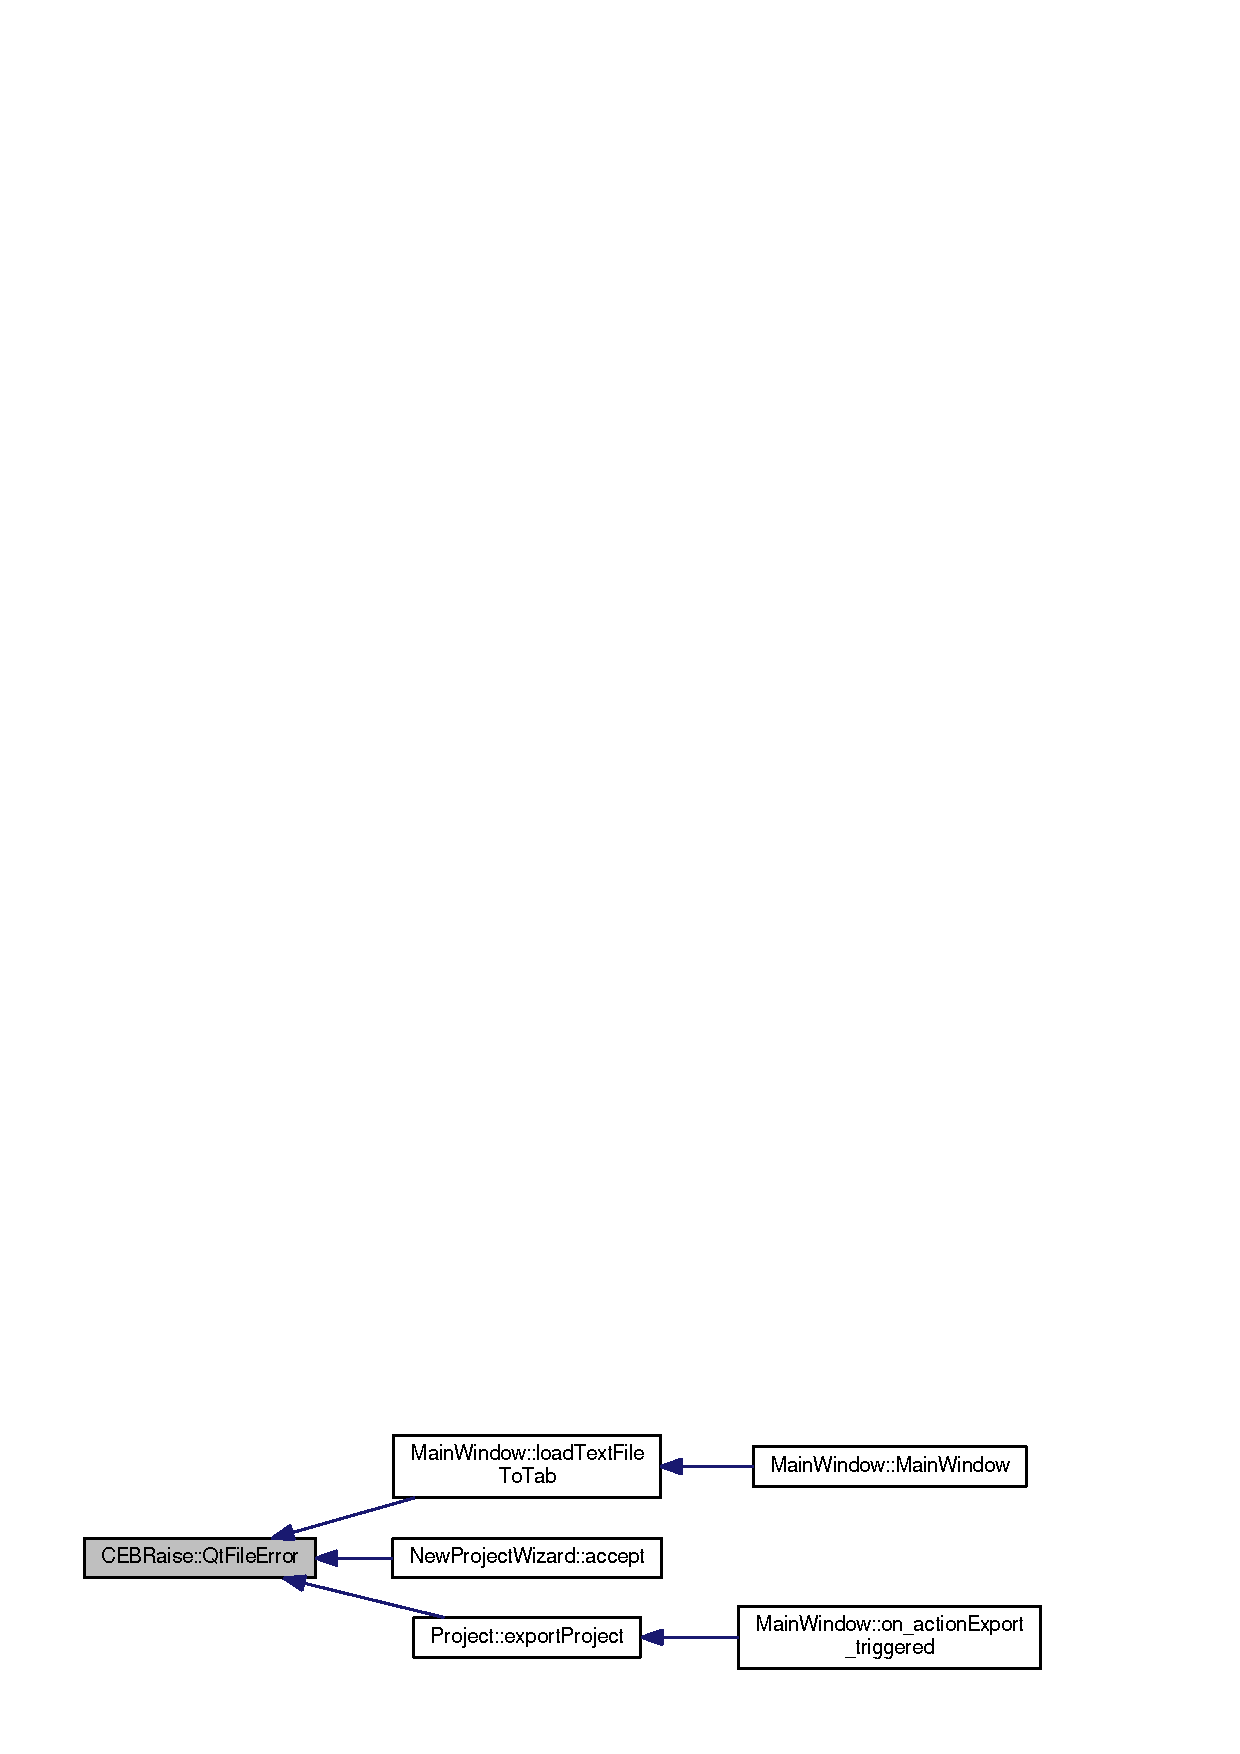
\includegraphics[width=350pt]{namespace_c_e_b_raise_a664ab19610a5a1b25b082ca8bdf51e7b_icgraph}
\end{center}
\end{figure}



\section{Ui Namespace Reference}
\label{namespace_ui}\index{Ui@{Ui}}


Used to inherit the \doxyref{Main\-Window}{p.}{class_main_window} from the generated form file ui\-\_\-\-Main\-Window.\-h.  




\subsection{Detailed Description}
Used to inherit the \doxyref{Main\-Window}{p.}{class_main_window} from the generated form file ui\-\_\-\-Main\-Window.\-h. 
\chapter{Class Documentation}
\section{C\-E\-B\-Error\-:\-:base\-Error Class Reference}
\label{class_c_e_b_error_1_1base_error}\index{C\-E\-B\-Error\-::base\-Error@{C\-E\-B\-Error\-::base\-Error}}


an unknown error which is raised when a throw is not based from a normal exception  




{\ttfamily \#include $<$Ceb\-Errors.\-h$>$}



Inheritance diagram for C\-E\-B\-Error\-:\-:base\-Error\-:\nopagebreak
\begin{figure}[H]
\begin{center}
\leavevmode
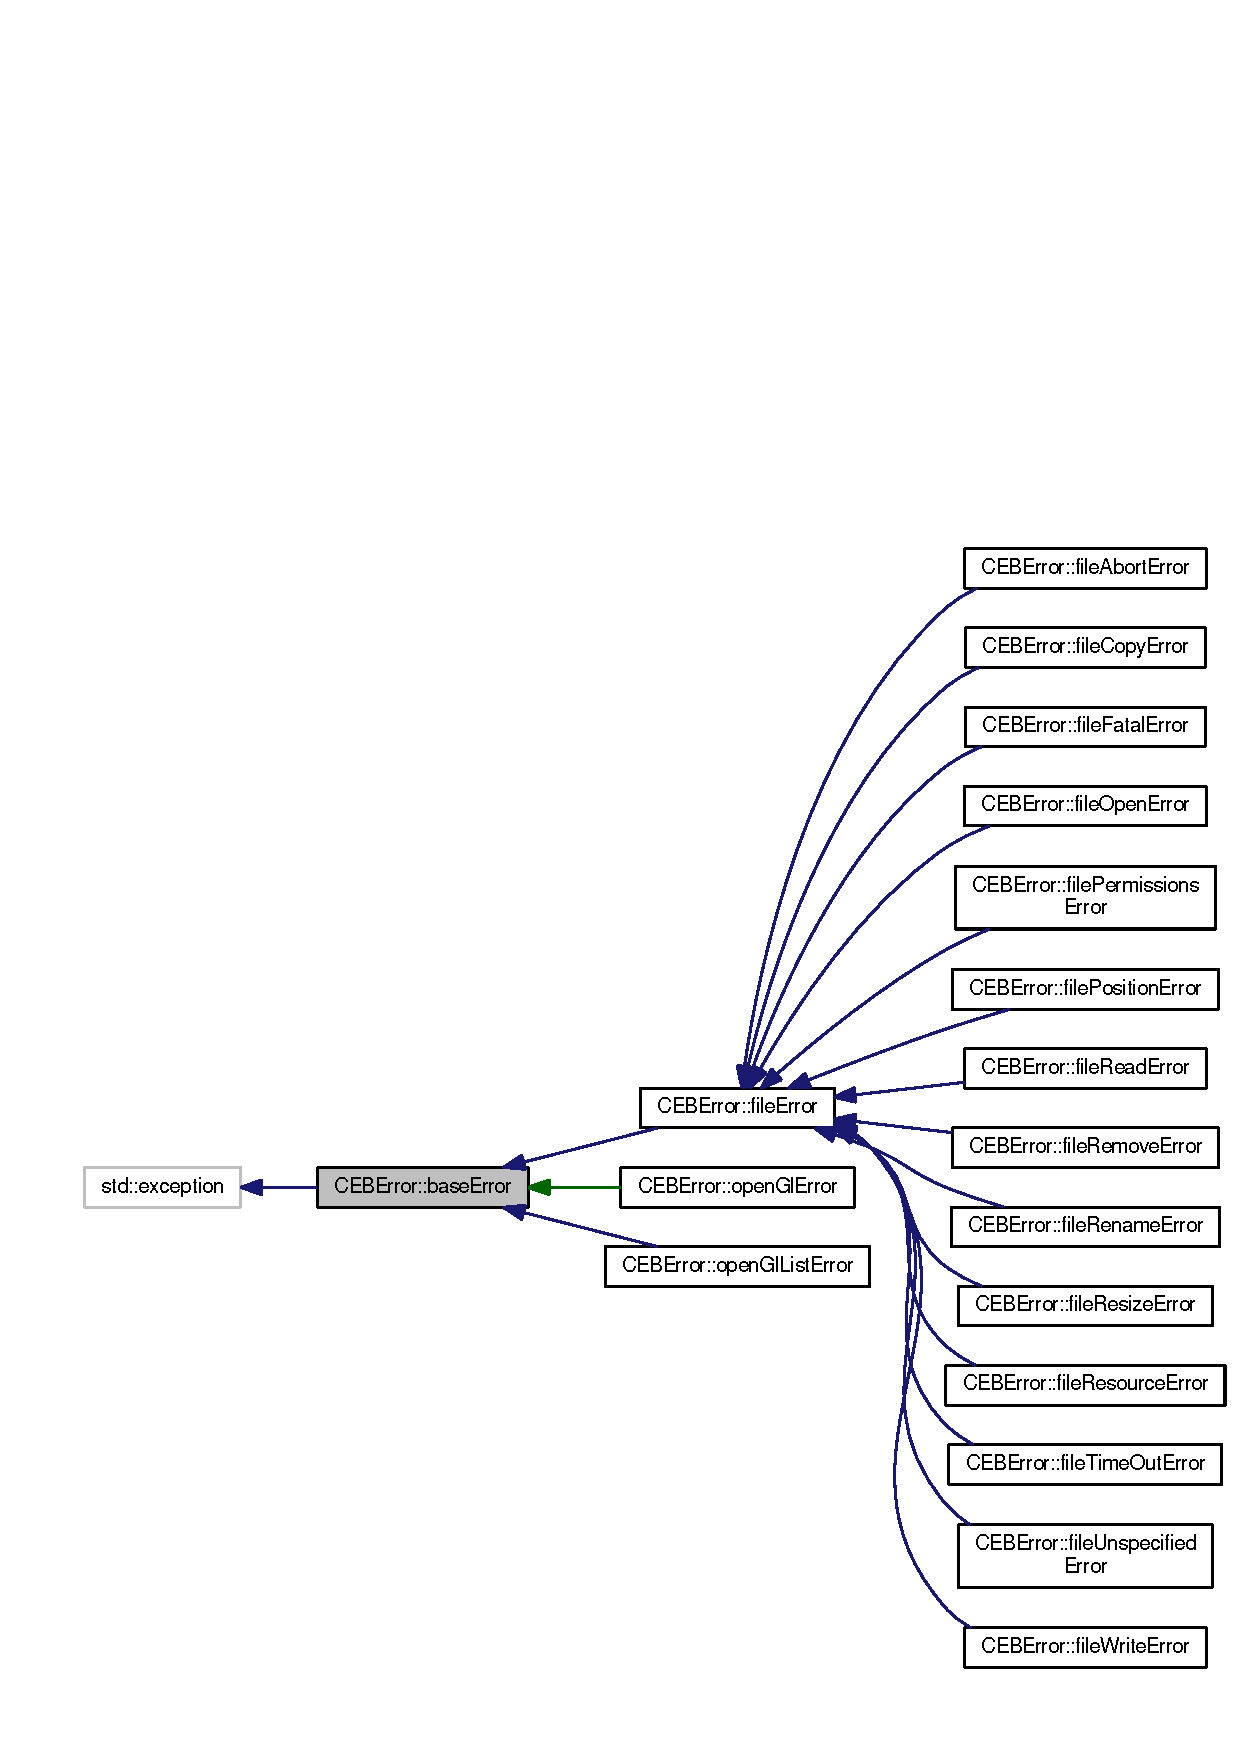
\includegraphics[width=350pt]{class_c_e_b_error_1_1base_error__inherit__graph}
\end{center}
\end{figure}


Collaboration diagram for C\-E\-B\-Error\-:\-:base\-Error\-:\nopagebreak
\begin{figure}[H]
\begin{center}
\leavevmode
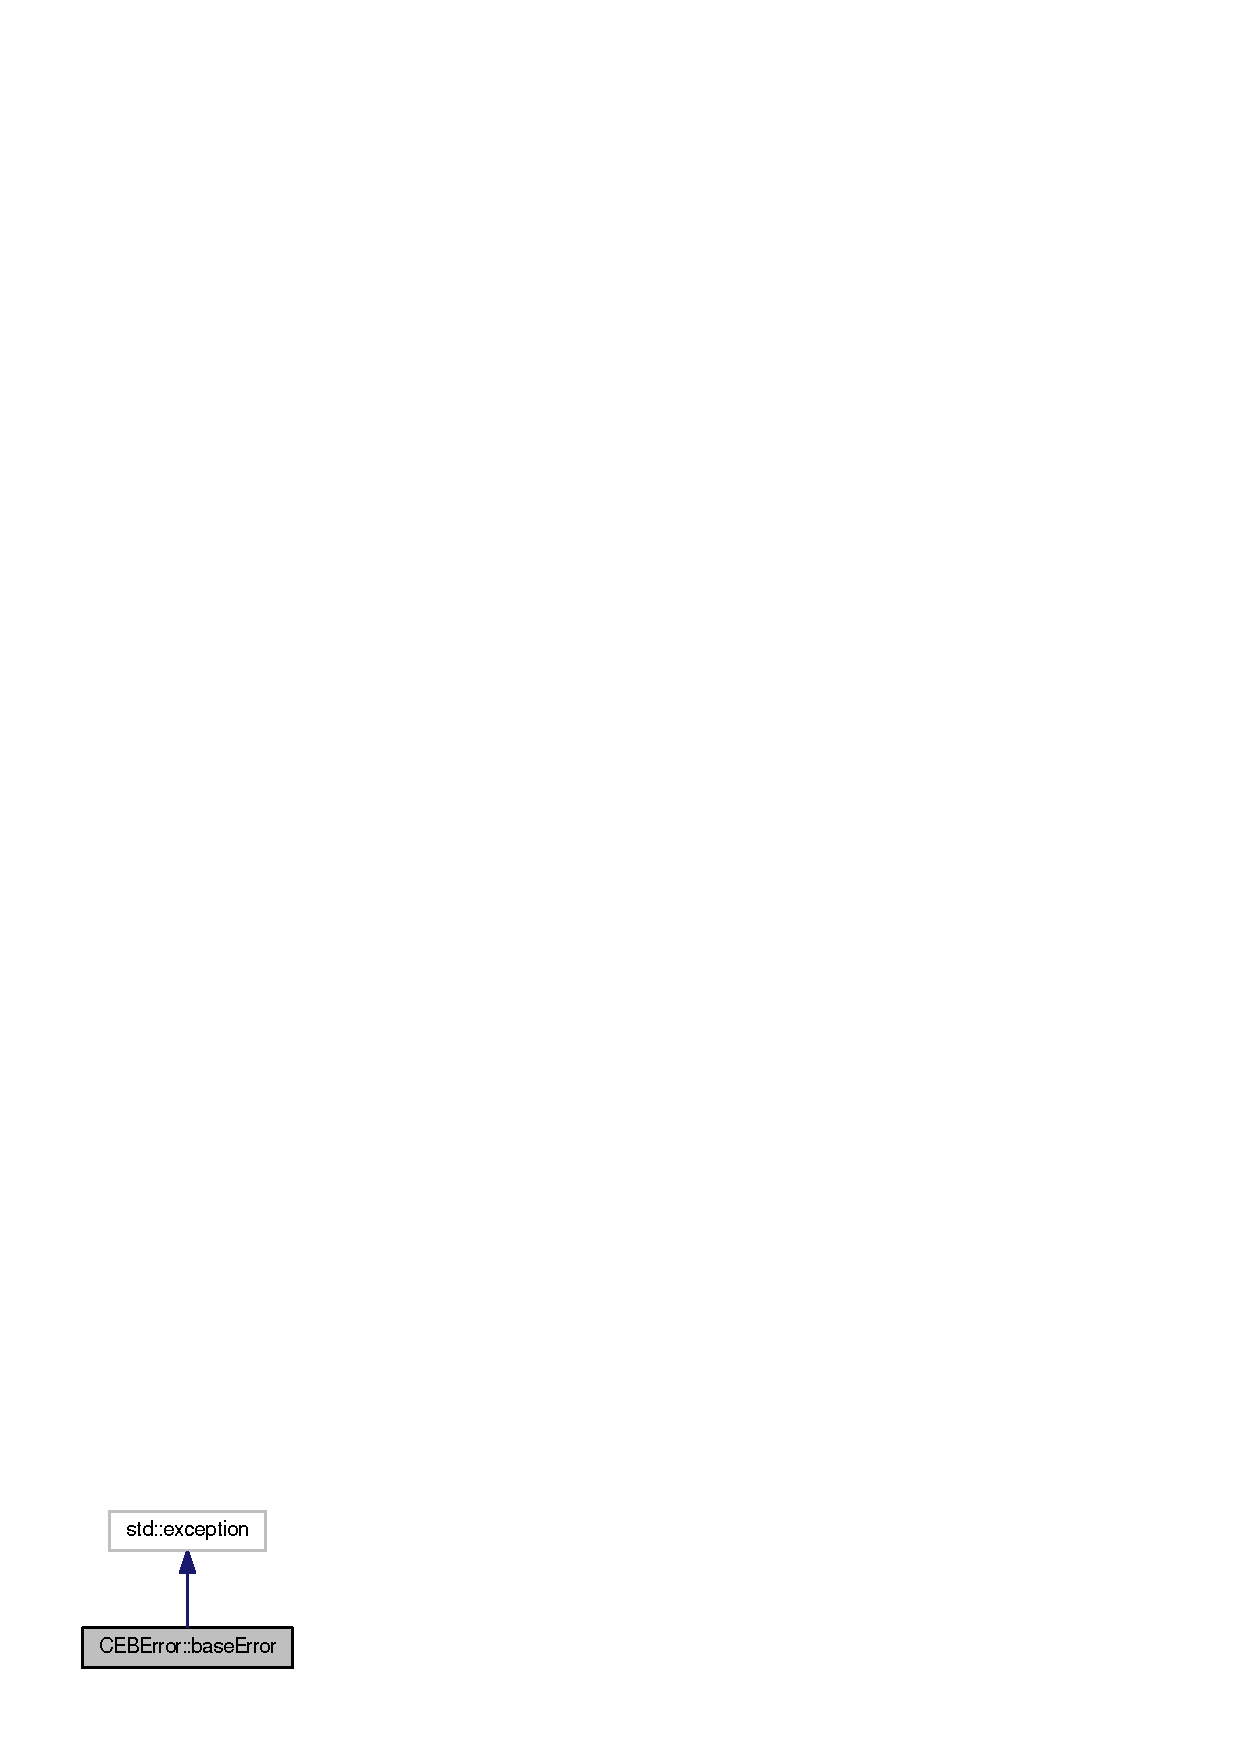
\includegraphics[width=144pt]{class_c_e_b_error_1_1base_error__coll__graph}
\end{center}
\end{figure}
\subsection*{Public Member Functions}
\begin{DoxyCompactItemize}
\item 
{\bf base\-Error} ()
\begin{DoxyCompactList}\small\item\em Constructor for file error. \end{DoxyCompactList}\item 
{\bf base\-Error} (Q\-String \-\_\-txt)
\begin{DoxyCompactList}\small\item\em Constructor for file error. \end{DoxyCompactList}\item 
virtual const char $\ast$ {\bf what} () const   throw ()
\begin{DoxyCompactList}\small\item\em returns an explanatory string \end{DoxyCompactList}\end{DoxyCompactItemize}
\subsection*{Protected Member Functions}
\begin{DoxyCompactItemize}
\item 
const char $\ast$ {\bf generate\-Msg} (std\-::string \-\_\-msg) const 
\begin{DoxyCompactList}\small\item\em generates the error message for files \end{DoxyCompactList}\end{DoxyCompactItemize}
\subsection*{Protected Attributes}
\begin{DoxyCompactItemize}
\item 
Q\-String {\bf m\-\_\-txt}
\begin{DoxyCompactList}\small\item\em the file path location where the file exists \end{DoxyCompactList}\end{DoxyCompactItemize}


\subsection{Detailed Description}
an unknown error which is raised when a throw is not based from a normal exception 

Definition at line 83 of file Ceb\-Errors.\-h.



\subsection{Constructor \& Destructor Documentation}
\index{C\-E\-B\-Error\-::base\-Error@{C\-E\-B\-Error\-::base\-Error}!base\-Error@{base\-Error}}
\index{base\-Error@{base\-Error}!CEBError::baseError@{C\-E\-B\-Error\-::base\-Error}}
\subsubsection[{base\-Error}]{\setlength{\rightskip}{0pt plus 5cm}C\-E\-B\-Error\-::base\-Error\-::base\-Error (
\begin{DoxyParamCaption}
{}
\end{DoxyParamCaption}
)\hspace{0.3cm}{\ttfamily [inline]}}\label{class_c_e_b_error_1_1base_error_aa03f3791ed755ed44d67754134c017f5}


Constructor for file error. 


\begin{DoxyParams}[1]{Parameters}
\mbox{\tt in}  & {\em \-\_\-path} & the location of the file \\
\hline
\end{DoxyParams}


Definition at line 92 of file Ceb\-Errors.\-h.


\begin{DoxyCode}
92              :
93     m_txt(\textcolor{stringliteral}{"<NoMessage>"})\{;\}
\end{DoxyCode}
\index{C\-E\-B\-Error\-::base\-Error@{C\-E\-B\-Error\-::base\-Error}!base\-Error@{base\-Error}}
\index{base\-Error@{base\-Error}!CEBError::baseError@{C\-E\-B\-Error\-::base\-Error}}
\subsubsection[{base\-Error}]{\setlength{\rightskip}{0pt plus 5cm}C\-E\-B\-Error\-::base\-Error\-::base\-Error (
\begin{DoxyParamCaption}
\item[{Q\-String}]{\-\_\-txt}
\end{DoxyParamCaption}
)\hspace{0.3cm}{\ttfamily [inline]}}\label{class_c_e_b_error_1_1base_error_a2a8739d50dbfbac74e85353effa85110}


Constructor for file error. 


\begin{DoxyParams}[1]{Parameters}
\mbox{\tt in}  & {\em \-\_\-path} & the location of the file \\
\hline
\end{DoxyParams}


Definition at line 98 of file Ceb\-Errors.\-h.


\begin{DoxyCode}
98                          :
99     m_txt(\_txt)\{;\}
\end{DoxyCode}


\subsection{Member Function Documentation}
\index{C\-E\-B\-Error\-::base\-Error@{C\-E\-B\-Error\-::base\-Error}!generate\-Msg@{generate\-Msg}}
\index{generate\-Msg@{generate\-Msg}!CEBError::baseError@{C\-E\-B\-Error\-::base\-Error}}
\subsubsection[{generate\-Msg}]{\setlength{\rightskip}{0pt plus 5cm}const char$\ast$ C\-E\-B\-Error\-::base\-Error\-::generate\-Msg (
\begin{DoxyParamCaption}
\item[{std\-::string}]{\-\_\-msg}
\end{DoxyParamCaption}
) const\hspace{0.3cm}{\ttfamily [inline]}, {\ttfamily [protected]}}\label{class_c_e_b_error_1_1base_error_adb4a4586cb1c580201cdde8c70fc32fe}


generates the error message for files 


\begin{DoxyParams}[1]{Parameters}
\mbox{\tt in}  & {\em \-\_\-msg} & the reason the error has been raised \\
\hline
\end{DoxyParams}


Definition at line 118 of file Ceb\-Errors.\-h.



References m\-\_\-txt.


\begin{DoxyCode}
119   \{
120     std::string msg = \_msg + \textcolor{stringliteral}{" '"} + m_txt.toUtf8().constData() + \textcolor{stringliteral}{"'"};
121     \textcolor{keywordflow}{return} msg.c\_str();
122   \}
\end{DoxyCode}


Here is the caller graph for this function\-:\nopagebreak
\begin{figure}[H]
\begin{center}
\leavevmode
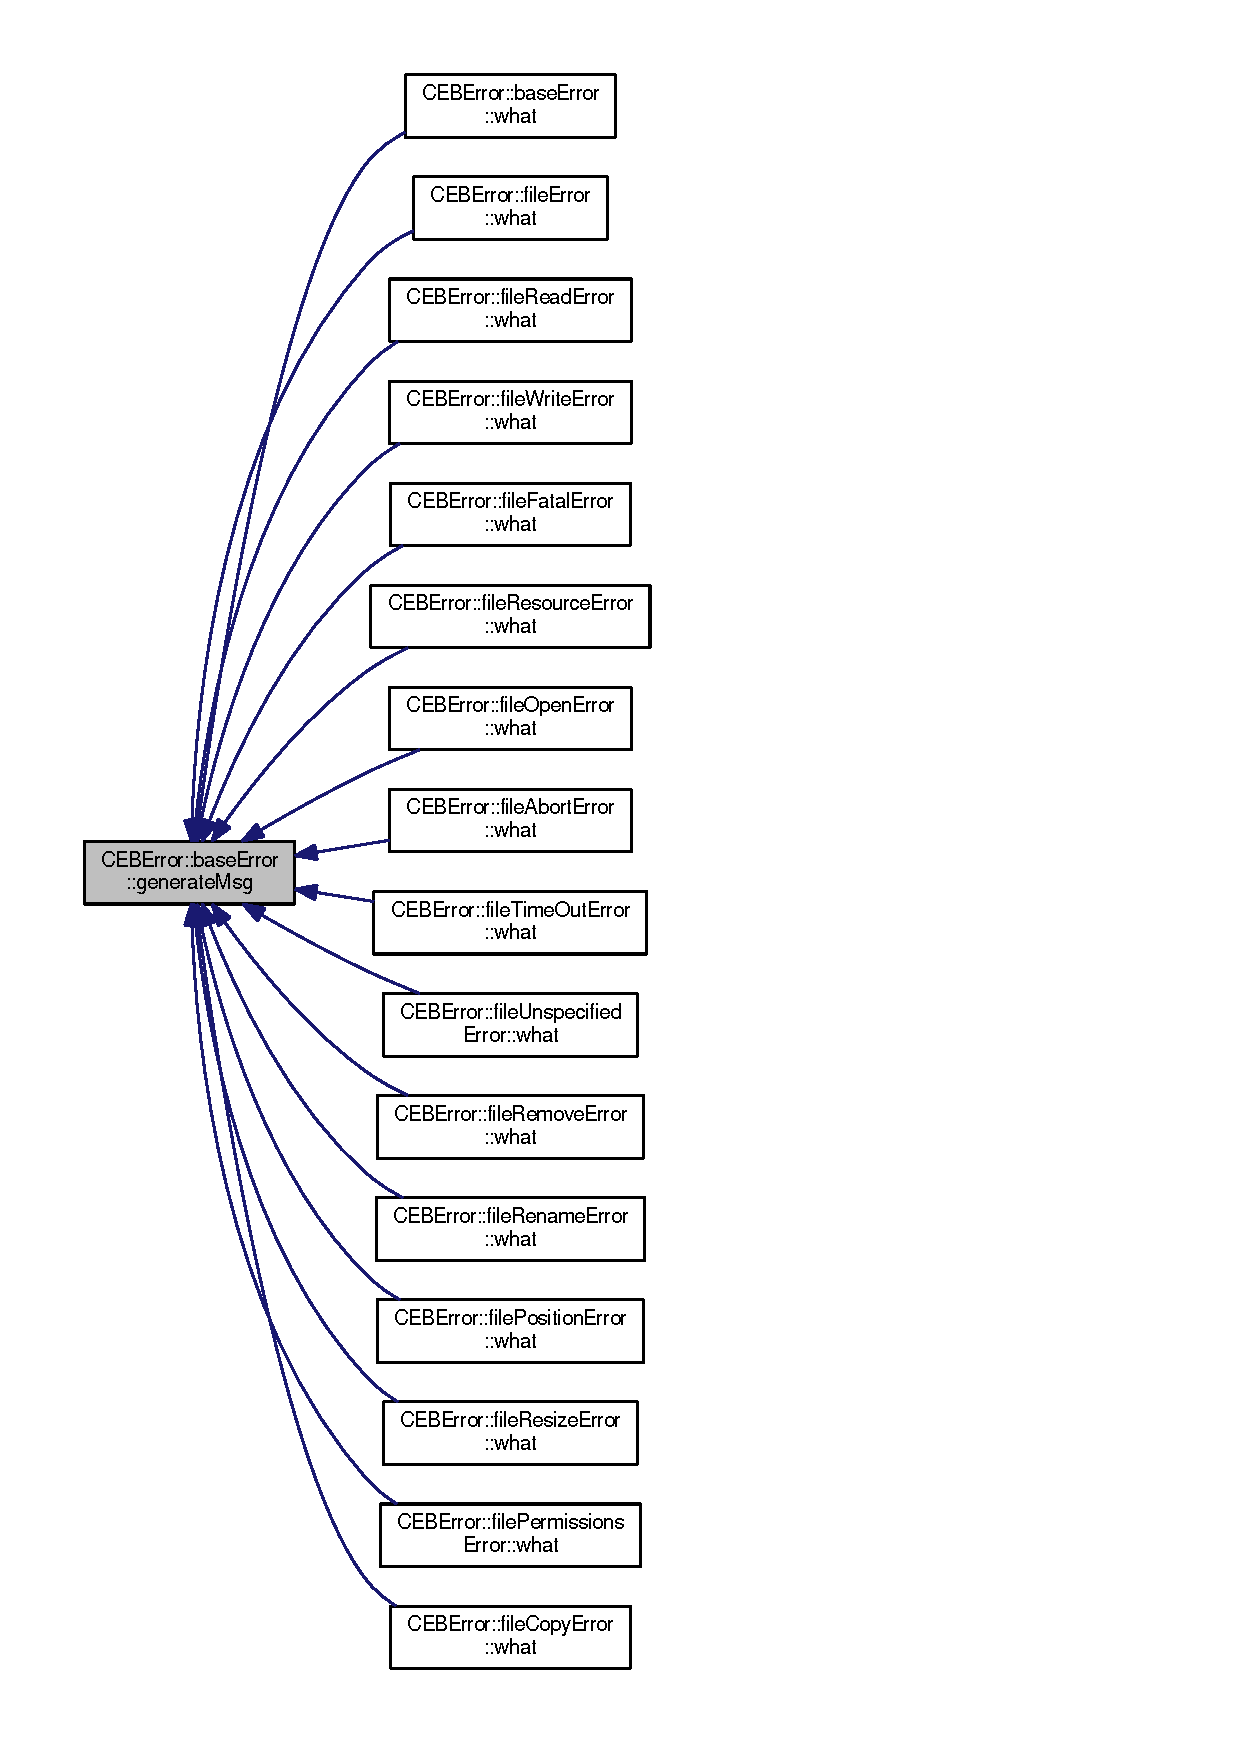
\includegraphics[height=550pt]{class_c_e_b_error_1_1base_error_adb4a4586cb1c580201cdde8c70fc32fe_icgraph}
\end{center}
\end{figure}


\index{C\-E\-B\-Error\-::base\-Error@{C\-E\-B\-Error\-::base\-Error}!what@{what}}
\index{what@{what}!CEBError::baseError@{C\-E\-B\-Error\-::base\-Error}}
\subsubsection[{what}]{\setlength{\rightskip}{0pt plus 5cm}virtual const char$\ast$ C\-E\-B\-Error\-::base\-Error\-::what (
\begin{DoxyParamCaption}
{}
\end{DoxyParamCaption}
) const throw  ) \hspace{0.3cm}{\ttfamily [inline]}, {\ttfamily [virtual]}}\label{class_c_e_b_error_1_1base_error_aaebf355e6b7b5c89d333fd258eefdaa8}


returns an explanatory string 



Reimplemented in {\bf C\-E\-B\-Error\-::open\-Gl\-List\-Error} \doxyref{}{p.}{class_c_e_b_error_1_1open_gl_list_error_acc315fa277956e59657deea4c63f96ef}, {\bf C\-E\-B\-Error\-::open\-Gl\-Error} \doxyref{}{p.}{class_c_e_b_error_1_1open_gl_error_a63d2ba5d470312311ee2fb05ac40169c}, {\bf C\-E\-B\-Error\-::file\-Copy\-Error} \doxyref{}{p.}{class_c_e_b_error_1_1file_copy_error_a0222f2bec1c517def68ab5a68bea8d22}, {\bf C\-E\-B\-Error\-::file\-Permissions\-Error} \doxyref{}{p.}{class_c_e_b_error_1_1file_permissions_error_a5d2198d1bd04e1bb0d1fd21b443247b5}, {\bf C\-E\-B\-Error\-::file\-Resize\-Error} \doxyref{}{p.}{class_c_e_b_error_1_1file_resize_error_a10cb33967f1c4c0f5c2a6092986d74ee}, {\bf C\-E\-B\-Error\-::file\-Position\-Error} \doxyref{}{p.}{class_c_e_b_error_1_1file_position_error_a16d57a675c34aa9223b41c23396120d5}, {\bf C\-E\-B\-Error\-::file\-Rename\-Error} \doxyref{}{p.}{class_c_e_b_error_1_1file_rename_error_a8e3e40fe64af2d371292f0b7870b48dc}, {\bf C\-E\-B\-Error\-::file\-Remove\-Error} \doxyref{}{p.}{class_c_e_b_error_1_1file_remove_error_ab0d8b96b77fa71a987a2b615d4c3ed6f}, {\bf C\-E\-B\-Error\-::file\-Unspecified\-Error} \doxyref{}{p.}{class_c_e_b_error_1_1file_unspecified_error_a5fd01a2dc4466c05771c747d77f8c1c8}, {\bf C\-E\-B\-Error\-::file\-Time\-Out\-Error} \doxyref{}{p.}{class_c_e_b_error_1_1file_time_out_error_a3faa61ff4b2957c8e8378a5469d1e555}, {\bf C\-E\-B\-Error\-::file\-Abort\-Error} \doxyref{}{p.}{class_c_e_b_error_1_1file_abort_error_aef6252c26fcec135375d31e180531a0b}, {\bf C\-E\-B\-Error\-::file\-Open\-Error} \doxyref{}{p.}{class_c_e_b_error_1_1file_open_error_a8b5a6e948a1579231e43900e10007e28}, {\bf C\-E\-B\-Error\-::file\-Resource\-Error} \doxyref{}{p.}{class_c_e_b_error_1_1file_resource_error_aa93a3ccb45a83aa3a2a22470e8158ab2}, {\bf C\-E\-B\-Error\-::file\-Fatal\-Error} \doxyref{}{p.}{class_c_e_b_error_1_1file_fatal_error_a2ce424f4c875db18e474dfde511ef994}, {\bf C\-E\-B\-Error\-::file\-Write\-Error} \doxyref{}{p.}{class_c_e_b_error_1_1file_write_error_a94080ee76fa9870cae6e2f8af8d0ca94}, {\bf C\-E\-B\-Error\-::file\-Read\-Error} \doxyref{}{p.}{class_c_e_b_error_1_1file_read_error_aedb4744aa826bd1aeabc060e9aab86f4}, and {\bf C\-E\-B\-Error\-::file\-Error} \doxyref{}{p.}{class_c_e_b_error_1_1file_error_ace162f612f8039db81cfd5f33a581483}.



Definition at line 103 of file Ceb\-Errors.\-h.



References generate\-Msg().


\begin{DoxyCode}
104   \{
105     \textcolor{keywordflow}{return} generateMsg(\textcolor{stringliteral}{"Base Error"});
106   \}
\end{DoxyCode}


Here is the call graph for this function\-:\nopagebreak
\begin{figure}[H]
\begin{center}
\leavevmode
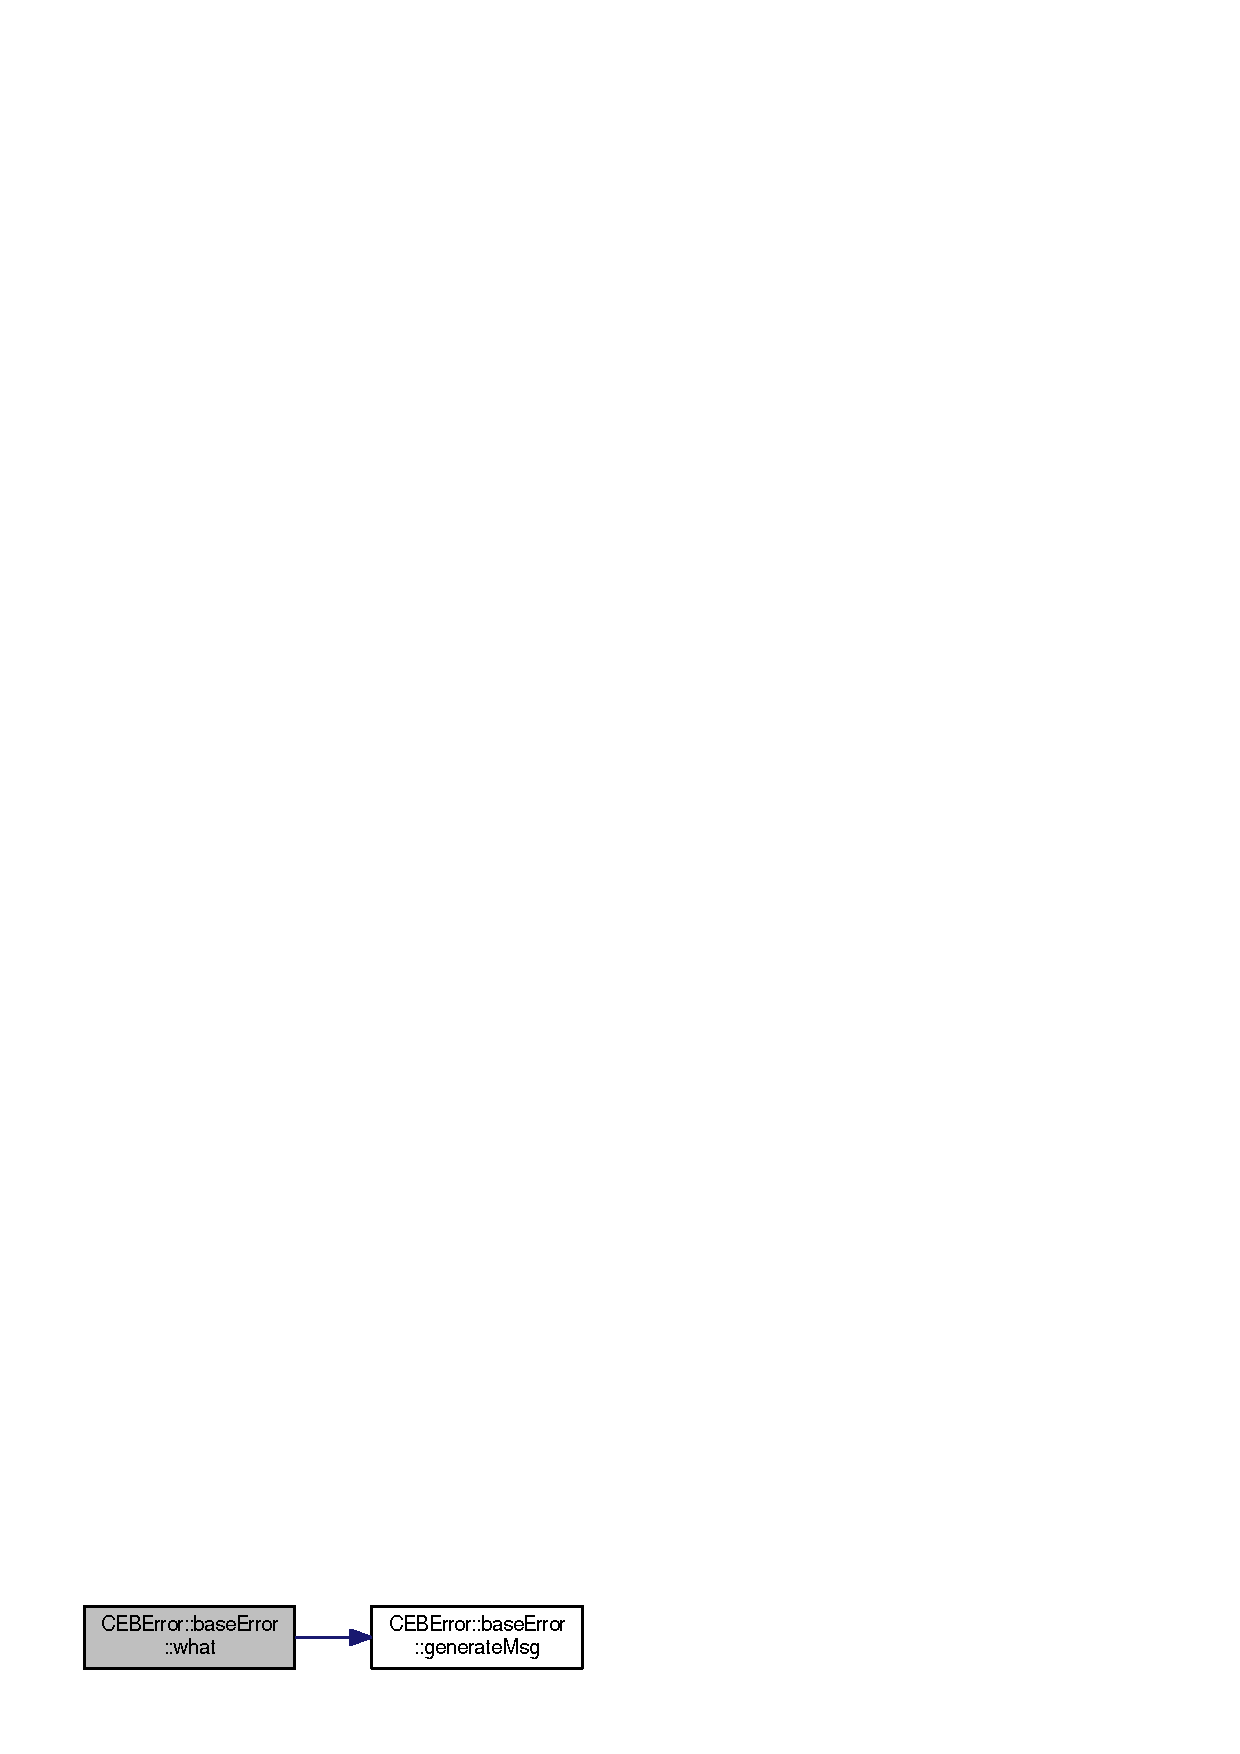
\includegraphics[width=284pt]{class_c_e_b_error_1_1base_error_aaebf355e6b7b5c89d333fd258eefdaa8_cgraph}
\end{center}
\end{figure}




\subsection{Member Data Documentation}
\index{C\-E\-B\-Error\-::base\-Error@{C\-E\-B\-Error\-::base\-Error}!m\-\_\-txt@{m\-\_\-txt}}
\index{m\-\_\-txt@{m\-\_\-txt}!CEBError::baseError@{C\-E\-B\-Error\-::base\-Error}}
\subsubsection[{m\-\_\-txt}]{\setlength{\rightskip}{0pt plus 5cm}Q\-String C\-E\-B\-Error\-::base\-Error\-::m\-\_\-txt\hspace{0.3cm}{\ttfamily [protected]}}\label{class_c_e_b_error_1_1base_error_a931f48804927a049de03f681c2c98dfc}


the file path location where the file exists 



Definition at line 113 of file Ceb\-Errors.\-h.



The documentation for this class was generated from the following file\-:\begin{DoxyCompactItemize}
\item 
{\bf Ceb\-Errors.\-h}\end{DoxyCompactItemize}

\section{Button Class Reference}
\label{class_button}\index{Button@{Button}}


Parent class of different button types to set uniform values.  




{\ttfamily \#include $<$Button.\-h$>$}



Inheritance diagram for Button\-:\nopagebreak
\begin{figure}[H]
\begin{center}
\leavevmode
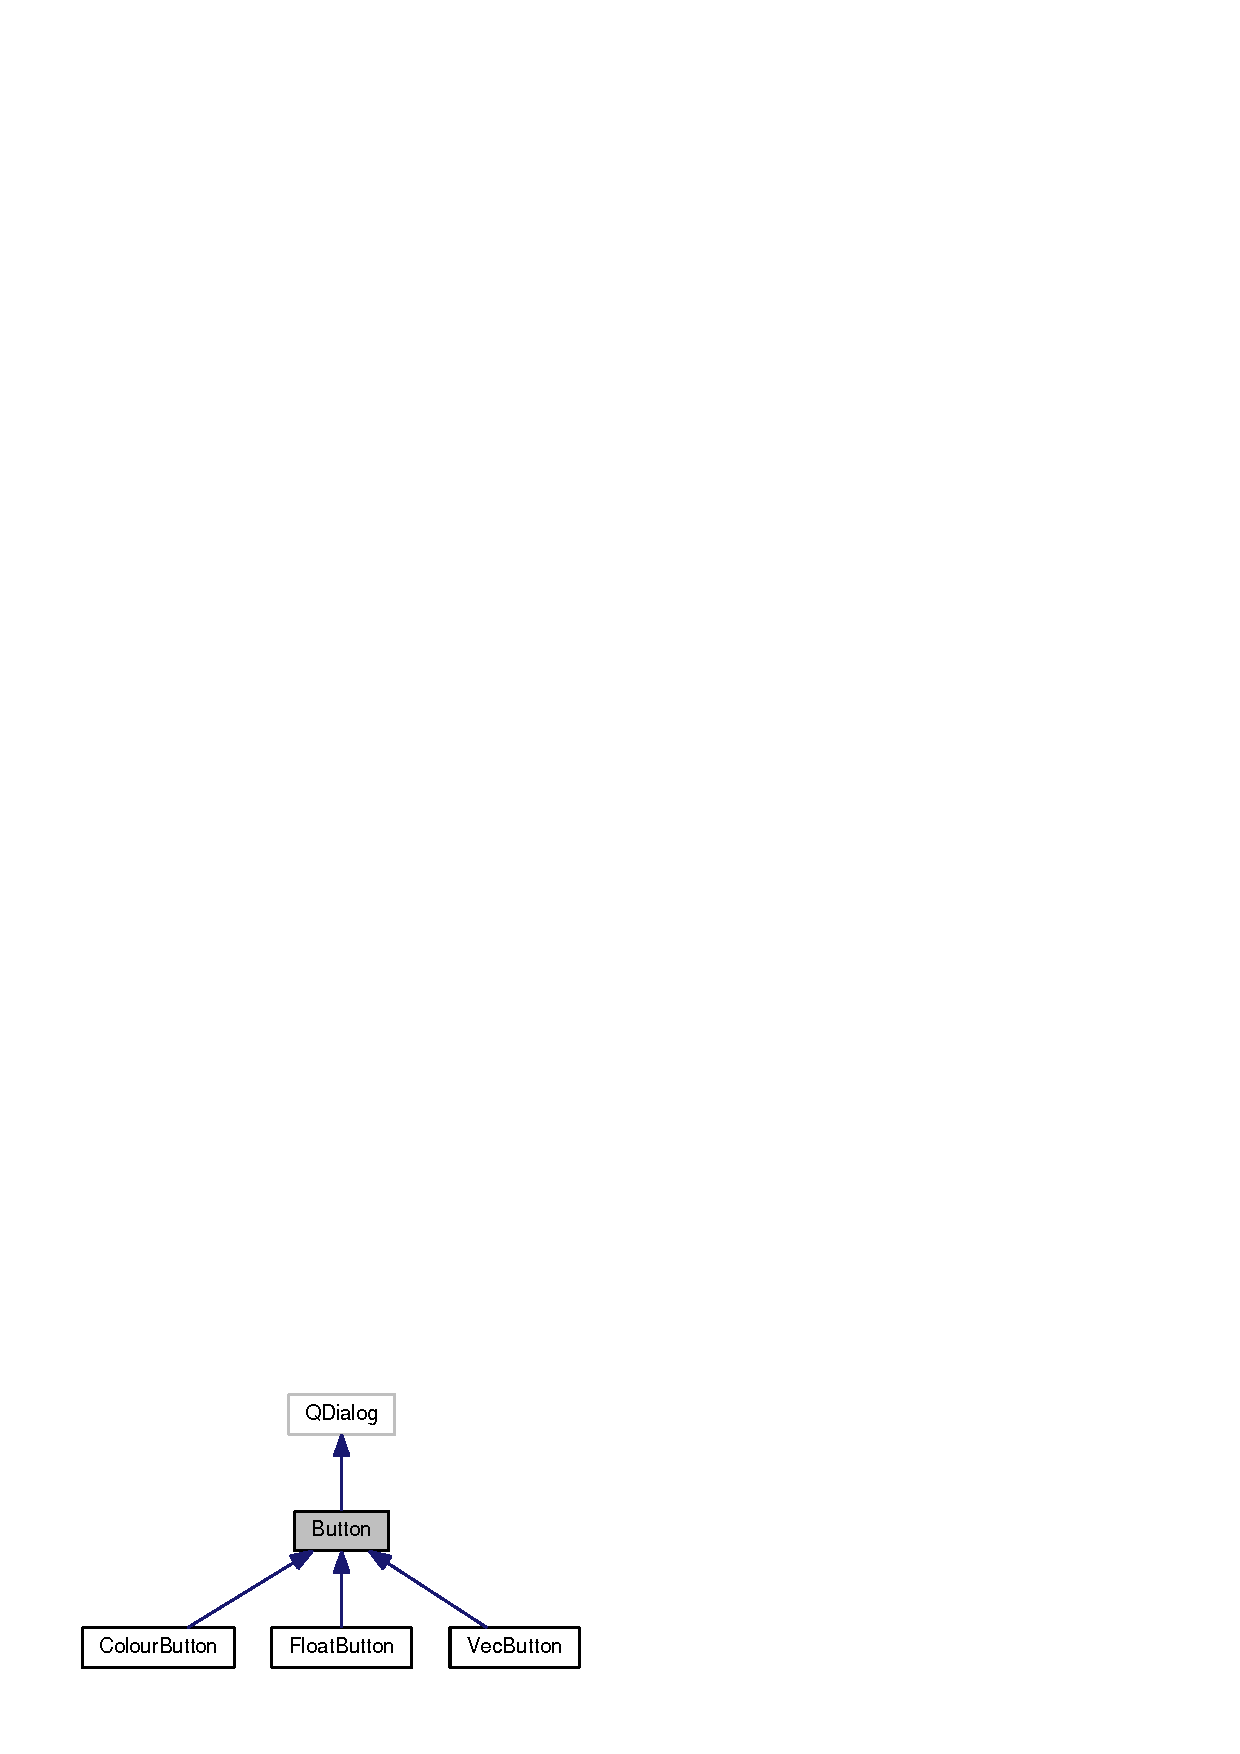
\includegraphics[width=282pt]{class_button__inherit__graph}
\end{center}
\end{figure}


Collaboration diagram for Button\-:\nopagebreak
\begin{figure}[H]
\begin{center}
\leavevmode
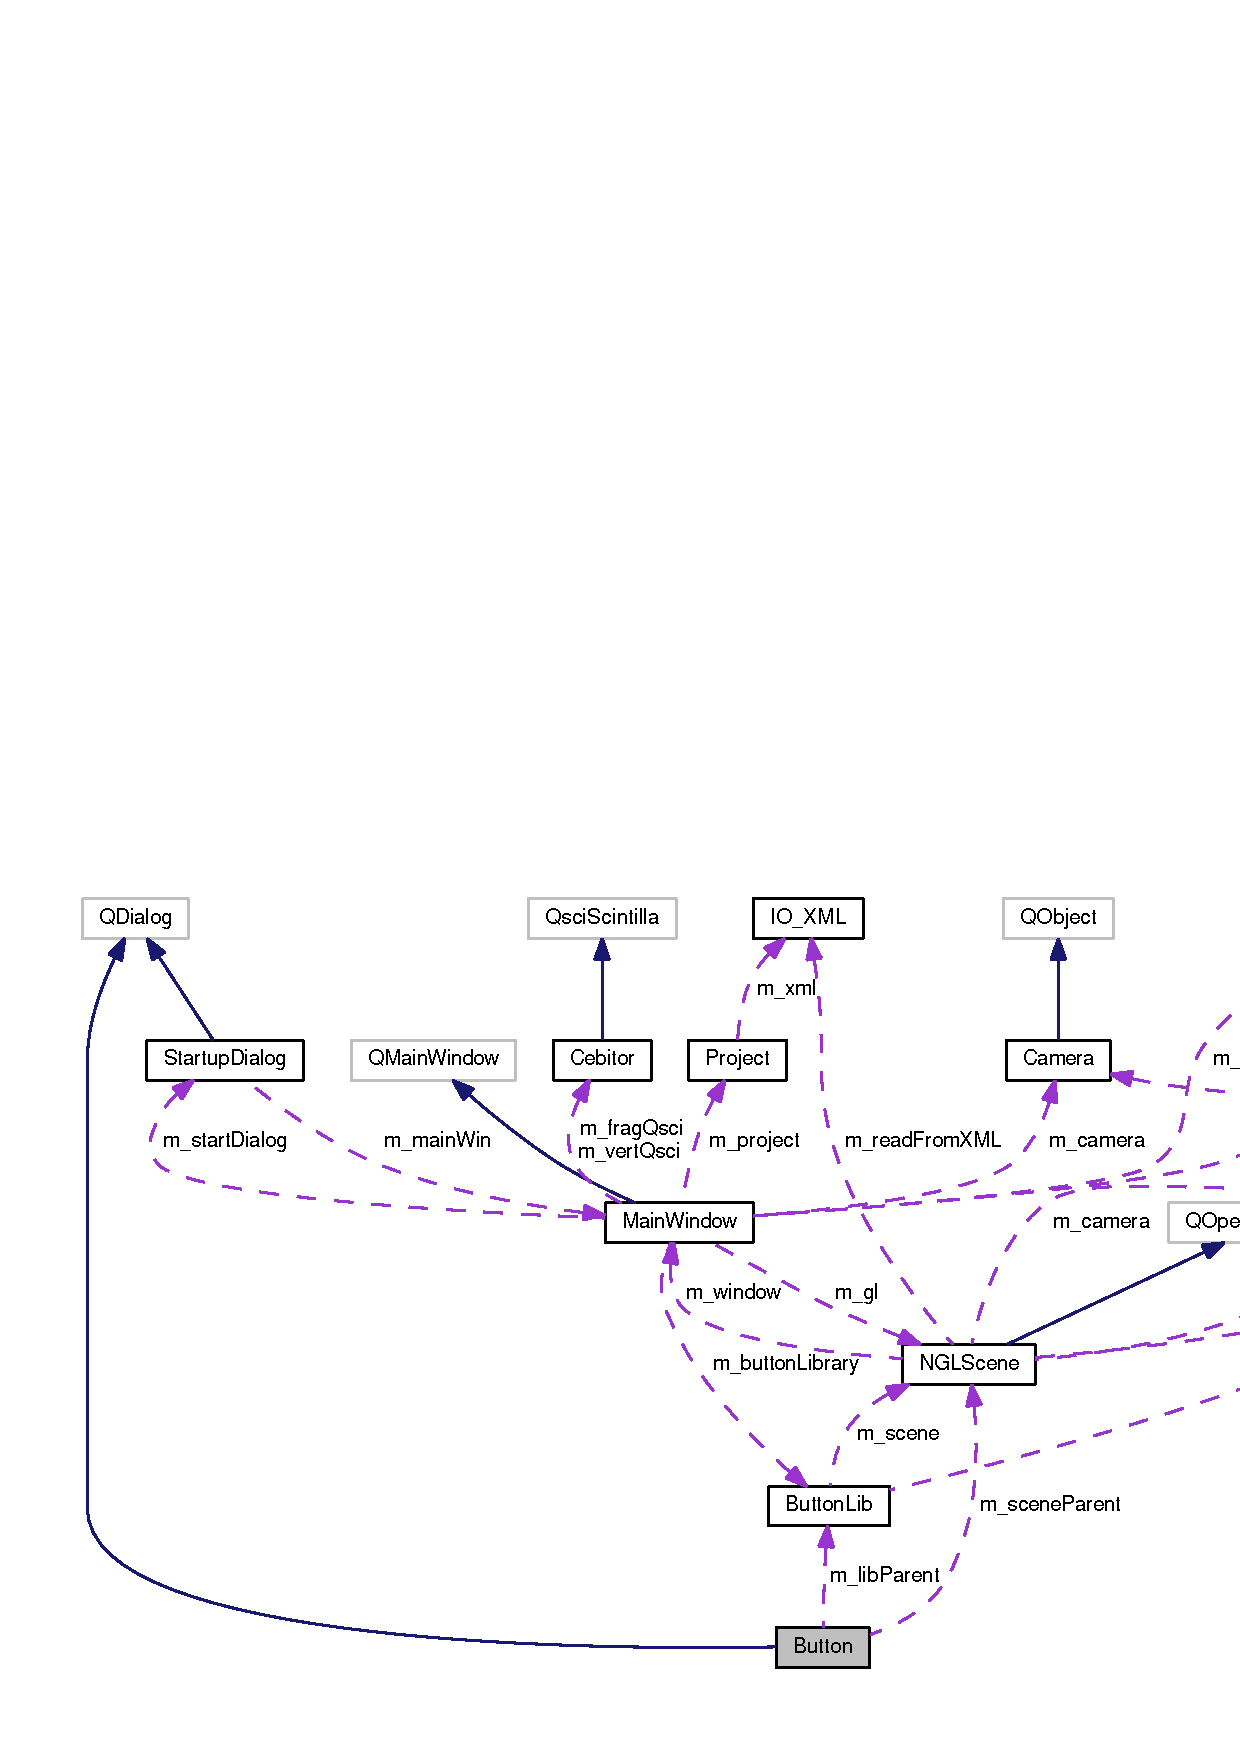
\includegraphics[width=350pt]{class_button__coll__graph}
\end{center}
\end{figure}
\subsection*{Public Member Functions}
\begin{DoxyCompactItemize}
\item 
{\bf Button} (Q\-Widget $\ast$parent=0)
\begin{DoxyCompactList}\small\item\em default constructor to create the button \end{DoxyCompactList}\item 
{\bf Button} (Q\-String \-\_\-button\-Name, G\-Lenum \-\_\-button\-Type, Q\-Layout $\ast$\-\_\-layout, G\-Luint \-\_\-id, {\bf Button\-Lib} $\ast$\-\_\-lib\-Parent, {\bf N\-G\-L\-Scene} $\ast$\-\_\-scene\-Parent, Q\-Widget $\ast$parent=0)
\begin{DoxyCompactList}\small\item\em constructor to create the button, custom variables can also be assigned \end{DoxyCompactList}\item 
Q\-String {\bf get\-Name} ()
\begin{DoxyCompactList}\small\item\em returns the current button name \end{DoxyCompactList}\item 
G\-Lenum {\bf get\-Type\-Enum} ()
\begin{DoxyCompactList}\small\item\em returns the current button type \end{DoxyCompactList}\item 
void {\bf set\-I\-D} (unsigned int \-\_\-id)
\begin{DoxyCompactList}\small\item\em sets the current I\-D for the button, from its' shader location \end{DoxyCompactList}\item 
G\-Luint {\bf get\-I\-D} ()
\begin{DoxyCompactList}\small\item\em returns the button I\-D, this will change based on shader location \end{DoxyCompactList}\item 
virtual void {\bf set\-Colour} (ngl\-::\-Vec4 \-\_\-col)
\begin{DoxyCompactList}\small\item\em sets the colour to be used by colour buttons \end{DoxyCompactList}\item 
virtual void {\bf set\-Colour} (Q\-Color \-\_\-col)
\begin{DoxyCompactList}\small\item\em overloaded function to set the colour \end{DoxyCompactList}\item 
virtual ngl\-::\-Vec4 {\bf get\-Colour} ()
\begin{DoxyCompactList}\small\item\em returns the colour, stored by the button \end{DoxyCompactList}\item 
virtual Q\-Color {\bf get\-Colour\-Q} ()
\begin{DoxyCompactList}\small\item\em returns the Q\-Colour, stored by the button \end{DoxyCompactList}\item 
virtual void {\bf set\-Value} (float \-\_\-val)
\begin{DoxyCompactList}\small\item\em sets the value to be for float attributes \end{DoxyCompactList}\item 
virtual float {\bf get\-Value} ()
\begin{DoxyCompactList}\small\item\em returns the value, stored by the button \end{DoxyCompactList}\item 
virtual void {\bf print\-Values} ()
\begin{DoxyCompactList}\small\item\em prints the button attribute values \end{DoxyCompactList}\item 
virtual ngl\-::\-Vec4 {\bf get\-Vec} ()
\begin{DoxyCompactList}\small\item\em returns the Vec4 held by the vector button class \end{DoxyCompactList}\item 
virtual void {\bf set\-Vec} (ngl\-::\-Vec4 \-\_\-value)
\begin{DoxyCompactList}\small\item\em sets the vector value for Vec3s or positions \end{DoxyCompactList}\end{DoxyCompactItemize}
\subsection*{Public Attributes}
\begin{DoxyCompactItemize}
\item 
{\bf Button\-Lib} $\ast$ {\bf m\-\_\-lib\-Parent}
\begin{DoxyCompactList}\small\item\em pointer to the button library parent \end{DoxyCompactList}\item 
{\bf N\-G\-L\-Scene} $\ast$ {\bf m\-\_\-scene\-Parent}
\begin{DoxyCompactList}\small\item\em pointer to the scene so that update can be called \end{DoxyCompactList}\item 
Q\-Widget $\ast$ {\bf m\-\_\-parent}
\begin{DoxyCompactList}\small\item\em pointer to the parent window to know where to attach to \end{DoxyCompactList}\item 
Q\-Push\-Button $\ast$ {\bf m\-\_\-button}
\begin{DoxyCompactList}\small\item\em button object to be pressed by user to open relevant widget \end{DoxyCompactList}\end{DoxyCompactItemize}
\subsection*{Private Slots}
\begin{DoxyCompactItemize}
\item 
virtual void {\bf open\-Box} ()
\begin{DoxyCompactList}\small\item\em a slot to open a widget upon button press event \end{DoxyCompactList}\end{DoxyCompactItemize}
\subsection*{Private Member Functions}
\begin{DoxyCompactItemize}
\item 
void {\bf create\-Button\-Box} (Q\-String \-\_\-button\-Name=\char`\"{}Select \&Colour\char`\"{})
\begin{DoxyCompactList}\small\item\em function to create the button box for the pop up \end{DoxyCompactList}\end{DoxyCompactItemize}
\subsection*{Private Attributes}
\begin{DoxyCompactItemize}
\item 
Q\-String {\bf m\-\_\-button\-Name}
\begin{DoxyCompactList}\small\item\em string to hold button's name \end{DoxyCompactList}\item 
G\-Lenum {\bf m\-\_\-button\-Type}
\begin{DoxyCompactList}\small\item\em enum for the button type, used for defining type \end{DoxyCompactList}\item 
unsigned int {\bf m\-\_\-id}
\begin{DoxyCompactList}\small\item\em id to access specific buttons and shader locations \end{DoxyCompactList}\item 
Q\-Dialog\-Button\-Box $\ast$ {\bf m\-\_\-button\-Box}
\begin{DoxyCompactList}\small\item\em button box used to activate the opening of the widget \end{DoxyCompactList}\item 
Q\-Grid\-Layout $\ast$ {\bf m\-\_\-grid\-Layout}
\begin{DoxyCompactList}\small\item\em layout for the button box to be stored within \end{DoxyCompactList}\end{DoxyCompactItemize}


\subsection{Detailed Description}
Parent class of different button types to set uniform values. 

Definition at line 47 of file Button.\-h.



\subsection{Constructor \& Destructor Documentation}
\index{Button@{Button}!Button@{Button}}
\index{Button@{Button}!Button@{Button}}
\subsubsection[{Button}]{\setlength{\rightskip}{0pt plus 5cm}Button\-::\-Button (
\begin{DoxyParamCaption}
\item[{Q\-Widget $\ast$}]{parent = {\ttfamily 0}}
\end{DoxyParamCaption}
)}\label{class_button_a87565544cd9fbee675f6b6d61a319efd}


default constructor to create the button 


\begin{DoxyParams}[1]{Parameters}
\mbox{\tt in}  & {\em the} & parent window is defaulted to nothing \\
\hline
\end{DoxyParams}


Definition at line 13 of file Button.\-cpp.



References create\-Button\-Box().


\begin{DoxyCode}
13                               : QDialog(parent)
14 \{
15   createButtonBox();
16 \}
\end{DoxyCode}


Here is the call graph for this function\-:\nopagebreak
\begin{figure}[H]
\begin{center}
\leavevmode
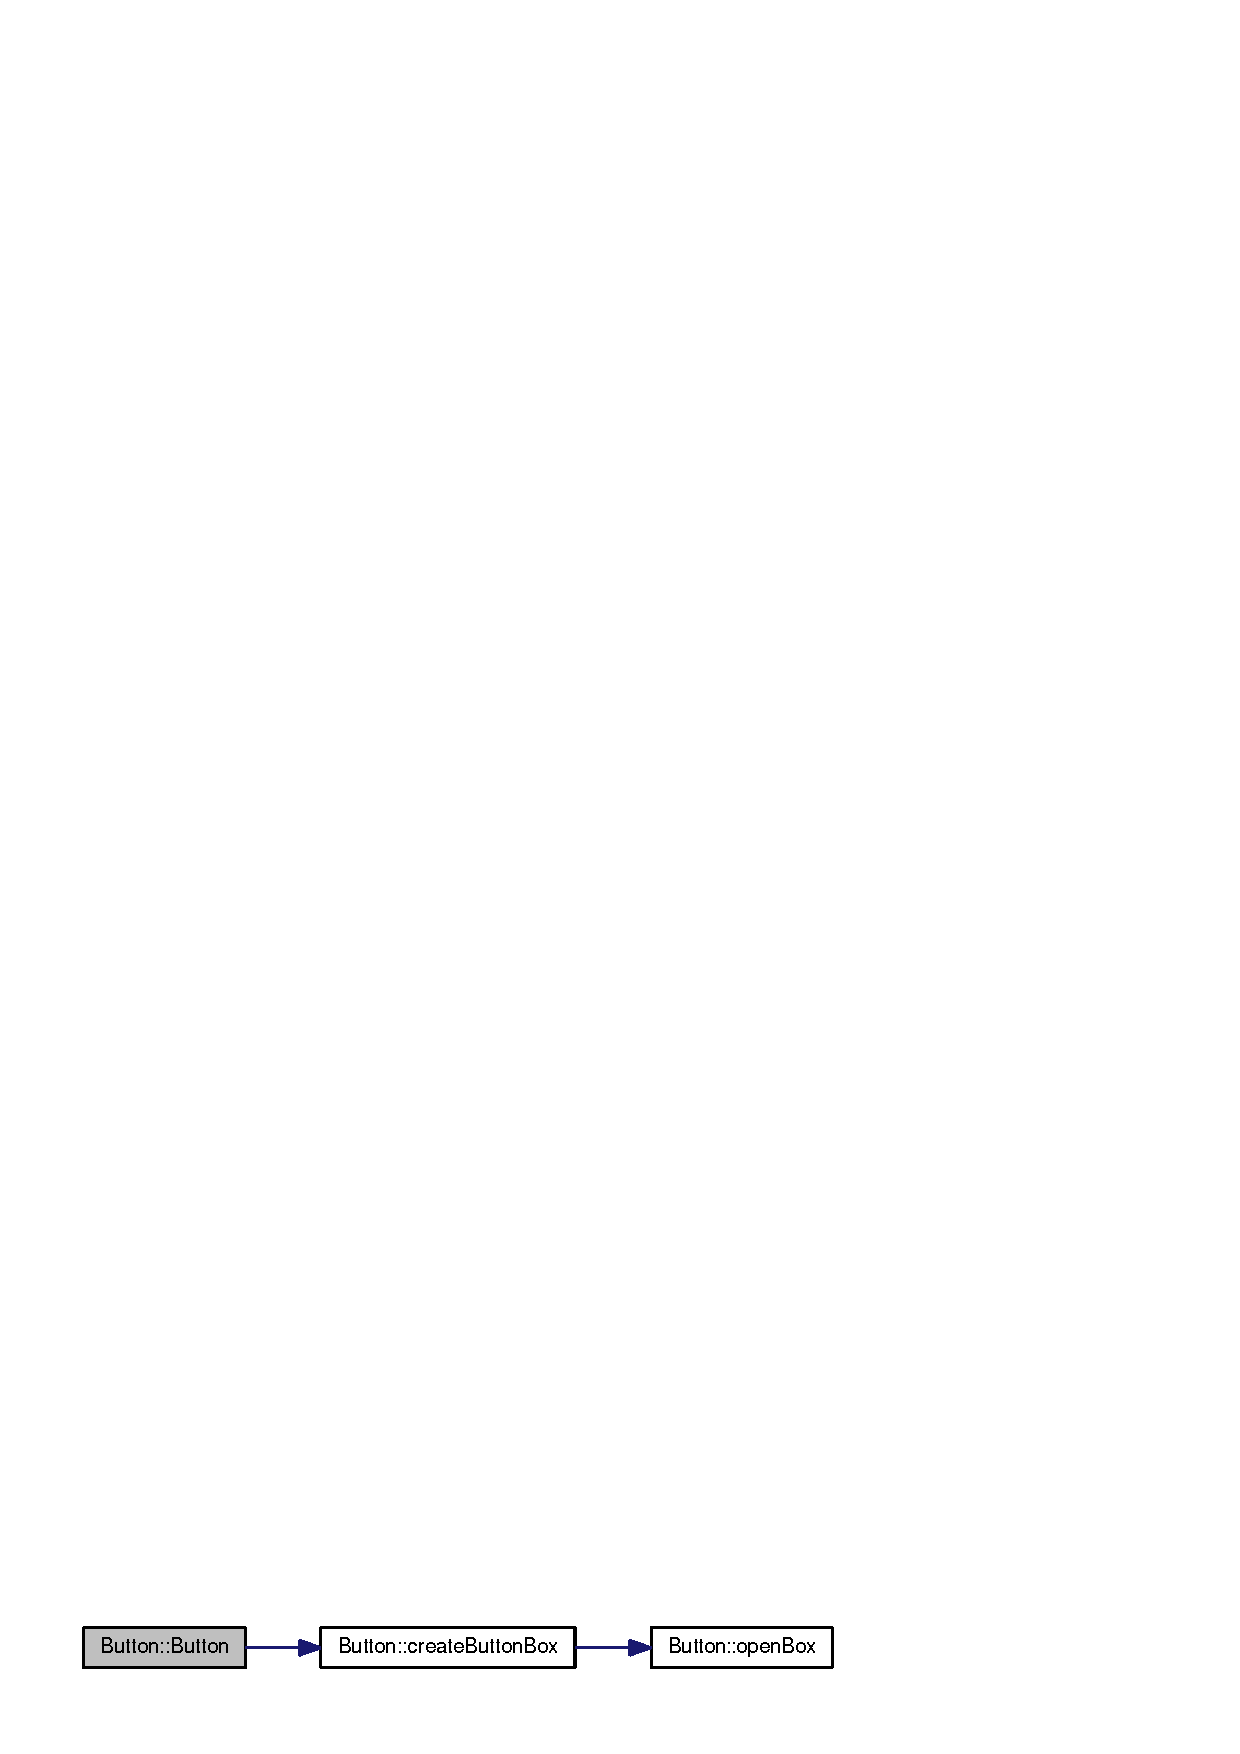
\includegraphics[width=350pt]{class_button_a87565544cd9fbee675f6b6d61a319efd_cgraph}
\end{center}
\end{figure}


\index{Button@{Button}!Button@{Button}}
\index{Button@{Button}!Button@{Button}}
\subsubsection[{Button}]{\setlength{\rightskip}{0pt plus 5cm}Button\-::\-Button (
\begin{DoxyParamCaption}
\item[{Q\-String}]{\-\_\-button\-Name, }
\item[{G\-Lenum}]{\-\_\-button\-Type, }
\item[{Q\-Layout $\ast$}]{\-\_\-layout, }
\item[{G\-Luint}]{\-\_\-id, }
\item[{{\bf Button\-Lib} $\ast$}]{\-\_\-lib\-Parent, }
\item[{{\bf N\-G\-L\-Scene} $\ast$}]{\-\_\-scene\-Parent, }
\item[{Q\-Widget $\ast$}]{parent = {\ttfamily 0}}
\end{DoxyParamCaption}
)}\label{class_button_a6a5d637d5786edca41de726b76e034a2}


constructor to create the button, custom variables can also be assigned 


\begin{DoxyParams}[1]{Parameters}
\mbox{\tt in}  & {\em name} & of the button to be used \\
\hline
\mbox{\tt in}  & {\em the} & layout environment for the button to be attached to \\
\hline
\mbox{\tt in}  & {\em the} & id used to access the button information \\
\hline
\mbox{\tt in}  & {\em the} & parent window is defaulted to nothing \\
\hline
\end{DoxyParams}


Definition at line 18 of file Button.\-cpp.



References create\-Button\-Box(), m\-\_\-button, m\-\_\-button\-Name, m\-\_\-button\-Type, m\-\_\-id, m\-\_\-lib\-Parent, m\-\_\-parent, and m\-\_\-scene\-Parent.


\begin{DoxyCode}
18                                                                                                            
                                               : QDialog(parent)
19 \{
20   m_buttonName = \_buttonName;
21   m_buttonType = \_buttonType;
22   m_id=\_id;
23   createButtonBox(\_buttonName);
24   m_libParent=\_libParent;
25   m_sceneParent=\_sceneParent;
26   m_parent=parent;
27   \_layout->addWidget(m_button);
28 \}
\end{DoxyCode}


Here is the call graph for this function\-:\nopagebreak
\begin{figure}[H]
\begin{center}
\leavevmode
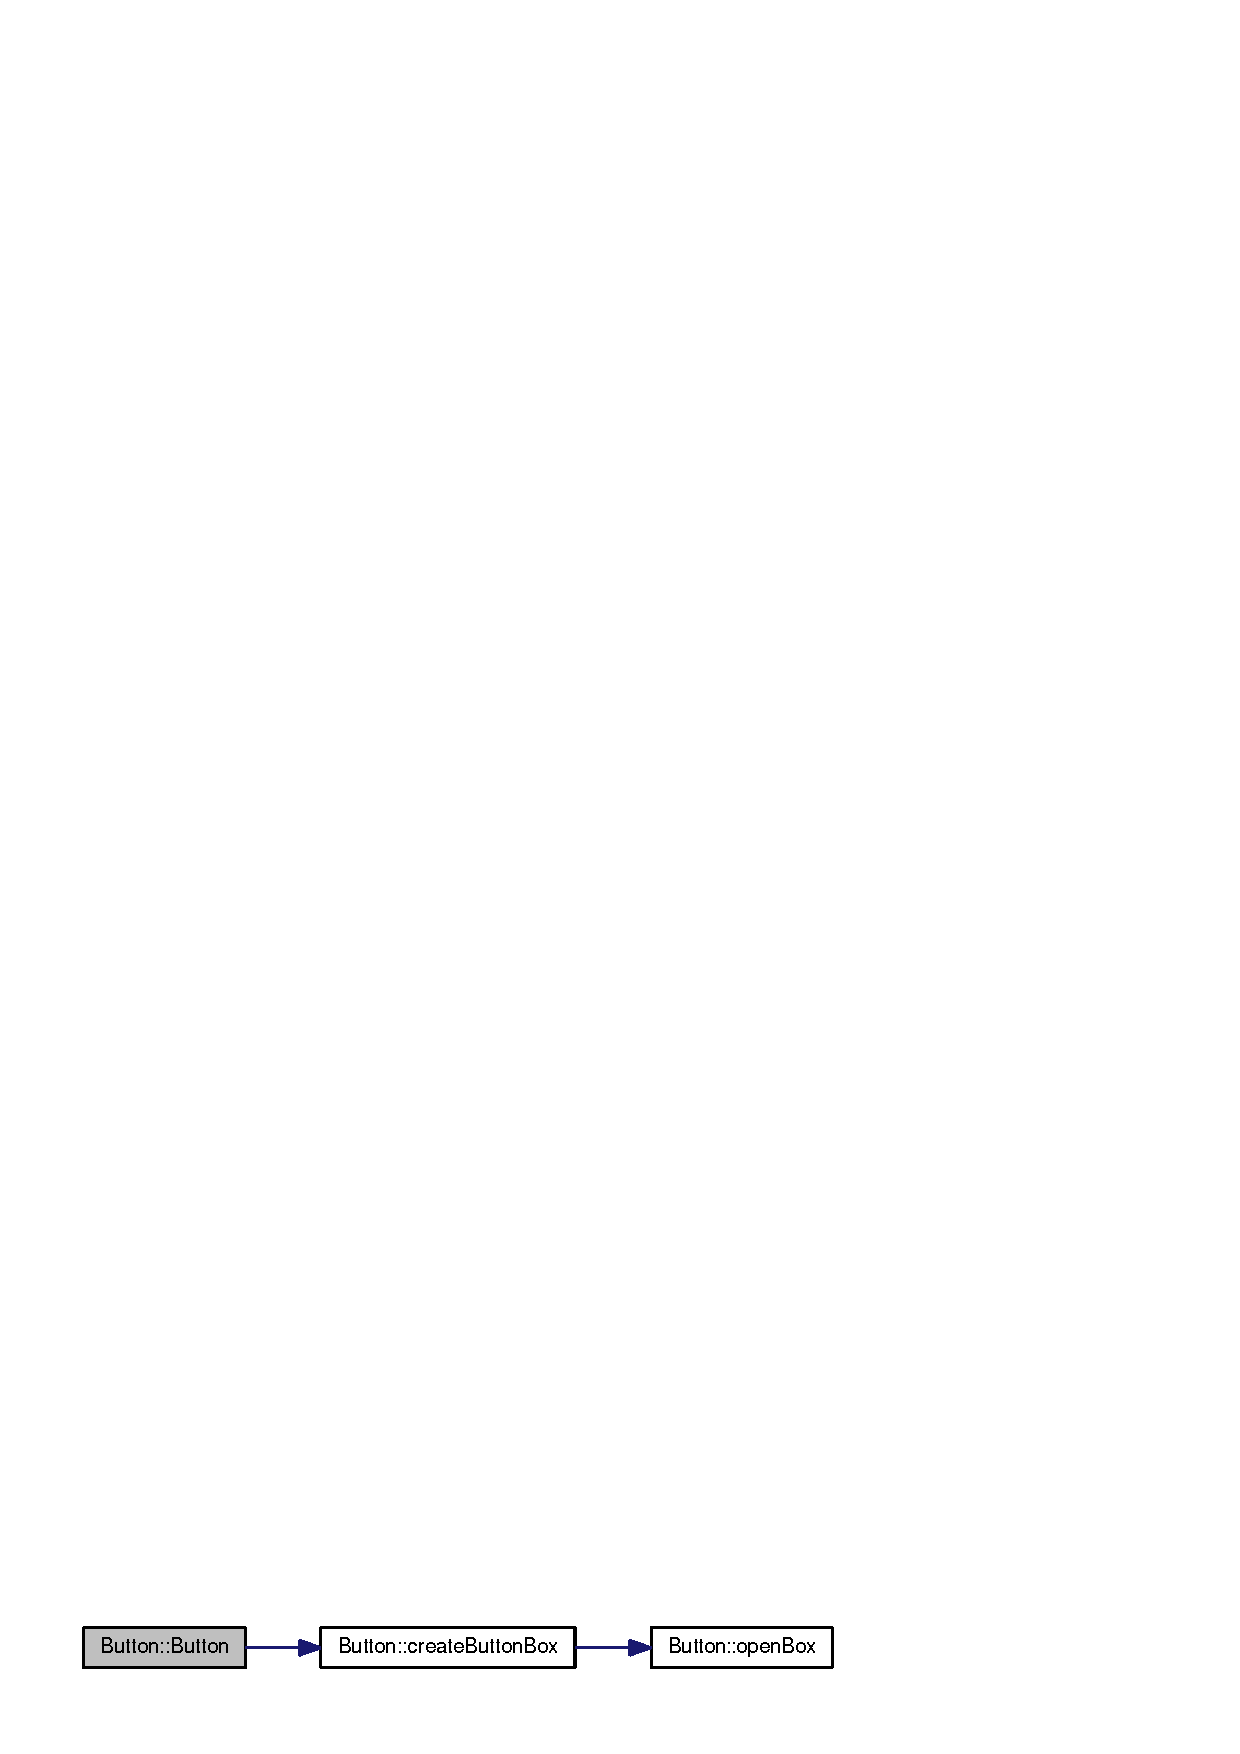
\includegraphics[width=350pt]{class_button_a6a5d637d5786edca41de726b76e034a2_cgraph}
\end{center}
\end{figure}




\subsection{Member Function Documentation}
\index{Button@{Button}!create\-Button\-Box@{create\-Button\-Box}}
\index{create\-Button\-Box@{create\-Button\-Box}!Button@{Button}}
\subsubsection[{create\-Button\-Box}]{\setlength{\rightskip}{0pt plus 5cm}void Button\-::create\-Button\-Box (
\begin{DoxyParamCaption}
\item[{Q\-String}]{\-\_\-button\-Name = {\ttfamily \char`\"{}Select~\&Colour\char`\"{}}}
\end{DoxyParamCaption}
)\hspace{0.3cm}{\ttfamily [private]}}\label{class_button_a10293cc4dcea650ad6b858430bb2a488}


function to create the button box for the pop up 


\begin{DoxyParams}[1]{Parameters}
\mbox{\tt in}  & {\em button} & name \\
\hline
\end{DoxyParams}


Definition at line 30 of file Button.\-cpp.



References m\-\_\-button, and open\-Box().


\begin{DoxyCode}
31 \{
32   m_button = \textcolor{keyword}{new} QPushButton();
33   m_button->setText(\_buttonName);
34   connect(m_button, SIGNAL(clicked()), \textcolor{keyword}{this}, SLOT(openBox()));
35 \}
\end{DoxyCode}


Here is the call graph for this function\-:\nopagebreak
\begin{figure}[H]
\begin{center}
\leavevmode
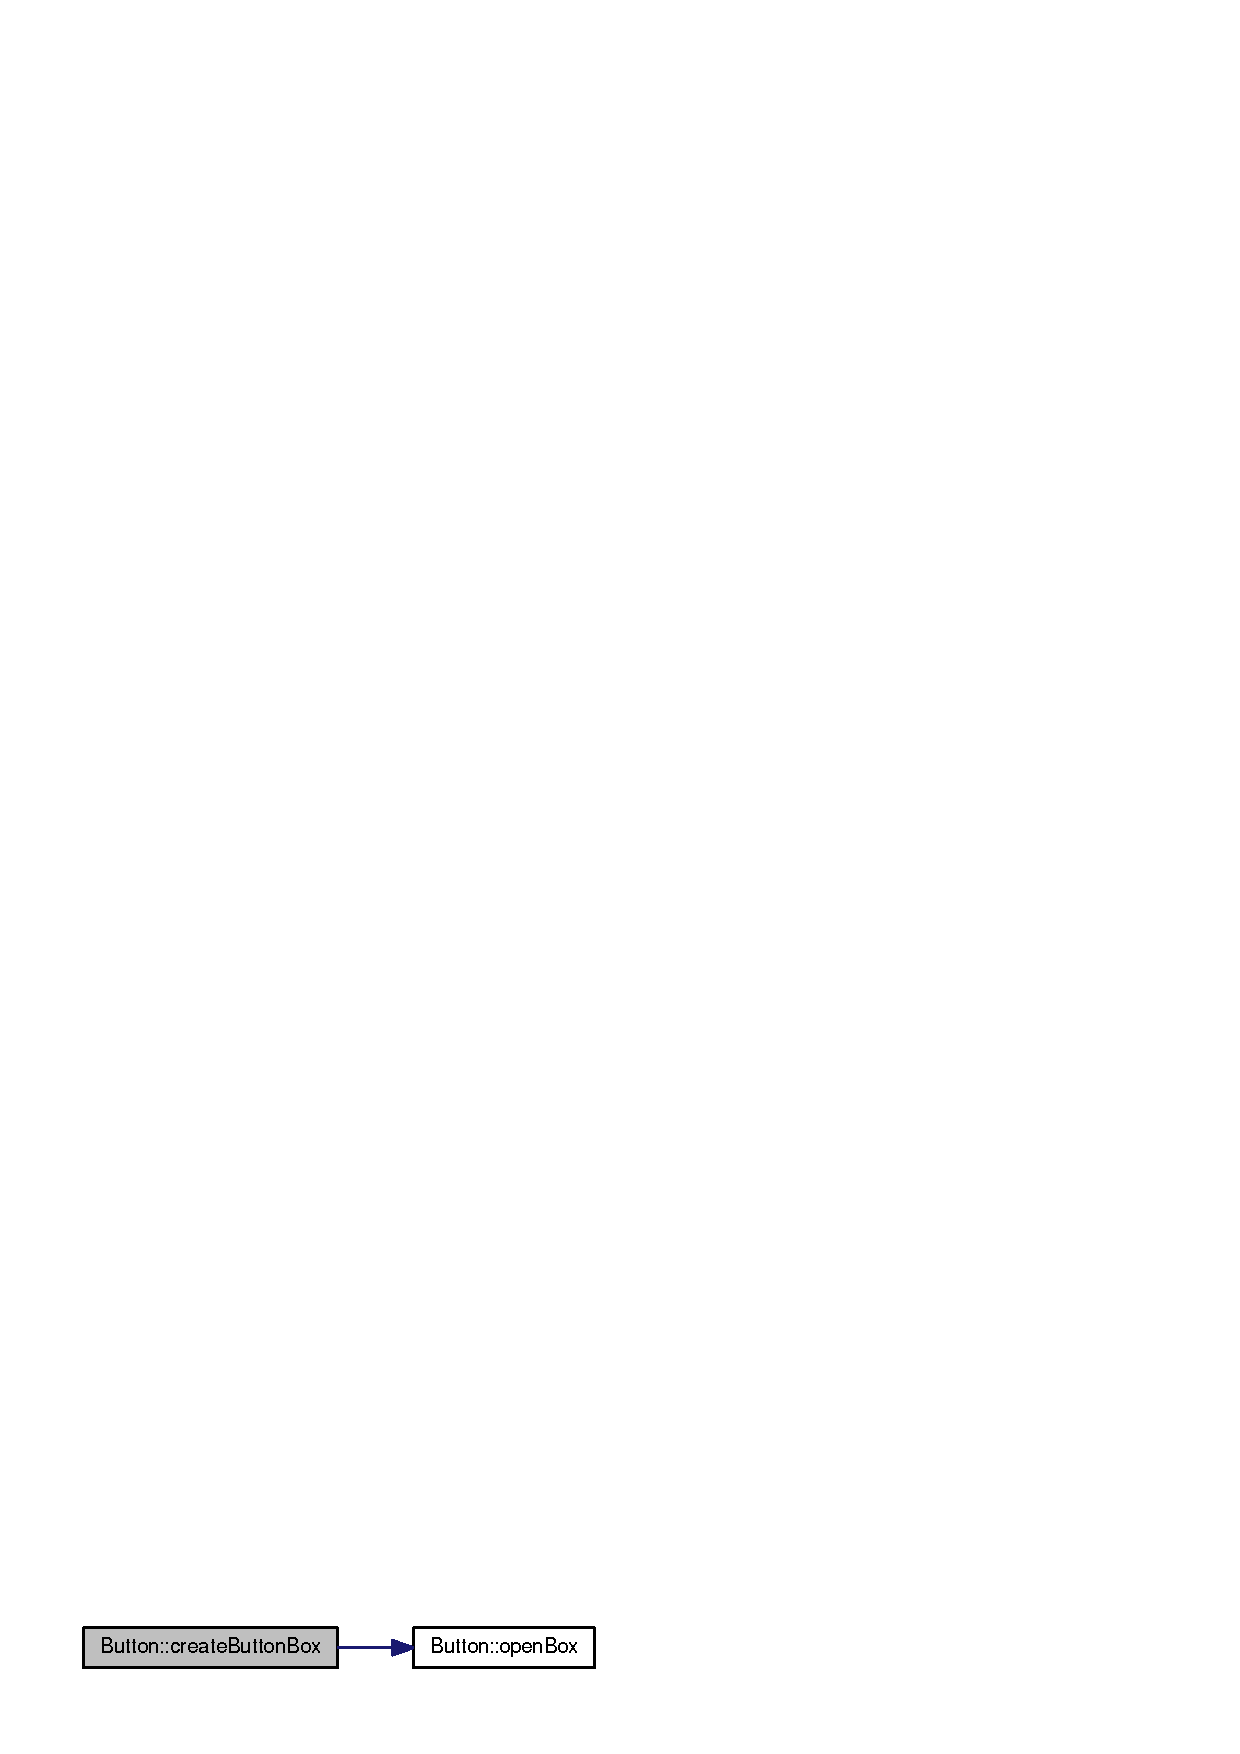
\includegraphics[width=290pt]{class_button_a10293cc4dcea650ad6b858430bb2a488_cgraph}
\end{center}
\end{figure}




Here is the caller graph for this function\-:\nopagebreak
\begin{figure}[H]
\begin{center}
\leavevmode
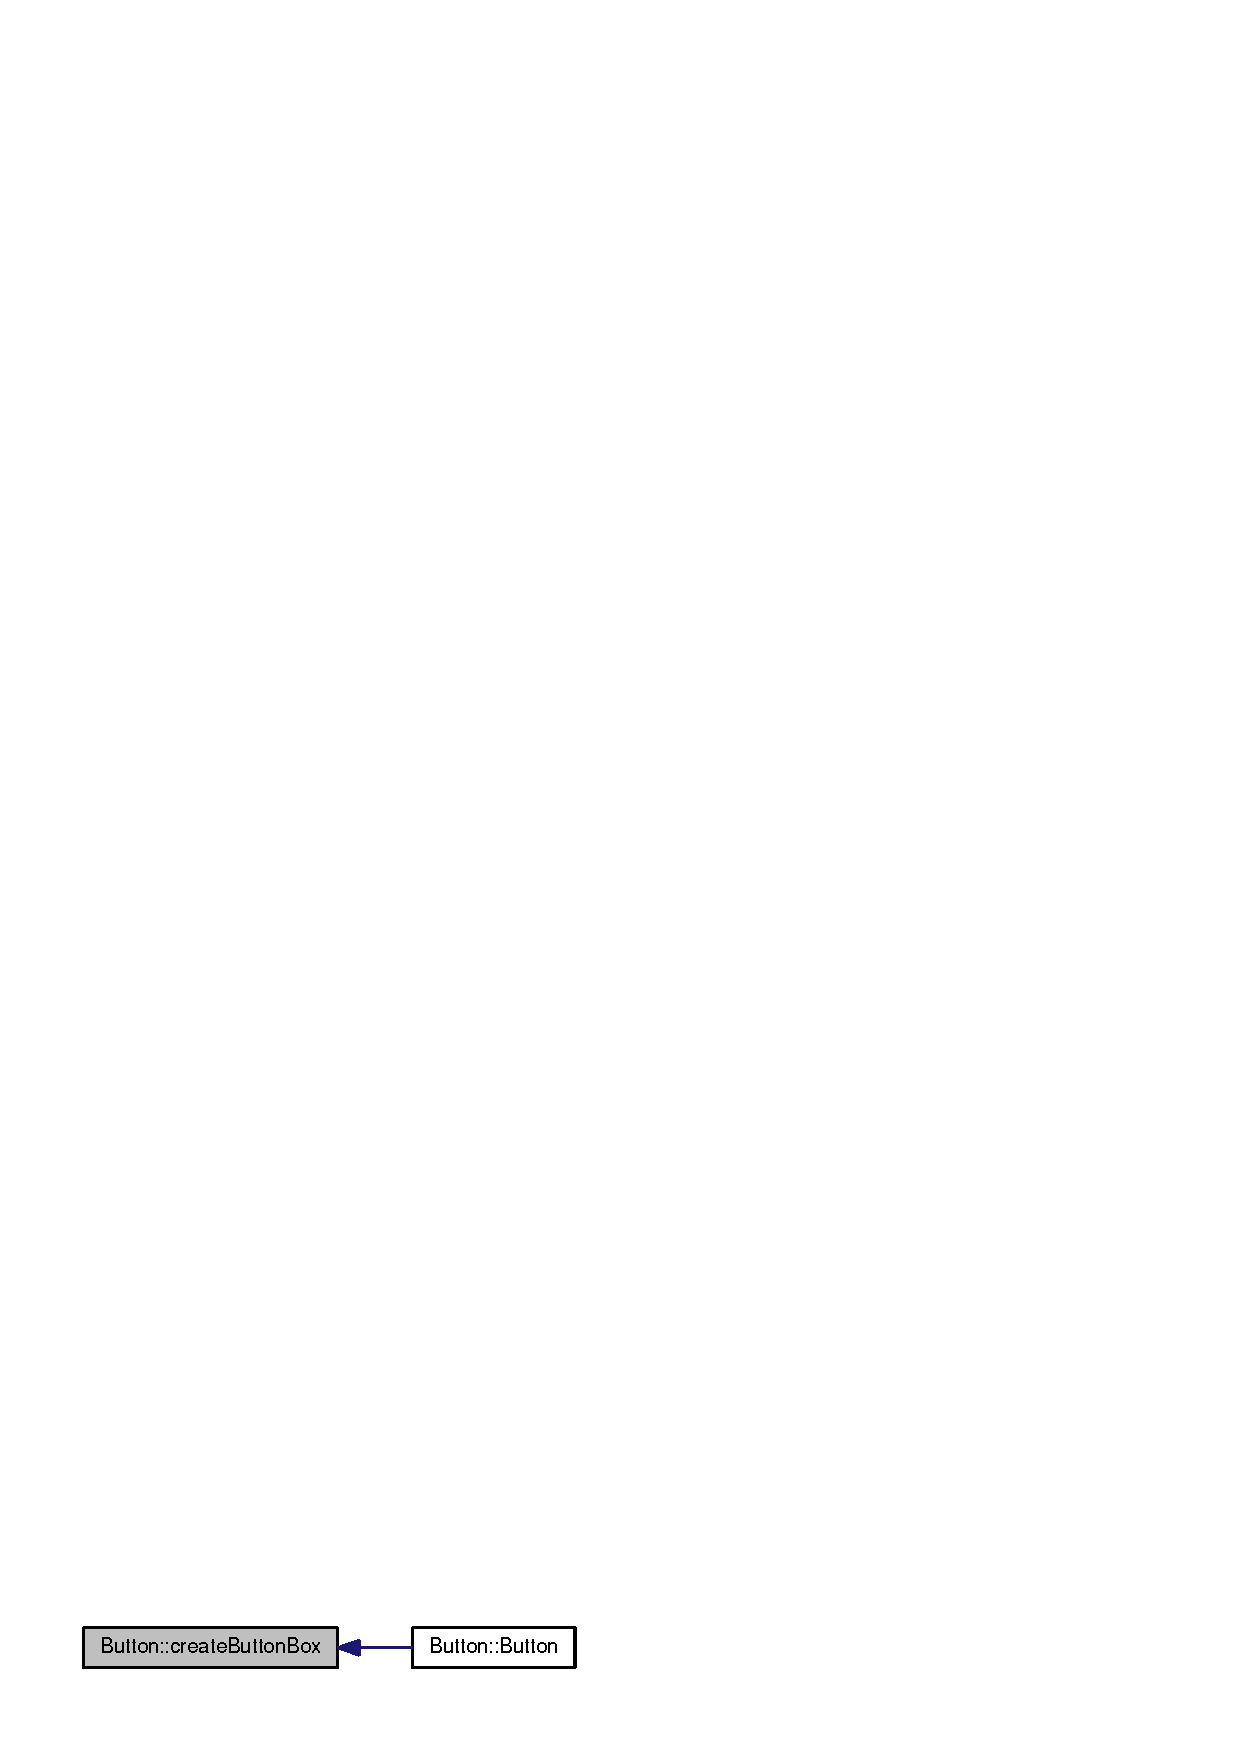
\includegraphics[width=280pt]{class_button_a10293cc4dcea650ad6b858430bb2a488_icgraph}
\end{center}
\end{figure}


\index{Button@{Button}!get\-Colour@{get\-Colour}}
\index{get\-Colour@{get\-Colour}!Button@{Button}}
\subsubsection[{get\-Colour}]{\setlength{\rightskip}{0pt plus 5cm}virtual ngl\-::\-Vec4 Button\-::get\-Colour (
\begin{DoxyParamCaption}
{}
\end{DoxyParamCaption}
)\hspace{0.3cm}{\ttfamily [inline]}, {\ttfamily [virtual]}}\label{class_button_a70975849d59dca023bd95047dfd0771e}


returns the colour, stored by the button 

\begin{DoxyReturn}{Returns}
m\-\_\-colour 
\end{DoxyReturn}


Reimplemented in {\bf Colour\-Button} \doxyref{}{p.}{class_colour_button_ab16ef6ea899d28e8b8a8500d95a5d188}.



Definition at line 121 of file Button.\-h.


\begin{DoxyCode}
121 \{\textcolor{keywordflow}{return} ngl::Vec4();\}
\end{DoxyCode}
\index{Button@{Button}!get\-Colour\-Q@{get\-Colour\-Q}}
\index{get\-Colour\-Q@{get\-Colour\-Q}!Button@{Button}}
\subsubsection[{get\-Colour\-Q}]{\setlength{\rightskip}{0pt plus 5cm}virtual Q\-Color Button\-::get\-Colour\-Q (
\begin{DoxyParamCaption}
{}
\end{DoxyParamCaption}
)\hspace{0.3cm}{\ttfamily [inline]}, {\ttfamily [virtual]}}\label{class_button_aca34c082733f62c47cee7e278b3ae876}


returns the Q\-Colour, stored by the button 

\begin{DoxyReturn}{Returns}
m\-\_\-colour 
\end{DoxyReturn}


Reimplemented in {\bf Colour\-Button} \doxyref{}{p.}{class_colour_button_a3063b9d295eb8f9f0a0f69726f2c9449}.



Definition at line 125 of file Button.\-h.


\begin{DoxyCode}
125 \{\textcolor{keywordflow}{return} QColor();\}
\end{DoxyCode}
\index{Button@{Button}!get\-I\-D@{get\-I\-D}}
\index{get\-I\-D@{get\-I\-D}!Button@{Button}}
\subsubsection[{get\-I\-D}]{\setlength{\rightskip}{0pt plus 5cm}G\-Luint Button\-::get\-I\-D (
\begin{DoxyParamCaption}
{}
\end{DoxyParamCaption}
)\hspace{0.3cm}{\ttfamily [inline]}}\label{class_button_acc98380319a334fba0eb04e3fcb022aa}


returns the button I\-D, this will change based on shader location 

\begin{DoxyReturn}{Returns}
m\-\_\-id 
\end{DoxyReturn}


Definition at line 106 of file Button.\-h.



References m\-\_\-id.


\begin{DoxyCode}
106 \{\textcolor{keywordflow}{return} m_id;\}
\end{DoxyCode}
\index{Button@{Button}!get\-Name@{get\-Name}}
\index{get\-Name@{get\-Name}!Button@{Button}}
\subsubsection[{get\-Name}]{\setlength{\rightskip}{0pt plus 5cm}Q\-String Button\-::get\-Name (
\begin{DoxyParamCaption}
{}
\end{DoxyParamCaption}
)\hspace{0.3cm}{\ttfamily [inline]}}\label{class_button_a3b2ba90ccc29decb2e75364bab067d40}


returns the current button name 

\begin{DoxyReturn}{Returns}
m\-\_\-button\-Name 
\end{DoxyReturn}


Definition at line 91 of file Button.\-h.



References m\-\_\-button\-Name.


\begin{DoxyCode}
91 \{\textcolor{keywordflow}{return} m_buttonName;\}
\end{DoxyCode}
\index{Button@{Button}!get\-Type\-Enum@{get\-Type\-Enum}}
\index{get\-Type\-Enum@{get\-Type\-Enum}!Button@{Button}}
\subsubsection[{get\-Type\-Enum}]{\setlength{\rightskip}{0pt plus 5cm}G\-Lenum Button\-::get\-Type\-Enum (
\begin{DoxyParamCaption}
{}
\end{DoxyParamCaption}
)\hspace{0.3cm}{\ttfamily [inline]}}\label{class_button_aa4937ca8b719215bd439908cb81ff2b4}


returns the current button type 

\begin{DoxyReturn}{Returns}
m\-\_\-button\-Type 
\end{DoxyReturn}


Definition at line 96 of file Button.\-h.



References m\-\_\-button\-Type.


\begin{DoxyCode}
96 \{\textcolor{keywordflow}{return} m_buttonType;\}
\end{DoxyCode}
\index{Button@{Button}!get\-Value@{get\-Value}}
\index{get\-Value@{get\-Value}!Button@{Button}}
\subsubsection[{get\-Value}]{\setlength{\rightskip}{0pt plus 5cm}virtual float Button\-::get\-Value (
\begin{DoxyParamCaption}
{}
\end{DoxyParamCaption}
)\hspace{0.3cm}{\ttfamily [inline]}, {\ttfamily [virtual]}}\label{class_button_a324f19659d882f3a505a128dab9473e6}


returns the value, stored by the button 

\begin{DoxyReturn}{Returns}
m\-\_\-value 
\end{DoxyReturn}


Reimplemented in {\bf Float\-Button} \doxyref{}{p.}{class_float_button_ae83f81998a5ad1cff31bdb4a0a9250fd}.



Definition at line 135 of file Button.\-h.


\begin{DoxyCode}
135 \{\textcolor{keywordflow}{return} float();\}
\end{DoxyCode}
\index{Button@{Button}!get\-Vec@{get\-Vec}}
\index{get\-Vec@{get\-Vec}!Button@{Button}}
\subsubsection[{get\-Vec}]{\setlength{\rightskip}{0pt plus 5cm}virtual ngl\-::\-Vec4 Button\-::get\-Vec (
\begin{DoxyParamCaption}
{}
\end{DoxyParamCaption}
)\hspace{0.3cm}{\ttfamily [inline]}, {\ttfamily [virtual]}}\label{class_button_a5d3781edfd3746dcc604737cf6e5cbf2}


returns the Vec4 held by the vector button class 

\begin{DoxyReturn}{Returns}
m\-\_\-value 
\end{DoxyReturn}


Reimplemented in {\bf Vec\-Button} \doxyref{}{p.}{class_vec_button_a41dbe6736fcc2ff329accae19bd9657f}.



Definition at line 144 of file Button.\-h.


\begin{DoxyCode}
144 \{\textcolor{keywordflow}{return} ngl::Vec4();\}
\end{DoxyCode}
\index{Button@{Button}!open\-Box@{open\-Box}}
\index{open\-Box@{open\-Box}!Button@{Button}}
\subsubsection[{open\-Box}]{\setlength{\rightskip}{0pt plus 5cm}virtual void Button\-::open\-Box (
\begin{DoxyParamCaption}
{}
\end{DoxyParamCaption}
)\hspace{0.3cm}{\ttfamily [inline]}, {\ttfamily [private]}, {\ttfamily [virtual]}, {\ttfamily [slot]}}\label{class_button_a9744bb5db7d847384e243ba5f4bad1d8}


a slot to open a widget upon button press event 



Definition at line 183 of file Button.\-h.


\begin{DoxyCode}
183 \{\textcolor{keywordflow}{return};\}
\end{DoxyCode}


Here is the caller graph for this function\-:\nopagebreak
\begin{figure}[H]
\begin{center}
\leavevmode
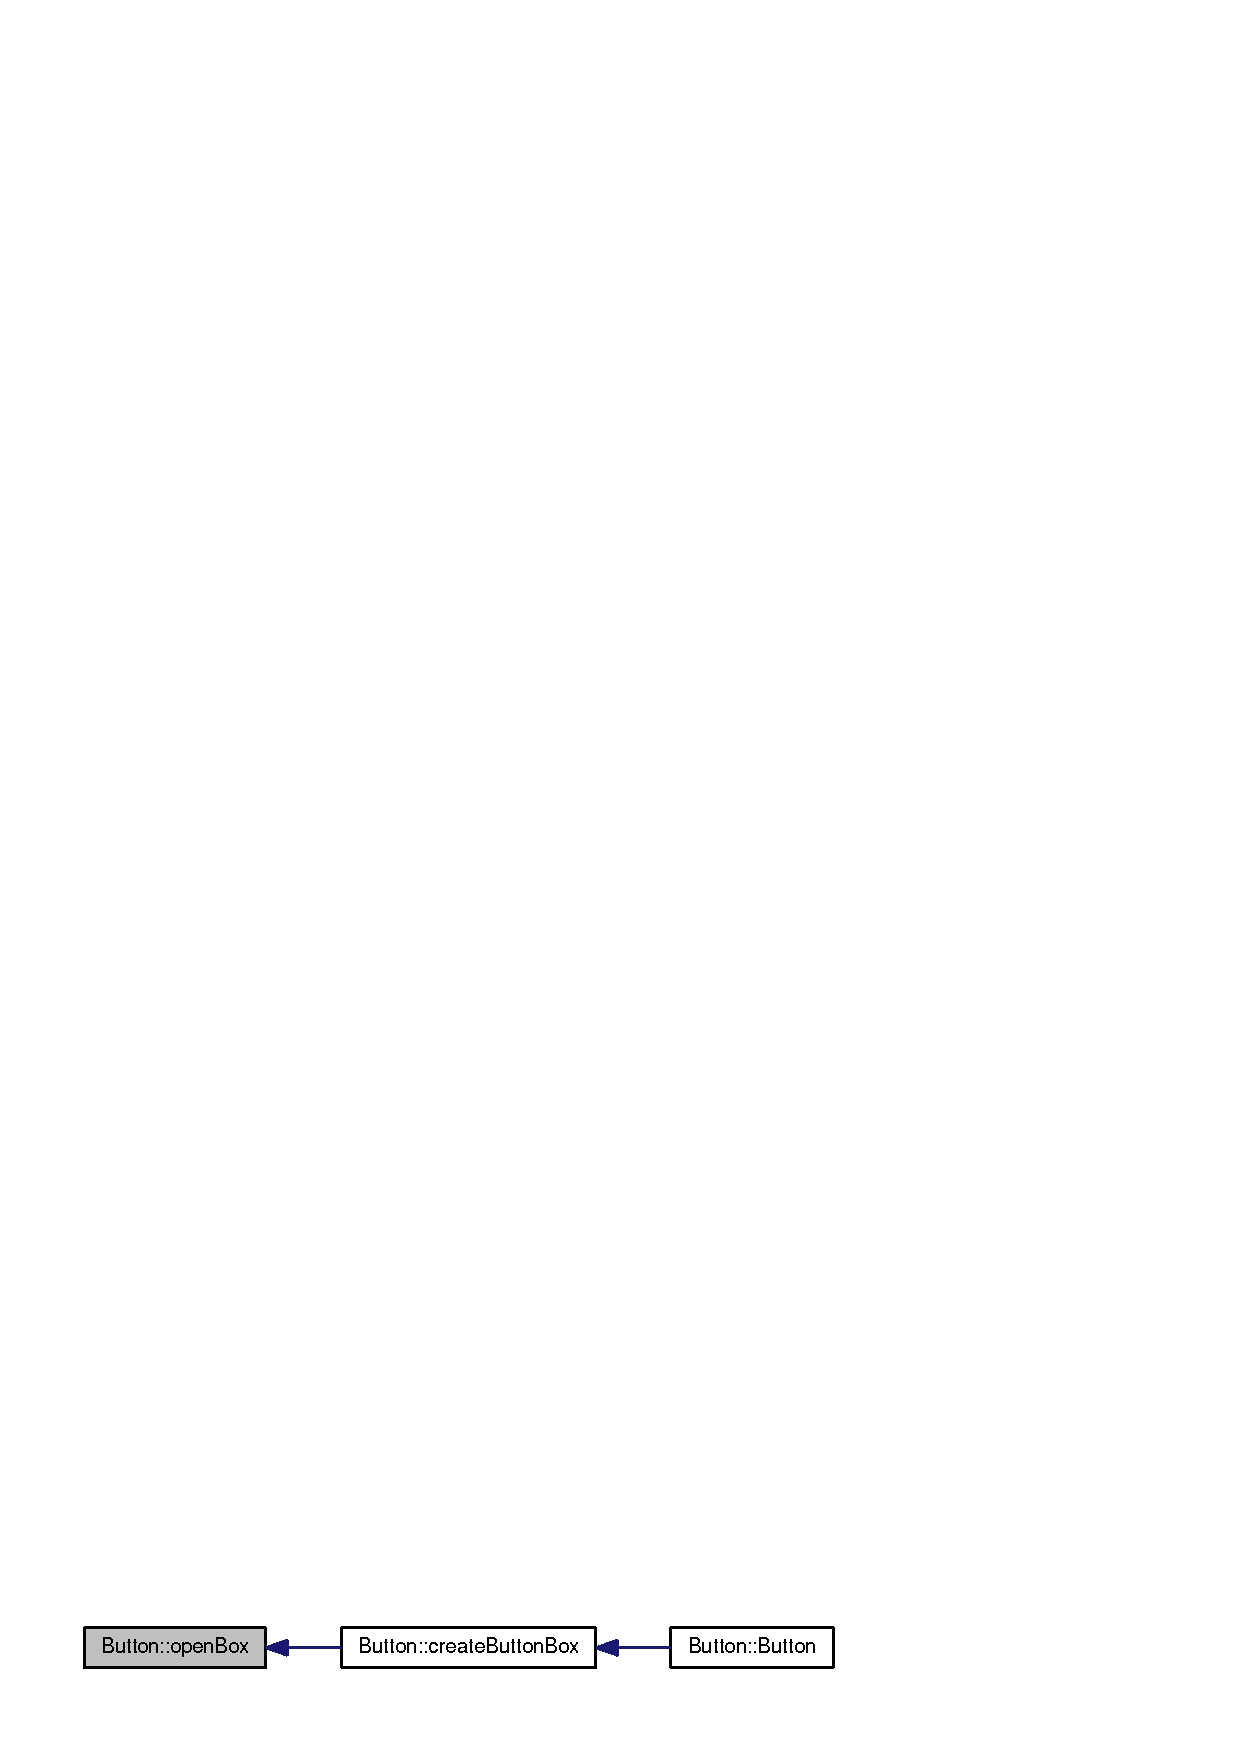
\includegraphics[width=350pt]{class_button_a9744bb5db7d847384e243ba5f4bad1d8_icgraph}
\end{center}
\end{figure}


\index{Button@{Button}!print\-Values@{print\-Values}}
\index{print\-Values@{print\-Values}!Button@{Button}}
\subsubsection[{print\-Values}]{\setlength{\rightskip}{0pt plus 5cm}void Button\-::print\-Values (
\begin{DoxyParamCaption}
{}
\end{DoxyParamCaption}
)\hspace{0.3cm}{\ttfamily [virtual]}}\label{class_button_a9821ae14c606648a3dcd195714e30f3c}


prints the button attribute values 



Definition at line 37 of file Button.\-cpp.



References m\-\_\-button\-Name, and m\-\_\-id.


\begin{DoxyCode}
38 \{
39   qDebug()<<\textcolor{stringliteral}{"Name:"}<<m_buttonName<<\textcolor{stringliteral}{"\(\backslash\)nID: "}<<m_id;
40 \}
\end{DoxyCode}
\index{Button@{Button}!set\-Colour@{set\-Colour}}
\index{set\-Colour@{set\-Colour}!Button@{Button}}
\subsubsection[{set\-Colour}]{\setlength{\rightskip}{0pt plus 5cm}virtual void Button\-::set\-Colour (
\begin{DoxyParamCaption}
\item[{ngl\-::\-Vec4}]{\-\_\-col}
\end{DoxyParamCaption}
)\hspace{0.3cm}{\ttfamily [inline]}, {\ttfamily [virtual]}}\label{class_button_a339347e88020f2c961e08a530407d083}


sets the colour to be used by colour buttons 


\begin{DoxyParams}[1]{Parameters}
\mbox{\tt in}  & {\em the} & colour to be set within the colour\-Button class \\
\hline
\end{DoxyParams}


Reimplemented in {\bf Colour\-Button} \doxyref{}{p.}{class_colour_button_abb4011f8d6d85856a2ee155817b52135}.



Definition at line 111 of file Button.\-h.


\begin{DoxyCode}
111 \{\textcolor{keywordflow}{return};\}
\end{DoxyCode}
\index{Button@{Button}!set\-Colour@{set\-Colour}}
\index{set\-Colour@{set\-Colour}!Button@{Button}}
\subsubsection[{set\-Colour}]{\setlength{\rightskip}{0pt plus 5cm}virtual void Button\-::set\-Colour (
\begin{DoxyParamCaption}
\item[{Q\-Color}]{\-\_\-col}
\end{DoxyParamCaption}
)\hspace{0.3cm}{\ttfamily [inline]}, {\ttfamily [virtual]}}\label{class_button_a174b05c6f309a46db10530052cf8388a}


overloaded function to set the colour 


\begin{DoxyParams}[1]{Parameters}
\mbox{\tt in}  & {\em the} & colour to be set within the colour\-Button class \\
\hline
\end{DoxyParams}


Reimplemented in {\bf Colour\-Button} \doxyref{}{p.}{class_colour_button_a1702284d1cdfe7bff2db19e219132f37}.



Definition at line 116 of file Button.\-h.


\begin{DoxyCode}
116 \{\textcolor{keywordflow}{return};\}
\end{DoxyCode}
\index{Button@{Button}!set\-I\-D@{set\-I\-D}}
\index{set\-I\-D@{set\-I\-D}!Button@{Button}}
\subsubsection[{set\-I\-D}]{\setlength{\rightskip}{0pt plus 5cm}void Button\-::set\-I\-D (
\begin{DoxyParamCaption}
\item[{unsigned int}]{\-\_\-id}
\end{DoxyParamCaption}
)\hspace{0.3cm}{\ttfamily [inline]}}\label{class_button_a96d07509fe660457624a9d5b00d139e6}


sets the current I\-D for the button, from its' shader location 


\begin{DoxyParams}[1]{Parameters}
\mbox{\tt in}  & {\em the} & location I\-D for the button id \\
\hline
\end{DoxyParams}


Definition at line 101 of file Button.\-h.



References m\-\_\-id.


\begin{DoxyCode}
101 \{m_id=\_id;\}
\end{DoxyCode}
\index{Button@{Button}!set\-Value@{set\-Value}}
\index{set\-Value@{set\-Value}!Button@{Button}}
\subsubsection[{set\-Value}]{\setlength{\rightskip}{0pt plus 5cm}virtual void Button\-::set\-Value (
\begin{DoxyParamCaption}
\item[{float}]{\-\_\-val}
\end{DoxyParamCaption}
)\hspace{0.3cm}{\ttfamily [inline]}, {\ttfamily [virtual]}}\label{class_button_aac9f26f6c9a02dd1c9dfa47c71b0495d}


sets the value to be for float attributes 


\begin{DoxyParams}[1]{Parameters}
\mbox{\tt in}  & {\em the} & value to be set within the float\-Button class \\
\hline
\end{DoxyParams}


Reimplemented in {\bf Float\-Button} \doxyref{}{p.}{class_float_button_a7878ecb2411a54c76e297f0988bfef6a}.



Definition at line 130 of file Button.\-h.


\begin{DoxyCode}
130 \{\textcolor{keywordflow}{return};\}
\end{DoxyCode}
\index{Button@{Button}!set\-Vec@{set\-Vec}}
\index{set\-Vec@{set\-Vec}!Button@{Button}}
\subsubsection[{set\-Vec}]{\setlength{\rightskip}{0pt plus 5cm}virtual void Button\-::set\-Vec (
\begin{DoxyParamCaption}
\item[{ngl\-::\-Vec4}]{\-\_\-value}
\end{DoxyParamCaption}
)\hspace{0.3cm}{\ttfamily [inline]}, {\ttfamily [virtual]}}\label{class_button_a796b8d995b90901474020afe94db2670}


sets the vector value for Vec3s or positions 


\begin{DoxyParams}[1]{Parameters}
\mbox{\tt in}  & {\em \-\_\-value} & to be set within the \doxyref{Vec\-Button}{p.}{class_vec_button} class \\
\hline
\end{DoxyParams}


Reimplemented in {\bf Vec\-Button} \doxyref{}{p.}{class_vec_button_ad6031636201b20b40bdab28e90a4f427}.



Definition at line 149 of file Button.\-h.


\begin{DoxyCode}
149 \{\textcolor{keywordflow}{return};\}
\end{DoxyCode}


\subsection{Member Data Documentation}
\index{Button@{Button}!m\-\_\-button@{m\-\_\-button}}
\index{m\-\_\-button@{m\-\_\-button}!Button@{Button}}
\subsubsection[{m\-\_\-button}]{\setlength{\rightskip}{0pt plus 5cm}Q\-Push\-Button$\ast$ Button\-::m\-\_\-button}\label{class_button_a4b94df529b727db6a5855159f2e7b46b}


button object to be pressed by user to open relevant widget 



Definition at line 67 of file Button.\-h.

\index{Button@{Button}!m\-\_\-button\-Box@{m\-\_\-button\-Box}}
\index{m\-\_\-button\-Box@{m\-\_\-button\-Box}!Button@{Button}}
\subsubsection[{m\-\_\-button\-Box}]{\setlength{\rightskip}{0pt plus 5cm}Q\-Dialog\-Button\-Box$\ast$ Button\-::m\-\_\-button\-Box\hspace{0.3cm}{\ttfamily [private]}}\label{class_button_a799f1a86591ad30d77c91682d4b17d0f}


button box used to activate the opening of the widget 



Definition at line 167 of file Button.\-h.

\index{Button@{Button}!m\-\_\-button\-Name@{m\-\_\-button\-Name}}
\index{m\-\_\-button\-Name@{m\-\_\-button\-Name}!Button@{Button}}
\subsubsection[{m\-\_\-button\-Name}]{\setlength{\rightskip}{0pt plus 5cm}Q\-String Button\-::m\-\_\-button\-Name\hspace{0.3cm}{\ttfamily [private]}}\label{class_button_a8709a2ba9cc9c26c44e34920cec1e10c}


string to hold button's name 



Definition at line 155 of file Button.\-h.

\index{Button@{Button}!m\-\_\-button\-Type@{m\-\_\-button\-Type}}
\index{m\-\_\-button\-Type@{m\-\_\-button\-Type}!Button@{Button}}
\subsubsection[{m\-\_\-button\-Type}]{\setlength{\rightskip}{0pt plus 5cm}G\-Lenum Button\-::m\-\_\-button\-Type\hspace{0.3cm}{\ttfamily [private]}}\label{class_button_af796dcbe5e14a93916cc8be1d6fd2c0e}


enum for the button type, used for defining type 



Definition at line 159 of file Button.\-h.

\index{Button@{Button}!m\-\_\-grid\-Layout@{m\-\_\-grid\-Layout}}
\index{m\-\_\-grid\-Layout@{m\-\_\-grid\-Layout}!Button@{Button}}
\subsubsection[{m\-\_\-grid\-Layout}]{\setlength{\rightskip}{0pt plus 5cm}Q\-Grid\-Layout$\ast$ Button\-::m\-\_\-grid\-Layout\hspace{0.3cm}{\ttfamily [private]}}\label{class_button_a601e932697cae4bbe108b14fac80cd1a}


layout for the button box to be stored within 



Definition at line 171 of file Button.\-h.

\index{Button@{Button}!m\-\_\-id@{m\-\_\-id}}
\index{m\-\_\-id@{m\-\_\-id}!Button@{Button}}
\subsubsection[{m\-\_\-id}]{\setlength{\rightskip}{0pt plus 5cm}unsigned int Button\-::m\-\_\-id\hspace{0.3cm}{\ttfamily [private]}}\label{class_button_a57231848f1cddc86a85cdb01a8e41ed2}


id to access specific buttons and shader locations 



Definition at line 163 of file Button.\-h.

\index{Button@{Button}!m\-\_\-lib\-Parent@{m\-\_\-lib\-Parent}}
\index{m\-\_\-lib\-Parent@{m\-\_\-lib\-Parent}!Button@{Button}}
\subsubsection[{m\-\_\-lib\-Parent}]{\setlength{\rightskip}{0pt plus 5cm}{\bf Button\-Lib}$\ast$ Button\-::m\-\_\-lib\-Parent}\label{class_button_a5ffdc2d1347d0633328e03801ee9ce69}


pointer to the button library parent 



Definition at line 55 of file Button.\-h.

\index{Button@{Button}!m\-\_\-parent@{m\-\_\-parent}}
\index{m\-\_\-parent@{m\-\_\-parent}!Button@{Button}}
\subsubsection[{m\-\_\-parent}]{\setlength{\rightskip}{0pt plus 5cm}Q\-Widget$\ast$ Button\-::m\-\_\-parent}\label{class_button_a4e649c5f7b62db1da6a57467e743b1b5}


pointer to the parent window to know where to attach to 



Definition at line 63 of file Button.\-h.

\index{Button@{Button}!m\-\_\-scene\-Parent@{m\-\_\-scene\-Parent}}
\index{m\-\_\-scene\-Parent@{m\-\_\-scene\-Parent}!Button@{Button}}
\subsubsection[{m\-\_\-scene\-Parent}]{\setlength{\rightskip}{0pt plus 5cm}{\bf N\-G\-L\-Scene}$\ast$ Button\-::m\-\_\-scene\-Parent}\label{class_button_aa3ce7a1873a2d1b14d05e6381b900fb7}


pointer to the scene so that update can be called 



Definition at line 59 of file Button.\-h.



The documentation for this class was generated from the following files\-:\begin{DoxyCompactItemize}
\item 
{\bf Button.\-h}\item 
{\bf Button.\-cpp}\end{DoxyCompactItemize}

\section{Button\-Lib Class Reference}
\label{class_button_lib}\index{Button\-Lib@{Button\-Lib}}


Stores vector of buttons with values and updates uniforms.  




{\ttfamily \#include $<$Button\-Lib.\-h$>$}



Collaboration diagram for Button\-Lib\-:\nopagebreak
\begin{figure}[H]
\begin{center}
\leavevmode
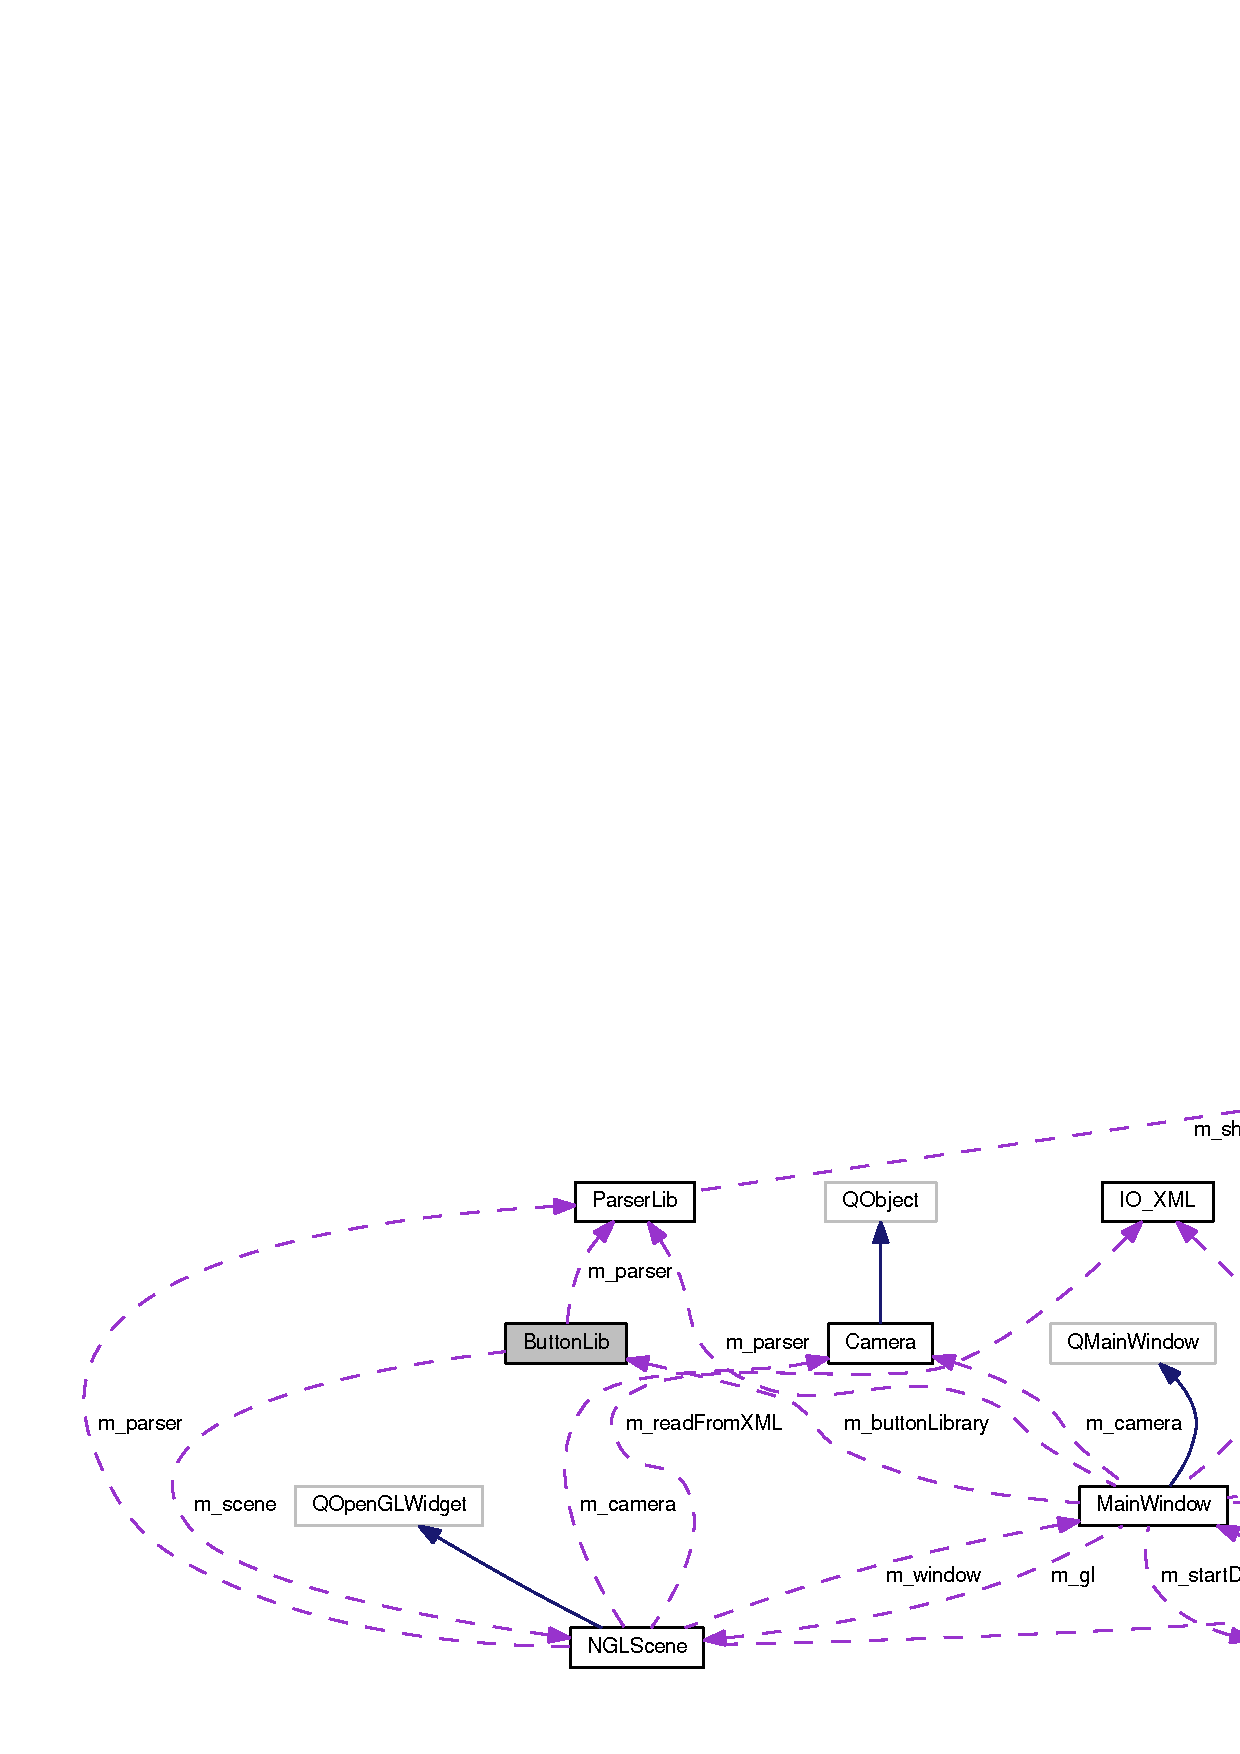
\includegraphics[width=350pt]{class_button_lib__coll__graph}
\end{center}
\end{figure}
\subsection*{Public Member Functions}
\begin{DoxyCompactItemize}
\item 
{\bf Button\-Lib} ({\bf Parser\-Lib} $\ast$\-\_\-parser, Q\-Layout $\ast$\-\_\-layout, {\bf N\-G\-L\-Scene} $\ast$\-\_\-scene, Q\-Widget $\ast$\-\_\-parent=0)
\begin{DoxyCompactList}\small\item\em constructor to create the button library \end{DoxyCompactList}\item 
void {\bf create\-Buttons} ()
\begin{DoxyCompactList}\small\item\em call to a function to create the buttons in the gui \end{DoxyCompactList}\item 
void {\bf update\-Buttons} ()
\begin{DoxyCompactList}\small\item\em call to update the buttons \end{DoxyCompactList}\item 
void {\bf print\-Uniforms} ()
\begin{DoxyCompactList}\small\item\em prints the uniforms for debugging purposes \end{DoxyCompactList}\item 
void {\bf update\-Shader\-Values} ()
\begin{DoxyCompactList}\small\item\em sets the shader values from the button values \end{DoxyCompactList}\end{DoxyCompactItemize}
\subsection*{Private Attributes}
\begin{DoxyCompactItemize}
\item 
Q\-Layout $\ast$ {\bf m\-\_\-layout}
\begin{DoxyCompactList}\small\item\em gui layout for the buttons to be stored in \end{DoxyCompactList}\item 
Q\-Widget $\ast$ {\bf m\-\_\-parent}
\begin{DoxyCompactList}\small\item\em gui parent for the layout \end{DoxyCompactList}\item 
{\bf Parser\-Lib} $\ast$ {\bf m\-\_\-parser}
\begin{DoxyCompactList}\small\item\em pointer to the parser to access and set uniform values \end{DoxyCompactList}\item 
{\bf N\-G\-L\-Scene} $\ast$ {\bf m\-\_\-scene}
\begin{DoxyCompactList}\small\item\em pointer to the \doxyref{N\-G\-L\-Scene}{p.}{class_n_g_l_scene}, gl Widget \end{DoxyCompactList}\item 
std\-::vector$<$ {\bf Button} $\ast$ $>$ {\bf m\-\_\-button\-List}
\begin{DoxyCompactList}\small\item\em vector of buttons to dynamically and delete different types \end{DoxyCompactList}\end{DoxyCompactItemize}


\subsection{Detailed Description}
Stores vector of buttons with values and updates uniforms. 

Definition at line 25 of file Button\-Lib.\-h.



\subsection{Constructor \& Destructor Documentation}
\index{Button\-Lib@{Button\-Lib}!Button\-Lib@{Button\-Lib}}
\index{Button\-Lib@{Button\-Lib}!ButtonLib@{Button\-Lib}}
\subsubsection[{Button\-Lib}]{\setlength{\rightskip}{0pt plus 5cm}Button\-Lib\-::\-Button\-Lib (
\begin{DoxyParamCaption}
\item[{{\bf Parser\-Lib} $\ast$}]{\-\_\-parser, }
\item[{Q\-Layout $\ast$}]{\-\_\-layout, }
\item[{{\bf N\-G\-L\-Scene} $\ast$}]{\-\_\-scene, }
\item[{Q\-Widget $\ast$}]{\-\_\-parent = {\ttfamily 0}}
\end{DoxyParamCaption}
)}\label{class_button_lib_aac3bfeb47972aa42c950c8bd0d4c69a5}


constructor to create the button library 


\begin{DoxyParams}[1]{Parameters}
\mbox{\tt in}  & {\em \-\_\-parser} & the parser to check and set uniforms \\
\hline
\mbox{\tt in}  & {\em \-\_\-layout} & the layout environment for the buttons to be attached to \\
\hline
\mbox{\tt in}  & {\em \-\_\-scene} & the \doxyref{N\-G\-L\-Scene}{p.}{class_n_g_l_scene} for the G\-U\-I \\
\hline
\mbox{\tt in}  & {\em \-\_\-parent} & the parent window for the buttons \\
\hline
\end{DoxyParams}


Definition at line 3 of file Button\-Lib.\-cpp.



References create\-Buttons(), m\-\_\-layout, m\-\_\-parent, m\-\_\-parser, m\-\_\-scene, and update\-Shader\-Values().


\begin{DoxyCode}
4 \{
5   m_parser=\_parser;
6   m_layout=\_layout;
7   m_parent=\_parent;
8   m_scene=\_scene;
9   createButtons();
10   updateShaderValues();
11 \}
\end{DoxyCode}


Here is the call graph for this function\-:\nopagebreak
\begin{figure}[H]
\begin{center}
\leavevmode
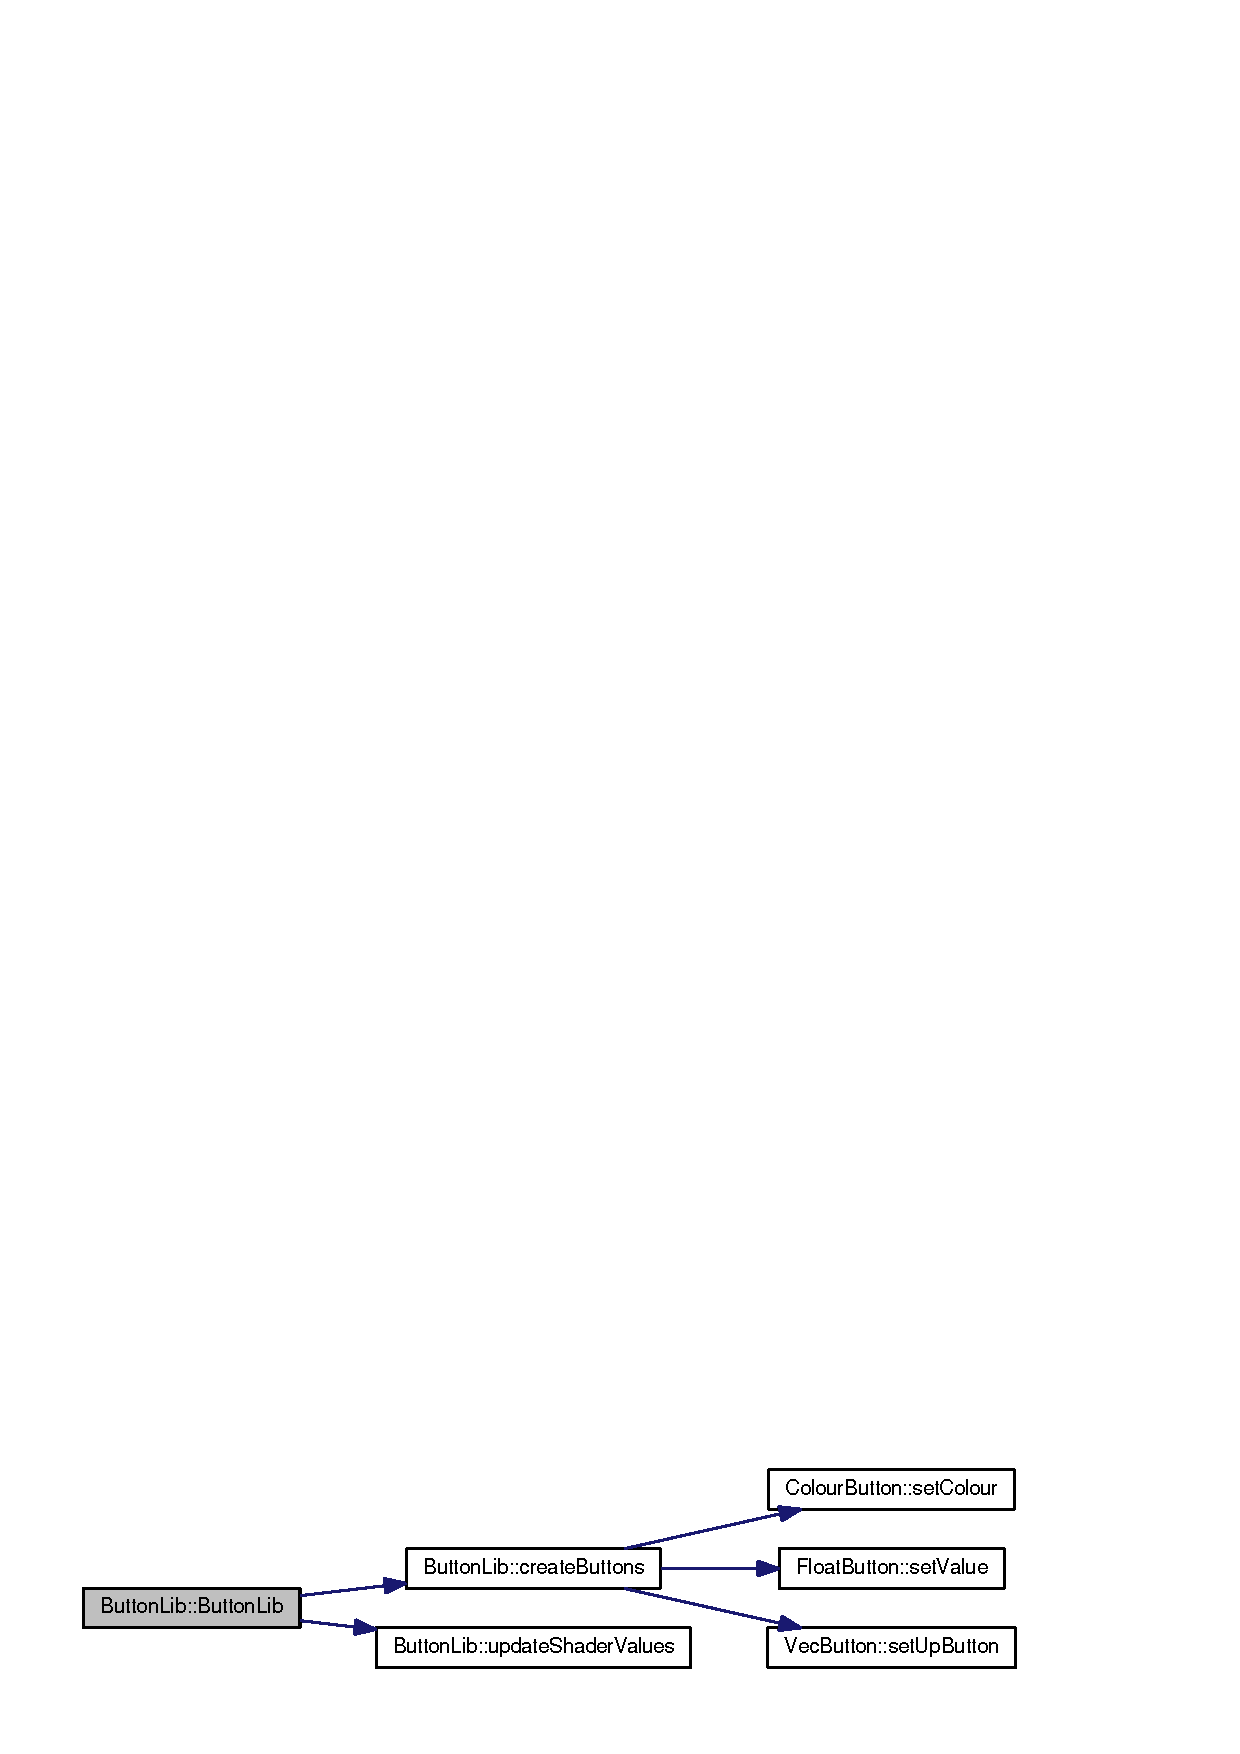
\includegraphics[width=350pt]{class_button_lib_aac3bfeb47972aa42c950c8bd0d4c69a5_cgraph}
\end{center}
\end{figure}




\subsection{Member Function Documentation}
\index{Button\-Lib@{Button\-Lib}!create\-Buttons@{create\-Buttons}}
\index{create\-Buttons@{create\-Buttons}!ButtonLib@{Button\-Lib}}
\subsubsection[{create\-Buttons}]{\setlength{\rightskip}{0pt plus 5cm}void Button\-Lib\-::create\-Buttons (
\begin{DoxyParamCaption}
{}
\end{DoxyParamCaption}
)}\label{class_button_lib_a88d97d584a95e601067ec420c4380f2d}


call to a function to create the buttons in the gui 



Definition at line 13 of file Button\-Lib.\-cpp.



References m\-\_\-button\-List, m\-\_\-layout, m\-\_\-parent, m\-\_\-parser, m\-\_\-scene, Parser\-Lib\-::m\-\_\-uniform\-List, Colour\-Button\-::set\-Colour(), Vec\-Button\-::set\-Up\-Button(), and Float\-Button\-::set\-Value().


\begin{DoxyCode}
14 \{
15   \textcolor{keywordflow}{for}(\textcolor{keyword}{auto} uniform : m_parser->m_uniformList)
16   \{
17     QString \_uniformName = QString::fromStdString(uniform->getName());
18     GLenum \_uniformType = uniform->getTypeEnum();
19     \textcolor{keywordflow}{if}(\_uniformType==GL\_FLOAT\_VEC4)
20     \{
21       ngl::Vec4 \_uniformVec=uniform->getVec4();
22       ColourButton *tempButton = \textcolor{keyword}{new} ColourButton(\_uniformName,
23                                                   \_uniformType,
24                                                   m_layout,
25                                                   uniform->getLocation(),
26                                                   \textcolor{keyword}{this},
27                                                   m_scene,
28                                                   m_parent);
29       tempButton->setColour(\_uniformVec);
30       m_buttonList.push\_back(tempButton);
31     \}
32     \textcolor{keywordflow}{if}(\_uniformType==GL\_FLOAT)
33     \{
34       \textcolor{keywordtype}{float} \_uniformFloat=uniform->getFloat();
35       FloatButton *tempButton = \textcolor{keyword}{new} FloatButton(\_uniformName,
36                                                 \_uniformType,
37                                                 m_layout,
38                                                 uniform->getLocation(),
39                                                 \textcolor{keyword}{this},
40                                                 m_scene,
41                                                 m_parent);
42       tempButton->setValue(\_uniformFloat);
43       m_buttonList.push\_back(tempButton);
44     \}
45     \textcolor{keywordflow}{if}(\_uniformType==GL\_FLOAT\_VEC3)
46     \{
47       ngl::Vec3 \_uniformVec=uniform->getVec3();
48       VecButton *tempButton = \textcolor{keyword}{new} VecButton(\_uniformName,
49                                                   \_uniformType,
50                                                   m_layout,
51                                                   uniform->getLocation(),
52                                                   \textcolor{keyword}{this},
53                                                   m_scene,
54                                                   m_parent);
55       tempButton->setUpButton(\_uniformVec);
56       m_buttonList.push\_back(tempButton);
57     \}
58   \}
59 \}
\end{DoxyCode}


Here is the call graph for this function\-:\nopagebreak
\begin{figure}[H]
\begin{center}
\leavevmode
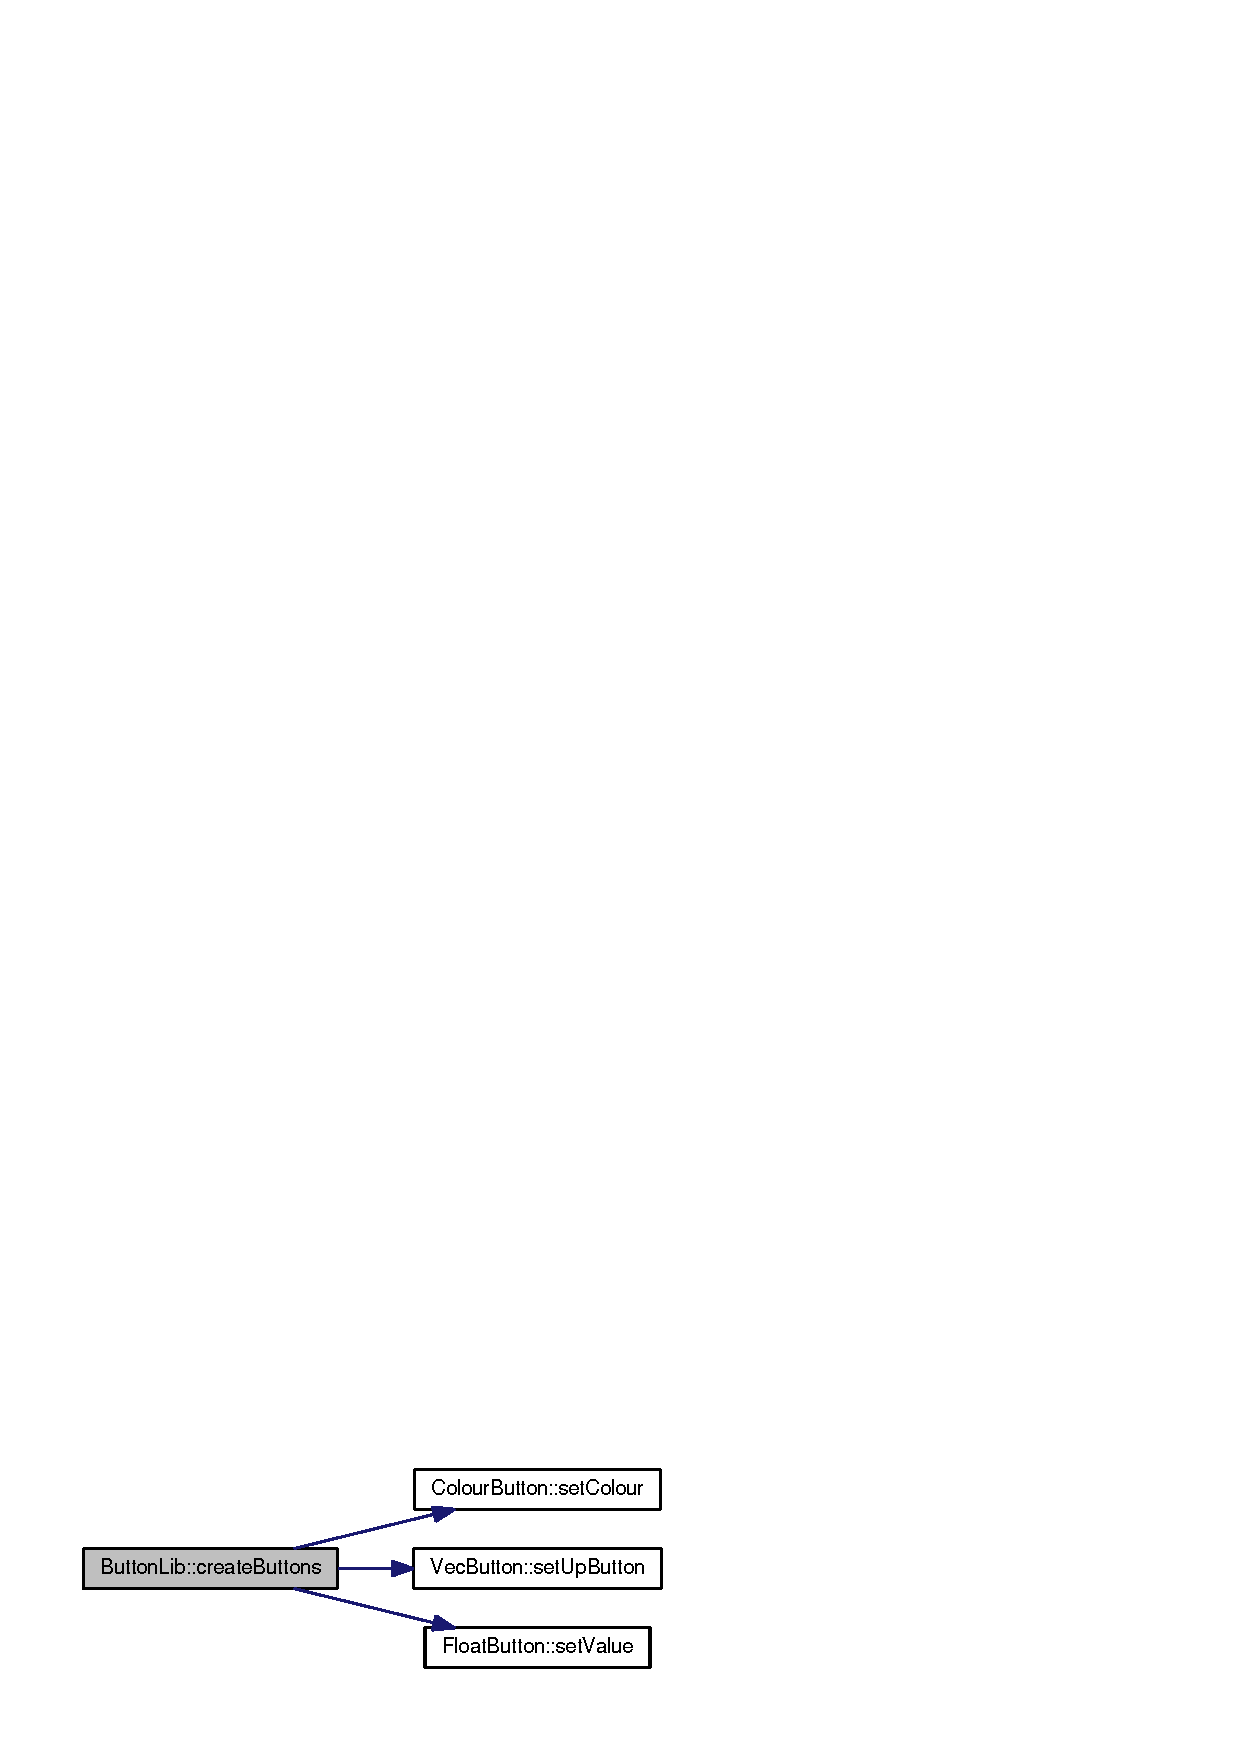
\includegraphics[width=322pt]{class_button_lib_a88d97d584a95e601067ec420c4380f2d_cgraph}
\end{center}
\end{figure}




Here is the caller graph for this function\-:\nopagebreak
\begin{figure}[H]
\begin{center}
\leavevmode
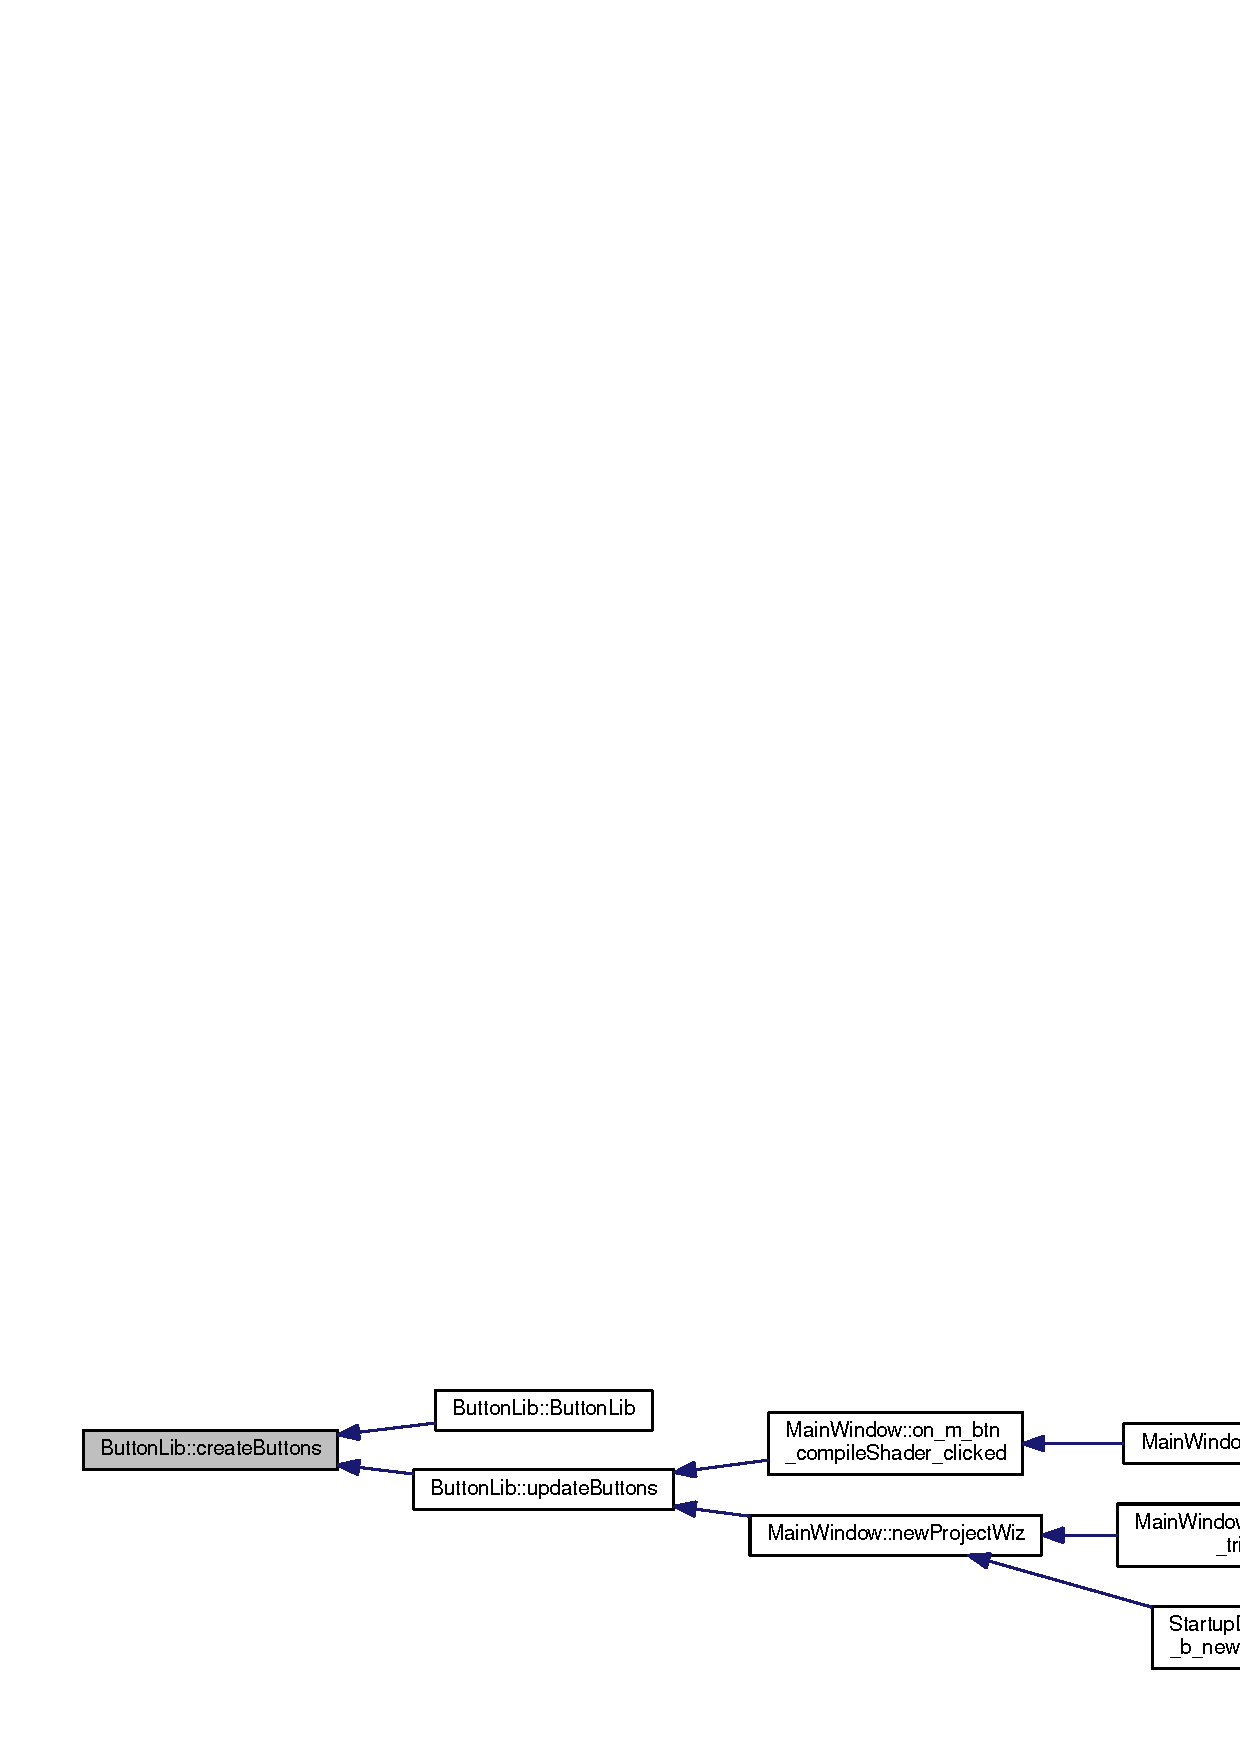
\includegraphics[width=350pt]{class_button_lib_a88d97d584a95e601067ec420c4380f2d_icgraph}
\end{center}
\end{figure}


\index{Button\-Lib@{Button\-Lib}!print\-Uniforms@{print\-Uniforms}}
\index{print\-Uniforms@{print\-Uniforms}!ButtonLib@{Button\-Lib}}
\subsubsection[{print\-Uniforms}]{\setlength{\rightskip}{0pt plus 5cm}void Button\-Lib\-::print\-Uniforms (
\begin{DoxyParamCaption}
{}
\end{DoxyParamCaption}
)}\label{class_button_lib_af6f685255e4f3c90e00ea1421f5bed42}


prints the uniforms for debugging purposes 

\index{Button\-Lib@{Button\-Lib}!update\-Buttons@{update\-Buttons}}
\index{update\-Buttons@{update\-Buttons}!ButtonLib@{Button\-Lib}}
\subsubsection[{update\-Buttons}]{\setlength{\rightskip}{0pt plus 5cm}void Button\-Lib\-::update\-Buttons (
\begin{DoxyParamCaption}
{}
\end{DoxyParamCaption}
)}\label{class_button_lib_a0b78f1baf6ff415f7f80852592fc457b}


call to update the buttons 



Definition at line 61 of file Button\-Lib.\-cpp.



References create\-Buttons(), and m\-\_\-button\-List.


\begin{DoxyCode}
62 \{
63   \textcolor{keywordflow}{if}(m_buttonList.size()==0)
64   \{
65     createButtons();
66   \}
67   \textcolor{keywordflow}{else}
68   \{
69     std::vector<Button*> \_buttonDup = m_buttonList;
70     \textcolor{keywordflow}{for}(\textcolor{keyword}{auto} uniform : m_buttonList)
71     \{
72       \textcolor{keyword}{delete} uniform->m\_button;
73     \}
74     m\_buttonList.resize(0);
75     createButtons();
76     \textcolor{keywordflow}{for}(\textcolor{keyword}{auto} uniform: m\_buttonList)
77     \{
78       \textcolor{keywordflow}{for}(uint i=0; i<\_buttonDup.size(); ++i)
79       \{
80         \textcolor{keywordflow}{if}(uniform->getName()==\_buttonDup[i]->getName() && uniform->getTypeEnum()==\_buttonDup[i]->
      getTypeEnum())
81         \{
82           \textcolor{keywordflow}{if}(uniform->getTypeEnum()==GL\_FLOAT\_VEC4)
83           \{
84             uniform->setColour(\_buttonDup[i]->getColourQ());
85           \}
86           \textcolor{keywordflow}{if}(uniform->getTypeEnum()==GL\_FLOAT)
87           \{
88             uniform->setValue(\_buttonDup[i]->getValue());
89           \}
90           \textcolor{keywordflow}{if}(uniform->getTypeEnum()==GL\_FLOAT\_VEC3)
91           \{
92             uniform->setVec(\_buttonDup[i]->getVec());
93           \}
94         \}
95       \}
96     \}
97   \}
98 \}
\end{DoxyCode}


Here is the call graph for this function\-:\nopagebreak
\begin{figure}[H]
\begin{center}
\leavevmode
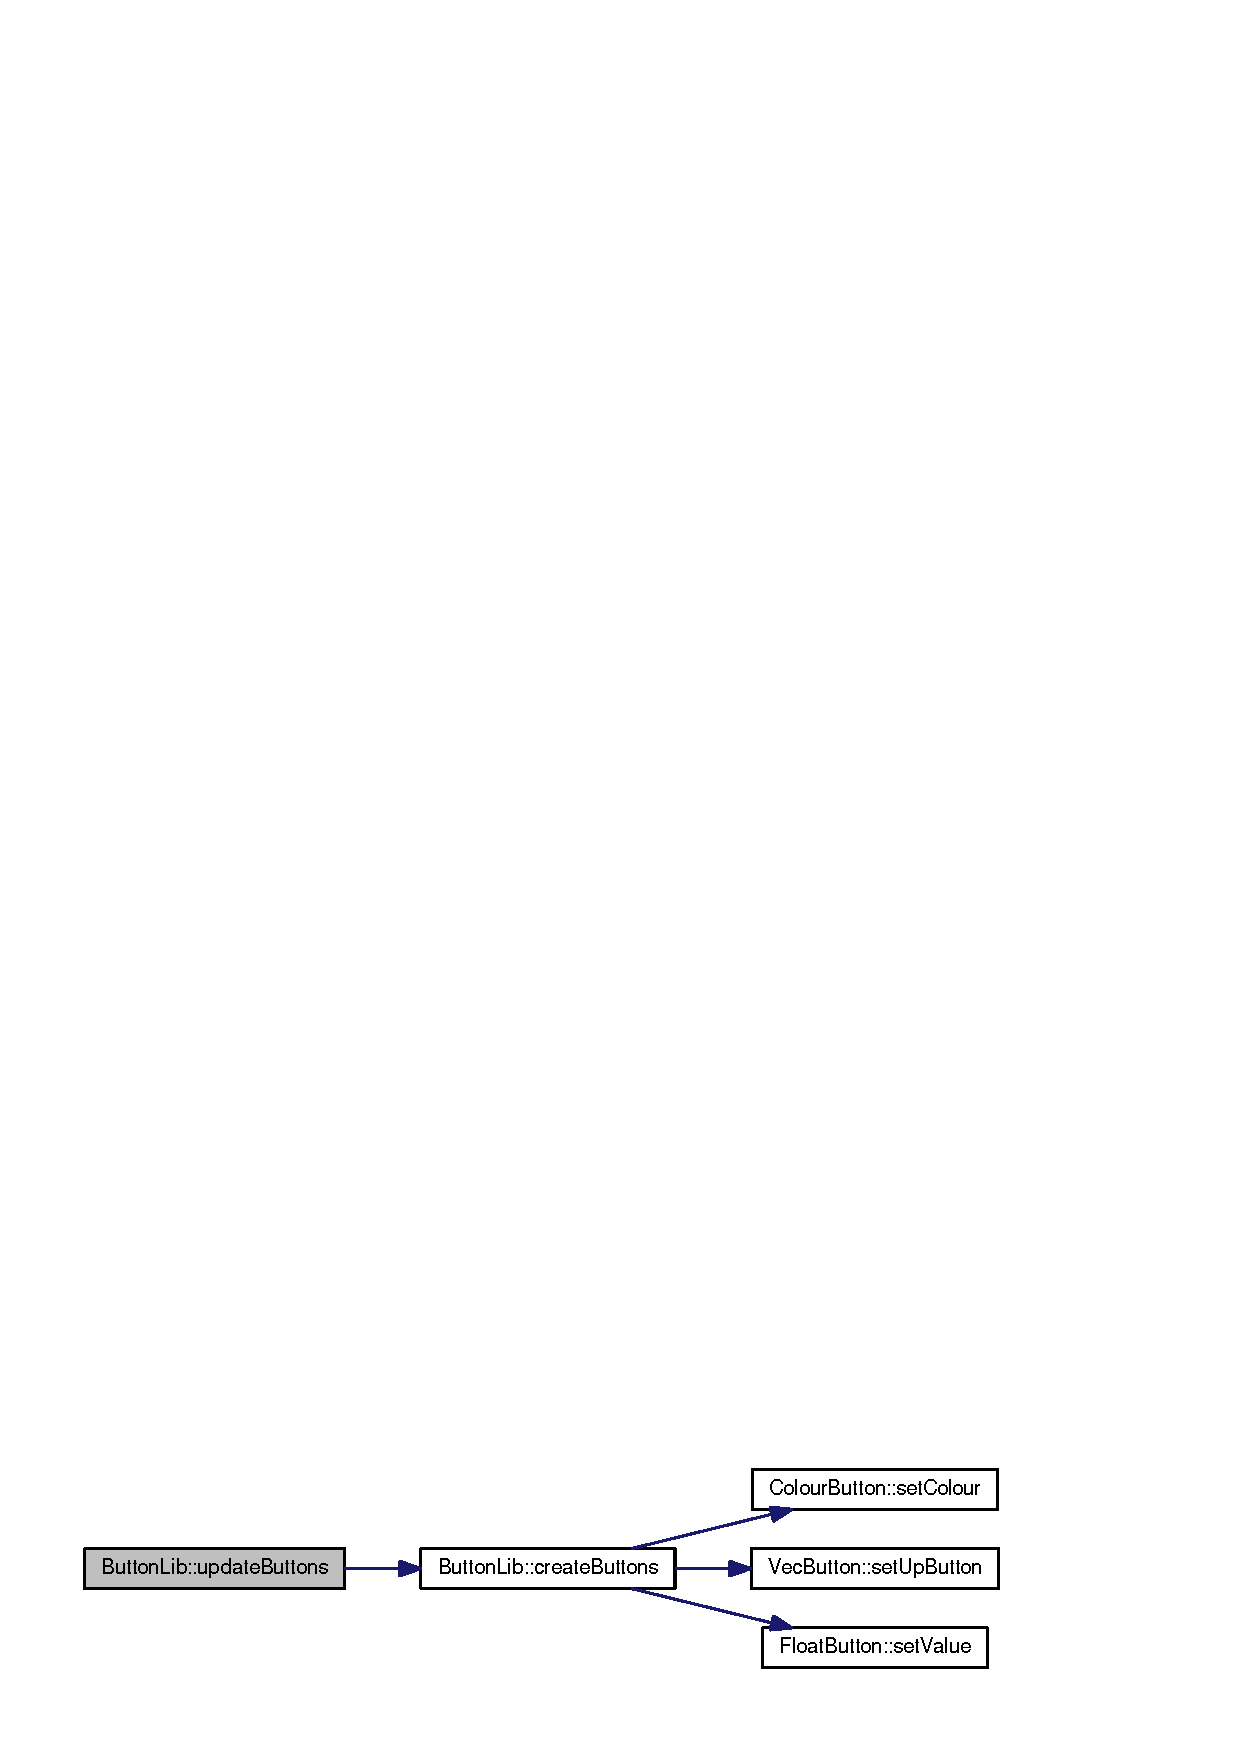
\includegraphics[width=350pt]{class_button_lib_a0b78f1baf6ff415f7f80852592fc457b_cgraph}
\end{center}
\end{figure}




Here is the caller graph for this function\-:\nopagebreak
\begin{figure}[H]
\begin{center}
\leavevmode
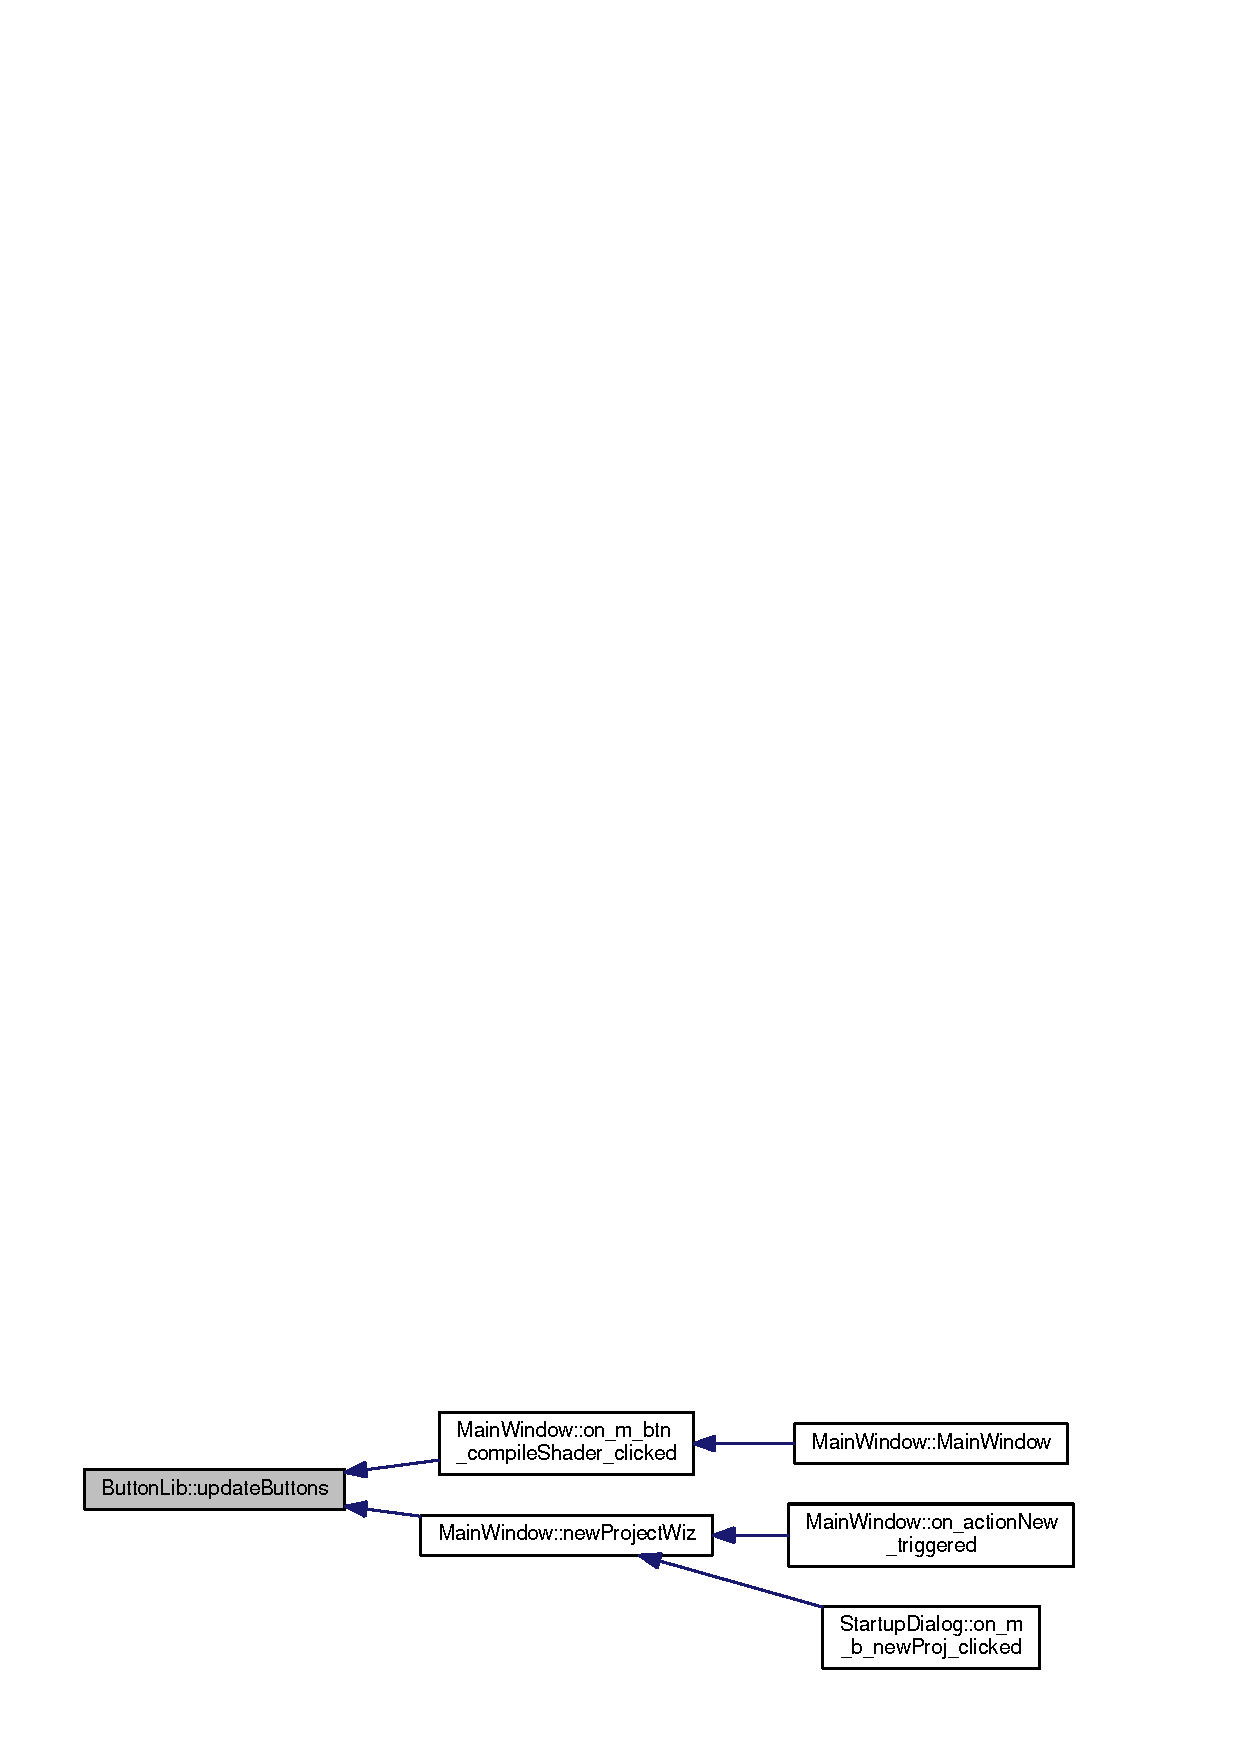
\includegraphics[width=350pt]{class_button_lib_a0b78f1baf6ff415f7f80852592fc457b_icgraph}
\end{center}
\end{figure}


\index{Button\-Lib@{Button\-Lib}!update\-Shader\-Values@{update\-Shader\-Values}}
\index{update\-Shader\-Values@{update\-Shader\-Values}!ButtonLib@{Button\-Lib}}
\subsubsection[{update\-Shader\-Values}]{\setlength{\rightskip}{0pt plus 5cm}void Button\-Lib\-::update\-Shader\-Values (
\begin{DoxyParamCaption}
{}
\end{DoxyParamCaption}
)}\label{class_button_lib_ae2644c88c1e6846a9f55b4af96dcffb9}


sets the shader values from the button values 



Definition at line 99 of file Button\-Lib.\-cpp.



References m\-\_\-button\-List, m\-\_\-parser, and Parser\-Lib\-::m\-\_\-uniform\-List.


\begin{DoxyCode}
100 \{
101   \textcolor{keywordflow}{for}(\textcolor{keyword}{auto} uniform: m_parser->m_uniformList)
102   \{
103     \textcolor{keywordflow}{if}(uniform->getTypeEnum()==GL\_FLOAT\_VEC4)
104     \{
105       \textcolor{keywordflow}{for}(\textcolor{keyword}{auto} button: m_buttonList)
106       \{
107         \textcolor{keywordflow}{if}(uniform->getLocation()==button->getID())
108         \{
109           ngl::Vec4 temp = button->getColour();
110           uniform->setVec4(temp);
111           \textcolor{keywordflow}{break};
112         \}
113       \}
114     \}
115     \textcolor{keywordflow}{if}(uniform->getTypeEnum()==GL\_FLOAT)
116     \{
117       \textcolor{keywordflow}{for}(\textcolor{keyword}{auto} button: m\_buttonList)
118       \{
119         \textcolor{keywordflow}{if}(uniform->getLocation()==button->getID())
120         \{
121           \textcolor{keywordtype}{float} temp = button->getValue();
122           uniform->setFloat(temp);
123           \textcolor{keywordflow}{break};
124         \}
125       \}
126     \}
127     \textcolor{keywordflow}{if}(uniform->getTypeEnum()==GL\_FLOAT\_VEC3)
128     \{
129       \textcolor{keywordflow}{for}(\textcolor{keyword}{auto} button: m\_buttonList)
130       \{
131         \textcolor{keywordflow}{if}(uniform->getLocation()==button->getID())
132         \{
133           ngl::Vec4 temp = button->getVec();
134           uniform->setVec3(ngl::Vec3(temp.m\_x,
135                                      temp.m\_y,
136                                      temp.m\_z));
137           ngl::Vec3 newV = uniform->getVec3();
138           \textcolor{keywordflow}{break};
139         \}
140       \}
141     \}
142   \}
143 \}
\end{DoxyCode}


Here is the caller graph for this function\-:\nopagebreak
\begin{figure}[H]
\begin{center}
\leavevmode
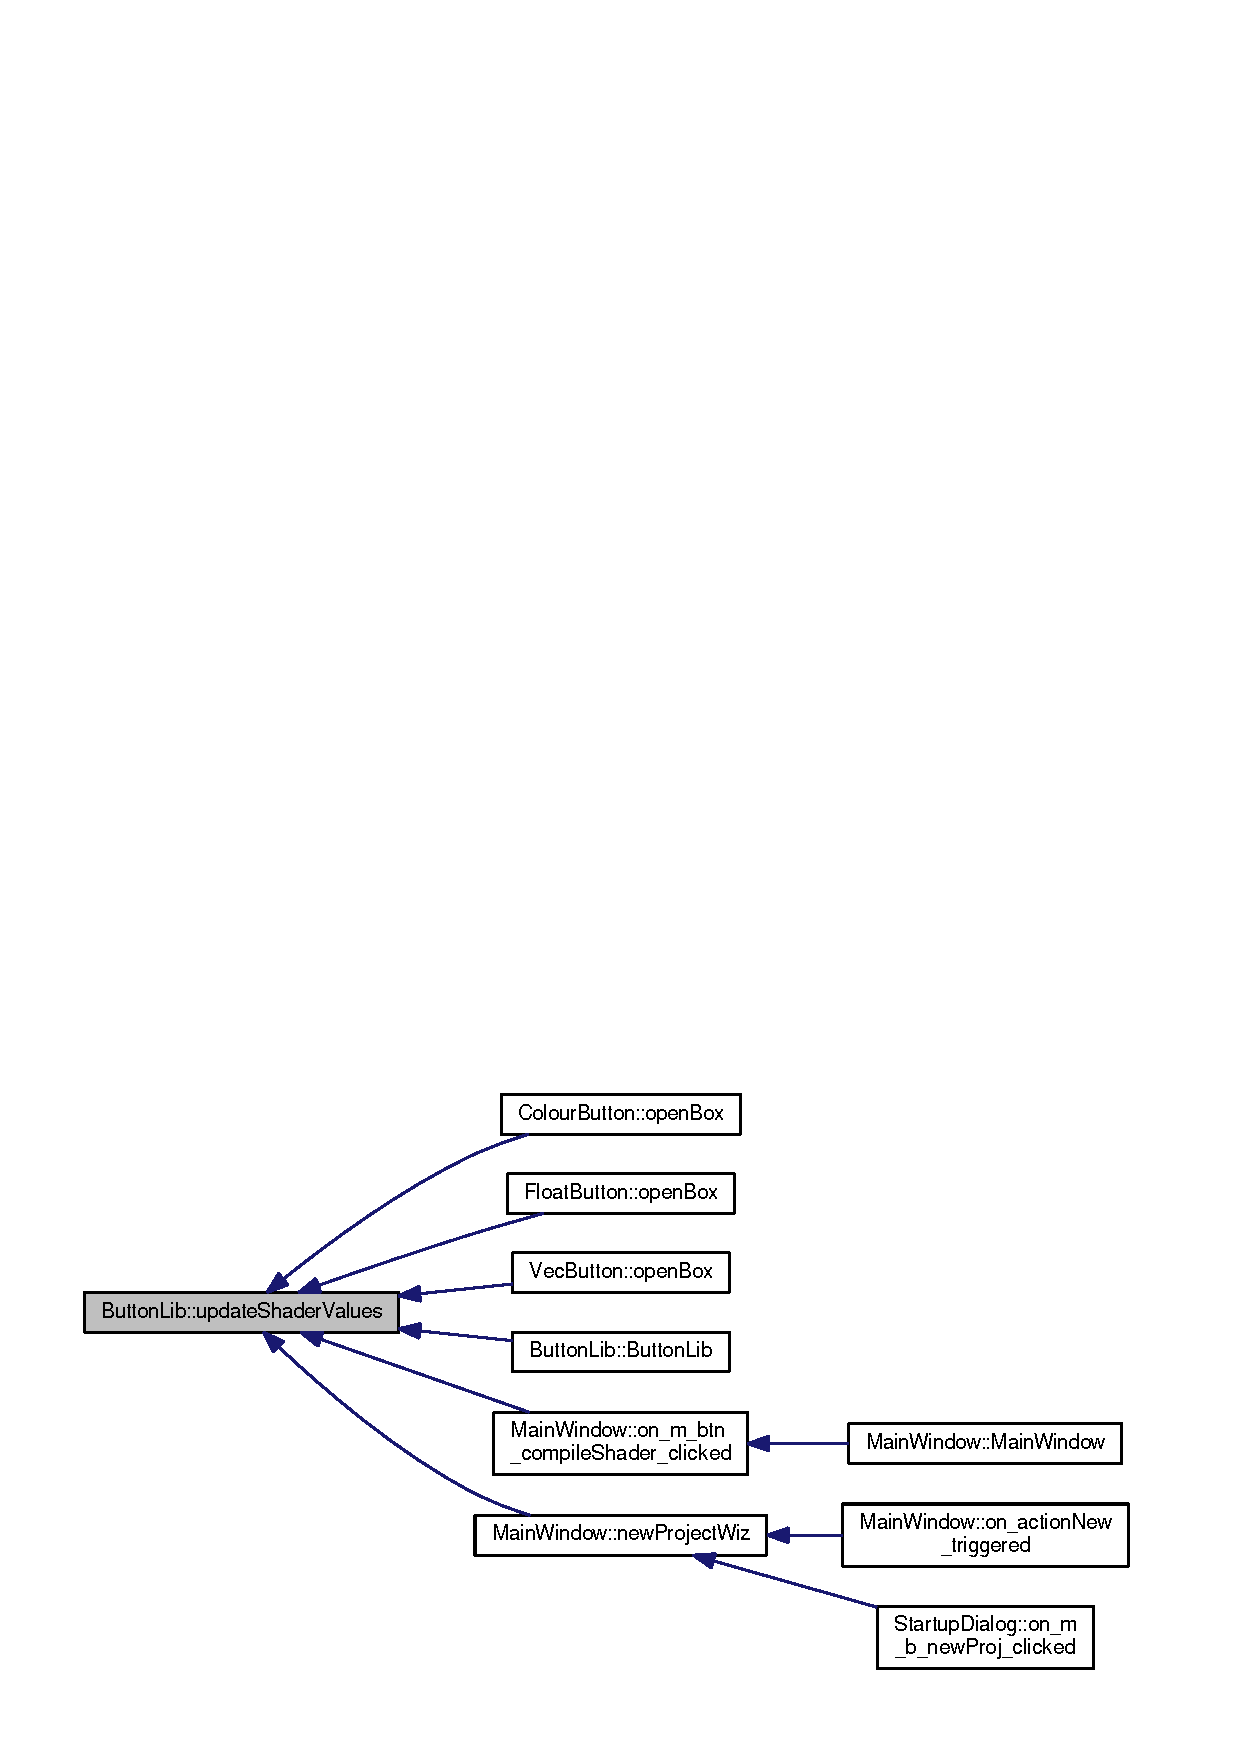
\includegraphics[width=350pt]{class_button_lib_ae2644c88c1e6846a9f55b4af96dcffb9_icgraph}
\end{center}
\end{figure}




\subsection{Member Data Documentation}
\index{Button\-Lib@{Button\-Lib}!m\-\_\-button\-List@{m\-\_\-button\-List}}
\index{m\-\_\-button\-List@{m\-\_\-button\-List}!ButtonLib@{Button\-Lib}}
\subsubsection[{m\-\_\-button\-List}]{\setlength{\rightskip}{0pt plus 5cm}std\-::vector$<${\bf Button}$\ast$$>$ Button\-Lib\-::m\-\_\-button\-List\hspace{0.3cm}{\ttfamily [private]}}\label{class_button_lib_ac5a487a895d200a4a21a3eae35b02073}


vector of buttons to dynamically and delete different types 



Definition at line 74 of file Button\-Lib.\-h.

\index{Button\-Lib@{Button\-Lib}!m\-\_\-layout@{m\-\_\-layout}}
\index{m\-\_\-layout@{m\-\_\-layout}!ButtonLib@{Button\-Lib}}
\subsubsection[{m\-\_\-layout}]{\setlength{\rightskip}{0pt plus 5cm}Q\-Layout$\ast$ Button\-Lib\-::m\-\_\-layout\hspace{0.3cm}{\ttfamily [private]}}\label{class_button_lib_ae0dc6d904c084b888aa1038e0ad0b75d}


gui layout for the buttons to be stored in 



Definition at line 58 of file Button\-Lib.\-h.

\index{Button\-Lib@{Button\-Lib}!m\-\_\-parent@{m\-\_\-parent}}
\index{m\-\_\-parent@{m\-\_\-parent}!ButtonLib@{Button\-Lib}}
\subsubsection[{m\-\_\-parent}]{\setlength{\rightskip}{0pt plus 5cm}Q\-Widget$\ast$ Button\-Lib\-::m\-\_\-parent\hspace{0.3cm}{\ttfamily [private]}}\label{class_button_lib_a8e60dd2e6cec5f9c3486882aded19f9a}


gui parent for the layout 



Definition at line 62 of file Button\-Lib.\-h.

\index{Button\-Lib@{Button\-Lib}!m\-\_\-parser@{m\-\_\-parser}}
\index{m\-\_\-parser@{m\-\_\-parser}!ButtonLib@{Button\-Lib}}
\subsubsection[{m\-\_\-parser}]{\setlength{\rightskip}{0pt plus 5cm}{\bf Parser\-Lib}$\ast$ Button\-Lib\-::m\-\_\-parser\hspace{0.3cm}{\ttfamily [private]}}\label{class_button_lib_a2d9fb2b47450133f35ce44a26930ad68}


pointer to the parser to access and set uniform values 



Definition at line 66 of file Button\-Lib.\-h.

\index{Button\-Lib@{Button\-Lib}!m\-\_\-scene@{m\-\_\-scene}}
\index{m\-\_\-scene@{m\-\_\-scene}!ButtonLib@{Button\-Lib}}
\subsubsection[{m\-\_\-scene}]{\setlength{\rightskip}{0pt plus 5cm}{\bf N\-G\-L\-Scene}$\ast$ Button\-Lib\-::m\-\_\-scene\hspace{0.3cm}{\ttfamily [private]}}\label{class_button_lib_a78b78fee74514bc97bbf8f5a6e19fe64}


pointer to the \doxyref{N\-G\-L\-Scene}{p.}{class_n_g_l_scene}, gl Widget 



Definition at line 70 of file Button\-Lib.\-h.



The documentation for this class was generated from the following files\-:\begin{DoxyCompactItemize}
\item 
{\bf Button\-Lib.\-h}\item 
{\bf Button\-Lib.\-cpp}\end{DoxyCompactItemize}

\section{Camera Class Reference}
\label{class_camera}\index{Camera@{Camera}}


Manages using multiple cameras in \doxyref{N\-G\-L\-Scene}{p.}{class_n_g_l_scene}.  




{\ttfamily \#include $<$Camera.\-h$>$}



Inheritance diagram for Camera\-:\nopagebreak
\begin{figure}[H]
\begin{center}
\leavevmode
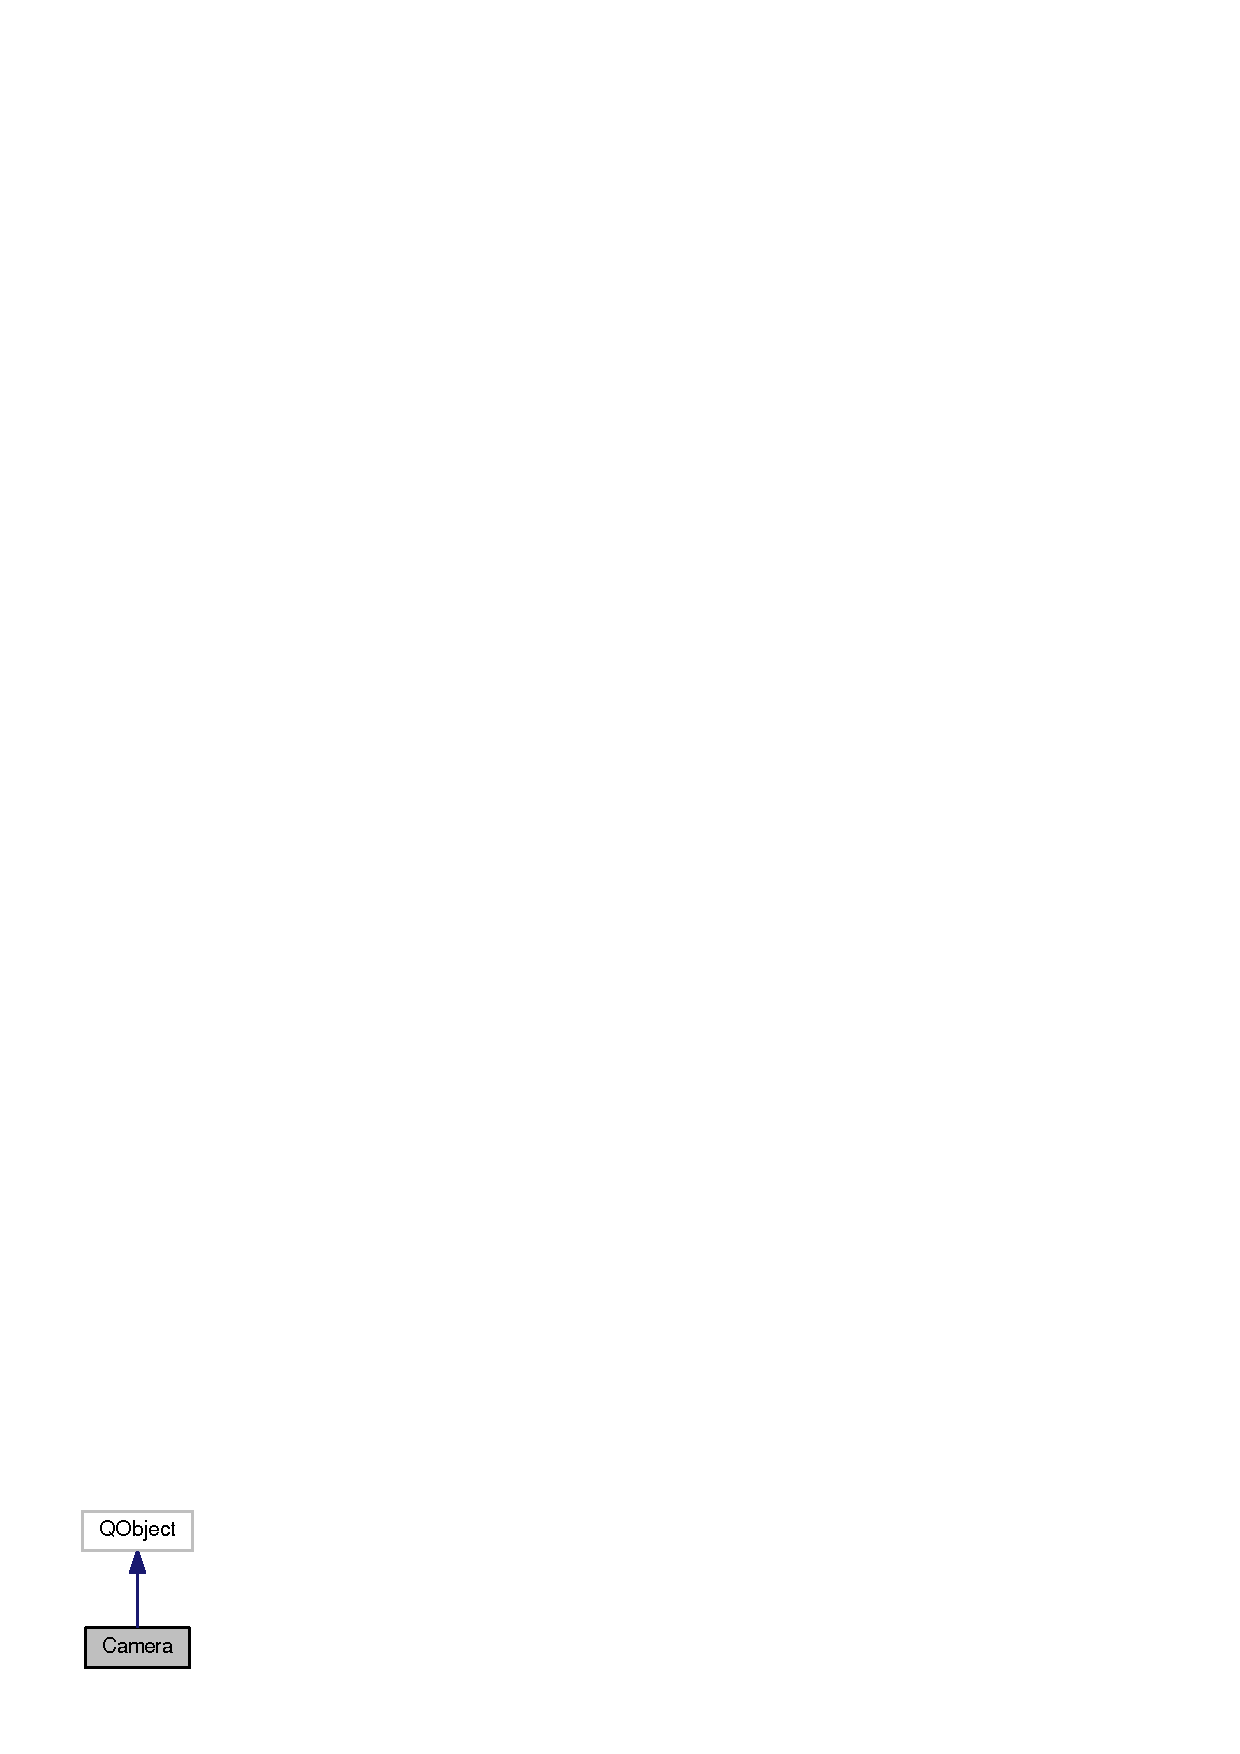
\includegraphics[width=96pt]{class_camera__inherit__graph}
\end{center}
\end{figure}


Collaboration diagram for Camera\-:\nopagebreak
\begin{figure}[H]
\begin{center}
\leavevmode
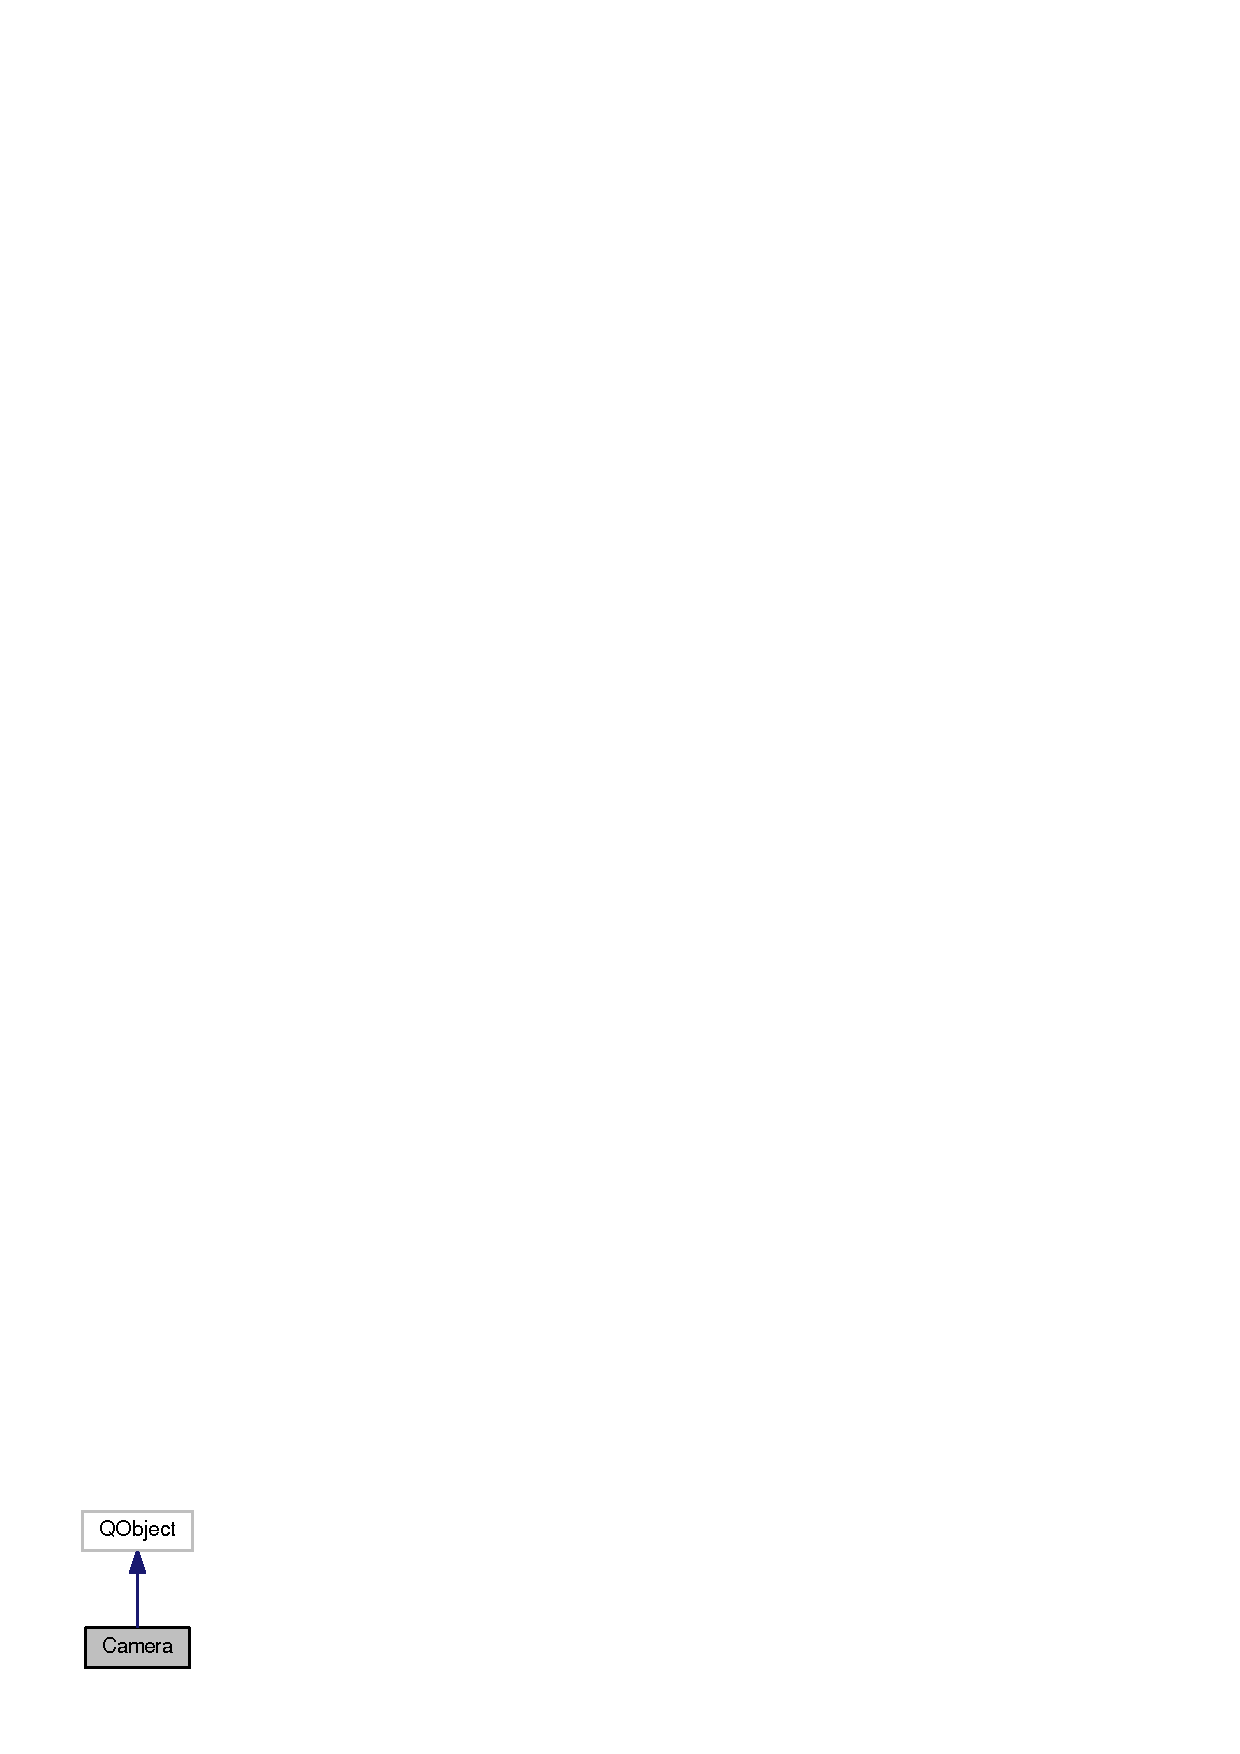
\includegraphics[width=96pt]{class_camera__coll__graph}
\end{center}
\end{figure}
\subsection*{Public Slots}
\begin{DoxyCompactItemize}
\item 
void {\bf set\-Camera\-Focal\-Length} (int \-\_\-focal\-Length)
\begin{DoxyCompactList}\small\item\em Function to set camera F\-O\-V. \end{DoxyCompactList}\item 
void {\bf set\-Camera\-Shape} (Q\-String \-\_\-view)
\begin{DoxyCompactList}\small\item\em Sets the new camera shape. \end{DoxyCompactList}\item 
void {\bf camera\-Roll} (double \-\_\-camera\-Roll)
\begin{DoxyCompactList}\small\item\em Sets camera roll. \end{DoxyCompactList}\item 
void {\bf camera\-Pitch} (double \-\_\-camera\-Pitch)
\begin{DoxyCompactList}\small\item\em Sets camera Pitch. \end{DoxyCompactList}\item 
void {\bf camera\-Yaw} (double \-\_\-camera\-Yaw)
\begin{DoxyCompactList}\small\item\em Sets camera Yaw. \end{DoxyCompactList}\item 
void {\bf set\-Cam\-Near\-Clip} (double \-\_\-near\-Clip)
\begin{DoxyCompactList}\small\item\em Sets near clipping frame. \end{DoxyCompactList}\item 
void {\bf set\-Cam\-Far\-Clip} (double \-\_\-far\-Clip)
\begin{DoxyCompactList}\small\item\em Sets far clipping frame. \end{DoxyCompactList}\end{DoxyCompactItemize}
\subsection*{Signals}
\begin{DoxyCompactItemize}
\item 
void {\bf update\-Signal} ()
\begin{DoxyCompactList}\small\item\em Signal sent to \doxyref{N\-G\-L\-Scene}{p.}{class_n_g_l_scene} update() function to update the scene with the new camera. \end{DoxyCompactList}\end{DoxyCompactItemize}
\subsection*{Public Member Functions}
\begin{DoxyCompactItemize}
\item 
{\bf Camera} ()
\begin{DoxyCompactList}\small\item\em \-\_\-\-Cstor class \end{DoxyCompactList}\item 
void {\bf create\-Cameras} ()
\begin{DoxyCompactList}\small\item\em Creates a vector of ngl cameras and sets their shapes. \end{DoxyCompactList}\item 
ngl\-::\-Camera {\bf set\-Shape\-Cam} ()
\begin{DoxyCompactList}\small\item\em Sets the camera shape and returns the new camera to \doxyref{N\-G\-L\-Scene}{p.}{class_n_g_l_scene}. \end{DoxyCompactList}\end{DoxyCompactItemize}
\subsection*{Public Attributes}
\begin{DoxyCompactItemize}
\item 
std\-::vector$<$ ngl\-::\-Camera $>$ {\bf m\-\_\-cameras}
\begin{DoxyCompactList}\small\item\em A vector containing the ngl cameras. \end{DoxyCompactList}\item 
int {\bf m\-\_\-camera\-Index}
\begin{DoxyCompactList}\small\item\em An index to access the cameras. \end{DoxyCompactList}\item 
int {\bf m\-\_\-fov}
\begin{DoxyCompactList}\small\item\em fov value for the camera \end{DoxyCompactList}\item 
float {\bf m\-\_\-aspect}
\begin{DoxyCompactList}\small\item\em aspect ratio of the camera \end{DoxyCompactList}\item 
float {\bf m\-\_\-near\-Clip}
\begin{DoxyCompactList}\small\item\em Near clipping plane of the camera. \end{DoxyCompactList}\item 
float {\bf m\-\_\-far\-Clip}
\begin{DoxyCompactList}\small\item\em Far clipping plane of the camera. \end{DoxyCompactList}\item 
double {\bf m\-\_\-camera\-Yaw}
\begin{DoxyCompactList}\small\item\em camera yaw value \end{DoxyCompactList}\item 
double {\bf m\-\_\-camera\-Roll}
\begin{DoxyCompactList}\small\item\em camera roll value \end{DoxyCompactList}\item 
double {\bf m\-\_\-camera\-Pitch}
\begin{DoxyCompactList}\small\item\em camera pitch value \end{DoxyCompactList}\item 
ngl\-::\-Camera {\bf m\-\_\-main\-Camera}
\begin{DoxyCompactList}\small\item\em Active camera used by \doxyref{N\-G\-L\-Scene}{p.}{class_n_g_l_scene}. \end{DoxyCompactList}\end{DoxyCompactItemize}


\subsection{Detailed Description}
Manages using multiple cameras in \doxyref{N\-G\-L\-Scene}{p.}{class_n_g_l_scene}. 

Definition at line 26 of file Camera.\-h.



\subsection{Constructor \& Destructor Documentation}
\index{Camera@{Camera}!Camera@{Camera}}
\index{Camera@{Camera}!Camera@{Camera}}
\subsubsection[{Camera}]{\setlength{\rightskip}{0pt plus 5cm}Camera\-::\-Camera (
\begin{DoxyParamCaption}
{}
\end{DoxyParamCaption}
)}\label{class_camera_a01f94c3543f56ede7af49dc778f19331}


\-\_\-\-Cstor class 



Definition at line 5 of file Camera.\-cpp.



References m\-\_\-camera\-Index, m\-\_\-camera\-Roll, m\-\_\-camera\-Yaw, m\-\_\-far\-Clip, m\-\_\-fov, and m\-\_\-near\-Clip.


\begin{DoxyCode}
6 \{
7     m_fov=60.0;
8     m_cameraIndex = 0;
9     m_cameraRoll = 0.00;
10     m_cameraYaw = 0.00;
11     m_nearClip = 0.5f;
12     m_farClip = 150.0f;
13 \}
\end{DoxyCode}


\subsection{Member Function Documentation}
\index{Camera@{Camera}!camera\-Pitch@{camera\-Pitch}}
\index{camera\-Pitch@{camera\-Pitch}!Camera@{Camera}}
\subsubsection[{camera\-Pitch}]{\setlength{\rightskip}{0pt plus 5cm}void Camera\-::camera\-Pitch (
\begin{DoxyParamCaption}
\item[{double}]{\-\_\-camera\-Pitch}
\end{DoxyParamCaption}
)\hspace{0.3cm}{\ttfamily [slot]}}\label{class_camera_a0c0d93f08f72642a944eb7514d81c0d8}


Sets camera Pitch. 


\begin{DoxyParams}[1]{Parameters}
\mbox{\tt in}  & {\em \-\_\-camera\-Pitch} & the new pitch value \\
\hline
\end{DoxyParams}


Definition at line 93 of file Camera.\-cpp.



References m\-\_\-camera\-Pitch, m\-\_\-main\-Camera, and update\-Signal().


\begin{DoxyCode}
94 \{
95     m_mainCamera.pitch(-m_cameraPitch);
96     m_cameraPitch = \_cameraPitch;
97     m_mainCamera.pitch(\_cameraPitch);
98     emit updateSignal();
99 \}
\end{DoxyCode}


Here is the caller graph for this function\-:\nopagebreak
\begin{figure}[H]
\begin{center}
\leavevmode
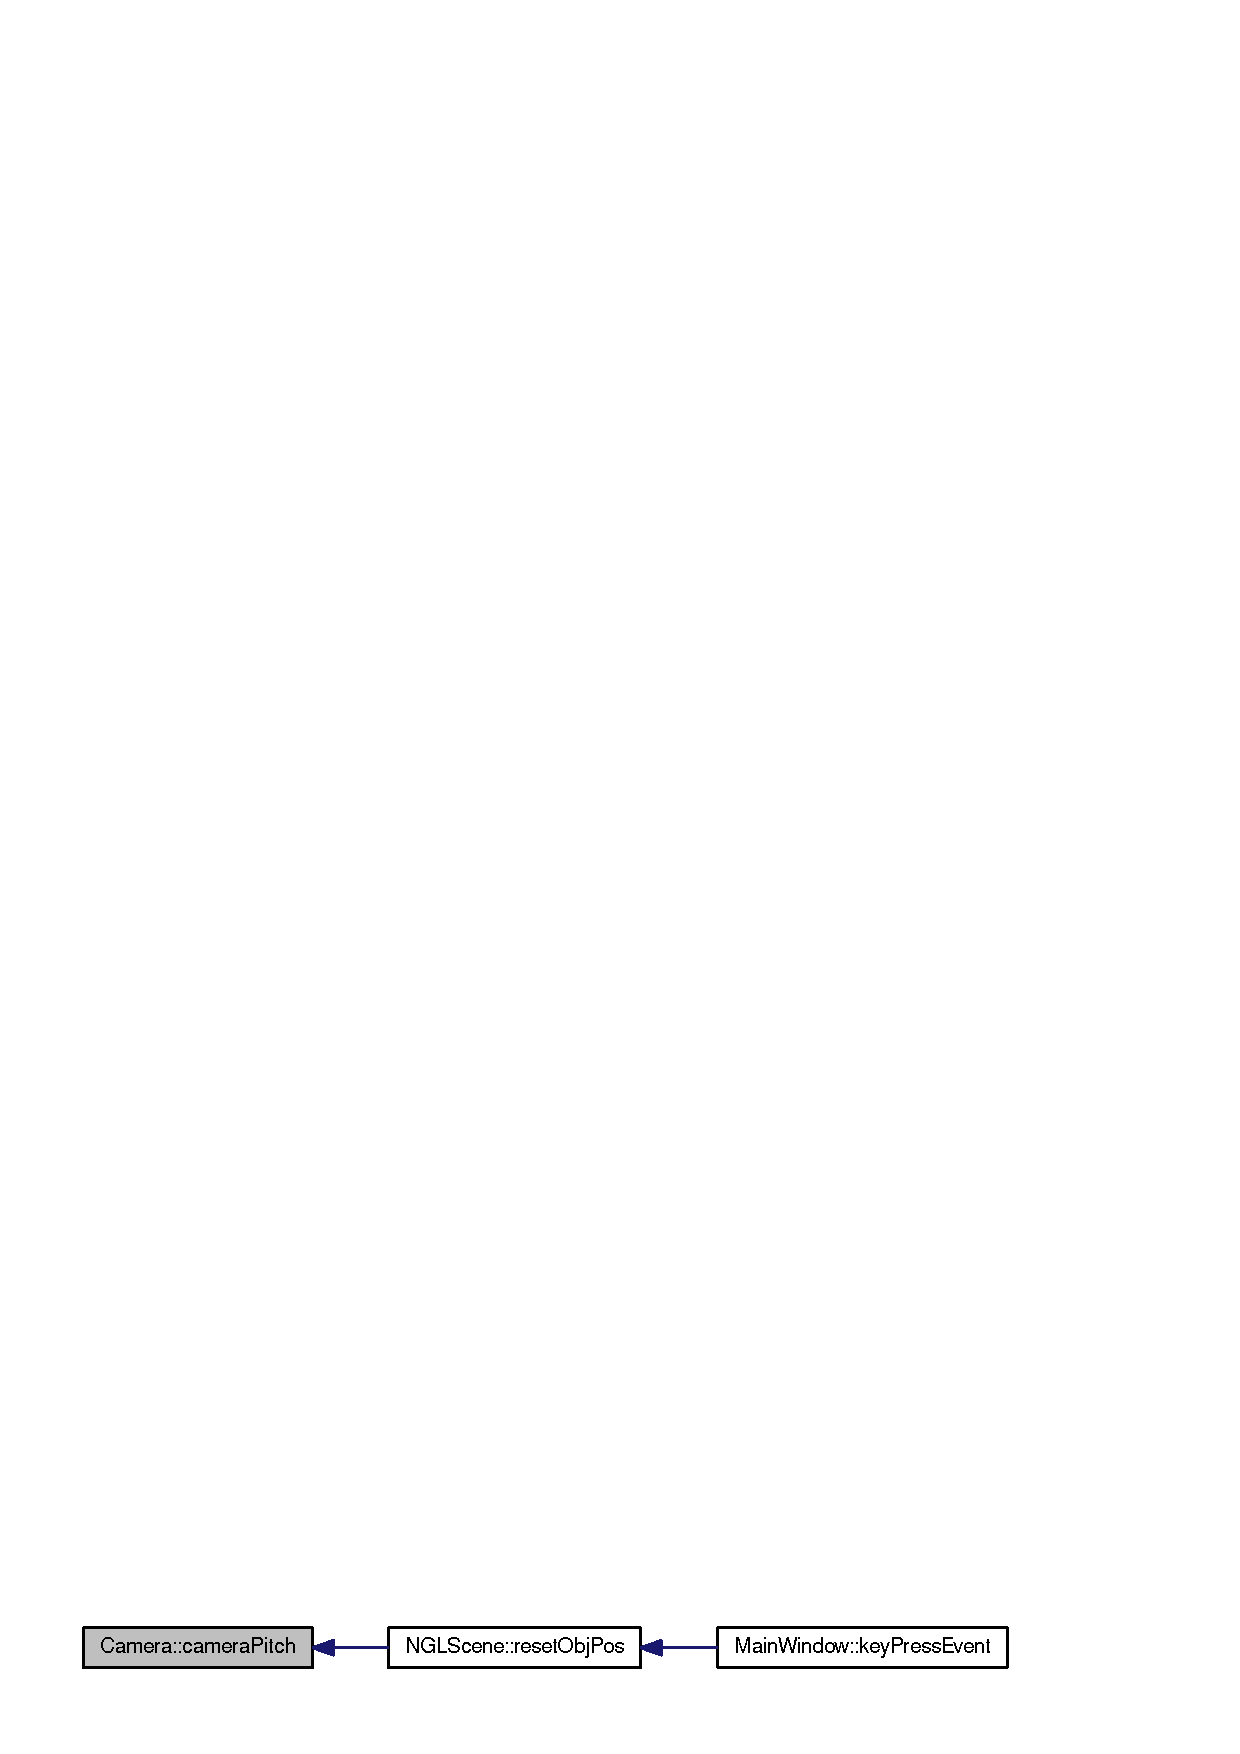
\includegraphics[width=350pt]{class_camera_a0c0d93f08f72642a944eb7514d81c0d8_icgraph}
\end{center}
\end{figure}


\index{Camera@{Camera}!camera\-Roll@{camera\-Roll}}
\index{camera\-Roll@{camera\-Roll}!Camera@{Camera}}
\subsubsection[{camera\-Roll}]{\setlength{\rightskip}{0pt plus 5cm}void Camera\-::camera\-Roll (
\begin{DoxyParamCaption}
\item[{double}]{\-\_\-camera\-Roll}
\end{DoxyParamCaption}
)\hspace{0.3cm}{\ttfamily [slot]}}\label{class_camera_ab78d1a3c0f1d2260fcf962cc5589f8b4}


Sets camera roll. 


\begin{DoxyParams}[1]{Parameters}
\mbox{\tt in}  & {\em \-\_\-camera\-Roll} & the new roll value \\
\hline
\end{DoxyParams}


Definition at line 104 of file Camera.\-cpp.



References m\-\_\-camera\-Roll, m\-\_\-main\-Camera, and update\-Signal().


\begin{DoxyCode}
105 \{
106     m_mainCamera.roll(-m_cameraRoll);
107     m_cameraRoll = \_cameraRoll;
108     m_mainCamera.roll(\_cameraRoll);
109     emit updateSignal();
110 \}
\end{DoxyCode}


Here is the caller graph for this function\-:\nopagebreak
\begin{figure}[H]
\begin{center}
\leavevmode
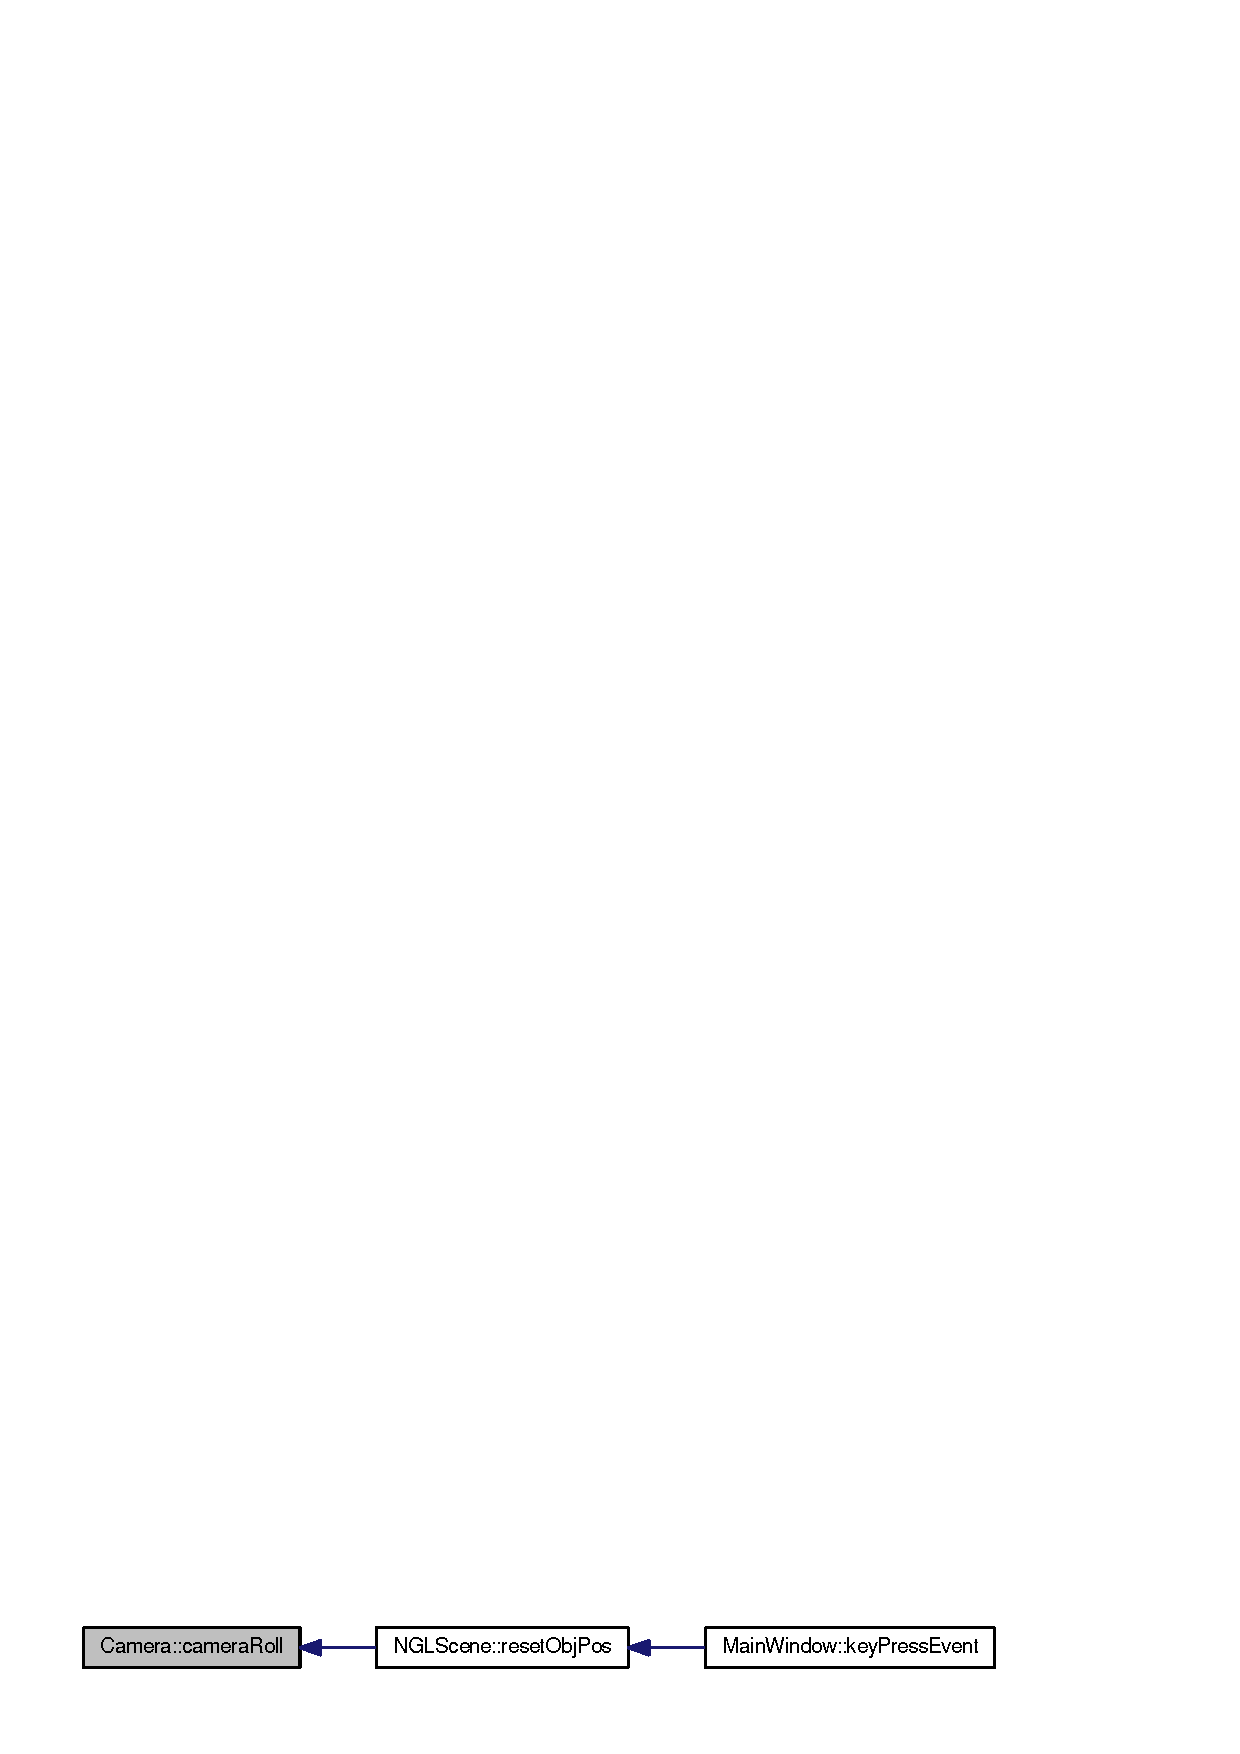
\includegraphics[width=350pt]{class_camera_ab78d1a3c0f1d2260fcf962cc5589f8b4_icgraph}
\end{center}
\end{figure}


\index{Camera@{Camera}!camera\-Yaw@{camera\-Yaw}}
\index{camera\-Yaw@{camera\-Yaw}!Camera@{Camera}}
\subsubsection[{camera\-Yaw}]{\setlength{\rightskip}{0pt plus 5cm}void Camera\-::camera\-Yaw (
\begin{DoxyParamCaption}
\item[{double}]{\-\_\-camera\-Yaw}
\end{DoxyParamCaption}
)\hspace{0.3cm}{\ttfamily [slot]}}\label{class_camera_a5f14cfea1ff576e947bddae2139ca078}


Sets camera Yaw. 


\begin{DoxyParams}[1]{Parameters}
\mbox{\tt in}  & {\em \-\_\-camera\-Yaw} & the new yaw value \\
\hline
\end{DoxyParams}


Definition at line 82 of file Camera.\-cpp.



References m\-\_\-camera\-Yaw, m\-\_\-main\-Camera, and update\-Signal().


\begin{DoxyCode}
83 \{
84     m_mainCamera.yaw(-m_cameraYaw);
85     m_cameraYaw = \_cameraYaw;
86     m_mainCamera.yaw(\_cameraYaw);
87     emit updateSignal();
88 \}
\end{DoxyCode}


Here is the caller graph for this function\-:\nopagebreak
\begin{figure}[H]
\begin{center}
\leavevmode
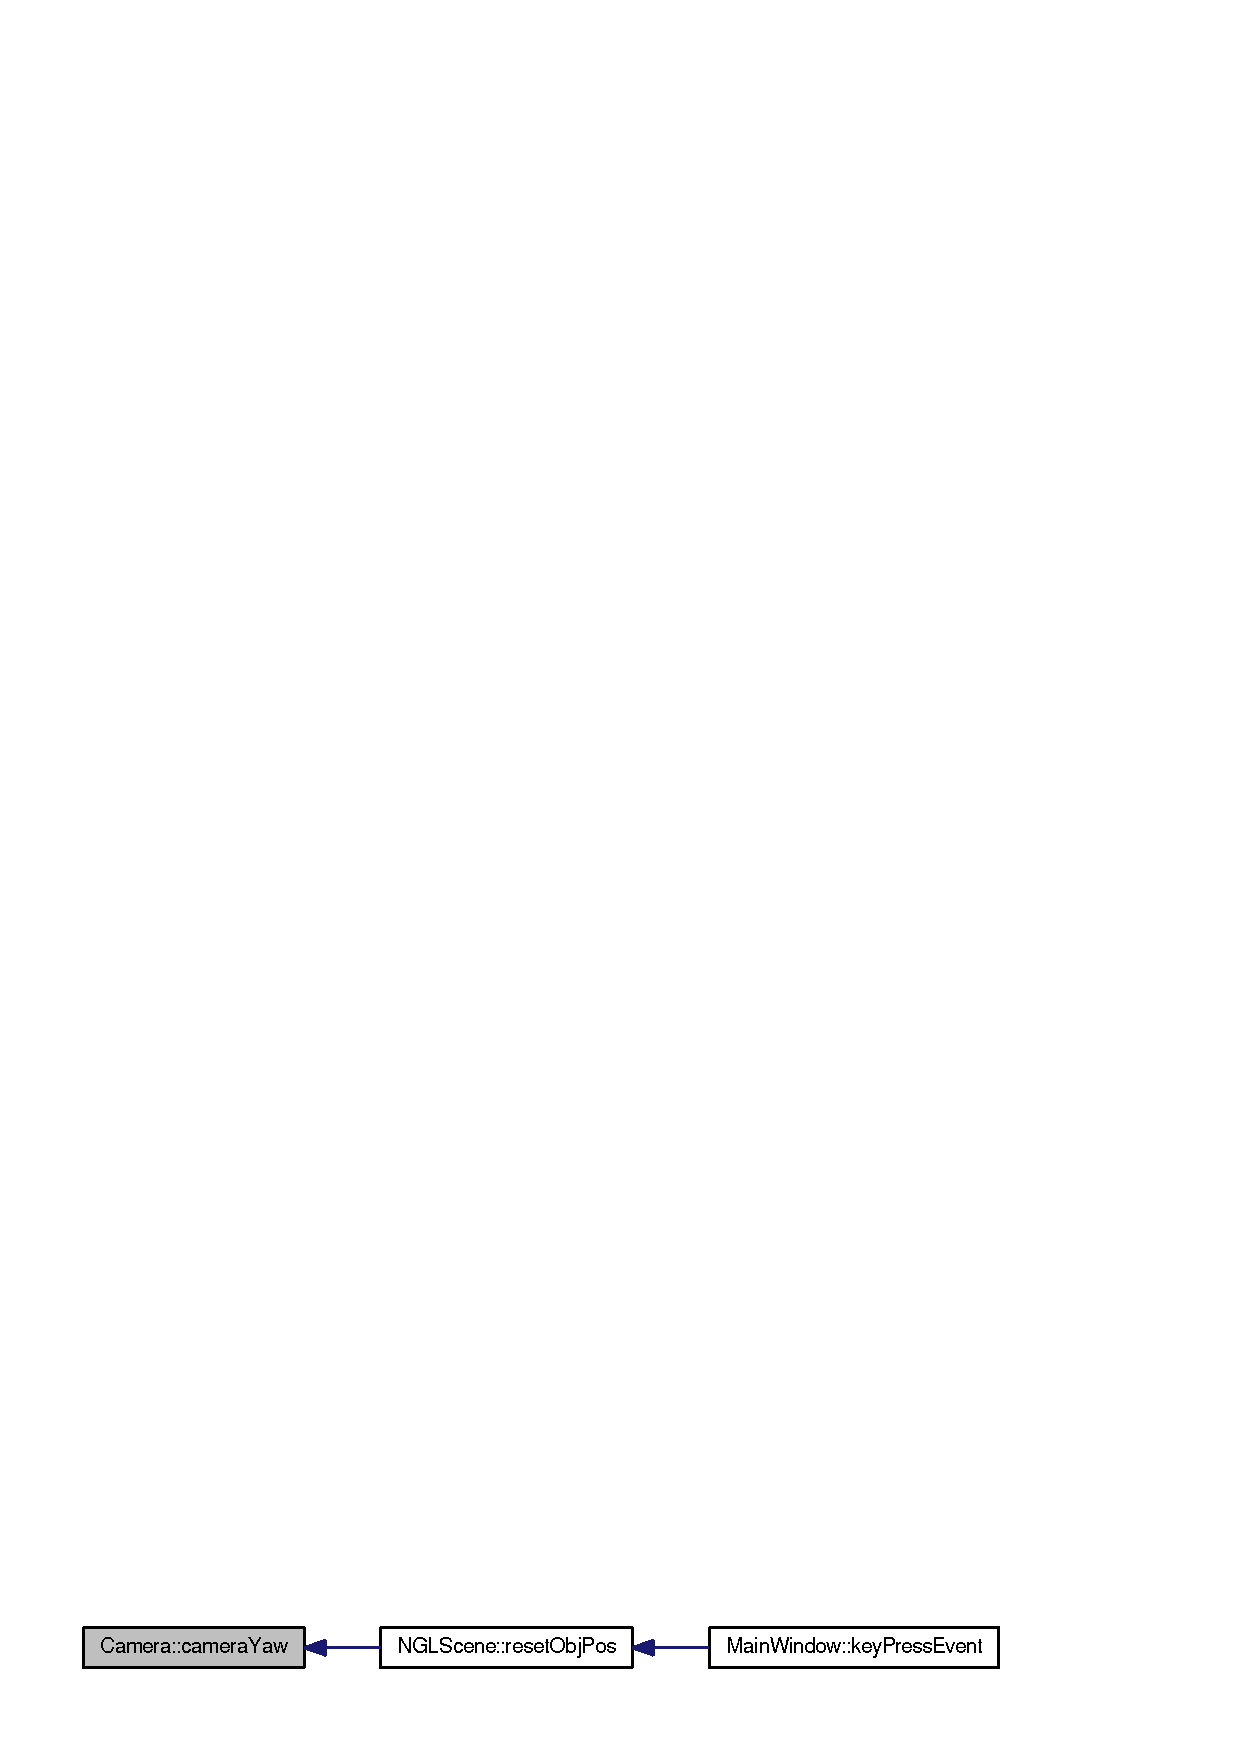
\includegraphics[width=350pt]{class_camera_a5f14cfea1ff576e947bddae2139ca078_icgraph}
\end{center}
\end{figure}


\index{Camera@{Camera}!create\-Cameras@{create\-Cameras}}
\index{create\-Cameras@{create\-Cameras}!Camera@{Camera}}
\subsubsection[{create\-Cameras}]{\setlength{\rightskip}{0pt plus 5cm}void Camera\-::create\-Cameras (
\begin{DoxyParamCaption}
{}
\end{DoxyParamCaption}
)}\label{class_camera_a0b2c173335886d0f85085dae91e7305c}


Creates a vector of ngl cameras and sets their shapes. 



Definition at line 17 of file Camera.\-cpp.



References m\-\_\-aspect, m\-\_\-camera\-Index, m\-\_\-cameras, m\-\_\-fov, and m\-\_\-main\-Camera.


\begin{DoxyCode}
18 \{
19     \textcolor{comment}{// Initialises ngl cameras.}
20     ngl::Camera Pcam;
21     ngl::Camera Tcam;
22     ngl::Camera Bcam;
23     ngl::Camera Lcam;
24     ngl::Camera Rcam;
25 
26     \textcolor{comment}{// Sets the eye, look, up position vectors of the cameras.}
27     ngl::Vec3 perspEye(-1.0f, 1.0f,1.0f);
28     ngl::Vec3 perspLook(0,0,0);
29     ngl::Vec3 perspUp(0.0f,1.0f,0.0f);
30 
31     ngl::Vec3 topEye(0.0f,1.0f,0.0f);
32     ngl::Vec3 topLook(0,0,0);
33     ngl::Vec3 topUp(0.0f,0.0f,1.0f);
34 
35     ngl::Vec3 bottomEye(0.0f,-1.0f,0.0f);
36     ngl::Vec3 bottomLook(0,0,0);
37     ngl::Vec3 bottomUp(0.0f,0.0f,1.0f);
38 
39     ngl::Vec3 leftEye(0.0f,0.0f,-1.0f);
40     ngl::Vec3 leftLook(0,0,0);
41     ngl::Vec3 leftUp(0.0f,1.0f,0.0f);
42 
43     ngl::Vec3 rightEye(0.0f,0.0f,1.0f);
44     ngl::Vec3 rightLook(0,0,0);
45     ngl::Vec3 rightUp(0.0f,1.0f,0.0f);
46 
47     \textcolor{comment}{// Applies the camera positions and sets their shapes, then pushes to the vector of cameras.}
48     Pcam.set(perspEye,perspLook, perspUp);
49     Pcam.setShape(m_fov,m_aspect, 0.5f,150.0f);
50     m_cameras.push\_back(Pcam);
51 
52     Tcam.set(topEye,topLook,topUp);
53     Tcam.setShape(m_fov,m_aspect, 0.5f,150.0f);
54     m_cameras.push\_back(Tcam);
55 
56     Bcam.set(bottomEye,bottomLook,bottomUp);
57     Bcam.setShape(m_fov,m_aspect, 0.5f,150.0f);
58     m_cameras.push\_back(Bcam);
59 
60     Lcam.set(leftEye,leftLook,leftUp);
61     Lcam.setShape(m_fov,m_aspect, 0.5f,150.0f);
62     m_cameras.push\_back(Lcam);
63 
64     Rcam.set(rightEye,rightLook,rightUp);
65     Rcam.setShape(m_fov,m_aspect, 0.5f,150.0f);
66     m_cameras.push\_back(Rcam);
67 
68     \textcolor{comment}{// Active camera used by NGLScene.}
69     m_mainCamera = m_cameras[m_cameraIndex];
70 \}
\end{DoxyCode}


Here is the caller graph for this function\-:\nopagebreak
\begin{figure}[H]
\begin{center}
\leavevmode
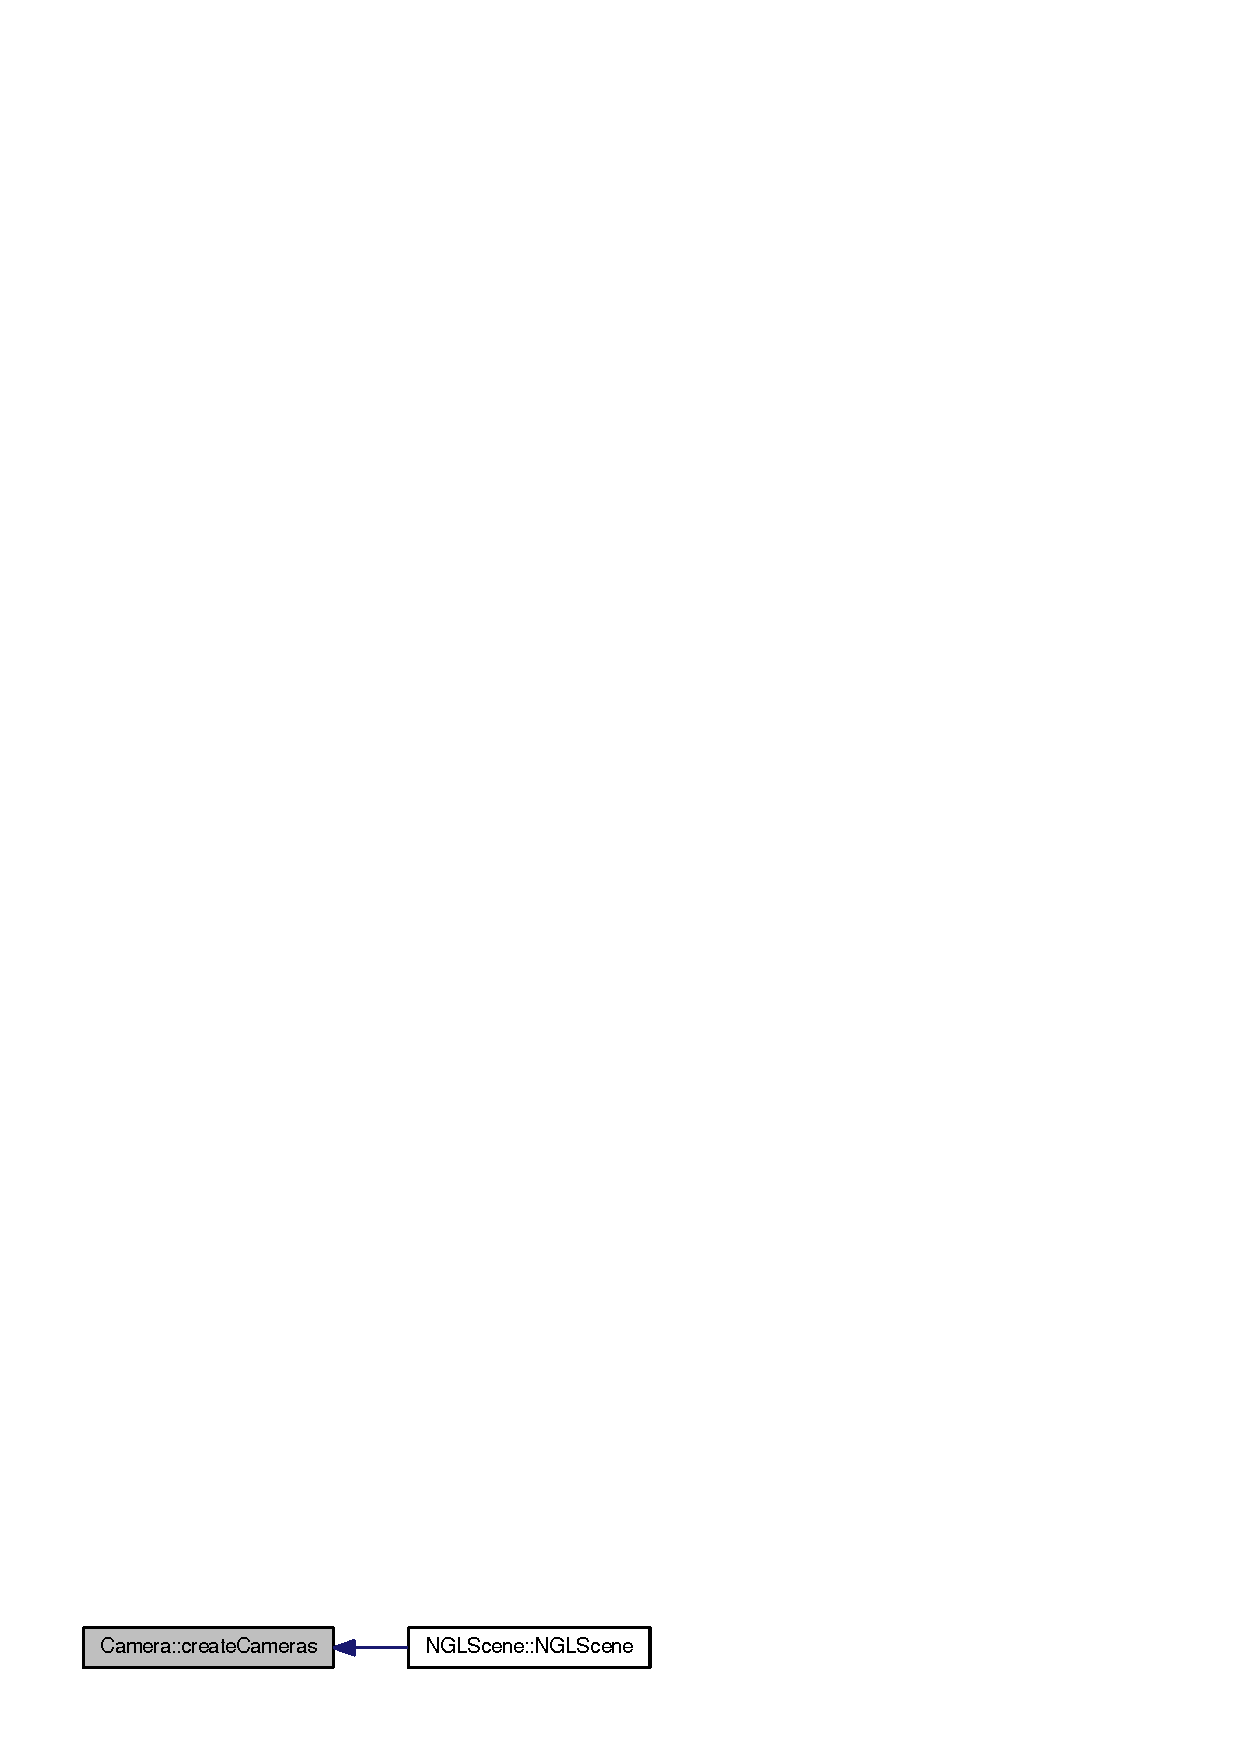
\includegraphics[width=316pt]{class_camera_a0b2c173335886d0f85085dae91e7305c_icgraph}
\end{center}
\end{figure}


\index{Camera@{Camera}!set\-Camera\-Focal\-Length@{set\-Camera\-Focal\-Length}}
\index{set\-Camera\-Focal\-Length@{set\-Camera\-Focal\-Length}!Camera@{Camera}}
\subsubsection[{set\-Camera\-Focal\-Length}]{\setlength{\rightskip}{0pt plus 5cm}void Camera\-::set\-Camera\-Focal\-Length (
\begin{DoxyParamCaption}
\item[{int}]{\-\_\-focal\-Length}
\end{DoxyParamCaption}
)\hspace{0.3cm}{\ttfamily [slot]}}\label{class_camera_aa4296a894d5a5b2dd4031efbed9d83f8}


Function to set camera F\-O\-V. 


\begin{DoxyParams}[1]{Parameters}
\mbox{\tt in}  & {\em \-\_\-focal\-Length} & the F\-O\-V value to set \\
\hline
\end{DoxyParams}


Definition at line 114 of file Camera.\-cpp.



References m\-\_\-aspect, m\-\_\-fov, m\-\_\-main\-Camera, and update\-Signal().


\begin{DoxyCode}
115 \{
116     m_fov= \_focalLength;
117     m_mainCamera.setShape(m_fov, m_aspect, 0.5f, 150.0f);
118     emit updateSignal();
119 \}
\end{DoxyCode}
\index{Camera@{Camera}!set\-Camera\-Shape@{set\-Camera\-Shape}}
\index{set\-Camera\-Shape@{set\-Camera\-Shape}!Camera@{Camera}}
\subsubsection[{set\-Camera\-Shape}]{\setlength{\rightskip}{0pt plus 5cm}void Camera\-::set\-Camera\-Shape (
\begin{DoxyParamCaption}
\item[{Q\-String}]{\-\_\-view}
\end{DoxyParamCaption}
)\hspace{0.3cm}{\ttfamily [slot]}}\label{class_camera_a3a809a3fa14f21bfd71867a680311192}


Sets the new camera shape. 


\begin{DoxyParams}[1]{Parameters}
\mbox{\tt in}  & {\em \-\_\-view} & The camera view set (persp, top, bottom, left, right). \\
\hline
\end{DoxyParams}


Definition at line 124 of file Camera.\-cpp.



References m\-\_\-camera\-Index, m\-\_\-cameras, m\-\_\-main\-Camera, and update\-Signal().


\begin{DoxyCode}
125 \{
126   std::string view = \_view.toStdString();
127 
128   std::map<std::string, int> camViewMap;
129   camViewMap[\textcolor{stringliteral}{"Persp"}]=0;
130   camViewMap[\textcolor{stringliteral}{"Top"}]=1;
131   camViewMap[\textcolor{stringliteral}{"Bottom"}]=2;
132   camViewMap[\textcolor{stringliteral}{"Left"}]=3;
133   camViewMap[\textcolor{stringliteral}{"Right"}]=4;
134 
135   m_cameraIndex = camViewMap[view];
136   m_mainCamera = m_cameras[m_cameraIndex];
137 
138   emit updateSignal();
139 \}
\end{DoxyCode}
\index{Camera@{Camera}!set\-Cam\-Far\-Clip@{set\-Cam\-Far\-Clip}}
\index{set\-Cam\-Far\-Clip@{set\-Cam\-Far\-Clip}!Camera@{Camera}}
\subsubsection[{set\-Cam\-Far\-Clip}]{\setlength{\rightskip}{0pt plus 5cm}void Camera\-::set\-Cam\-Far\-Clip (
\begin{DoxyParamCaption}
\item[{double}]{\-\_\-far\-Clip}
\end{DoxyParamCaption}
)\hspace{0.3cm}{\ttfamily [slot]}}\label{class_camera_a6ebda712bd672e403b2fea35f46425c2}


Sets far clipping frame. 


\begin{DoxyParams}[1]{Parameters}
\mbox{\tt in}  & {\em \-\_\-far\-Clip} & the far clipping plane value \\
\hline
\end{DoxyParams}


Definition at line 152 of file Camera.\-cpp.



References m\-\_\-far\-Clip, and update\-Signal().


\begin{DoxyCode}
153 \{
154     m_farClip= \_farClip;
155     emit updateSignal();
156 \}
\end{DoxyCode}
\index{Camera@{Camera}!set\-Cam\-Near\-Clip@{set\-Cam\-Near\-Clip}}
\index{set\-Cam\-Near\-Clip@{set\-Cam\-Near\-Clip}!Camera@{Camera}}
\subsubsection[{set\-Cam\-Near\-Clip}]{\setlength{\rightskip}{0pt plus 5cm}void Camera\-::set\-Cam\-Near\-Clip (
\begin{DoxyParamCaption}
\item[{double}]{\-\_\-near\-Clip}
\end{DoxyParamCaption}
)\hspace{0.3cm}{\ttfamily [slot]}}\label{class_camera_ab3a4cd00d0cb6ea69faafa454cfb74e7}


Sets near clipping frame. 


\begin{DoxyParams}[1]{Parameters}
\mbox{\tt in}  & {\em \-\_\-near\-Clip} & the near clipping plane value \\
\hline
\end{DoxyParams}


Definition at line 144 of file Camera.\-cpp.



References m\-\_\-near\-Clip, and update\-Signal().


\begin{DoxyCode}
145 \{
146     m_nearClip= \_nearClip;
147     emit updateSignal();
148 \}
\end{DoxyCode}
\index{Camera@{Camera}!set\-Shape\-Cam@{set\-Shape\-Cam}}
\index{set\-Shape\-Cam@{set\-Shape\-Cam}!Camera@{Camera}}
\subsubsection[{set\-Shape\-Cam}]{\setlength{\rightskip}{0pt plus 5cm}ngl\-::\-Camera Camera\-::set\-Shape\-Cam (
\begin{DoxyParamCaption}
{}
\end{DoxyParamCaption}
)}\label{class_camera_af155b670c737578ef6e49f9284a1f382}


Sets the camera shape and returns the new camera to \doxyref{N\-G\-L\-Scene}{p.}{class_n_g_l_scene}. 



Definition at line 74 of file Camera.\-cpp.



References m\-\_\-aspect, m\-\_\-far\-Clip, m\-\_\-fov, m\-\_\-main\-Camera, and m\-\_\-near\-Clip.


\begin{DoxyCode}
75 \{
76   m_mainCamera.setShape(m_fov, m_aspect, m_nearClip, m_farClip);
77   \textcolor{keywordflow}{return} m_mainCamera;
78 \}
\end{DoxyCode}


Here is the caller graph for this function\-:\nopagebreak
\begin{figure}[H]
\begin{center}
\leavevmode
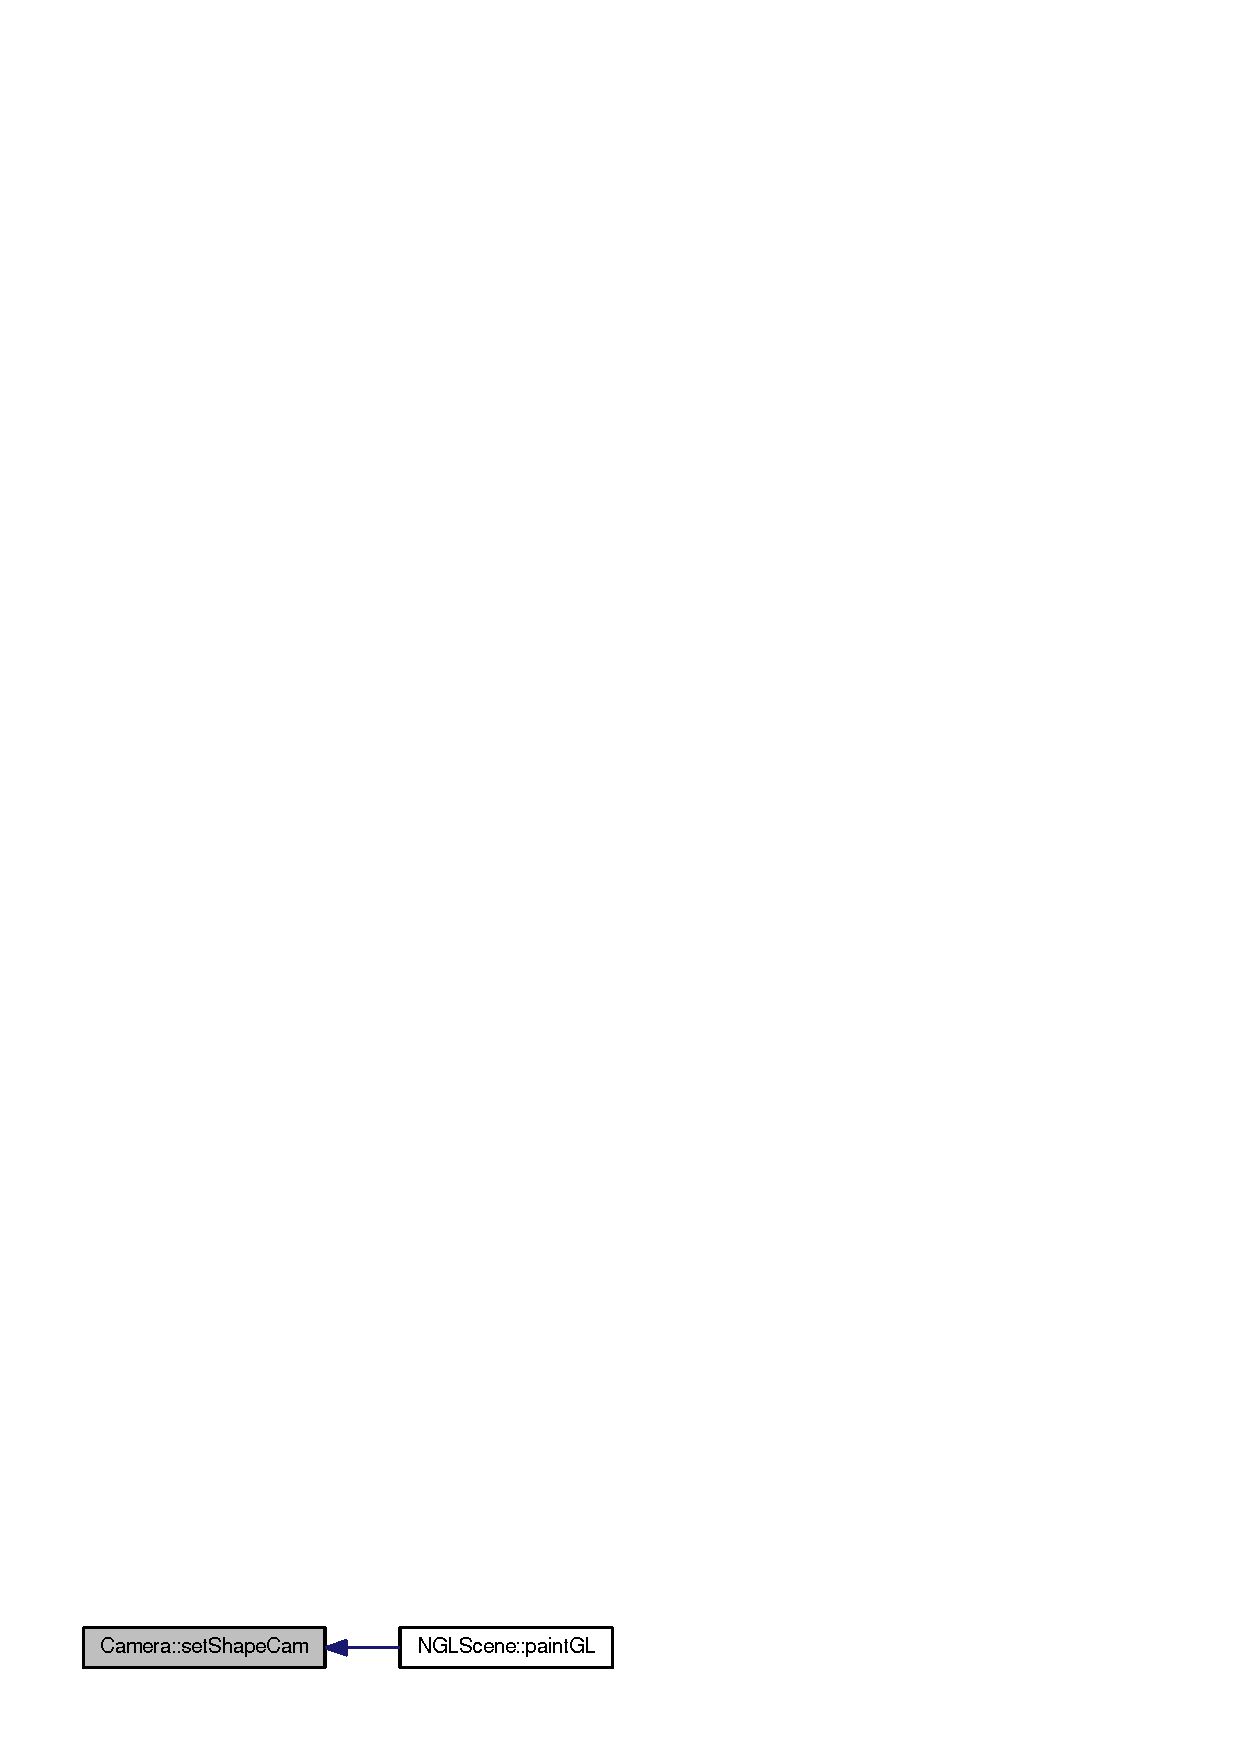
\includegraphics[width=298pt]{class_camera_af155b670c737578ef6e49f9284a1f382_icgraph}
\end{center}
\end{figure}


\index{Camera@{Camera}!update\-Signal@{update\-Signal}}
\index{update\-Signal@{update\-Signal}!Camera@{Camera}}
\subsubsection[{update\-Signal}]{\setlength{\rightskip}{0pt plus 5cm}void Camera\-::update\-Signal (
\begin{DoxyParamCaption}
{}
\end{DoxyParamCaption}
)\hspace{0.3cm}{\ttfamily [signal]}}\label{class_camera_a5274db5a5d8ec834658d5ae5545175b6}


Signal sent to \doxyref{N\-G\-L\-Scene}{p.}{class_n_g_l_scene} update() function to update the scene with the new camera. 



Here is the caller graph for this function\-:\nopagebreak
\begin{figure}[H]
\begin{center}
\leavevmode
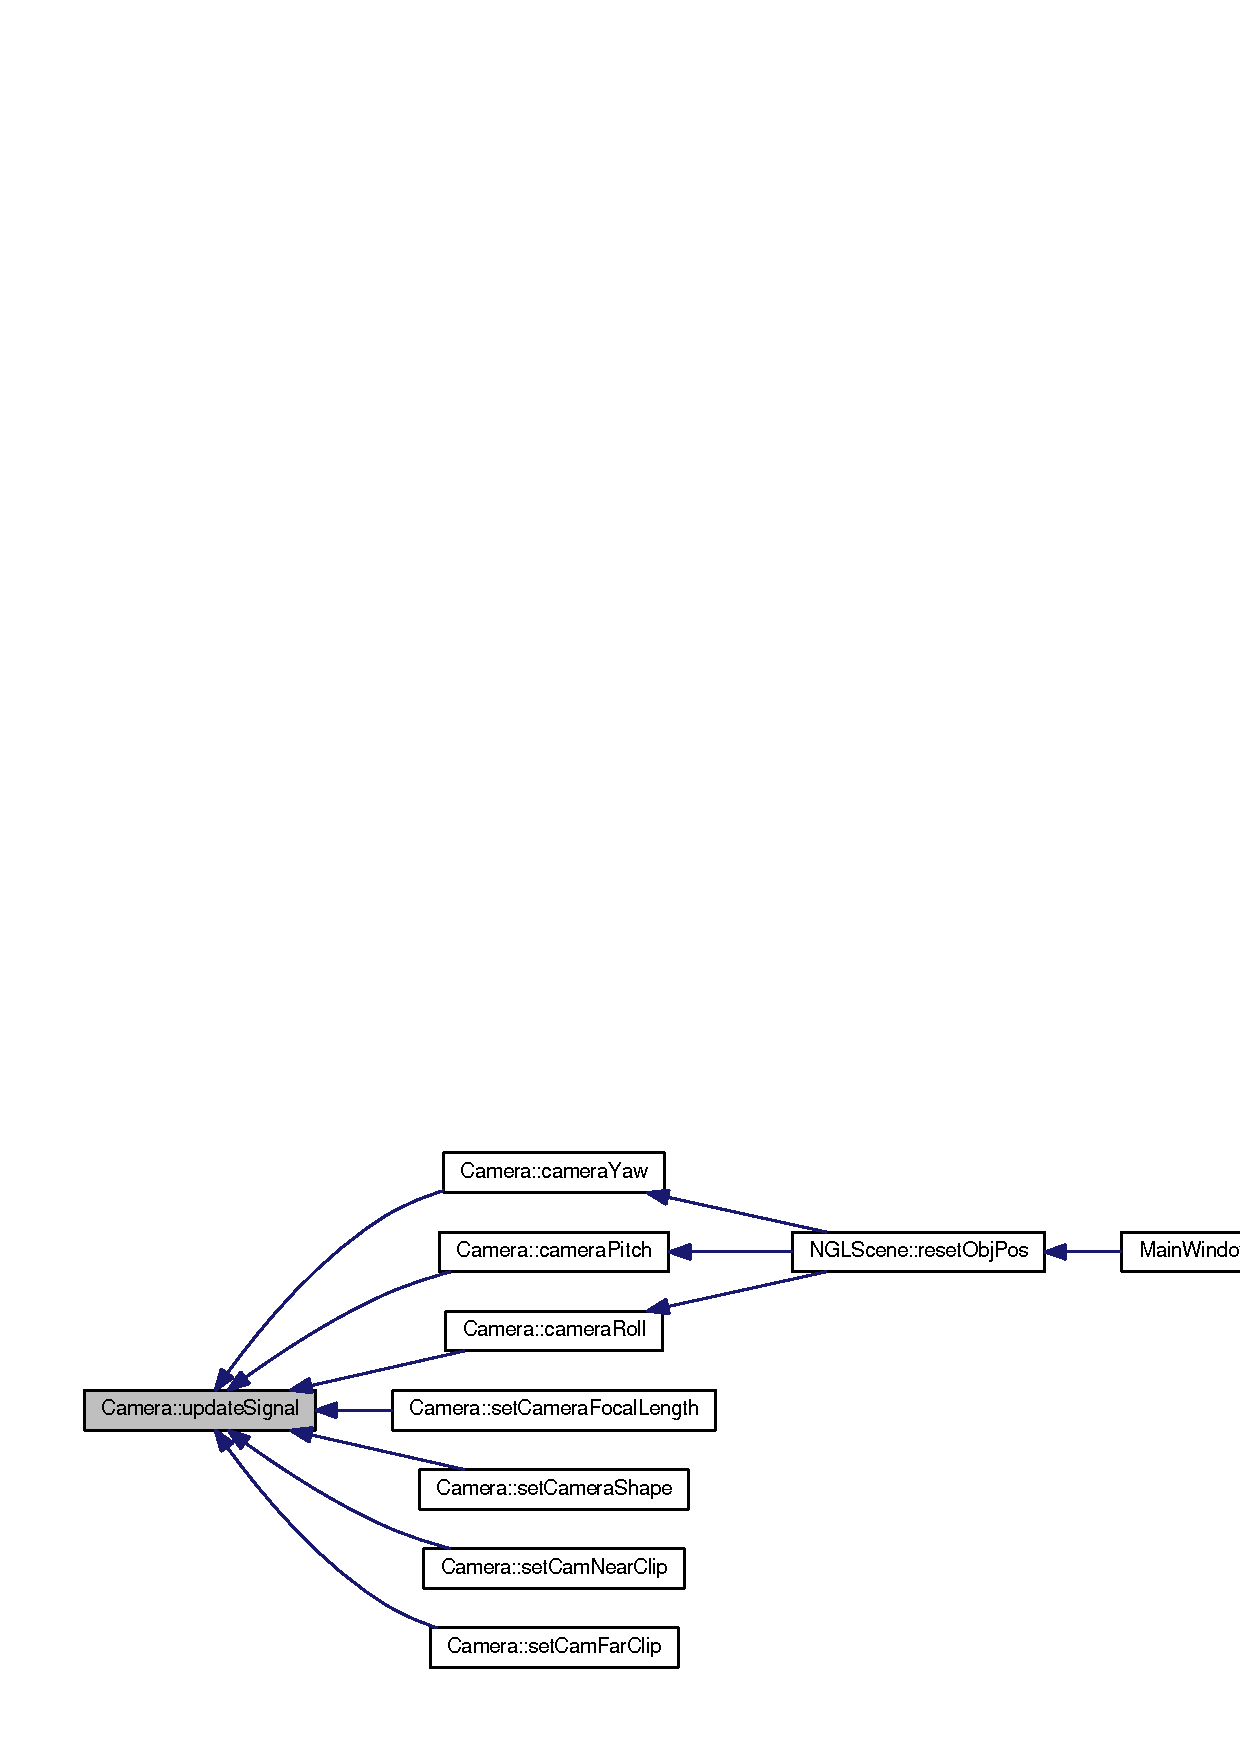
\includegraphics[width=350pt]{class_camera_a5274db5a5d8ec834658d5ae5545175b6_icgraph}
\end{center}
\end{figure}




\subsection{Member Data Documentation}
\index{Camera@{Camera}!m\-\_\-aspect@{m\-\_\-aspect}}
\index{m\-\_\-aspect@{m\-\_\-aspect}!Camera@{Camera}}
\subsubsection[{m\-\_\-aspect}]{\setlength{\rightskip}{0pt plus 5cm}float Camera\-::m\-\_\-aspect}\label{class_camera_abf58e1558e08e785c929f41b25615c30}


aspect ratio of the camera 



Definition at line 49 of file Camera.\-h.

\index{Camera@{Camera}!m\-\_\-camera\-Index@{m\-\_\-camera\-Index}}
\index{m\-\_\-camera\-Index@{m\-\_\-camera\-Index}!Camera@{Camera}}
\subsubsection[{m\-\_\-camera\-Index}]{\setlength{\rightskip}{0pt plus 5cm}int Camera\-::m\-\_\-camera\-Index}\label{class_camera_a6b78f4f27d16a6f97e9d1af12dd52408}


An index to access the cameras. 



Definition at line 41 of file Camera.\-h.

\index{Camera@{Camera}!m\-\_\-camera\-Pitch@{m\-\_\-camera\-Pitch}}
\index{m\-\_\-camera\-Pitch@{m\-\_\-camera\-Pitch}!Camera@{Camera}}
\subsubsection[{m\-\_\-camera\-Pitch}]{\setlength{\rightskip}{0pt plus 5cm}double Camera\-::m\-\_\-camera\-Pitch}\label{class_camera_a2e2a1cbcdc877078e33cab77b032ecd0}


camera pitch value 



Definition at line 69 of file Camera.\-h.

\index{Camera@{Camera}!m\-\_\-camera\-Roll@{m\-\_\-camera\-Roll}}
\index{m\-\_\-camera\-Roll@{m\-\_\-camera\-Roll}!Camera@{Camera}}
\subsubsection[{m\-\_\-camera\-Roll}]{\setlength{\rightskip}{0pt plus 5cm}double Camera\-::m\-\_\-camera\-Roll}\label{class_camera_a84896bffdc7f6657e36cea29f50326d9}


camera roll value 



Definition at line 65 of file Camera.\-h.

\index{Camera@{Camera}!m\-\_\-cameras@{m\-\_\-cameras}}
\index{m\-\_\-cameras@{m\-\_\-cameras}!Camera@{Camera}}
\subsubsection[{m\-\_\-cameras}]{\setlength{\rightskip}{0pt plus 5cm}std\-::vector$<$ngl\-::\-Camera $>$ Camera\-::m\-\_\-cameras}\label{class_camera_a81c3649852e1e6e003fcb6a098b9380b}


A vector containing the ngl cameras. 



Definition at line 37 of file Camera.\-h.

\index{Camera@{Camera}!m\-\_\-camera\-Yaw@{m\-\_\-camera\-Yaw}}
\index{m\-\_\-camera\-Yaw@{m\-\_\-camera\-Yaw}!Camera@{Camera}}
\subsubsection[{m\-\_\-camera\-Yaw}]{\setlength{\rightskip}{0pt plus 5cm}double Camera\-::m\-\_\-camera\-Yaw}\label{class_camera_a84f178ff122318d5f5b3eedfe7a44820}


camera yaw value 



Definition at line 61 of file Camera.\-h.

\index{Camera@{Camera}!m\-\_\-far\-Clip@{m\-\_\-far\-Clip}}
\index{m\-\_\-far\-Clip@{m\-\_\-far\-Clip}!Camera@{Camera}}
\subsubsection[{m\-\_\-far\-Clip}]{\setlength{\rightskip}{0pt plus 5cm}float Camera\-::m\-\_\-far\-Clip}\label{class_camera_ad74bb952b7fc87a3a9e92069ac58cce7}


Far clipping plane of the camera. 



Definition at line 57 of file Camera.\-h.

\index{Camera@{Camera}!m\-\_\-fov@{m\-\_\-fov}}
\index{m\-\_\-fov@{m\-\_\-fov}!Camera@{Camera}}
\subsubsection[{m\-\_\-fov}]{\setlength{\rightskip}{0pt plus 5cm}int Camera\-::m\-\_\-fov}\label{class_camera_aa184f4c3a950d83690a3f2278b64f39e}


fov value for the camera 



Definition at line 45 of file Camera.\-h.

\index{Camera@{Camera}!m\-\_\-main\-Camera@{m\-\_\-main\-Camera}}
\index{m\-\_\-main\-Camera@{m\-\_\-main\-Camera}!Camera@{Camera}}
\subsubsection[{m\-\_\-main\-Camera}]{\setlength{\rightskip}{0pt plus 5cm}ngl\-::\-Camera Camera\-::m\-\_\-main\-Camera}\label{class_camera_a79622becea7694b0f1816789a9c03465}


Active camera used by \doxyref{N\-G\-L\-Scene}{p.}{class_n_g_l_scene}. 



Definition at line 73 of file Camera.\-h.

\index{Camera@{Camera}!m\-\_\-near\-Clip@{m\-\_\-near\-Clip}}
\index{m\-\_\-near\-Clip@{m\-\_\-near\-Clip}!Camera@{Camera}}
\subsubsection[{m\-\_\-near\-Clip}]{\setlength{\rightskip}{0pt plus 5cm}float Camera\-::m\-\_\-near\-Clip}\label{class_camera_adad400a801f8ce12d0e4fed46976e0cd}


Near clipping plane of the camera. 



Definition at line 53 of file Camera.\-h.



The documentation for this class was generated from the following files\-:\begin{DoxyCompactItemize}
\item 
{\bf Camera.\-h}\item 
{\bf Camera.\-cpp}\end{DoxyCompactItemize}

\section{Ceb\-Application Class Reference}
\label{class_ceb_application}\index{Ceb\-Application@{Ceb\-Application}}


used to handle all the gui's application control flow and errors for the program  




{\ttfamily \#include $<$Ceb\-Application.\-h$>$}



Inheritance diagram for Ceb\-Application\-:\nopagebreak
\begin{figure}[H]
\begin{center}
\leavevmode
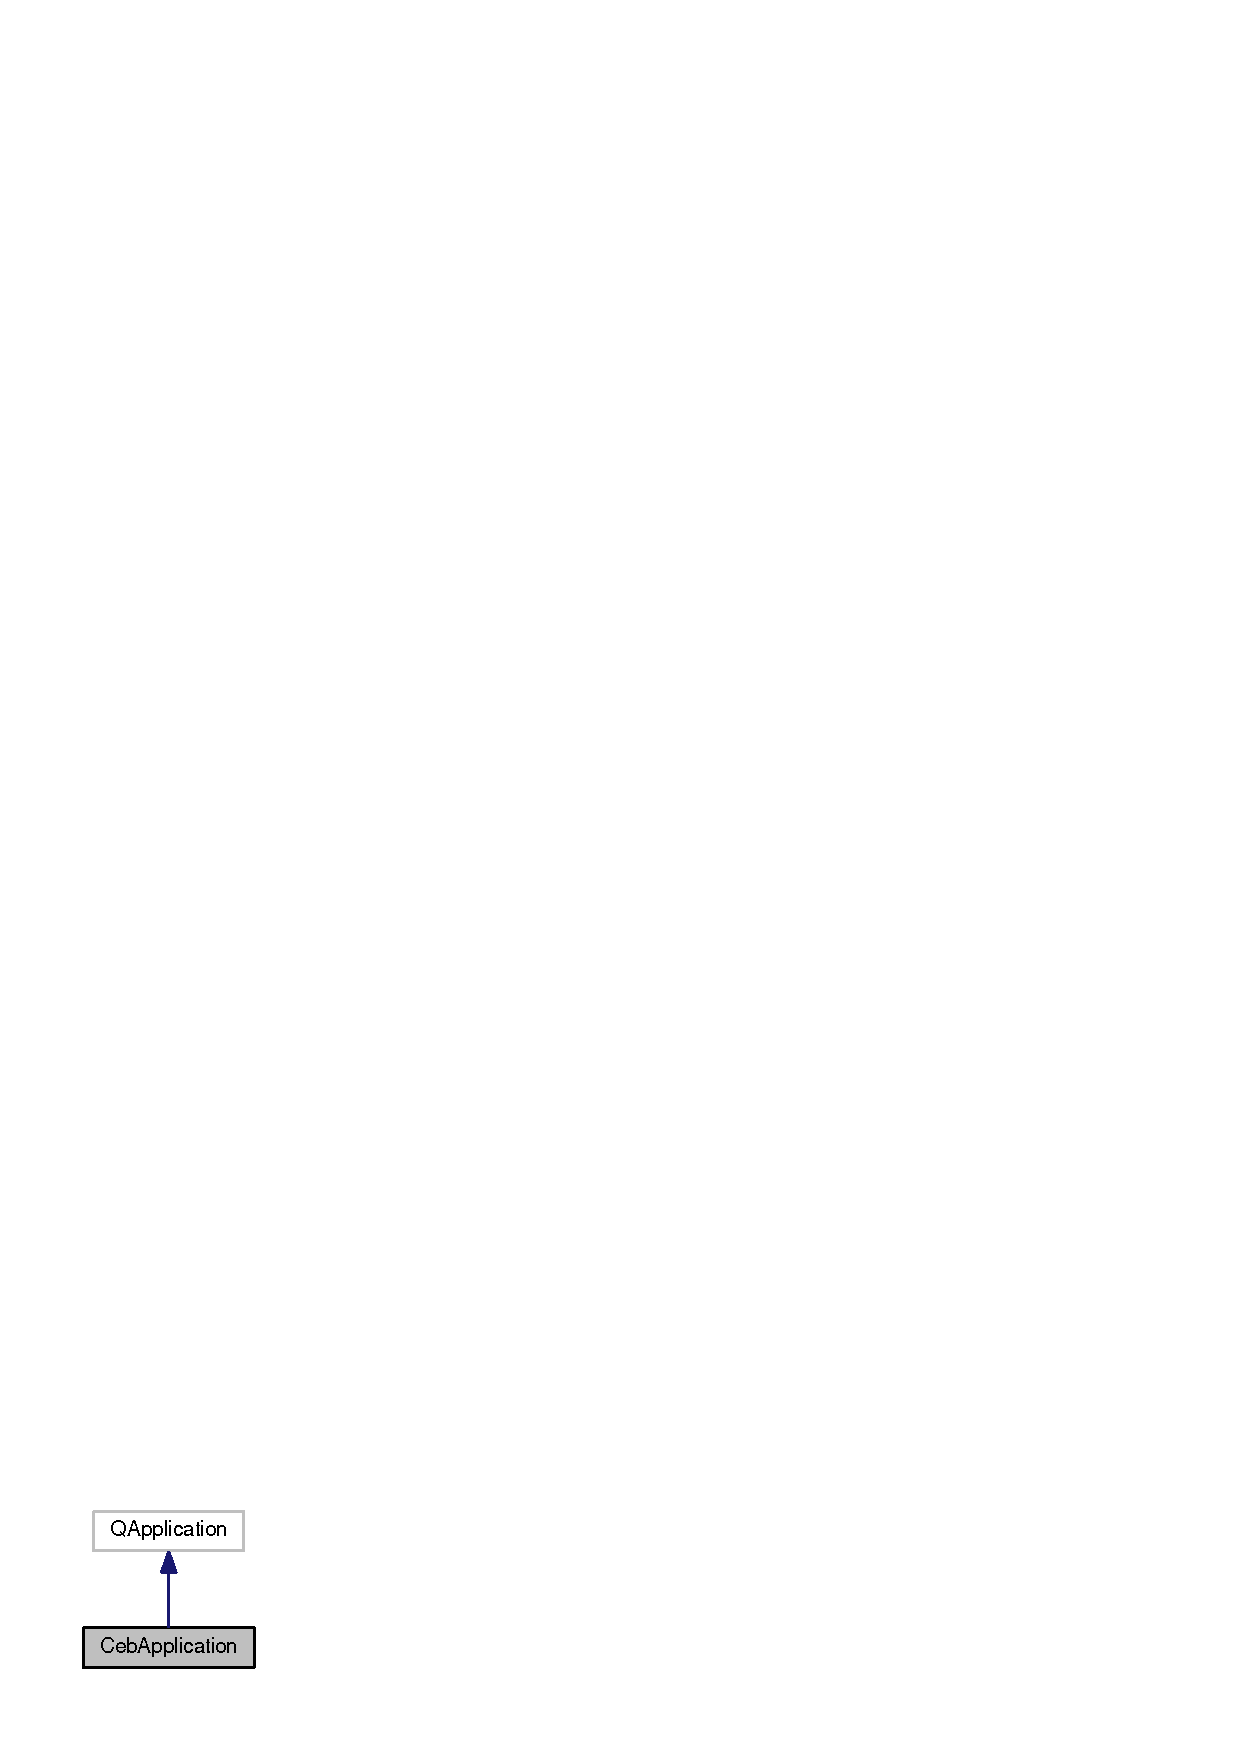
\includegraphics[width=126pt]{class_ceb_application__inherit__graph}
\end{center}
\end{figure}


Collaboration diagram for Ceb\-Application\-:\nopagebreak
\begin{figure}[H]
\begin{center}
\leavevmode
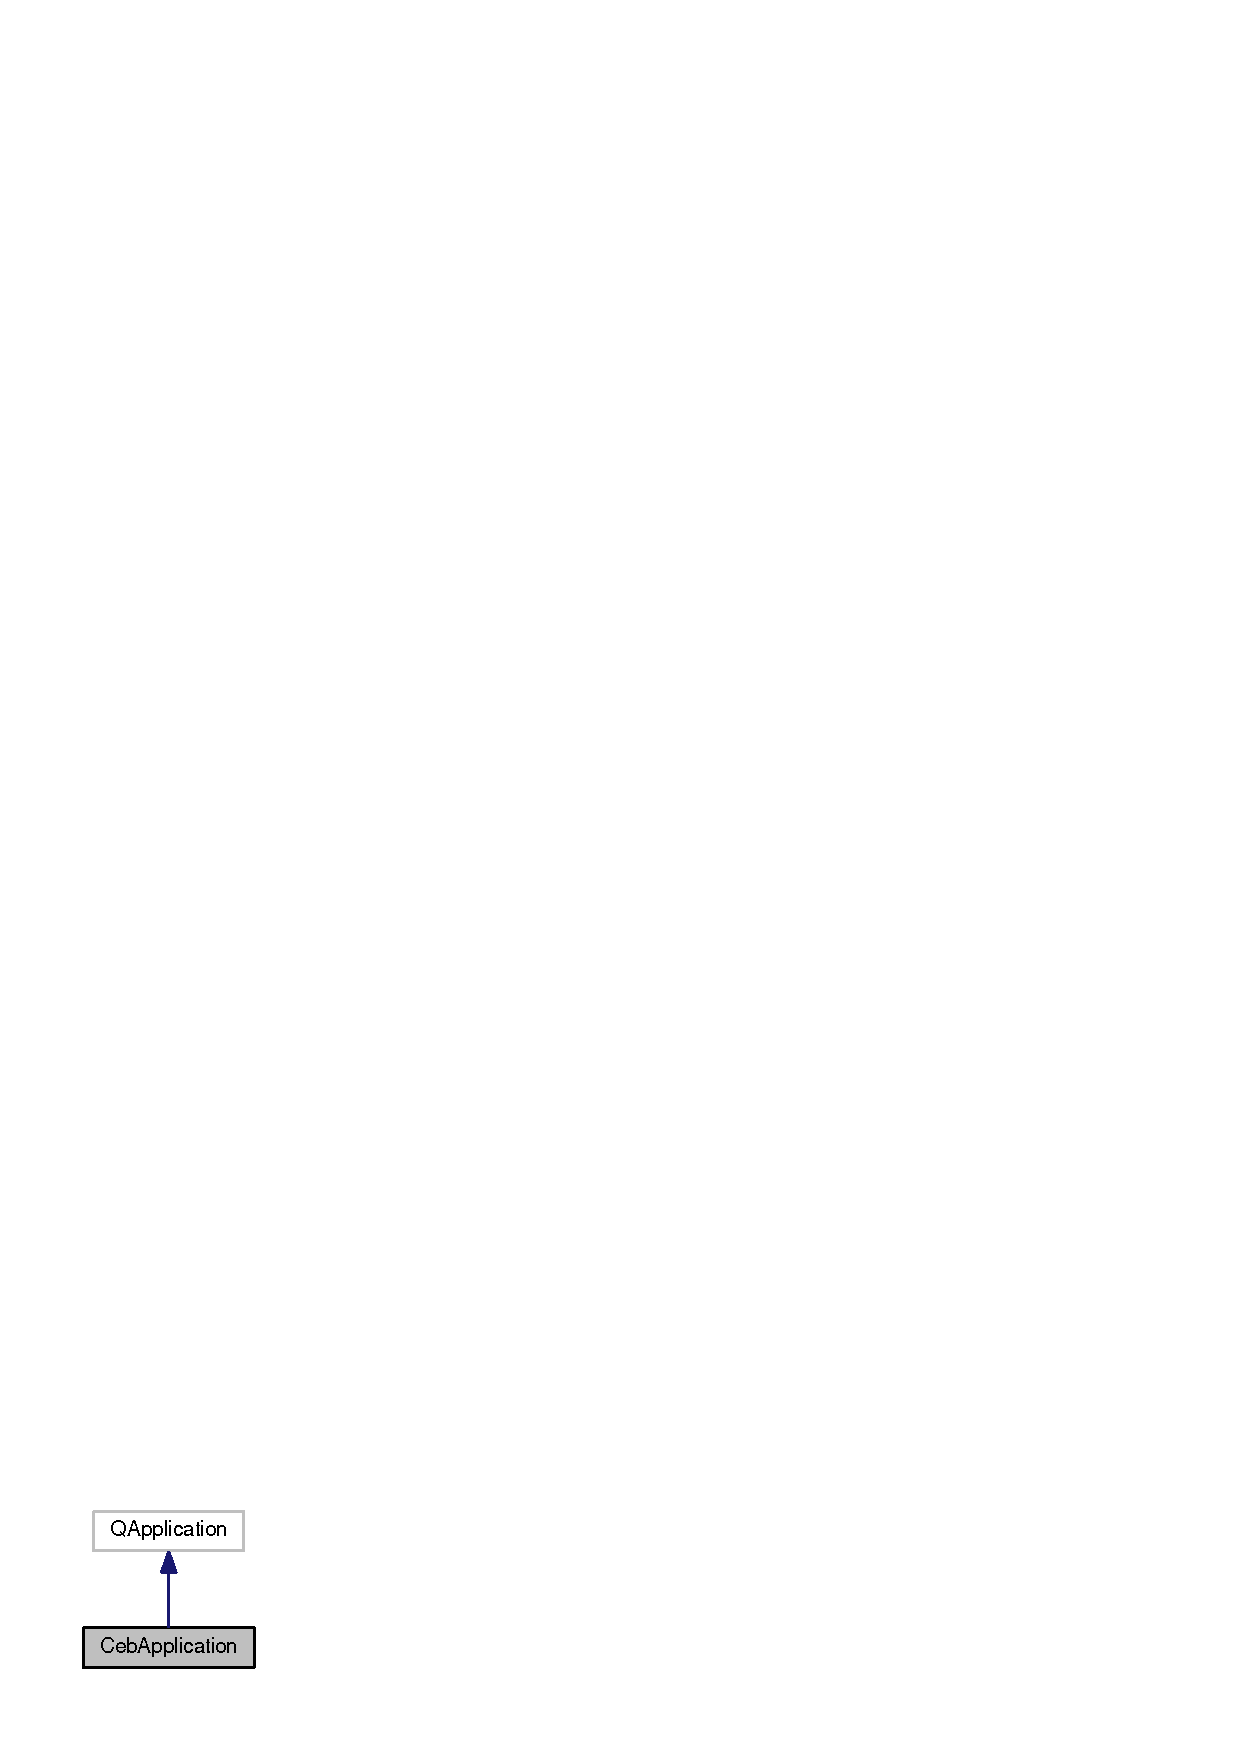
\includegraphics[width=126pt]{class_ceb_application__coll__graph}
\end{center}
\end{figure}
\subsection*{Public Member Functions}
\begin{DoxyCompactItemize}
\item 
bool {\bf notify} (Q\-Object $\ast$\-\_\-reciever, Q\-Event $\ast$\-\_\-event)
\begin{DoxyCompactList}\small\item\em Sends event to receiver and handles errors. Returns the value that is returned from the receiver's event handler or false if error. \end{DoxyCompactList}\end{DoxyCompactItemize}
\subsection*{Public Attributes}
\begin{DoxyCompactItemize}
\item 
Q\-String\-List {\bf m\-\_\-error\-Lvl}
\end{DoxyCompactItemize}
\subsection*{Private Member Functions}
\begin{DoxyCompactItemize}
\item 
Q\-Message\-Box $\ast$ {\bf create\-Error\-Msg\-Box} (std\-::exception $\ast$\-\_\-e, Q\-Object $\ast$\-\_\-reciever, Q\-Event $\ast$\-\_\-event, Q\-Message\-Box\-::\-Icon \-\_\-err\-Lvl)
\begin{DoxyCompactList}\small\item\em creates an error msg created from an exception \end{DoxyCompactList}\end{DoxyCompactItemize}


\subsection{Detailed Description}
used to handle all the gui's application control flow and errors for the program 

Definition at line 30 of file Ceb\-Application.\-h.



\subsection{Member Function Documentation}
\index{Ceb\-Application@{Ceb\-Application}!create\-Error\-Msg\-Box@{create\-Error\-Msg\-Box}}
\index{create\-Error\-Msg\-Box@{create\-Error\-Msg\-Box}!CebApplication@{Ceb\-Application}}
\subsubsection[{create\-Error\-Msg\-Box}]{\setlength{\rightskip}{0pt plus 5cm}Q\-Message\-Box $\ast$ Ceb\-Application\-::create\-Error\-Msg\-Box (
\begin{DoxyParamCaption}
\item[{std\-::exception $\ast$}]{\-\_\-e, }
\item[{Q\-Object $\ast$}]{\-\_\-reciever, }
\item[{Q\-Event $\ast$}]{\-\_\-event, }
\item[{Q\-Message\-Box\-::\-Icon}]{\-\_\-err\-Lvl}
\end{DoxyParamCaption}
)\hspace{0.3cm}{\ttfamily [private]}}\label{class_ceb_application_aa08c777fa24a5889483312b858477926}


creates an error msg created from an exception 


\begin{DoxyParams}[1]{Parameters}
\mbox{\tt in}  & {\em \-\_\-e} & pointer to the exception raised \\
\hline
\mbox{\tt in}  & {\em \-\_\-reciever} & the object that recieves the event \\
\hline
\mbox{\tt in}  & {\em \-\_\-event} & the event that is being sent to the reciever \\
\hline
\mbox{\tt in}  & {\em \-\_\-err\-Lvl} & the error level for the message \\
\hline
\end{DoxyParams}


Definition at line 50 of file Ceb\-Application.\-cpp.



References m\-\_\-error\-Lvl.


\begin{DoxyCode}
54 \{
55   \textcolor{comment}{// Create text and window title message}
56   QString msg = QString(\textcolor{stringliteral}{"%1 Error"}).arg(m_errorLvl[static\_cast<int>(\_errLvl)]);
57   \textcolor{comment}{// Create informative text message}
58   QString iMsg = QString(\_e->what());
59   \textcolor{comment}{// create de}
60   QString dMsg = QString(\textcolor{stringliteral}{"Sending event '%1' to object '%2' (%3)"})
61       .arg(\textcolor{keyword}{typeid}(*\_event).name(),
62            qPrintable(\_reciever->objectName()),
63            \textcolor{keyword}{typeid}(*\_reciever).name());
64 
65   \textcolor{comment}{// Output to console for extra logging}
66   std::cerr << msg.toUtf8().constData() << std::endl
67             << iMsg.toUtf8().constData() << std::endl;
68 
69   \textcolor{comment}{// Create the msgbox}
70   QMessageBox* msgBox = \textcolor{keyword}{new} QMessageBox;
71   \textcolor{comment}{// Set values}
72   msgBox->setIcon(\_errLvl);
73   msgBox->setText(msg);
74   msgBox->setWindowTitle(msg);
75   msgBox->setInformativeText(iMsg);
76   msgBox->setDetailedText(dMsg);
77 
78   \textcolor{keywordflow}{return} msgBox;
79 \}
\end{DoxyCode}


Here is the caller graph for this function\-:\nopagebreak
\begin{figure}[H]
\begin{center}
\leavevmode
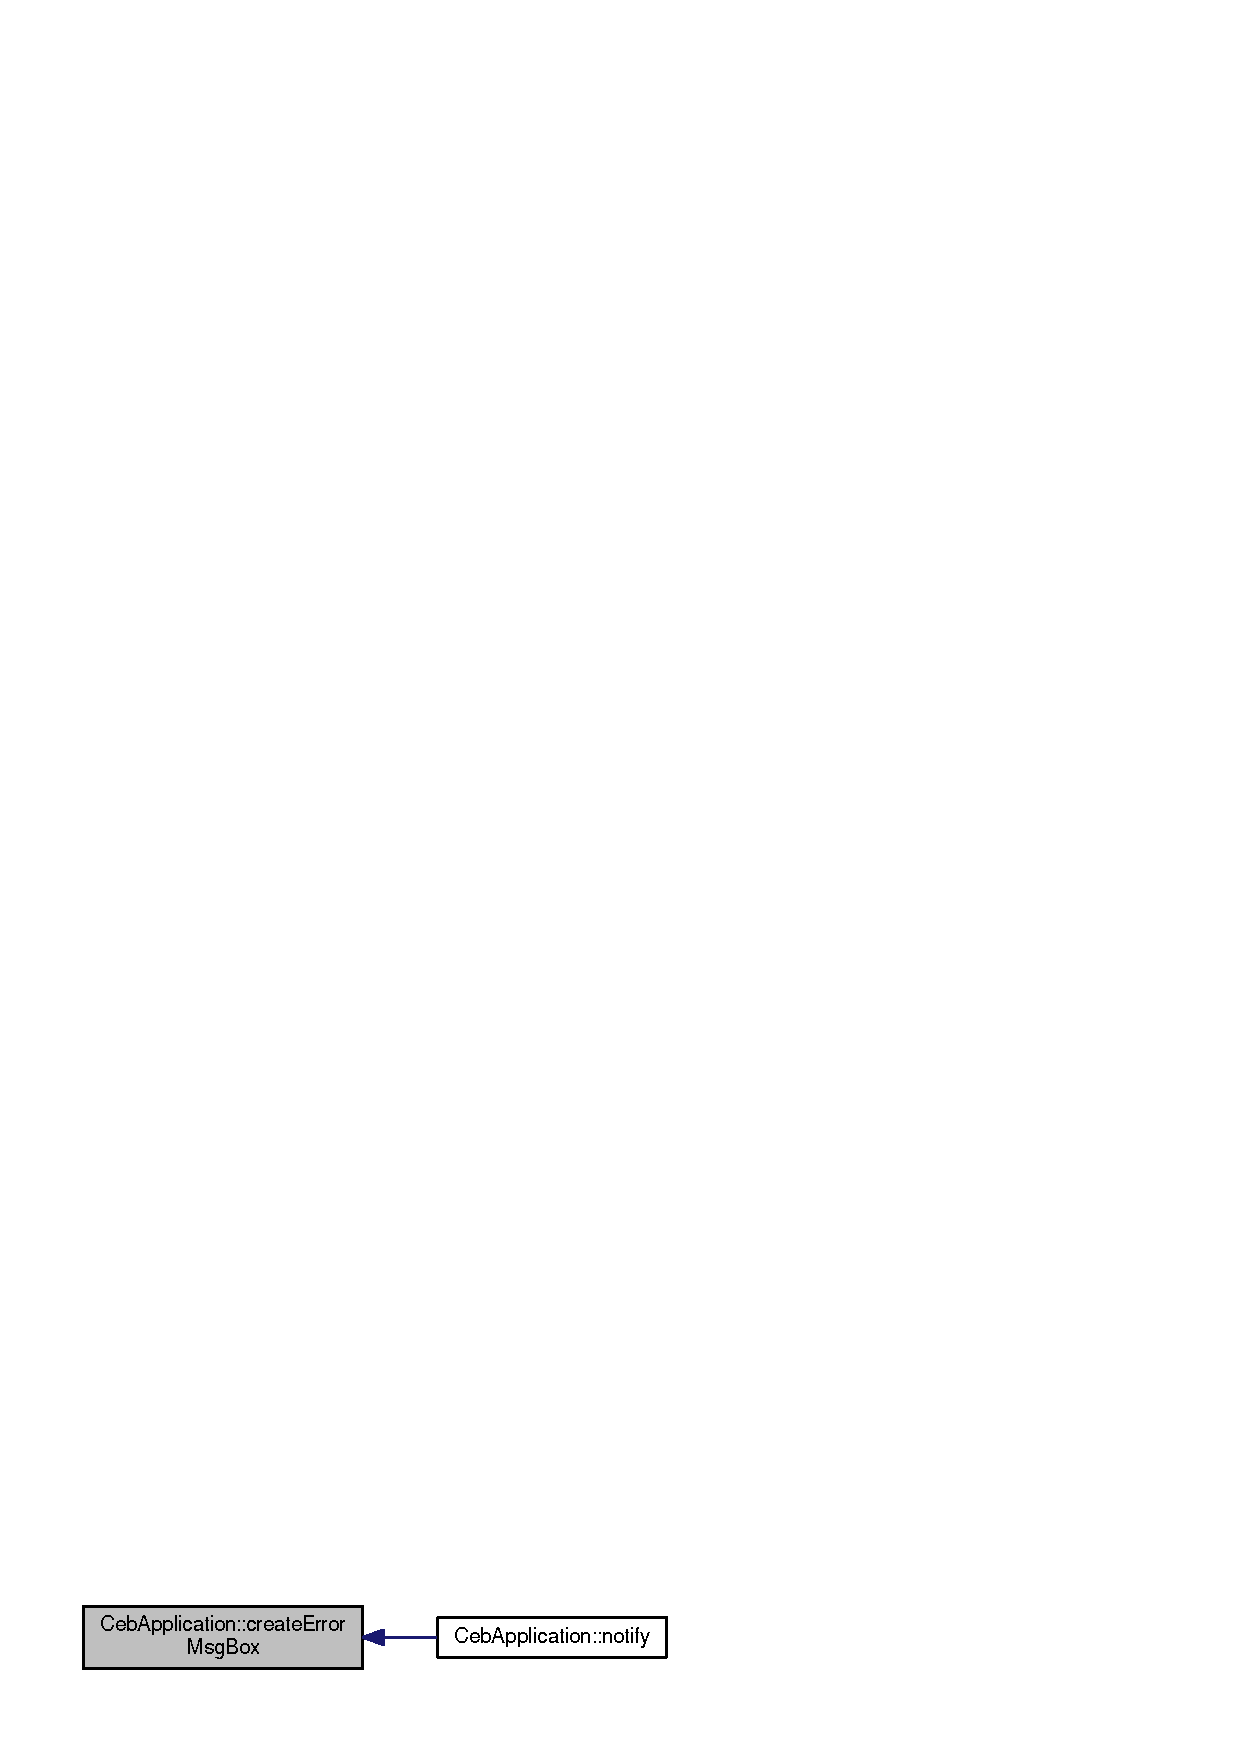
\includegraphics[width=324pt]{class_ceb_application_aa08c777fa24a5889483312b858477926_icgraph}
\end{center}
\end{figure}


\index{Ceb\-Application@{Ceb\-Application}!notify@{notify}}
\index{notify@{notify}!CebApplication@{Ceb\-Application}}
\subsubsection[{notify}]{\setlength{\rightskip}{0pt plus 5cm}bool Ceb\-Application\-::notify (
\begin{DoxyParamCaption}
\item[{Q\-Object $\ast$}]{\-\_\-reciever, }
\item[{Q\-Event $\ast$}]{\-\_\-event}
\end{DoxyParamCaption}
)}\label{class_ceb_application_ab7e35c7770b6ee5c120429ab96ac6963}


Sends event to receiver and handles errors. Returns the value that is returned from the receiver's event handler or false if error. 


\begin{DoxyParams}[1]{Parameters}
\mbox{\tt in}  & {\em \-\_\-reciever} & the object that recieves the event \\
\hline
\mbox{\tt in}  & {\em \-\_\-event} & the event that is being sent to the reciever \\
\hline
\end{DoxyParams}
\begin{DoxyReturn}{Returns}
true if the notify was successful else false 
\end{DoxyReturn}


Definition at line 20 of file Ceb\-Application.\-cpp.



References create\-Error\-Msg\-Box().


\begin{DoxyCode}
21 \{
22   \textcolor{keywordflow}{try} \textcolor{comment}{// Try to notify but will catch an exception if it fails}
23   \{
24     \textcolor{keywordflow}{return} QApplication::notify(\_reciever, \_event);
25   \}
26   \textcolor{keywordflow}{catch} (std::exception &e)
27   \{
28     \textcolor{comment}{// Create and show messagebox}
29     QMessageBox* mBox = createErrorMsgBox(&e, \_reciever, \_event,
30                                           QMessageBox::Critical);
31     mBox->exec();
32 
33     \textcolor{keyword}{delete} mBox;
34   \}
35   \textcolor{keywordflow}{catch} (...)
36   \{
37     \textcolor{comment}{// Create unknown error message then create and show messagebox}
38     CEBError::unknownError e = CEBError::unknownError();
39     QMessageBox* mBox = createErrorMsgBox(&e, \_reciever, \_event,
40                                           QMessageBox::Critical);
41     mBox->exec();
42 
43     \textcolor{keyword}{delete} mBox;
44   \}
45 
46   \textcolor{keywordflow}{return} \textcolor{keyword}{false};
47 \}
\end{DoxyCode}


Here is the call graph for this function\-:\nopagebreak
\begin{figure}[H]
\begin{center}
\leavevmode
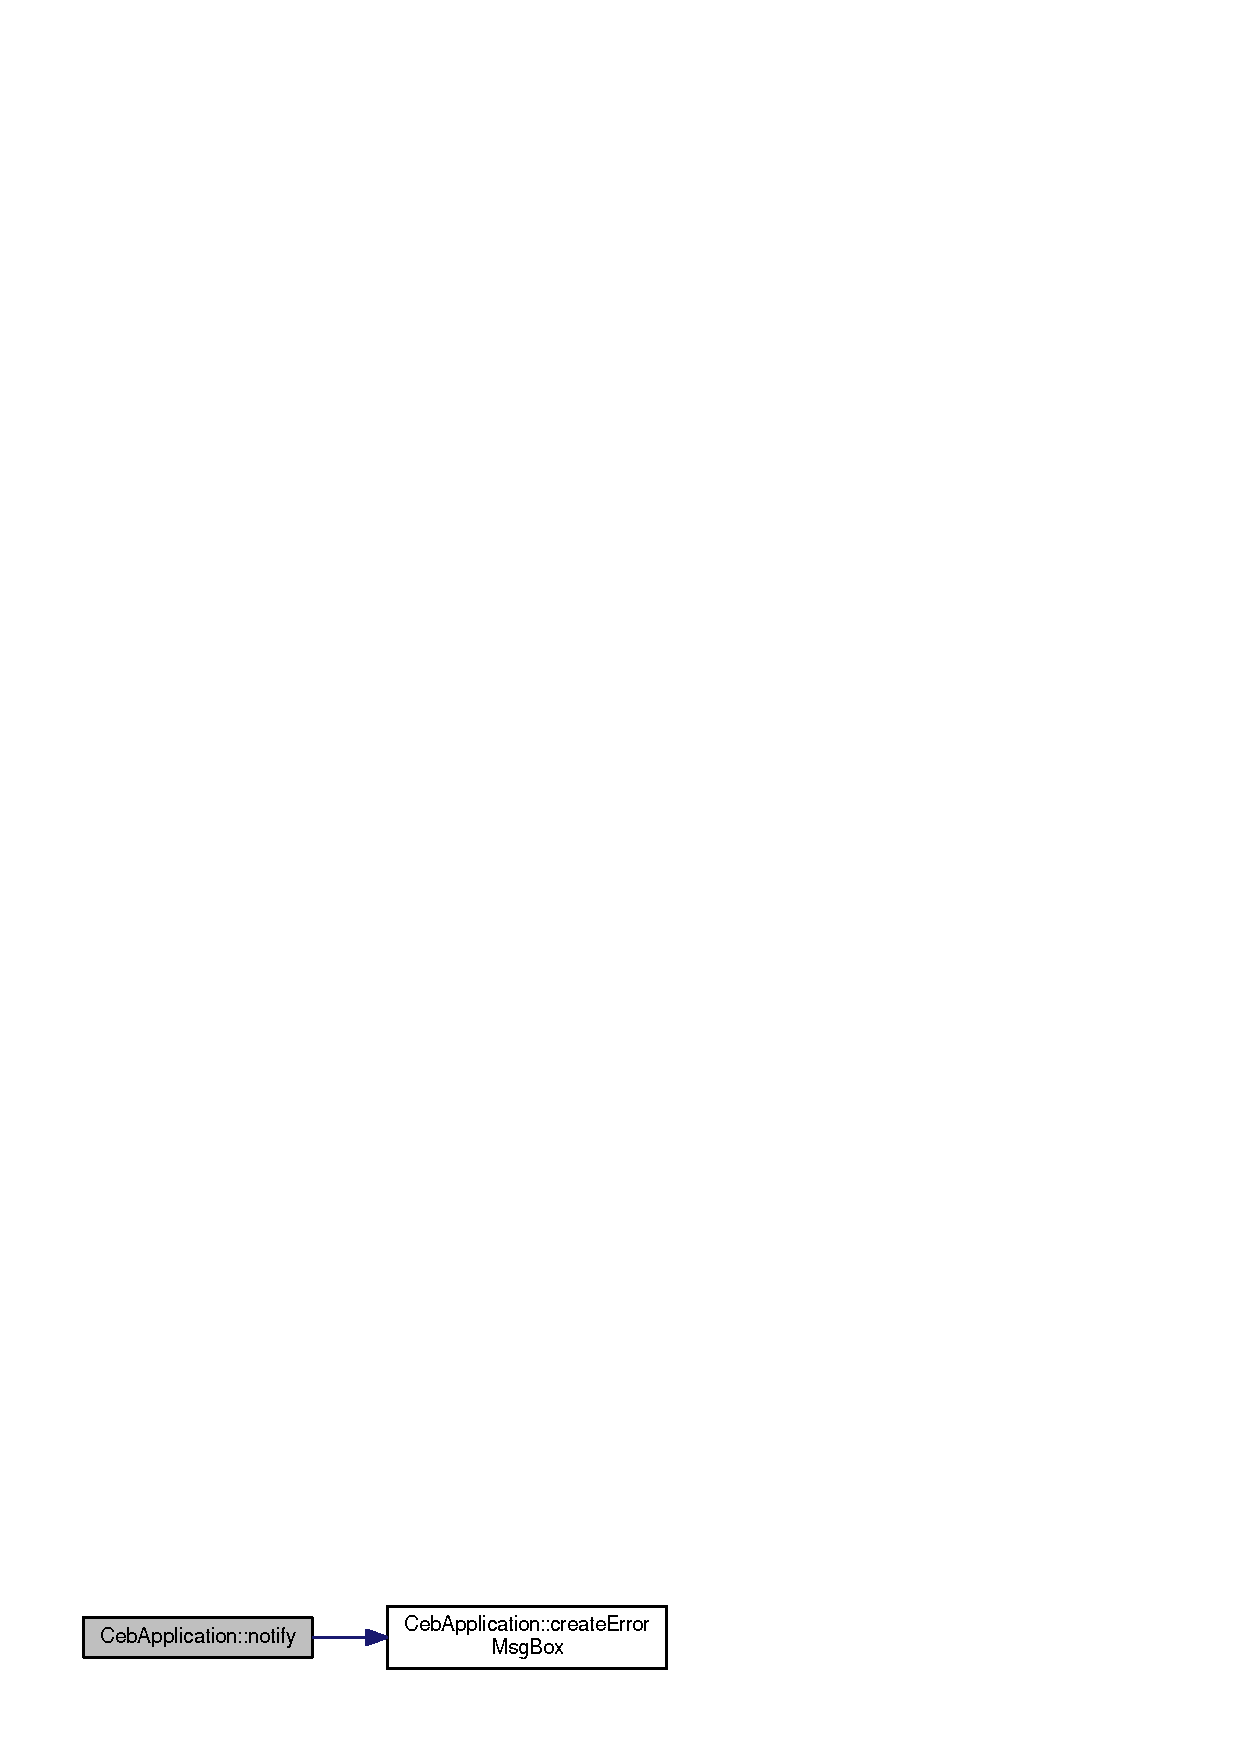
\includegraphics[width=324pt]{class_ceb_application_ab7e35c7770b6ee5c120429ab96ac6963_cgraph}
\end{center}
\end{figure}




\subsection{Member Data Documentation}
\index{Ceb\-Application@{Ceb\-Application}!m\-\_\-error\-Lvl@{m\-\_\-error\-Lvl}}
\index{m\-\_\-error\-Lvl@{m\-\_\-error\-Lvl}!CebApplication@{Ceb\-Application}}
\subsubsection[{m\-\_\-error\-Lvl}]{\setlength{\rightskip}{0pt plus 5cm}Q\-String\-List Ceb\-Application\-::m\-\_\-error\-Lvl}\label{class_ceb_application_a5e62286266b9bff3fd192095faedd1a7}
{\bfseries Initial value\-:}
\begin{DoxyCode}
= \{\textcolor{stringliteral}{"Message"}, \textcolor{stringliteral}{"Information"}, \textcolor{stringliteral}{"Warning"},
                              \textcolor{stringliteral}{"Critical"}, \textcolor{stringliteral}{"Question"}\}
\end{DoxyCode}


Definition at line 38 of file Ceb\-Application.\-h.



The documentation for this class was generated from the following files\-:\begin{DoxyCompactItemize}
\item 
{\bf Ceb\-Application.\-h}\item 
{\bf Ceb\-Application.\-cpp}\end{DoxyCompactItemize}

\section{Cebitor Class Reference}
\label{class_cebitor}\index{Cebitor@{Cebitor}}


C\-E\-B text editor class inherits from Qsci\-Scintilla.  




{\ttfamily \#include $<$Cebitor.\-h$>$}



Inheritance diagram for Cebitor\-:\nopagebreak
\begin{figure}[H]
\begin{center}
\leavevmode
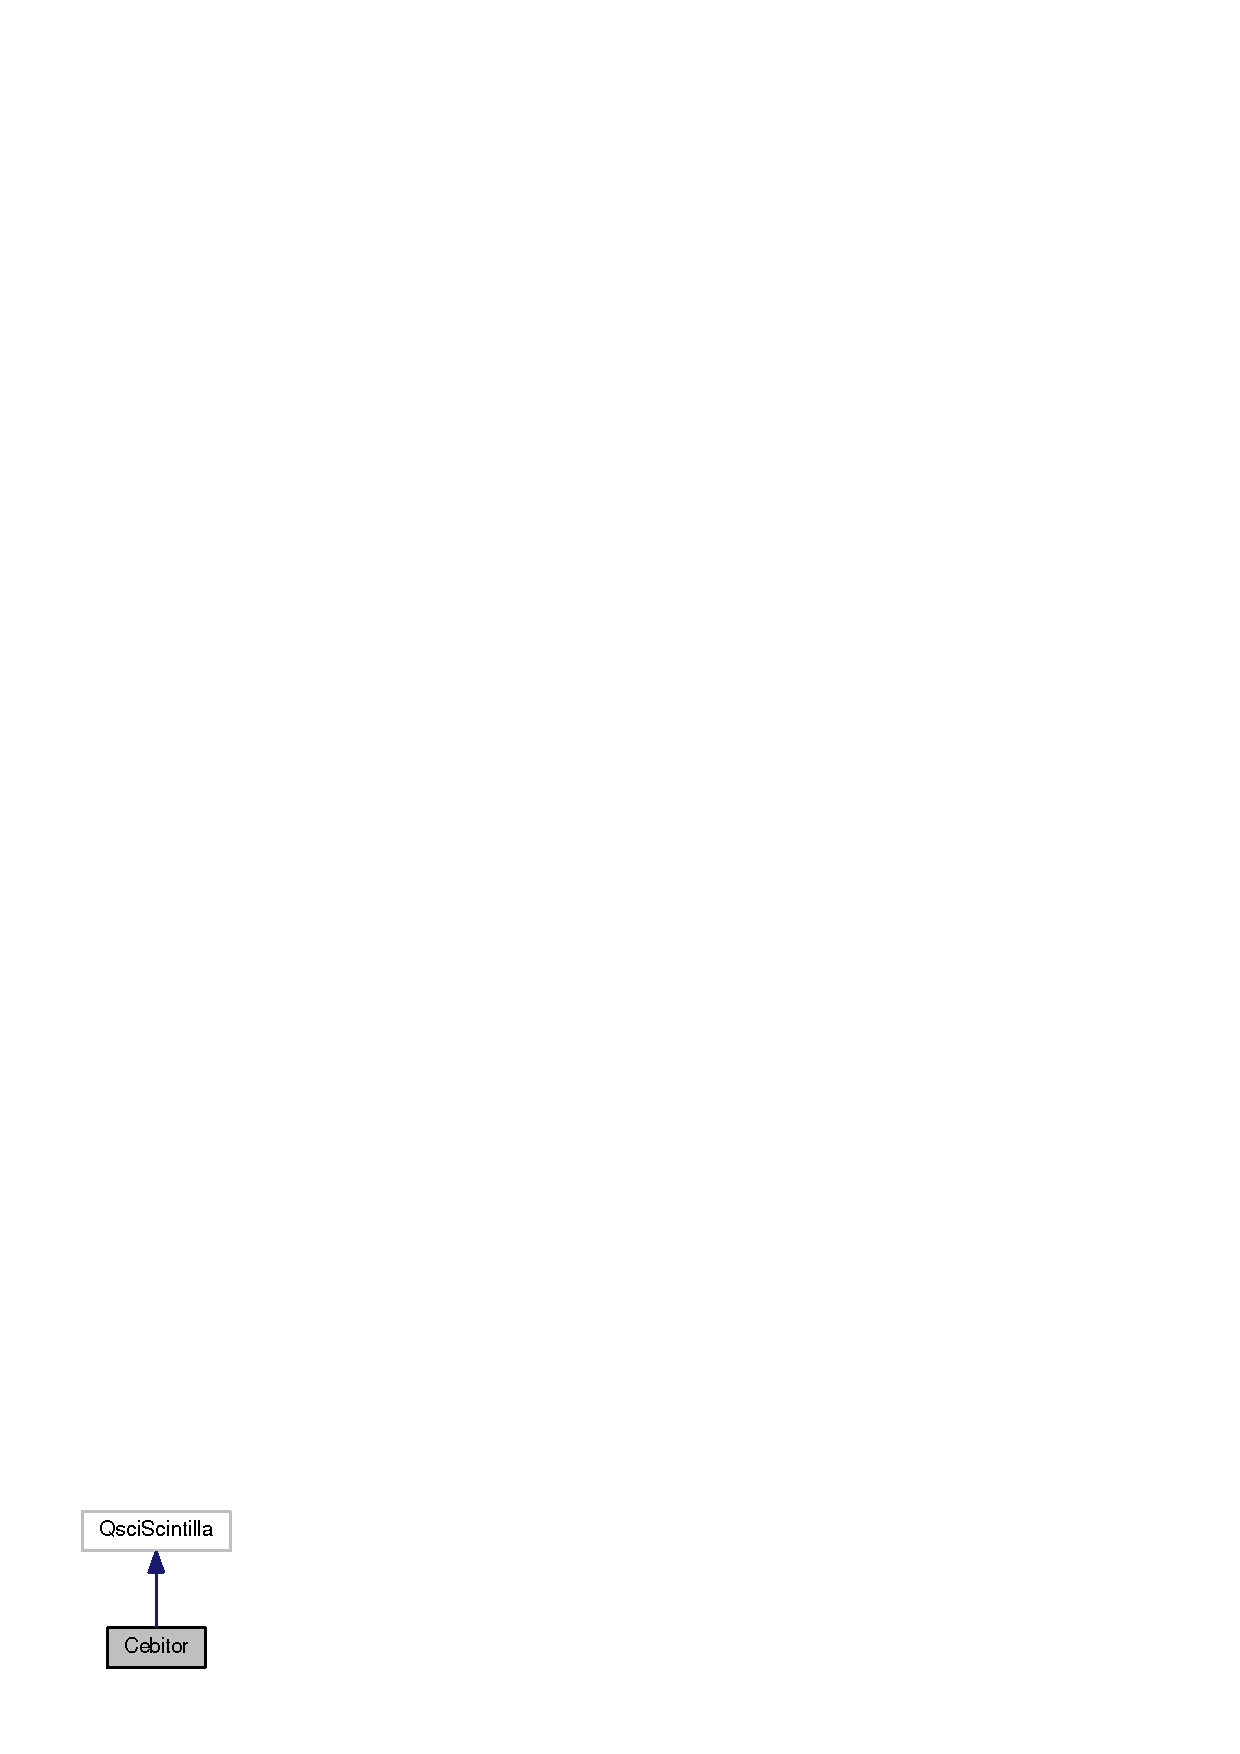
\includegraphics[width=114pt]{class_cebitor__inherit__graph}
\end{center}
\end{figure}


Collaboration diagram for Cebitor\-:\nopagebreak
\begin{figure}[H]
\begin{center}
\leavevmode
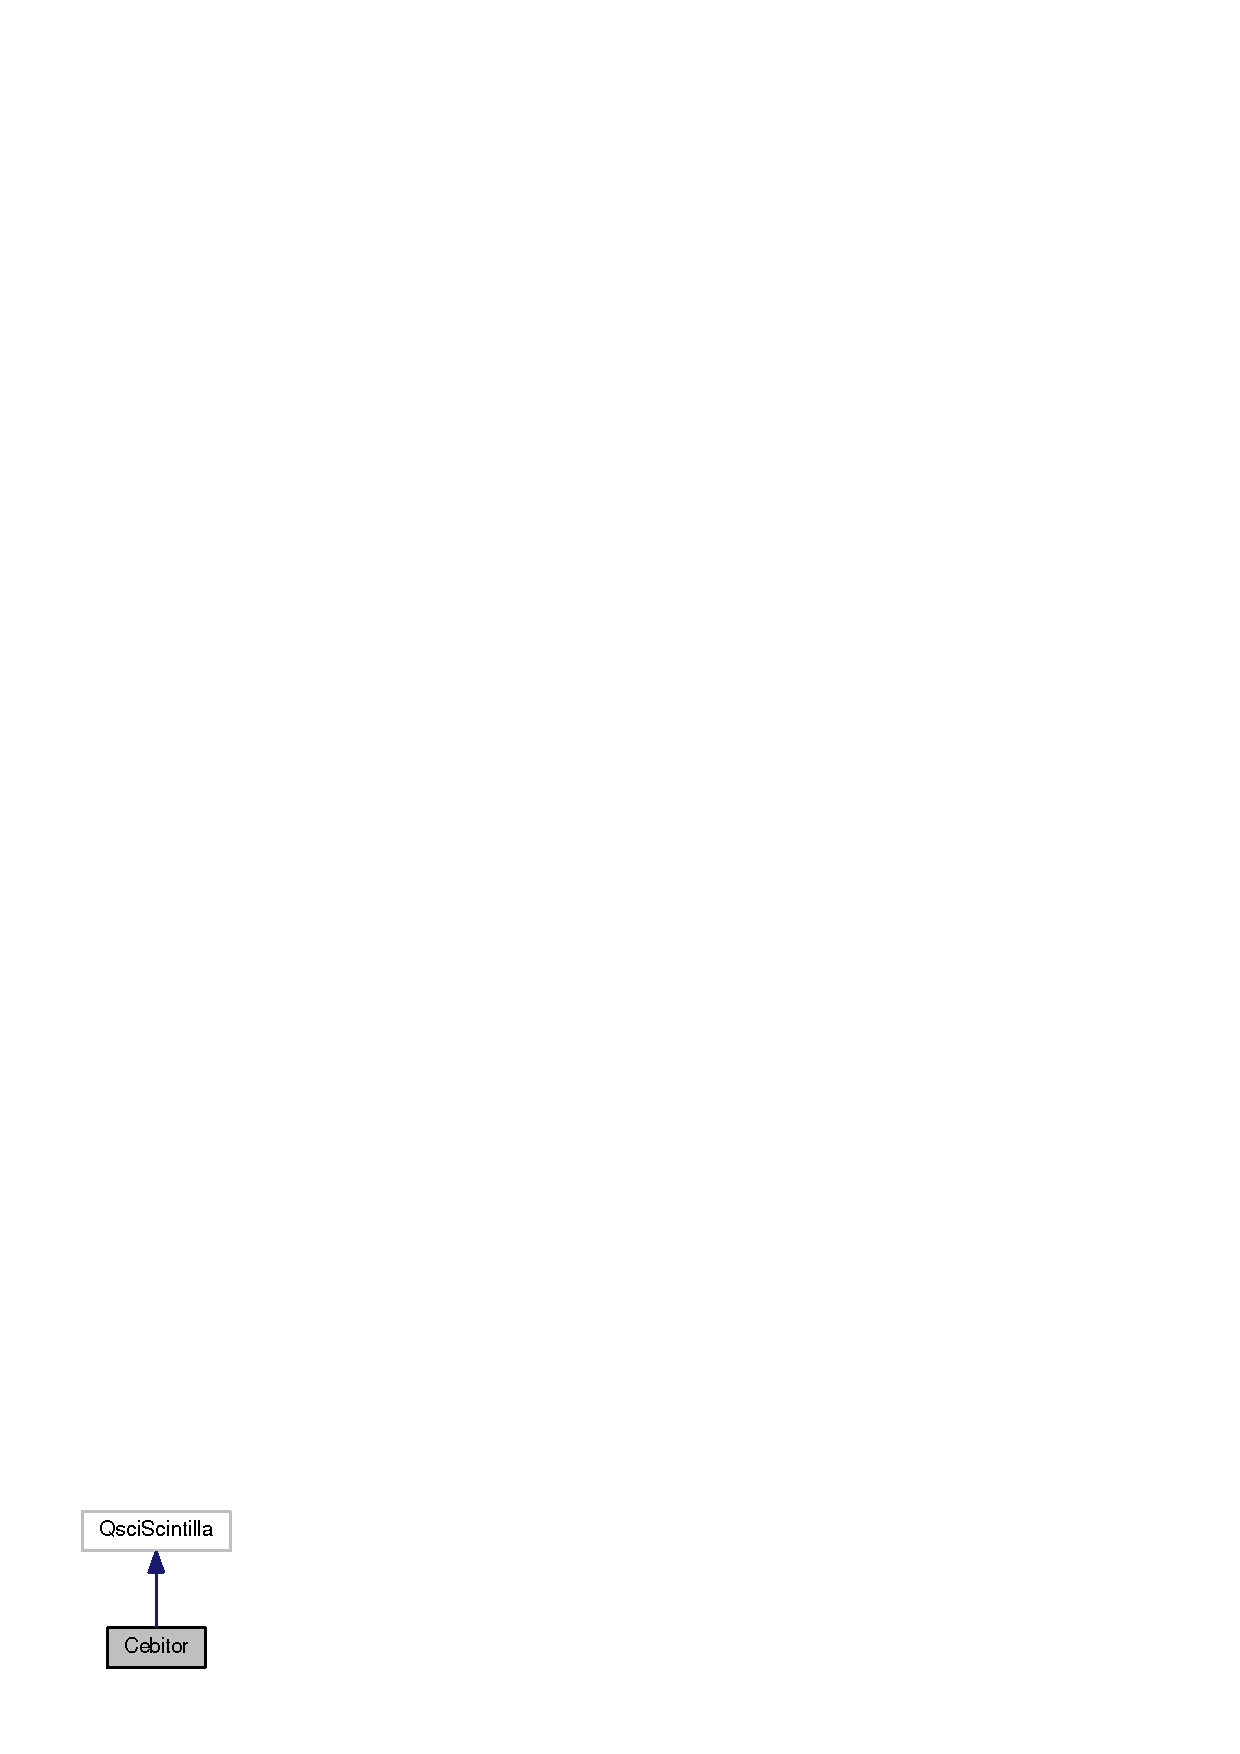
\includegraphics[width=114pt]{class_cebitor__coll__graph}
\end{center}
\end{figure}
\subsection*{Public Types}
\begin{DoxyCompactItemize}
\item 
enum {\bf Marker\-Type} \{ {\bf E\-R\-R\-O\-R}, 
{\bf W\-A\-R\-N\-I\-N\-G}
 \}
\begin{DoxyCompactList}\small\item\em Enum for supported marker types. \end{DoxyCompactList}\end{DoxyCompactItemize}
\subsection*{Public Slots}
\begin{DoxyCompactItemize}
\item 
void {\bf clear\-Errors} ()
\begin{DoxyCompactList}\small\item\em Removes all error and warning line markers. \end{DoxyCompactList}\item 
void {\bf search\-Next} ()
\begin{DoxyCompactList}\small\item\em Search for next occurance. \end{DoxyCompactList}\item 
void {\bf search\-Prev} ()
\begin{DoxyCompactList}\small\item\em Search for previous occurance. \end{DoxyCompactList}\item 
void {\bf highlight\-All\-Search} ()
\begin{DoxyCompactList}\small\item\em sets indicator for each search result \end{DoxyCompactList}\item 
void {\bf highlight\-All\-Search} (const Q\-String \&\-\_\-text)
\begin{DoxyCompactList}\small\item\em sets indicator for each search result \end{DoxyCompactList}\end{DoxyCompactItemize}
\subsection*{Public Member Functions}
\begin{DoxyCompactItemize}
\item 
{\bf Cebitor} (Q\-Widget $\ast$\-\_\-parent)
\begin{DoxyCompactList}\small\item\em \doxyref{Cebitor}{p.}{class_cebitor} constructor, initialises default values. \end{DoxyCompactList}\item 
void {\bf set\-Search\-Widget} (Q\-Widget $\ast$\-\_\-search\-Widget)
\begin{DoxyCompactList}\small\item\em stores widget containing the searchbar \end{DoxyCompactList}\item 
void {\bf set\-Search\-Line\-Edit} (Q\-Line\-Edit $\ast$\-\_\-search\-Line\-Edit)
\begin{DoxyCompactList}\small\item\em stores Q\-Line\-Edit widget from the searchbar \end{DoxyCompactList}\end{DoxyCompactItemize}
\subsection*{Protected Slots}
\begin{DoxyCompactItemize}
\item 
void {\bf comment} ()
\begin{DoxyCompactList}\small\item\em comment out all selected lines \end{DoxyCompactList}\item 
void {\bf toggle\-Search\-Box} ()
\begin{DoxyCompactList}\small\item\em toggle search widget \end{DoxyCompactList}\item 
void {\bf char\-Added} (const int \-\_\-c)
\begin{DoxyCompactList}\small\item\em called when a character is added \end{DoxyCompactList}\item 
void {\bf reset\-Highlight\-Colour} ()
\begin{DoxyCompactList}\small\item\em reset the highlighting colour \end{DoxyCompactList}\end{DoxyCompactItemize}
\subsection*{Protected Member Functions}
\begin{DoxyCompactItemize}
\item 
bool {\bf auto\-Close} (const Q\-String \-\_\-close)
\begin{DoxyCompactList}\small\item\em adds closing character for braces and quotes \end{DoxyCompactList}\item 
bool {\bf closing} (const Q\-String \-\_\-close)
\begin{DoxyCompactList}\small\item\em removes duplicates of closing braces and quotes \end{DoxyCompactList}\item 
void {\bf brace\-Indent} ()
\begin{DoxyCompactList}\small\item\em adds indentation after newline following a \char`\"{}\{\char`\"{} \end{DoxyCompactList}\end{DoxyCompactItemize}
\subsection*{Protected Attributes}
\begin{DoxyCompactItemize}
\item 
Q\-Widget $\ast$ {\bf m\-\_\-search\-Widget}
\begin{DoxyCompactList}\small\item\em widget containing the searchbar \end{DoxyCompactList}\item 
Q\-Line\-Edit $\ast$ {\bf m\-\_\-search\-Line\-Edit}
\begin{DoxyCompactList}\small\item\em searchbar Q\-Line\-Edit widget \end{DoxyCompactList}\item 
std\-::vector$<$ int $>$ {\bf m\-\_\-file\-Markers}
\begin{DoxyCompactList}\small\item\em vector of all line markers \end{DoxyCompactList}\item 
int {\bf m\-\_\-search\-Indicator}
\begin{DoxyCompactList}\small\item\em indicator used to highlight all search terms \end{DoxyCompactList}\end{DoxyCompactItemize}


\subsection{Detailed Description}
C\-E\-B text editor class inherits from Qsci\-Scintilla. 

Definition at line 22 of file Cebitor.\-h.



\subsection{Member Enumeration Documentation}
\index{Cebitor@{Cebitor}!Marker\-Type@{Marker\-Type}}
\index{Marker\-Type@{Marker\-Type}!Cebitor@{Cebitor}}
\subsubsection[{Marker\-Type}]{\setlength{\rightskip}{0pt plus 5cm}enum {\bf Cebitor\-::\-Marker\-Type}}\label{class_cebitor_af43f4242de6e469e6d6c61bdd4093446}


Enum for supported marker types. 

\begin{Desc}
\item[Enumerator]\par
\begin{description}
\index{E\-R\-R\-O\-R@{E\-R\-R\-O\-R}!Cebitor@{Cebitor}}\index{Cebitor@{Cebitor}!E\-R\-R\-O\-R@{E\-R\-R\-O\-R}}\item[{\em 
E\-R\-R\-O\-R\label{class_cebitor_af43f4242de6e469e6d6c61bdd4093446a49f150e78b6812cea262ccb80eebdeb5}
}]Symbol marker for Errors. \index{W\-A\-R\-N\-I\-N\-G@{W\-A\-R\-N\-I\-N\-G}!Cebitor@{Cebitor}}\index{Cebitor@{Cebitor}!W\-A\-R\-N\-I\-N\-G@{W\-A\-R\-N\-I\-N\-G}}\item[{\em 
W\-A\-R\-N\-I\-N\-G\label{class_cebitor_af43f4242de6e469e6d6c61bdd4093446a5d9f8a9512323adcfb3a5586b3867183}
}]Symbol marker for warnings. \end{description}
\end{Desc}


Definition at line 30 of file Cebitor.\-h.


\begin{DoxyCode}
31   \{
32     ERROR,    
33     WARNING,  
34   \};
\end{DoxyCode}


\subsection{Constructor \& Destructor Documentation}
\index{Cebitor@{Cebitor}!Cebitor@{Cebitor}}
\index{Cebitor@{Cebitor}!Cebitor@{Cebitor}}
\subsubsection[{Cebitor}]{\setlength{\rightskip}{0pt plus 5cm}Cebitor\-::\-Cebitor (
\begin{DoxyParamCaption}
\item[{Q\-Widget $\ast$}]{\-\_\-parent}
\end{DoxyParamCaption}
)}\label{class_cebitor_a8295f41644184b799f7c0165627f391a}


\doxyref{Cebitor}{p.}{class_cebitor} constructor, initialises default values. 

\begin{DoxyRefDesc}{Bug}
\item[{\bf Bug}]brace matching matches \char`\"{}$<$\char`\"{} and \char`\"{}$>$\char`\"{} characters \end{DoxyRefDesc}


Definition at line 23 of file Cebitor.\-cpp.



References char\-Added(), comment(), m\-\_\-search\-Indicator, reset\-Highlight\-Colour(), and toggle\-Search\-Box().


\begin{DoxyCode}
23                                  : QsciScintilla(\_parent)
24 \{
25   setMinimumHeight(300);
26 
27   \textcolor{comment}{// Create and assign the lexer}
28   QsciLexer* lex = \textcolor{keyword}{new} QsciLexerGLSL(\textcolor{keyword}{this});
29   setLexer(lex);
30 
31   \textcolor{comment}{// Set the margin defaults}
32   setMarginType(0,MarginType::NumberMargin);
33   setMarginWidth(0,\textcolor{stringliteral}{" 012"});
34   setMarginsForegroundColor(QColor(128, 128, 128));
35   \textcolor{comment}{// Set the symbol margin defaults}
36   setMarginType(1,MarginType::SymbolMargin);
37   setMarginWidth(1,12);
38   setMarginMarkerMask(1,
39                       1 << MarkerType::ERROR |
40                       1 << MarkerType::WARNING
41                       );
42 
43   \textcolor{comment}{// Set the caret defaults}
44   setCaretForegroundColor(QColor(247, 247, 241));
45   setCaretWidth(2);
46   \textcolor{comment}{// Set the brace defaults}
47   \textcolor{comment}{//----------------------------------------------------------------------------}
49 \textcolor{comment}{}  \textcolor{comment}{//----------------------------------------------------------------------------}
50   setBraceMatching(BraceMatch::SloppyBraceMatch);
51   setMatchedBraceBackgroundColor(QColor(62, 61, 50));
52   setUnmatchedBraceBackgroundColor(QColor(249, 38, 114));
53 
54   \textcolor{comment}{// Set auto-indent}
55   setAutoIndent(\textcolor{keyword}{true});
56   setIndentationsUseTabs(\textcolor{keyword}{false});
57   setIndentationWidth(2);
58 
59   \textcolor{comment}{// Enable scroll width tracking and set the scroll width to a low number}
60   \textcolor{comment}{// Scintilla doesn't track line length, so if we wanted automated scrollbar}
61   \textcolor{comment}{// to appear we would need to implement a line length checking}
62   SendScintilla(QsciScintillaBase::SCI\_SETSCROLLWIDTHTRACKING, 1);
63   SendScintilla(QsciScintillaBase::SCI\_SETSCROLLWIDTH, 5);
64 
65   \textcolor{comment}{// set up line markers}
66   QIcon errorIcon = QIcon::fromTheme(QString(\textcolor{stringliteral}{"dialog-error"}));
67   QIcon warnIcon = QIcon::fromTheme(QString(\textcolor{stringliteral}{"dialog-warning"}));
68 
69   markerDefine(errorIcon.pixmap(10,10), MarkerType::ERROR);
70   markerDefine(warnIcon.pixmap(10,10), MarkerType::WARNING);
71 
72   \textcolor{comment}{// unbind CTRL-/ keyboard shortcut}
73   standardCommands()->boundTo(Qt::Key\_Slash | Qt::CTRL)->setKey(0);
74 
75   \textcolor{comment}{// rebind CTRL-/ to comment function}
76   QAction *commentAction = \textcolor{keyword}{new} QAction(\textcolor{keyword}{this});
77   commentAction->setShortcut(Qt::Key\_Slash | Qt::CTRL);
78 
79   connect(commentAction, SIGNAL(triggered()), \textcolor{keyword}{this}, SLOT(comment()));
80   addAction(commentAction);
81 
82   \textcolor{comment}{// bind CTRL-F to search function}
83   QAction *searchAction = \textcolor{keyword}{new} QAction(\textcolor{keyword}{this});
84   searchAction->setShortcut(Qt::Key\_F | Qt::CTRL);
85 
86   connect(searchAction, SIGNAL(triggered()), \textcolor{keyword}{this}, SLOT(toggleSearchBox()));
87   addAction(searchAction);
88 
89   \textcolor{comment}{// define search indicator}
90   m_searchIndicator = indicatorDefine(IndicatorStyle::PlainIndicator, -1);
91   setIndicatorDrawUnder(\textcolor{keyword}{true}, m_searchIndicator);
92   setIndicatorForegroundColor(QColor(142,143,137,0));
93   setIndicatorOutlineColor(QColor(142,143,137,255));
94 
95   \textcolor{comment}{// connect char added signals and slots}
96   connect(\textcolor{keyword}{this}, SIGNAL(SCN\_CHARADDED(\textcolor{keywordtype}{int})), \textcolor{keyword}{this}, SLOT(charAdded(\textcolor{keywordtype}{int})));
97 
98   \textcolor{comment}{// work-around since using built-in focusInEvent causes caret to be invisible}
99   connect(\textcolor{keyword}{this}, SIGNAL(SCN\_FOCUSIN()), \textcolor{keyword}{this}, SLOT(resetHighlightColour()));
100 \}
\end{DoxyCode}


Here is the call graph for this function\-:\nopagebreak
\begin{figure}[H]
\begin{center}
\leavevmode
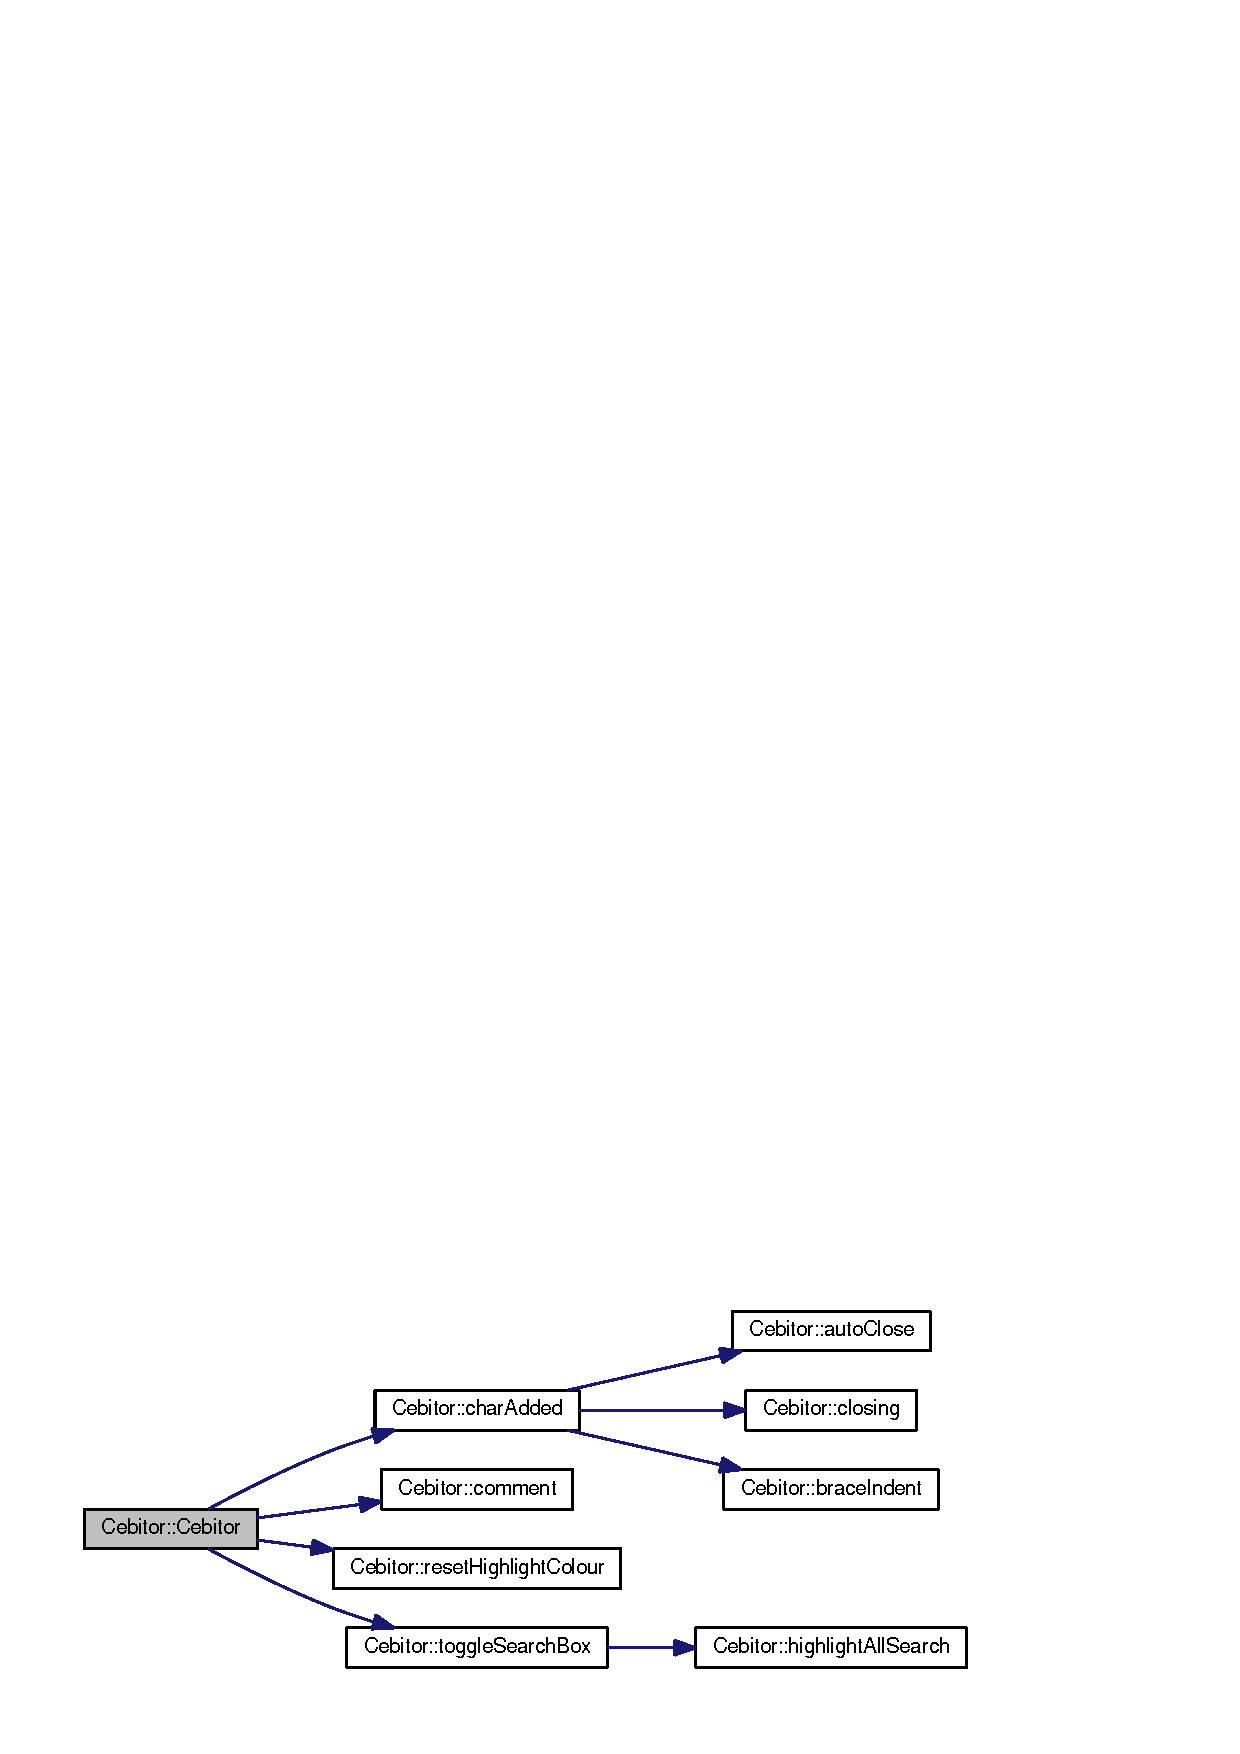
\includegraphics[width=350pt]{class_cebitor_a8295f41644184b799f7c0165627f391a_cgraph}
\end{center}
\end{figure}




\subsection{Member Function Documentation}
\index{Cebitor@{Cebitor}!auto\-Close@{auto\-Close}}
\index{auto\-Close@{auto\-Close}!Cebitor@{Cebitor}}
\subsubsection[{auto\-Close}]{\setlength{\rightskip}{0pt plus 5cm}bool Cebitor\-::auto\-Close (
\begin{DoxyParamCaption}
\item[{const Q\-String}]{\-\_\-close}
\end{DoxyParamCaption}
)\hspace{0.3cm}{\ttfamily [protected]}}\label{class_cebitor_af4b61a42d87ff45b28200523e4b71a65}


adds closing character for braces and quotes 


\begin{DoxyParams}[1]{Parameters}
\mbox{\tt in}  & {\em \-\_\-close} & closing character \\
\hline
\end{DoxyParams}
\begin{DoxyReturn}{Returns}
true if closing character is added 
\end{DoxyReturn}


Definition at line 177 of file Cebitor.\-cpp.


\begin{DoxyCode}
178 \{
179   \textcolor{keywordtype}{int} cursorIndex;
180   \textcolor{keywordtype}{int} cursorLine;
181   \textcolor{keywordtype}{int} length;
182   getCursorPosition(&cursorLine, &cursorIndex);
183   length = lineLength(cursorLine);
184 
185   \textcolor{comment}{// special case for if cursor is on last line since in has no EOL}
186   \textcolor{keywordflow}{if} (cursorLine == lines()-1) \{ length++; \}
187   \textcolor{comment}{// insert closing character if cursor is at EOL or the next character is space}
188   \textcolor{keywordflow}{if}(cursorIndex == length-1 ||
189      text(cursorLine).at(cursorIndex).toLatin1() == \textcolor{charliteral}{' '})
190   \{
191     insert(\_close);
192     \textcolor{keywordflow}{return} \textcolor{keyword}{true};
193   \}
194   \textcolor{keywordflow}{return} \textcolor{keyword}{false};
195 \}
\end{DoxyCode}


Here is the caller graph for this function\-:\nopagebreak
\begin{figure}[H]
\begin{center}
\leavevmode
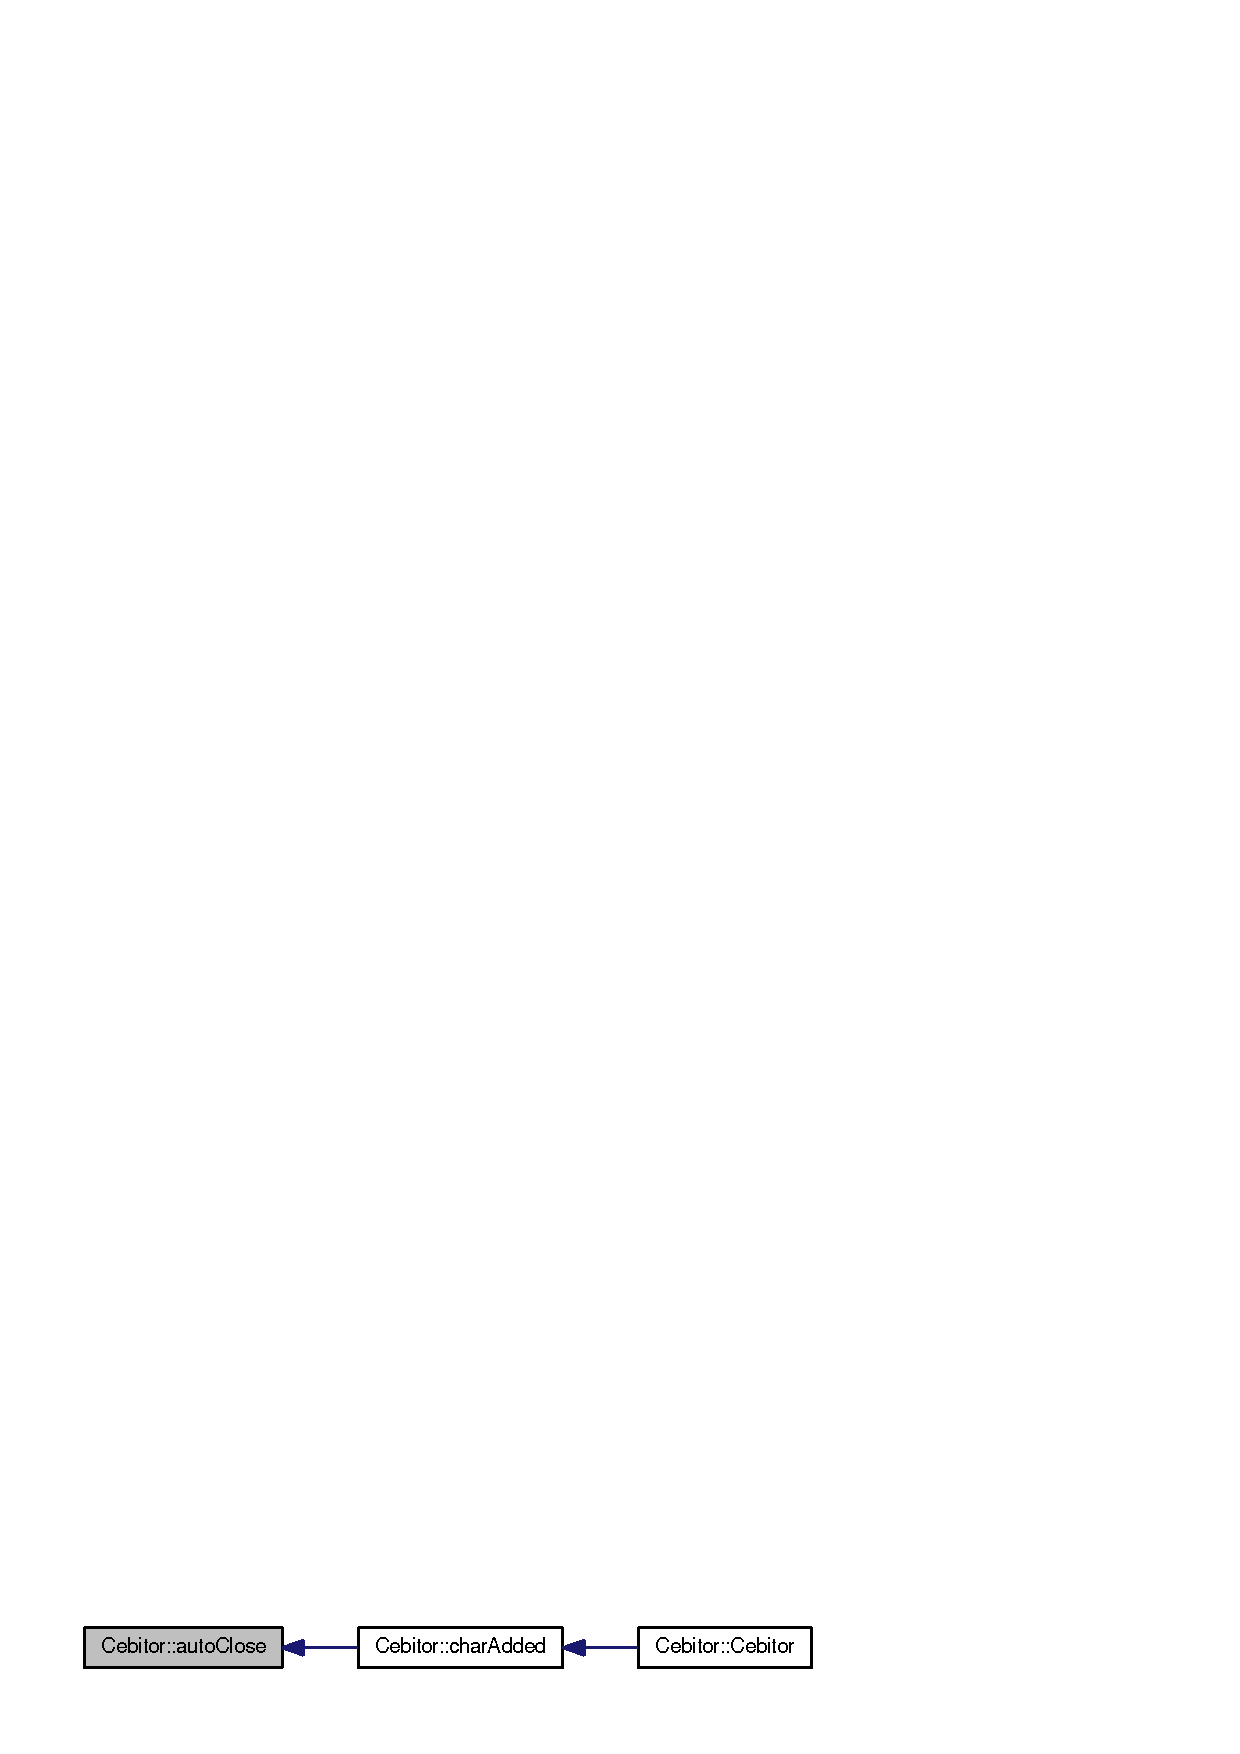
\includegraphics[width=350pt]{class_cebitor_af4b61a42d87ff45b28200523e4b71a65_icgraph}
\end{center}
\end{figure}


\index{Cebitor@{Cebitor}!brace\-Indent@{brace\-Indent}}
\index{brace\-Indent@{brace\-Indent}!Cebitor@{Cebitor}}
\subsubsection[{brace\-Indent}]{\setlength{\rightskip}{0pt plus 5cm}void Cebitor\-::brace\-Indent (
\begin{DoxyParamCaption}
{}
\end{DoxyParamCaption}
)\hspace{0.3cm}{\ttfamily [protected]}}\label{class_cebitor_af923411a34a12c7deb9698a10d5b6c38}


adds indentation after newline following a \char`\"{}\{\char`\"{} 



Definition at line 323 of file Cebitor.\-cpp.


\begin{DoxyCode}
324 \{
325   \textcolor{keywordtype}{int} cursorIndex;
326   \textcolor{keywordtype}{int} cursorLine;
327   QString currentLine;
328   QString previousLine;
329   getCursorPosition(&cursorLine, &cursorIndex);
330   currentLine = text(cursorLine);
331   previousLine = text(cursorLine-1);
332 
333   \textcolor{comment}{// indent if previous line ends with "\{"}
334   \textcolor{keywordflow}{if}(previousLine.endsWith(\textcolor{stringliteral}{"\{\(\backslash\)n"}))
335   \{
336     \textcolor{keywordtype}{int} indentSize;
337     indentSize = indentation(cursorLine-1);
338     setIndentation(cursorLine, indentSize+indentationWidth());
339     cursorIndex = cursorIndex+indentationWidth();
340     setCursorPosition(cursorLine, cursorIndex);
341     currentLine = text(cursorLine);
342     \textcolor{comment}{// extra newline to separate "\{\}"}
343     \textcolor{keywordflow}{if}(currentLine.indexOf(\textcolor{stringliteral}{"\}"}) == cursorIndex)
344     \{
345       insert(QString(\textcolor{stringliteral}{"\(\backslash\)n"}));
346     \}
347   \}
348 
349   \textcolor{comment}{// unindent if "\}" after cursor}
350   \textcolor{keywordflow}{else} \textcolor{keywordflow}{if}(currentLine.indexOf(\textcolor{stringliteral}{"\}"}) == cursorIndex)
351   \{
352     \textcolor{keywordtype}{int} indentSize;
353     indentSize = indentation(cursorLine)-indentationWidth();
354     \textcolor{keywordflow}{if}( indentSize < 0 )
355     \{
356       indentSize = 0;
357     \}
358     setIndentation(cursorLine, indentSize);
359   \}
360 \}
\end{DoxyCode}


Here is the caller graph for this function\-:\nopagebreak
\begin{figure}[H]
\begin{center}
\leavevmode
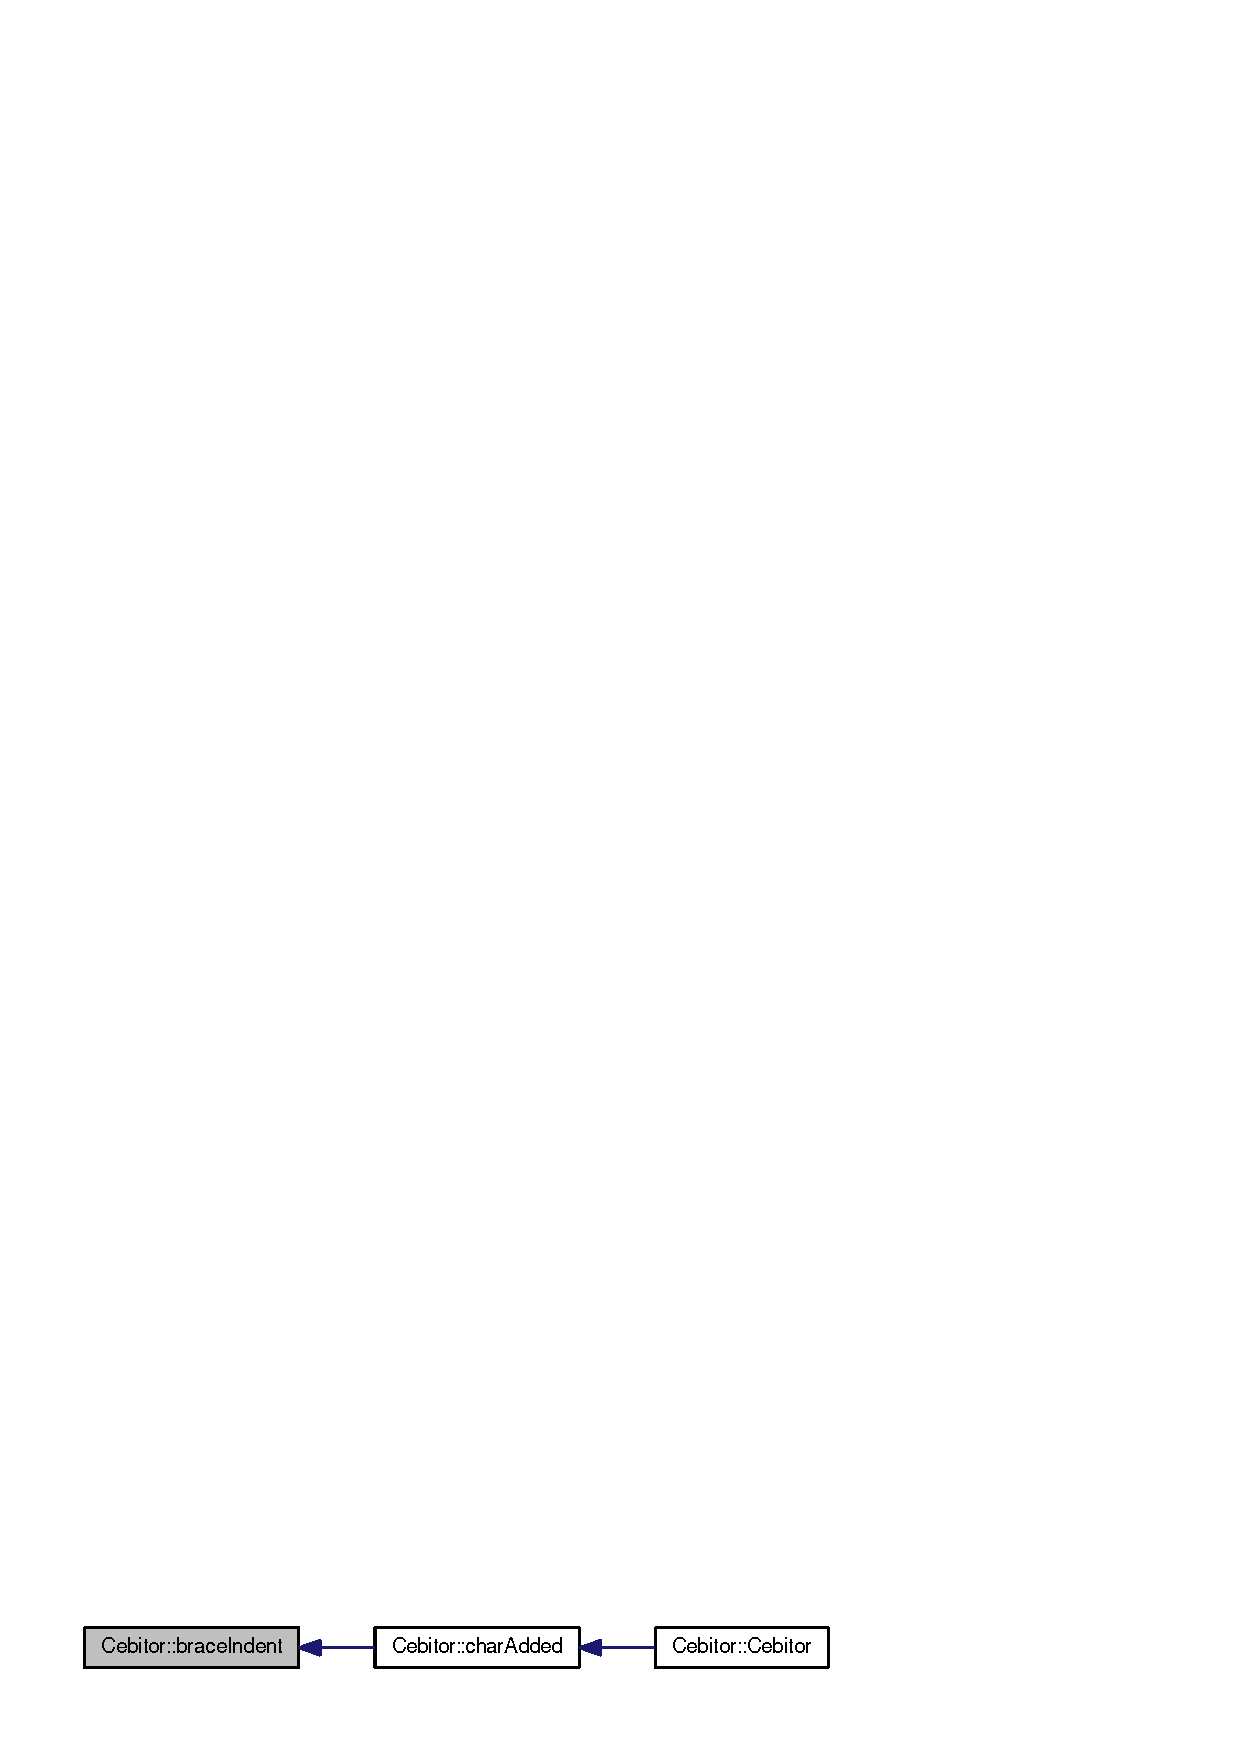
\includegraphics[width=350pt]{class_cebitor_af923411a34a12c7deb9698a10d5b6c38_icgraph}
\end{center}
\end{figure}


\index{Cebitor@{Cebitor}!char\-Added@{char\-Added}}
\index{char\-Added@{char\-Added}!Cebitor@{Cebitor}}
\subsubsection[{char\-Added}]{\setlength{\rightskip}{0pt plus 5cm}void Cebitor\-::char\-Added (
\begin{DoxyParamCaption}
\item[{const int}]{\-\_\-c}
\end{DoxyParamCaption}
)\hspace{0.3cm}{\ttfamily [protected]}, {\ttfamily [slot]}}\label{class_cebitor_a68848533a814f6a1fd5702713a1a2a68}


called when a character is added 



Definition at line 364 of file Cebitor.\-cpp.



References auto\-Close(), brace\-Indent(), and closing().


\begin{DoxyCode}
365 \{
366   \textcolor{keywordflow}{switch}(\_c)
367   \{
368     \textcolor{keywordflow}{case} (\textcolor{keywordtype}{int}) \textcolor{charliteral}{'('}: \{ autoClose(QString(\textcolor{charliteral}{')'})); \textcolor{keywordflow}{break}; \}
369     \textcolor{keywordflow}{case} (\textcolor{keywordtype}{int}) \textcolor{charliteral}{'\{'}: \{ autoClose(QString(\textcolor{charliteral}{'\}'})); \textcolor{keywordflow}{break}; \}
370     \textcolor{keywordflow}{case} (\textcolor{keywordtype}{int}) \textcolor{charliteral}{'['}: \{ autoClose(QString(\textcolor{charliteral}{']'})); \textcolor{keywordflow}{break}; \}
371 
372     \textcolor{keywordflow}{case} (\textcolor{keywordtype}{int}) \textcolor{charliteral}{')'}: \{ closing(QString(\textcolor{charliteral}{')'})); \textcolor{keywordflow}{break}; \}
373     \textcolor{keywordflow}{case} (\textcolor{keywordtype}{int}) \textcolor{charliteral}{'\}'}: \{ closing(QString(\textcolor{charliteral}{'\}'})); \textcolor{keywordflow}{break}; \}
374     \textcolor{keywordflow}{case} (\textcolor{keywordtype}{int}) \textcolor{charliteral}{']'}: \{ closing(QString(\textcolor{charliteral}{']'})); \textcolor{keywordflow}{break}; \}
375 
376     \textcolor{comment}{// special case since " opens and closes}
377     \textcolor{keywordflow}{case} (\textcolor{keywordtype}{int}) \textcolor{charliteral}{'"'}:
378     \{
379       \textcolor{keywordflow}{if}(!closing(QString(\textcolor{charliteral}{'"'})))
380       \{
381         autoClose(QString(\textcolor{charliteral}{'"'}));
382       \}
383       \textcolor{keywordflow}{break};
384     \}
385 
386     \textcolor{comment}{// auto indent for braces}
387     \textcolor{keywordflow}{case} (\textcolor{keywordtype}{int}) \textcolor{charliteral}{'\(\backslash\)n'}: \{ braceIndent(); \textcolor{keywordflow}{break}; \}
388   \}
389 \}
\end{DoxyCode}


Here is the call graph for this function\-:\nopagebreak
\begin{figure}[H]
\begin{center}
\leavevmode
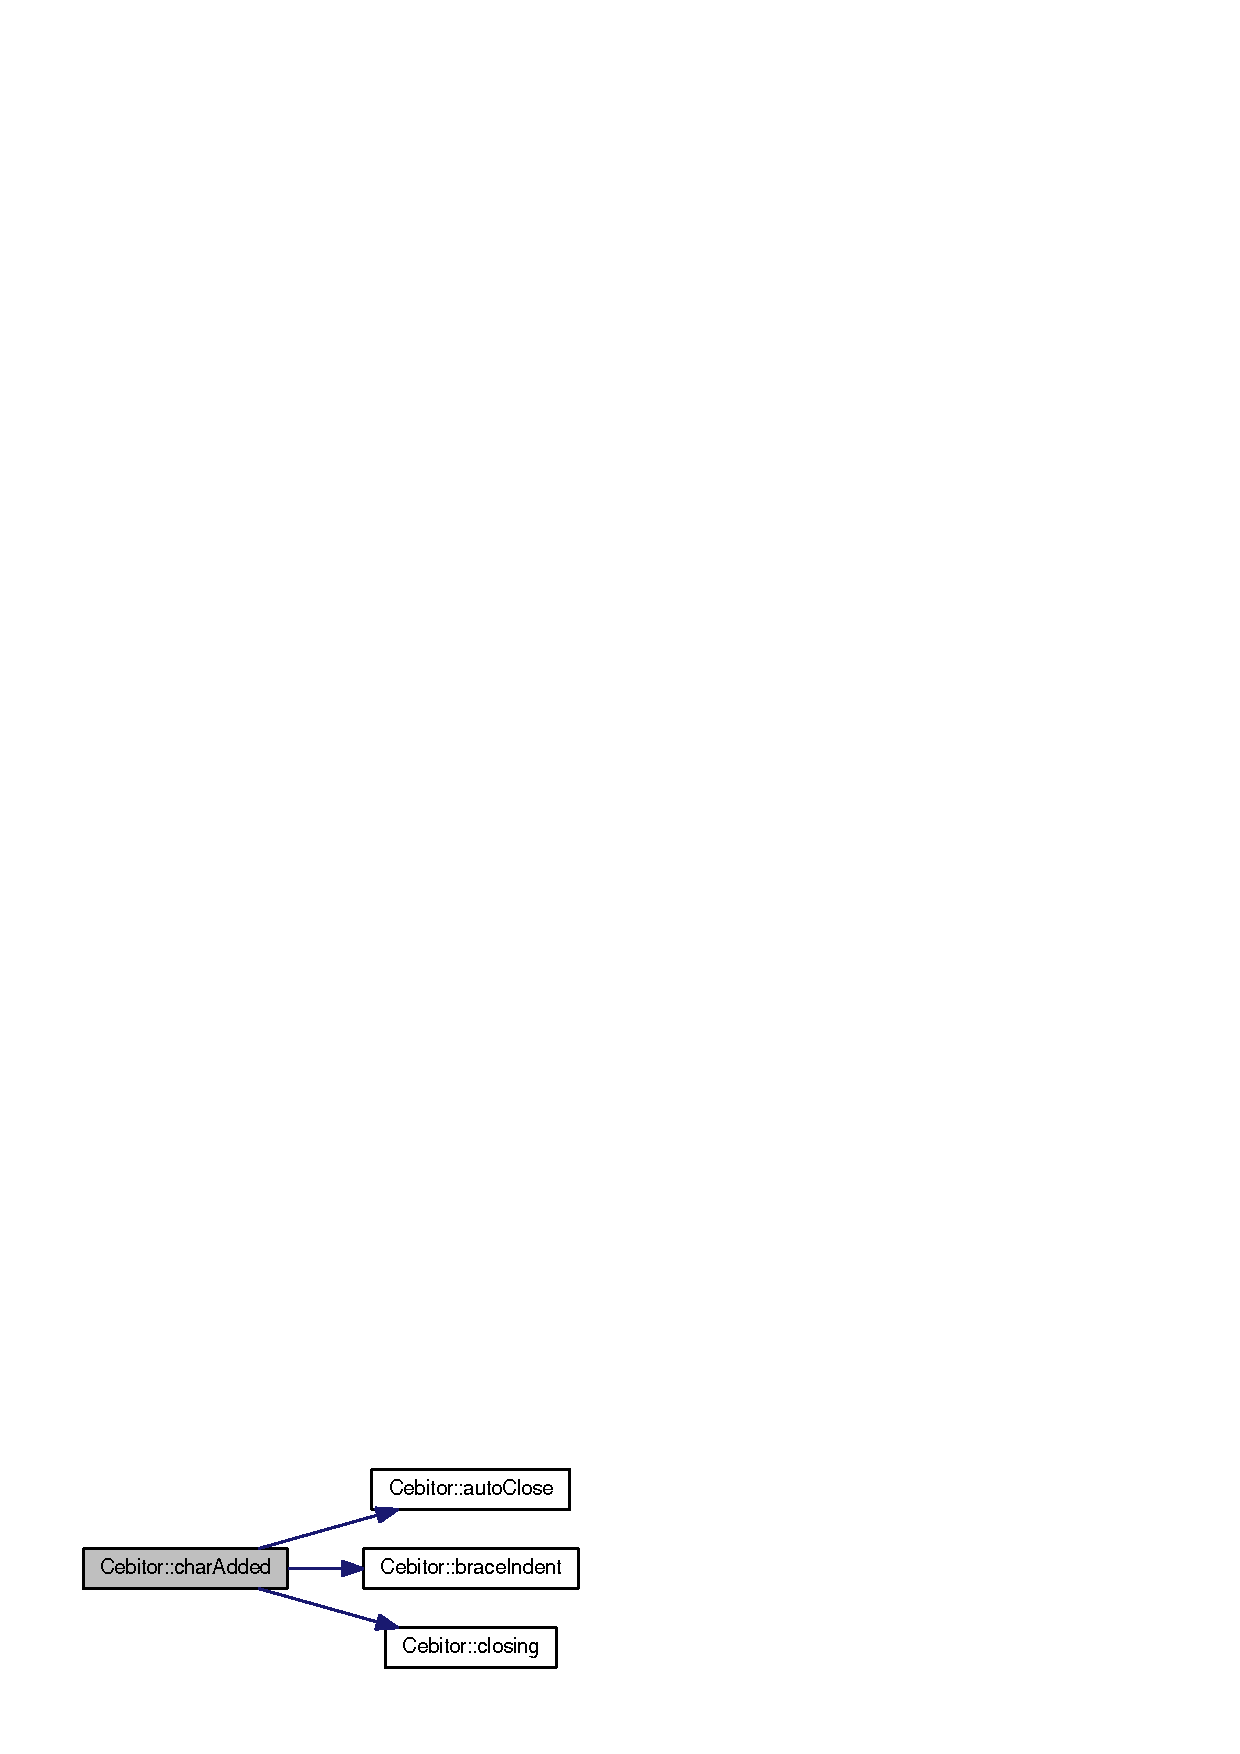
\includegraphics[width=282pt]{class_cebitor_a68848533a814f6a1fd5702713a1a2a68_cgraph}
\end{center}
\end{figure}




Here is the caller graph for this function\-:\nopagebreak
\begin{figure}[H]
\begin{center}
\leavevmode
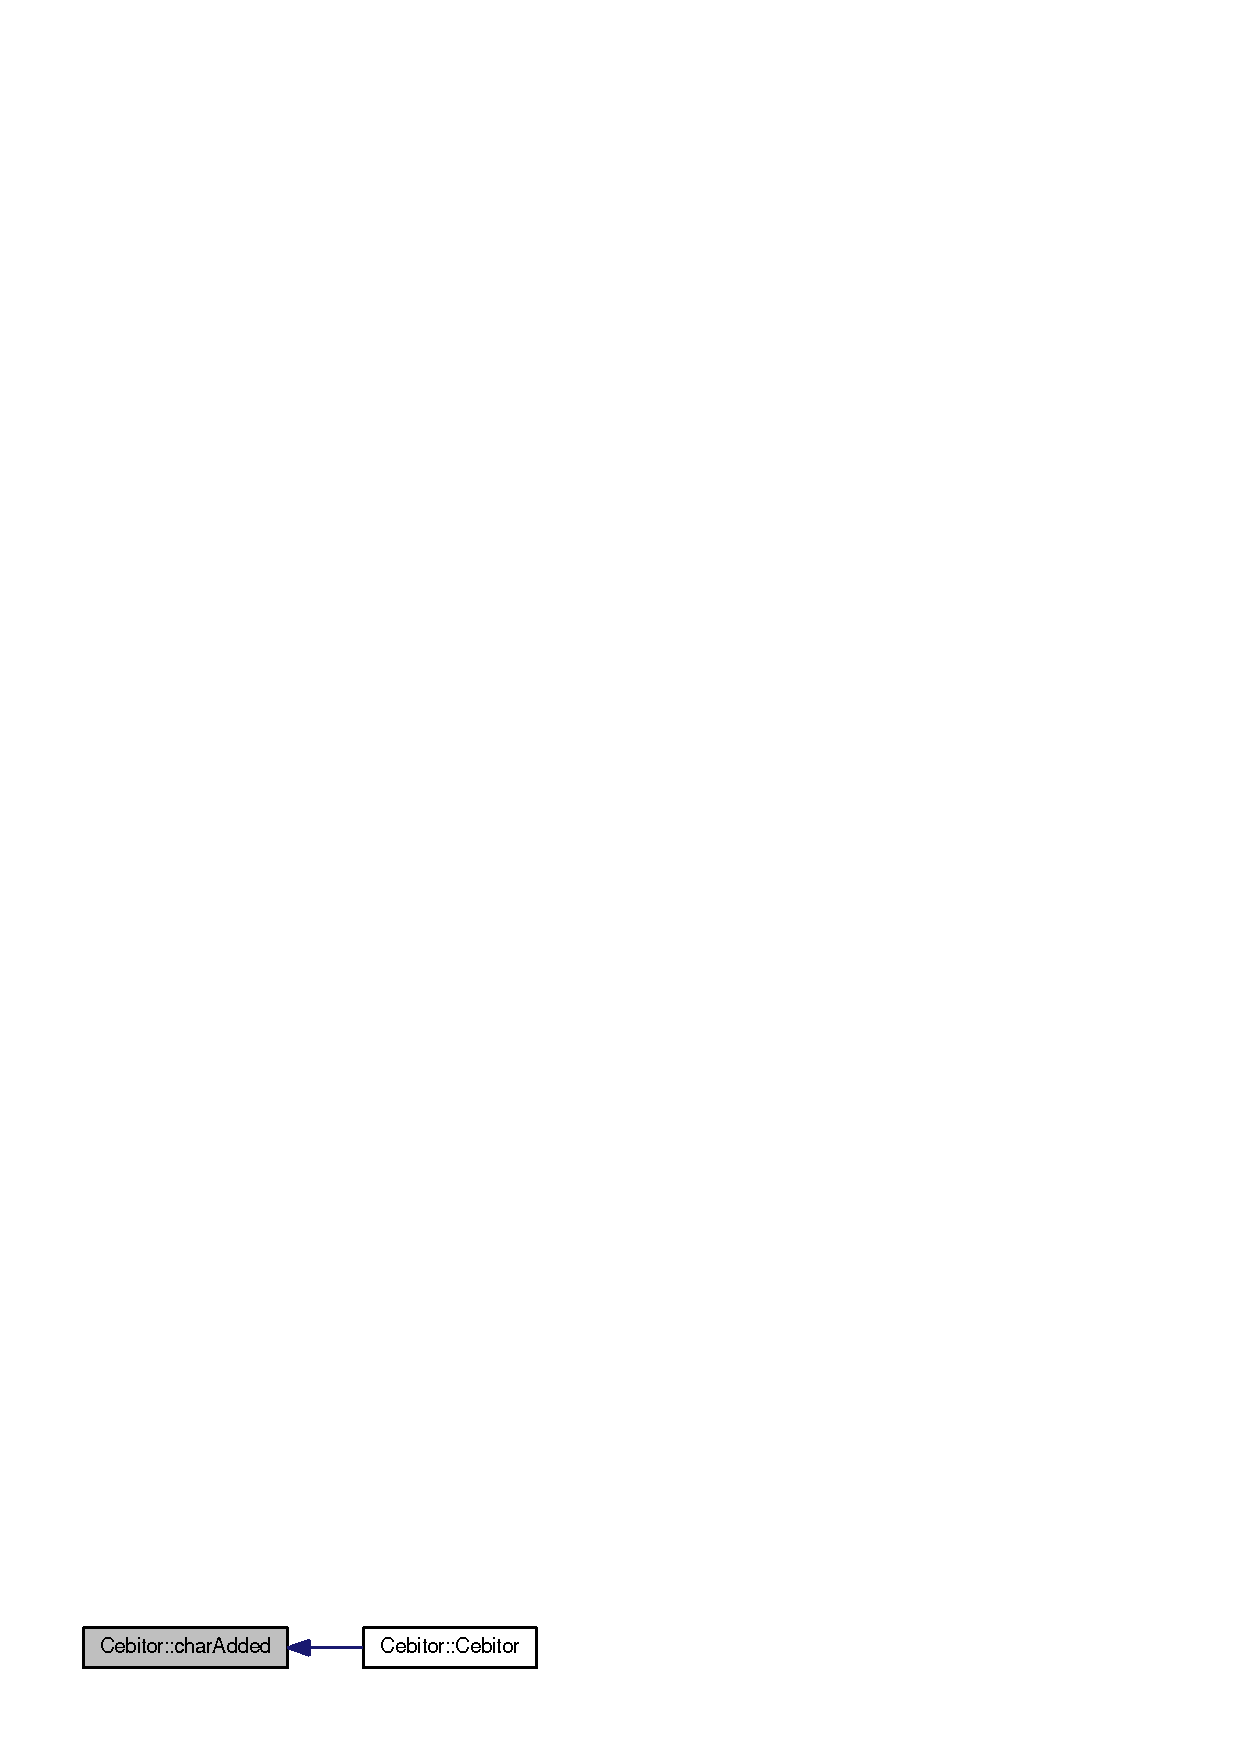
\includegraphics[width=262pt]{class_cebitor_a68848533a814f6a1fd5702713a1a2a68_icgraph}
\end{center}
\end{figure}


\index{Cebitor@{Cebitor}!clear\-Errors@{clear\-Errors}}
\index{clear\-Errors@{clear\-Errors}!Cebitor@{Cebitor}}
\subsubsection[{clear\-Errors}]{\setlength{\rightskip}{0pt plus 5cm}void Cebitor\-::clear\-Errors (
\begin{DoxyParamCaption}
{}
\end{DoxyParamCaption}
)\hspace{0.3cm}{\ttfamily [slot]}}\label{class_cebitor_aef8e5eebfe92c418aacd15fc83f8799b}


Removes all error and warning line markers. 



Definition at line 104 of file Cebitor.\-cpp.


\begin{DoxyCode}
105 \{
106   markerDeleteAll(MarkerType::ERROR);
107   markerDeleteAll(MarkerType::WARNING);
108 \}
\end{DoxyCode}
\index{Cebitor@{Cebitor}!closing@{closing}}
\index{closing@{closing}!Cebitor@{Cebitor}}
\subsubsection[{closing}]{\setlength{\rightskip}{0pt plus 5cm}bool Cebitor\-::closing (
\begin{DoxyParamCaption}
\item[{const Q\-String}]{\-\_\-close}
\end{DoxyParamCaption}
)\hspace{0.3cm}{\ttfamily [protected]}}\label{class_cebitor_a759c7d4cb58cc46c43e203f26320a2aa}


removes duplicates of closing braces and quotes 


\begin{DoxyParams}[1]{Parameters}
\mbox{\tt in}  & {\em \-\_\-close} & closing character \\
\hline
\end{DoxyParams}
\begin{DoxyReturn}{Returns}
true if duplicate character is replaced 
\end{DoxyReturn}


Definition at line 199 of file Cebitor.\-cpp.


\begin{DoxyCode}
200 \{
201   \textcolor{keywordtype}{int} cursorIndex;
202   \textcolor{keywordtype}{int} cursorLine;
203   getCursorPosition(&cursorLine, &cursorIndex);
204 
205   \textcolor{keywordtype}{int} length = lineLength(cursorLine);
206 
207   \textcolor{comment}{// special case for if cursor is last position in file}
208   \textcolor{keywordflow}{if}(cursorLine == lines()-1 && length == cursorIndex)
209   \{
210     \textcolor{keywordflow}{return} \textcolor{keyword}{false};
211   \}
212   \textcolor{comment}{// remove duplicate if next character is the same as \_close}
213   \textcolor{keywordflow}{if}(text(cursorLine).at(cursorIndex) == \_close.at(0))
214   \{
215     setSelection(cursorLine, cursorIndex, cursorLine, cursorIndex+1);
216     removeSelectedText();
217     \textcolor{keywordflow}{return} \textcolor{keyword}{true};
218   \}
219   \textcolor{comment}{// auto unindent "\}"}
220   \textcolor{keywordflow}{if}( \_close == QString(\textcolor{charliteral}{'\}'}) && cursorIndex == indentation(cursorLine)+1 )
221   \{
222     \textcolor{keywordtype}{int} indentSize;
223     indentSize = indentation(cursorLine)-indentationWidth();
224     \textcolor{keywordflow}{if}( indentSize < 0 )
225     \{
226       indentSize = 0;
227     \}
228     setIndentation(cursorLine, indentSize);
229   \}
230   \textcolor{keywordflow}{return} \textcolor{keyword}{false};
231 \}
\end{DoxyCode}


Here is the caller graph for this function\-:\nopagebreak
\begin{figure}[H]
\begin{center}
\leavevmode
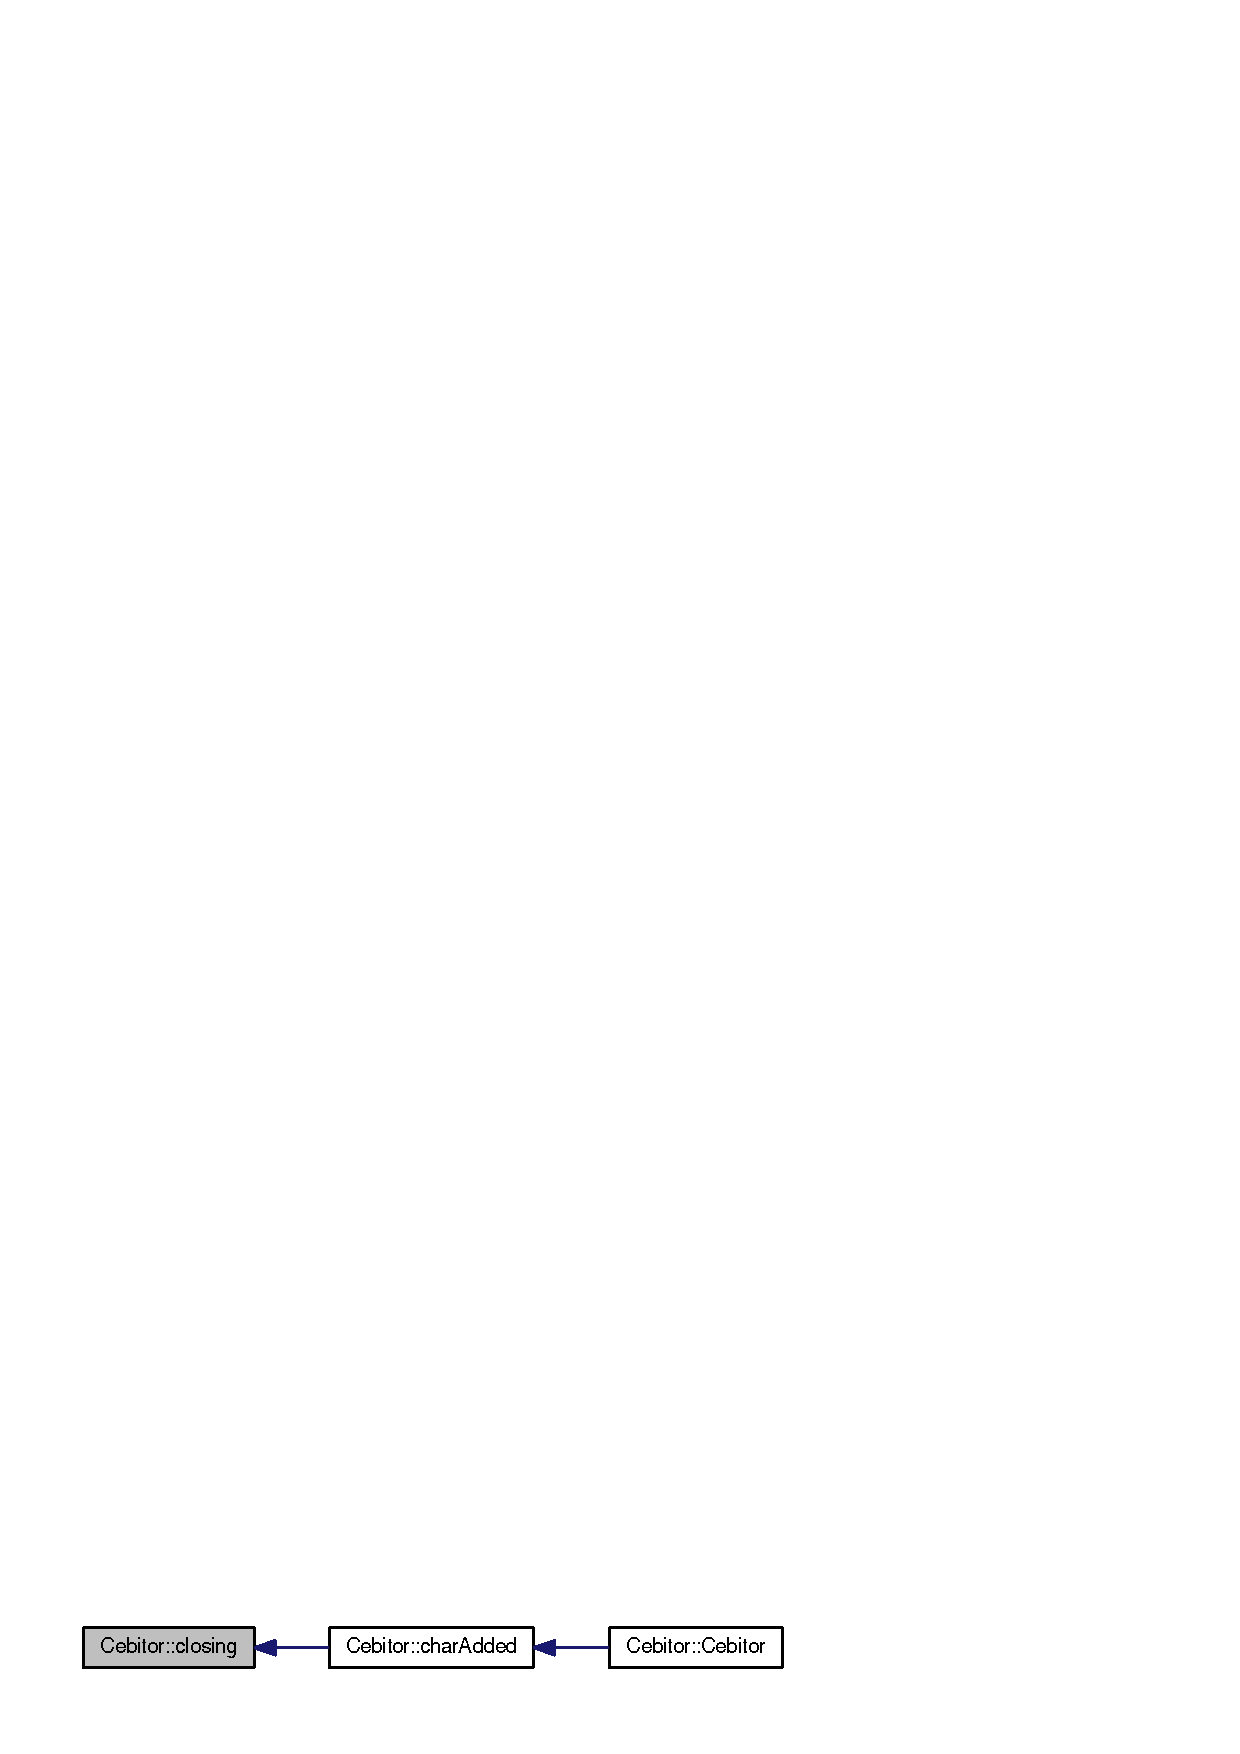
\includegraphics[width=350pt]{class_cebitor_a759c7d4cb58cc46c43e203f26320a2aa_icgraph}
\end{center}
\end{figure}


\index{Cebitor@{Cebitor}!comment@{comment}}
\index{comment@{comment}!Cebitor@{Cebitor}}
\subsubsection[{comment}]{\setlength{\rightskip}{0pt plus 5cm}void Cebitor\-::comment (
\begin{DoxyParamCaption}
{}
\end{DoxyParamCaption}
)\hspace{0.3cm}{\ttfamily [protected]}, {\ttfamily [slot]}}\label{class_cebitor_a024169eef080f400c6c9384d8229f983}


comment out all selected lines 



Definition at line 235 of file Cebitor.\-cpp.


\begin{DoxyCode}
236 \{
237   beginUndoAction();
238   \textcolor{keywordtype}{int} lineFrom;
239   \textcolor{keywordtype}{int} indexFrom;
240   \textcolor{keywordtype}{int} lineTo;
241   \textcolor{keywordtype}{int} indexTo;
242   \textcolor{comment}{// get selected lines or current line if no text is selected}
243   \textcolor{keywordflow}{if}(hasSelectedText())
244   \{
245     getSelection(&lineFrom, &indexFrom, &lineTo, &indexTo);
246   \}
247   \textcolor{keywordflow}{else}
248   \{
249     getCursorPosition(&lineFrom, &indexFrom);
250     lineTo = lineFrom;
251     indexTo = indexFrom;
252   \}
253 
254   \textcolor{comment}{// check if selected lines are already commented}
255   \textcolor{keywordtype}{bool} alreadyCommented = \textcolor{keyword}{true};
256   \textcolor{keywordflow}{for}(\textcolor{keywordtype}{int} i=lineFrom; i<=lineTo; i++)
257   \{
258     QString lineText = text(i);
259     \textcolor{keywordflow}{if}(!lineText.startsWith(\textcolor{stringliteral}{"//"}))
260     \{
261       alreadyCommented = \textcolor{keyword}{false};
262     \}
263   \}
264 
265   \textcolor{comment}{// remove "//" from each line if they are already commented}
266   \textcolor{keywordflow}{if}(alreadyCommented)
267   \{
268     \textcolor{keywordflow}{for}(\textcolor{keywordtype}{int} i=lineFrom; i<=lineTo; i++)
269     \{
270       setSelection(i,0,i,2);
271       removeSelectedText();
272     \}
273     \textcolor{comment}{//offset original selection for reselecting text}
274     indexTo -= 2;
275     \textcolor{keywordflow}{if}(indexFrom > 1)
276     \{
277       indexFrom -= 2;
278     \}
279   \}
280 
281   \textcolor{comment}{// insert "//" at the start of each line}
282   \textcolor{keywordflow}{else}
283   \{
284     \textcolor{keywordflow}{for}(\textcolor{keywordtype}{int} i=lineFrom; i<=lineTo; i++)
285     \{
286       insertAt(QString(\textcolor{stringliteral}{"//"}),i,0);
287     \}
288     \textcolor{comment}{//offset original selection for reselecting text}
289     indexTo += 2;
290     \textcolor{keywordflow}{if}(indexFrom != 0)
291     \{
292       indexFrom += 2;
293     \}
294   \}
295 
296   \textcolor{comment}{// reselect to match original selection}
297   setSelection(lineFrom,indexFrom,lineTo,indexTo);
298   endUndoAction();
299 \}
\end{DoxyCode}


Here is the caller graph for this function\-:\nopagebreak
\begin{figure}[H]
\begin{center}
\leavevmode
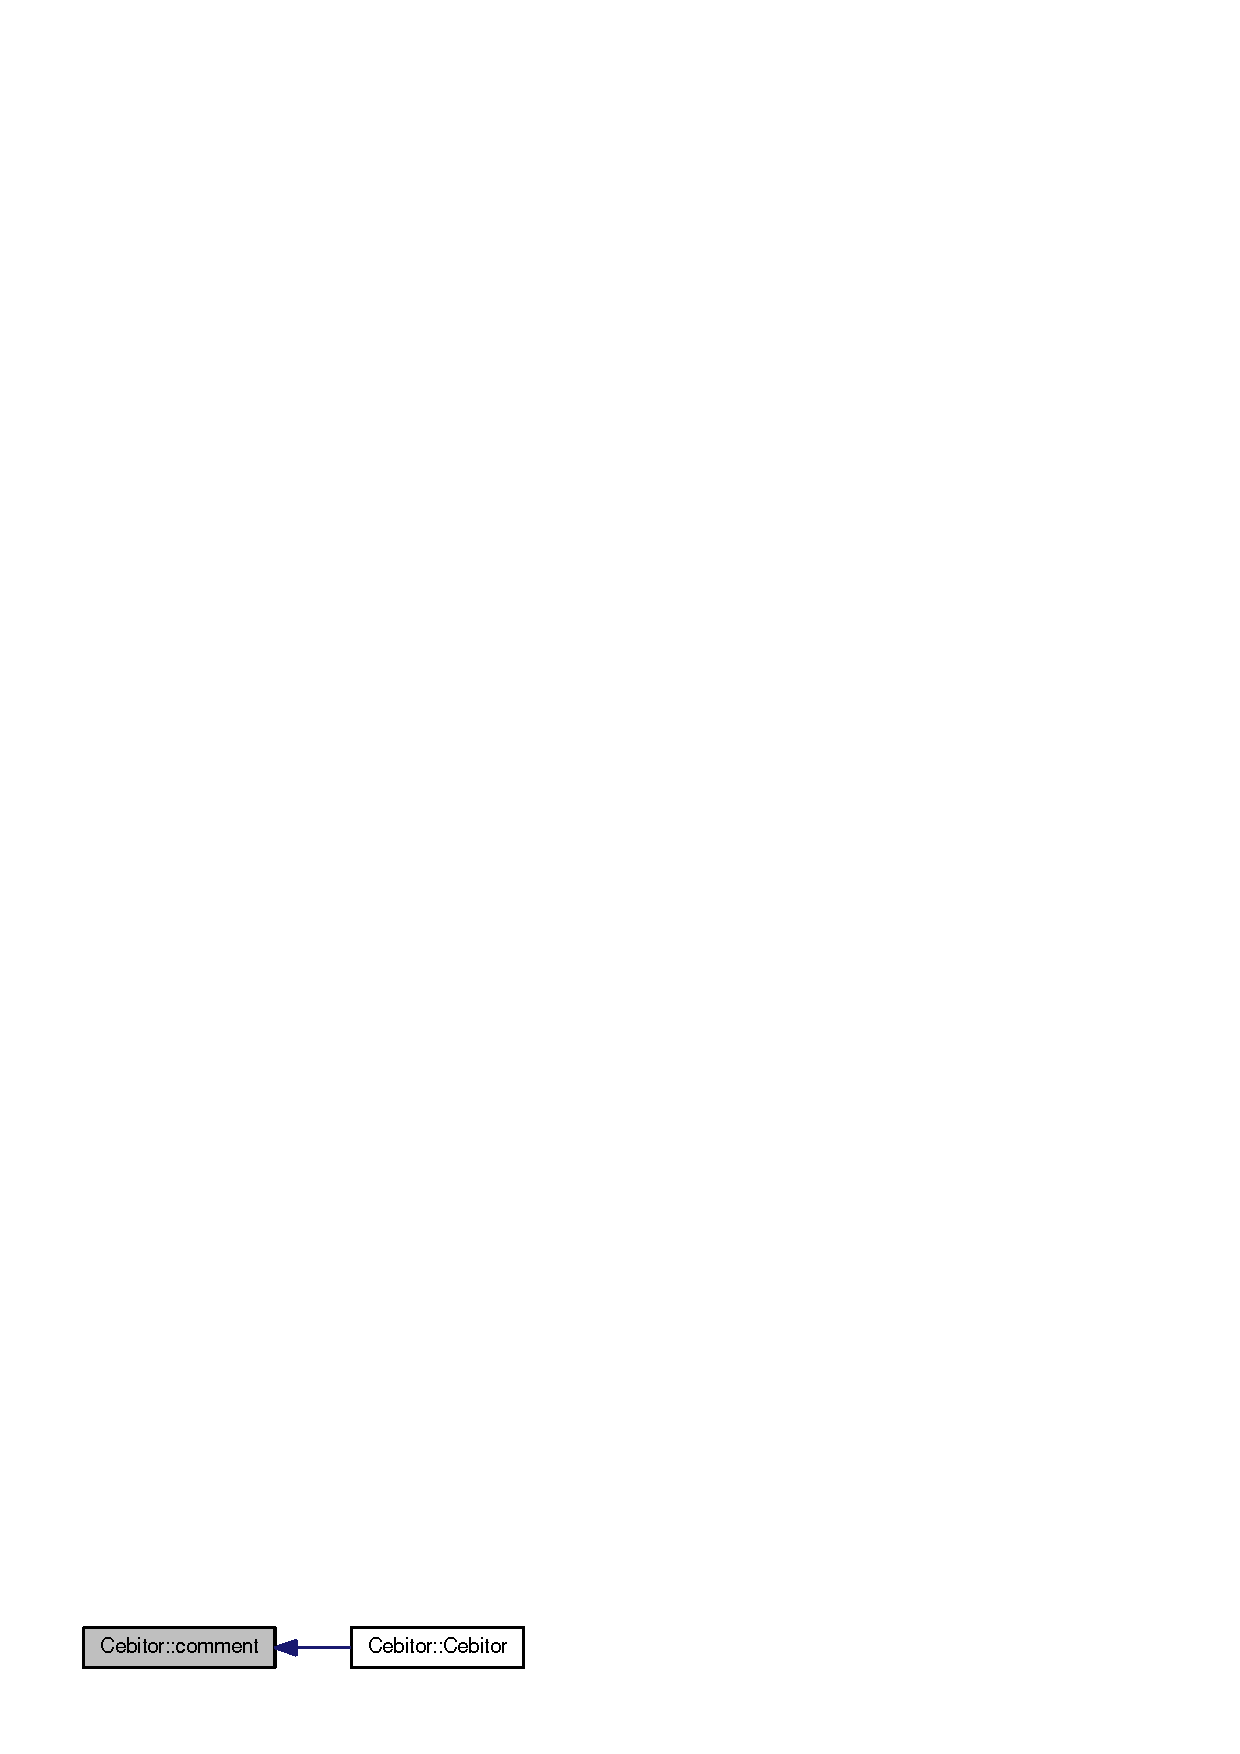
\includegraphics[width=256pt]{class_cebitor_a024169eef080f400c6c9384d8229f983_icgraph}
\end{center}
\end{figure}


\index{Cebitor@{Cebitor}!highlight\-All\-Search@{highlight\-All\-Search}}
\index{highlight\-All\-Search@{highlight\-All\-Search}!Cebitor@{Cebitor}}
\subsubsection[{highlight\-All\-Search}]{\setlength{\rightskip}{0pt plus 5cm}void Cebitor\-::highlight\-All\-Search (
\begin{DoxyParamCaption}
{}
\end{DoxyParamCaption}
)\hspace{0.3cm}{\ttfamily [slot]}}\label{class_cebitor_a1ba2c5c83f98d668f130caeaabac4b63}


sets indicator for each search result 



Definition at line 146 of file Cebitor.\-cpp.



References m\-\_\-search\-Indicator, and m\-\_\-search\-Line\-Edit.


\begin{DoxyCode}
147 \{
148   clearIndicatorRange(0,0,lines(),text(lines()).length(),m_searchIndicator);
149   \textcolor{keywordtype}{int} line;
150   \textcolor{keywordtype}{int} indexFrom;
151   \textcolor{keywordtype}{int} indexTo;
152   QString searchTerm = m_searchLineEdit->text();
153   \textcolor{keywordflow}{if}(searchTerm.length()==0)
154   \{
155     \textcolor{keywordflow}{return};
156   \}
157   \textcolor{keywordtype}{int} current;
158   current = text().indexOf(
159         searchTerm,
160         0,
161         Qt::CaseSensitivity::CaseInsensitive
162         );
163   \textcolor{keywordflow}{while}(current!= -1)
164   \{
165     lineIndexFromPosition(current,&line,&indexFrom);
166     indexTo = indexFrom + searchTerm.length();
167     fillIndicatorRange(line,indexFrom,line,indexTo,m_searchIndicator);
168     current = text().indexOf(searchTerm,
169                              current+1,
170                              Qt::CaseSensitivity::CaseInsensitive
171                              );
172   \}
173 \}
\end{DoxyCode}


Here is the caller graph for this function\-:\nopagebreak
\begin{figure}[H]
\begin{center}
\leavevmode
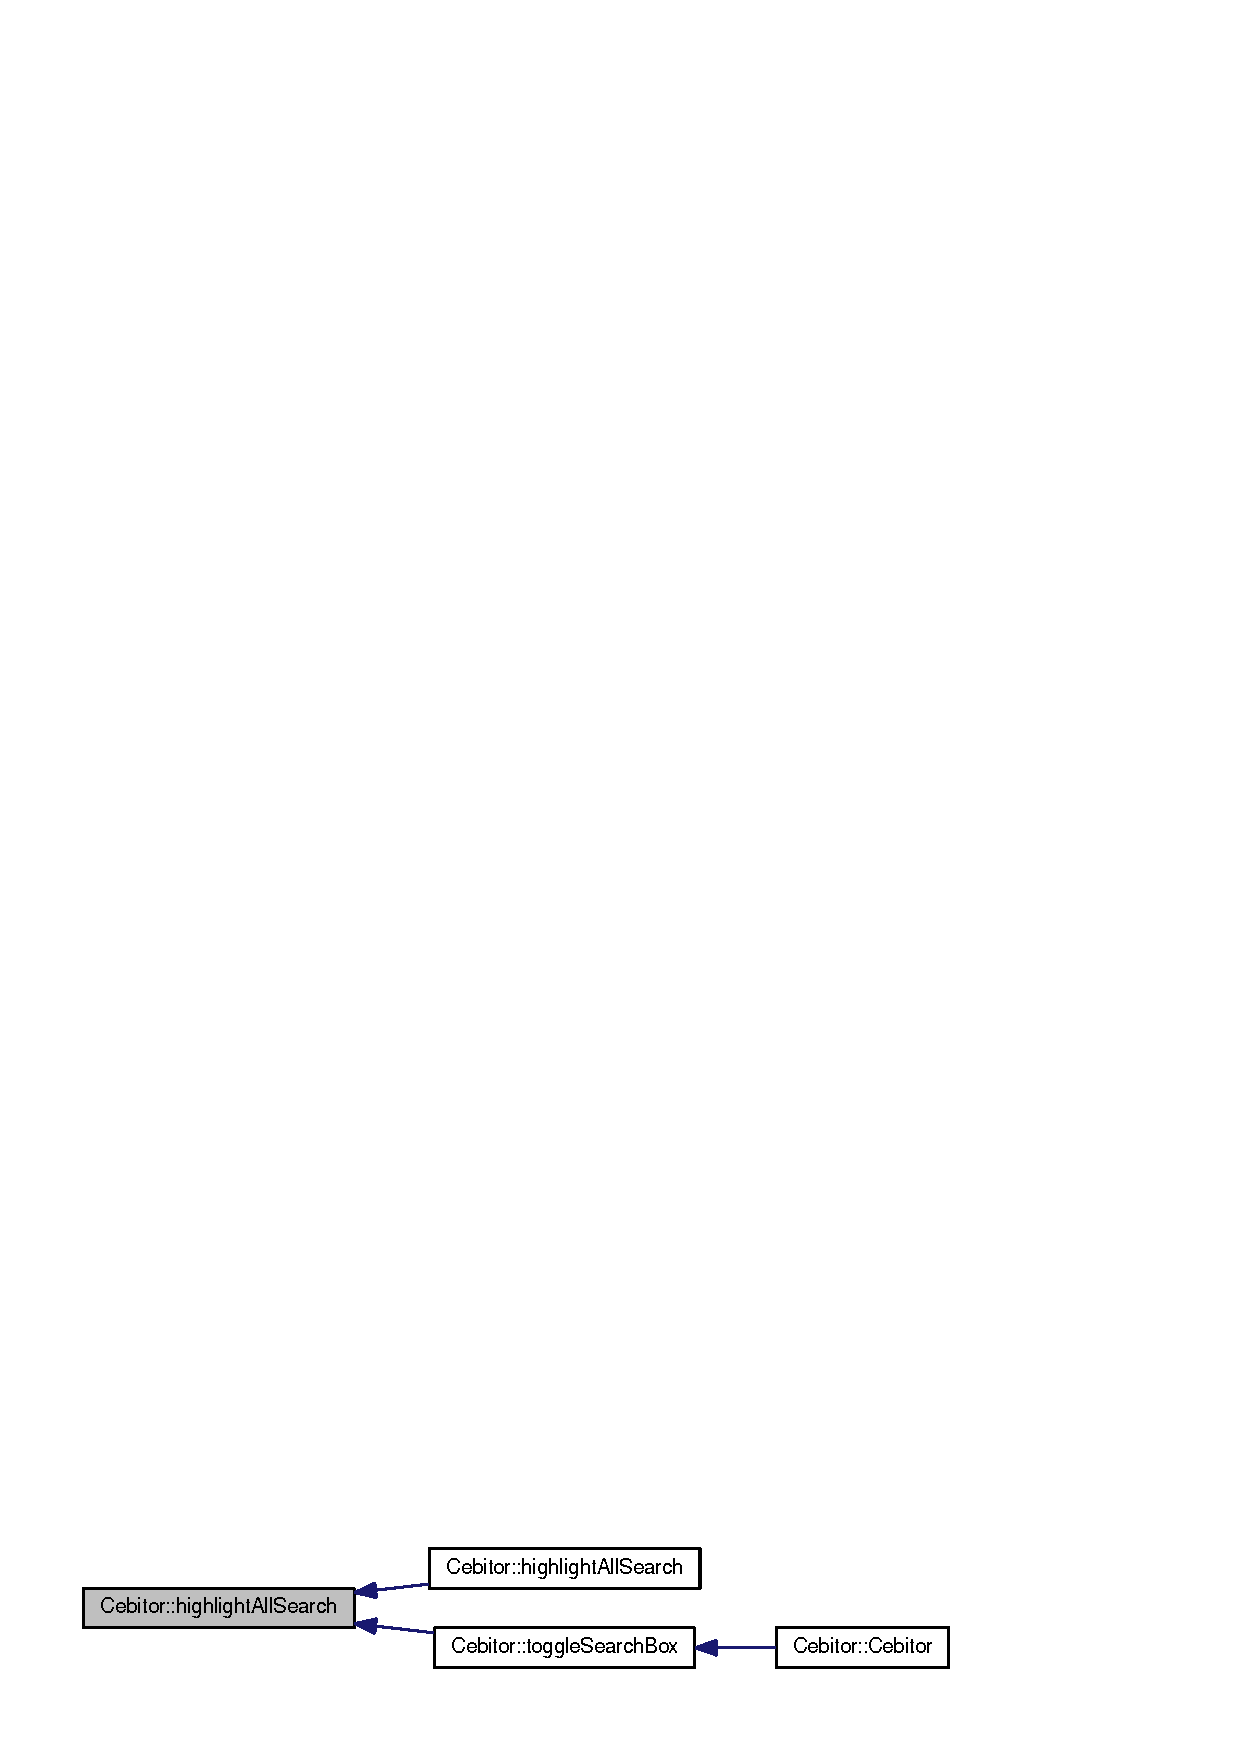
\includegraphics[width=350pt]{class_cebitor_a1ba2c5c83f98d668f130caeaabac4b63_icgraph}
\end{center}
\end{figure}


\index{Cebitor@{Cebitor}!highlight\-All\-Search@{highlight\-All\-Search}}
\index{highlight\-All\-Search@{highlight\-All\-Search}!Cebitor@{Cebitor}}
\subsubsection[{highlight\-All\-Search}]{\setlength{\rightskip}{0pt plus 5cm}void Cebitor\-::highlight\-All\-Search (
\begin{DoxyParamCaption}
\item[{const Q\-String \&}]{\-\_\-text}
\end{DoxyParamCaption}
)\hspace{0.3cm}{\ttfamily [slot]}}\label{class_cebitor_a8eef8da0f000bcfa07ea7b7b780e970d}


sets indicator for each search result 


\begin{DoxyParams}[1]{Parameters}
\mbox{\tt in}  & {\em \-\_\-text} & the text that has been changed \\
\hline
\end{DoxyParams}


Definition at line 140 of file Cebitor.\-cpp.



References highlight\-All\-Search().


\begin{DoxyCode}
141 \{
142   highlightAllSearch();
143 \}
\end{DoxyCode}


Here is the call graph for this function\-:\nopagebreak
\begin{figure}[H]
\begin{center}
\leavevmode
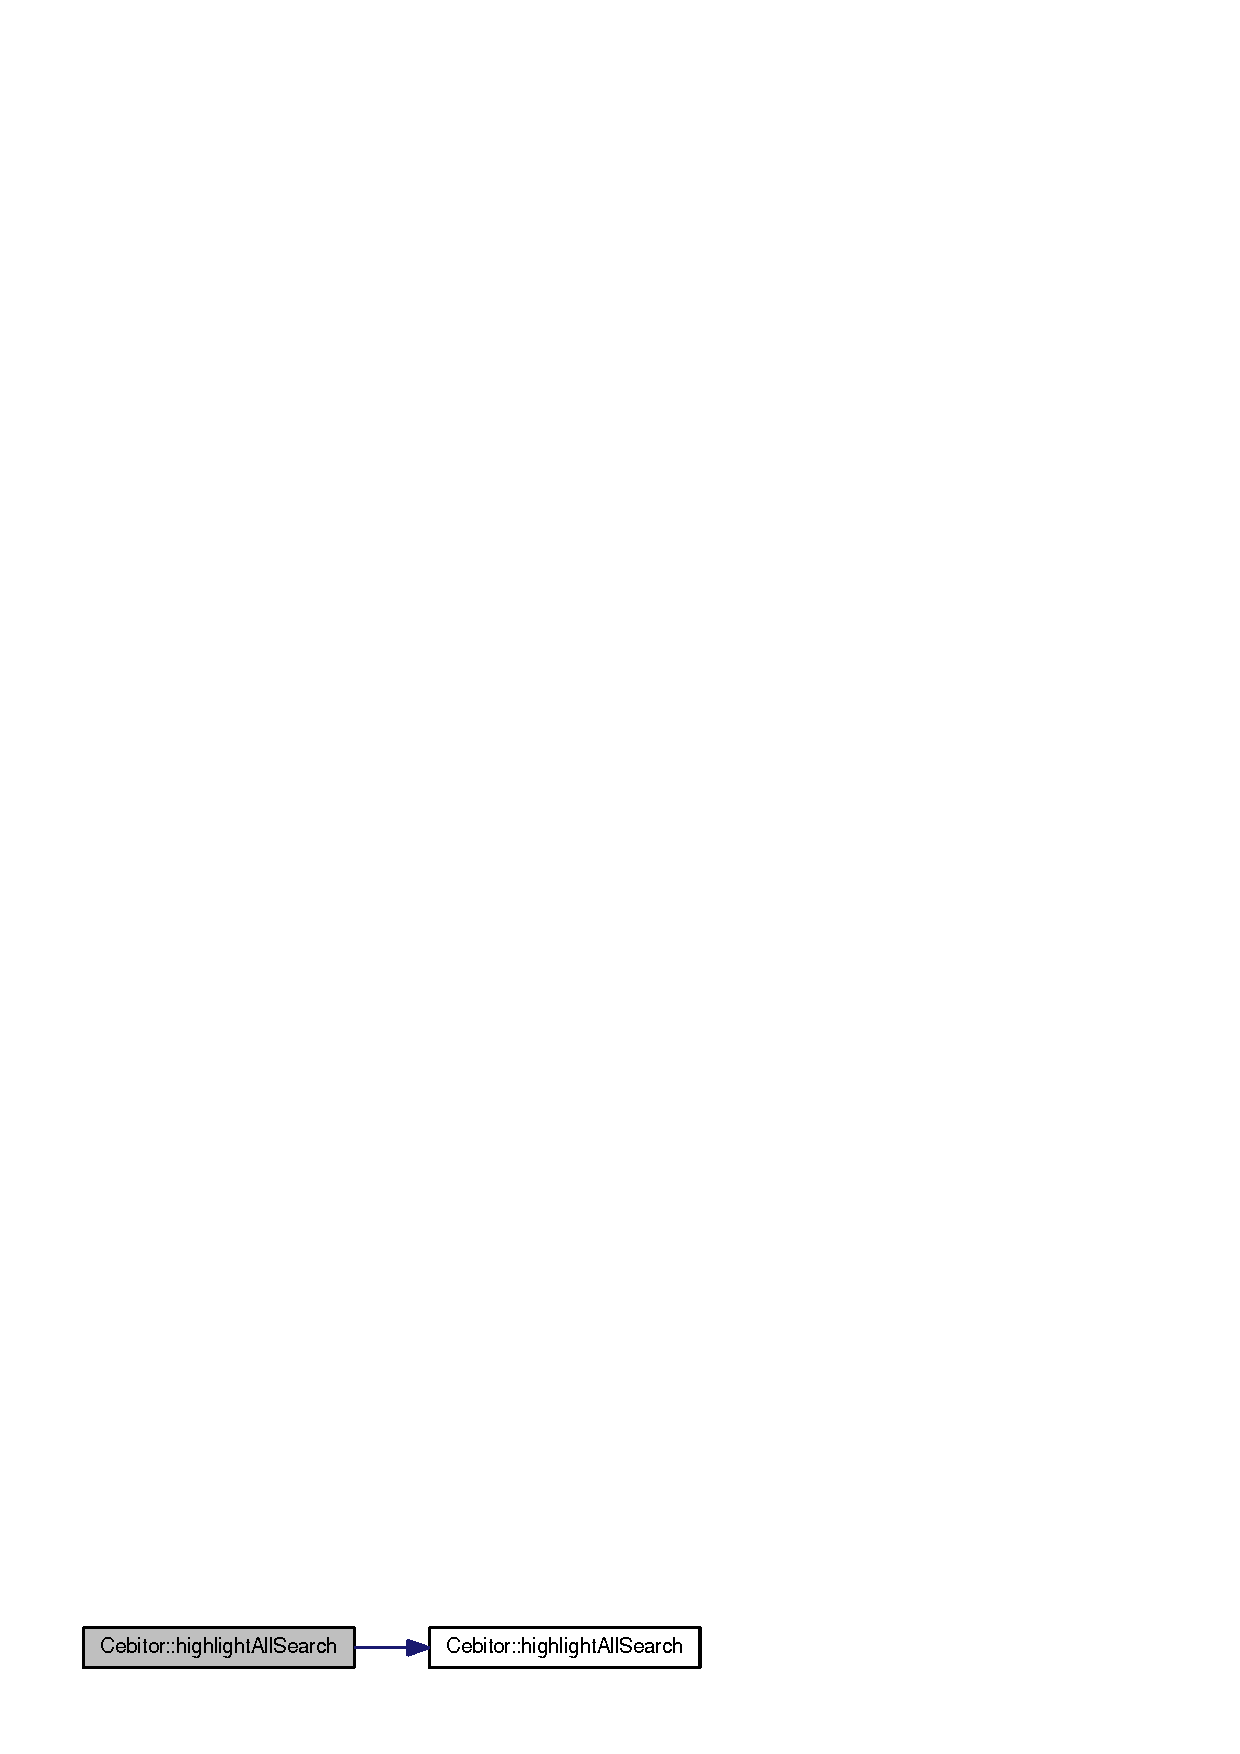
\includegraphics[width=340pt]{class_cebitor_a8eef8da0f000bcfa07ea7b7b780e970d_cgraph}
\end{center}
\end{figure}


\index{Cebitor@{Cebitor}!reset\-Highlight\-Colour@{reset\-Highlight\-Colour}}
\index{reset\-Highlight\-Colour@{reset\-Highlight\-Colour}!Cebitor@{Cebitor}}
\subsubsection[{reset\-Highlight\-Colour}]{\setlength{\rightskip}{0pt plus 5cm}void Cebitor\-::reset\-Highlight\-Colour (
\begin{DoxyParamCaption}
{}
\end{DoxyParamCaption}
)\hspace{0.3cm}{\ttfamily [protected]}, {\ttfamily [slot]}}\label{class_cebitor_a0e98f0691da34de6b4ab1c14d9eea63d}


reset the highlighting colour 



Definition at line 393 of file Cebitor.\-cpp.


\begin{DoxyCode}
394 \{
395   setSelectionBackgroundColor(QColor(61,61,52));
396   resetSelectionForegroundColor();
397 \}
\end{DoxyCode}


Here is the caller graph for this function\-:\nopagebreak
\begin{figure}[H]
\begin{center}
\leavevmode
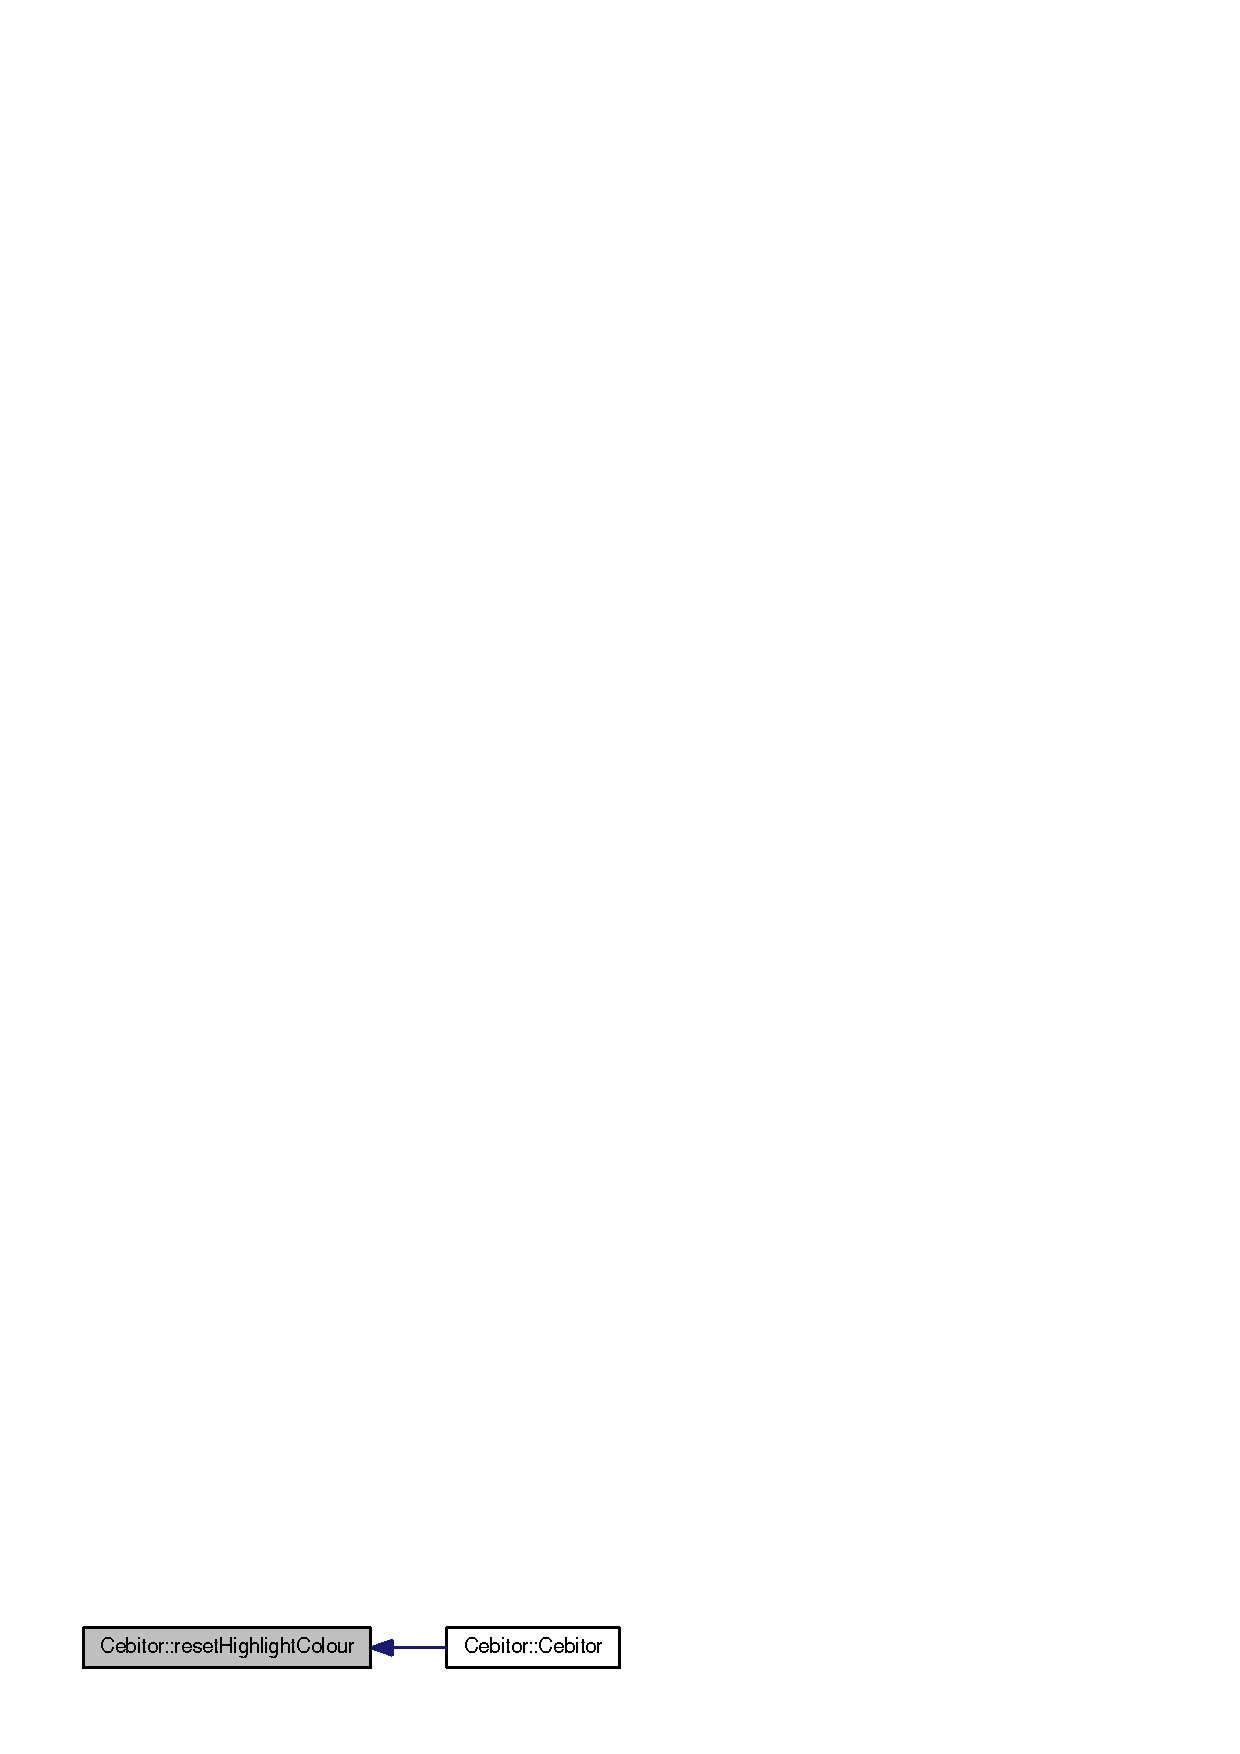
\includegraphics[width=302pt]{class_cebitor_a0e98f0691da34de6b4ab1c14d9eea63d_icgraph}
\end{center}
\end{figure}


\index{Cebitor@{Cebitor}!search\-Next@{search\-Next}}
\index{search\-Next@{search\-Next}!Cebitor@{Cebitor}}
\subsubsection[{search\-Next}]{\setlength{\rightskip}{0pt plus 5cm}void Cebitor\-::search\-Next (
\begin{DoxyParamCaption}
{}
\end{DoxyParamCaption}
)\hspace{0.3cm}{\ttfamily [slot]}}\label{class_cebitor_af195ffc78cfe979bcc72ad93f9236a6c}


Search for next occurance. 



Definition at line 110 of file Cebitor.\-cpp.



References m\-\_\-search\-Line\-Edit.


\begin{DoxyCode}
111 \{
112   QString searchTerm = m_searchLineEdit->text();
113   \textcolor{keywordtype}{bool} found;
114   found = findFirst(searchTerm, \textcolor{keyword}{false}, \textcolor{keyword}{false}, \textcolor{keyword}{false}, \textcolor{keyword}{true});
115   \textcolor{keywordflow}{if}(found)
116   \{
117     setSelectionBackgroundColor(QColor(230, 219, 116));
118     setSelectionForegroundColor(QColor(39,40,34));
119   \}
120 \}
\end{DoxyCode}
\index{Cebitor@{Cebitor}!search\-Prev@{search\-Prev}}
\index{search\-Prev@{search\-Prev}!Cebitor@{Cebitor}}
\subsubsection[{search\-Prev}]{\setlength{\rightskip}{0pt plus 5cm}void Cebitor\-::search\-Prev (
\begin{DoxyParamCaption}
{}
\end{DoxyParamCaption}
)\hspace{0.3cm}{\ttfamily [slot]}}\label{class_cebitor_a54eb5c2c26fbecf66ad80f95cdbb32c7}


Search for previous occurance. 



Definition at line 124 of file Cebitor.\-cpp.



References m\-\_\-search\-Line\-Edit.


\begin{DoxyCode}
125 \{
126   QString searchTerm = m_searchLineEdit->text();
127   \textcolor{keywordtype}{bool} found;
128   found = findFirst(searchTerm, \textcolor{keyword}{false}, \textcolor{keyword}{false}, \textcolor{keyword}{false}, \textcolor{keyword}{true}, \textcolor{keyword}{false});
129   \textcolor{keywordflow}{if}(found)
130   \{
131     findNext();
132     setSelectionBackgroundColor(QColor(230, 219, 116));
133     setSelectionForegroundColor(QColor(39,40,34));
134   \}
135   findNext();
136 \}
\end{DoxyCode}
\index{Cebitor@{Cebitor}!set\-Search\-Line\-Edit@{set\-Search\-Line\-Edit}}
\index{set\-Search\-Line\-Edit@{set\-Search\-Line\-Edit}!Cebitor@{Cebitor}}
\subsubsection[{set\-Search\-Line\-Edit}]{\setlength{\rightskip}{0pt plus 5cm}void Cebitor\-::set\-Search\-Line\-Edit (
\begin{DoxyParamCaption}
\item[{Q\-Line\-Edit $\ast$}]{\-\_\-search\-Line\-Edit}
\end{DoxyParamCaption}
)\hspace{0.3cm}{\ttfamily [inline]}}\label{class_cebitor_a395cc168f396df26fd1fa20ae88dd44c}


stores Q\-Line\-Edit widget from the searchbar 



Definition at line 49 of file Cebitor.\-h.



References m\-\_\-search\-Line\-Edit.


\begin{DoxyCode}
50                                 \{
51                                   m_searchLineEdit = \_searchLineEdit;
52                                 \}
\end{DoxyCode}


Here is the caller graph for this function\-:\nopagebreak
\begin{figure}[H]
\begin{center}
\leavevmode
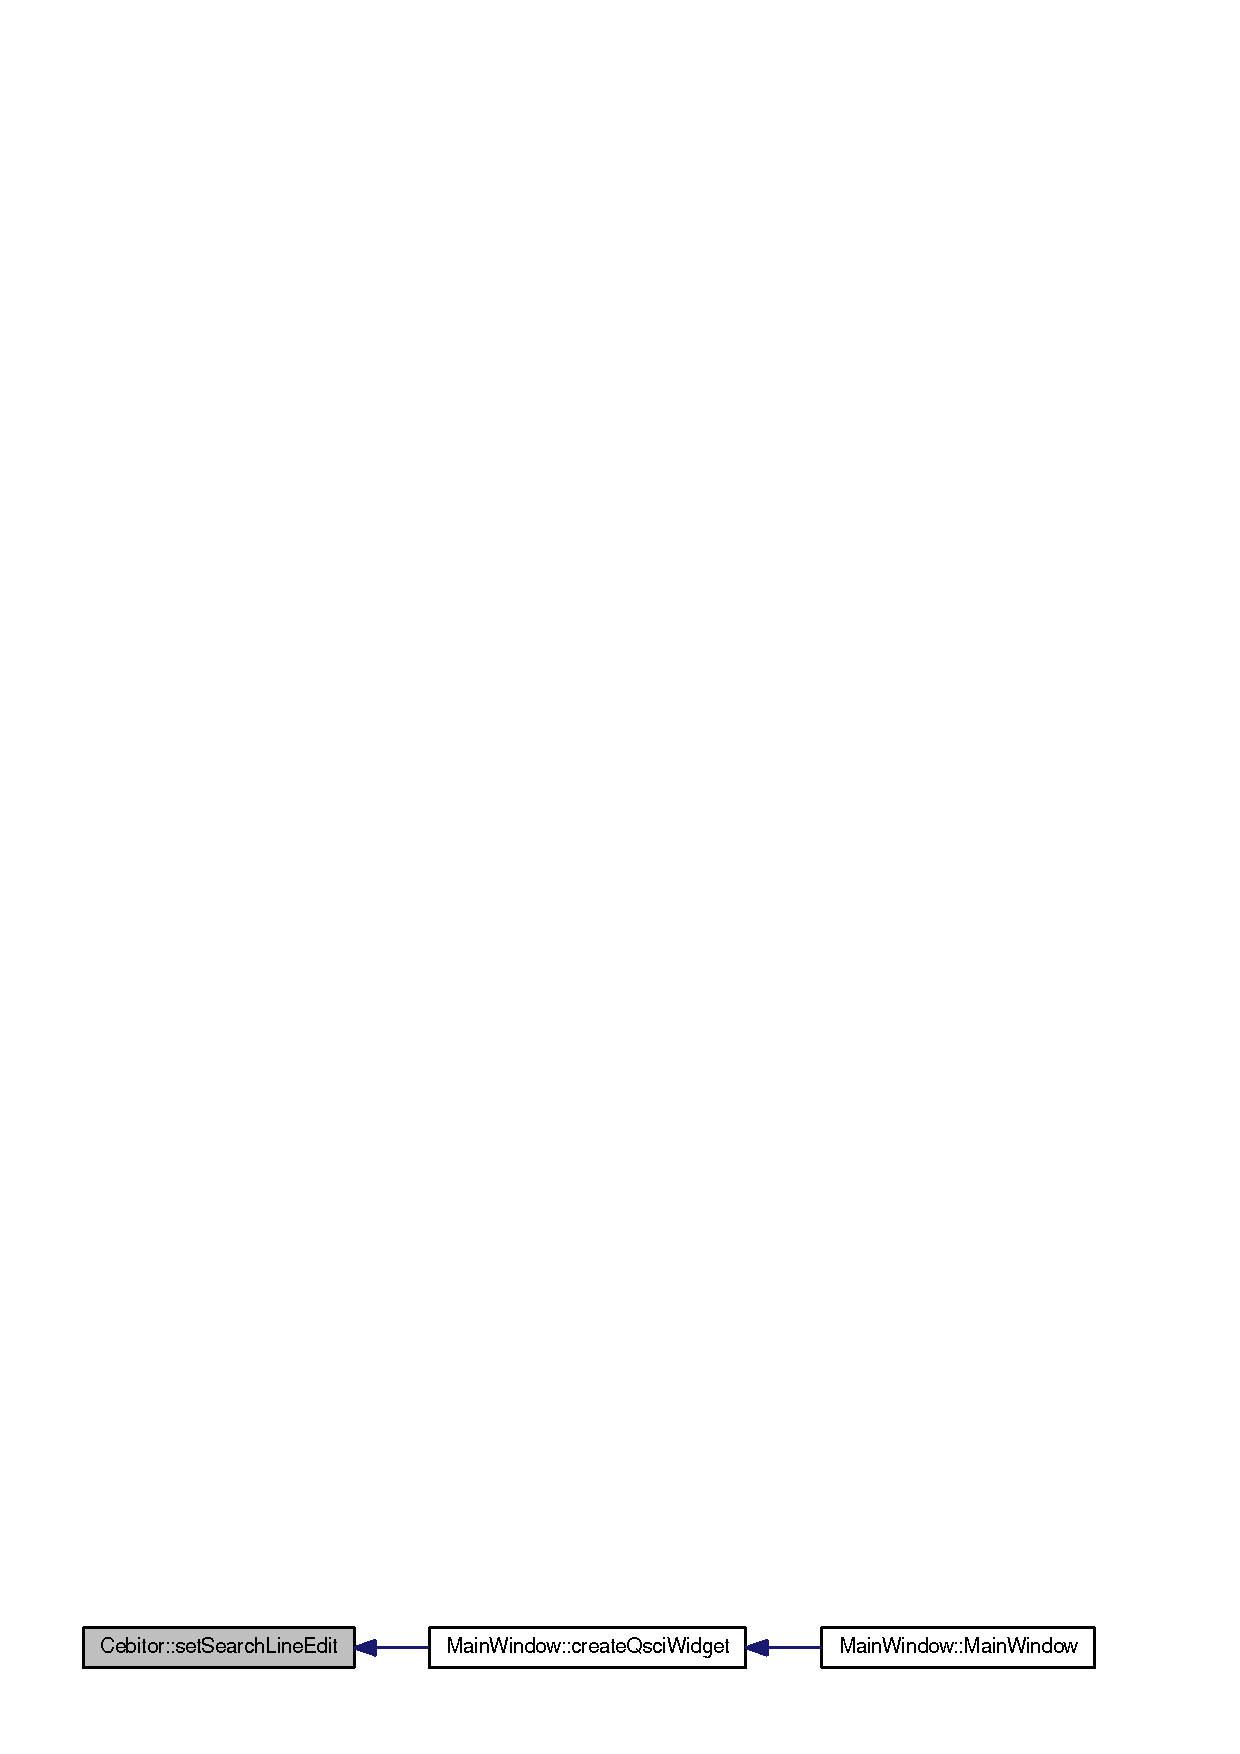
\includegraphics[width=350pt]{class_cebitor_a395cc168f396df26fd1fa20ae88dd44c_icgraph}
\end{center}
\end{figure}


\index{Cebitor@{Cebitor}!set\-Search\-Widget@{set\-Search\-Widget}}
\index{set\-Search\-Widget@{set\-Search\-Widget}!Cebitor@{Cebitor}}
\subsubsection[{set\-Search\-Widget}]{\setlength{\rightskip}{0pt plus 5cm}void Cebitor\-::set\-Search\-Widget (
\begin{DoxyParamCaption}
\item[{Q\-Widget $\ast$}]{\-\_\-search\-Widget}
\end{DoxyParamCaption}
)\hspace{0.3cm}{\ttfamily [inline]}}\label{class_cebitor_a1b38824f5bba6001688107ae901c14e7}


stores widget containing the searchbar 



Definition at line 42 of file Cebitor.\-h.



References m\-\_\-search\-Widget.


\begin{DoxyCode}
43                               \{
44                                 m_searchWidget = \_searchWidget;
45                               \}
\end{DoxyCode}


Here is the caller graph for this function\-:\nopagebreak
\begin{figure}[H]
\begin{center}
\leavevmode
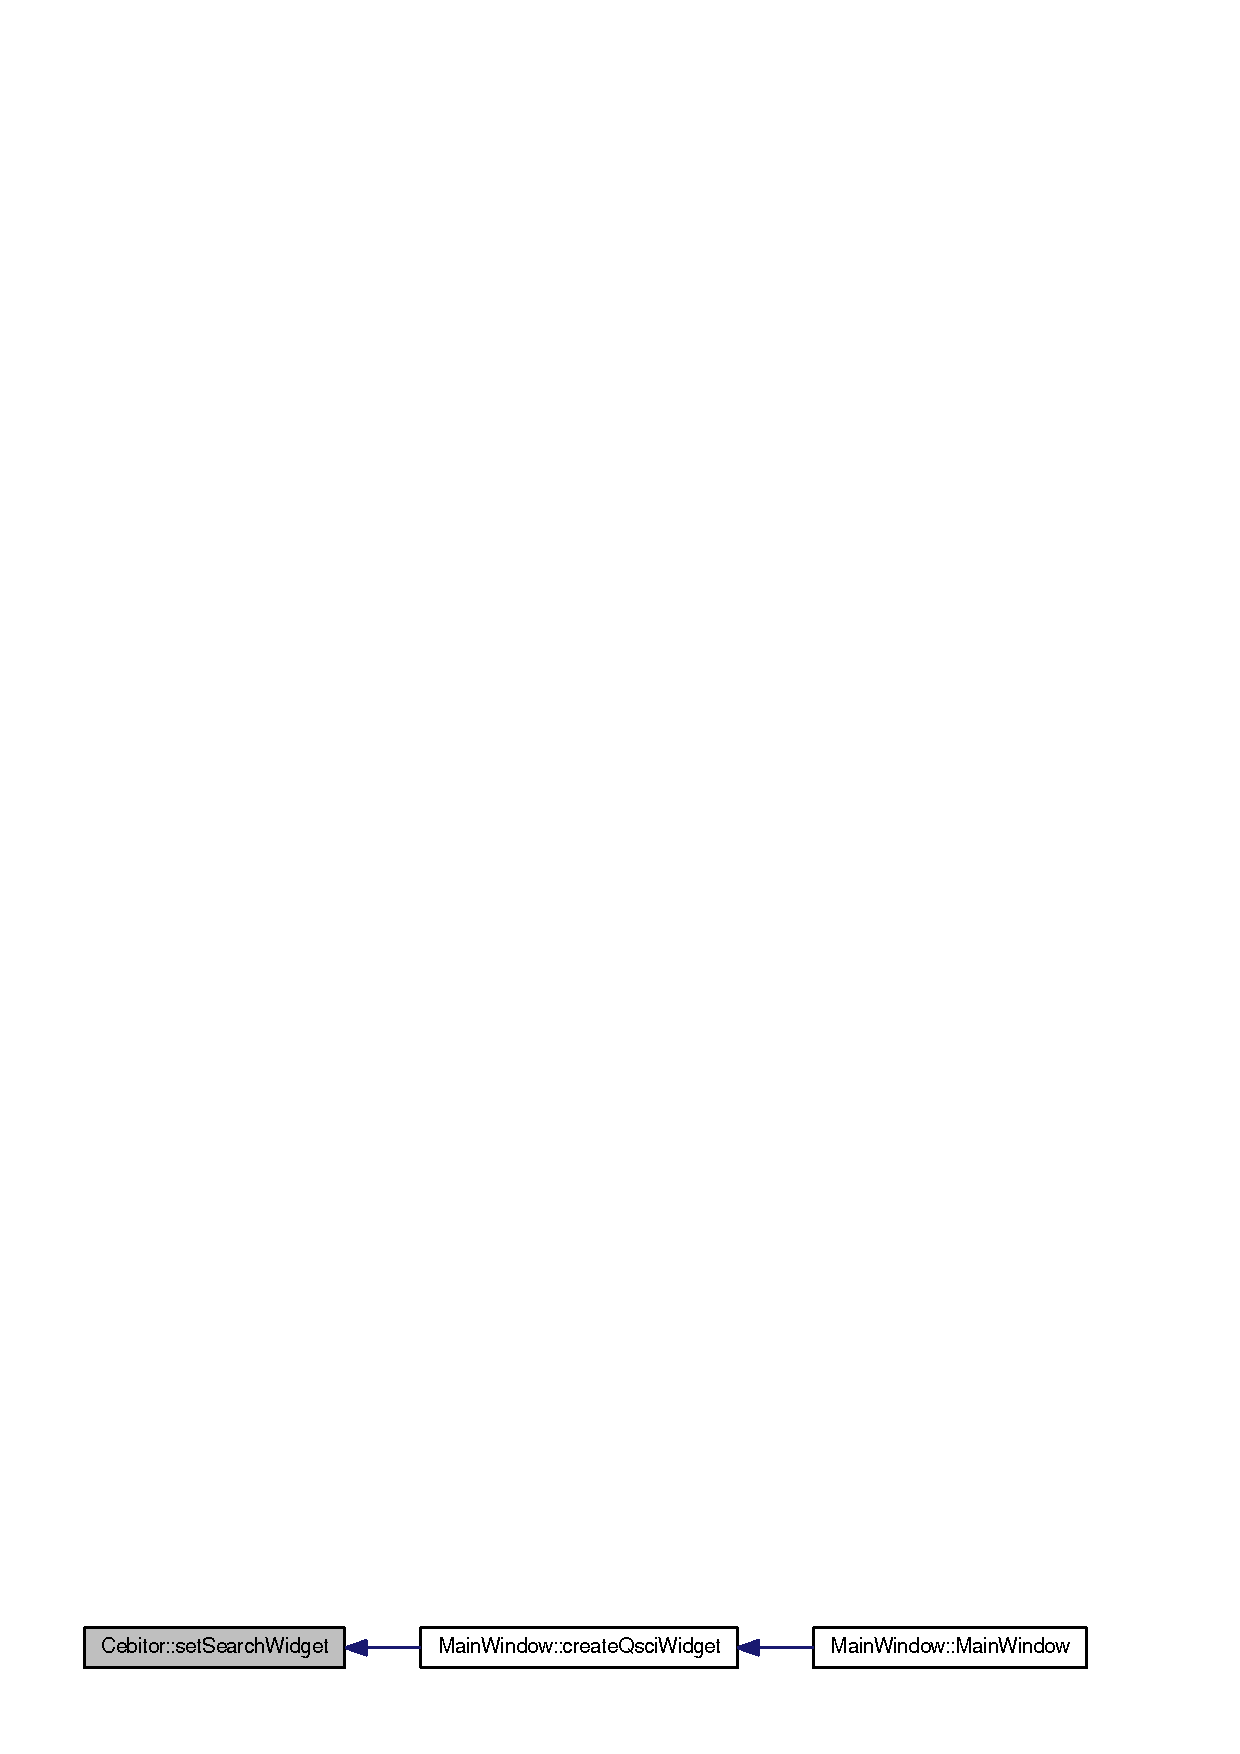
\includegraphics[width=350pt]{class_cebitor_a1b38824f5bba6001688107ae901c14e7_icgraph}
\end{center}
\end{figure}


\index{Cebitor@{Cebitor}!toggle\-Search\-Box@{toggle\-Search\-Box}}
\index{toggle\-Search\-Box@{toggle\-Search\-Box}!Cebitor@{Cebitor}}
\subsubsection[{toggle\-Search\-Box}]{\setlength{\rightskip}{0pt plus 5cm}void Cebitor\-::toggle\-Search\-Box (
\begin{DoxyParamCaption}
{}
\end{DoxyParamCaption}
)\hspace{0.3cm}{\ttfamily [protected]}, {\ttfamily [slot]}}\label{class_cebitor_a7d1825b3c849b79a9e7c559c312dd92a}


toggle search widget 



Definition at line 303 of file Cebitor.\-cpp.



References highlight\-All\-Search(), m\-\_\-search\-Indicator, m\-\_\-search\-Line\-Edit, and m\-\_\-search\-Widget.


\begin{DoxyCode}
304 \{
305   \textcolor{keywordtype}{bool} searchFocus = m_searchLineEdit->hasFocus();
306   \textcolor{keywordflow}{if}(!searchFocus)
307   \{
308     connect(\textcolor{keyword}{this},SIGNAL(textChanged()),\textcolor{keyword}{this},SLOT(highlightAllSearch()));
309     m_searchWidget->show();
310     m_searchLineEdit->setFocus();
311   \}
312   \textcolor{keywordflow}{else}
313   \{
314     disconnect(\textcolor{keyword}{this},SIGNAL(textChanged()),\textcolor{keyword}{this},SLOT(highlightAllSearch()));
315     m_searchWidget->hide();
316     setFocus();
317     clearIndicatorRange(0,0,lines(),text(lines()).length(),m_searchIndicator);
318   \}
319 \}
\end{DoxyCode}


Here is the call graph for this function\-:\nopagebreak
\begin{figure}[H]
\begin{center}
\leavevmode
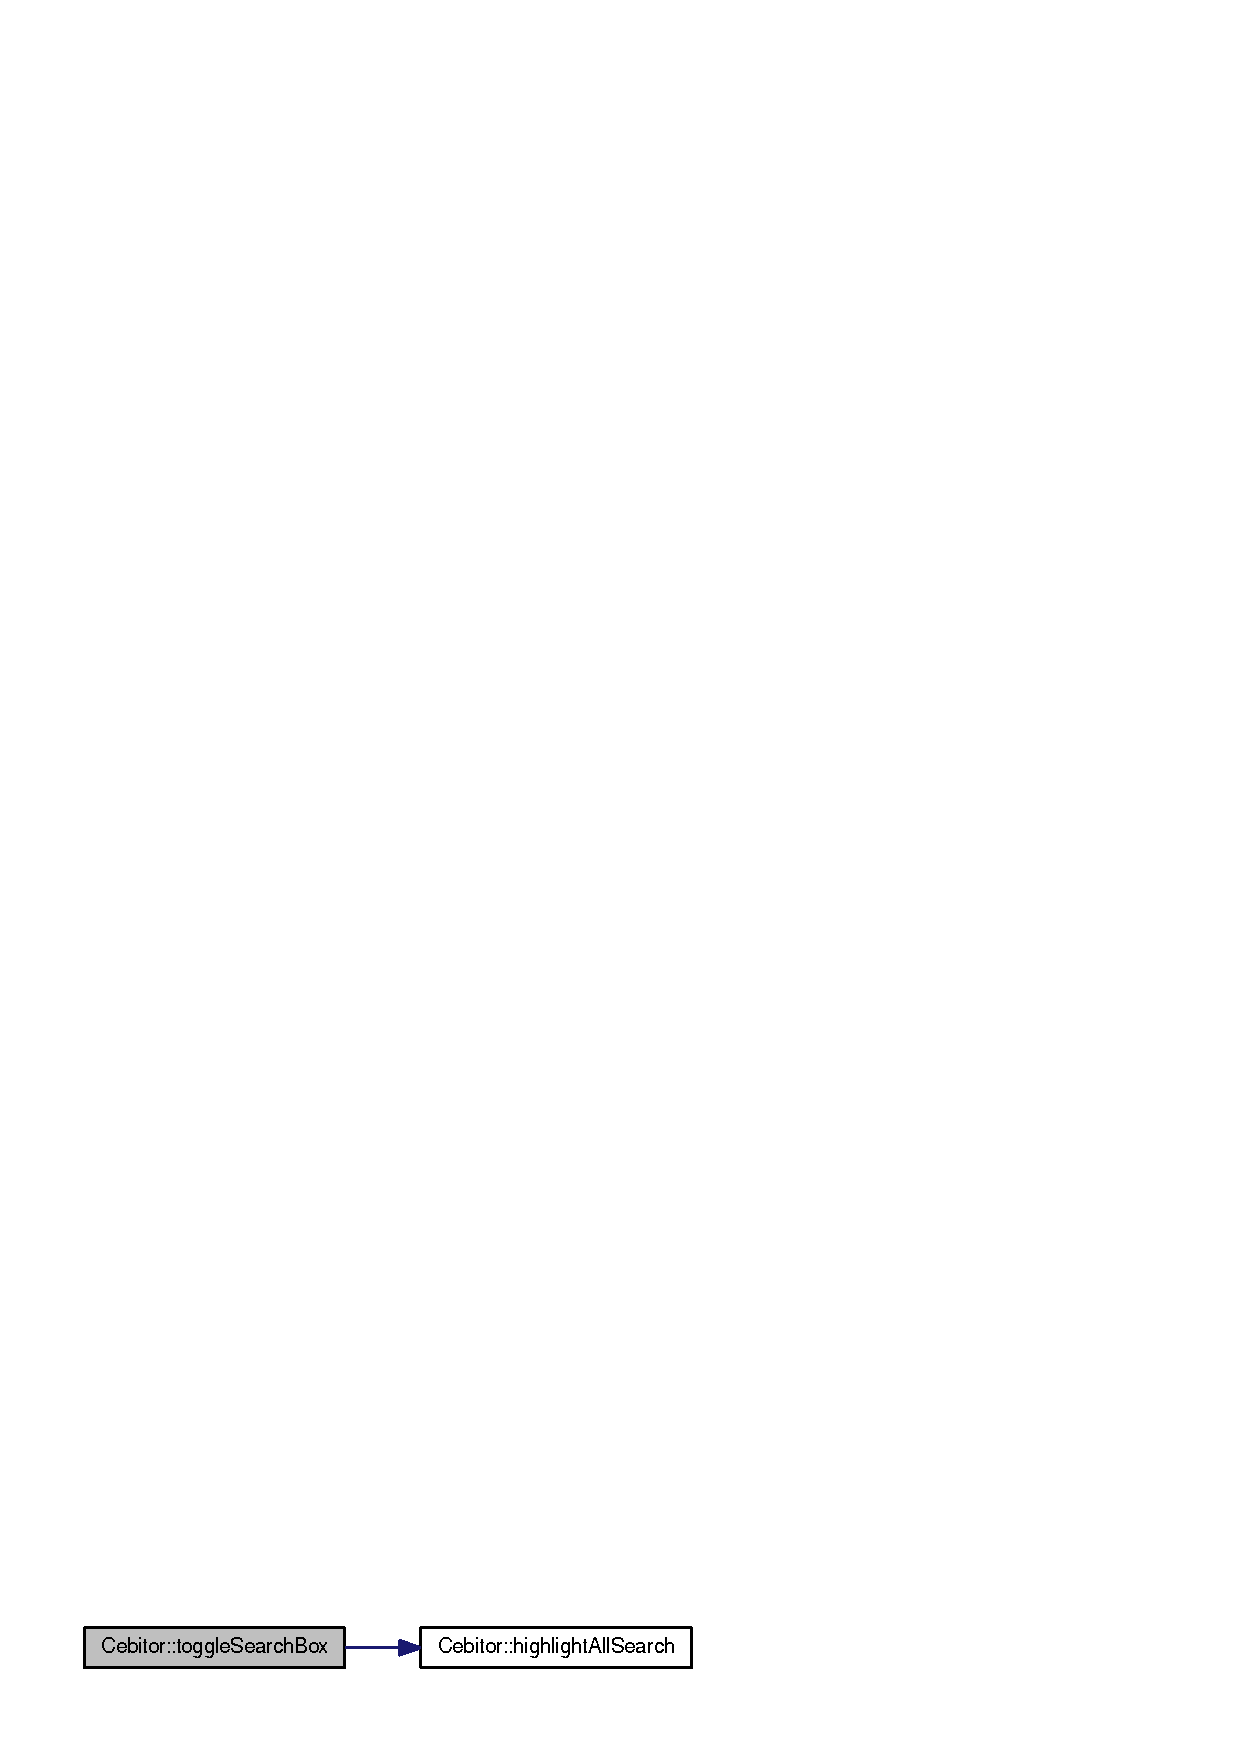
\includegraphics[width=336pt]{class_cebitor_a7d1825b3c849b79a9e7c559c312dd92a_cgraph}
\end{center}
\end{figure}




Here is the caller graph for this function\-:\nopagebreak
\begin{figure}[H]
\begin{center}
\leavevmode
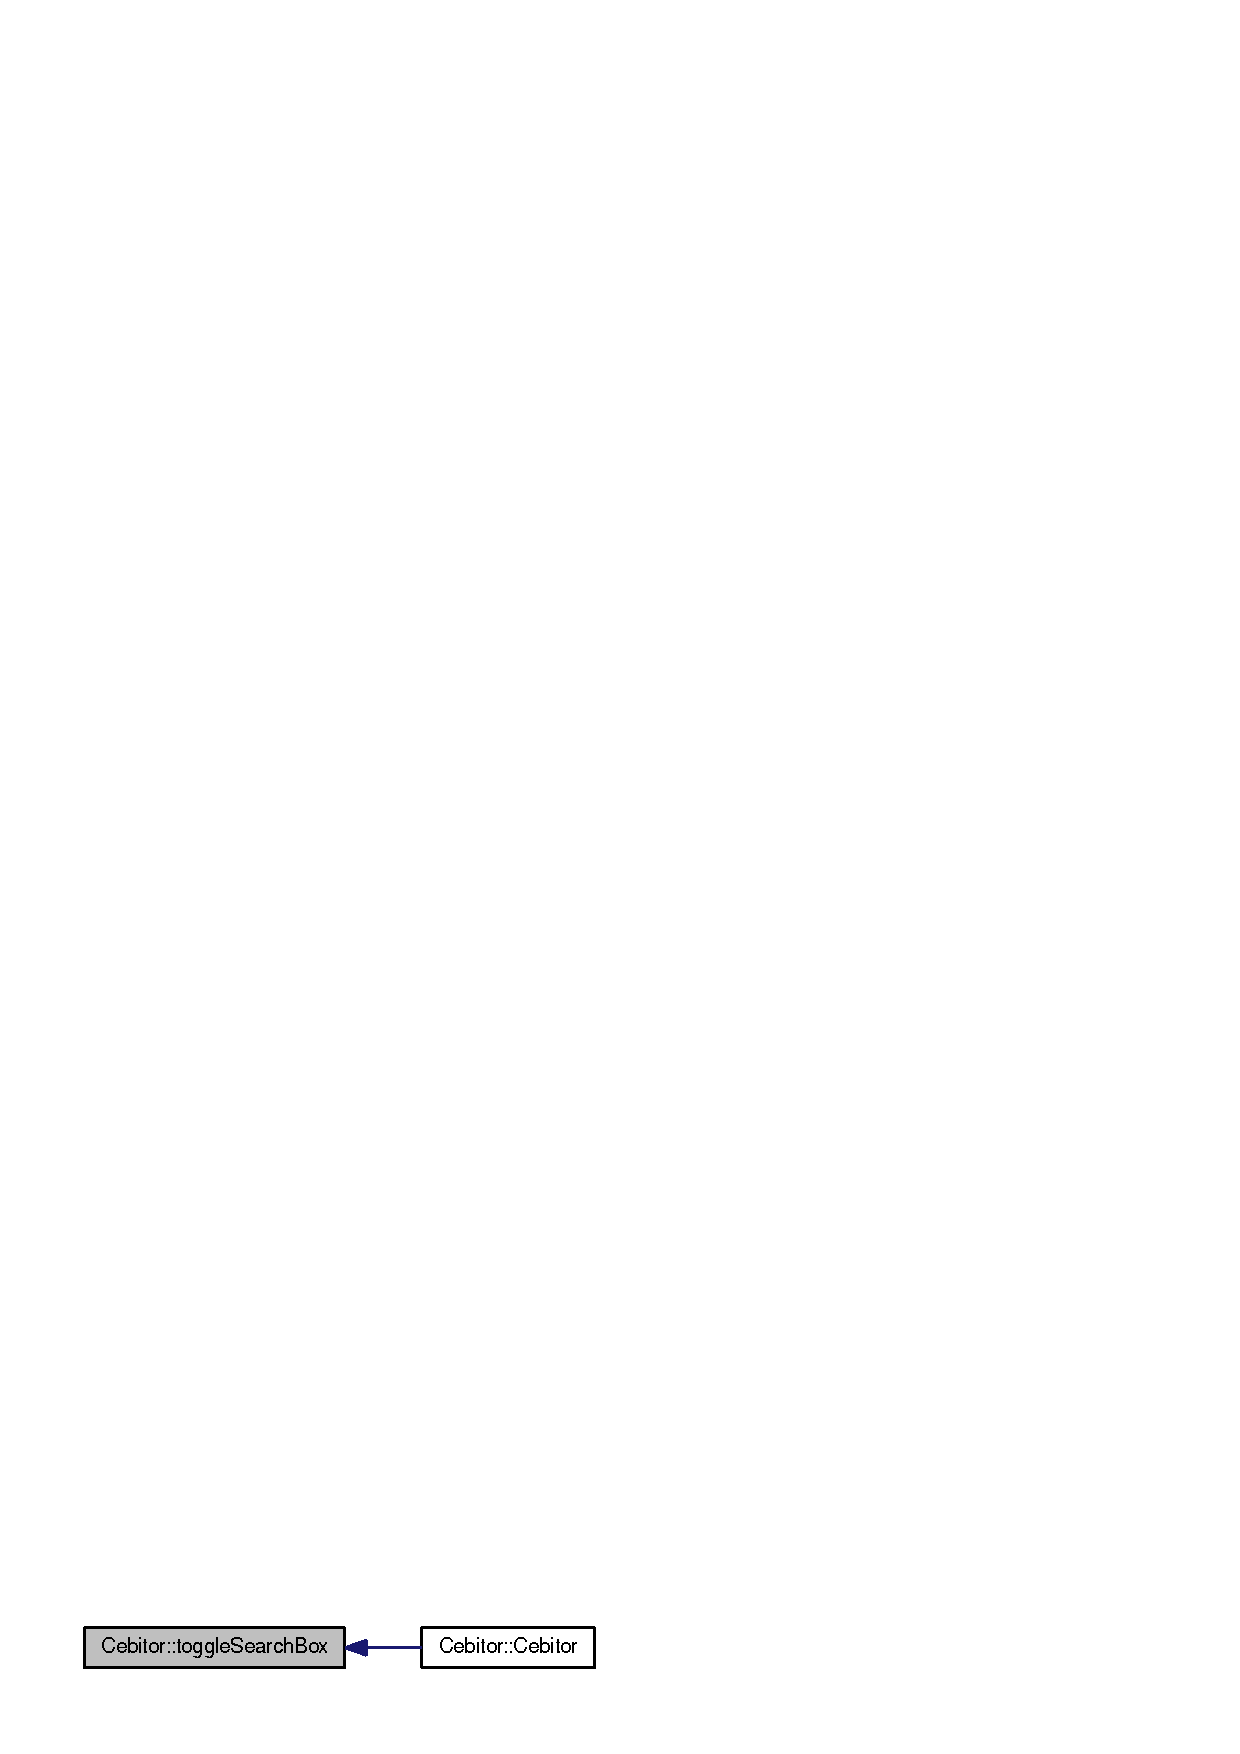
\includegraphics[width=290pt]{class_cebitor_a7d1825b3c849b79a9e7c559c312dd92a_icgraph}
\end{center}
\end{figure}




\subsection{Member Data Documentation}
\index{Cebitor@{Cebitor}!m\-\_\-file\-Markers@{m\-\_\-file\-Markers}}
\index{m\-\_\-file\-Markers@{m\-\_\-file\-Markers}!Cebitor@{Cebitor}}
\subsubsection[{m\-\_\-file\-Markers}]{\setlength{\rightskip}{0pt plus 5cm}std\-::vector$<$int$>$ Cebitor\-::m\-\_\-file\-Markers\hspace{0.3cm}{\ttfamily [protected]}}\label{class_cebitor_a13801a0fbdb375f7eab12003a6fd0dfc}


vector of all line markers 



Definition at line 90 of file Cebitor.\-h.

\index{Cebitor@{Cebitor}!m\-\_\-search\-Indicator@{m\-\_\-search\-Indicator}}
\index{m\-\_\-search\-Indicator@{m\-\_\-search\-Indicator}!Cebitor@{Cebitor}}
\subsubsection[{m\-\_\-search\-Indicator}]{\setlength{\rightskip}{0pt plus 5cm}int Cebitor\-::m\-\_\-search\-Indicator\hspace{0.3cm}{\ttfamily [protected]}}\label{class_cebitor_abc185ddfb53d0479826e995157dd559b}


indicator used to highlight all search terms 



Definition at line 94 of file Cebitor.\-h.

\index{Cebitor@{Cebitor}!m\-\_\-search\-Line\-Edit@{m\-\_\-search\-Line\-Edit}}
\index{m\-\_\-search\-Line\-Edit@{m\-\_\-search\-Line\-Edit}!Cebitor@{Cebitor}}
\subsubsection[{m\-\_\-search\-Line\-Edit}]{\setlength{\rightskip}{0pt plus 5cm}Q\-Line\-Edit$\ast$ Cebitor\-::m\-\_\-search\-Line\-Edit\hspace{0.3cm}{\ttfamily [protected]}}\label{class_cebitor_a6e8510e102fc4e2796b5f115c5141469}


searchbar Q\-Line\-Edit widget 



Definition at line 86 of file Cebitor.\-h.

\index{Cebitor@{Cebitor}!m\-\_\-search\-Widget@{m\-\_\-search\-Widget}}
\index{m\-\_\-search\-Widget@{m\-\_\-search\-Widget}!Cebitor@{Cebitor}}
\subsubsection[{m\-\_\-search\-Widget}]{\setlength{\rightskip}{0pt plus 5cm}Q\-Widget$\ast$ Cebitor\-::m\-\_\-search\-Widget\hspace{0.3cm}{\ttfamily [protected]}}\label{class_cebitor_ae864f4361408ef8db8c4e91e8c464524}


widget containing the searchbar 



Definition at line 82 of file Cebitor.\-h.



The documentation for this class was generated from the following files\-:\begin{DoxyCompactItemize}
\item 
{\bf Cebitor.\-h}\item 
{\bf Cebitor.\-cpp}\end{DoxyCompactItemize}

\section{Colour\-Button Class Reference}
\label{class_colour_button}\index{Colour\-Button@{Colour\-Button}}


\doxyref{Button}{p.}{class_button} to set colour uniform values.  




{\ttfamily \#include $<$Button.\-h$>$}



Inheritance diagram for Colour\-Button\-:
\nopagebreak
\begin{figure}[H]
\begin{center}
\leavevmode
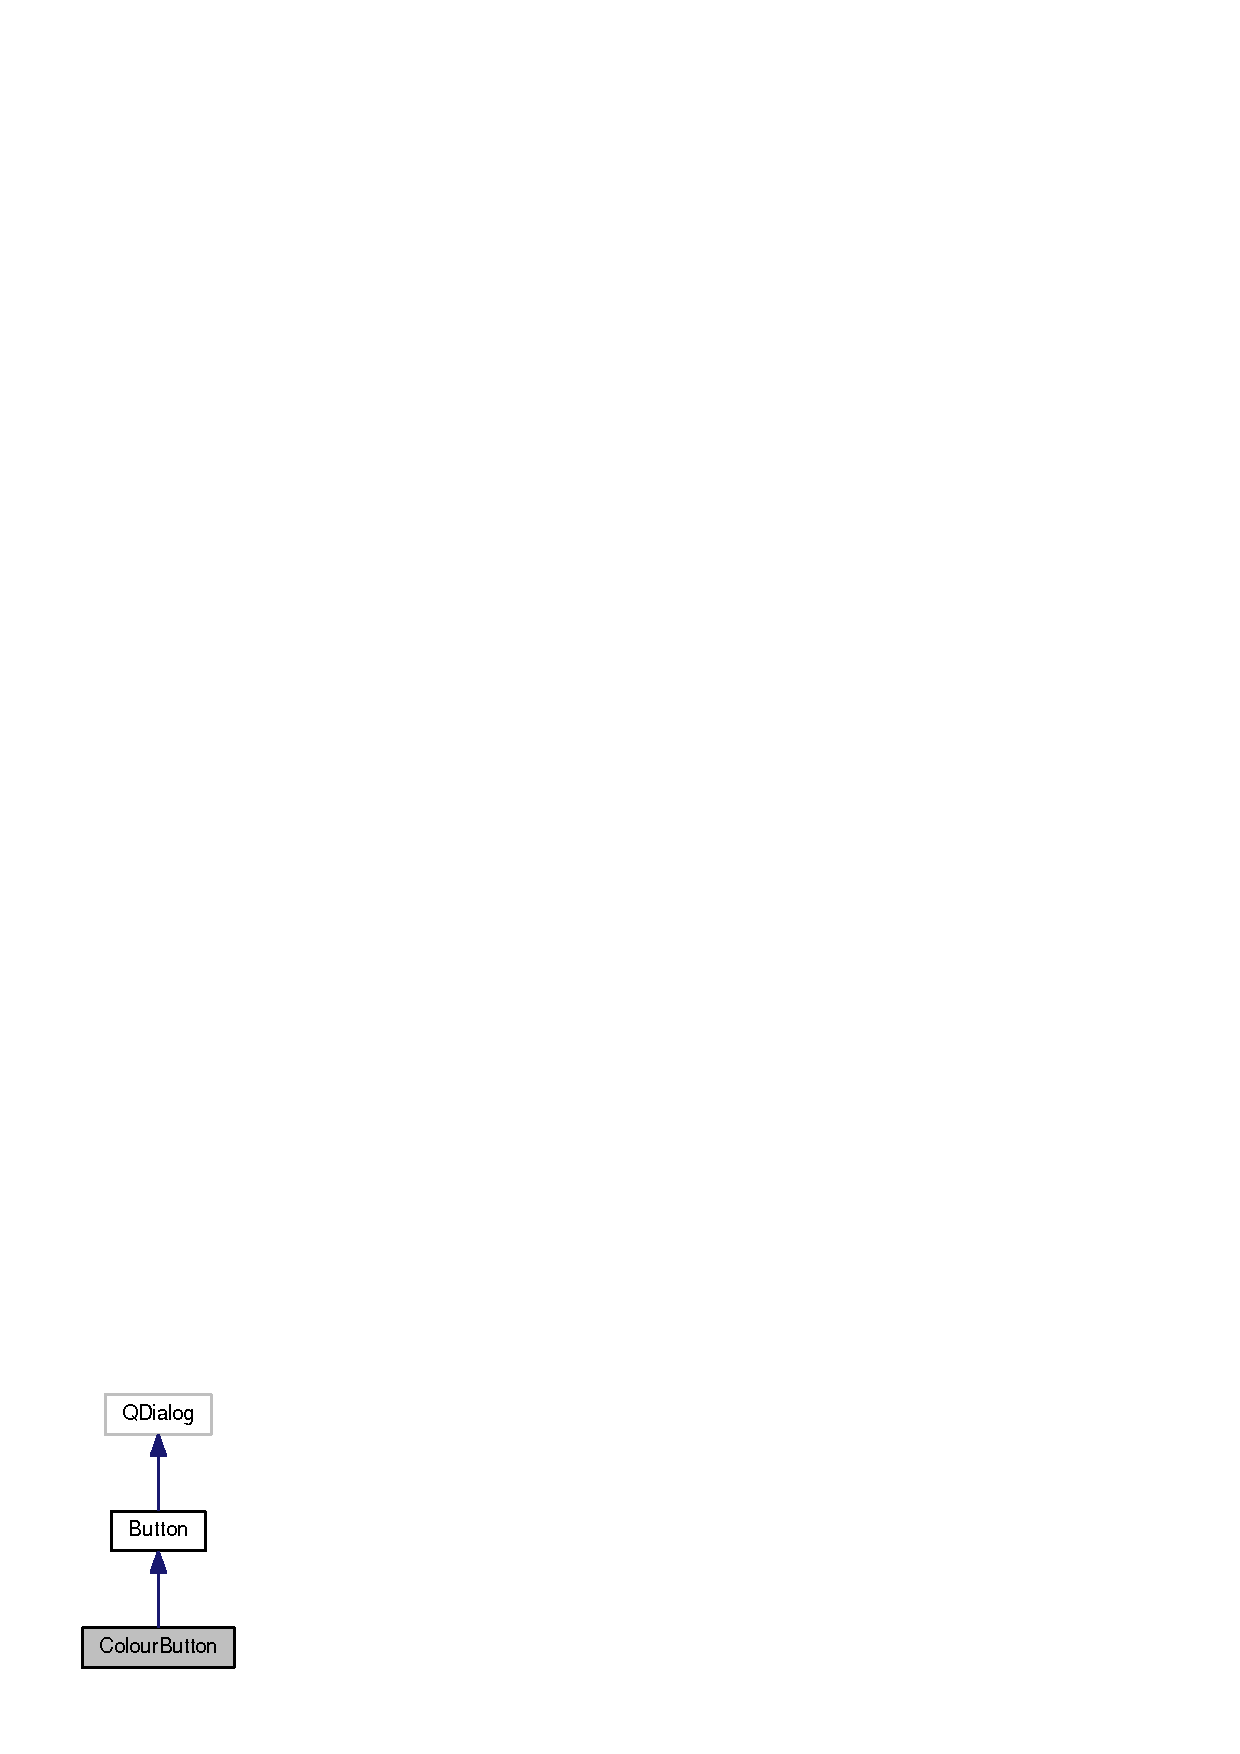
\includegraphics[width=116pt]{class_colour_button__inherit__graph}
\end{center}
\end{figure}


Collaboration diagram for Colour\-Button\-:
\nopagebreak
\begin{figure}[H]
\begin{center}
\leavevmode
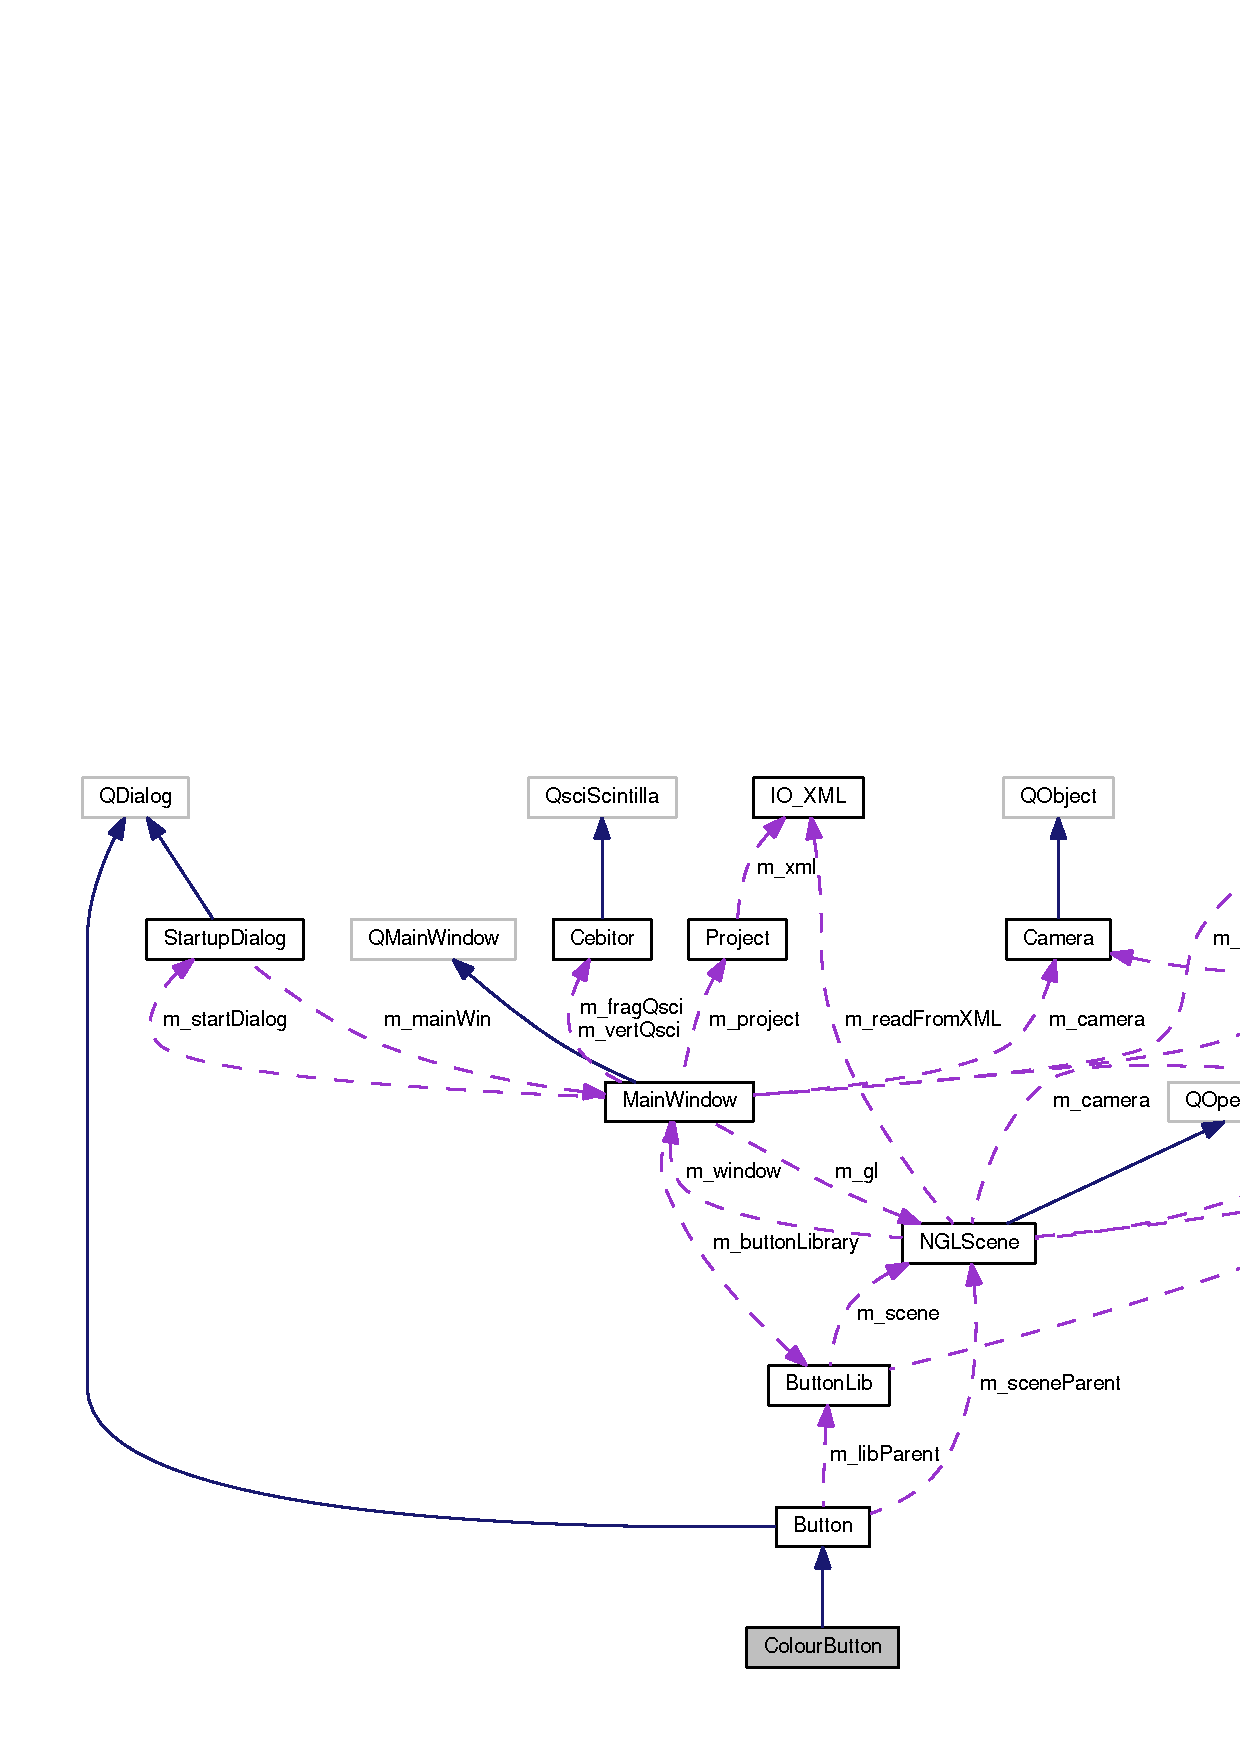
\includegraphics[width=350pt]{class_colour_button__coll__graph}
\end{center}
\end{figure}
\subsection*{Public Member Functions}
\begin{DoxyCompactItemize}
\item 
void {\bf set\-Colour} (Q\-Color \-\_\-col)
\begin{DoxyCompactList}\small\item\em sets the picked colour and colour attribute to the colour input \end{DoxyCompactList}\item 
void {\bf set\-Colour} (ngl\-::\-Vec4 \-\_\-col)
\begin{DoxyCompactList}\small\item\em sets the colour attribute to the colour input \end{DoxyCompactList}\item 
ngl\-::\-Vec4 {\bf get\-Colour} ()
\begin{DoxyCompactList}\small\item\em returns the colour, stored by the button \end{DoxyCompactList}\item 
Q\-Color {\bf get\-Colour\-Q} ()
\begin{DoxyCompactList}\small\item\em returns the Q\-Color, stored by the button \end{DoxyCompactList}\item 
void {\bf print\-Attributes} ()
\begin{DoxyCompactList}\small\item\em print the attribute data stored within the colour attriubte for debugging \end{DoxyCompactList}\end{DoxyCompactItemize}
\subsection*{Private Slots}
\begin{DoxyCompactItemize}
\item 
void {\bf open\-Box} ()
\begin{DoxyCompactList}\small\item\em a slot to open a colour widget upon button press event \end{DoxyCompactList}\end{DoxyCompactItemize}
\subsection*{Private Attributes}
\begin{DoxyCompactItemize}
\item 
ngl\-::\-Vec4 {\bf m\-\_\-colour}
\begin{DoxyCompactList}\small\item\em vector to store colour attributes \end{DoxyCompactList}\item 
Q\-Color {\bf m\-\_\-colour\-Picked}
\begin{DoxyCompactList}\small\item\em colour used to store attributes from colour picker \end{DoxyCompactList}\item 
Q\-Color\-Dialog $\ast$ {\bf m\-\_\-colour\-Group\-Box}
\begin{DoxyCompactList}\small\item\em colour box to select colours \end{DoxyCompactList}\end{DoxyCompactItemize}
\subsection*{Additional Inherited Members}


\subsection{Detailed Description}
\doxyref{Button}{p.}{class_button} to set colour uniform values. 

Definition at line 191 of file Button.\-h.



\subsection{Member Function Documentation}
\index{Colour\-Button@{Colour\-Button}!get\-Colour@{get\-Colour}}
\index{get\-Colour@{get\-Colour}!ColourButton@{Colour\-Button}}
\subsubsection[{get\-Colour}]{\setlength{\rightskip}{0pt plus 5cm}ngl\-::\-Vec4 Colour\-Button\-::get\-Colour (
\begin{DoxyParamCaption}
{}
\end{DoxyParamCaption}
)\hspace{0.3cm}{\ttfamily [inline]}, {\ttfamily [virtual]}}\label{class_colour_button_ab16ef6ea899d28e8b8a8500d95a5d188}


returns the colour, stored by the button 

\begin{DoxyReturn}{Returns}
m\-\_\-colour 
\end{DoxyReturn}


Reimplemented from {\bf Button} \doxyref{}{p.}{class_button_a70975849d59dca023bd95047dfd0771e}.



Definition at line 214 of file Button.\-h.



References m\-\_\-colour.


\begin{DoxyCode}
214 \{\textcolor{keywordflow}{return} m_colour;\}
\end{DoxyCode}
\index{Colour\-Button@{Colour\-Button}!get\-Colour\-Q@{get\-Colour\-Q}}
\index{get\-Colour\-Q@{get\-Colour\-Q}!ColourButton@{Colour\-Button}}
\subsubsection[{get\-Colour\-Q}]{\setlength{\rightskip}{0pt plus 5cm}Q\-Color Colour\-Button\-::get\-Colour\-Q (
\begin{DoxyParamCaption}
{}
\end{DoxyParamCaption}
)\hspace{0.3cm}{\ttfamily [inline]}, {\ttfamily [virtual]}}\label{class_colour_button_a3063b9d295eb8f9f0a0f69726f2c9449}


returns the Q\-Color, stored by the button 

\begin{DoxyReturn}{Returns}
m\-\_\-colour\-Picked 
\end{DoxyReturn}


Reimplemented from {\bf Button} \doxyref{}{p.}{class_button_aca34c082733f62c47cee7e278b3ae876}.



Definition at line 219 of file Button.\-h.



References m\-\_\-colour\-Picked.


\begin{DoxyCode}
219 \{\textcolor{keywordflow}{return} m_colourPicked;\}
\end{DoxyCode}
\index{Colour\-Button@{Colour\-Button}!open\-Box@{open\-Box}}
\index{open\-Box@{open\-Box}!ColourButton@{Colour\-Button}}
\subsubsection[{open\-Box}]{\setlength{\rightskip}{0pt plus 5cm}void Colour\-Button\-::open\-Box (
\begin{DoxyParamCaption}
{}
\end{DoxyParamCaption}
)\hspace{0.3cm}{\ttfamily [private]}, {\ttfamily [slot]}}\label{class_colour_button_a88b25c33088480a429c75028fbf61b54}


a slot to open a colour widget upon button press event 



Definition at line 47 of file Button.\-cpp.



References m\-\_\-colour, m\-\_\-colour\-Group\-Box, m\-\_\-colour\-Picked, Button\-::m\-\_\-lib\-Parent, Button\-::m\-\_\-parent, Button\-::m\-\_\-scene\-Parent, and Button\-Lib\-::update\-Shader\-Values().


\begin{DoxyCode}
48 \{
49   \textcolor{comment}{//these are set so when the colour picker is opened the current colour is opened}
50   m_colourPicked.setRedF(m_colour.m\_x);
51   m_colourPicked.setGreenF(m_colour.m\_y);
52   m_colourPicked.setBlueF(m_colour.m\_z);
53   m_colourPicked=m_colourGroupBox->getColor(m_colourPicked,
54                                             m_parent,
55                                             \textcolor{stringliteral}{"Pick a colour"},
56                                             0);
57   \textcolor{keywordflow}{if}(m_colourPicked.spec()!=QColor::Spec::Invalid)
58   \{
59     m_colour.set(m_colourPicked.redF(),
60                  m_colourPicked.greenF(),
61                  m_colourPicked.blueF(),
62                  m_colourPicked.alphaF());
63     m_libParent->updateShaderValues();
64     m_sceneParent->update();
65   \}
66 
67 \}
\end{DoxyCode}


Here is the call graph for this function\-:
\nopagebreak
\begin{figure}[H]
\begin{center}
\leavevmode
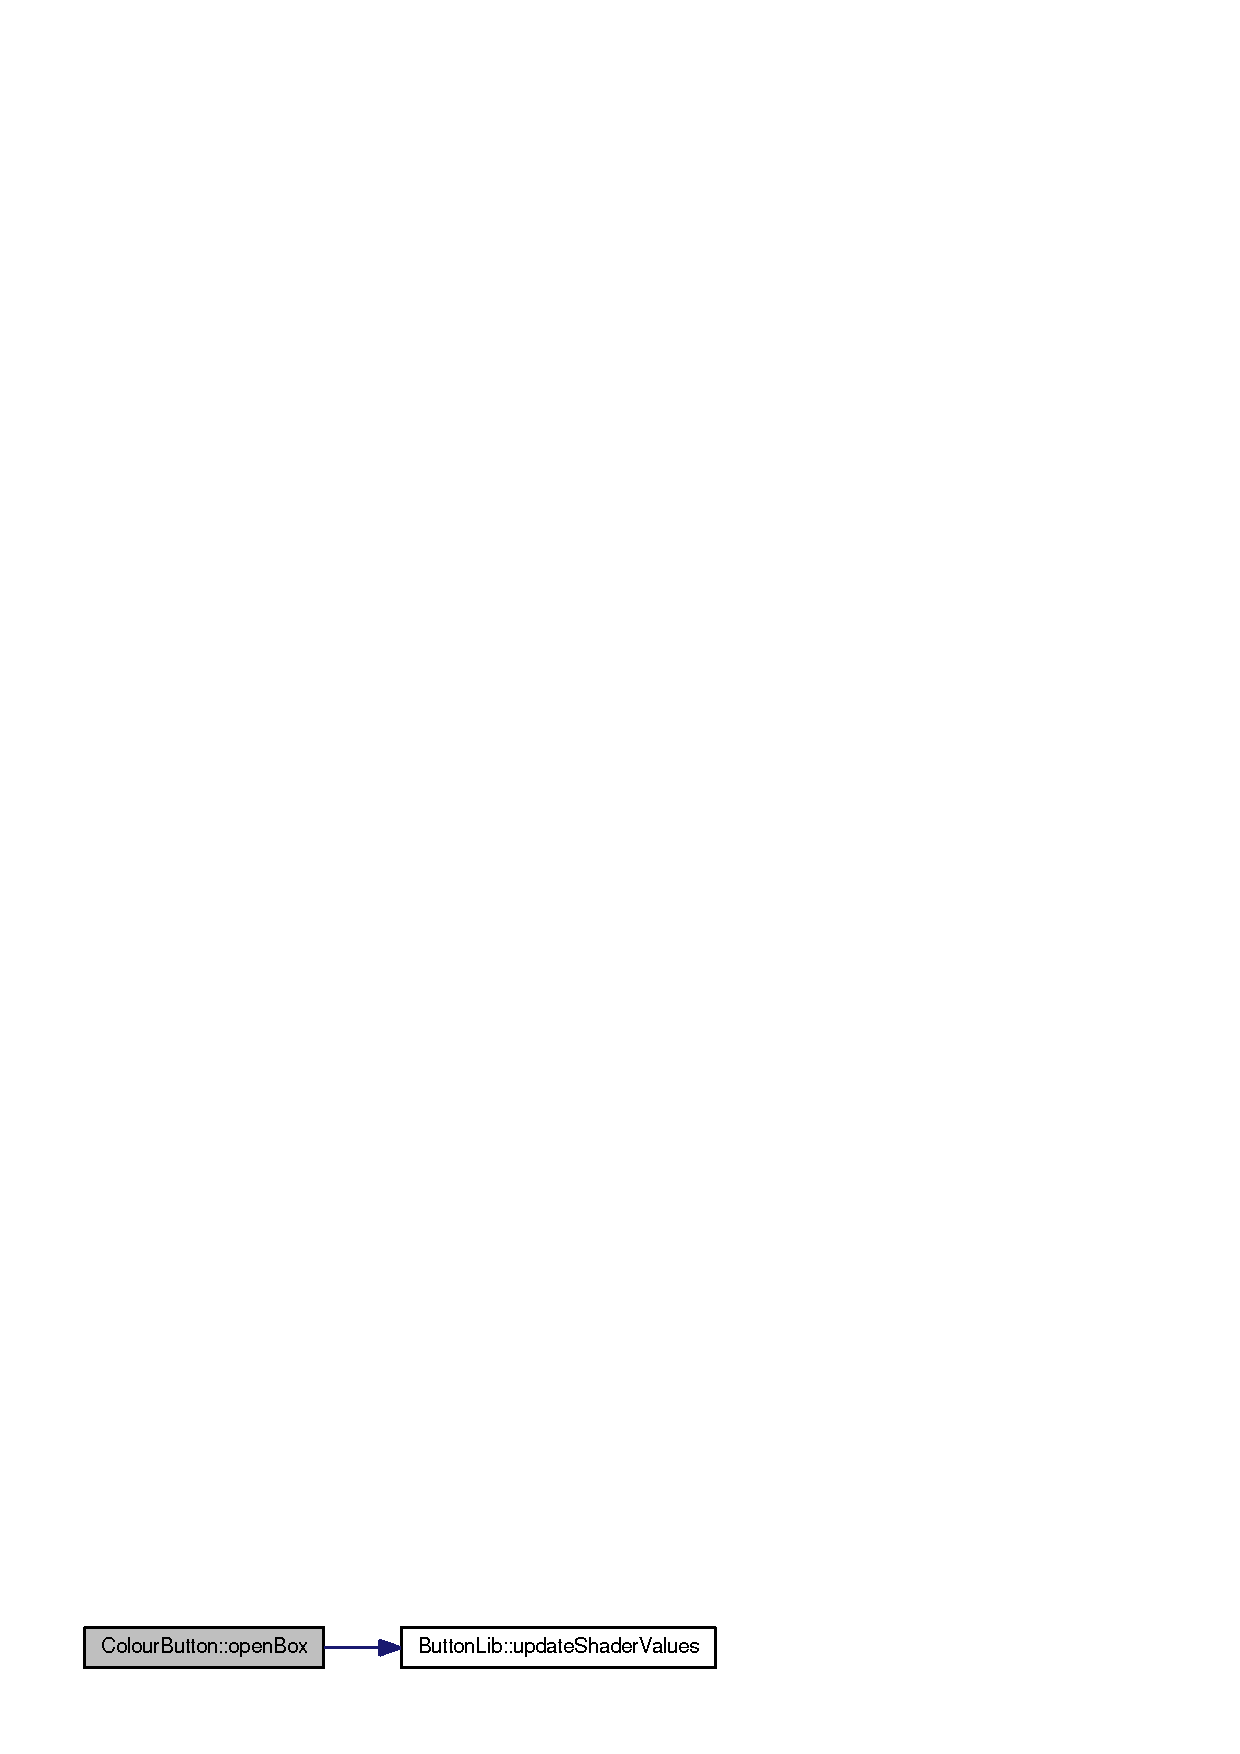
\includegraphics[width=348pt]{class_colour_button_a88b25c33088480a429c75028fbf61b54_cgraph}
\end{center}
\end{figure}


\index{Colour\-Button@{Colour\-Button}!print\-Attributes@{print\-Attributes}}
\index{print\-Attributes@{print\-Attributes}!ColourButton@{Colour\-Button}}
\subsubsection[{print\-Attributes}]{\setlength{\rightskip}{0pt plus 5cm}void Colour\-Button\-::print\-Attributes (
\begin{DoxyParamCaption}
{}
\end{DoxyParamCaption}
)}\label{class_colour_button_a7a5950e9b6c326ed32125868f0765792}


print the attribute data stored within the colour attriubte for debugging 



Definition at line 42 of file Button.\-cpp.



References m\-\_\-colour.


\begin{DoxyCode}
43 \{
44   std::cout<<\textcolor{stringliteral}{"R: "}<<m_colour.m\_x<<\textcolor{stringliteral}{"\(\backslash\)nG: "}<<m_colour.m\_y<<\textcolor{stringliteral}{"\(\backslash\)nB: "}<<m_colour.m\_z<<std::endl;
45 \}
\end{DoxyCode}
\index{Colour\-Button@{Colour\-Button}!set\-Colour@{set\-Colour}}
\index{set\-Colour@{set\-Colour}!ColourButton@{Colour\-Button}}
\subsubsection[{set\-Colour}]{\setlength{\rightskip}{0pt plus 5cm}void Colour\-Button\-::set\-Colour (
\begin{DoxyParamCaption}
\item[{Q\-Color}]{\-\_\-col}
\end{DoxyParamCaption}
)\hspace{0.3cm}{\ttfamily [virtual]}}\label{class_colour_button_a1702284d1cdfe7bff2db19e219132f37}


sets the picked colour and colour attribute to the colour input 


\begin{DoxyParams}[1]{Parameters}
\mbox{\tt in}  & {\em colour} & value \\
\hline
\end{DoxyParams}


Reimplemented from {\bf Button} \doxyref{}{p.}{class_button_a174b05c6f309a46db10530052cf8388a}.



Definition at line 69 of file Button.\-cpp.



References m\-\_\-colour, and m\-\_\-colour\-Picked.


\begin{DoxyCode}
70 \{
71   m_colourPicked=\_col;
72   m_colour.set(\_col.redF(),
73                \_col.greenF(),
74                \_col.blueF(),
75                \_col.alphaF());
76 \}
\end{DoxyCode}


Here is the caller graph for this function\-:
\nopagebreak
\begin{figure}[H]
\begin{center}
\leavevmode
\includegraphics[width=350pt]{class_colour_button_a1702284d1cdfe7bff2db19e219132f37_icgraph}
\end{center}
\end{figure}


\index{Colour\-Button@{Colour\-Button}!set\-Colour@{set\-Colour}}
\index{set\-Colour@{set\-Colour}!ColourButton@{Colour\-Button}}
\subsubsection[{set\-Colour}]{\setlength{\rightskip}{0pt plus 5cm}void Colour\-Button\-::set\-Colour (
\begin{DoxyParamCaption}
\item[{ngl\-::\-Vec4}]{\-\_\-col}
\end{DoxyParamCaption}
)\hspace{0.3cm}{\ttfamily [virtual]}}\label{class_colour_button_abb4011f8d6d85856a2ee155817b52135}


sets the colour attribute to the colour input 


\begin{DoxyParams}[1]{Parameters}
\mbox{\tt in}  & {\em colour} & value \\
\hline
\end{DoxyParams}


Reimplemented from {\bf Button} \doxyref{}{p.}{class_button_a339347e88020f2c961e08a530407d083}.



Definition at line 78 of file Button.\-cpp.



References m\-\_\-colour, and m\-\_\-colour\-Picked.


\begin{DoxyCode}
79 \{
80   m_colour=\_col;
81   m_colourPicked.setRgbF(m_colour.m\_x,
82                          m_colour.m\_y,
83                          m_colour.m\_z,
84                          m_colour.m\_w);
85 \}
\end{DoxyCode}


\subsection{Member Data Documentation}
\index{Colour\-Button@{Colour\-Button}!m\-\_\-colour@{m\-\_\-colour}}
\index{m\-\_\-colour@{m\-\_\-colour}!ColourButton@{Colour\-Button}}
\subsubsection[{m\-\_\-colour}]{\setlength{\rightskip}{0pt plus 5cm}ngl\-::\-Vec4 Colour\-Button\-::m\-\_\-colour\hspace{0.3cm}{\ttfamily [private]}}\label{class_colour_button_a40e0abfcdadcd7b2c249d275595c25a3}


vector to store colour attributes 



Definition at line 229 of file Button.\-h.

\index{Colour\-Button@{Colour\-Button}!m\-\_\-colour\-Group\-Box@{m\-\_\-colour\-Group\-Box}}
\index{m\-\_\-colour\-Group\-Box@{m\-\_\-colour\-Group\-Box}!ColourButton@{Colour\-Button}}
\subsubsection[{m\-\_\-colour\-Group\-Box}]{\setlength{\rightskip}{0pt plus 5cm}Q\-Color\-Dialog$\ast$ Colour\-Button\-::m\-\_\-colour\-Group\-Box\hspace{0.3cm}{\ttfamily [private]}}\label{class_colour_button_af654f70a6788a906c396d049cc85d628}


colour box to select colours 



Definition at line 237 of file Button.\-h.

\index{Colour\-Button@{Colour\-Button}!m\-\_\-colour\-Picked@{m\-\_\-colour\-Picked}}
\index{m\-\_\-colour\-Picked@{m\-\_\-colour\-Picked}!ColourButton@{Colour\-Button}}
\subsubsection[{m\-\_\-colour\-Picked}]{\setlength{\rightskip}{0pt plus 5cm}Q\-Color Colour\-Button\-::m\-\_\-colour\-Picked\hspace{0.3cm}{\ttfamily [private]}}\label{class_colour_button_a9105f23e49c6995233d42d3d028dd18a}


colour used to store attributes from colour picker 



Definition at line 233 of file Button.\-h.



The documentation for this class was generated from the following files\-:\begin{DoxyCompactItemize}
\item 
{\bf Button.\-h}\item 
{\bf Button.\-cpp}\end{DoxyCompactItemize}

\section{Conclusion\-Page Class Reference}
\label{class_conclusion_page}\index{Conclusion\-Page@{Conclusion\-Page}}


The final project wizard page that asks for confirmation to generate project.  




{\ttfamily \#include $<$New\-Project\-Wizard.\-h$>$}



Inheritance diagram for Conclusion\-Page\-:\nopagebreak
\begin{figure}[H]
\begin{center}
\leavevmode
\includegraphics[width=130pt]{class_conclusion_page__inherit__graph}
\end{center}
\end{figure}


Collaboration diagram for Conclusion\-Page\-:\nopagebreak
\begin{figure}[H]
\begin{center}
\leavevmode
\includegraphics[width=130pt]{class_conclusion_page__coll__graph}
\end{center}
\end{figure}
\subsection*{Public Member Functions}
\begin{DoxyCompactItemize}
\item 
{\bf Conclusion\-Page} (Q\-Widget $\ast$parent=0)
\begin{DoxyCompactList}\small\item\em Constructor, passing a child of parent. \end{DoxyCompactList}\end{DoxyCompactItemize}
\subsection*{Protected Member Functions}
\begin{DoxyCompactItemize}
\item 
void {\bf initialize\-Page} () Q\-\_\-\-D\-E\-C\-L\-\_\-\-O\-V\-E\-R\-R\-I\-D\-E
\begin{DoxyCompactList}\small\item\em Used to prepare the Wizard page before it is shown and set default values. \end{DoxyCompactList}\end{DoxyCompactItemize}
\subsection*{Private Attributes}
\begin{DoxyCompactItemize}
\item 
Q\-Label $\ast$ {\bf m\-\_\-label}
\begin{DoxyCompactList}\small\item\em The text label for the intro. \end{DoxyCompactList}\end{DoxyCompactItemize}


\subsection{Detailed Description}
The final project wizard page that asks for confirmation to generate project. 

Definition at line 365 of file New\-Project\-Wizard.\-h.



\subsection{Constructor \& Destructor Documentation}
\index{Conclusion\-Page@{Conclusion\-Page}!Conclusion\-Page@{Conclusion\-Page}}
\index{Conclusion\-Page@{Conclusion\-Page}!ConclusionPage@{Conclusion\-Page}}
\subsubsection[{Conclusion\-Page}]{\setlength{\rightskip}{0pt plus 5cm}Conclusion\-Page\-::\-Conclusion\-Page (
\begin{DoxyParamCaption}
\item[{Q\-Widget $\ast$}]{parent = {\ttfamily 0}}
\end{DoxyParamCaption}
)}\label{class_conclusion_page_a3deb5ec7cf7d56010dfa34db2108931e}


Constructor, passing a child of parent. 


\begin{DoxyParams}[1]{Parameters}
\mbox{\tt in}  & {\em parent} & The parent for which this will be the child of. \\
\hline
\end{DoxyParams}


Definition at line 452 of file New\-Project\-Wizard.\-cpp.



References m\-\_\-label.


\begin{DoxyCode}
453   : QWizardPage(parent)
454 \{
455   setTitle(tr(\textcolor{stringliteral}{"Conclusion"}));
456 
457   m_label = \textcolor{keyword}{new} QLabel;
458   m_label->setWordWrap(\textcolor{keyword}{true});
459 
460   QVBoxLayout *layout = \textcolor{keyword}{new} QVBoxLayout;
461   layout->addWidget(m_label);
462   setLayout(layout);
463 \}
\end{DoxyCode}


\subsection{Member Function Documentation}
\index{Conclusion\-Page@{Conclusion\-Page}!initialize\-Page@{initialize\-Page}}
\index{initialize\-Page@{initialize\-Page}!ConclusionPage@{Conclusion\-Page}}
\subsubsection[{initialize\-Page}]{\setlength{\rightskip}{0pt plus 5cm}void Conclusion\-Page\-::initialize\-Page (
\begin{DoxyParamCaption}
{}
\end{DoxyParamCaption}
)\hspace{0.3cm}{\ttfamily [protected]}}\label{class_conclusion_page_a9124cc661e8367f85cfab5678d94abe4}


Used to prepare the Wizard page before it is shown and set default values. 



Definition at line 466 of file New\-Project\-Wizard.\-cpp.



References m\-\_\-label.


\begin{DoxyCode}
467 \{
468   QString finishText = wizard()->buttonText(QWizard::FinishButton);
469   finishText.remove(\textcolor{charliteral}{'&'});
470   m_label->setText(tr(\textcolor{stringliteral}{"Click %1 to generate the project."})
471                    .arg(finishText));
472 \}
\end{DoxyCode}


\subsection{Member Data Documentation}
\index{Conclusion\-Page@{Conclusion\-Page}!m\-\_\-label@{m\-\_\-label}}
\index{m\-\_\-label@{m\-\_\-label}!ConclusionPage@{Conclusion\-Page}}
\subsubsection[{m\-\_\-label}]{\setlength{\rightskip}{0pt plus 5cm}Q\-Label$\ast$ Conclusion\-Page\-::m\-\_\-label\hspace{0.3cm}{\ttfamily [private]}}\label{class_conclusion_page_a620202ebfe08196b9f0b803562c81447}


The text label for the intro. 



Definition at line 390 of file New\-Project\-Wizard.\-h.



The documentation for this class was generated from the following files\-:\begin{DoxyCompactItemize}
\item 
{\bf New\-Project\-Wizard.\-h}\item 
{\bf New\-Project\-Wizard.\-cpp}\end{DoxyCompactItemize}

\section{C\-E\-B\-Error\-:\-:file\-Abort\-Error Class Reference}
\label{class_c_e_b_error_1_1file_abort_error}\index{C\-E\-B\-Error\-::file\-Abort\-Error@{C\-E\-B\-Error\-::file\-Abort\-Error}}


raised for file abort errors  




{\ttfamily \#include $<$Ceb\-Errors.\-h$>$}



Inheritance diagram for C\-E\-B\-Error\-:\-:file\-Abort\-Error\-:\nopagebreak
\begin{figure}[H]
\begin{center}
\leavevmode
\includegraphics[width=160pt]{class_c_e_b_error_1_1file_abort_error__inherit__graph}
\end{center}
\end{figure}


Collaboration diagram for C\-E\-B\-Error\-:\-:file\-Abort\-Error\-:\nopagebreak
\begin{figure}[H]
\begin{center}
\leavevmode
\includegraphics[width=160pt]{class_c_e_b_error_1_1file_abort_error__coll__graph}
\end{center}
\end{figure}
\subsection*{Private Member Functions}
\begin{DoxyCompactItemize}
\item 
virtual const char $\ast$ {\bf what} () const   throw ()
\begin{DoxyCompactList}\small\item\em returns an explanatory string \end{DoxyCompactList}\end{DoxyCompactItemize}
\subsection*{Additional Inherited Members}


\subsection{Detailed Description}
raised for file abort errors 

Definition at line 238 of file Ceb\-Errors.\-h.



\subsection{Member Function Documentation}
\index{C\-E\-B\-Error\-::file\-Abort\-Error@{C\-E\-B\-Error\-::file\-Abort\-Error}!what@{what}}
\index{what@{what}!CEBError::fileAbortError@{C\-E\-B\-Error\-::file\-Abort\-Error}}
\subsubsection[{what}]{\setlength{\rightskip}{0pt plus 5cm}virtual const char$\ast$ C\-E\-B\-Error\-::file\-Abort\-Error\-::what (
\begin{DoxyParamCaption}
{}
\end{DoxyParamCaption}
) const throw  ) \hspace{0.3cm}{\ttfamily [inline]}, {\ttfamily [private]}, {\ttfamily [virtual]}}\label{class_c_e_b_error_1_1file_abort_error_aef6252c26fcec135375d31e180531a0b}


returns an explanatory string 



Reimplemented from {\bf C\-E\-B\-Error\-::file\-Error} \doxyref{}{p.}{class_c_e_b_error_1_1file_error_ace162f612f8039db81cfd5f33a581483}.



Definition at line 244 of file Ceb\-Errors.\-h.



References C\-E\-B\-Error\-::base\-Error\-::generate\-Msg().


\begin{DoxyCode}
245   \{
246     \textcolor{keywordflow}{return} generateMsg(\textcolor{stringliteral}{"The operation was aborted with the file"});
247   \}
\end{DoxyCode}


Here is the call graph for this function\-:\nopagebreak
\begin{figure}[H]
\begin{center}
\leavevmode
\includegraphics[width=298pt]{class_c_e_b_error_1_1file_abort_error_aef6252c26fcec135375d31e180531a0b_cgraph}
\end{center}
\end{figure}




The documentation for this class was generated from the following file\-:\begin{DoxyCompactItemize}
\item 
{\bf Ceb\-Errors.\-h}\end{DoxyCompactItemize}

\section{C\-E\-B\-Error\-:\-:file\-Copy\-Error Class Reference}
\label{class_c_e_b_error_1_1file_copy_error}\index{C\-E\-B\-Error\-::file\-Copy\-Error@{C\-E\-B\-Error\-::file\-Copy\-Error}}


raised for file copy errors  




{\ttfamily \#include $<$Ceb\-Errors.\-h$>$}



Inheritance diagram for C\-E\-B\-Error\-:\-:file\-Copy\-Error\-:\nopagebreak
\begin{figure}[H]
\begin{center}
\leavevmode
\includegraphics[width=158pt]{class_c_e_b_error_1_1file_copy_error__inherit__graph}
\end{center}
\end{figure}


Collaboration diagram for C\-E\-B\-Error\-:\-:file\-Copy\-Error\-:\nopagebreak
\begin{figure}[H]
\begin{center}
\leavevmode
\includegraphics[width=158pt]{class_c_e_b_error_1_1file_copy_error__coll__graph}
\end{center}
\end{figure}
\subsection*{Private Member Functions}
\begin{DoxyCompactItemize}
\item 
virtual const char $\ast$ {\bf what} () const   throw ()
\begin{DoxyCompactList}\small\item\em returns an explanatory string \end{DoxyCompactList}\end{DoxyCompactItemize}
\subsection*{Additional Inherited Members}


\subsection{Detailed Description}
raised for file copy errors 

Definition at line 375 of file Ceb\-Errors.\-h.



\subsection{Member Function Documentation}
\index{C\-E\-B\-Error\-::file\-Copy\-Error@{C\-E\-B\-Error\-::file\-Copy\-Error}!what@{what}}
\index{what@{what}!CEBError::fileCopyError@{C\-E\-B\-Error\-::file\-Copy\-Error}}
\subsubsection[{what}]{\setlength{\rightskip}{0pt plus 5cm}virtual const char$\ast$ C\-E\-B\-Error\-::file\-Copy\-Error\-::what (
\begin{DoxyParamCaption}
{}
\end{DoxyParamCaption}
) const throw  ) \hspace{0.3cm}{\ttfamily [inline]}, {\ttfamily [private]}, {\ttfamily [virtual]}}\label{class_c_e_b_error_1_1file_copy_error_a0222f2bec1c517def68ab5a68bea8d22}


returns an explanatory string 



Reimplemented from {\bf C\-E\-B\-Error\-::file\-Error} \doxyref{}{p.}{class_c_e_b_error_1_1file_error_ace162f612f8039db81cfd5f33a581483}.



Definition at line 381 of file Ceb\-Errors.\-h.



References C\-E\-B\-Error\-::base\-Error\-::generate\-Msg().


\begin{DoxyCode}
382   \{
383     \textcolor{keywordflow}{return} generateMsg(\textcolor{stringliteral}{"The file could not be copied"});
384   \}
\end{DoxyCode}


Here is the call graph for this function\-:\nopagebreak
\begin{figure}[H]
\begin{center}
\leavevmode
\includegraphics[width=298pt]{class_c_e_b_error_1_1file_copy_error_a0222f2bec1c517def68ab5a68bea8d22_cgraph}
\end{center}
\end{figure}




The documentation for this class was generated from the following file\-:\begin{DoxyCompactItemize}
\item 
{\bf Ceb\-Errors.\-h}\end{DoxyCompactItemize}

\section{C\-E\-B\-Error\-:\-:file\-Error Class Reference}
\label{class_c_e_b_error_1_1file_error}\index{C\-E\-B\-Error\-::file\-Error@{C\-E\-B\-Error\-::file\-Error}}


base class which is raised for file errors  




{\ttfamily \#include $<$Ceb\-Errors.\-h$>$}



Inheritance diagram for C\-E\-B\-Error\-:\-:file\-Error\-:\nopagebreak
\begin{figure}[H]
\begin{center}
\leavevmode
\includegraphics[width=350pt]{class_c_e_b_error_1_1file_error__inherit__graph}
\end{center}
\end{figure}


Collaboration diagram for C\-E\-B\-Error\-:\-:file\-Error\-:\nopagebreak
\begin{figure}[H]
\begin{center}
\leavevmode
\includegraphics[width=144pt]{class_c_e_b_error_1_1file_error__coll__graph}
\end{center}
\end{figure}
\subsection*{Public Member Functions}
\begin{DoxyCompactItemize}
\item 
{\bf file\-Error} (Q\-String \-\_\-path)
\begin{DoxyCompactList}\small\item\em Constructor for file error. \end{DoxyCompactList}\item 
virtual const char $\ast$ {\bf what} () const   throw ()
\begin{DoxyCompactList}\small\item\em returns an explanatory string \end{DoxyCompactList}\end{DoxyCompactItemize}
\subsection*{Additional Inherited Members}


\subsection{Detailed Description}
base class which is raised for file errors 

Definition at line 129 of file Ceb\-Errors.\-h.



\subsection{Constructor \& Destructor Documentation}
\index{C\-E\-B\-Error\-::file\-Error@{C\-E\-B\-Error\-::file\-Error}!file\-Error@{file\-Error}}
\index{file\-Error@{file\-Error}!CEBError::fileError@{C\-E\-B\-Error\-::file\-Error}}
\subsubsection[{file\-Error}]{\setlength{\rightskip}{0pt plus 5cm}C\-E\-B\-Error\-::file\-Error\-::file\-Error (
\begin{DoxyParamCaption}
\item[{Q\-String}]{\-\_\-path}
\end{DoxyParamCaption}
)\hspace{0.3cm}{\ttfamily [inline]}}\label{class_c_e_b_error_1_1file_error_a9de13a4c47fc8276cb668b79f1d122f6}


Constructor for file error. 


\begin{DoxyParams}[1]{Parameters}
\mbox{\tt in}  & {\em \-\_\-path} & the location of the file \\
\hline
\end{DoxyParams}


Definition at line 138 of file Ceb\-Errors.\-h.



References C\-E\-B\-Error\-::base\-Error\-::m\-\_\-txt.


\begin{DoxyCode}
138 \{m_txt = \_path;\}
\end{DoxyCode}


\subsection{Member Function Documentation}
\index{C\-E\-B\-Error\-::file\-Error@{C\-E\-B\-Error\-::file\-Error}!what@{what}}
\index{what@{what}!CEBError::fileError@{C\-E\-B\-Error\-::file\-Error}}
\subsubsection[{what}]{\setlength{\rightskip}{0pt plus 5cm}virtual const char$\ast$ C\-E\-B\-Error\-::file\-Error\-::what (
\begin{DoxyParamCaption}
{}
\end{DoxyParamCaption}
) const throw  ) \hspace{0.3cm}{\ttfamily [inline]}, {\ttfamily [virtual]}}\label{class_c_e_b_error_1_1file_error_ace162f612f8039db81cfd5f33a581483}


returns an explanatory string 



Reimplemented from {\bf C\-E\-B\-Error\-::base\-Error} \doxyref{}{p.}{class_c_e_b_error_1_1base_error_aaebf355e6b7b5c89d333fd258eefdaa8}.



Reimplemented in {\bf C\-E\-B\-Error\-::file\-Copy\-Error} \doxyref{}{p.}{class_c_e_b_error_1_1file_copy_error_a0222f2bec1c517def68ab5a68bea8d22}, {\bf C\-E\-B\-Error\-::file\-Permissions\-Error} \doxyref{}{p.}{class_c_e_b_error_1_1file_permissions_error_a5d2198d1bd04e1bb0d1fd21b443247b5}, {\bf C\-E\-B\-Error\-::file\-Resize\-Error} \doxyref{}{p.}{class_c_e_b_error_1_1file_resize_error_a10cb33967f1c4c0f5c2a6092986d74ee}, {\bf C\-E\-B\-Error\-::file\-Position\-Error} \doxyref{}{p.}{class_c_e_b_error_1_1file_position_error_a16d57a675c34aa9223b41c23396120d5}, {\bf C\-E\-B\-Error\-::file\-Rename\-Error} \doxyref{}{p.}{class_c_e_b_error_1_1file_rename_error_a8e3e40fe64af2d371292f0b7870b48dc}, {\bf C\-E\-B\-Error\-::file\-Remove\-Error} \doxyref{}{p.}{class_c_e_b_error_1_1file_remove_error_ab0d8b96b77fa71a987a2b615d4c3ed6f}, {\bf C\-E\-B\-Error\-::file\-Unspecified\-Error} \doxyref{}{p.}{class_c_e_b_error_1_1file_unspecified_error_a5fd01a2dc4466c05771c747d77f8c1c8}, {\bf C\-E\-B\-Error\-::file\-Time\-Out\-Error} \doxyref{}{p.}{class_c_e_b_error_1_1file_time_out_error_a3faa61ff4b2957c8e8378a5469d1e555}, {\bf C\-E\-B\-Error\-::file\-Abort\-Error} \doxyref{}{p.}{class_c_e_b_error_1_1file_abort_error_aef6252c26fcec135375d31e180531a0b}, {\bf C\-E\-B\-Error\-::file\-Open\-Error} \doxyref{}{p.}{class_c_e_b_error_1_1file_open_error_a8b5a6e948a1579231e43900e10007e28}, {\bf C\-E\-B\-Error\-::file\-Resource\-Error} \doxyref{}{p.}{class_c_e_b_error_1_1file_resource_error_aa93a3ccb45a83aa3a2a22470e8158ab2}, {\bf C\-E\-B\-Error\-::file\-Fatal\-Error} \doxyref{}{p.}{class_c_e_b_error_1_1file_fatal_error_a2ce424f4c875db18e474dfde511ef994}, {\bf C\-E\-B\-Error\-::file\-Write\-Error} \doxyref{}{p.}{class_c_e_b_error_1_1file_write_error_a94080ee76fa9870cae6e2f8af8d0ca94}, and {\bf C\-E\-B\-Error\-::file\-Read\-Error} \doxyref{}{p.}{class_c_e_b_error_1_1file_read_error_aedb4744aa826bd1aeabc060e9aab86f4}.



Definition at line 142 of file Ceb\-Errors.\-h.



References C\-E\-B\-Error\-::base\-Error\-::generate\-Msg().


\begin{DoxyCode}
143   \{
144     \textcolor{keywordflow}{return} generateMsg(\textcolor{stringliteral}{"An error occured with the file"});
145   \}
\end{DoxyCode}


Here is the call graph for this function\-:\nopagebreak
\begin{figure}[H]
\begin{center}
\leavevmode
\includegraphics[width=276pt]{class_c_e_b_error_1_1file_error_ace162f612f8039db81cfd5f33a581483_cgraph}
\end{center}
\end{figure}




The documentation for this class was generated from the following file\-:\begin{DoxyCompactItemize}
\item 
{\bf Ceb\-Errors.\-h}\end{DoxyCompactItemize}

\section{C\-E\-B\-Error\-:\-:file\-Fatal\-Error Class Reference}
\label{class_c_e_b_error_1_1file_fatal_error}\index{C\-E\-B\-Error\-::file\-Fatal\-Error@{C\-E\-B\-Error\-::file\-Fatal\-Error}}


raised for file fatal errors  




{\ttfamily \#include $<$Ceb\-Errors.\-h$>$}



Inheritance diagram for C\-E\-B\-Error\-:\-:file\-Fatal\-Error\-:\nopagebreak
\begin{figure}[H]
\begin{center}
\leavevmode
\includegraphics[width=158pt]{class_c_e_b_error_1_1file_fatal_error__inherit__graph}
\end{center}
\end{figure}


Collaboration diagram for C\-E\-B\-Error\-:\-:file\-Fatal\-Error\-:\nopagebreak
\begin{figure}[H]
\begin{center}
\leavevmode
\includegraphics[width=158pt]{class_c_e_b_error_1_1file_fatal_error__coll__graph}
\end{center}
\end{figure}
\subsection*{Private Member Functions}
\begin{DoxyCompactItemize}
\item 
virtual const char $\ast$ {\bf what} () const   throw ()
\begin{DoxyCompactList}\small\item\em returns an explanatory string \end{DoxyCompactList}\end{DoxyCompactItemize}
\subsection*{Additional Inherited Members}


\subsection{Detailed Description}
raised for file fatal errors 

Definition at line 187 of file Ceb\-Errors.\-h.



\subsection{Member Function Documentation}
\index{C\-E\-B\-Error\-::file\-Fatal\-Error@{C\-E\-B\-Error\-::file\-Fatal\-Error}!what@{what}}
\index{what@{what}!CEBError::fileFatalError@{C\-E\-B\-Error\-::file\-Fatal\-Error}}
\subsubsection[{what}]{\setlength{\rightskip}{0pt plus 5cm}virtual const char$\ast$ C\-E\-B\-Error\-::file\-Fatal\-Error\-::what (
\begin{DoxyParamCaption}
{}
\end{DoxyParamCaption}
) const throw  ) \hspace{0.3cm}{\ttfamily [inline]}, {\ttfamily [private]}, {\ttfamily [virtual]}}\label{class_c_e_b_error_1_1file_fatal_error_a2ce424f4c875db18e474dfde511ef994}


returns an explanatory string 



Reimplemented from {\bf C\-E\-B\-Error\-::file\-Error} \doxyref{}{p.}{class_c_e_b_error_1_1file_error_ace162f612f8039db81cfd5f33a581483}.



Definition at line 193 of file Ceb\-Errors.\-h.



References C\-E\-B\-Error\-::base\-Error\-::generate\-Msg().


\begin{DoxyCode}
194   \{
195     \textcolor{keywordflow}{return} generateMsg(\textcolor{stringliteral}{"A fatal error occurred with the file"});
196   \}
\end{DoxyCode}


Here is the call graph for this function\-:\nopagebreak
\begin{figure}[H]
\begin{center}
\leavevmode
\includegraphics[width=298pt]{class_c_e_b_error_1_1file_fatal_error_a2ce424f4c875db18e474dfde511ef994_cgraph}
\end{center}
\end{figure}




The documentation for this class was generated from the following file\-:\begin{DoxyCompactItemize}
\item 
{\bf Ceb\-Errors.\-h}\end{DoxyCompactItemize}

\section{C\-E\-B\-Error\-:\-:file\-Open\-Error Class Reference}
\label{class_c_e_b_error_1_1file_open_error}\index{C\-E\-B\-Error\-::file\-Open\-Error@{C\-E\-B\-Error\-::file\-Open\-Error}}


raised for file open errors  




{\ttfamily \#include $<$Ceb\-Errors.\-h$>$}



Inheritance diagram for C\-E\-B\-Error\-:\-:file\-Open\-Error\-:\nopagebreak
\begin{figure}[H]
\begin{center}
\leavevmode
\includegraphics[width=160pt]{class_c_e_b_error_1_1file_open_error__inherit__graph}
\end{center}
\end{figure}


Collaboration diagram for C\-E\-B\-Error\-:\-:file\-Open\-Error\-:\nopagebreak
\begin{figure}[H]
\begin{center}
\leavevmode
\includegraphics[width=160pt]{class_c_e_b_error_1_1file_open_error__coll__graph}
\end{center}
\end{figure}
\subsection*{Private Member Functions}
\begin{DoxyCompactItemize}
\item 
virtual const char $\ast$ {\bf what} () const   throw ()
\begin{DoxyCompactList}\small\item\em returns an explanatory string \end{DoxyCompactList}\end{DoxyCompactItemize}
\subsection*{Additional Inherited Members}


\subsection{Detailed Description}
raised for file open errors 

Definition at line 221 of file Ceb\-Errors.\-h.



\subsection{Member Function Documentation}
\index{C\-E\-B\-Error\-::file\-Open\-Error@{C\-E\-B\-Error\-::file\-Open\-Error}!what@{what}}
\index{what@{what}!CEBError::fileOpenError@{C\-E\-B\-Error\-::file\-Open\-Error}}
\subsubsection[{what}]{\setlength{\rightskip}{0pt plus 5cm}virtual const char$\ast$ C\-E\-B\-Error\-::file\-Open\-Error\-::what (
\begin{DoxyParamCaption}
{}
\end{DoxyParamCaption}
) const throw  ) \hspace{0.3cm}{\ttfamily [inline]}, {\ttfamily [private]}, {\ttfamily [virtual]}}\label{class_c_e_b_error_1_1file_open_error_a8b5a6e948a1579231e43900e10007e28}


returns an explanatory string 



Reimplemented from {\bf C\-E\-B\-Error\-::file\-Error} \doxyref{}{p.}{class_c_e_b_error_1_1file_error_ace162f612f8039db81cfd5f33a581483}.



Definition at line 227 of file Ceb\-Errors.\-h.



References C\-E\-B\-Error\-::base\-Error\-::generate\-Msg().


\begin{DoxyCode}
228   \{
229     \textcolor{keywordflow}{return} generateMsg(\textcolor{stringliteral}{"The file could not be opened"});
230   \}
\end{DoxyCode}


Here is the call graph for this function\-:\nopagebreak
\begin{figure}[H]
\begin{center}
\leavevmode
\includegraphics[width=298pt]{class_c_e_b_error_1_1file_open_error_a8b5a6e948a1579231e43900e10007e28_cgraph}
\end{center}
\end{figure}




The documentation for this class was generated from the following file\-:\begin{DoxyCompactItemize}
\item 
{\bf Ceb\-Errors.\-h}\end{DoxyCompactItemize}

\section{C\-E\-B\-Error\-:\-:file\-Permissions\-Error Class Reference}
\label{class_c_e_b_error_1_1file_permissions_error}\index{C\-E\-B\-Error\-::file\-Permissions\-Error@{C\-E\-B\-Error\-::file\-Permissions\-Error}}


raised for file permission errors  




{\ttfamily \#include $<$Ceb\-Errors.\-h$>$}



Inheritance diagram for C\-E\-B\-Error\-:\-:file\-Permissions\-Error\-:\nopagebreak
\begin{figure}[H]
\begin{center}
\leavevmode
\includegraphics[width=168pt]{class_c_e_b_error_1_1file_permissions_error__inherit__graph}
\end{center}
\end{figure}


Collaboration diagram for C\-E\-B\-Error\-:\-:file\-Permissions\-Error\-:\nopagebreak
\begin{figure}[H]
\begin{center}
\leavevmode
\includegraphics[width=168pt]{class_c_e_b_error_1_1file_permissions_error__coll__graph}
\end{center}
\end{figure}
\subsection*{Private Member Functions}
\begin{DoxyCompactItemize}
\item 
virtual const char $\ast$ {\bf what} () const   throw ()
\begin{DoxyCompactList}\small\item\em returns an explanatory string \end{DoxyCompactList}\end{DoxyCompactItemize}
\subsection*{Additional Inherited Members}


\subsection{Detailed Description}
raised for file permission errors 

Definition at line 358 of file Ceb\-Errors.\-h.



\subsection{Member Function Documentation}
\index{C\-E\-B\-Error\-::file\-Permissions\-Error@{C\-E\-B\-Error\-::file\-Permissions\-Error}!what@{what}}
\index{what@{what}!CEBError::filePermissionsError@{C\-E\-B\-Error\-::file\-Permissions\-Error}}
\subsubsection[{what}]{\setlength{\rightskip}{0pt plus 5cm}virtual const char$\ast$ C\-E\-B\-Error\-::file\-Permissions\-Error\-::what (
\begin{DoxyParamCaption}
{}
\end{DoxyParamCaption}
) const throw  ) \hspace{0.3cm}{\ttfamily [inline]}, {\ttfamily [private]}, {\ttfamily [virtual]}}\label{class_c_e_b_error_1_1file_permissions_error_a5d2198d1bd04e1bb0d1fd21b443247b5}


returns an explanatory string 



Reimplemented from {\bf C\-E\-B\-Error\-::file\-Error} \doxyref{}{p.}{class_c_e_b_error_1_1file_error_ace162f612f8039db81cfd5f33a581483}.



Definition at line 364 of file Ceb\-Errors.\-h.



References C\-E\-B\-Error\-::base\-Error\-::generate\-Msg().


\begin{DoxyCode}
365   \{
366     \textcolor{keywordflow}{return} generateMsg(\textcolor{stringliteral}{"The file could not be accessed"});
367   \}
\end{DoxyCode}


Here is the call graph for this function\-:\nopagebreak
\begin{figure}[H]
\begin{center}
\leavevmode
\includegraphics[width=308pt]{class_c_e_b_error_1_1file_permissions_error_a5d2198d1bd04e1bb0d1fd21b443247b5_cgraph}
\end{center}
\end{figure}




The documentation for this class was generated from the following file\-:\begin{DoxyCompactItemize}
\item 
{\bf Ceb\-Errors.\-h}\end{DoxyCompactItemize}

\section{C\-E\-B\-Error\-:\-:file\-Position\-Error Class Reference}
\label{class_c_e_b_error_1_1file_position_error}\index{C\-E\-B\-Error\-::file\-Position\-Error@{C\-E\-B\-Error\-::file\-Position\-Error}}


raised for file position errors  




{\ttfamily \#include $<$Ceb\-Errors.\-h$>$}



Inheritance diagram for C\-E\-B\-Error\-:\-:file\-Position\-Error\-:\nopagebreak
\begin{figure}[H]
\begin{center}
\leavevmode
\includegraphics[width=172pt]{class_c_e_b_error_1_1file_position_error__inherit__graph}
\end{center}
\end{figure}


Collaboration diagram for C\-E\-B\-Error\-:\-:file\-Position\-Error\-:\nopagebreak
\begin{figure}[H]
\begin{center}
\leavevmode
\includegraphics[width=172pt]{class_c_e_b_error_1_1file_position_error__coll__graph}
\end{center}
\end{figure}
\subsection*{Private Member Functions}
\begin{DoxyCompactItemize}
\item 
virtual const char $\ast$ {\bf what} () const   throw ()
\begin{DoxyCompactList}\small\item\em returns an explanatory string \end{DoxyCompactList}\end{DoxyCompactItemize}
\subsection*{Additional Inherited Members}


\subsection{Detailed Description}
raised for file position errors 

Definition at line 324 of file Ceb\-Errors.\-h.



\subsection{Member Function Documentation}
\index{C\-E\-B\-Error\-::file\-Position\-Error@{C\-E\-B\-Error\-::file\-Position\-Error}!what@{what}}
\index{what@{what}!CEBError::filePositionError@{C\-E\-B\-Error\-::file\-Position\-Error}}
\subsubsection[{what}]{\setlength{\rightskip}{0pt plus 5cm}virtual const char$\ast$ C\-E\-B\-Error\-::file\-Position\-Error\-::what (
\begin{DoxyParamCaption}
{}
\end{DoxyParamCaption}
) const throw  ) \hspace{0.3cm}{\ttfamily [inline]}, {\ttfamily [private]}, {\ttfamily [virtual]}}\label{class_c_e_b_error_1_1file_position_error_a16d57a675c34aa9223b41c23396120d5}


returns an explanatory string 



Reimplemented from {\bf C\-E\-B\-Error\-::file\-Error} \doxyref{}{p.}{class_c_e_b_error_1_1file_error_ace162f612f8039db81cfd5f33a581483}.



Definition at line 330 of file Ceb\-Errors.\-h.



References C\-E\-B\-Error\-::base\-Error\-::generate\-Msg().


\begin{DoxyCode}
331   \{
332     \textcolor{keywordflow}{return} generateMsg(\textcolor{stringliteral}{"The position in the file could not be changed"});
333   \}
\end{DoxyCode}


Here is the call graph for this function\-:\nopagebreak
\begin{figure}[H]
\begin{center}
\leavevmode
\includegraphics[width=310pt]{class_c_e_b_error_1_1file_position_error_a16d57a675c34aa9223b41c23396120d5_cgraph}
\end{center}
\end{figure}




The documentation for this class was generated from the following file\-:\begin{DoxyCompactItemize}
\item 
{\bf Ceb\-Errors.\-h}\end{DoxyCompactItemize}

\section{C\-E\-B\-Error\-:\-:file\-Read\-Error Class Reference}
\label{class_c_e_b_error_1_1file_read_error}\index{C\-E\-B\-Error\-::file\-Read\-Error@{C\-E\-B\-Error\-::file\-Read\-Error}}


raised for file read errors  




{\ttfamily \#include $<$Ceb\-Errors.\-h$>$}



Inheritance diagram for C\-E\-B\-Error\-:\-:file\-Read\-Error\-:\nopagebreak
\begin{figure}[H]
\begin{center}
\leavevmode
\includegraphics[width=160pt]{class_c_e_b_error_1_1file_read_error__inherit__graph}
\end{center}
\end{figure}


Collaboration diagram for C\-E\-B\-Error\-:\-:file\-Read\-Error\-:\nopagebreak
\begin{figure}[H]
\begin{center}
\leavevmode
\includegraphics[width=160pt]{class_c_e_b_error_1_1file_read_error__coll__graph}
\end{center}
\end{figure}
\subsection*{Private Member Functions}
\begin{DoxyCompactItemize}
\item 
virtual const char $\ast$ {\bf what} () const   throw ()
\begin{DoxyCompactList}\small\item\em returns an explanatory string \end{DoxyCompactList}\end{DoxyCompactItemize}
\subsection*{Additional Inherited Members}


\subsection{Detailed Description}
raised for file read errors 

Definition at line 153 of file Ceb\-Errors.\-h.



\subsection{Member Function Documentation}
\index{C\-E\-B\-Error\-::file\-Read\-Error@{C\-E\-B\-Error\-::file\-Read\-Error}!what@{what}}
\index{what@{what}!CEBError::fileReadError@{C\-E\-B\-Error\-::file\-Read\-Error}}
\subsubsection[{what}]{\setlength{\rightskip}{0pt plus 5cm}virtual const char$\ast$ C\-E\-B\-Error\-::file\-Read\-Error\-::what (
\begin{DoxyParamCaption}
{}
\end{DoxyParamCaption}
) const throw  ) \hspace{0.3cm}{\ttfamily [inline]}, {\ttfamily [private]}, {\ttfamily [virtual]}}\label{class_c_e_b_error_1_1file_read_error_aedb4744aa826bd1aeabc060e9aab86f4}


returns an explanatory string 



Reimplemented from {\bf C\-E\-B\-Error\-::file\-Error} \doxyref{}{p.}{class_c_e_b_error_1_1file_error_ace162f612f8039db81cfd5f33a581483}.



Definition at line 159 of file Ceb\-Errors.\-h.



References C\-E\-B\-Error\-::base\-Error\-::generate\-Msg().


\begin{DoxyCode}
160   \{
161     \textcolor{keywordflow}{return} generateMsg(\textcolor{stringliteral}{"An error occurred when reading from the file"});
162   \}
\end{DoxyCode}


Here is the call graph for this function\-:\nopagebreak
\begin{figure}[H]
\begin{center}
\leavevmode
\includegraphics[width=298pt]{class_c_e_b_error_1_1file_read_error_aedb4744aa826bd1aeabc060e9aab86f4_cgraph}
\end{center}
\end{figure}




The documentation for this class was generated from the following file\-:\begin{DoxyCompactItemize}
\item 
{\bf Ceb\-Errors.\-h}\end{DoxyCompactItemize}

\section{C\-E\-B\-Error\-:\-:file\-Remove\-Error Class Reference}
\label{class_c_e_b_error_1_1file_remove_error}\index{C\-E\-B\-Error\-::file\-Remove\-Error@{C\-E\-B\-Error\-::file\-Remove\-Error}}


raised for file remove errors  




{\ttfamily \#include $<$Ceb\-Errors.\-h$>$}



Inheritance diagram for C\-E\-B\-Error\-:\-:file\-Remove\-Error\-:\nopagebreak
\begin{figure}[H]
\begin{center}
\leavevmode
\includegraphics[width=172pt]{class_c_e_b_error_1_1file_remove_error__inherit__graph}
\end{center}
\end{figure}


Collaboration diagram for C\-E\-B\-Error\-:\-:file\-Remove\-Error\-:\nopagebreak
\begin{figure}[H]
\begin{center}
\leavevmode
\includegraphics[width=172pt]{class_c_e_b_error_1_1file_remove_error__coll__graph}
\end{center}
\end{figure}
\subsection*{Private Member Functions}
\begin{DoxyCompactItemize}
\item 
virtual const char $\ast$ {\bf what} () const   throw ()
\begin{DoxyCompactList}\small\item\em returns an explanatory string \end{DoxyCompactList}\end{DoxyCompactItemize}
\subsection*{Additional Inherited Members}


\subsection{Detailed Description}
raised for file remove errors 

Definition at line 290 of file Ceb\-Errors.\-h.



\subsection{Member Function Documentation}
\index{C\-E\-B\-Error\-::file\-Remove\-Error@{C\-E\-B\-Error\-::file\-Remove\-Error}!what@{what}}
\index{what@{what}!CEBError::fileRemoveError@{C\-E\-B\-Error\-::file\-Remove\-Error}}
\subsubsection[{what}]{\setlength{\rightskip}{0pt plus 5cm}virtual const char$\ast$ C\-E\-B\-Error\-::file\-Remove\-Error\-::what (
\begin{DoxyParamCaption}
{}
\end{DoxyParamCaption}
) const throw  ) \hspace{0.3cm}{\ttfamily [inline]}, {\ttfamily [private]}, {\ttfamily [virtual]}}\label{class_c_e_b_error_1_1file_remove_error_ab0d8b96b77fa71a987a2b615d4c3ed6f}


returns an explanatory string 



Reimplemented from {\bf C\-E\-B\-Error\-::file\-Error} \doxyref{}{p.}{class_c_e_b_error_1_1file_error_ace162f612f8039db81cfd5f33a581483}.



Definition at line 296 of file Ceb\-Errors.\-h.



References C\-E\-B\-Error\-::base\-Error\-::generate\-Msg().


\begin{DoxyCode}
297   \{
298     \textcolor{keywordflow}{return} generateMsg(\textcolor{stringliteral}{"The file could not be removed"});
299   \}
\end{DoxyCode}


Here is the call graph for this function\-:\nopagebreak
\begin{figure}[H]
\begin{center}
\leavevmode
\includegraphics[width=310pt]{class_c_e_b_error_1_1file_remove_error_ab0d8b96b77fa71a987a2b615d4c3ed6f_cgraph}
\end{center}
\end{figure}




The documentation for this class was generated from the following file\-:\begin{DoxyCompactItemize}
\item 
{\bf Ceb\-Errors.\-h}\end{DoxyCompactItemize}

\section{C\-E\-B\-Error\-:\-:file\-Rename\-Error Class Reference}
\label{class_c_e_b_error_1_1file_rename_error}\index{C\-E\-B\-Error\-::file\-Rename\-Error@{C\-E\-B\-Error\-::file\-Rename\-Error}}


raised for file rename errors  




{\ttfamily \#include $<$Ceb\-Errors.\-h$>$}



Inheritance diagram for C\-E\-B\-Error\-:\-:file\-Rename\-Error\-:\nopagebreak
\begin{figure}[H]
\begin{center}
\leavevmode
\includegraphics[width=172pt]{class_c_e_b_error_1_1file_rename_error__inherit__graph}
\end{center}
\end{figure}


Collaboration diagram for C\-E\-B\-Error\-:\-:file\-Rename\-Error\-:\nopagebreak
\begin{figure}[H]
\begin{center}
\leavevmode
\includegraphics[width=172pt]{class_c_e_b_error_1_1file_rename_error__coll__graph}
\end{center}
\end{figure}
\subsection*{Private Member Functions}
\begin{DoxyCompactItemize}
\item 
virtual const char $\ast$ {\bf what} () const   throw ()
\begin{DoxyCompactList}\small\item\em returns an explanatory string \end{DoxyCompactList}\end{DoxyCompactItemize}
\subsection*{Additional Inherited Members}


\subsection{Detailed Description}
raised for file rename errors 

Definition at line 307 of file Ceb\-Errors.\-h.



\subsection{Member Function Documentation}
\index{C\-E\-B\-Error\-::file\-Rename\-Error@{C\-E\-B\-Error\-::file\-Rename\-Error}!what@{what}}
\index{what@{what}!CEBError::fileRenameError@{C\-E\-B\-Error\-::file\-Rename\-Error}}
\subsubsection[{what}]{\setlength{\rightskip}{0pt plus 5cm}virtual const char$\ast$ C\-E\-B\-Error\-::file\-Rename\-Error\-::what (
\begin{DoxyParamCaption}
{}
\end{DoxyParamCaption}
) const throw  ) \hspace{0.3cm}{\ttfamily [inline]}, {\ttfamily [private]}, {\ttfamily [virtual]}}\label{class_c_e_b_error_1_1file_rename_error_a8e3e40fe64af2d371292f0b7870b48dc}


returns an explanatory string 



Reimplemented from {\bf C\-E\-B\-Error\-::file\-Error} \doxyref{}{p.}{class_c_e_b_error_1_1file_error_ace162f612f8039db81cfd5f33a581483}.



Definition at line 313 of file Ceb\-Errors.\-h.



References C\-E\-B\-Error\-::base\-Error\-::generate\-Msg().


\begin{DoxyCode}
314   \{
315     \textcolor{keywordflow}{return} generateMsg(\textcolor{stringliteral}{"The file could not be renamed"});
316   \}
\end{DoxyCode}


Here is the call graph for this function\-:\nopagebreak
\begin{figure}[H]
\begin{center}
\leavevmode
\includegraphics[width=312pt]{class_c_e_b_error_1_1file_rename_error_a8e3e40fe64af2d371292f0b7870b48dc_cgraph}
\end{center}
\end{figure}




The documentation for this class was generated from the following file\-:\begin{DoxyCompactItemize}
\item 
{\bf Ceb\-Errors.\-h}\end{DoxyCompactItemize}

\section{C\-E\-B\-Error\-:\-:file\-Resize\-Error Class Reference}
\label{class_c_e_b_error_1_1file_resize_error}\index{C\-E\-B\-Error\-::file\-Resize\-Error@{C\-E\-B\-Error\-::file\-Resize\-Error}}


raised for file resize errors  




{\ttfamily \#include $<$Ceb\-Errors.\-h$>$}



Inheritance diagram for C\-E\-B\-Error\-:\-:file\-Resize\-Error\-:\nopagebreak
\begin{figure}[H]
\begin{center}
\leavevmode
\includegraphics[width=166pt]{class_c_e_b_error_1_1file_resize_error__inherit__graph}
\end{center}
\end{figure}


Collaboration diagram for C\-E\-B\-Error\-:\-:file\-Resize\-Error\-:\nopagebreak
\begin{figure}[H]
\begin{center}
\leavevmode
\includegraphics[width=166pt]{class_c_e_b_error_1_1file_resize_error__coll__graph}
\end{center}
\end{figure}
\subsection*{Private Member Functions}
\begin{DoxyCompactItemize}
\item 
virtual const char $\ast$ {\bf what} () const   throw ()
\begin{DoxyCompactList}\small\item\em returns an explanatory string \end{DoxyCompactList}\end{DoxyCompactItemize}
\subsection*{Additional Inherited Members}


\subsection{Detailed Description}
raised for file resize errors 

Definition at line 341 of file Ceb\-Errors.\-h.



\subsection{Member Function Documentation}
\index{C\-E\-B\-Error\-::file\-Resize\-Error@{C\-E\-B\-Error\-::file\-Resize\-Error}!what@{what}}
\index{what@{what}!CEBError::fileResizeError@{C\-E\-B\-Error\-::file\-Resize\-Error}}
\subsubsection[{what}]{\setlength{\rightskip}{0pt plus 5cm}virtual const char$\ast$ C\-E\-B\-Error\-::file\-Resize\-Error\-::what (
\begin{DoxyParamCaption}
{}
\end{DoxyParamCaption}
) const throw  ) \hspace{0.3cm}{\ttfamily [inline]}, {\ttfamily [private]}, {\ttfamily [virtual]}}\label{class_c_e_b_error_1_1file_resize_error_a10cb33967f1c4c0f5c2a6092986d74ee}


returns an explanatory string 



Reimplemented from {\bf C\-E\-B\-Error\-::file\-Error} \doxyref{}{p.}{class_c_e_b_error_1_1file_error_ace162f612f8039db81cfd5f33a581483}.



Definition at line 347 of file Ceb\-Errors.\-h.



References C\-E\-B\-Error\-::base\-Error\-::generate\-Msg().


\begin{DoxyCode}
348   \{
349     \textcolor{keywordflow}{return} generateMsg(\textcolor{stringliteral}{"The file could not be resized"});
350   \}
\end{DoxyCode}


Here is the call graph for this function\-:\nopagebreak
\begin{figure}[H]
\begin{center}
\leavevmode
\includegraphics[width=304pt]{class_c_e_b_error_1_1file_resize_error_a10cb33967f1c4c0f5c2a6092986d74ee_cgraph}
\end{center}
\end{figure}




The documentation for this class was generated from the following file\-:\begin{DoxyCompactItemize}
\item 
{\bf Ceb\-Errors.\-h}\end{DoxyCompactItemize}

\section{C\-E\-B\-Error\-:\-:file\-Resource\-Error Class Reference}
\label{class_c_e_b_error_1_1file_resource_error}\index{C\-E\-B\-Error\-::file\-Resource\-Error@{C\-E\-B\-Error\-::file\-Resource\-Error}}


raised for file resource errors  




{\ttfamily \#include $<$Ceb\-Errors.\-h$>$}



Inheritance diagram for C\-E\-B\-Error\-:\-:file\-Resource\-Error\-:\nopagebreak
\begin{figure}[H]
\begin{center}
\leavevmode
\includegraphics[width=178pt]{class_c_e_b_error_1_1file_resource_error__inherit__graph}
\end{center}
\end{figure}


Collaboration diagram for C\-E\-B\-Error\-:\-:file\-Resource\-Error\-:\nopagebreak
\begin{figure}[H]
\begin{center}
\leavevmode
\includegraphics[width=178pt]{class_c_e_b_error_1_1file_resource_error__coll__graph}
\end{center}
\end{figure}
\subsection*{Private Member Functions}
\begin{DoxyCompactItemize}
\item 
virtual const char $\ast$ {\bf what} () const   throw ()
\begin{DoxyCompactList}\small\item\em returns an explanatory string \end{DoxyCompactList}\end{DoxyCompactItemize}
\subsection*{Additional Inherited Members}


\subsection{Detailed Description}
raised for file resource errors 

Definition at line 204 of file Ceb\-Errors.\-h.



\subsection{Member Function Documentation}
\index{C\-E\-B\-Error\-::file\-Resource\-Error@{C\-E\-B\-Error\-::file\-Resource\-Error}!what@{what}}
\index{what@{what}!CEBError::fileResourceError@{C\-E\-B\-Error\-::file\-Resource\-Error}}
\subsubsection[{what}]{\setlength{\rightskip}{0pt plus 5cm}virtual const char$\ast$ C\-E\-B\-Error\-::file\-Resource\-Error\-::what (
\begin{DoxyParamCaption}
{}
\end{DoxyParamCaption}
) const throw  ) \hspace{0.3cm}{\ttfamily [inline]}, {\ttfamily [private]}, {\ttfamily [virtual]}}\label{class_c_e_b_error_1_1file_resource_error_aa93a3ccb45a83aa3a2a22470e8158ab2}


returns an explanatory string 



Reimplemented from {\bf C\-E\-B\-Error\-::file\-Error} \doxyref{}{p.}{class_c_e_b_error_1_1file_error_ace162f612f8039db81cfd5f33a581483}.



Definition at line 210 of file Ceb\-Errors.\-h.



References C\-E\-B\-Error\-::base\-Error\-::generate\-Msg().


\begin{DoxyCode}
211   \{
212     \textcolor{keywordflow}{return} generateMsg(\textcolor{stringliteral}{"Out of resources when accessing the file"});
213   \}
\end{DoxyCode}


Here is the call graph for this function\-:\nopagebreak
\begin{figure}[H]
\begin{center}
\leavevmode
\includegraphics[width=316pt]{class_c_e_b_error_1_1file_resource_error_aa93a3ccb45a83aa3a2a22470e8158ab2_cgraph}
\end{center}
\end{figure}




The documentation for this class was generated from the following file\-:\begin{DoxyCompactItemize}
\item 
{\bf Ceb\-Errors.\-h}\end{DoxyCompactItemize}

\section{C\-E\-B\-Error\-:\-:file\-Time\-Out\-Error Class Reference}
\label{class_c_e_b_error_1_1file_time_out_error}\index{C\-E\-B\-Error\-::file\-Time\-Out\-Error@{C\-E\-B\-Error\-::file\-Time\-Out\-Error}}


raised for file timeout errors  




{\ttfamily \#include $<$Ceb\-Errors.\-h$>$}



Inheritance diagram for C\-E\-B\-Error\-:\-:file\-Time\-Out\-Error\-:\nopagebreak
\begin{figure}[H]
\begin{center}
\leavevmode
\includegraphics[width=174pt]{class_c_e_b_error_1_1file_time_out_error__inherit__graph}
\end{center}
\end{figure}


Collaboration diagram for C\-E\-B\-Error\-:\-:file\-Time\-Out\-Error\-:\nopagebreak
\begin{figure}[H]
\begin{center}
\leavevmode
\includegraphics[width=174pt]{class_c_e_b_error_1_1file_time_out_error__coll__graph}
\end{center}
\end{figure}
\subsection*{Private Member Functions}
\begin{DoxyCompactItemize}
\item 
virtual const char $\ast$ {\bf what} () const   throw ()
\begin{DoxyCompactList}\small\item\em returns an explanatory string \end{DoxyCompactList}\end{DoxyCompactItemize}
\subsection*{Additional Inherited Members}


\subsection{Detailed Description}
raised for file timeout errors 

Definition at line 255 of file Ceb\-Errors.\-h.



\subsection{Member Function Documentation}
\index{C\-E\-B\-Error\-::file\-Time\-Out\-Error@{C\-E\-B\-Error\-::file\-Time\-Out\-Error}!what@{what}}
\index{what@{what}!CEBError::fileTimeOutError@{C\-E\-B\-Error\-::file\-Time\-Out\-Error}}
\subsubsection[{what}]{\setlength{\rightskip}{0pt plus 5cm}virtual const char$\ast$ C\-E\-B\-Error\-::file\-Time\-Out\-Error\-::what (
\begin{DoxyParamCaption}
{}
\end{DoxyParamCaption}
) const throw  ) \hspace{0.3cm}{\ttfamily [inline]}, {\ttfamily [private]}, {\ttfamily [virtual]}}\label{class_c_e_b_error_1_1file_time_out_error_a3faa61ff4b2957c8e8378a5469d1e555}


returns an explanatory string 



Reimplemented from {\bf C\-E\-B\-Error\-::file\-Error} \doxyref{}{p.}{class_c_e_b_error_1_1file_error_ace162f612f8039db81cfd5f33a581483}.



Definition at line 261 of file Ceb\-Errors.\-h.



References C\-E\-B\-Error\-::base\-Error\-::generate\-Msg().


\begin{DoxyCode}
262   \{
263     \textcolor{keywordflow}{return} generateMsg(\textcolor{stringliteral}{"A timeout occurred with the file"});
264   \}
\end{DoxyCode}


Here is the call graph for this function\-:\nopagebreak
\begin{figure}[H]
\begin{center}
\leavevmode
\includegraphics[width=314pt]{class_c_e_b_error_1_1file_time_out_error_a3faa61ff4b2957c8e8378a5469d1e555_cgraph}
\end{center}
\end{figure}




The documentation for this class was generated from the following file\-:\begin{DoxyCompactItemize}
\item 
{\bf Ceb\-Errors.\-h}\end{DoxyCompactItemize}

\section{C\-E\-B\-Error\-:\-:file\-Unspecified\-Error Class Reference}
\label{class_c_e_b_error_1_1file_unspecified_error}\index{C\-E\-B\-Error\-::file\-Unspecified\-Error@{C\-E\-B\-Error\-::file\-Unspecified\-Error}}


raised for file unspecified errors  




{\ttfamily \#include $<$Ceb\-Errors.\-h$>$}



Inheritance diagram for C\-E\-B\-Error\-:\-:file\-Unspecified\-Error\-:\nopagebreak
\begin{figure}[H]
\begin{center}
\leavevmode
\includegraphics[width=166pt]{class_c_e_b_error_1_1file_unspecified_error__inherit__graph}
\end{center}
\end{figure}


Collaboration diagram for C\-E\-B\-Error\-:\-:file\-Unspecified\-Error\-:\nopagebreak
\begin{figure}[H]
\begin{center}
\leavevmode
\includegraphics[width=166pt]{class_c_e_b_error_1_1file_unspecified_error__coll__graph}
\end{center}
\end{figure}
\subsection*{Private Member Functions}
\begin{DoxyCompactItemize}
\item 
virtual const char $\ast$ {\bf what} () const   throw ()
\begin{DoxyCompactList}\small\item\em returns an explanatory string \end{DoxyCompactList}\end{DoxyCompactItemize}
\subsection*{Additional Inherited Members}


\subsection{Detailed Description}
raised for file unspecified errors 

Definition at line 272 of file Ceb\-Errors.\-h.



\subsection{Member Function Documentation}
\index{C\-E\-B\-Error\-::file\-Unspecified\-Error@{C\-E\-B\-Error\-::file\-Unspecified\-Error}!what@{what}}
\index{what@{what}!CEBError::fileUnspecifiedError@{C\-E\-B\-Error\-::file\-Unspecified\-Error}}
\subsubsection[{what}]{\setlength{\rightskip}{0pt plus 5cm}virtual const char$\ast$ C\-E\-B\-Error\-::file\-Unspecified\-Error\-::what (
\begin{DoxyParamCaption}
{}
\end{DoxyParamCaption}
) const throw  ) \hspace{0.3cm}{\ttfamily [inline]}, {\ttfamily [private]}, {\ttfamily [virtual]}}\label{class_c_e_b_error_1_1file_unspecified_error_a5fd01a2dc4466c05771c747d77f8c1c8}


returns an explanatory string 



Reimplemented from {\bf C\-E\-B\-Error\-::file\-Error} \doxyref{}{p.}{class_c_e_b_error_1_1file_error_ace162f612f8039db81cfd5f33a581483}.



Definition at line 278 of file Ceb\-Errors.\-h.



References C\-E\-B\-Error\-::base\-Error\-::generate\-Msg().


\begin{DoxyCode}
279   \{
280     \textcolor{keywordflow}{return} generateMsg(\textcolor{stringliteral}{"An unspecified error occurred with the file"});
281   \}
\end{DoxyCode}


Here is the call graph for this function\-:\nopagebreak
\begin{figure}[H]
\begin{center}
\leavevmode
\includegraphics[width=304pt]{class_c_e_b_error_1_1file_unspecified_error_a5fd01a2dc4466c05771c747d77f8c1c8_cgraph}
\end{center}
\end{figure}




The documentation for this class was generated from the following file\-:\begin{DoxyCompactItemize}
\item 
{\bf Ceb\-Errors.\-h}\end{DoxyCompactItemize}

\section{C\-E\-B\-Error\-:\-:file\-Write\-Error Class Reference}
\label{class_c_e_b_error_1_1file_write_error}\index{C\-E\-B\-Error\-::file\-Write\-Error@{C\-E\-B\-Error\-::file\-Write\-Error}}


raised for file write errors  




{\ttfamily \#include $<$Ceb\-Errors.\-h$>$}



Inheritance diagram for C\-E\-B\-Error\-:\-:file\-Write\-Error\-:\nopagebreak
\begin{figure}[H]
\begin{center}
\leavevmode
\includegraphics[width=160pt]{class_c_e_b_error_1_1file_write_error__inherit__graph}
\end{center}
\end{figure}


Collaboration diagram for C\-E\-B\-Error\-:\-:file\-Write\-Error\-:\nopagebreak
\begin{figure}[H]
\begin{center}
\leavevmode
\includegraphics[width=160pt]{class_c_e_b_error_1_1file_write_error__coll__graph}
\end{center}
\end{figure}
\subsection*{Private Member Functions}
\begin{DoxyCompactItemize}
\item 
virtual const char $\ast$ {\bf what} () const   throw ()
\begin{DoxyCompactList}\small\item\em returns an explanatory string \end{DoxyCompactList}\end{DoxyCompactItemize}
\subsection*{Additional Inherited Members}


\subsection{Detailed Description}
raised for file write errors 

Definition at line 170 of file Ceb\-Errors.\-h.



\subsection{Member Function Documentation}
\index{C\-E\-B\-Error\-::file\-Write\-Error@{C\-E\-B\-Error\-::file\-Write\-Error}!what@{what}}
\index{what@{what}!CEBError::fileWriteError@{C\-E\-B\-Error\-::file\-Write\-Error}}
\subsubsection[{what}]{\setlength{\rightskip}{0pt plus 5cm}virtual const char$\ast$ C\-E\-B\-Error\-::file\-Write\-Error\-::what (
\begin{DoxyParamCaption}
{}
\end{DoxyParamCaption}
) const throw  ) \hspace{0.3cm}{\ttfamily [inline]}, {\ttfamily [private]}, {\ttfamily [virtual]}}\label{class_c_e_b_error_1_1file_write_error_a94080ee76fa9870cae6e2f8af8d0ca94}


returns an explanatory string 



Reimplemented from {\bf C\-E\-B\-Error\-::file\-Error} \doxyref{}{p.}{class_c_e_b_error_1_1file_error_ace162f612f8039db81cfd5f33a581483}.



Definition at line 176 of file Ceb\-Errors.\-h.



References C\-E\-B\-Error\-::base\-Error\-::generate\-Msg().


\begin{DoxyCode}
177   \{
178     \textcolor{keywordflow}{return} generateMsg(\textcolor{stringliteral}{"An error occurred when writing to the file"});
179   \}
\end{DoxyCode}


Here is the call graph for this function\-:\nopagebreak
\begin{figure}[H]
\begin{center}
\leavevmode
\includegraphics[width=298pt]{class_c_e_b_error_1_1file_write_error_a94080ee76fa9870cae6e2f8af8d0ca94_cgraph}
\end{center}
\end{figure}




The documentation for this class was generated from the following file\-:\begin{DoxyCompactItemize}
\item 
{\bf Ceb\-Errors.\-h}\end{DoxyCompactItemize}

\section{Float\-Button Class Reference}
\label{class_float_button}\index{Float\-Button@{Float\-Button}}


\doxyref{Button}{p.}{class_button} to set float uniform values.  




{\ttfamily \#include $<$Button.\-h$>$}



Inheritance diagram for Float\-Button\-:
\nopagebreak
\begin{figure}[H]
\begin{center}
\leavevmode
\includegraphics[width=110pt]{class_float_button__inherit__graph}
\end{center}
\end{figure}


Collaboration diagram for Float\-Button\-:
\nopagebreak
\begin{figure}[H]
\begin{center}
\leavevmode
\includegraphics[width=350pt]{class_float_button__coll__graph}
\end{center}
\end{figure}
\subsection*{Public Member Functions}
\begin{DoxyCompactItemize}
\item 
void {\bf set\-Value} (float \-\_\-val)
\begin{DoxyCompactList}\small\item\em sets the value of the float \end{DoxyCompactList}\item 
float {\bf get\-Value} ()
\begin{DoxyCompactList}\small\item\em returns the value, stored by the button \end{DoxyCompactList}\item 
void {\bf print\-Attributes} ()
\begin{DoxyCompactList}\small\item\em print the attribute data stored within the float attribute for debugging \end{DoxyCompactList}\end{DoxyCompactItemize}
\subsection*{Private Slots}
\begin{DoxyCompactItemize}
\item 
void {\bf open\-Box} ()
\begin{DoxyCompactList}\small\item\em a slot to open float widget upon button press event \end{DoxyCompactList}\end{DoxyCompactItemize}
\subsection*{Private Attributes}
\begin{DoxyCompactItemize}
\item 
float {\bf m\-\_\-value}
\begin{DoxyCompactList}\small\item\em float to store attribute value \end{DoxyCompactList}\item 
Q\-Dialog $\ast$ {\bf m\-\_\-window}
\begin{DoxyCompactList}\small\item\em window to hold float slider \end{DoxyCompactList}\item 
Q\-Group\-Box $\ast$ {\bf m\-\_\-slider\-Group\-Box}
\begin{DoxyCompactList}\small\item\em creates a frame with a tile to hold float slider \end{DoxyCompactList}\item 
Q\-Grid\-Layout $\ast$ {\bf m\-\_\-slider\-Layout}
\begin{DoxyCompactList}\small\item\em layout to hold float slider widget \end{DoxyCompactList}\end{DoxyCompactItemize}
\subsection*{Additional Inherited Members}


\subsection{Detailed Description}
\doxyref{Button}{p.}{class_button} to set float uniform values. 

Definition at line 251 of file Button.\-h.



\subsection{Member Function Documentation}
\index{Float\-Button@{Float\-Button}!get\-Value@{get\-Value}}
\index{get\-Value@{get\-Value}!FloatButton@{Float\-Button}}
\subsubsection[{get\-Value}]{\setlength{\rightskip}{0pt plus 5cm}float Float\-Button\-::get\-Value (
\begin{DoxyParamCaption}
{}
\end{DoxyParamCaption}
)\hspace{0.3cm}{\ttfamily [inline]}, {\ttfamily [virtual]}}\label{class_float_button_ae83f81998a5ad1cff31bdb4a0a9250fd}


returns the value, stored by the button 

\begin{DoxyReturn}{Returns}
m\-\_\-value 
\end{DoxyReturn}


Reimplemented from {\bf Button} \doxyref{}{p.}{class_button_a324f19659d882f3a505a128dab9473e6}.



Definition at line 268 of file Button.\-h.



References m\-\_\-value.


\begin{DoxyCode}
268 \{\textcolor{keywordflow}{return} m_value;\}
\end{DoxyCode}
\index{Float\-Button@{Float\-Button}!open\-Box@{open\-Box}}
\index{open\-Box@{open\-Box}!FloatButton@{Float\-Button}}
\subsubsection[{open\-Box}]{\setlength{\rightskip}{0pt plus 5cm}void Float\-Button\-::open\-Box (
\begin{DoxyParamCaption}
{}
\end{DoxyParamCaption}
)\hspace{0.3cm}{\ttfamily [private]}, {\ttfamily [slot]}}\label{class_float_button_a7d48d11d1637a190c696cb47542357e6}


a slot to open float widget upon button press event 



Definition at line 87 of file Button.\-cpp.



References Button\-::m\-\_\-lib\-Parent, Button\-::m\-\_\-parent, Button\-::m\-\_\-scene\-Parent, m\-\_\-value, and Button\-Lib\-::update\-Shader\-Values().


\begin{DoxyCode}
88 \{
89   \textcolor{keywordtype}{double} val = QInputDialog::getDouble(
90         m_parent, tr(\textcolor{stringliteral}{"Input"}), tr(\textcolor{stringliteral}{"Input"}),m_value,-2147483647,2147483647,5);
91   m_value=val;
92   m_libParent->updateShaderValues();
93   m_sceneParent->update();
94 \}
\end{DoxyCode}


Here is the call graph for this function\-:
\nopagebreak
\begin{figure}[H]
\begin{center}
\leavevmode
\includegraphics[width=342pt]{class_float_button_a7d48d11d1637a190c696cb47542357e6_cgraph}
\end{center}
\end{figure}


\index{Float\-Button@{Float\-Button}!print\-Attributes@{print\-Attributes}}
\index{print\-Attributes@{print\-Attributes}!FloatButton@{Float\-Button}}
\subsubsection[{print\-Attributes}]{\setlength{\rightskip}{0pt plus 5cm}void Float\-Button\-::print\-Attributes (
\begin{DoxyParamCaption}
{}
\end{DoxyParamCaption}
)}\label{class_float_button_a4a9489bef132d0b1bdf36583fcc973ef}


print the attribute data stored within the float attribute for debugging 

\index{Float\-Button@{Float\-Button}!set\-Value@{set\-Value}}
\index{set\-Value@{set\-Value}!FloatButton@{Float\-Button}}
\subsubsection[{set\-Value}]{\setlength{\rightskip}{0pt plus 5cm}void Float\-Button\-::set\-Value (
\begin{DoxyParamCaption}
\item[{float}]{\-\_\-val}
\end{DoxyParamCaption}
)\hspace{0.3cm}{\ttfamily [inline]}, {\ttfamily [virtual]}}\label{class_float_button_a7878ecb2411a54c76e297f0988bfef6a}


sets the value of the float 



Reimplemented from {\bf Button} \doxyref{}{p.}{class_button_aac9f26f6c9a02dd1c9dfa47c71b0495d}.



Definition at line 263 of file Button.\-h.



References m\-\_\-value.


\begin{DoxyCode}
263 \{m_value=\_val;\}
\end{DoxyCode}


Here is the caller graph for this function\-:
\nopagebreak
\begin{figure}[H]
\begin{center}
\leavevmode
\includegraphics[width=350pt]{class_float_button_a7878ecb2411a54c76e297f0988bfef6a_icgraph}
\end{center}
\end{figure}




\subsection{Member Data Documentation}
\index{Float\-Button@{Float\-Button}!m\-\_\-slider\-Group\-Box@{m\-\_\-slider\-Group\-Box}}
\index{m\-\_\-slider\-Group\-Box@{m\-\_\-slider\-Group\-Box}!FloatButton@{Float\-Button}}
\subsubsection[{m\-\_\-slider\-Group\-Box}]{\setlength{\rightskip}{0pt plus 5cm}Q\-Group\-Box$\ast$ Float\-Button\-::m\-\_\-slider\-Group\-Box\hspace{0.3cm}{\ttfamily [private]}}\label{class_float_button_a5f7b9d1e9993fd883c3fd72a7ae3af34}


creates a frame with a tile to hold float slider 



Definition at line 286 of file Button.\-h.

\index{Float\-Button@{Float\-Button}!m\-\_\-slider\-Layout@{m\-\_\-slider\-Layout}}
\index{m\-\_\-slider\-Layout@{m\-\_\-slider\-Layout}!FloatButton@{Float\-Button}}
\subsubsection[{m\-\_\-slider\-Layout}]{\setlength{\rightskip}{0pt plus 5cm}Q\-Grid\-Layout$\ast$ Float\-Button\-::m\-\_\-slider\-Layout\hspace{0.3cm}{\ttfamily [private]}}\label{class_float_button_a7c46bd5e61c83cee5833d2d7524a7b9b}


layout to hold float slider widget 



Definition at line 290 of file Button.\-h.

\index{Float\-Button@{Float\-Button}!m\-\_\-value@{m\-\_\-value}}
\index{m\-\_\-value@{m\-\_\-value}!FloatButton@{Float\-Button}}
\subsubsection[{m\-\_\-value}]{\setlength{\rightskip}{0pt plus 5cm}float Float\-Button\-::m\-\_\-value\hspace{0.3cm}{\ttfamily [private]}}\label{class_float_button_afb0ad6f793c6d15a7e6c4d186ca1bf29}


float to store attribute value 



Definition at line 278 of file Button.\-h.

\index{Float\-Button@{Float\-Button}!m\-\_\-window@{m\-\_\-window}}
\index{m\-\_\-window@{m\-\_\-window}!FloatButton@{Float\-Button}}
\subsubsection[{m\-\_\-window}]{\setlength{\rightskip}{0pt plus 5cm}Q\-Dialog$\ast$ Float\-Button\-::m\-\_\-window\hspace{0.3cm}{\ttfamily [private]}}\label{class_float_button_a74c1eba90b7628c57d28feb3fd6730fd}


window to hold float slider 



Definition at line 282 of file Button.\-h.



The documentation for this class was generated from the following files\-:\begin{DoxyCompactItemize}
\item 
{\bf Button.\-h}\item 
{\bf Button.\-cpp}\end{DoxyCompactItemize}

\section{Glsl\-Files\-Page Class Reference}
\label{class_glsl_files_page}\index{Glsl\-Files\-Page@{Glsl\-Files\-Page}}


The project wizard page for selecting glsl files in.  




{\ttfamily \#include $<$New\-Project\-Wizard.\-h$>$}



Inheritance diagram for Glsl\-Files\-Page\-:\nopagebreak
\begin{figure}[H]
\begin{center}
\leavevmode
\includegraphics[width=120pt]{class_glsl_files_page__inherit__graph}
\end{center}
\end{figure}


Collaboration diagram for Glsl\-Files\-Page\-:\nopagebreak
\begin{figure}[H]
\begin{center}
\leavevmode
\includegraphics[width=258pt]{class_glsl_files_page__coll__graph}
\end{center}
\end{figure}
\subsection*{Public Member Functions}
\begin{DoxyCompactItemize}
\item 
{\bf Glsl\-Files\-Page} (Q\-Widget $\ast$parent=0)
\begin{DoxyCompactList}\small\item\em Constructor, passing a child of parent. \end{DoxyCompactList}\end{DoxyCompactItemize}
\subsection*{Protected Member Functions}
\begin{DoxyCompactItemize}
\item 
void {\bf initialize\-Page} () Q\-\_\-\-D\-E\-C\-L\-\_\-\-O\-V\-E\-R\-R\-I\-D\-E
\begin{DoxyCompactList}\small\item\em Used to prepare the Wizard page before it is shown and set default values. \end{DoxyCompactList}\end{DoxyCompactItemize}
\subsection*{Private Slots}
\begin{DoxyCompactItemize}
\item 
void {\bf vertex\-Select\-Changed} (const Q\-Item\-Selection \&\-\_\-selected, const Q\-Item\-Selection \&\-\_\-deselected)
\begin{DoxyCompactList}\small\item\em Activated when an object in the Vertex Treeview is changed. \end{DoxyCompactList}\item 
void {\bf fragment\-Select\-Changed} (const Q\-Item\-Selection \&\-\_\-selected, const Q\-Item\-Selection \&\-\_\-deselected)
\begin{DoxyCompactList}\small\item\em Activated when an object in the Fragment Treeview is changed. \end{DoxyCompactList}\end{DoxyCompactItemize}
\subsection*{Private Member Functions}
\begin{DoxyCompactItemize}
\item 
void {\bf deselect\-Dir} (const Q\-Item\-Selection \&\-\_\-selected, Q\-Item\-Selection\-Model $\ast$\-\_\-select\-Model)
\begin{DoxyCompactList}\small\item\em Deselects selected directories so only files can be selected in the treeviews. \end{DoxyCompactList}\end{DoxyCompactItemize}
\subsection*{Private Attributes}
\begin{DoxyCompactItemize}
\item 
{\bf New\-Project\-Wizard} $\ast$ {\bf m\-\_\-wizard}
\begin{DoxyCompactList}\small\item\em The new project wizard that this page is a part of (the parent) \end{DoxyCompactList}\item 
Q\-Group\-Box $\ast$ {\bf m\-\_\-gb\-\_\-glsl\-Files}
\begin{DoxyCompactList}\small\item\em Group box for the glsl files. \end{DoxyCompactList}\item 
Q\-Label $\ast$ {\bf m\-\_\-l\-\_\-fragment\-Name}
\begin{DoxyCompactList}\small\item\em Label for the fragment name. \end{DoxyCompactList}\item 
Q\-Label $\ast$ {\bf m\-\_\-l\-\_\-vertex\-Name}
\begin{DoxyCompactList}\small\item\em Label for the vertex name. \end{DoxyCompactList}\item 
Q\-Line\-Edit $\ast$ {\bf m\-\_\-le\-\_\-fragment\-Name}
\begin{DoxyCompactList}\small\item\em Line edit for the fragment name. \end{DoxyCompactList}\item 
Q\-Line\-Edit $\ast$ {\bf m\-\_\-le\-\_\-vertex\-Name}
\begin{DoxyCompactList}\small\item\em Line edit for the vertex name. \end{DoxyCompactList}\item 
Q\-Label $\ast$ {\bf m\-\_\-l\-\_\-fragment\-Select\-Files}
\begin{DoxyCompactList}\small\item\em Label for the fragment select files. \end{DoxyCompactList}\item 
Q\-Label $\ast$ {\bf m\-\_\-l\-\_\-vertex\-Select\-Files}
\begin{DoxyCompactList}\small\item\em Label fro the vertex select files. \end{DoxyCompactList}\item 
Q\-Tree\-View $\ast$ {\bf m\-\_\-tv\-\_\-fragment\-Select\-Files}
\begin{DoxyCompactList}\small\item\em Treeview for selecting fragment files. \end{DoxyCompactList}\item 
Q\-Tree\-View $\ast$ {\bf m\-\_\-tv\-\_\-vertex\-Select\-Files}
\begin{DoxyCompactList}\small\item\em Treeview for selecting vertex files. \end{DoxyCompactList}\end{DoxyCompactItemize}


\subsection{Detailed Description}
The project wizard page for selecting glsl files in. 

\begin{DoxyRefDesc}{Todo}
\item[{\bf Todo}]Make an inherited Q\-Wizard\-Page class that takes the parent (being q\-Wizard) and storing it as a member. Currenlty just repeating this for \doxyref{Glsl\-Files\-Page}{p.}{class_glsl_files_page} and \doxyref{Glsl\-Order\-Page}{p.}{class_glsl_order_page} \end{DoxyRefDesc}


Definition at line 207 of file New\-Project\-Wizard.\-h.



\subsection{Constructor \& Destructor Documentation}
\index{Glsl\-Files\-Page@{Glsl\-Files\-Page}!Glsl\-Files\-Page@{Glsl\-Files\-Page}}
\index{Glsl\-Files\-Page@{Glsl\-Files\-Page}!GlslFilesPage@{Glsl\-Files\-Page}}
\subsubsection[{Glsl\-Files\-Page}]{\setlength{\rightskip}{0pt plus 5cm}Glsl\-Files\-Page\-::\-Glsl\-Files\-Page (
\begin{DoxyParamCaption}
\item[{Q\-Widget $\ast$}]{parent = {\ttfamily 0}}
\end{DoxyParamCaption}
)}\label{class_glsl_files_page_a51fd44ed50c86c11f2fa8fcbeb7e95a3}


Constructor, passing a child of parent. 


\begin{DoxyParams}[1]{Parameters}
\mbox{\tt in}  & {\em parent} & The parent for which this will be the child of. \\
\hline
\end{DoxyParams}
\begin{DoxyRefDesc}{Todo}
\item[{\bf Todo}]Make the two tree views into a single function since a lot of values are set the same. Just done this for the time being for speed. \end{DoxyRefDesc}


Definition at line 277 of file New\-Project\-Wizard.\-cpp.



References fragment\-Select\-Changed(), New\-Project\-Wizard\-::m\-\_\-file\-Model, New\-Project\-Wizard\-::m\-\_\-fragment\-Select\-Model, m\-\_\-gb\-\_\-glsl\-Files, m\-\_\-l\-\_\-fragment\-Name, m\-\_\-l\-\_\-fragment\-Select\-Files, m\-\_\-l\-\_\-vertex\-Name, m\-\_\-l\-\_\-vertex\-Select\-Files, m\-\_\-le\-\_\-fragment\-Name, m\-\_\-le\-\_\-vertex\-Name, m\-\_\-tv\-\_\-fragment\-Select\-Files, m\-\_\-tv\-\_\-vertex\-Select\-Files, New\-Project\-Wizard\-::m\-\_\-vertex\-Select\-Model, m\-\_\-wizard, and vertex\-Select\-Changed().


\begin{DoxyCode}
278   : QWizardPage(parent)
279 \{
280   m_wizard = \textcolor{keyword}{static\_cast<}NewProjectWizard*\textcolor{keyword}{>}(parent);
281   QString shadersPath = QDir::currentPath() + \textcolor{stringliteral}{"/shaders/files"};
282   setTitle(tr(\textcolor{stringliteral}{"Shaders & GLSL Files"}));
283   setSubTitle(tr(\textcolor{stringliteral}{"Specify the name of the Vertex and Fragment shaders as well "}
284                  \textcolor{stringliteral}{"what GLSL files will be linked."}));
285 
286   m_l_vertexName = \textcolor{keyword}{new} QLabel(tr(\textcolor{stringliteral}{"Vertex Name:"}));
287   m_le_vertexName = \textcolor{keyword}{new} QLineEdit();
288   m_l_vertexName->setBuddy(m_le_vertexName);
289 
290   m_l_fragmentName = \textcolor{keyword}{new} QLabel(tr(\textcolor{stringliteral}{"Fragment Name:"}));
291   m_le_fragmentName = \textcolor{keyword}{new} QLineEdit();
292   m_l_fragmentName->setBuddy(m_le_fragmentName);
293 
294   m_l_vertexSelectFiles = \textcolor{keyword}{new} QLabel(tr(\textcolor{stringliteral}{"Vertex Files:"}));
295   m_l_fragmentSelectFiles = \textcolor{keyword}{new} QLabel(tr(\textcolor{stringliteral}{"Fragment Files:"}));
296 
299   m_tv_vertexSelectFiles = \textcolor{keyword}{new} QTreeView;
300   m_tv_fragmentSelectFiles = \textcolor{keyword}{new} QTreeView;
301 
302   std::vector<QTreeView*> tViews = \{m_tv_vertexSelectFiles,
303                                     m_tv_fragmentSelectFiles\};
304 
305   \textcolor{keywordflow}{for} (\textcolor{keyword}{auto} tv: tViews)
306   \{
307     tv->setModel(m_wizard->m_fileModel);
308     \textcolor{comment}{// set directory to show}
309     tv->setRootIndex(m_wizard->m_fileModel->index(shadersPath));
310     tv->setSelectionMode(QAbstractItemView::MultiSelection);
311     \textcolor{comment}{// show only file name}
312     tv->setColumnHidden(1,\textcolor{keyword}{true});
313     tv->setColumnHidden(2,\textcolor{keyword}{true});
314     tv->setColumnHidden(3,\textcolor{keyword}{true});
315   \}
316 
317   \textcolor{comment}{// store the selection models}
318   m_wizard->m_vertexSelectModel = m_tv_vertexSelectFiles->selectionModel();
319   m_wizard->m_fragmentSelectModel = m_tv_fragmentSelectFiles->selectionModel();
320 
321   \textcolor{comment}{// setup selection connections for de-selecting folders}
322   connect(m_wizard->m_vertexSelectModel,
323           SIGNAL(selectionChanged(\textcolor{keyword}{const} QItemSelection&,
324                                   \textcolor{keyword}{const} QItemSelection&)),
325           \textcolor{keyword}{this},
326           SLOT(vertexSelectChanged(\textcolor{keyword}{const} QItemSelection&,
327                                    \textcolor{keyword}{const} QItemSelection&)));
328   connect(m_wizard->m_fragmentSelectModel,
329           SIGNAL(selectionChanged(\textcolor{keyword}{const} QItemSelection&,
330                                   \textcolor{keyword}{const} QItemSelection&)),
331           \textcolor{keyword}{this},
332           SLOT(fragmentSelectChanged(\textcolor{keyword}{const} QItemSelection&,
333                                      \textcolor{keyword}{const} QItemSelection&)));
334 
335   \textcolor{comment}{// register fileds for wizard}
336   registerField(\textcolor{stringliteral}{"vertexFileName*"}, m_le_vertexName);
337   registerField(\textcolor{stringliteral}{"fragmentFileName*"}, m_le_fragmentName);
338 
339   \textcolor{comment}{//layouts}
340   m_gb_glslFiles = \textcolor{keyword}{new} QGroupBox(tr(\textcolor{stringliteral}{"Select GLSL Files"}));
341   m_gb_glslFiles->setMinimumHeight(300);
342   QGridLayout *groupBoxLayout = \textcolor{keyword}{new} QGridLayout;
343   groupBoxLayout->addWidget(m_l_vertexSelectFiles, 0, 0);
344   groupBoxLayout->addWidget(m_l_fragmentSelectFiles, 0, 1);
345   groupBoxLayout->addWidget(m_tv_vertexSelectFiles, 1, 0);
346   groupBoxLayout->addWidget(m_tv_fragmentSelectFiles, 1, 1);
347 
348   m_gb_glslFiles->setLayout(groupBoxLayout);
349 
350   QGridLayout *layout = \textcolor{keyword}{new} QGridLayout;
351   layout->addWidget(m_l_vertexName, 0, 0);
352   layout->addWidget(m_le_vertexName, 0, 1);
353   layout->addWidget(m_l_fragmentName, 1, 0);
354   layout->addWidget(m_le_fragmentName, 1, 1);
355   layout->addWidget(m_gb_glslFiles, 2, 0, 1, 2);
356   setLayout(layout);
357 \}
\end{DoxyCode}


Here is the call graph for this function\-:\nopagebreak
\begin{figure}[H]
\begin{center}
\leavevmode
\includegraphics[width=350pt]{class_glsl_files_page_a51fd44ed50c86c11f2fa8fcbeb7e95a3_cgraph}
\end{center}
\end{figure}




\subsection{Member Function Documentation}
\index{Glsl\-Files\-Page@{Glsl\-Files\-Page}!deselect\-Dir@{deselect\-Dir}}
\index{deselect\-Dir@{deselect\-Dir}!GlslFilesPage@{Glsl\-Files\-Page}}
\subsubsection[{deselect\-Dir}]{\setlength{\rightskip}{0pt plus 5cm}void Glsl\-Files\-Page\-::deselect\-Dir (
\begin{DoxyParamCaption}
\item[{const Q\-Item\-Selection \&}]{\-\_\-selected, }
\item[{Q\-Item\-Selection\-Model $\ast$}]{\-\_\-select\-Model}
\end{DoxyParamCaption}
)\hspace{0.3cm}{\ttfamily [private]}}\label{class_glsl_files_page_a1283ff00079fac89bed1e0b34c572a4b}


Deselects selected directories so only files can be selected in the treeviews. 


\begin{DoxyParams}[1]{Parameters}
\mbox{\tt in}  & {\em \-\_\-selected} & The items selected in the treeview \\
\hline
\mbox{\tt in}  & {\em \-\_\-select\-Model} & The selection model used with the selections treeview \\
\hline
\end{DoxyParams}


Definition at line 382 of file New\-Project\-Wizard.\-cpp.



References New\-Project\-Wizard\-::m\-\_\-file\-Model, and m\-\_\-wizard.


\begin{DoxyCode}
384 \{
385   QModelIndexList items = \_selected.indexes();
386   \textcolor{keywordflow}{for} (\textcolor{keyword}{auto} index: items)
387   \{
388     \textcolor{comment}{// check if the selected item is a folder, if it is deselect it}
389     \textcolor{comment}{// we only want files}
390     QFileInfo info = m_wizard->m_fileModel->fileInfo(index);
391     \textcolor{keywordflow}{if} (info.isDir())
392     \{
393       \_selectModel->select(index, QItemSelectionModel::Deselect);
394     \}
395   \}
396 \}
\end{DoxyCode}


Here is the caller graph for this function\-:\nopagebreak
\begin{figure}[H]
\begin{center}
\leavevmode
\includegraphics[width=350pt]{class_glsl_files_page_a1283ff00079fac89bed1e0b34c572a4b_icgraph}
\end{center}
\end{figure}


\index{Glsl\-Files\-Page@{Glsl\-Files\-Page}!fragment\-Select\-Changed@{fragment\-Select\-Changed}}
\index{fragment\-Select\-Changed@{fragment\-Select\-Changed}!GlslFilesPage@{Glsl\-Files\-Page}}
\subsubsection[{fragment\-Select\-Changed}]{\setlength{\rightskip}{0pt plus 5cm}void Glsl\-Files\-Page\-::fragment\-Select\-Changed (
\begin{DoxyParamCaption}
\item[{const Q\-Item\-Selection \&}]{\-\_\-selected, }
\item[{const Q\-Item\-Selection \&}]{\-\_\-deselected}
\end{DoxyParamCaption}
)\hspace{0.3cm}{\ttfamily [private]}, {\ttfamily [slot]}}\label{class_glsl_files_page_a1de9fd34445970730d18513c7abe7e02}


Activated when an object in the Fragment Treeview is changed. 


\begin{DoxyParams}[1]{Parameters}
\mbox{\tt in}  & {\em \-\_\-selected} & the objects that have been selected in the treeview \\
\hline
\mbox{\tt in}  & {\em \-\_\-deselected} & the objects that have been deselected in the treeview \\
\hline
\end{DoxyParams}


Definition at line 375 of file New\-Project\-Wizard.\-cpp.



References deselect\-Dir(), New\-Project\-Wizard\-::m\-\_\-fragment\-Select\-Model, and m\-\_\-wizard.


\begin{DoxyCode}
377 \{
378   deselectDir(\_selected, m_wizard->m_fragmentSelectModel);
379 \}
\end{DoxyCode}


Here is the call graph for this function\-:\nopagebreak
\begin{figure}[H]
\begin{center}
\leavevmode
\includegraphics[width=350pt]{class_glsl_files_page_a1de9fd34445970730d18513c7abe7e02_cgraph}
\end{center}
\end{figure}




Here is the caller graph for this function\-:\nopagebreak
\begin{figure}[H]
\begin{center}
\leavevmode
\includegraphics[width=350pt]{class_glsl_files_page_a1de9fd34445970730d18513c7abe7e02_icgraph}
\end{center}
\end{figure}


\index{Glsl\-Files\-Page@{Glsl\-Files\-Page}!initialize\-Page@{initialize\-Page}}
\index{initialize\-Page@{initialize\-Page}!GlslFilesPage@{Glsl\-Files\-Page}}
\subsubsection[{initialize\-Page}]{\setlength{\rightskip}{0pt plus 5cm}void Glsl\-Files\-Page\-::initialize\-Page (
\begin{DoxyParamCaption}
{}
\end{DoxyParamCaption}
)\hspace{0.3cm}{\ttfamily [protected]}}\label{class_glsl_files_page_a00aaad6fd8a6fa5a40dc1203cd9efaa6}


Used to prepare the Wizard page before it is shown and set default values. 



Definition at line 360 of file New\-Project\-Wizard.\-cpp.



References m\-\_\-le\-\_\-fragment\-Name, and m\-\_\-le\-\_\-vertex\-Name.


\begin{DoxyCode}
361 \{
362   QString projectName = field(\textcolor{stringliteral}{"projectName"}).toString();
363   m_le_vertexName->setText(projectName + \textcolor{stringliteral}{"Vertex"});
364   m_le_fragmentName->setText(projectName + \textcolor{stringliteral}{"Fragment"});
365 \}
\end{DoxyCode}
\index{Glsl\-Files\-Page@{Glsl\-Files\-Page}!vertex\-Select\-Changed@{vertex\-Select\-Changed}}
\index{vertex\-Select\-Changed@{vertex\-Select\-Changed}!GlslFilesPage@{Glsl\-Files\-Page}}
\subsubsection[{vertex\-Select\-Changed}]{\setlength{\rightskip}{0pt plus 5cm}void Glsl\-Files\-Page\-::vertex\-Select\-Changed (
\begin{DoxyParamCaption}
\item[{const Q\-Item\-Selection \&}]{\-\_\-selected, }
\item[{const Q\-Item\-Selection \&}]{\-\_\-deselected}
\end{DoxyParamCaption}
)\hspace{0.3cm}{\ttfamily [private]}, {\ttfamily [slot]}}\label{class_glsl_files_page_ac98a2eb6c7d298d9b7b43fc0c13b0784}


Activated when an object in the Vertex Treeview is changed. 


\begin{DoxyParams}[1]{Parameters}
\mbox{\tt in}  & {\em \-\_\-selected} & the objects that have been selected in the treeview \\
\hline
\mbox{\tt in}  & {\em \-\_\-deselected} & the objects that have been deselected in the treeview \\
\hline
\end{DoxyParams}


Definition at line 368 of file New\-Project\-Wizard.\-cpp.



References deselect\-Dir(), New\-Project\-Wizard\-::m\-\_\-vertex\-Select\-Model, and m\-\_\-wizard.


\begin{DoxyCode}
370 \{
371   deselectDir(\_selected, m_wizard->m_vertexSelectModel);
372 \}
\end{DoxyCode}


Here is the call graph for this function\-:\nopagebreak
\begin{figure}[H]
\begin{center}
\leavevmode
\includegraphics[width=342pt]{class_glsl_files_page_ac98a2eb6c7d298d9b7b43fc0c13b0784_cgraph}
\end{center}
\end{figure}




Here is the caller graph for this function\-:\nopagebreak
\begin{figure}[H]
\begin{center}
\leavevmode
\includegraphics[width=350pt]{class_glsl_files_page_ac98a2eb6c7d298d9b7b43fc0c13b0784_icgraph}
\end{center}
\end{figure}




\subsection{Member Data Documentation}
\index{Glsl\-Files\-Page@{Glsl\-Files\-Page}!m\-\_\-gb\-\_\-glsl\-Files@{m\-\_\-gb\-\_\-glsl\-Files}}
\index{m\-\_\-gb\-\_\-glsl\-Files@{m\-\_\-gb\-\_\-glsl\-Files}!GlslFilesPage@{Glsl\-Files\-Page}}
\subsubsection[{m\-\_\-gb\-\_\-glsl\-Files}]{\setlength{\rightskip}{0pt plus 5cm}Q\-Group\-Box$\ast$ Glsl\-Files\-Page\-::m\-\_\-gb\-\_\-glsl\-Files\hspace{0.3cm}{\ttfamily [private]}}\label{class_glsl_files_page_a4d3bf0abd5f42e0ea1c7a1d19a05d87d}


Group box for the glsl files. 



Definition at line 228 of file New\-Project\-Wizard.\-h.

\index{Glsl\-Files\-Page@{Glsl\-Files\-Page}!m\-\_\-l\-\_\-fragment\-Name@{m\-\_\-l\-\_\-fragment\-Name}}
\index{m\-\_\-l\-\_\-fragment\-Name@{m\-\_\-l\-\_\-fragment\-Name}!GlslFilesPage@{Glsl\-Files\-Page}}
\subsubsection[{m\-\_\-l\-\_\-fragment\-Name}]{\setlength{\rightskip}{0pt plus 5cm}Q\-Label$\ast$ Glsl\-Files\-Page\-::m\-\_\-l\-\_\-fragment\-Name\hspace{0.3cm}{\ttfamily [private]}}\label{class_glsl_files_page_a8a77573243866040cf93f1ac8ff6e2f9}


Label for the fragment name. 



Definition at line 232 of file New\-Project\-Wizard.\-h.

\index{Glsl\-Files\-Page@{Glsl\-Files\-Page}!m\-\_\-l\-\_\-fragment\-Select\-Files@{m\-\_\-l\-\_\-fragment\-Select\-Files}}
\index{m\-\_\-l\-\_\-fragment\-Select\-Files@{m\-\_\-l\-\_\-fragment\-Select\-Files}!GlslFilesPage@{Glsl\-Files\-Page}}
\subsubsection[{m\-\_\-l\-\_\-fragment\-Select\-Files}]{\setlength{\rightskip}{0pt plus 5cm}Q\-Label$\ast$ Glsl\-Files\-Page\-::m\-\_\-l\-\_\-fragment\-Select\-Files\hspace{0.3cm}{\ttfamily [private]}}\label{class_glsl_files_page_aaf6745fda343a9d179e9da5a1bbb4ada}


Label for the fragment select files. 



Definition at line 248 of file New\-Project\-Wizard.\-h.

\index{Glsl\-Files\-Page@{Glsl\-Files\-Page}!m\-\_\-l\-\_\-vertex\-Name@{m\-\_\-l\-\_\-vertex\-Name}}
\index{m\-\_\-l\-\_\-vertex\-Name@{m\-\_\-l\-\_\-vertex\-Name}!GlslFilesPage@{Glsl\-Files\-Page}}
\subsubsection[{m\-\_\-l\-\_\-vertex\-Name}]{\setlength{\rightskip}{0pt plus 5cm}Q\-Label$\ast$ Glsl\-Files\-Page\-::m\-\_\-l\-\_\-vertex\-Name\hspace{0.3cm}{\ttfamily [private]}}\label{class_glsl_files_page_a58fb271994fb4eb53763ab2de9576628}


Label for the vertex name. 



Definition at line 236 of file New\-Project\-Wizard.\-h.

\index{Glsl\-Files\-Page@{Glsl\-Files\-Page}!m\-\_\-l\-\_\-vertex\-Select\-Files@{m\-\_\-l\-\_\-vertex\-Select\-Files}}
\index{m\-\_\-l\-\_\-vertex\-Select\-Files@{m\-\_\-l\-\_\-vertex\-Select\-Files}!GlslFilesPage@{Glsl\-Files\-Page}}
\subsubsection[{m\-\_\-l\-\_\-vertex\-Select\-Files}]{\setlength{\rightskip}{0pt plus 5cm}Q\-Label$\ast$ Glsl\-Files\-Page\-::m\-\_\-l\-\_\-vertex\-Select\-Files\hspace{0.3cm}{\ttfamily [private]}}\label{class_glsl_files_page_a56e33554c079b7cc69db64aa2cb69164}


Label fro the vertex select files. 



Definition at line 252 of file New\-Project\-Wizard.\-h.

\index{Glsl\-Files\-Page@{Glsl\-Files\-Page}!m\-\_\-le\-\_\-fragment\-Name@{m\-\_\-le\-\_\-fragment\-Name}}
\index{m\-\_\-le\-\_\-fragment\-Name@{m\-\_\-le\-\_\-fragment\-Name}!GlslFilesPage@{Glsl\-Files\-Page}}
\subsubsection[{m\-\_\-le\-\_\-fragment\-Name}]{\setlength{\rightskip}{0pt plus 5cm}Q\-Line\-Edit$\ast$ Glsl\-Files\-Page\-::m\-\_\-le\-\_\-fragment\-Name\hspace{0.3cm}{\ttfamily [private]}}\label{class_glsl_files_page_ab16ac60ab94e8c3ad97be5a10b214f3e}


Line edit for the fragment name. 



Definition at line 240 of file New\-Project\-Wizard.\-h.

\index{Glsl\-Files\-Page@{Glsl\-Files\-Page}!m\-\_\-le\-\_\-vertex\-Name@{m\-\_\-le\-\_\-vertex\-Name}}
\index{m\-\_\-le\-\_\-vertex\-Name@{m\-\_\-le\-\_\-vertex\-Name}!GlslFilesPage@{Glsl\-Files\-Page}}
\subsubsection[{m\-\_\-le\-\_\-vertex\-Name}]{\setlength{\rightskip}{0pt plus 5cm}Q\-Line\-Edit$\ast$ Glsl\-Files\-Page\-::m\-\_\-le\-\_\-vertex\-Name\hspace{0.3cm}{\ttfamily [private]}}\label{class_glsl_files_page_a93fddac963a82e02c2a8cc57485196de}


Line edit for the vertex name. 



Definition at line 244 of file New\-Project\-Wizard.\-h.

\index{Glsl\-Files\-Page@{Glsl\-Files\-Page}!m\-\_\-tv\-\_\-fragment\-Select\-Files@{m\-\_\-tv\-\_\-fragment\-Select\-Files}}
\index{m\-\_\-tv\-\_\-fragment\-Select\-Files@{m\-\_\-tv\-\_\-fragment\-Select\-Files}!GlslFilesPage@{Glsl\-Files\-Page}}
\subsubsection[{m\-\_\-tv\-\_\-fragment\-Select\-Files}]{\setlength{\rightskip}{0pt plus 5cm}Q\-Tree\-View$\ast$ Glsl\-Files\-Page\-::m\-\_\-tv\-\_\-fragment\-Select\-Files\hspace{0.3cm}{\ttfamily [private]}}\label{class_glsl_files_page_a669fcdbc3ad2c419deea2f9446595598}


Treeview for selecting fragment files. 



Definition at line 256 of file New\-Project\-Wizard.\-h.

\index{Glsl\-Files\-Page@{Glsl\-Files\-Page}!m\-\_\-tv\-\_\-vertex\-Select\-Files@{m\-\_\-tv\-\_\-vertex\-Select\-Files}}
\index{m\-\_\-tv\-\_\-vertex\-Select\-Files@{m\-\_\-tv\-\_\-vertex\-Select\-Files}!GlslFilesPage@{Glsl\-Files\-Page}}
\subsubsection[{m\-\_\-tv\-\_\-vertex\-Select\-Files}]{\setlength{\rightskip}{0pt plus 5cm}Q\-Tree\-View$\ast$ Glsl\-Files\-Page\-::m\-\_\-tv\-\_\-vertex\-Select\-Files\hspace{0.3cm}{\ttfamily [private]}}\label{class_glsl_files_page_abcaf571f3edd6f4ec28990a0ef6a672b}


Treeview for selecting vertex files. 



Definition at line 260 of file New\-Project\-Wizard.\-h.

\index{Glsl\-Files\-Page@{Glsl\-Files\-Page}!m\-\_\-wizard@{m\-\_\-wizard}}
\index{m\-\_\-wizard@{m\-\_\-wizard}!GlslFilesPage@{Glsl\-Files\-Page}}
\subsubsection[{m\-\_\-wizard}]{\setlength{\rightskip}{0pt plus 5cm}{\bf New\-Project\-Wizard}$\ast$ Glsl\-Files\-Page\-::m\-\_\-wizard\hspace{0.3cm}{\ttfamily [private]}}\label{class_glsl_files_page_a4463ca9f24074bcd495a8fef3ae06964}


The new project wizard that this page is a part of (the parent) 



Definition at line 224 of file New\-Project\-Wizard.\-h.



The documentation for this class was generated from the following files\-:\begin{DoxyCompactItemize}
\item 
{\bf New\-Project\-Wizard.\-h}\item 
{\bf New\-Project\-Wizard.\-cpp}\end{DoxyCompactItemize}

\section{Glsl\-Order\-Page Class Reference}
\label{class_glsl_order_page}\index{Glsl\-Order\-Page@{Glsl\-Order\-Page}}


The project wizard page for selecting glsl files in.  




{\ttfamily \#include $<$New\-Project\-Wizard.\-h$>$}



Inheritance diagram for Glsl\-Order\-Page\-:\nopagebreak
\begin{figure}[H]
\begin{center}
\leavevmode
\includegraphics[width=124pt]{class_glsl_order_page__inherit__graph}
\end{center}
\end{figure}


Collaboration diagram for Glsl\-Order\-Page\-:\nopagebreak
\begin{figure}[H]
\begin{center}
\leavevmode
\includegraphics[width=258pt]{class_glsl_order_page__coll__graph}
\end{center}
\end{figure}
\subsection*{Public Member Functions}
\begin{DoxyCompactItemize}
\item 
{\bf Glsl\-Order\-Page} (Q\-Widget $\ast$parent=0)
\begin{DoxyCompactList}\small\item\em Constructor, passing a child of parent. \end{DoxyCompactList}\item 
const Q\-List\-Widget $\ast$ {\bf get\-Vert\-List\-Widget} () const 
\begin{DoxyCompactList}\small\item\em Gets the vert list widget. \end{DoxyCompactList}\item 
const Q\-List\-Widget $\ast$ {\bf get\-Frag\-List\-Widget} () const 
\begin{DoxyCompactList}\small\item\em Gets the frag list widget. \end{DoxyCompactList}\end{DoxyCompactItemize}
\subsection*{Protected Member Functions}
\begin{DoxyCompactItemize}
\item 
void {\bf initialize\-Page} () Q\-\_\-\-D\-E\-C\-L\-\_\-\-O\-V\-E\-R\-R\-I\-D\-E
\begin{DoxyCompactList}\small\item\em Used to prepare the Wizard page before it is shown and set default values. \end{DoxyCompactList}\end{DoxyCompactItemize}
\subsection*{Private Attributes}
\begin{DoxyCompactItemize}
\item 
{\bf New\-Project\-Wizard} $\ast$ {\bf m\-\_\-wizard}
\begin{DoxyCompactList}\small\item\em The new project wizard that this page is a part of (the parent) \end{DoxyCompactList}\item 
Q\-Label $\ast$ {\bf m\-\_\-l\-\_\-vertex\-Order}
\begin{DoxyCompactList}\small\item\em Label showing vertex order. \end{DoxyCompactList}\item 
Q\-Label $\ast$ {\bf m\-\_\-l\-\_\-fragment\-Order}
\begin{DoxyCompactList}\small\item\em Label showing fragment order. \end{DoxyCompactList}\item 
Q\-List\-Widget $\ast$ {\bf m\-\_\-ls\-\_\-vert\-Files\-Order}
\begin{DoxyCompactList}\small\item\em List widget for re-\/ordering vertex files. \end{DoxyCompactList}\item 
Q\-List\-Widget $\ast$ {\bf m\-\_\-ls\-\_\-frag\-Files\-Order}
\begin{DoxyCompactList}\small\item\em List widget for re-\/ordering fragment files. \end{DoxyCompactList}\end{DoxyCompactItemize}


\subsection{Detailed Description}
The project wizard page for selecting glsl files in. 

Definition at line 304 of file New\-Project\-Wizard.\-h.



\subsection{Constructor \& Destructor Documentation}
\index{Glsl\-Order\-Page@{Glsl\-Order\-Page}!Glsl\-Order\-Page@{Glsl\-Order\-Page}}
\index{Glsl\-Order\-Page@{Glsl\-Order\-Page}!GlslOrderPage@{Glsl\-Order\-Page}}
\subsubsection[{Glsl\-Order\-Page}]{\setlength{\rightskip}{0pt plus 5cm}Glsl\-Order\-Page\-::\-Glsl\-Order\-Page (
\begin{DoxyParamCaption}
\item[{Q\-Widget $\ast$}]{parent = {\ttfamily 0}}
\end{DoxyParamCaption}
)}\label{class_glsl_order_page_a291edc93c85b42c474d658554a0cced8}


Constructor, passing a child of parent. 


\begin{DoxyParams}[1]{Parameters}
\mbox{\tt in}  & {\em parent} & The parent for which this will be the child of. \\
\hline
\end{DoxyParams}


Definition at line 358 of file New\-Project\-Wizard.\-cpp.



References m\-\_\-l\-\_\-fragment\-Order, m\-\_\-l\-\_\-vertex\-Order, m\-\_\-ls\-\_\-frag\-Files\-Order, m\-\_\-ls\-\_\-vert\-Files\-Order, and m\-\_\-wizard.


\begin{DoxyCode}
359   : QWizardPage(parent)
360 \{
361   m_wizard = \textcolor{keyword}{static\_cast<}NewProjectWizard*\textcolor{keyword}{>}(parent);
362   setTitle(tr(\textcolor{stringliteral}{"GLSL File Order"}));
363   setSubTitle(tr(\textcolor{stringliteral}{"Specify the order in which the GLSL files will be loaded "}
364                  \textcolor{stringliteral}{"into the shader program."}));
365 
366   m_l_vertexOrder = \textcolor{keyword}{new} QLabel(tr(\textcolor{stringliteral}{"Vertex File Order:"}));
367   m_l_fragmentOrder = \textcolor{keyword}{new} QLabel(tr(\textcolor{stringliteral}{"Fragment File Order:"}));
368 
369   m_ls_vertFilesOrder = \textcolor{keyword}{new} QListWidget();
370   m_ls_vertFilesOrder->setDragDropMode(QAbstractItemView::InternalMove);
371   m_ls_fragFilesOrder = \textcolor{keyword}{new} QListWidget();
372   m_ls_fragFilesOrder->setDragDropMode(QAbstractItemView::InternalMove);
373 
374   QGridLayout *layout = \textcolor{keyword}{new} QGridLayout();
375   layout->addWidget(m_l_vertexOrder, 0,0);
376   layout->addWidget(m_l_fragmentOrder, 0,1);
377   layout->addWidget(m_ls_vertFilesOrder, 1,0);
378   layout->addWidget(m_ls_fragFilesOrder, 1,1);
379   setLayout(layout);
380 \}
\end{DoxyCode}


\subsection{Member Function Documentation}
\index{Glsl\-Order\-Page@{Glsl\-Order\-Page}!get\-Frag\-List\-Widget@{get\-Frag\-List\-Widget}}
\index{get\-Frag\-List\-Widget@{get\-Frag\-List\-Widget}!GlslOrderPage@{Glsl\-Order\-Page}}
\subsubsection[{get\-Frag\-List\-Widget}]{\setlength{\rightskip}{0pt plus 5cm}const Q\-List\-Widget$\ast$ Glsl\-Order\-Page\-::get\-Frag\-List\-Widget (
\begin{DoxyParamCaption}
{}
\end{DoxyParamCaption}
) const\hspace{0.3cm}{\ttfamily [inline]}}\label{class_glsl_order_page_a221f24dfd9aed5a355a9256f56880ced}


Gets the frag list widget. 

\begin{DoxyReturn}{Returns}
the frag list widget from the page 
\end{DoxyReturn}


Definition at line 324 of file New\-Project\-Wizard.\-h.


\begin{DoxyCode}
324 \{\textcolor{keywordflow}{return} m_ls_fragFilesOrder;\}
\end{DoxyCode}


Here is the caller graph for this function\-:\nopagebreak
\begin{figure}[H]
\begin{center}
\leavevmode
\includegraphics[width=342pt]{class_glsl_order_page_a221f24dfd9aed5a355a9256f56880ced_icgraph}
\end{center}
\end{figure}


\index{Glsl\-Order\-Page@{Glsl\-Order\-Page}!get\-Vert\-List\-Widget@{get\-Vert\-List\-Widget}}
\index{get\-Vert\-List\-Widget@{get\-Vert\-List\-Widget}!GlslOrderPage@{Glsl\-Order\-Page}}
\subsubsection[{get\-Vert\-List\-Widget}]{\setlength{\rightskip}{0pt plus 5cm}const Q\-List\-Widget$\ast$ Glsl\-Order\-Page\-::get\-Vert\-List\-Widget (
\begin{DoxyParamCaption}
{}
\end{DoxyParamCaption}
) const\hspace{0.3cm}{\ttfamily [inline]}}\label{class_glsl_order_page_ac895ebc0517c40cddc0a78937aee0c6f}


Gets the vert list widget. 

\begin{DoxyReturn}{Returns}
the vert list widget from the page 
\end{DoxyReturn}


Definition at line 319 of file New\-Project\-Wizard.\-h.


\begin{DoxyCode}
319 \{\textcolor{keywordflow}{return} m_ls_vertFilesOrder;\}
\end{DoxyCode}


Here is the caller graph for this function\-:\nopagebreak
\begin{figure}[H]
\begin{center}
\leavevmode
\includegraphics[width=340pt]{class_glsl_order_page_ac895ebc0517c40cddc0a78937aee0c6f_icgraph}
\end{center}
\end{figure}


\index{Glsl\-Order\-Page@{Glsl\-Order\-Page}!initialize\-Page@{initialize\-Page}}
\index{initialize\-Page@{initialize\-Page}!GlslOrderPage@{Glsl\-Order\-Page}}
\subsubsection[{initialize\-Page}]{\setlength{\rightskip}{0pt plus 5cm}void Glsl\-Order\-Page\-::initialize\-Page (
\begin{DoxyParamCaption}
{}
\end{DoxyParamCaption}
)\hspace{0.3cm}{\ttfamily [protected]}}\label{class_glsl_order_page_a568acf47d074f51f0c57b8c7cd179951}


Used to prepare the Wizard page before it is shown and set default values. 



Definition at line 383 of file New\-Project\-Wizard.\-cpp.



References New\-Project\-Wizard\-::m\-\_\-file\-Model, New\-Project\-Wizard\-::m\-\_\-fragment\-Select\-Model, m\-\_\-ls\-\_\-frag\-Files\-Order, m\-\_\-ls\-\_\-vert\-Files\-Order, New\-Project\-Wizard\-::m\-\_\-vertex\-Select\-Model, and m\-\_\-wizard.


\begin{DoxyCode}
384 \{
385   m_ls_vertFilesOrder->clear();
386   m_ls_fragFilesOrder->clear();
387 
388   QModelIndexList indexes = m_wizard->m_vertexSelectModel->selectedRows();
389   QStringList vertexNames, fragmentNames;
390   \textcolor{keywordflow}{for} (\textcolor{keyword}{auto} i: indexes)
391   \{
392     vertexNames.append(m_wizard->m_fileModel->fileInfo(i).fileName());
393   \}
394   m_ls_vertFilesOrder->addItems(vertexNames);
395 
396   indexes = m_wizard->m_fragmentSelectModel->selectedRows();
397   \textcolor{keywordflow}{for} (\textcolor{keyword}{auto} i: indexes)
398   \{
399     fragmentNames.append(m_wizard->m_fileModel->fileInfo(i).fileName());
400   \}
401   m_ls_fragFilesOrder->addItems(fragmentNames);
402 \}
\end{DoxyCode}


\subsection{Member Data Documentation}
\index{Glsl\-Order\-Page@{Glsl\-Order\-Page}!m\-\_\-l\-\_\-fragment\-Order@{m\-\_\-l\-\_\-fragment\-Order}}
\index{m\-\_\-l\-\_\-fragment\-Order@{m\-\_\-l\-\_\-fragment\-Order}!GlslOrderPage@{Glsl\-Order\-Page}}
\subsubsection[{m\-\_\-l\-\_\-fragment\-Order}]{\setlength{\rightskip}{0pt plus 5cm}Q\-Label$\ast$ Glsl\-Order\-Page\-::m\-\_\-l\-\_\-fragment\-Order\hspace{0.3cm}{\ttfamily [private]}}\label{class_glsl_order_page_a6470696df3b64e551fa558b4c421d938}


Label showing fragment order. 



Definition at line 347 of file New\-Project\-Wizard.\-h.

\index{Glsl\-Order\-Page@{Glsl\-Order\-Page}!m\-\_\-l\-\_\-vertex\-Order@{m\-\_\-l\-\_\-vertex\-Order}}
\index{m\-\_\-l\-\_\-vertex\-Order@{m\-\_\-l\-\_\-vertex\-Order}!GlslOrderPage@{Glsl\-Order\-Page}}
\subsubsection[{m\-\_\-l\-\_\-vertex\-Order}]{\setlength{\rightskip}{0pt plus 5cm}Q\-Label$\ast$ Glsl\-Order\-Page\-::m\-\_\-l\-\_\-vertex\-Order\hspace{0.3cm}{\ttfamily [private]}}\label{class_glsl_order_page_a3a353d35ca8d4c8009c079fea4edde61}


Label showing vertex order. 



Definition at line 343 of file New\-Project\-Wizard.\-h.

\index{Glsl\-Order\-Page@{Glsl\-Order\-Page}!m\-\_\-ls\-\_\-frag\-Files\-Order@{m\-\_\-ls\-\_\-frag\-Files\-Order}}
\index{m\-\_\-ls\-\_\-frag\-Files\-Order@{m\-\_\-ls\-\_\-frag\-Files\-Order}!GlslOrderPage@{Glsl\-Order\-Page}}
\subsubsection[{m\-\_\-ls\-\_\-frag\-Files\-Order}]{\setlength{\rightskip}{0pt plus 5cm}Q\-List\-Widget$\ast$ Glsl\-Order\-Page\-::m\-\_\-ls\-\_\-frag\-Files\-Order\hspace{0.3cm}{\ttfamily [private]}}\label{class_glsl_order_page_a57a4a088cdc8f8512df8a5a31dffea9c}


List widget for re-\/ordering fragment files. 



Definition at line 355 of file New\-Project\-Wizard.\-h.

\index{Glsl\-Order\-Page@{Glsl\-Order\-Page}!m\-\_\-ls\-\_\-vert\-Files\-Order@{m\-\_\-ls\-\_\-vert\-Files\-Order}}
\index{m\-\_\-ls\-\_\-vert\-Files\-Order@{m\-\_\-ls\-\_\-vert\-Files\-Order}!GlslOrderPage@{Glsl\-Order\-Page}}
\subsubsection[{m\-\_\-ls\-\_\-vert\-Files\-Order}]{\setlength{\rightskip}{0pt plus 5cm}Q\-List\-Widget$\ast$ Glsl\-Order\-Page\-::m\-\_\-ls\-\_\-vert\-Files\-Order\hspace{0.3cm}{\ttfamily [private]}}\label{class_glsl_order_page_ace890b99329ea9f92a207cf5302049e8}


List widget for re-\/ordering vertex files. 



Definition at line 351 of file New\-Project\-Wizard.\-h.

\index{Glsl\-Order\-Page@{Glsl\-Order\-Page}!m\-\_\-wizard@{m\-\_\-wizard}}
\index{m\-\_\-wizard@{m\-\_\-wizard}!GlslOrderPage@{Glsl\-Order\-Page}}
\subsubsection[{m\-\_\-wizard}]{\setlength{\rightskip}{0pt plus 5cm}{\bf New\-Project\-Wizard}$\ast$ Glsl\-Order\-Page\-::m\-\_\-wizard\hspace{0.3cm}{\ttfamily [private]}}\label{class_glsl_order_page_a9ed4eea5777a1130a8ba899ac2a2a368}


The new project wizard that this page is a part of (the parent) 



Definition at line 339 of file New\-Project\-Wizard.\-h.



The documentation for this class was generated from the following files\-:\begin{DoxyCompactItemize}
\item 
{\bf New\-Project\-Wizard.\-h}\item 
{\bf New\-Project\-Wizard.\-cpp}\end{DoxyCompactItemize}

\section{Intro\-Page Class Reference}
\label{class_intro_page}\index{Intro\-Page@{Intro\-Page}}


The intro wizard page. Only contains just an into label.  




{\ttfamily \#include $<$New\-Project\-Wizard.\-h$>$}



Inheritance diagram for Intro\-Page\-:\nopagebreak
\begin{figure}[H]
\begin{center}
\leavevmode
\includegraphics[width=120pt]{class_intro_page__inherit__graph}
\end{center}
\end{figure}


Collaboration diagram for Intro\-Page\-:\nopagebreak
\begin{figure}[H]
\begin{center}
\leavevmode
\includegraphics[width=120pt]{class_intro_page__coll__graph}
\end{center}
\end{figure}
\subsection*{Public Member Functions}
\begin{DoxyCompactItemize}
\item 
{\bf Intro\-Page} (Q\-Widget $\ast$parent=0)
\begin{DoxyCompactList}\small\item\em Constructor, passing a child of parent. \end{DoxyCompactList}\end{DoxyCompactItemize}
\subsection*{Private Attributes}
\begin{DoxyCompactItemize}
\item 
Q\-Label $\ast$ {\bf m\-\_\-label}
\begin{DoxyCompactList}\small\item\em The text label for the intro. \end{DoxyCompactList}\end{DoxyCompactItemize}


\subsection{Detailed Description}
The intro wizard page. Only contains just an into label. 

Definition at line 105 of file New\-Project\-Wizard.\-h.



\subsection{Constructor \& Destructor Documentation}
\index{Intro\-Page@{Intro\-Page}!Intro\-Page@{Intro\-Page}}
\index{Intro\-Page@{Intro\-Page}!IntroPage@{Intro\-Page}}
\subsubsection[{Intro\-Page}]{\setlength{\rightskip}{0pt plus 5cm}Intro\-Page\-::\-Intro\-Page (
\begin{DoxyParamCaption}
\item[{Q\-Widget $\ast$}]{parent = {\ttfamily 0}}
\end{DoxyParamCaption}
)}\label{class_intro_page_a1542ddeba40ea1e6d5f968829876c95d}


Constructor, passing a child of parent. 


\begin{DoxyParams}[1]{Parameters}
\mbox{\tt in}  & {\em parent} & The parent for which this will be the child of. \\
\hline
\end{DoxyParams}


Definition at line 164 of file New\-Project\-Wizard.\-cpp.



References m\-\_\-label.


\begin{DoxyCode}
165   : QWizardPage(parent)
166 \{
167   setTitle(tr(\textcolor{stringliteral}{"Introduction"}));
168 
169   m_label = \textcolor{keyword}{new} QLabel(tr(\textcolor{stringliteral}{"This wizard will generate a CEB project "}
170                           \textcolor{stringliteral}{"definition. You simply "}
171                           \textcolor{stringliteral}{"need to specify the project name and set a few "}
172                           \textcolor{stringliteral}{"options to produce a json project file "}
173                           \textcolor{stringliteral}{"implementation for your new OpenGL shader."}));
174   m_label->setWordWrap(\textcolor{keyword}{true});
175 
176   QVBoxLayout *layout = \textcolor{keyword}{new} QVBoxLayout;
177   layout->addWidget(m_label);
178   setLayout(layout);
179 \}
\end{DoxyCode}


\subsection{Member Data Documentation}
\index{Intro\-Page@{Intro\-Page}!m\-\_\-label@{m\-\_\-label}}
\index{m\-\_\-label@{m\-\_\-label}!IntroPage@{Intro\-Page}}
\subsubsection[{m\-\_\-label}]{\setlength{\rightskip}{0pt plus 5cm}Q\-Label$\ast$ Intro\-Page\-::m\-\_\-label\hspace{0.3cm}{\ttfamily [private]}}\label{class_intro_page_aac34d1db888c41e6f28c563049aaf071}


The text label for the intro. 



Definition at line 122 of file New\-Project\-Wizard.\-h.



The documentation for this class was generated from the following files\-:\begin{DoxyCompactItemize}
\item 
{\bf New\-Project\-Wizard.\-h}\item 
{\bf New\-Project\-Wizard.\-cpp}\end{DoxyCompactItemize}

\section{I\-O\-\_\-\-X\-M\-L Class Reference}
\label{class_i_o___x_m_l}\index{I\-O\-\_\-\-X\-M\-L@{I\-O\-\_\-\-X\-M\-L}}


Reads and writes project data to xml files.  




{\ttfamily \#include $<$Io\-\_\-xml.\-h$>$}

\subsection*{Public Member Functions}
\begin{DoxyCompactItemize}
\item 
{\bf I\-O\-\_\-\-X\-M\-L} ()
\item 
void {\bf read\-Project\-X\-M\-L} (std\-::string \&\-\_\-name, std\-::string \&\-\_\-dir, std\-::string \-\_\-loaded\-File\-Directory, std\-::string \&\-\_\-vert\-Source, std\-::string \&\-\_\-frag\-Source)
\begin{DoxyCompactList}\small\item\em Will read the project file data. \end{DoxyCompactList}\item 
bool {\bf write\-Project} (std\-::string \-\_\-name, std\-::string \-\_\-dir, std\-::string \-\_\-vert\-Source, std\-::string \-\_\-frag\-Source, bool \-\_\-overwrite)
\begin{DoxyCompactList}\small\item\em Saves the project name, vertex and fragment data in set directory. \end{DoxyCompactList}\item 
void {\bf shader\-Data} (const char $\ast$\-\_\-shader\-Program\-Name, const char $\ast$\-\_\-vertex\-Shader\-Name, const char $\ast$\-\_\-vertex\-Shader\-Glsl, const char $\ast$\-\_\-fragment\-Shader\-Name, const char $\ast$\-\_\-fragment\-Shader\-Glsl)
\begin{DoxyCompactList}\small\item\em Saves data. \end{DoxyCompactList}\item 
void {\bf write\-Data\-X\-M\-L} (std\-::string \-\_\-name, std\-::string \-\_\-type, int \-\_\-value)
\begin{DoxyCompactList}\small\item\em (unused) Writes name, type and value for passed data. \end{DoxyCompactList}\end{DoxyCompactItemize}
\subsection*{Private Member Functions}
\begin{DoxyCompactItemize}
\item 
int {\bf confirm\-Overwrite} (Q\-String \-\_\-file\-Path)
\begin{DoxyCompactList}\small\item\em method to confirm overwriting exported files \end{DoxyCompactList}\end{DoxyCompactItemize}


\subsection{Detailed Description}
Reads and writes project data to xml files. 

Definition at line 26 of file Io\-\_\-xml.\-h.



\subsection{Constructor \& Destructor Documentation}
\index{I\-O\-\_\-\-X\-M\-L@{I\-O\-\_\-\-X\-M\-L}!I\-O\-\_\-\-X\-M\-L@{I\-O\-\_\-\-X\-M\-L}}
\index{I\-O\-\_\-\-X\-M\-L@{I\-O\-\_\-\-X\-M\-L}!IO_XML@{I\-O\-\_\-\-X\-M\-L}}
\subsubsection[{I\-O\-\_\-\-X\-M\-L}]{\setlength{\rightskip}{0pt plus 5cm}I\-O\-\_\-\-X\-M\-L\-::\-I\-O\-\_\-\-X\-M\-L (
\begin{DoxyParamCaption}
{}
\end{DoxyParamCaption}
)}\label{class_i_o___x_m_l_a77e1aa76b6a8b27498fe1fa980fec58d}


Definition at line 5 of file Io\-\_\-xml.\-cpp.


\begin{DoxyCode}
6 \{\}
\end{DoxyCode}


\subsection{Member Function Documentation}
\index{I\-O\-\_\-\-X\-M\-L@{I\-O\-\_\-\-X\-M\-L}!confirm\-Overwrite@{confirm\-Overwrite}}
\index{confirm\-Overwrite@{confirm\-Overwrite}!IO_XML@{I\-O\-\_\-\-X\-M\-L}}
\subsubsection[{confirm\-Overwrite}]{\setlength{\rightskip}{0pt plus 5cm}int I\-O\-\_\-\-X\-M\-L\-::confirm\-Overwrite (
\begin{DoxyParamCaption}
\item[{Q\-String}]{\-\_\-file\-Path}
\end{DoxyParamCaption}
)\hspace{0.3cm}{\ttfamily [private]}}\label{class_i_o___x_m_l_a6e72454ab3699ff26cfefe078ebe8890}


method to confirm overwriting exported files 


\begin{DoxyParams}[1]{Parameters}
\mbox{\tt in}  & {\em \-\_\-file\-Path} & the path of the file to overwrite \\
\hline
\end{DoxyParams}


Definition at line 49 of file Io\-\_\-xml.\-cpp.


\begin{DoxyCode}
50 \{
51   QMessageBox msgBox;
52   msgBox.setIcon(QMessageBox::Warning);
53   msgBox.setText(\textcolor{stringliteral}{"The file you have specified already exists: "} + \_filePath);
54   msgBox.setInformativeText(\textcolor{stringliteral}{"Do you want to overwrite the file?"});
55   msgBox.setStandardButtons(QMessageBox::Yes | QMessageBox::No);
56   msgBox.setDefaultButton(QMessageBox::Save);
57   \textcolor{keywordflow}{return} msgBox.exec();
58 \}
\end{DoxyCode}


Here is the caller graph for this function\-:\nopagebreak
\begin{figure}[H]
\begin{center}
\leavevmode
\includegraphics[width=350pt]{class_i_o___x_m_l_a6e72454ab3699ff26cfefe078ebe8890_icgraph}
\end{center}
\end{figure}


\index{I\-O\-\_\-\-X\-M\-L@{I\-O\-\_\-\-X\-M\-L}!read\-Project\-X\-M\-L@{read\-Project\-X\-M\-L}}
\index{read\-Project\-X\-M\-L@{read\-Project\-X\-M\-L}!IO_XML@{I\-O\-\_\-\-X\-M\-L}}
\subsubsection[{read\-Project\-X\-M\-L}]{\setlength{\rightskip}{0pt plus 5cm}void I\-O\-\_\-\-X\-M\-L\-::read\-Project\-X\-M\-L (
\begin{DoxyParamCaption}
\item[{std\-::string \&}]{\-\_\-name, }
\item[{std\-::string \&}]{\-\_\-dir, }
\item[{std\-::string}]{\-\_\-loaded\-File\-Directory, }
\item[{std\-::string \&}]{\-\_\-vert\-Source, }
\item[{std\-::string \&}]{\-\_\-frag\-Source}
\end{DoxyParamCaption}
)}\label{class_i_o___x_m_l_ac9748a44ad55bb8c3c52e1e5952b23a3}


Will read the project file data. 


\begin{DoxyParams}[1]{Parameters}
\mbox{\tt in}  & {\em \&\-\_\-name} & reference to current working file name \\
\hline
\mbox{\tt in}  & {\em \&\-\_\-dir} & reference to current working directory \\
\hline
\mbox{\tt in}  & {\em \-\_\-loaded\-File\-Directory} & Name of loaded file directory selected by U\-I. \\
\hline
\mbox{\tt in}  & {\em \&\-\_\-vert\-Source} & Reference of vertex string read then returned to project \\
\hline
\mbox{\tt in}  & {\em \&\-\_\-frag\-Source} & Reference of fragment string read then returned to project \\
\hline
\end{DoxyParams}


Definition at line 12 of file Io\-\_\-xml.\-cpp.


\begin{DoxyCode}
15 \{
16   \textcolor{comment}{// Loads the XML file then parses through}
17   rapidxml::xml\_document<> doc;
18   std::ifstream file(\_loadedFileDirectory);
19   std::vector<char> buffer((std::istreambuf\_iterator<char>(file)), std::istreambuf\_iterator<char>( ));
20   buffer.push\_back(\textcolor{charliteral}{'\(\backslash\)0'});
21   doc.parse<0>(&buffer[0]);
22 
23   \textcolor{comment}{// Throws an error if it's the wrong format, otherwise opens and passed vertex, fragment, name and dir}
24   \textcolor{comment}{// data back to Project.}
25   \textcolor{comment}{//xml\_node<> *firstNode = doc.first\_node();}
26   \textcolor{keywordflow}{if} (!(doc.first\_node(\textcolor{stringliteral}{"Shader\_Data"})))
27   \{
28     std::cout<< \textcolor{stringliteral}{"Error: Incorrect XML file. Open a previously saved project file and try again."}<<std::endl
      ;
29   \}
30   \textcolor{keywordflow}{else}
31   \{
32     rapidxml::xml\_node<> *current\_node = doc.first\_node(\textcolor{stringliteral}{"Shader\_Data"});
33     rapidxml::xml\_node<> *vertex\_node = current\_node->first\_node(\textcolor{stringliteral}{"Vertex"});
34     rapidxml::xml\_node<> *fragment\_node = current\_node->first\_node(\textcolor{stringliteral}{"Fragment"});
35     std::cout<<\textcolor{stringliteral}{"Opened project '"}<<current\_node->first\_attribute(\textcolor{stringliteral}{"Name"})->value()<<\textcolor{stringliteral}{"' at "}
36              <<current\_node->first\_attribute(\textcolor{stringliteral}{"Dir"})->value()<<\textcolor{stringliteral}{" successfully."}<<std::endl;
37 
38     \_vertSource = vertex\_node->first\_attribute(\textcolor{stringliteral}{"VtxData"})->value();
39     \_fragSource = fragment\_node->first\_attribute(\textcolor{stringliteral}{"FragData"})->value();
40     \_fileName = current\_node->first\_attribute(\textcolor{stringliteral}{"Name"})->value();
41     \_fileDirectory = current\_node->first\_attribute(\textcolor{stringliteral}{"Dir"})->value();
42   \}
43   \textcolor{keywordflow}{return};
44 \}
\end{DoxyCode}


Here is the caller graph for this function\-:\nopagebreak
\begin{figure}[H]
\begin{center}
\leavevmode
\includegraphics[width=350pt]{class_i_o___x_m_l_ac9748a44ad55bb8c3c52e1e5952b23a3_icgraph}
\end{center}
\end{figure}


\index{I\-O\-\_\-\-X\-M\-L@{I\-O\-\_\-\-X\-M\-L}!shader\-Data@{shader\-Data}}
\index{shader\-Data@{shader\-Data}!IO_XML@{I\-O\-\_\-\-X\-M\-L}}
\subsubsection[{shader\-Data}]{\setlength{\rightskip}{0pt plus 5cm}void I\-O\-\_\-\-X\-M\-L\-::shader\-Data (
\begin{DoxyParamCaption}
\item[{const char $\ast$}]{\-\_\-shader\-Program\-Name, }
\item[{const char $\ast$}]{\-\_\-vertex\-Shader\-Name, }
\item[{const char $\ast$}]{\-\_\-vertex\-Shader\-Glsl, }
\item[{const char $\ast$}]{\-\_\-fragment\-Shader\-Name, }
\item[{const char $\ast$}]{\-\_\-fragment\-Shader\-Glsl}
\end{DoxyParamCaption}
)}\label{class_i_o___x_m_l_a888bdfcf974c362b5ddd079cede32418}


Saves data. 


\begin{DoxyParams}[1]{Parameters}
\mbox{\tt in}  & {\em \-\_\-shader\-Program\-Name} & Name of the shader program \\
\hline
\mbox{\tt in}  & {\em \-\_\-vertex\-Shader\-Name} & Name of the vertex shader \\
\hline
\mbox{\tt in}  & {\em \-\_\-vertex\-Shader\-Glsl} & Vertex data \\
\hline
\mbox{\tt in}  & {\em \-\_\-fragment\-Shader\-Name} & Fragment data \\
\hline
\mbox{\tt in}  & {\em \-\_\-fragment\-Shader\-Glsl} & \\
\hline
\end{DoxyParams}


Definition at line 126 of file Io\-\_\-xml.\-cpp.


\begin{DoxyCode}
129 \{
130   rapidxml::xml\_document<> doc;
131   std::ifstream file(\textcolor{stringliteral}{"./shaders/shaderData.xml"});
132   std::vector<char> buffer((std::istreambuf\_iterator<char>(file)), std::istreambuf\_iterator<char>( ));
133   buffer.push\_back(\textcolor{charliteral}{'\(\backslash\)0'});
134   doc.parse<0>(&buffer[0]);
135 
136   rapidxml::xml\_node<> *current\_node = doc.first\_node(\textcolor{stringliteral}{"ShaderProgram"});
137   rapidxml::xml\_node<> *vertex\_node = current\_node->first\_node(\textcolor{stringliteral}{"VertexData"});
138   rapidxml::xml\_node<> *fragment\_node = current\_node->first\_node(\textcolor{stringliteral}{"FragmentData"});
139 
140   vertex\_node->first\_attribute(\textcolor{stringliteral}{"name"})->value(\_vertexShaderName);
141   vertex\_node->first\_attribute(\textcolor{stringliteral}{"vertexPath"})->value(\_vertexShaderGlsl);
142 
143   fragment\_node->first\_attribute(\textcolor{stringliteral}{"name"})->value(\_fragmentShaderName);
144   fragment\_node->first\_attribute(\textcolor{stringliteral}{"customPath"})->value(\_fragmentShaderGlsl);
145 
146   std::ofstream newfile;
147   newfile.open(\textcolor{stringliteral}{"./shaders/shaderData.xml"});
148   newfile << doc;
149 \}
\end{DoxyCode}
\index{I\-O\-\_\-\-X\-M\-L@{I\-O\-\_\-\-X\-M\-L}!write\-Data\-X\-M\-L@{write\-Data\-X\-M\-L}}
\index{write\-Data\-X\-M\-L@{write\-Data\-X\-M\-L}!IO_XML@{I\-O\-\_\-\-X\-M\-L}}
\subsubsection[{write\-Data\-X\-M\-L}]{\setlength{\rightskip}{0pt plus 5cm}void I\-O\-\_\-\-X\-M\-L\-::write\-Data\-X\-M\-L (
\begin{DoxyParamCaption}
\item[{std\-::string}]{\-\_\-name, }
\item[{std\-::string}]{\-\_\-type, }
\item[{int}]{\-\_\-value}
\end{DoxyParamCaption}
)}\label{class_i_o___x_m_l_a7832e43b26a9d3e0a6484df124cff4df}


(unused) Writes name, type and value for passed data. 


\begin{DoxyParams}[1]{Parameters}
\mbox{\tt in}  & {\em \-\_\-name} & Used to identify data \\
\hline
\mbox{\tt in}  & {\em \-\_\-type} & Material type \\
\hline
\mbox{\tt in}  & {\em \-\_\-value} & data value \\
\hline
\end{DoxyParams}


Definition at line 156 of file Io\-\_\-xml.\-cpp.


\begin{DoxyCode}
157 \{
158   \textcolor{comment}{// Converts strings to type const char* for rapidXML functions}
159   \textcolor{keyword}{const} \textcolor{keywordtype}{char} * name =\_name.c\_str();
160   \textcolor{keyword}{const} \textcolor{keywordtype}{char} * type = \_type.c\_str();
161   std::string tempValue = std::to\_string(\_value);
162   \textcolor{keyword}{const} \textcolor{keywordtype}{char} * value = tempValue.c\_str();
163 
164   \textcolor{comment}{// Organises data into name, type, value.}
165   std::cout<<\textcolor{stringliteral}{"Input name = "}<<\_name<<\textcolor{stringliteral}{"\(\backslash\)tInput value = "}<<\_type<<\textcolor{stringliteral}{"\(\backslash\)tInput value = "}<<\_value<<std::endl;
166   rapidxml::xml\_document<> doc;
167   std::ifstream file(\textcolor{stringliteral}{"./XMLfiles/readFrom.xml"});
168   std::vector<char> buffer((std::istreambuf\_iterator<char>(file)), std::istreambuf\_iterator<char>( ));
169   buffer.push\_back(\textcolor{charliteral}{'\(\backslash\)0'});
170   doc.parse<0>(&buffer[0]);
171 
172   \textcolor{comment}{// Set default version and encoding}
173   rapidxml::xml\_node<>* decl = doc.allocate\_node(rapidxml::node\_declaration);
174   decl->append\_attribute(doc.allocate\_attribute(\textcolor{stringliteral}{"version"}, \textcolor{stringliteral}{"1.0"}));
175   decl->append\_attribute(doc.allocate\_attribute(\textcolor{stringliteral}{"encoding"}, \textcolor{stringliteral}{"utf-8"}));
176   doc.append\_node(decl);
177 
178   \textcolor{comment}{// Creating root node with name and directory}
179   rapidxml::xml\_node<>* root = doc.allocate\_node(rapidxml::node\_element, \textcolor{stringliteral}{"Data"});
180   root->append\_attribute(doc.allocate\_attribute(\textcolor{stringliteral}{"Name"}, name));
181   root->append\_attribute(doc.allocate\_attribute(\textcolor{stringliteral}{"Type"}, type));
182   root->append\_attribute(doc.allocate\_attribute(\textcolor{stringliteral}{"Value"}, value));
183   doc.append\_node(root);
184 
185   \textcolor{comment}{// Save to file}
186   std::ofstream file\_stored(\textcolor{stringliteral}{"./shaders/objectData.xml"});
187   file\_stored << doc;
188   file\_stored.close();
189   doc.clear();
190 \}
\end{DoxyCode}
\index{I\-O\-\_\-\-X\-M\-L@{I\-O\-\_\-\-X\-M\-L}!write\-Project@{write\-Project}}
\index{write\-Project@{write\-Project}!IO_XML@{I\-O\-\_\-\-X\-M\-L}}
\subsubsection[{write\-Project}]{\setlength{\rightskip}{0pt plus 5cm}bool I\-O\-\_\-\-X\-M\-L\-::write\-Project (
\begin{DoxyParamCaption}
\item[{std\-::string}]{\-\_\-name, }
\item[{std\-::string}]{\-\_\-dir, }
\item[{std\-::string}]{\-\_\-vert\-Source, }
\item[{std\-::string}]{\-\_\-frag\-Source, }
\item[{bool}]{\-\_\-overwrite}
\end{DoxyParamCaption}
)}\label{class_i_o___x_m_l_a4f26762e4ee76461a097ce109127be21}


Saves the project name, vertex and fragment data in set directory. 


\begin{DoxyParams}[1]{Parameters}
\mbox{\tt in}  & {\em \-\_\-name} & the name of the saved project file \\
\hline
\mbox{\tt in}  & {\em \-\_\-dir} & the directory of the saved project file \\
\hline
\mbox{\tt in}  & {\em \-\_\-vert\-Source} & the vertex shader source code \\
\hline
\mbox{\tt in}  & {\em \-\_\-frag\-Source} & the fragment shader source code \\
\hline
\end{DoxyParams}
\begin{DoxyReturn}{Returns}
true false if it saved or not 
\end{DoxyReturn}


Definition at line 63 of file Io\-\_\-xml.\-cpp.



References confirm\-Overwrite().


\begin{DoxyCode}
66 \{
67   QString filePath = QString((\_dir+\textcolor{stringliteral}{"/"}+\_name+\textcolor{stringliteral}{".xml"}).c\_str());
68   \textcolor{keywordflow}{if} (!\_overwrite)
69   \{
70     QFileInfo checkPath(filePath);
71 
72     \textcolor{keywordflow}{if} (checkPath.exists() && checkPath.isFile())
73     \{
74       \textcolor{keywordtype}{int} state = confirmOverwrite(filePath);
75       \textcolor{keywordflow}{if} (state != QMessageBox::Yes)
76       \{
77         \textcolor{keywordflow}{return} \textcolor{keyword}{false};
78       \}
79     \}
80   \}
81 
82   \textcolor{comment}{// Converts strings to type const char* for rapidXML functions}
83   \textcolor{keyword}{const} \textcolor{keywordtype}{char} * projectName =\_name.c\_str();
84   \textcolor{keyword}{const} \textcolor{keywordtype}{char} * projectDir = \_dir.c\_str();
85   \textcolor{keyword}{const} \textcolor{keywordtype}{char} * vertSource = \_vertSource.c\_str();
86   \textcolor{keyword}{const} \textcolor{keywordtype}{char} * fragSource = \_fragSource.c\_str();
87 
88   \textcolor{comment}{// Creating XML document}
89   rapidxml::xml\_document<> saveProject;
90 
91   \textcolor{comment}{// Set default version and encoding}
92   rapidxml::xml\_node<>* decl = saveProject.allocate\_node(rapidxml::node\_declaration);
93   decl->append\_attribute(saveProject.allocate\_attribute(\textcolor{stringliteral}{"version"}, \textcolor{stringliteral}{"1.0"}));
94   decl->append\_attribute(saveProject.allocate\_attribute(\textcolor{stringliteral}{"encoding"}, \textcolor{stringliteral}{"utf-8"}));
95   saveProject.append\_node(decl);
96 
97   \textcolor{comment}{// Creating root node with name and directory}
98   rapidxml::xml\_node<>* root = saveProject.allocate\_node(rapidxml::node\_element, \textcolor{stringliteral}{"Shader\_Data"});
99   root->append\_attribute(saveProject.allocate\_attribute(\textcolor{stringliteral}{"Name"}, projectName));
100   root->append\_attribute(saveProject.allocate\_attribute(\textcolor{stringliteral}{"Dir"},projectDir));
101   saveProject.append\_node(root);
102 
103   \textcolor{comment}{// Creating child nodes containing input vertex and fragment shader data}
104   rapidxml::xml\_node<>* child = saveProject.allocate\_node(rapidxml::node\_element, \textcolor{stringliteral}{"Vertex"});
105   root->append\_node(child);
106   child->append\_attribute(saveProject.allocate\_attribute(\textcolor{stringliteral}{"VtxData"}, vertSource));
107 
108   rapidxml::xml\_node<>* child2 = saveProject.allocate\_node(rapidxml::node\_element, \textcolor{stringliteral}{"Fragment"});
109   root->append\_node(child2);
110   child2->append\_attribute(saveProject.allocate\_attribute(\textcolor{stringliteral}{"FragData"}, fragSource));
111 
112   \textcolor{comment}{// Save to file}
113   std::ofstream file\_stored(filePath.toStdString().c\_str());
114   file\_stored << saveProject;
115   file\_stored.close();
116   saveProject.clear();
117 
118   std::cout<<\textcolor{stringliteral}{"Written "}<<\_name<<\textcolor{stringliteral}{".xml"}<<\textcolor{stringliteral}{" to "}<<\_dir<<std::endl;
119   \textcolor{keywordflow}{return} \textcolor{keyword}{true};
120 \}
\end{DoxyCode}


Here is the call graph for this function\-:\nopagebreak
\begin{figure}[H]
\begin{center}
\leavevmode
\includegraphics[width=318pt]{class_i_o___x_m_l_a4f26762e4ee76461a097ce109127be21_cgraph}
\end{center}
\end{figure}




Here is the caller graph for this function\-:\nopagebreak
\begin{figure}[H]
\begin{center}
\leavevmode
\includegraphics[width=350pt]{class_i_o___x_m_l_a4f26762e4ee76461a097ce109127be21_icgraph}
\end{center}
\end{figure}




The documentation for this class was generated from the following files\-:\begin{DoxyCompactItemize}
\item 
{\bf Io\-\_\-xml.\-h}\item 
{\bf Io\-\_\-xml.\-cpp}\end{DoxyCompactItemize}

\section{Json Class Reference}
\label{class_json}\index{Json@{Json}}


Reads and writes project data to json files.  




{\ttfamily \#include $<$Json.\-h$>$}

\subsection*{Public Member Functions}
\begin{DoxyCompactItemize}
\item 
{\bf Json} ()
\begin{DoxyCompactList}\small\item\em ctor for the json class \end{DoxyCompactList}\item 
void {\bf default\-Shader} ()
\begin{DoxyCompactList}\small\item\em Uses auto \doxyref{Json}{p.}{class_json} to build a default json structure to be read. \end{DoxyCompactList}\item 
void {\bf replace\-Word} (std\-::string \-\_\-old\-Word, std\-::string \-\_\-new\-Word)
\begin{DoxyCompactList}\small\item\em Reads the file as a string and replaces a word. This would have been used to replace the shader's name (e.\-g. 'Phong') with another shader, such as toon, in the json file which would then redirect to the vertex and fragment shader. \end{DoxyCompactList}\item 
void {\bf write\-File} (std\-::string \-\_\-file\-Name, std\-::string \-\_\-string\-Data)
\begin{DoxyCompactList}\small\item\em Writes to a file (This was replaces by an X\-M\-L method). \end{DoxyCompactList}\item 
void {\bf read\-File} (std\-::string \-\_\-file\-Name)
\begin{DoxyCompactList}\small\item\em Reads from a file. \end{DoxyCompactList}\item 
void {\bf add\-Shader\-Data} (std\-::string \-\_\-name, std\-::string \-\_\-type, double \-\_\-value)
\begin{DoxyCompactList}\small\item\em Appends shader data. (This was replaced by an X\-M\-L method) \end{DoxyCompactList}\item 
{\bf $\sim$\-Json} ()
\begin{DoxyCompactList}\small\item\em Destructor. \end{DoxyCompactList}\end{DoxyCompactItemize}


\subsection{Detailed Description}
Reads and writes project data to json files. 

This class isn't used in the final I\-D\-E for two reasons\-: firstly X\-M\-L was chosen instead to load the vertex and fragment shader data because it was easily customisable with sets of tags to support schemas and namespaces; and secondly, the load\-Shader\-From\-Json() wasn't used in the \doxyref{Shader\-Manager}{p.}{class_shader_manager} as an alternate method was used. The aim was to use the \doxyref{Json}{p.}{class_json} file to load whichever shader chosen, by replacing the name of the shader in the json file to direct to the correct vertex and fragment shaders. 

Definition at line 32 of file Json.\-h.



\subsection{Constructor \& Destructor Documentation}
\index{Json@{Json}!Json@{Json}}
\index{Json@{Json}!Json@{Json}}
\subsubsection[{Json}]{\setlength{\rightskip}{0pt plus 5cm}Json\-::\-Json (
\begin{DoxyParamCaption}
{}
\end{DoxyParamCaption}
)}\label{class_json_a8e4495481320c71ce2a4122a7a2b165b}


ctor for the json class 

\index{Json@{Json}!$\sim$\-Json@{$\sim$\-Json}}
\index{$\sim$\-Json@{$\sim$\-Json}!Json@{Json}}
\subsubsection[{$\sim$\-Json}]{\setlength{\rightskip}{0pt plus 5cm}Json\-::$\sim$\-Json (
\begin{DoxyParamCaption}
{}
\end{DoxyParamCaption}
)}\label{class_json_ae447c0674b8d639acb5137fabfeacfd2}


Destructor. 



Definition at line 101 of file Json.\-cpp.


\begin{DoxyCode}
102 \{\}
\end{DoxyCode}


\subsection{Member Function Documentation}
\index{Json@{Json}!add\-Shader\-Data@{add\-Shader\-Data}}
\index{add\-Shader\-Data@{add\-Shader\-Data}!Json@{Json}}
\subsubsection[{add\-Shader\-Data}]{\setlength{\rightskip}{0pt plus 5cm}void Json\-::add\-Shader\-Data (
\begin{DoxyParamCaption}
\item[{std\-::string}]{\-\_\-name, }
\item[{std\-::string}]{\-\_\-type, }
\item[{double}]{\-\_\-value}
\end{DoxyParamCaption}
)}\label{class_json_a690dc4fdbad0badf57e702619ecf9610}


Appends shader data. (This was replaced by an X\-M\-L method) 


\begin{DoxyParams}[1]{Parameters}
\mbox{\tt in}  & {\em \-\_\-name} & Name for data \\
\hline
\mbox{\tt in}  & {\em \-\_\-type} & Type of data \\
\hline
\mbox{\tt in}  & {\em \-\_\-value} & Value of data \\
\hline
\end{DoxyParams}


Definition at line 65 of file Json.\-cpp.


\begin{DoxyCode}
66 \{
67     nlohmann::json shaderDataJson;
68 
69     shaderDataJson[\_name]=\{\{\textcolor{stringliteral}{"Name"}, \_name\}, \{\textcolor{stringliteral}{"Type"}, \_value\}, \{\textcolor{stringliteral}{"Value"}, \_value\}\};
70     writeFile(\textcolor{stringliteral}{"shaderData.json"}, shaderDataJson.dump(1));
71 \}
\end{DoxyCode}
\index{Json@{Json}!default\-Shader@{default\-Shader}}
\index{default\-Shader@{default\-Shader}!Json@{Json}}
\subsubsection[{default\-Shader}]{\setlength{\rightskip}{0pt plus 5cm}void Json\-::default\-Shader (
\begin{DoxyParamCaption}
{}
\end{DoxyParamCaption}
)}\label{class_json_a0be45fad9b9044b41d9739d103801ef8}


Uses auto \doxyref{Json}{p.}{class_json} to build a default json structure to be read. 



Definition at line 31 of file Json.\-cpp.



References write\-File().


\begin{DoxyCode}
32 \{
33     \textcolor{keyword}{auto} shaderProgramJson = R\textcolor{stringliteral}{"(
    \{
      "ShaderProgram": \{
        "name": "Phong",
        "debug" : true,
      "Shaders"  : [
        \{
          "type": "Vertex",
          "name": "PhongVertex",
          "path" : ["shaders/version.glsl",
                    "shaders/common.glsl",
                    "shaders/PhongVertex.glsl"]

        \},
        \{
          "type": "Fragment",
          "name": "PhongFragment",
          "path" : ["shaders/version.glsl",
                    "shaders/common.glsl",
                    "shaders/noise3D2.glsl",
                    "shaders/PhongFragment.glsl"]
        \}
      ]
     \}
    \}
    )"\_json;}
34 \textcolor{stringliteral}{    writeFile(}\textcolor{stringliteral}{"jsonString.json"}, shaderProgramJson.dump(1));
35 \}
36 \end{DoxyCode}


Here is the call graph for this function\-:\nopagebreak
\begin{figure}[H]
\begin{center}
\leavevmode
\includegraphics[width=260pt]{class_json_a0be45fad9b9044b41d9739d103801ef8_cgraph}
\end{center}
\end{figure}


\index{Json@{Json}!read\-File@{read\-File}}
\index{read\-File@{read\-File}!Json@{Json}}
\subsubsection[{read\-File}]{\setlength{\rightskip}{0pt plus 5cm}void Json\-::read\-File (
\begin{DoxyParamCaption}
\item[{std\-::string}]{\-\_\-file\-Name}
\end{DoxyParamCaption}
)}\label{class_json_a2793757f6e5831050e7df3e58f07309c}


Reads from a file. 


\begin{DoxyParams}[1]{Parameters}
\mbox{\tt in}  & {\em \-\_\-file\-Name} & specifies the name of the file to be read \\
\hline
\end{DoxyParams}


Definition at line 17 of file Json.\-cpp.


\begin{DoxyCode}
18 \{
19     std::ifstream jsonFile(\textcolor{stringliteral}{"./tempFiles/"}+\_fileName+\textcolor{stringliteral}{".json"});
20     \textcolor{keywordflow}{if}(!jsonFile)
21     \{
22         std::cout<<\textcolor{stringliteral}{"Unable to open file."}<<std::endl;
23         exit(1);
24     \}
25     std::cout << \textcolor{stringliteral}{"File contents \(\backslash\)n "} << jsonFile;
26 \}
\end{DoxyCode}
\index{Json@{Json}!replace\-Word@{replace\-Word}}
\index{replace\-Word@{replace\-Word}!Json@{Json}}
\subsubsection[{replace\-Word}]{\setlength{\rightskip}{0pt plus 5cm}void Json\-::replace\-Word (
\begin{DoxyParamCaption}
\item[{std\-::string}]{\-\_\-old\-Word, }
\item[{std\-::string}]{\-\_\-new\-Word}
\end{DoxyParamCaption}
)}\label{class_json_a6850db78b9976469289ede18683983c1}


Reads the file as a string and replaces a word. This would have been used to replace the shader's name (e.\-g. 'Phong') with another shader, such as toon, in the json file which would then redirect to the vertex and fragment shader. 


\begin{DoxyParams}[1]{Parameters}
\mbox{\tt in}  & {\em \-\_\-old\-Word} & Word to be replaced \\
\hline
\mbox{\tt in}  & {\em \-\_\-new\-Word} & Replaced word \\
\hline
\end{DoxyParams}


Definition at line 76 of file Json.\-cpp.


\begin{DoxyCode}
77 \{
78     std::ifstream jsonFile(\textcolor{stringliteral}{"./tempFiles/jsonString.json"});
79     std::string lineRead;
80     \textcolor{keywordtype}{size\_t} pos;
81     std::string foundWord;
82     \textcolor{keywordflow}{while} (jsonFile.good())
83     \{
84         getline(jsonFile, lineRead);
85         pos=lineRead.find(\_oldWord);
86         \textcolor{keywordflow}{if}(pos!=std::string::npos)              \textcolor{comment}{//reads through the line}
87         \{
88             lineRead.replace(pos, \_oldWord.length(), \_newWord);
89             \textcolor{keywordflow}{break};
90         \}
91     \}
92     jsonFile.close();
93     std::ofstream jsonFileNew(\textcolor{stringliteral}{"./tempFiles/jsonString.json"});
94     std::cout<<\textcolor{stringliteral}{"\(\backslash\)nNew file: \(\backslash\)n"}<<lineRead << std::endl;
95     \textcolor{keywordflow}{if} (jsonFileNew.is\_open())
96         jsonFileNew << lineRead << std::endl;
97     jsonFileNew.close();
98 \}
\end{DoxyCode}
\index{Json@{Json}!write\-File@{write\-File}}
\index{write\-File@{write\-File}!Json@{Json}}
\subsubsection[{write\-File}]{\setlength{\rightskip}{0pt plus 5cm}void Json\-::write\-File (
\begin{DoxyParamCaption}
\item[{std\-::string}]{\-\_\-file\-Name, }
\item[{std\-::string}]{\-\_\-string\-Data}
\end{DoxyParamCaption}
)}\label{class_json_a2dbded71bc7b5caf80d61920c5e734ed}


Writes to a file (This was replaces by an X\-M\-L method). 


\begin{DoxyParams}[1]{Parameters}
\mbox{\tt in}  & {\em \-\_\-file\-Name} & specifies the name of the file to be written \\
\hline
\mbox{\tt in}  & {\em \-\_\-string\-Data} & The data to be written to the file \\
\hline
\end{DoxyParams}


Definition at line 6 of file Json.\-cpp.


\begin{DoxyCode}
7 \{              
8     std::ofstream fileName(\textcolor{stringliteral}{"./tempFiles/"}+\_fileName);   \textcolor{comment}{// ofstream jsonFile("./tempFiles/shader.json");}
9     \textcolor{keywordflow}{if} (fileName.is\_open())
10         fileName << \_stringData << std::endl;
11     fileName.close();
12 \}
\end{DoxyCode}


Here is the caller graph for this function\-:\nopagebreak
\begin{figure}[H]
\begin{center}
\leavevmode
\includegraphics[width=260pt]{class_json_a2dbded71bc7b5caf80d61920c5e734ed_icgraph}
\end{center}
\end{figure}




The documentation for this class was generated from the following files\-:\begin{DoxyCompactItemize}
\item 
{\bf Json.\-h}\item 
{\bf Json.\-cpp}\end{DoxyCompactItemize}

\section{Main\-Window Class Reference}
\label{class_main_window}\index{Main\-Window@{Main\-Window}}


our main window class used for holding all the G\-U\-I Qt widgets  




{\ttfamily \#include $<$Main\-Window.\-h$>$}



Inheritance diagram for Main\-Window\-:\nopagebreak
\begin{figure}[H]
\begin{center}
\leavevmode
\includegraphics[width=122pt]{class_main_window__inherit__graph}
\end{center}
\end{figure}


Collaboration diagram for Main\-Window\-:
\nopagebreak
\begin{figure}[H]
\begin{center}
\leavevmode
\includegraphics[width=350pt]{class_main_window__coll__graph}
\end{center}
\end{figure}
\subsection*{Public Slots}
\begin{DoxyCompactItemize}
\item 
void {\bf add\-Error} (Q\-String \-\_\-shader\-Name, int \-\_\-line\-Num)
\begin{DoxyCompactList}\small\item\em adds line marker to text editor for \-\_\-shader\-Name at line\-Num \end{DoxyCompactList}\item 
void {\bf on\-\_\-action\-Open\-\_\-triggered} ()
\begin{DoxyCompactList}\small\item\em Called when Open button is triggered in File Menu bar. \end{DoxyCompactList}\item 
void {\bf on\-\_\-action\-Export\-\_\-triggered} ()
\begin{DoxyCompactList}\small\item\em Called when Export button is triggered in File Menu bar. \end{DoxyCompactList}\end{DoxyCompactItemize}
\subsection*{Public Member Functions}
\begin{DoxyCompactItemize}
\item 
void {\bf create\-Buttons} ()
\begin{DoxyCompactList}\small\item\em Create buttons for the uniforms. \end{DoxyCompactList}\item 
void {\bf update\-Shader\-Values} ()
\begin{DoxyCompactList}\small\item\em Update shader values from the buttons. \end{DoxyCompactList}\item 
{\bf Main\-Window} (Q\-Widget $\ast$\-\_\-parent=0)
\begin{DoxyCompactList}\small\item\em Constructor for the \doxyref{Main\-Window}{p.}{class_main_window}. \end{DoxyCompactList}\item 
{\bf $\sim$\-Main\-Window} ()
\begin{DoxyCompactList}\small\item\em dtor must close down ngl and release Open\-G\-L resources \end{DoxyCompactList}\item 
void {\bf set\-Terminal\-Text} (Q\-String \-\_\-txt)
\begin{DoxyCompactList}\small\item\em set terminal text \end{DoxyCompactList}\item 
void {\bf clear\-Terminal\-Text} ()
\begin{DoxyCompactList}\small\item\em clear terminal text \end{DoxyCompactList}\item 
void {\bf show\-Start\-Dialog} ()
\begin{DoxyCompactList}\small\item\em show startup dialog \end{DoxyCompactList}\item 
bool {\bf new\-Project\-Wiz} (Q\-Widget $\ast$\-\_\-parent=0)
\begin{DoxyCompactList}\small\item\em Creates a new project wizard. \end{DoxyCompactList}\end{DoxyCompactItemize}
\subsection*{Private Slots}
\begin{DoxyCompactItemize}
\item 
void {\bf on\-\_\-m\-\_\-btn\-\_\-compile\-Shader\-\_\-clicked} ()
\begin{DoxyCompactList}\small\item\em activated when Compile Shader button is clicked \end{DoxyCompactList}\item 
void {\bf shape\-Triggered} ()
\begin{DoxyCompactList}\small\item\em Called when a shape action has been triggered to change the render mesh. \end{DoxyCompactList}\item 
void {\bf obj\-Opened} ()
\begin{DoxyCompactList}\small\item\em Called when Import Mesh is called to change the render mesh. \end{DoxyCompactList}\item 
void {\bf on\-\_\-action\-Startup\-\_\-\-Window\-\_\-triggered} ()
\begin{DoxyCompactList}\small\item\em Called when Startup Window button is triggered in File Menu bar. \end{DoxyCompactList}\item 
void {\bf on\-\_\-action\-New\-\_\-triggered} ()
\begin{DoxyCompactList}\small\item\em Called when New button is triggered in File Menu bar. \end{DoxyCompactList}\item 
void {\bf on\-\_\-action\-Save\-Project\-\_\-triggered} ()
\begin{DoxyCompactList}\small\item\em Called when Save \doxyref{Project}{p.}{class_project} button is triggered in File Menu bar. \end{DoxyCompactList}\item 
void {\bf on\-\_\-action\-Save\-Project\-As\-\_\-triggered} ()
\begin{DoxyCompactList}\small\item\em Called when Startup \doxyref{Project}{p.}{class_project} as button is triggered in File Menu bar. \end{DoxyCompactList}\item 
void {\bf print\-Uniforms} ()
\begin{DoxyCompactList}\small\item\em Prints the uniforms and their current values to the terminal. \end{DoxyCompactList}\item 
void {\bf on\-\_\-m\-\_\-action\-Load\-\_\-\-Tex\-\_\-triggered} ()
\begin{DoxyCompactList}\small\item\em Called when Load Texture is clicked. \end{DoxyCompactList}\item 
void {\bf on\-\_\-action\-Import\-\_\-\-Vertex\-\_\-\-Shader\-\_\-triggered} ()
\begin{DoxyCompactList}\small\item\em Called when Import Vertex Shader is clicked. \end{DoxyCompactList}\item 
void {\bf on\-\_\-action\-Import\-\_\-\-Fragment\-\_\-\-Shader\-\_\-triggered} ()
\begin{DoxyCompactList}\small\item\em Called when Import Fragment Shader is clicked. \end{DoxyCompactList}\item 
void {\bf file\-Modified} ()
\begin{DoxyCompactList}\small\item\em Called when a file has been modified and not saved. \end{DoxyCompactList}\end{DoxyCompactItemize}
\subsection*{Private Member Functions}
\begin{DoxyCompactItemize}
\item 
{\bf Cebitor} $\ast$ {\bf create\-Qsci\-Widget} (Q\-Widget $\ast$\-\_\-parent=0)
\begin{DoxyCompactList}\small\item\em create Qsci\-Scintilla widget in the style of sublime defaults \end{DoxyCompactList}\item 
bool {\bf load\-Text\-File\-To\-Tab} (Q\-String \-\_\-path, {\bf Cebitor} \&\-\_\-qsci)
\begin{DoxyCompactList}\small\item\em loads a text file from a path to a tab \end{DoxyCompactList}\item 
void {\bf key\-Press\-Event} (Q\-Key\-Event $\ast$\-\_\-event)
\begin{DoxyCompactList}\small\item\em Qt Event called when a key is pressed. \end{DoxyCompactList}\item 
void {\bf centre\-Window} ()
\begin{DoxyCompactList}\small\item\em Centres the window to the monitor's resolution. \end{DoxyCompactList}\item 
void {\bf update\-Title} ()
\begin{DoxyCompactList}\small\item\em Update the title of the window. \end{DoxyCompactList}\item 
int {\bf unsaved\-Changes} ()
\begin{DoxyCompactList}\small\item\em Check if you want to close or open new file (loose changes) \end{DoxyCompactList}\end{DoxyCompactItemize}
\subsection*{Private Attributes}
\begin{DoxyCompactItemize}
\item 
{\bf Cebitor} $\ast$ {\bf m\-\_\-vert\-Qsci}
\begin{DoxyCompactList}\small\item\em our Q\-Scintilla widget1 (vertex) \end{DoxyCompactList}\item 
{\bf Cebitor} $\ast$ {\bf m\-\_\-frag\-Qsci}
\begin{DoxyCompactList}\small\item\em our Q\-Scintilla widget2 (fragment) \end{DoxyCompactList}\item 
{\bf N\-G\-L\-Scene} $\ast$ {\bf m\-\_\-gl}
\begin{DoxyCompactList}\small\item\em our open\-G\-L widget using \doxyref{N\-G\-L\-Scene}{p.}{class_n_g_l_scene} \end{DoxyCompactList}\item 
{\bf Startup\-Dialog} $\ast$ {\bf m\-\_\-start\-Dialog}
\begin{DoxyCompactList}\small\item\em startup Dialog \end{DoxyCompactList}\item 
{\bf Parser\-Lib} $\ast$ {\bf m\-\_\-parser}
\begin{DoxyCompactList}\small\item\em The parser library used for the uniform buttons. \end{DoxyCompactList}\item 
{\bf Project} $\ast$ {\bf m\-\_\-project}
\begin{DoxyCompactList}\small\item\em The project that is used for storing name, directory etc. \end{DoxyCompactList}\item 
{\bf Camera} $\ast$ {\bf m\-\_\-camera}
\begin{DoxyCompactList}\small\item\em The camera settings. \end{DoxyCompactList}\item 
Ui\-::\-Main\-Window $\ast$ {\bf m\-\_\-ui}
\begin{DoxyCompactList}\small\item\em the generated widgets created from the form using ui\-\_\-\-Main\-Window.\-h \end{DoxyCompactList}\item 
{\bf Button\-Lib} $\ast$ {\bf m\-\_\-button\-Library}
\begin{DoxyCompactList}\small\item\em The button library used for the uniform buttons that are generated. \end{DoxyCompactList}\item 
{\bf Shader\-Manager} $\ast$ {\bf m\-\_\-shader\-Manager}
\begin{DoxyCompactList}\small\item\em The shader manager used to handle the switching of shader programs. \end{DoxyCompactList}\item 
bool {\bf m\-\_\-file\-Change}
\begin{DoxyCompactList}\small\item\em The button library used for the uniform buttons that are generated. \end{DoxyCompactList}\end{DoxyCompactItemize}


\subsection{Detailed Description}
our main window class used for holding all the G\-U\-I Qt widgets 

Definition at line 56 of file Main\-Window.\-h.



\subsection{Constructor \& Destructor Documentation}
\index{Main\-Window@{Main\-Window}!Main\-Window@{Main\-Window}}
\index{Main\-Window@{Main\-Window}!MainWindow@{Main\-Window}}
\subsubsection[{Main\-Window}]{\setlength{\rightskip}{0pt plus 5cm}Main\-Window\-::\-Main\-Window (
\begin{DoxyParamCaption}
\item[{Q\-Widget $\ast$}]{\-\_\-parent = {\ttfamily 0}}
\end{DoxyParamCaption}
)\hspace{0.3cm}{\ttfamily [explicit]}}\label{class_main_window_a93cfdcac35db98baf6a7d2c2738a2006}


Constructor for the \doxyref{Main\-Window}{p.}{class_main_window}. 


\begin{DoxyParams}[1]{Parameters}
\mbox{\tt in}  & {\em \-\_\-parent} & the parent window to create the \doxyref{Main\-Window}{p.}{class_main_window} in \\
\hline
\end{DoxyParams}


Definition at line 24 of file Main\-Window.\-cpp.



References add\-Error(), centre\-Window(), create\-Qsci\-Widget(), file\-Modified(), load\-Text\-File\-To\-Tab(), m\-\_\-button\-Library, N\-G\-L\-Scene\-::m\-\_\-camera, m\-\_\-camera, m\-\_\-file\-Change, m\-\_\-frag\-Qsci, m\-\_\-gl, m\-\_\-parser, m\-\_\-project, m\-\_\-shader\-Manager, m\-\_\-start\-Dialog, m\-\_\-ui, m\-\_\-vert\-Qsci, obj\-Opened(), on\-\_\-m\-\_\-btn\-\_\-compile\-Shader\-\_\-clicked(), print\-Uniforms(), shape\-Triggered(), and update\-Title().


\begin{DoxyCode}
24                                        : QMainWindow(\_parent),
25   m_ui(\textcolor{keyword}{new} Ui::MainWindow)
26 \{
27   m_project = \textcolor{keyword}{new} Project;
28   m_camera = \textcolor{keyword}{new} Camera;
29 
30   \textcolor{comment}{// Setup ui from form creator (MainWindow.ui)}
31   m_ui->setupUi(\textcolor{keyword}{this});
32 
33   m_shaderManager = \textcolor{keyword}{new} ShaderManager();
34   \textcolor{comment}{// create parser in main window}
35   m_parser = \textcolor{keyword}{new} ParserLib(m_shaderManager);
36 
37   \textcolor{comment}{// Create openGl and qsci widgets, pass in the parser}
38   m_gl=\textcolor{keyword}{new}  NGLScene(\textcolor{keyword}{this}, m_parser, m_shaderManager);
39 
40   m_ui->m\_sldr\_cameraFov->setValue(65.0f);
41   m_ui->m\_nearClip->setValue(0.5f);
42   m_ui->m\_farClip->setValue(150.0f);
43 
44   \textcolor{comment}{// Use the temp layout in the designer to set the size}
45   m_gl->setSizePolicy(m_ui->m\_f\_gl\_temp->sizePolicy());
46   m_gl->setMinimumSize(m_ui->m\_f\_gl\_temp->minimumSize());
47 
48   \textcolor{comment}{// Align the camera settings to the top of the widget}
49   m_ui->m\_vl\_tab\_camera->setAlignment(Qt::AlignTop);
50 
51   \textcolor{comment}{// add the openGl window to the interface}
52   m_ui->m\_splitH\_editContext->insertWidget(0, m_gl);
53 
54   \textcolor{comment}{// Delete the template frame from the form designer}
55   \textcolor{keyword}{delete}(m_ui->m\_f\_gl\_temp);
56 
57   \textcolor{comment}{// Text Widget 1 (vertex)}
58   m_vertQsci = createQsciWidget(m_ui->m\_tab\_qsci\_1);
59 
60   \textcolor{comment}{// Text Widget 2 (fragment)}
61   m_fragQsci = createQsciWidget(m_ui->m\_tab\_qsci\_2);
62 
63   \textcolor{comment}{// Camera settings}
64   connect(m_ui->m\_nearClip, SIGNAL(valueChanged(\textcolor{keywordtype}{double})), m_gl->m_camera, SLOT(setCamNearClip(\textcolor{keywordtype}{double})));
65   connect(m_ui->m\_farClip, SIGNAL(valueChanged(\textcolor{keywordtype}{double})), m_gl->m_camera, SLOT(setCamFarClip(\textcolor{keywordtype}{double})));
66   connect(m_ui->m\_cameraRoll, SIGNAL(valueChanged(\textcolor{keywordtype}{double})), m_gl->m_camera, SLOT(cameraRoll(\textcolor{keywordtype}{double})));
67   connect(m_ui->m\_cameraYaw, SIGNAL(valueChanged(\textcolor{keywordtype}{double})), m_gl->m_camera, SLOT(cameraYaw(\textcolor{keywordtype}{double})));
68   connect(m_ui->m\_cameraPitch, SIGNAL(valueChanged(\textcolor{keywordtype}{double})), m_gl->m_camera, SLOT(cameraPitch(\textcolor{keywordtype}{double})));
69   connect(m_ui->m\_sldr\_cameraFov, SIGNAL(valueChanged(\textcolor{keywordtype}{int})), m_gl->m_camera, SLOT(setCameraFocalLength(\textcolor{keywordtype}{int})
      ));
70   connect(m_ui->m\_comboBox\_view, SIGNAL(currentTextChanged(QString)), m_gl->
      m_camera, SLOT(setCameraShape(QString)));
71   connect(m_gl->m_camera, SIGNAL(updateSignal()), m_gl, SLOT(update()));
72   connect(m_ui->m\_resetCam,SIGNAL(clicked()),m_gl,SLOT(resetObjPos()));
73 
74   \textcolor{comment}{// Load the text files into the corresponding tabs}
75   loadTextFileToTab(\textcolor{stringliteral}{"shaders/PhongVertex.glsl"}, *m_vertQsci);
76   loadTextFileToTab(\textcolor{stringliteral}{"shaders/PhongFragment.glsl"}, *m_fragQsci);
77   m_buttonLibrary = \textcolor{keyword}{new} ButtonLib(m_parser, m_ui->vl\_uniforms, m_gl, m_ui->m\_w\_uniforms);
78 
79   \textcolor{comment}{// switching between shapes}
80   connect(m_ui->m\_actionLoad\_Sphere,SIGNAL(triggered()),\textcolor{keyword}{this},SLOT(shapeTriggered()));
81   connect(m_ui->m\_actionLoad\_Cube,SIGNAL(triggered()),\textcolor{keyword}{this},SLOT(shapeTriggered()));
82   connect(m_ui->m\_actionLoad\_Torus,SIGNAL(triggered()),\textcolor{keyword}{this},SLOT(shapeTriggered()));
83   connect(m_ui->m\_actionLoad\_Teapot ,SIGNAL(triggered()),\textcolor{keyword}{this},SLOT(
      shapeTriggered()));
84   connect(m_ui->m\_actionLoad\_Troll,SIGNAL(triggered()),\textcolor{keyword}{this},SLOT(shapeTriggered()));
85   connect(m_ui->m\_actionLoad\_Dragon,SIGNAL(triggered()),\textcolor{keyword}{this},SLOT(shapeTriggered()));
86   connect(m_ui->m\_actionLoad\_Bunny,SIGNAL(triggered()),\textcolor{keyword}{this},SLOT(shapeTriggered()));
87 
88   \textcolor{comment}{// switching to .obj files}
89   connect(m_ui->m\_actionLoad\_Obj,SIGNAL(triggered()),\textcolor{keyword}{this},SLOT(objOpened()));
90 
91   \textcolor{comment}{// Prints the active uniforms}
92   connect(m_ui->m\_exportUniforms,SIGNAL(clicked()),m_gl,SLOT(exportUniform()));
93   connect(m_ui->m\_printUniforms ,SIGNAL(clicked()),\textcolor{keyword}{this},SLOT(printUniforms()));
94 
95   \textcolor{comment}{// Obj features}
96   connect(m_ui->m\_showNormals,SIGNAL(toggled(\textcolor{keywordtype}{bool})),m_gl,SLOT(toggleNormals(\textcolor{keywordtype}{bool})));
97   connect(m_ui->m\_showWireframe,SIGNAL(toggled(\textcolor{keywordtype}{bool})),m_gl,SLOT(toggleWireframe(\textcolor{keywordtype}{bool})));
98   connect(m_ui->m\_showGrid,SIGNAL(toggled(\textcolor{keywordtype}{bool})),m_gl,SLOT(toggleGrid(\textcolor{keywordtype}{bool})));
99   connect(m_ui->m\_showAxis,SIGNAL(toggled(\textcolor{keywordtype}{bool})),m_gl,SLOT(toggleAxis(\textcolor{keywordtype}{bool})));
100   connect(m_ui->m\_normalSize,SIGNAL(valueChanged(\textcolor{keywordtype}{int})),m_gl,SLOT(setNormalSize(\textcolor{keywordtype}{int})));
101 
102   \textcolor{comment}{// line marker connections}
103   connect(m_ui->m\_btn\_compileShader,SIGNAL(pressed()),m_vertQsci,SLOT(clearErrors()));
104   connect(m_ui->m\_btn\_compileShader,SIGNAL(pressed()),m_fragQsci,SLOT(clearErrors()));
105   connect(m_gl,SIGNAL(createLineMarker(QString,\textcolor{keywordtype}{int})),\textcolor{keyword}{this},SLOT(addError(QString,\textcolor{keywordtype}{int})));
106   connect(m_gl,SIGNAL(initializeGL()), \textcolor{keyword}{this}, SLOT(on_m_btn_compileShader_clicked()));
107 
108   connect(m_vertQsci, SIGNAL(textChanged()), \textcolor{keyword}{this}, SLOT(fileModified()));
109   connect(m_fragQsci, SIGNAL(textChanged()), \textcolor{keyword}{this}, SLOT(fileModified()));
110 
111   update();
112 
113   centreWindow();
114 
115   m_startDialog = \textcolor{keyword}{new} StartupDialog(\textcolor{keyword}{this});
116 
117   m_fileChange=\textcolor{keyword}{false};
118 
119   updateTitle();
120 
121 \}
\end{DoxyCode}


Here is the call graph for this function\-:
\nopagebreak
\begin{figure}[H]
\begin{center}
\leavevmode
\includegraphics[width=350pt]{class_main_window_a93cfdcac35db98baf6a7d2c2738a2006_cgraph}
\end{center}
\end{figure}


\index{Main\-Window@{Main\-Window}!$\sim$\-Main\-Window@{$\sim$\-Main\-Window}}
\index{$\sim$\-Main\-Window@{$\sim$\-Main\-Window}!MainWindow@{Main\-Window}}
\subsubsection[{$\sim$\-Main\-Window}]{\setlength{\rightskip}{0pt plus 5cm}Main\-Window\-::$\sim$\-Main\-Window (
\begin{DoxyParamCaption}
{}
\end{DoxyParamCaption}
)}\label{class_main_window_ae98d00a93bc118200eeef9f9bba1dba7}


dtor must close down ngl and release Open\-G\-L resources 



Definition at line 455 of file Main\-Window.\-cpp.



References m\-\_\-ui.


\begin{DoxyCode}
456 \{
457   \textcolor{keyword}{delete} m_ui;
458 \}
\end{DoxyCode}


\subsection{Member Function Documentation}
\index{Main\-Window@{Main\-Window}!add\-Error@{add\-Error}}
\index{add\-Error@{add\-Error}!MainWindow@{Main\-Window}}
\subsubsection[{add\-Error}]{\setlength{\rightskip}{0pt plus 5cm}void Main\-Window\-::add\-Error (
\begin{DoxyParamCaption}
\item[{Q\-String}]{\-\_\-shader\-Name, }
\item[{int}]{\-\_\-line\-Num}
\end{DoxyParamCaption}
)\hspace{0.3cm}{\ttfamily [slot]}}\label{class_main_window_aa25fbd330d953bec7aaa70265e776789}


adds line marker to text editor for \-\_\-shader\-Name at line\-Num 


\begin{DoxyParams}[1]{Parameters}
\mbox{\tt in}  & {\em \-\_\-shader\-Name} & Name of the shader type \\
\hline
\mbox{\tt in}  & {\em \-\_\-line\-Num} & line to add error symbol at \\
\hline
\end{DoxyParams}


Definition at line 439 of file Main\-Window.\-cpp.



References m\-\_\-frag\-Qsci, and m\-\_\-vert\-Qsci.


\begin{DoxyCode}
440 \{
441   Cebitor * cebitorInstance;
442   \textcolor{keywordflow}{if}(\_shaderName==QString(\textcolor{stringliteral}{"Vertex"}))
443   \{
444     cebitorInstance = m_vertQsci;
445   \}
446   \textcolor{keywordflow}{if}(\_shaderName==QString(\textcolor{stringliteral}{"Fragment"}))
447   \{
448     cebitorInstance = m_fragQsci;
449   \}
450   cebitorInstance->markerAdd(\_lineNum,Cebitor::MarkerType::ERROR);
451 \}
\end{DoxyCode}


Here is the caller graph for this function\-:\nopagebreak
\begin{figure}[H]
\begin{center}
\leavevmode
\includegraphics[width=324pt]{class_main_window_aa25fbd330d953bec7aaa70265e776789_icgraph}
\end{center}
\end{figure}


\index{Main\-Window@{Main\-Window}!centre\-Window@{centre\-Window}}
\index{centre\-Window@{centre\-Window}!MainWindow@{Main\-Window}}
\subsubsection[{centre\-Window}]{\setlength{\rightskip}{0pt plus 5cm}void Main\-Window\-::centre\-Window (
\begin{DoxyParamCaption}
{}
\end{DoxyParamCaption}
)\hspace{0.3cm}{\ttfamily [private]}}\label{class_main_window_a315c9993fd1d2a02b87d89df54914c36}


Centres the window to the monitor's resolution. 



Definition at line 555 of file Main\-Window.\-cpp.


\begin{DoxyCode}
556 \{
557   this->setGeometry(QStyle::alignedRect(Qt::LeftToRight,Qt::AlignCenter,
558                                         this->size(),
559                                         qApp->desktop()->availableGeometry()));
560 \}
\end{DoxyCode}


Here is the caller graph for this function\-:\nopagebreak
\begin{figure}[H]
\begin{center}
\leavevmode
\includegraphics[width=350pt]{class_main_window_a315c9993fd1d2a02b87d89df54914c36_icgraph}
\end{center}
\end{figure}


\index{Main\-Window@{Main\-Window}!clear\-Terminal\-Text@{clear\-Terminal\-Text}}
\index{clear\-Terminal\-Text@{clear\-Terminal\-Text}!MainWindow@{Main\-Window}}
\subsubsection[{clear\-Terminal\-Text}]{\setlength{\rightskip}{0pt plus 5cm}void Main\-Window\-::clear\-Terminal\-Text (
\begin{DoxyParamCaption}
{}
\end{DoxyParamCaption}
)}\label{class_main_window_ae5ab3c6f41fb9481146dc5f7fbc274ce}


clear terminal text 



Definition at line 262 of file Main\-Window.\-cpp.



References m\-\_\-ui.


\begin{DoxyCode}
263 \{
264   m_ui->m\_pte\_terminal->clear();
265 \}
\end{DoxyCode}
\index{Main\-Window@{Main\-Window}!create\-Buttons@{create\-Buttons}}
\index{create\-Buttons@{create\-Buttons}!MainWindow@{Main\-Window}}
\subsubsection[{create\-Buttons}]{\setlength{\rightskip}{0pt plus 5cm}void Main\-Window\-::create\-Buttons (
\begin{DoxyParamCaption}
{}
\end{DoxyParamCaption}
)}\label{class_main_window_a3a5152074fdfc6e75c6f86e55fcba28d}


Create buttons for the uniforms. 

\index{Main\-Window@{Main\-Window}!create\-Qsci\-Widget@{create\-Qsci\-Widget}}
\index{create\-Qsci\-Widget@{create\-Qsci\-Widget}!MainWindow@{Main\-Window}}
\subsubsection[{create\-Qsci\-Widget}]{\setlength{\rightskip}{0pt plus 5cm}{\bf Cebitor} $\ast$ Main\-Window\-::create\-Qsci\-Widget (
\begin{DoxyParamCaption}
\item[{Q\-Widget $\ast$}]{\-\_\-parent = {\ttfamily 0}}
\end{DoxyParamCaption}
)\hspace{0.3cm}{\ttfamily [private]}}\label{class_main_window_a9c79edf3a98e36a5a02be662440b56d2}


create Qsci\-Scintilla widget in the style of sublime defaults 


\begin{DoxyParams}[1]{Parameters}
\mbox{\tt in}  & {\em \-\_\-parent} & the parent widget to fill with the new Qsci Widget \\
\hline
\end{DoxyParams}


Definition at line 160 of file Main\-Window.\-cpp.



References Cebitor\-::set\-Search\-Line\-Edit(), and Cebitor\-::set\-Search\-Widget().


\begin{DoxyCode}
161 \{
162   \textcolor{comment}{// Create the QsciScintilla widget}
163   Cebitor* qsci = \textcolor{keyword}{new} Cebitor(\_parent);
164   QBoxLayout *layout = \textcolor{keyword}{new} QVBoxLayout;
165   layout->addWidget(qsci);
166 
167   \textcolor{comment}{// Create search bar widget}
168   QWidget *searchWidget = \textcolor{keyword}{new} QWidget(\_parent);
169   QBoxLayout *searchLayout = \textcolor{keyword}{new} QVBoxLayout(searchWidget);
170   searchLayout->setMargin(0);
171   QLineEdit *qsciSearch = \textcolor{keyword}{new} QLineEdit(searchWidget);
172   QPushButton *searchNextBtn = \textcolor{keyword}{new} QPushButton(QString(\textcolor{stringliteral}{"Find Next"}),searchWidget);
173   QPushButton *searchPrevBtn = \textcolor{keyword}{new} QPushButton(QString(\textcolor{stringliteral}{"Find Previous"}),searchWidget);
174   qsci->setSearchWidget(searchWidget);
175   qsci->setSearchLineEdit(qsciSearch);
176 
177   \textcolor{comment}{// Connect search widget signals to editor slots}
178   connect(qsciSearch,SIGNAL(textChanged(\textcolor{keyword}{const} QString&)),qsci,SLOT(highlightAllSearch(\textcolor{keyword}{const} QString&)));
179   connect(qsciSearch,SIGNAL(returnPressed()),qsci,SLOT(searchNext()));
180   connect(searchNextBtn,SIGNAL(pressed()),qsci,SLOT(searchNext()));
181   connect(searchPrevBtn,SIGNAL(pressed()),qsci,SLOT(searchPrev()));
182 
183   QAction *escAction = \textcolor{keyword}{new} QAction(\textcolor{keyword}{this});
184   escAction->setShortcut(Qt::Key\_Escape);
185   connect(escAction, SIGNAL(triggered()), qsci, SLOT(toggleSearchBox()));
186   qsciSearch->addAction(escAction);
187 
188   searchLayout->setDirection(QBoxLayout::Direction::LeftToRight);
189   searchLayout->addWidget(qsciSearch);
190   searchLayout->addWidget(searchNextBtn);
191   searchLayout->addWidget(searchPrevBtn);
192 
193   layout->addWidget(searchWidget);
194 
195   searchWidget->hide();
196 
197   \_parent->setLayout(layout);
198 
199   \textcolor{keywordflow}{return} qsci;
200 \}
\end{DoxyCode}


Here is the call graph for this function\-:\nopagebreak
\begin{figure}[H]
\begin{center}
\leavevmode
\includegraphics[width=350pt]{class_main_window_a9c79edf3a98e36a5a02be662440b56d2_cgraph}
\end{center}
\end{figure}




Here is the caller graph for this function\-:\nopagebreak
\begin{figure}[H]
\begin{center}
\leavevmode
\includegraphics[width=350pt]{class_main_window_a9c79edf3a98e36a5a02be662440b56d2_icgraph}
\end{center}
\end{figure}


\index{Main\-Window@{Main\-Window}!file\-Modified@{file\-Modified}}
\index{file\-Modified@{file\-Modified}!MainWindow@{Main\-Window}}
\subsubsection[{file\-Modified}]{\setlength{\rightskip}{0pt plus 5cm}void Main\-Window\-::file\-Modified (
\begin{DoxyParamCaption}
{}
\end{DoxyParamCaption}
)\hspace{0.3cm}{\ttfamily [private]}, {\ttfamily [slot]}}\label{class_main_window_ab55e9902695bcdf55f13881b67faf54b}


Called when a file has been modified and not saved. 



Definition at line 124 of file Main\-Window.\-cpp.



References m\-\_\-file\-Change, and update\-Title().


\begin{DoxyCode}
125 \{
126   m_fileChange = \textcolor{keyword}{true};
127   updateTitle();
128 \}
\end{DoxyCode}


Here is the call graph for this function\-:\nopagebreak
\begin{figure}[H]
\begin{center}
\leavevmode
\includegraphics[width=350pt]{class_main_window_ab55e9902695bcdf55f13881b67faf54b_cgraph}
\end{center}
\end{figure}




Here is the caller graph for this function\-:\nopagebreak
\begin{figure}[H]
\begin{center}
\leavevmode
\includegraphics[width=336pt]{class_main_window_ab55e9902695bcdf55f13881b67faf54b_icgraph}
\end{center}
\end{figure}


\index{Main\-Window@{Main\-Window}!key\-Press\-Event@{key\-Press\-Event}}
\index{key\-Press\-Event@{key\-Press\-Event}!MainWindow@{Main\-Window}}
\subsubsection[{key\-Press\-Event}]{\setlength{\rightskip}{0pt plus 5cm}void Main\-Window\-::key\-Press\-Event (
\begin{DoxyParamCaption}
\item[{Q\-Key\-Event $\ast$}]{\-\_\-event}
\end{DoxyParamCaption}
)\hspace{0.3cm}{\ttfamily [private]}}\label{class_main_window_a3c2e352934c6318d405c3d2b0e07729c}


Qt Event called when a key is pressed. 


\begin{DoxyParams}[1]{Parameters}
\mbox{\tt in}  & {\em \-\_\-event} & the Qt event to query for size etc \\
\hline
\end{DoxyParams}


Definition at line 338 of file Main\-Window.\-cpp.



References m\-\_\-gl, m\-\_\-ui, and N\-G\-L\-Scene\-::reset\-Obj\-Pos().


\begin{DoxyCode}
339 \{
340   \textcolor{comment}{// this method is called every time the main window recives a key event.}
341   Qt::KeyboardModifiers m = \_event->modifiers();
342   \textcolor{keywordflow}{if} (m == Qt::NoModifier)
343   \{
344     \textcolor{keywordflow}{switch} (\_event->key())
345     \{
346       \textcolor{keywordflow}{case} Qt::Key\_W : \{m_ui->m\_showWireframe->toggle(); \textcolor{keywordflow}{break};\}
347       \textcolor{keywordflow}{case} Qt::Key\_N : \{m_ui->m\_showNormals->toggle();   \textcolor{keywordflow}{break};\}
348       \textcolor{keywordflow}{case} Qt::Key\_G : \{m_ui->m\_showGrid->toggle();      \textcolor{keywordflow}{break};\}
349       \textcolor{keywordflow}{case} Qt::Key\_F : \{m_gl->resetObjPos();             \textcolor{keywordflow}{break};\}
350     \}
351   \}
352   update();
353 \}
\end{DoxyCode}


Here is the call graph for this function\-:\nopagebreak
\begin{figure}[H]
\begin{center}
\leavevmode
\includegraphics[width=350pt]{class_main_window_a3c2e352934c6318d405c3d2b0e07729c_cgraph}
\end{center}
\end{figure}


\index{Main\-Window@{Main\-Window}!load\-Text\-File\-To\-Tab@{load\-Text\-File\-To\-Tab}}
\index{load\-Text\-File\-To\-Tab@{load\-Text\-File\-To\-Tab}!MainWindow@{Main\-Window}}
\subsubsection[{load\-Text\-File\-To\-Tab}]{\setlength{\rightskip}{0pt plus 5cm}bool Main\-Window\-::load\-Text\-File\-To\-Tab (
\begin{DoxyParamCaption}
\item[{Q\-String}]{\-\_\-path, }
\item[{{\bf Cebitor} \&}]{\-\_\-qsci}
\end{DoxyParamCaption}
)\hspace{0.3cm}{\ttfamily [private]}}\label{class_main_window_accebd26a396472209614ebdaa8153178}


loads a text file from a path to a tab 


\begin{DoxyParams}[1]{Parameters}
\mbox{\tt in}  & {\em \-\_\-path} & the location of the file \\
\hline
\mbox{\tt in}  & {\em \-\_\-qsci} & the Qsci\-Scintilla tab to be filled with the file \\
\hline
\end{DoxyParams}


Definition at line 203 of file Main\-Window.\-cpp.



References C\-E\-B\-Raise\-::\-Qt\-File\-Error().


\begin{DoxyCode}
204 \{
205   QString text;
206   QFile file(\_path);
207 
208   \textcolor{comment}{// Open the file as readonly and text and ensure it loaded correctly}
209   \textcolor{keywordflow}{if} (!file.open(QIODevice::ReadOnly | QIODevice::Text))
210   \{
211     \textcolor{comment}{// Raise an error if failed}
212     CEBRaise::QtFileError(file.error(), \_path);
213     \textcolor{keywordflow}{return} \textcolor{keyword}{false};
214   \}
215 
216   \textcolor{comment}{// Fead the text into the tab if successful}
217   QTextStream in(&file);
218   text = in.readAll();
219   \_qsci.setText(text);
220 
221   \textcolor{keywordflow}{return} \textcolor{keyword}{true};
222 \}
\end{DoxyCode}


Here is the call graph for this function\-:\nopagebreak
\begin{figure}[H]
\begin{center}
\leavevmode
\includegraphics[width=320pt]{class_main_window_accebd26a396472209614ebdaa8153178_cgraph}
\end{center}
\end{figure}




Here is the caller graph for this function\-:\nopagebreak
\begin{figure}[H]
\begin{center}
\leavevmode
\includegraphics[width=340pt]{class_main_window_accebd26a396472209614ebdaa8153178_icgraph}
\end{center}
\end{figure}


\index{Main\-Window@{Main\-Window}!new\-Project\-Wiz@{new\-Project\-Wiz}}
\index{new\-Project\-Wiz@{new\-Project\-Wiz}!MainWindow@{Main\-Window}}
\subsubsection[{new\-Project\-Wiz}]{\setlength{\rightskip}{0pt plus 5cm}bool Main\-Window\-::new\-Project\-Wiz (
\begin{DoxyParamCaption}
\item[{Q\-Widget $\ast$}]{\-\_\-parent = {\ttfamily 0}}
\end{DoxyParamCaption}
)}\label{class_main_window_a4010b4118e9d4f0deffa97f7072e5018}


Creates a new project wizard. 



Definition at line 305 of file Main\-Window.\-cpp.



References Project\-::get\-Name(), New\-Project\-Wizard\-::get\-Output(), m\-\_\-button\-Library, m\-\_\-frag\-Qsci, Output\-Data\-::m\-\_\-frag\-Source, m\-\_\-gl, m\-\_\-project, Output\-Data\-::m\-\_\-project\-Dir, Output\-Data\-::m\-\_\-project\-Name, m\-\_\-vert\-Qsci, Output\-Data\-::m\-\_\-vert\-Source, Project\-::set(), N\-G\-L\-Scene\-::set\-Project(), unsaved\-Changes(), Button\-Lib\-::update\-Buttons(), and Button\-Lib\-::update\-Shader\-Values().


\begin{DoxyCode}
306 \{
307   NewProjectWizard *projectWiz = \textcolor{keyword}{new} NewProjectWizard(\_parent);
308   \textcolor{keywordtype}{bool} success = projectWiz->exec();
309   \textcolor{keywordflow}{if} (success && unsavedChanges() != QMessageBox::Cancel)
310   \{
311     \textcolor{keyword}{const} OutputData *output = projectWiz->getOutput();
312     m_project->set(output->m_projectName, output->m_projectDir, \textcolor{keyword}{true}, \textcolor{keyword}{true});
313     m_vertQsci->setText(output->m_vertSource);
314     m_fragQsci->setText(output->m_fragSource);
315     QString vertSource, fragSource;
316     vertSource = m_vertQsci->text();
317     fragSource = m_fragQsci->text();
318     std::cout<<m_project->getName()<<std::endl;
319     m_gl->setProject(m_project->getName(), vertSource,fragSource);
320     m_buttonLibrary->updateButtons();
321     m_buttonLibrary->updateShaderValues();
322   \}
323   \textcolor{keywordflow}{else}
324   \{
325     success = \textcolor{keyword}{false};
326   \}
327   \textcolor{keyword}{delete} projectWiz;
328   \textcolor{keywordflow}{return} success;
329 \}
\end{DoxyCode}


Here is the call graph for this function\-:
\nopagebreak
\begin{figure}[H]
\begin{center}
\leavevmode
\includegraphics[width=350pt]{class_main_window_a4010b4118e9d4f0deffa97f7072e5018_cgraph}
\end{center}
\end{figure}




Here is the caller graph for this function\-:\nopagebreak
\begin{figure}[H]
\begin{center}
\leavevmode
\includegraphics[width=350pt]{class_main_window_a4010b4118e9d4f0deffa97f7072e5018_icgraph}
\end{center}
\end{figure}


\index{Main\-Window@{Main\-Window}!obj\-Opened@{obj\-Opened}}
\index{obj\-Opened@{obj\-Opened}!MainWindow@{Main\-Window}}
\subsubsection[{obj\-Opened}]{\setlength{\rightskip}{0pt plus 5cm}void Main\-Window\-::obj\-Opened (
\begin{DoxyParamCaption}
{}
\end{DoxyParamCaption}
)\hspace{0.3cm}{\ttfamily [private]}, {\ttfamily [slot]}}\label{class_main_window_a0ee54d90ea9cd6f8899563e12f1155d7}


Called when Import Mesh is called to change the render mesh. 



Definition at line 225 of file Main\-Window.\-cpp.



References N\-G\-L\-Scene\-::import\-Mesh\-Name(), and m\-\_\-gl.


\begin{DoxyCode}
226 \{
227   \textcolor{comment}{// Open a file dialog and return a file directory}
228   QString fileName=QFileDialog::getOpenFileName(\textcolor{keyword}{this},
229                                                 tr(\textcolor{stringliteral}{"Open Mesh"}),
230                                                 \textcolor{stringliteral}{"0Features-0BugsCVA3/"},
231                                                 tr(\textcolor{stringliteral}{"OBJ Files (*.obj)"}));
232   std::string importName=fileName.toStdString();
233   \textcolor{comment}{// Import the mesh}
234   m_gl->importMeshName(importName);
235 \}
\end{DoxyCode}


Here is the call graph for this function\-:\nopagebreak
\begin{figure}[H]
\begin{center}
\leavevmode
\includegraphics[width=350pt]{class_main_window_a0ee54d90ea9cd6f8899563e12f1155d7_cgraph}
\end{center}
\end{figure}




Here is the caller graph for this function\-:\nopagebreak
\begin{figure}[H]
\begin{center}
\leavevmode
\includegraphics[width=334pt]{class_main_window_a0ee54d90ea9cd6f8899563e12f1155d7_icgraph}
\end{center}
\end{figure}


\index{Main\-Window@{Main\-Window}!on\-\_\-action\-Export\-\_\-triggered@{on\-\_\-action\-Export\-\_\-triggered}}
\index{on\-\_\-action\-Export\-\_\-triggered@{on\-\_\-action\-Export\-\_\-triggered}!MainWindow@{Main\-Window}}
\subsubsection[{on\-\_\-action\-Export\-\_\-triggered}]{\setlength{\rightskip}{0pt plus 5cm}void Main\-Window\-::on\-\_\-action\-Export\-\_\-triggered (
\begin{DoxyParamCaption}
{}
\end{DoxyParamCaption}
)\hspace{0.3cm}{\ttfamily [slot]}}\label{class_main_window_a7df050ed9d3ca5f73a3ed852b35fc736}


Called when Export button is triggered in File Menu bar. 



Definition at line 408 of file Main\-Window.\-cpp.



References Project\-::export\-Project(), Project\-::get\-Dir(), m\-\_\-frag\-Qsci, m\-\_\-project, and m\-\_\-vert\-Qsci.


\begin{DoxyCode}
409 \{
410   QFileDialog dialog(\textcolor{keyword}{this});
411   dialog.setFileMode(QFileDialog::Directory);
412   dialog.setOption(QFileDialog::ShowDirsOnly);
413   dialog.setDirectory(QString(m_project->getDir().c\_str()));
414   QStringList dirNames;
415   \textcolor{keywordflow}{if} (dialog.exec())
416   \{
417     dirNames = dialog.selectedFiles();
418     m_project->exportProject(dirNames.at(0).toStdString(),
419                              m_vertQsci->text(),
420                              m_fragQsci->text());
421   \}
422 
423 \}
\end{DoxyCode}


Here is the call graph for this function\-:\nopagebreak
\begin{figure}[H]
\begin{center}
\leavevmode
\includegraphics[width=350pt]{class_main_window_a7df050ed9d3ca5f73a3ed852b35fc736_cgraph}
\end{center}
\end{figure}


\index{Main\-Window@{Main\-Window}!on\-\_\-action\-Import\-\_\-\-Fragment\-\_\-\-Shader\-\_\-triggered@{on\-\_\-action\-Import\-\_\-\-Fragment\-\_\-\-Shader\-\_\-triggered}}
\index{on\-\_\-action\-Import\-\_\-\-Fragment\-\_\-\-Shader\-\_\-triggered@{on\-\_\-action\-Import\-\_\-\-Fragment\-\_\-\-Shader\-\_\-triggered}!MainWindow@{Main\-Window}}
\subsubsection[{on\-\_\-action\-Import\-\_\-\-Fragment\-\_\-\-Shader\-\_\-triggered}]{\setlength{\rightskip}{0pt plus 5cm}void Main\-Window\-::on\-\_\-action\-Import\-\_\-\-Fragment\-\_\-\-Shader\-\_\-triggered (
\begin{DoxyParamCaption}
{}
\end{DoxyParamCaption}
)\hspace{0.3cm}{\ttfamily [private]}, {\ttfamily [slot]}}\label{class_main_window_a7d0378caa64973f6e17ed50474096556}


Called when Import Fragment Shader is clicked. 



Definition at line 508 of file Main\-Window.\-cpp.



References m\-\_\-frag\-Qsci.


\begin{DoxyCode}
509 \{
510   \textcolor{comment}{//Open a dialog box}
511   QString fileName=QFileDialog::getOpenFileName(\textcolor{keyword}{this},
512                                                 tr(\textcolor{stringliteral}{"Import Fragment Shader"}),
513                                                 \textcolor{stringliteral}{"0Features-0BugsCVA3/"},
514                                                 tr(\textcolor{stringliteral}{"GLSL Files (*.glsl)"}));
515 
516   \textcolor{comment}{//If selected file directory is not empty...}
517   \textcolor{keywordflow}{if}(!fileName.isEmpty())
518   \{
519     \textcolor{comment}{//Open the selected File}
520     QFile shaderFile(fileName);
521     \textcolor{keywordflow}{if}(!shaderFile.open(QFile::ReadOnly | QFile::Text))
522     \{
523       \textcolor{comment}{//If it failed to open return an error and return}
524       std::cout<<\textcolor{stringliteral}{"Error opening file: "}<<fileName.toStdString()<<std::endl;
525       \textcolor{keywordflow}{return};
526     \}
527 
528     \textcolor{comment}{//Otherwise create a message box to confirm overwriting the current shader}
529     QMessageBox confirmBox;
530     confirmBox.setWindowTitle(\textcolor{stringliteral}{"Import Fragment Shader"});
531     confirmBox.setText(\textcolor{stringliteral}{"Current shader will be overwritten. \(\backslash\)nAre you sure you want to continue?"});
532     confirmBox.setStandardButtons(QMessageBox::Yes);
533     confirmBox.addButton(QMessageBox::No);
534     confirmBox.setDefaultButton(QMessageBox::No);
535     \textcolor{keywordflow}{if}(confirmBox.exec() == QMessageBox::Yes)
536     \{
537       \textcolor{comment}{//If confirmed read the file into a QString}
538       QTextStream inFrag(&shaderFile);
539       QString fragSource;
540       fragSource = inFrag.readAll();
541       \textcolor{comment}{// Set the text in the text editor}
542       m_fragQsci->setText(fragSource);
543       shaderFile.close();
544     \}
545     \textcolor{keywordflow}{else}
546     \{
547       \textcolor{comment}{//Else close the file and return}
548       shaderFile.close();
549       \textcolor{keywordflow}{return};
550     \}
551   \}
552 \}
\end{DoxyCode}
\index{Main\-Window@{Main\-Window}!on\-\_\-action\-Import\-\_\-\-Vertex\-\_\-\-Shader\-\_\-triggered@{on\-\_\-action\-Import\-\_\-\-Vertex\-\_\-\-Shader\-\_\-triggered}}
\index{on\-\_\-action\-Import\-\_\-\-Vertex\-\_\-\-Shader\-\_\-triggered@{on\-\_\-action\-Import\-\_\-\-Vertex\-\_\-\-Shader\-\_\-triggered}!MainWindow@{Main\-Window}}
\subsubsection[{on\-\_\-action\-Import\-\_\-\-Vertex\-\_\-\-Shader\-\_\-triggered}]{\setlength{\rightskip}{0pt plus 5cm}void Main\-Window\-::on\-\_\-action\-Import\-\_\-\-Vertex\-\_\-\-Shader\-\_\-triggered (
\begin{DoxyParamCaption}
{}
\end{DoxyParamCaption}
)\hspace{0.3cm}{\ttfamily [private]}, {\ttfamily [slot]}}\label{class_main_window_abdf64cfdd7044f10138b70c3a3987c4e}


Called when Import Vertex Shader is clicked. 



Definition at line 461 of file Main\-Window.\-cpp.



References m\-\_\-vert\-Qsci.


\begin{DoxyCode}
462 \{
463   \textcolor{comment}{//Open a dialog box}
464   QString fileName=QFileDialog::getOpenFileName(\textcolor{keyword}{this},
465                                                 tr(\textcolor{stringliteral}{"Import Vertex Shader"}),
466                                                 \textcolor{stringliteral}{"0Features-0BugsCVA3/"},
467                                                 tr(\textcolor{stringliteral}{"GLSL Files (*.glsl)"}));
468   \textcolor{comment}{//If its not empty...}
469   \textcolor{keywordflow}{if}(!fileName.isEmpty())
470   \{
471     \textcolor{comment}{//Open the selected File}
472     QFile shaderFile(fileName);
473     \textcolor{keywordflow}{if}(!shaderFile.open(QFile::ReadOnly | QFile::Text))
474     \{
475       \textcolor{comment}{//If it failed to open return an error and return}
476       std::cout<<\textcolor{stringliteral}{"Error opening file: "}<<fileName.toStdString()<<std::endl;
477       \textcolor{keywordflow}{return};
478     \}
479 
480     \textcolor{comment}{//Otherwise create a message box to confirm overwriting the current shader}
481     QMessageBox confirmBox;
482     confirmBox.setWindowTitle(\textcolor{stringliteral}{"Import Vertex Shader"});
483     confirmBox.setText(\textcolor{stringliteral}{"Current shader will be overwritten. \(\backslash\)nAre you sure you want to continue?"});
484     confirmBox.setStandardButtons(QMessageBox::Yes);
485     confirmBox.addButton(QMessageBox::No);
486     confirmBox.setDefaultButton(QMessageBox::No);
487     \textcolor{keywordflow}{if}(confirmBox.exec() == QMessageBox::Yes)
488     \{
489       \textcolor{comment}{//If confirmed read the file into a QString}
490       QTextStream inVert(&shaderFile);
491       QString vertSource;
492       vertSource = inVert.readAll();
493       \textcolor{comment}{// Set the text in the text editor}
494       m_vertQsci->setText(vertSource);
495       shaderFile.close();
496     \}
497     \textcolor{keywordflow}{else}
498     \{
499       \textcolor{comment}{//Else close the file and return}
500       shaderFile.close();
501       \textcolor{keywordflow}{return};
502     \}
503   \}
504 
505 \}
\end{DoxyCode}
\index{Main\-Window@{Main\-Window}!on\-\_\-action\-New\-\_\-triggered@{on\-\_\-action\-New\-\_\-triggered}}
\index{on\-\_\-action\-New\-\_\-triggered@{on\-\_\-action\-New\-\_\-triggered}!MainWindow@{Main\-Window}}
\subsubsection[{on\-\_\-action\-New\-\_\-triggered}]{\setlength{\rightskip}{0pt plus 5cm}void Main\-Window\-::on\-\_\-action\-New\-\_\-triggered (
\begin{DoxyParamCaption}
{}
\end{DoxyParamCaption}
)\hspace{0.3cm}{\ttfamily [private]}, {\ttfamily [slot]}}\label{class_main_window_aed8d4c16aaa87ae02a2de2edd5fc91c7}


Called when New button is triggered in File Menu bar. 



Definition at line 332 of file Main\-Window.\-cpp.



References new\-Project\-Wiz().


\begin{DoxyCode}
333 \{
334   newProjectWiz(\textcolor{keyword}{this});
335 \}
\end{DoxyCode}


Here is the call graph for this function\-:
\nopagebreak
\begin{figure}[H]
\begin{center}
\leavevmode
\includegraphics[width=350pt]{class_main_window_aed8d4c16aaa87ae02a2de2edd5fc91c7_cgraph}
\end{center}
\end{figure}


\index{Main\-Window@{Main\-Window}!on\-\_\-action\-Open\-\_\-triggered@{on\-\_\-action\-Open\-\_\-triggered}}
\index{on\-\_\-action\-Open\-\_\-triggered@{on\-\_\-action\-Open\-\_\-triggered}!MainWindow@{Main\-Window}}
\subsubsection[{on\-\_\-action\-Open\-\_\-triggered}]{\setlength{\rightskip}{0pt plus 5cm}void Main\-Window\-::on\-\_\-action\-Open\-\_\-triggered (
\begin{DoxyParamCaption}
{}
\end{DoxyParamCaption}
)\hspace{0.3cm}{\ttfamily [slot]}}\label{class_main_window_a48ed0a16f674e38e0e2a24274852a9af}


Called when Open button is triggered in File Menu bar. 



Definition at line 381 of file Main\-Window.\-cpp.



References Project\-::get\-Name(), Project\-::load(), m\-\_\-frag\-Qsci, m\-\_\-gl, m\-\_\-project, m\-\_\-vert\-Qsci, N\-G\-L\-Scene\-::set\-Project(), and unsaved\-Changes().


\begin{DoxyCode}
382 \{
383   \textcolor{comment}{// read file directory from dialog}
384   QString fileDir=QFileDialog::getOpenFileName(\textcolor{keyword}{this},
385                                                tr(\textcolor{stringliteral}{"Open Project"}),
386                                                \textcolor{stringliteral}{"0Features-0BugsCVA3/"},
387                                                tr(\textcolor{stringliteral}{"XML Files (*.xml)"}));
388 
389   \textcolor{keywordflow}{if}( !fileDir.isEmpty() )
390   \{
391     \textcolor{keywordflow}{if} (unsavedChanges() != QMessageBox::Cancel)
392     \{
393       std::string fileDirectory = \textcolor{stringliteral}{""};
394       QString vertSource, fragSource;
395       fileDirectory = fileDir.toStdString();
396       \textcolor{comment}{// load project data}
397       m_project->load(fileDirectory, vertSource, fragSource);
398       \textcolor{comment}{// set the text editor strings}
399       m_vertQsci->setText(vertSource);
400       m_fragQsci->setText(fragSource);
401       \textcolor{comment}{// set proect data in scene for shader manager}
402       m_gl->setProject(m_project->getName(), vertSource,fragSource);
403     \}
404   \}
405 \}
\end{DoxyCode}


Here is the call graph for this function\-:
\nopagebreak
\begin{figure}[H]
\begin{center}
\leavevmode
\includegraphics[width=350pt]{class_main_window_a48ed0a16f674e38e0e2a24274852a9af_cgraph}
\end{center}
\end{figure}


\index{Main\-Window@{Main\-Window}!on\-\_\-action\-Save\-Project\-\_\-triggered@{on\-\_\-action\-Save\-Project\-\_\-triggered}}
\index{on\-\_\-action\-Save\-Project\-\_\-triggered@{on\-\_\-action\-Save\-Project\-\_\-triggered}!MainWindow@{Main\-Window}}
\subsubsection[{on\-\_\-action\-Save\-Project\-\_\-triggered}]{\setlength{\rightskip}{0pt plus 5cm}void Main\-Window\-::on\-\_\-action\-Save\-Project\-\_\-triggered (
\begin{DoxyParamCaption}
{}
\end{DoxyParamCaption}
)\hspace{0.3cm}{\ttfamily [private]}, {\ttfamily [slot]}}\label{class_main_window_ae388e93dca3e29f2036901982af7e7ac}


Called when Save \doxyref{Project}{p.}{class_project} button is triggered in File Menu bar. 



Definition at line 356 of file Main\-Window.\-cpp.



References m\-\_\-file\-Change, m\-\_\-frag\-Qsci, m\-\_\-project, m\-\_\-vert\-Qsci, Project\-::save(), and update\-Title().


\begin{DoxyCode}
357 \{
358   \textcolor{keywordflow}{if} (m_fileChange)
359   \{
360     \textcolor{keywordtype}{bool} success = m_project->save(m_vertQsci->text(), m_fragQsci->text());
361     \textcolor{keywordflow}{if} (success)
362     \{
363       m_fileChange = \textcolor{keyword}{false};
364     \}
365   \}
366   updateTitle();
367 \}
\end{DoxyCode}


Here is the call graph for this function\-:\nopagebreak
\begin{figure}[H]
\begin{center}
\leavevmode
\includegraphics[width=350pt]{class_main_window_ae388e93dca3e29f2036901982af7e7ac_cgraph}
\end{center}
\end{figure}




Here is the caller graph for this function\-:\nopagebreak
\begin{figure}[H]
\begin{center}
\leavevmode
\includegraphics[width=350pt]{class_main_window_ae388e93dca3e29f2036901982af7e7ac_icgraph}
\end{center}
\end{figure}


\index{Main\-Window@{Main\-Window}!on\-\_\-action\-Save\-Project\-As\-\_\-triggered@{on\-\_\-action\-Save\-Project\-As\-\_\-triggered}}
\index{on\-\_\-action\-Save\-Project\-As\-\_\-triggered@{on\-\_\-action\-Save\-Project\-As\-\_\-triggered}!MainWindow@{Main\-Window}}
\subsubsection[{on\-\_\-action\-Save\-Project\-As\-\_\-triggered}]{\setlength{\rightskip}{0pt plus 5cm}void Main\-Window\-::on\-\_\-action\-Save\-Project\-As\-\_\-triggered (
\begin{DoxyParamCaption}
{}
\end{DoxyParamCaption}
)\hspace{0.3cm}{\ttfamily [private]}, {\ttfamily [slot]}}\label{class_main_window_ac2e49056c9ede510e4903848dfcaa2a1}


Called when Startup \doxyref{Project}{p.}{class_project} as button is triggered in File Menu bar. 



Definition at line 370 of file Main\-Window.\-cpp.



References m\-\_\-file\-Change, m\-\_\-frag\-Qsci, m\-\_\-project, m\-\_\-vert\-Qsci, Project\-::save\-As(), and update\-Title().


\begin{DoxyCode}
371 \{
372   \textcolor{keywordtype}{bool} success = m_project->saveAs(m_vertQsci->text(), m_fragQsci->text());
373   \textcolor{keywordflow}{if} (success)
374   \{
375     m_fileChange = \textcolor{keyword}{false};
376   \}
377   updateTitle();
378 \}
\end{DoxyCode}


Here is the call graph for this function\-:\nopagebreak
\begin{figure}[H]
\begin{center}
\leavevmode
\includegraphics[width=350pt]{class_main_window_ac2e49056c9ede510e4903848dfcaa2a1_cgraph}
\end{center}
\end{figure}


\index{Main\-Window@{Main\-Window}!on\-\_\-action\-Startup\-\_\-\-Window\-\_\-triggered@{on\-\_\-action\-Startup\-\_\-\-Window\-\_\-triggered}}
\index{on\-\_\-action\-Startup\-\_\-\-Window\-\_\-triggered@{on\-\_\-action\-Startup\-\_\-\-Window\-\_\-triggered}!MainWindow@{Main\-Window}}
\subsubsection[{on\-\_\-action\-Startup\-\_\-\-Window\-\_\-triggered}]{\setlength{\rightskip}{0pt plus 5cm}void Main\-Window\-::on\-\_\-action\-Startup\-\_\-\-Window\-\_\-triggered (
\begin{DoxyParamCaption}
{}
\end{DoxyParamCaption}
)\hspace{0.3cm}{\ttfamily [private]}, {\ttfamily [slot]}}\label{class_main_window_a88ae6b1261eb24d1f778ce3c6678d195}


Called when Startup Window button is triggered in File Menu bar. 



Definition at line 268 of file Main\-Window.\-cpp.



References m\-\_\-start\-Dialog.


\begin{DoxyCode}
269 \{
270   m_startDialog->show();
271 \}
\end{DoxyCode}
\index{Main\-Window@{Main\-Window}!on\-\_\-m\-\_\-action\-Load\-\_\-\-Tex\-\_\-triggered@{on\-\_\-m\-\_\-action\-Load\-\_\-\-Tex\-\_\-triggered}}
\index{on\-\_\-m\-\_\-action\-Load\-\_\-\-Tex\-\_\-triggered@{on\-\_\-m\-\_\-action\-Load\-\_\-\-Tex\-\_\-triggered}!MainWindow@{Main\-Window}}
\subsubsection[{on\-\_\-m\-\_\-action\-Load\-\_\-\-Tex\-\_\-triggered}]{\setlength{\rightskip}{0pt plus 5cm}void Main\-Window\-::on\-\_\-m\-\_\-action\-Load\-\_\-\-Tex\-\_\-triggered (
\begin{DoxyParamCaption}
{}
\end{DoxyParamCaption}
)\hspace{0.3cm}{\ttfamily [private]}, {\ttfamily [slot]}}\label{class_main_window_ad34ce870e5f38b67bed31ddd0b00c04c}


Called when Load Texture is clicked. 



Definition at line 426 of file Main\-Window.\-cpp.



References N\-G\-L\-Scene\-::import\-Texture\-Map(), and m\-\_\-gl.


\begin{DoxyCode}
427 \{
428   \textcolor{comment}{// Open a file dialog and return a file directory}
429   QString fileName=QFileDialog::getOpenFileName(\textcolor{keyword}{this},
430                                                 tr(\textcolor{stringliteral}{"Open Texture Map"}),
431                                                 \textcolor{stringliteral}{"0Features-0BugsCVA3/"},
432                                                 tr(\textcolor{stringliteral}{"Image Files (*.jpg)"}));
433   \textcolor{comment}{// load texture map to OBJ}
434   std::string importName=fileName.toStdString();
435   m_gl->importTextureMap(importName);
436 \}
\end{DoxyCode}


Here is the call graph for this function\-:\nopagebreak
\begin{figure}[H]
\begin{center}
\leavevmode
\includegraphics[width=350pt]{class_main_window_ad34ce870e5f38b67bed31ddd0b00c04c_cgraph}
\end{center}
\end{figure}


\index{Main\-Window@{Main\-Window}!on\-\_\-m\-\_\-btn\-\_\-compile\-Shader\-\_\-clicked@{on\-\_\-m\-\_\-btn\-\_\-compile\-Shader\-\_\-clicked}}
\index{on\-\_\-m\-\_\-btn\-\_\-compile\-Shader\-\_\-clicked@{on\-\_\-m\-\_\-btn\-\_\-compile\-Shader\-\_\-clicked}!MainWindow@{Main\-Window}}
\subsubsection[{on\-\_\-m\-\_\-btn\-\_\-compile\-Shader\-\_\-clicked}]{\setlength{\rightskip}{0pt plus 5cm}void Main\-Window\-::on\-\_\-m\-\_\-btn\-\_\-compile\-Shader\-\_\-clicked (
\begin{DoxyParamCaption}
{}
\end{DoxyParamCaption}
)\hspace{0.3cm}{\ttfamily [private]}, {\ttfamily [slot]}}\label{class_main_window_a2e3b4eed95c7d485479adcdd71174b42}


activated when Compile Shader button is clicked 



Definition at line 138 of file Main\-Window.\-cpp.



References N\-G\-L\-Scene\-::compile\-Shader(), m\-\_\-button\-Library, m\-\_\-frag\-Qsci, m\-\_\-gl, m\-\_\-vert\-Qsci, Button\-Lib\-::update\-Buttons(), and Button\-Lib\-::update\-Shader\-Values().


\begin{DoxyCode}
139 \{
140   \textcolor{comment}{// read new vertex and fragment source code from text editor}
141   QString vertSource, fragSource;
142   vertSource = m_vertQsci->text();
143   fragSource = m_fragQsci->text();
144 
145   \textcolor{comment}{// compile shader with new vertex and fragment source code}
146   m_gl->compileShader(vertSource,fragSource);
147 
148   \textcolor{comment}{// update uniform buttons}
149   m_buttonLibrary->updateButtons();
150   m_buttonLibrary->updateShaderValues();
151 \}
\end{DoxyCode}


Here is the call graph for this function\-:
\nopagebreak
\begin{figure}[H]
\begin{center}
\leavevmode
\includegraphics[width=350pt]{class_main_window_a2e3b4eed95c7d485479adcdd71174b42_cgraph}
\end{center}
\end{figure}




Here is the caller graph for this function\-:\nopagebreak
\begin{figure}[H]
\begin{center}
\leavevmode
\includegraphics[width=334pt]{class_main_window_a2e3b4eed95c7d485479adcdd71174b42_icgraph}
\end{center}
\end{figure}


\index{Main\-Window@{Main\-Window}!print\-Uniforms@{print\-Uniforms}}
\index{print\-Uniforms@{print\-Uniforms}!MainWindow@{Main\-Window}}
\subsubsection[{print\-Uniforms}]{\setlength{\rightskip}{0pt plus 5cm}void Main\-Window\-::print\-Uniforms (
\begin{DoxyParamCaption}
{}
\end{DoxyParamCaption}
)\hspace{0.3cm}{\ttfamily [private]}, {\ttfamily [slot]}}\label{class_main_window_afee21a956014cbd1633b4d0ee7132a93}


Prints the uniforms and their current values to the terminal. 



Definition at line 154 of file Main\-Window.\-cpp.



References m\-\_\-parser, and Parser\-Lib\-::print\-Uniforms().


\begin{DoxyCode}
155 \{
156   m_parser->printUniforms();
157 \}
\end{DoxyCode}


Here is the call graph for this function\-:\nopagebreak
\begin{figure}[H]
\begin{center}
\leavevmode
\includegraphics[width=334pt]{class_main_window_afee21a956014cbd1633b4d0ee7132a93_cgraph}
\end{center}
\end{figure}




Here is the caller graph for this function\-:\nopagebreak
\begin{figure}[H]
\begin{center}
\leavevmode
\includegraphics[width=346pt]{class_main_window_afee21a956014cbd1633b4d0ee7132a93_icgraph}
\end{center}
\end{figure}


\index{Main\-Window@{Main\-Window}!set\-Terminal\-Text@{set\-Terminal\-Text}}
\index{set\-Terminal\-Text@{set\-Terminal\-Text}!MainWindow@{Main\-Window}}
\subsubsection[{set\-Terminal\-Text}]{\setlength{\rightskip}{0pt plus 5cm}void Main\-Window\-::set\-Terminal\-Text (
\begin{DoxyParamCaption}
\item[{Q\-String}]{\-\_\-txt}
\end{DoxyParamCaption}
)}\label{class_main_window_a1fc3e7c122b246d3cacbaaccfe490724}


set terminal text 


\begin{DoxyParams}[1]{Parameters}
\mbox{\tt in}  & {\em \-\_\-txt} & the text to set in the terminal \\
\hline
\end{DoxyParams}


Definition at line 256 of file Main\-Window.\-cpp.



References m\-\_\-ui.


\begin{DoxyCode}
257 \{
258   m_ui->m\_pte\_terminal->setPlainText(\_txt);
259 \}
\end{DoxyCode}


Here is the caller graph for this function\-:\nopagebreak
\begin{figure}[H]
\begin{center}
\leavevmode
\includegraphics[width=350pt]{class_main_window_a1fc3e7c122b246d3cacbaaccfe490724_icgraph}
\end{center}
\end{figure}


\index{Main\-Window@{Main\-Window}!shape\-Triggered@{shape\-Triggered}}
\index{shape\-Triggered@{shape\-Triggered}!MainWindow@{Main\-Window}}
\subsubsection[{shape\-Triggered}]{\setlength{\rightskip}{0pt plus 5cm}void Main\-Window\-::shape\-Triggered (
\begin{DoxyParamCaption}
{}
\end{DoxyParamCaption}
)\hspace{0.3cm}{\ttfamily [private]}, {\ttfamily [slot]}}\label{class_main_window_a1ee3c30d4bdbcff576458d97931495e2}


Called when a shape action has been triggered to change the render mesh. 



Definition at line 238 of file Main\-Window.\-cpp.



References m\-\_\-gl, m\-\_\-ui, and N\-G\-L\-Scene\-::set\-Shape\-Type().


\begin{DoxyCode}
239 \{
240   \textcolor{comment}{//get the action}
241   QAction *action = \textcolor{keyword}{static\_cast<}QAction*\textcolor{keyword}{>}(sender());
242   \textcolor{keywordtype}{int} a=0;
243   \textcolor{comment}{// apply a different shape depending on the button clicked}
244   \textcolor{keywordflow}{if} (action==m_ui->m\_actionLoad\_Sphere)  \{   a=1;  \}
245   \textcolor{keywordflow}{if} (action==m_ui->m\_actionLoad\_Cube)    \{   a=2;  \}
246   \textcolor{keywordflow}{if} (action==m_ui->m\_actionLoad\_Torus)   \{   a=3;  \}
247   \textcolor{keywordflow}{if} (action==m_ui->m\_actionLoad\_Teapot)  \{   a=4;  \}
248   \textcolor{keywordflow}{if} (action==m_ui->m\_actionLoad\_Troll)   \{   a=5;  \}
249   \textcolor{keywordflow}{if} (action==m_ui->m\_actionLoad\_Dragon)  \{   a=6;  \}
250   \textcolor{keywordflow}{if} (action==m_ui->m\_actionLoad\_Bunny)   \{   a=7;  \}
251   \textcolor{comment}{//set the shape}
252   m_gl->setShapeType(a);
253 \}
\end{DoxyCode}


Here is the call graph for this function\-:\nopagebreak
\begin{figure}[H]
\begin{center}
\leavevmode
\includegraphics[width=350pt]{class_main_window_a1ee3c30d4bdbcff576458d97931495e2_cgraph}
\end{center}
\end{figure}




Here is the caller graph for this function\-:\nopagebreak
\begin{figure}[H]
\begin{center}
\leavevmode
\includegraphics[width=350pt]{class_main_window_a1ee3c30d4bdbcff576458d97931495e2_icgraph}
\end{center}
\end{figure}


\index{Main\-Window@{Main\-Window}!show\-Start\-Dialog@{show\-Start\-Dialog}}
\index{show\-Start\-Dialog@{show\-Start\-Dialog}!MainWindow@{Main\-Window}}
\subsubsection[{show\-Start\-Dialog}]{\setlength{\rightskip}{0pt plus 5cm}void Main\-Window\-::show\-Start\-Dialog (
\begin{DoxyParamCaption}
{}
\end{DoxyParamCaption}
)}\label{class_main_window_a2200590b133ed12ffd8dc3fec0885992}


show startup dialog 



Definition at line 274 of file Main\-Window.\-cpp.



References m\-\_\-start\-Dialog.


\begin{DoxyCode}
275 \{
276   m_startDialog->show();
277 \}
\end{DoxyCode}


Here is the caller graph for this function\-:\nopagebreak
\begin{figure}[H]
\begin{center}
\leavevmode
\includegraphics[width=264pt]{class_main_window_a2200590b133ed12ffd8dc3fec0885992_icgraph}
\end{center}
\end{figure}


\index{Main\-Window@{Main\-Window}!unsaved\-Changes@{unsaved\-Changes}}
\index{unsaved\-Changes@{unsaved\-Changes}!MainWindow@{Main\-Window}}
\subsubsection[{unsaved\-Changes}]{\setlength{\rightskip}{0pt plus 5cm}int Main\-Window\-::unsaved\-Changes (
\begin{DoxyParamCaption}
{}
\end{DoxyParamCaption}
)\hspace{0.3cm}{\ttfamily [private]}}\label{class_main_window_aff24d2c1c190cbeb892e0f74879091f5}


Check if you want to close or open new file (loose changes) 



Definition at line 279 of file Main\-Window.\-cpp.



References m\-\_\-file\-Change, and on\-\_\-action\-Save\-Project\-\_\-triggered().


\begin{DoxyCode}
280 \{
281   \textcolor{keywordtype}{int} ret;
282   \textcolor{keywordflow}{if} (m_fileChange)
283   \{
284     QMessageBox msgBox;
285     msgBox.setIcon(QMessageBox::Warning);
286     msgBox.setText(\textcolor{stringliteral}{"There are still unsaved changes in your current project"});
287     msgBox.setInformativeText(\textcolor{stringliteral}{"Do you want to save the project?"});
288     msgBox.setStandardButtons(QMessageBox::Save | QMessageBox::Discard | QMessageBox::Cancel);
289     msgBox.setDefaultButton(QMessageBox::Save);
290     ret = msgBox.exec();
291   \}
292   \textcolor{keywordflow}{else}
293   \{
294     ret = QMessageBox::Save;
295   \}
296 
297   \textcolor{keywordflow}{if} (ret == QMessageBox::Save)
298   \{
299     on_actionSaveProject_triggered();
300   \}
301   \textcolor{keywordflow}{return} ret;
302 \}
\end{DoxyCode}


Here is the call graph for this function\-:\nopagebreak
\begin{figure}[H]
\begin{center}
\leavevmode
\includegraphics[width=350pt]{class_main_window_aff24d2c1c190cbeb892e0f74879091f5_cgraph}
\end{center}
\end{figure}




Here is the caller graph for this function\-:\nopagebreak
\begin{figure}[H]
\begin{center}
\leavevmode
\includegraphics[width=350pt]{class_main_window_aff24d2c1c190cbeb892e0f74879091f5_icgraph}
\end{center}
\end{figure}


\index{Main\-Window@{Main\-Window}!update\-Shader\-Values@{update\-Shader\-Values}}
\index{update\-Shader\-Values@{update\-Shader\-Values}!MainWindow@{Main\-Window}}
\subsubsection[{update\-Shader\-Values}]{\setlength{\rightskip}{0pt plus 5cm}void Main\-Window\-::update\-Shader\-Values (
\begin{DoxyParamCaption}
{}
\end{DoxyParamCaption}
)}\label{class_main_window_a8321debf732a6e17e2fa45b52a3899f1}


Update shader values from the buttons. 

\index{Main\-Window@{Main\-Window}!update\-Title@{update\-Title}}
\index{update\-Title@{update\-Title}!MainWindow@{Main\-Window}}
\subsubsection[{update\-Title}]{\setlength{\rightskip}{0pt plus 5cm}void Main\-Window\-::update\-Title (
\begin{DoxyParamCaption}
{}
\end{DoxyParamCaption}
)\hspace{0.3cm}{\ttfamily [private]}}\label{class_main_window_ac62839f0a6f642f68f06729f351893e3}


Update the title of the window. 



Definition at line 131 of file Main\-Window.\-cpp.



References Project\-::get\-Name(), m\-\_\-file\-Change, and m\-\_\-project.


\begin{DoxyCode}
132 \{
133   setWindowTitle(QString(\textcolor{stringliteral}{"%1[*] - C(S)hader Environment Builder"}).arg(m_project->
      getName().c\_str()));
134   setWindowModified(m_fileChange);
135 \}
\end{DoxyCode}


Here is the call graph for this function\-:\nopagebreak
\begin{figure}[H]
\begin{center}
\leavevmode
\includegraphics[width=296pt]{class_main_window_ac62839f0a6f642f68f06729f351893e3_cgraph}
\end{center}
\end{figure}




Here is the caller graph for this function\-:\nopagebreak
\begin{figure}[H]
\begin{center}
\leavevmode
\includegraphics[width=350pt]{class_main_window_ac62839f0a6f642f68f06729f351893e3_icgraph}
\end{center}
\end{figure}




\subsection{Member Data Documentation}
\index{Main\-Window@{Main\-Window}!m\-\_\-button\-Library@{m\-\_\-button\-Library}}
\index{m\-\_\-button\-Library@{m\-\_\-button\-Library}!MainWindow@{Main\-Window}}
\subsubsection[{m\-\_\-button\-Library}]{\setlength{\rightskip}{0pt plus 5cm}{\bf Button\-Lib}$\ast$ Main\-Window\-::m\-\_\-button\-Library\hspace{0.3cm}{\ttfamily [private]}}\label{class_main_window_aa6cd7892316324e2f07e13042ee20f9e}


The button library used for the uniform buttons that are generated. 



Definition at line 152 of file Main\-Window.\-h.

\index{Main\-Window@{Main\-Window}!m\-\_\-camera@{m\-\_\-camera}}
\index{m\-\_\-camera@{m\-\_\-camera}!MainWindow@{Main\-Window}}
\subsubsection[{m\-\_\-camera}]{\setlength{\rightskip}{0pt plus 5cm}{\bf Camera}$\ast$ Main\-Window\-::m\-\_\-camera\hspace{0.3cm}{\ttfamily [private]}}\label{class_main_window_ab13d899482b79a56f88d4a5ea936cd51}


The camera settings. 



Definition at line 144 of file Main\-Window.\-h.

\index{Main\-Window@{Main\-Window}!m\-\_\-file\-Change@{m\-\_\-file\-Change}}
\index{m\-\_\-file\-Change@{m\-\_\-file\-Change}!MainWindow@{Main\-Window}}
\subsubsection[{m\-\_\-file\-Change}]{\setlength{\rightskip}{0pt plus 5cm}bool Main\-Window\-::m\-\_\-file\-Change\hspace{0.3cm}{\ttfamily [private]}}\label{class_main_window_a1dfd7b0c406ec9fb147b59094ab3a46d}


The button library used for the uniform buttons that are generated. 



Definition at line 160 of file Main\-Window.\-h.

\index{Main\-Window@{Main\-Window}!m\-\_\-frag\-Qsci@{m\-\_\-frag\-Qsci}}
\index{m\-\_\-frag\-Qsci@{m\-\_\-frag\-Qsci}!MainWindow@{Main\-Window}}
\subsubsection[{m\-\_\-frag\-Qsci}]{\setlength{\rightskip}{0pt plus 5cm}{\bf Cebitor}$\ast$ Main\-Window\-::m\-\_\-frag\-Qsci\hspace{0.3cm}{\ttfamily [private]}}\label{class_main_window_a1baf69a1bca803d041c2b1473bdf57cd}


our Q\-Scintilla widget2 (fragment) 



Definition at line 124 of file Main\-Window.\-h.

\index{Main\-Window@{Main\-Window}!m\-\_\-gl@{m\-\_\-gl}}
\index{m\-\_\-gl@{m\-\_\-gl}!MainWindow@{Main\-Window}}
\subsubsection[{m\-\_\-gl}]{\setlength{\rightskip}{0pt plus 5cm}{\bf N\-G\-L\-Scene}$\ast$ Main\-Window\-::m\-\_\-gl\hspace{0.3cm}{\ttfamily [private]}}\label{class_main_window_a83b3be518e4d0aa9f7e67d2fb6f02b35}


our open\-G\-L widget using \doxyref{N\-G\-L\-Scene}{p.}{class_n_g_l_scene} 



Definition at line 128 of file Main\-Window.\-h.

\index{Main\-Window@{Main\-Window}!m\-\_\-parser@{m\-\_\-parser}}
\index{m\-\_\-parser@{m\-\_\-parser}!MainWindow@{Main\-Window}}
\subsubsection[{m\-\_\-parser}]{\setlength{\rightskip}{0pt plus 5cm}{\bf Parser\-Lib}$\ast$ Main\-Window\-::m\-\_\-parser\hspace{0.3cm}{\ttfamily [private]}}\label{class_main_window_aa2d6906f66747ff13f64ba8b5efad43c}


The parser library used for the uniform buttons. 



Definition at line 136 of file Main\-Window.\-h.

\index{Main\-Window@{Main\-Window}!m\-\_\-project@{m\-\_\-project}}
\index{m\-\_\-project@{m\-\_\-project}!MainWindow@{Main\-Window}}
\subsubsection[{m\-\_\-project}]{\setlength{\rightskip}{0pt plus 5cm}{\bf Project}$\ast$ Main\-Window\-::m\-\_\-project\hspace{0.3cm}{\ttfamily [private]}}\label{class_main_window_a67835e8b7ae8b4e79f848a748d4cfbbc}


The project that is used for storing name, directory etc. 



Definition at line 140 of file Main\-Window.\-h.

\index{Main\-Window@{Main\-Window}!m\-\_\-shader\-Manager@{m\-\_\-shader\-Manager}}
\index{m\-\_\-shader\-Manager@{m\-\_\-shader\-Manager}!MainWindow@{Main\-Window}}
\subsubsection[{m\-\_\-shader\-Manager}]{\setlength{\rightskip}{0pt plus 5cm}{\bf Shader\-Manager}$\ast$ Main\-Window\-::m\-\_\-shader\-Manager\hspace{0.3cm}{\ttfamily [private]}}\label{class_main_window_a16d7134eefd519ece6800c4ce2837019}


The shader manager used to handle the switching of shader programs. 



Definition at line 156 of file Main\-Window.\-h.

\index{Main\-Window@{Main\-Window}!m\-\_\-start\-Dialog@{m\-\_\-start\-Dialog}}
\index{m\-\_\-start\-Dialog@{m\-\_\-start\-Dialog}!MainWindow@{Main\-Window}}
\subsubsection[{m\-\_\-start\-Dialog}]{\setlength{\rightskip}{0pt plus 5cm}{\bf Startup\-Dialog}$\ast$ Main\-Window\-::m\-\_\-start\-Dialog\hspace{0.3cm}{\ttfamily [private]}}\label{class_main_window_aad3a500ec89c49b4d383bdb6f1a36dee}


startup Dialog 



Definition at line 132 of file Main\-Window.\-h.

\index{Main\-Window@{Main\-Window}!m\-\_\-ui@{m\-\_\-ui}}
\index{m\-\_\-ui@{m\-\_\-ui}!MainWindow@{Main\-Window}}
\subsubsection[{m\-\_\-ui}]{\setlength{\rightskip}{0pt plus 5cm}Ui\-::\-Main\-Window$\ast$ Main\-Window\-::m\-\_\-ui\hspace{0.3cm}{\ttfamily [private]}}\label{class_main_window_a5a3eb262660797d9a4d52ed16edb6d11}


the generated widgets created from the form using ui\-\_\-\-Main\-Window.\-h 



Definition at line 148 of file Main\-Window.\-h.

\index{Main\-Window@{Main\-Window}!m\-\_\-vert\-Qsci@{m\-\_\-vert\-Qsci}}
\index{m\-\_\-vert\-Qsci@{m\-\_\-vert\-Qsci}!MainWindow@{Main\-Window}}
\subsubsection[{m\-\_\-vert\-Qsci}]{\setlength{\rightskip}{0pt plus 5cm}{\bf Cebitor}$\ast$ Main\-Window\-::m\-\_\-vert\-Qsci\hspace{0.3cm}{\ttfamily [private]}}\label{class_main_window_aac052ca9526950042c59aa8d6a2b04ea}


our Q\-Scintilla widget1 (vertex) 



Definition at line 120 of file Main\-Window.\-h.



The documentation for this class was generated from the following files\-:\begin{DoxyCompactItemize}
\item 
{\bf Main\-Window.\-h}\item 
{\bf Main\-Window.\-cpp}\end{DoxyCompactItemize}

\section{New\-Project\-Wizard Class Reference}
\label{class_new_project_wizard}\index{New\-Project\-Wizard@{New\-Project\-Wizard}}


The main Wizard that contains all the pages for the new project.  




{\ttfamily \#include $<$New\-Project\-Wizard.\-h$>$}



Inheritance diagram for New\-Project\-Wizard\-:\nopagebreak
\begin{figure}[H]
\begin{center}
\leavevmode
\includegraphics[width=138pt]{class_new_project_wizard__inherit__graph}
\end{center}
\end{figure}


Collaboration diagram for New\-Project\-Wizard\-:\nopagebreak
\begin{figure}[H]
\begin{center}
\leavevmode
\includegraphics[width=181pt]{class_new_project_wizard__coll__graph}
\end{center}
\end{figure}
\subsection*{Public Member Functions}
\begin{DoxyCompactItemize}
\item 
{\bf New\-Project\-Wizard} (Q\-Widget $\ast$parent=0)
\begin{DoxyCompactList}\small\item\em Constructor, passing a child of parent. \end{DoxyCompactList}\item 
void {\bf accept} () Q\-\_\-\-D\-E\-C\-L\-\_\-\-O\-V\-E\-R\-R\-I\-D\-E
\begin{DoxyCompactList}\small\item\em This is run when the dialog has been accepted. \end{DoxyCompactList}\item 
const {\bf Output\-Data} $\ast$ {\bf get\-Output} () const 
\begin{DoxyCompactList}\small\item\em Gets the output of the wizard when it has been completed. \end{DoxyCompactList}\end{DoxyCompactItemize}
\subsection*{Public Attributes}
\begin{DoxyCompactItemize}
\item 
Q\-Item\-Selection\-Model $\ast$ {\bf m\-\_\-vertex\-Select\-Model}
\begin{DoxyCompactList}\small\item\em The vertex selection model for the vertex treeview. \end{DoxyCompactList}\item 
Q\-Item\-Selection\-Model $\ast$ {\bf m\-\_\-fragment\-Select\-Model}
\begin{DoxyCompactList}\small\item\em The fragment selection model for the fragment treeview. \end{DoxyCompactList}\item 
Q\-File\-System\-Model $\ast$ {\bf m\-\_\-file\-Model}
\begin{DoxyCompactList}\small\item\em The file model used for both of the vertex and fragment treeviews. \end{DoxyCompactList}\end{DoxyCompactItemize}
\subsection*{Private Attributes}
\begin{DoxyCompactItemize}
\item 
{\bf Output\-Data} $\ast$ {\bf m\-\_\-output}
\begin{DoxyCompactList}\small\item\em The output data stored on completion of the wizard. \end{DoxyCompactList}\end{DoxyCompactItemize}


\subsection{Detailed Description}
The main Wizard that contains all the pages for the new project. 

Definition at line 58 of file New\-Project\-Wizard.\-h.



\subsection{Constructor \& Destructor Documentation}
\index{New\-Project\-Wizard@{New\-Project\-Wizard}!New\-Project\-Wizard@{New\-Project\-Wizard}}
\index{New\-Project\-Wizard@{New\-Project\-Wizard}!NewProjectWizard@{New\-Project\-Wizard}}
\subsubsection[{New\-Project\-Wizard}]{\setlength{\rightskip}{0pt plus 5cm}New\-Project\-Wizard\-::\-New\-Project\-Wizard (
\begin{DoxyParamCaption}
\item[{Q\-Widget $\ast$}]{parent = {\ttfamily 0}}
\end{DoxyParamCaption}
)}\label{class_new_project_wizard_ab0c4fb632a79c9371795163aad718a1f}


Constructor, passing a child of parent. 


\begin{DoxyParams}[1]{Parameters}
\mbox{\tt in}  & {\em parent} & The parent for which this will be the child of. \\
\hline
\end{DoxyParams}


Definition at line 31 of file New\-Project\-Wizard.\-cpp.



References m\-\_\-file\-Model, and m\-\_\-output.


\begin{DoxyCode}
31                                                  : QWizard(parent)
32 \{
33   \textcolor{comment}{// Setup file model}
34   m_fileModel = \textcolor{keyword}{new} QFileSystemModel;
35   m_fileModel->setRootPath(QDir::currentPath() + \textcolor{stringliteral}{"/shaders/files"});
36   m_fileModel->removeColumns(1,3);
37   \textcolor{comment}{// Create the structr for storing output data}
38   m_output = \textcolor{keyword}{new} OutputData;
39 
40   \textcolor{comment}{// Add the pages to the wizard}
41   addPage(\textcolor{keyword}{new} IntroPage(\textcolor{keyword}{this}));
42   addPage(\textcolor{keyword}{new} ProjectInfoPage(\textcolor{keyword}{this}));
43   addPage(\textcolor{keyword}{new} GlslFilesPage(\textcolor{keyword}{this}));
44   addPage(\textcolor{keyword}{new} GlslOrderPage(\textcolor{keyword}{this}));
45   addPage(\textcolor{keyword}{new} ConclusionPage(\textcolor{keyword}{this}));
46 
47   setWindowTitle(tr(\textcolor{stringliteral}{"New Project Wizard"}));
48 
49 \}
\end{DoxyCode}


\subsection{Member Function Documentation}
\index{New\-Project\-Wizard@{New\-Project\-Wizard}!accept@{accept}}
\index{accept@{accept}!NewProjectWizard@{New\-Project\-Wizard}}
\subsubsection[{accept}]{\setlength{\rightskip}{0pt plus 5cm}void New\-Project\-Wizard\-::accept (
\begin{DoxyParamCaption}
{}
\end{DoxyParamCaption}
)}\label{class_new_project_wizard_a916e5fa00a48e575eb9126e177be4ff9}


This is run when the dialog has been accepted. 



Definition at line 52 of file New\-Project\-Wizard.\-cpp.



References Glsl\-Order\-Page\-::get\-Frag\-List\-Widget(), Glsl\-Order\-Page\-::get\-Vert\-List\-Widget(), m\-\_\-file\-Model, m\-\_\-fragment\-Select\-Model, Output\-Data\-::m\-\_\-frag\-Source, m\-\_\-output, Output\-Data\-::m\-\_\-project\-Dir, Output\-Data\-::m\-\_\-project\-Name, m\-\_\-vertex\-Select\-Model, Output\-Data\-::m\-\_\-vert\-Source, and C\-E\-B\-Raise\-::\-Qt\-File\-Error().


\begin{DoxyCode}
53 \{
54   \textcolor{comment}{// get project name and directory}
55   m_output->m_projectName = field(\textcolor{stringliteral}{"projectName"}).toString().toStdString();
56   m_output->m_projectDir = field(\textcolor{stringliteral}{"projectDirectory"}).toString().toStdString();
57 
58   \textcolor{comment}{// create glsl version string}
59   QString ver = QString(\textcolor{stringliteral}{"#version %1 %2\(\backslash\)n\(\backslash\)n"})
60                 .arg(field(\textcolor{stringliteral}{"glslVersion"}).toString(),
61                      field(\textcolor{stringliteral}{"glslProfile"}).toString());
62 
63   \textcolor{comment}{// get the selected rows from the vertex and fragment selection models used}
64   \textcolor{comment}{// with the treeviews}
65   QModelIndexList vertFiles = m_vertexSelectModel->selectedRows();
66   QModelIndexList fragFiles = m_fragmentSelectModel->selectedRows();
67 
68   \textcolor{comment}{// Get the glsl order page}
69   GlslOrderPage* glslOrderPg = \textcolor{keyword}{static\_cast<}GlslOrderPage*\textcolor{keyword}{>}(page(3));
70 
71   \textcolor{comment}{// Setup variables for getting the correct order of the files}
72   \textcolor{comment}{// ordered filenames (from the qlistwidgets)}
73   QStringList vertexOrderFileNames, fragmentOrderFileNames;
74   \textcolor{comment}{// unordered filenames (from the qtreeviews)}
75   QStringList vertFileNames, fragFileNames;
76 
77   \textcolor{comment}{// get the list of ordered files from the list widgets}
78   \textcolor{keyword}{const} QListWidget* vertFilesOrder = glslOrderPg->getVertListWidget();
79   \textcolor{keyword}{const} QListWidget* fragFilesOrder = glslOrderPg->getFragListWidget();
80 
81   \textcolor{comment}{// create the unordered and ordered file name lists for vertex}
82   \textcolor{keywordflow}{for} (\textcolor{keywordtype}{int} i=0; i<vertFilesOrder->count(); ++i)
83   \{
84     vertFileNames.append(m_fileModel->fileInfo(vertFiles.at(i)).fileName());
85     vertexOrderFileNames.append(vertFilesOrder->item(i)->text());
86   \}
87 
88   \textcolor{comment}{// create the unordered and ordered file name lists for fragment}
89   \textcolor{keywordflow}{for} (\textcolor{keywordtype}{int} i=0; i<fragFilesOrder->count(); ++i)
90   \{
91     fragFileNames.append(m_fileModel->fileInfo(fragFiles.at(i)).fileName());
92     fragmentOrderFileNames.append(fragFilesOrder->item(i)->text());
93   \}
94 
95   \textcolor{comment}{// the final vertex and fragment strings}
96   QString vertexFilesString, fragmentFilesString;
97 
98   \textcolor{comment}{// Now find the correct index from the ordered list using the ordered and}
99   \textcolor{comment}{// un-ordered file name lists and get the file value from the file model}
100   \textcolor{keywordflow}{for} (\textcolor{keywordtype}{int} i=0; i<vertFileNames.length(); ++i)
101   \{
102     \textcolor{comment}{// getting the correct index from the ordered file list}
103     \textcolor{keywordtype}{int} index = vertFileNames.indexOf(vertexOrderFileNames[i]);
104     \textcolor{comment}{// get the file at the correct index from the selected rows in the QTreeView}
105     QFile vFile(m_fileModel->fileInfo(vertFiles.at(index)).absoluteFilePath());
106     \textcolor{comment}{// open the file}
107     \textcolor{keywordflow}{if} (!vFile.open(QIODevice::ReadOnly | QIODevice::Text))
108     \{
109       \textcolor{comment}{// Raise an error if failed}
110       CEBRaise::QtFileError(vFile.error(),
111                             m_fileModel->fileInfo(vertFiles.at(index))
112                                                            .absoluteFilePath());
113     \}
114     \textcolor{comment}{// append the file to a single string}
115     QTextStream in(&vFile);
116     vertexFilesString.append(in.readAll());
117     vertexFilesString.append(\textcolor{stringliteral}{"\(\backslash\)n"});
118   \}
119 
120   \textcolor{comment}{// REPEAT above again}
121   \textcolor{comment}{// Now find the correct index from the ordered list using the ordered and}
122   \textcolor{comment}{// un-ordered file name lists and get the file value from the file model}
123   \textcolor{keywordflow}{for} (\textcolor{keywordtype}{int} i=0; i<fragFileNames.length(); ++i)
124   \{
125     \textcolor{comment}{// getting the correct index from the ordered file list}
126     \textcolor{keywordtype}{int} index = fragFileNames.indexOf(fragmentOrderFileNames[i]);
127     \textcolor{comment}{// get the file at the correct index from the selected rows in the QTreeView}
128     QFile fFile(m_fileModel->fileInfo(fragFiles.at(index)).absoluteFilePath());
129     \textcolor{comment}{// open the file}
130     \textcolor{keywordflow}{if} (!fFile.open(QIODevice::ReadOnly | QIODevice::Text))
131     \{
132       \textcolor{comment}{// Raise an error if failed}
133       CEBRaise::QtFileError(fFile.error(),
134                             m_fileModel->fileInfo(fragFiles.at(index))
135                                                            .absoluteFilePath());
136     \}
137     \textcolor{comment}{// append the file to a single string}
138     QTextStream in(&fFile);
139     fragmentFilesString.append(in.readAll());
140     fragmentFilesString.append(\textcolor{stringliteral}{"\(\backslash\)n"});
141   \}
142 
143   \textcolor{comment}{// check if each of the file strings already contains a version. If it doesn't}
144   \textcolor{comment}{// then push to front}
145   \textcolor{keywordflow}{if}(!vertexFilesString.contains(\textcolor{stringliteral}{"#version"}))
146   \{
147     vertexFilesString.push\_front(ver+\textcolor{stringliteral}{"\(\backslash\)n"});
148   \}
149   \textcolor{comment}{// same as above}
150   \textcolor{keywordflow}{if}(!fragmentFilesString.contains(\textcolor{stringliteral}{"#version"}))
151   \{
152     fragmentFilesString.push\_front(ver+\textcolor{stringliteral}{"\(\backslash\)n"});
153   \}
154   \textcolor{comment}{// store in output}
155   m_output->m_vertSource = vertexFilesString;
156   m_output->m_fragSource = fragmentFilesString;
157 
158   \textcolor{comment}{// accept the dialog}
159   QDialog::accept();
160 \}
\end{DoxyCode}


Here is the call graph for this function\-:\nopagebreak
\begin{figure}[H]
\begin{center}
\leavevmode
\includegraphics[width=342pt]{class_new_project_wizard_a916e5fa00a48e575eb9126e177be4ff9_cgraph}
\end{center}
\end{figure}


\index{New\-Project\-Wizard@{New\-Project\-Wizard}!get\-Output@{get\-Output}}
\index{get\-Output@{get\-Output}!NewProjectWizard@{New\-Project\-Wizard}}
\subsubsection[{get\-Output}]{\setlength{\rightskip}{0pt plus 5cm}const {\bf Output\-Data}$\ast$ New\-Project\-Wizard\-::get\-Output (
\begin{DoxyParamCaption}
{}
\end{DoxyParamCaption}
) const\hspace{0.3cm}{\ttfamily [inline]}}\label{class_new_project_wizard_a8509f28c39e33090710fcfa7452fee35}


Gets the output of the wizard when it has been completed. 

\begin{DoxyReturn}{Returns}
the output 
\end{DoxyReturn}


Definition at line 90 of file New\-Project\-Wizard.\-h.



References m\-\_\-output.


\begin{DoxyCode}
90 \{\textcolor{keywordflow}{return} m_output;\}
\end{DoxyCode}


Here is the caller graph for this function\-:\nopagebreak
\begin{figure}[H]
\begin{center}
\leavevmode
\includegraphics[width=350pt]{class_new_project_wizard_a8509f28c39e33090710fcfa7452fee35_icgraph}
\end{center}
\end{figure}




\subsection{Member Data Documentation}
\index{New\-Project\-Wizard@{New\-Project\-Wizard}!m\-\_\-file\-Model@{m\-\_\-file\-Model}}
\index{m\-\_\-file\-Model@{m\-\_\-file\-Model}!NewProjectWizard@{New\-Project\-Wizard}}
\subsubsection[{m\-\_\-file\-Model}]{\setlength{\rightskip}{0pt plus 5cm}Q\-File\-System\-Model$\ast$ New\-Project\-Wizard\-::m\-\_\-file\-Model}\label{class_new_project_wizard_a1a7a96c9f8dfc69602c45ce8ec4ac750}


The file model used for both of the vertex and fragment treeviews. 



Definition at line 75 of file New\-Project\-Wizard.\-h.

\index{New\-Project\-Wizard@{New\-Project\-Wizard}!m\-\_\-fragment\-Select\-Model@{m\-\_\-fragment\-Select\-Model}}
\index{m\-\_\-fragment\-Select\-Model@{m\-\_\-fragment\-Select\-Model}!NewProjectWizard@{New\-Project\-Wizard}}
\subsubsection[{m\-\_\-fragment\-Select\-Model}]{\setlength{\rightskip}{0pt plus 5cm}Q\-Item\-Selection\-Model$\ast$ New\-Project\-Wizard\-::m\-\_\-fragment\-Select\-Model}\label{class_new_project_wizard_aa065668ee318d83657fceeb95bc67522}


The fragment selection model for the fragment treeview. 



Definition at line 71 of file New\-Project\-Wizard.\-h.

\index{New\-Project\-Wizard@{New\-Project\-Wizard}!m\-\_\-output@{m\-\_\-output}}
\index{m\-\_\-output@{m\-\_\-output}!NewProjectWizard@{New\-Project\-Wizard}}
\subsubsection[{m\-\_\-output}]{\setlength{\rightskip}{0pt plus 5cm}{\bf Output\-Data}$\ast$ New\-Project\-Wizard\-::m\-\_\-output\hspace{0.3cm}{\ttfamily [private]}}\label{class_new_project_wizard_a8610be87786026af865ab432c021007c}


The output data stored on completion of the wizard. 



Definition at line 97 of file New\-Project\-Wizard.\-h.

\index{New\-Project\-Wizard@{New\-Project\-Wizard}!m\-\_\-vertex\-Select\-Model@{m\-\_\-vertex\-Select\-Model}}
\index{m\-\_\-vertex\-Select\-Model@{m\-\_\-vertex\-Select\-Model}!NewProjectWizard@{New\-Project\-Wizard}}
\subsubsection[{m\-\_\-vertex\-Select\-Model}]{\setlength{\rightskip}{0pt plus 5cm}Q\-Item\-Selection\-Model$\ast$ New\-Project\-Wizard\-::m\-\_\-vertex\-Select\-Model}\label{class_new_project_wizard_ac544a8f59b0e5554ee4d18fa8f05b3ff}


The vertex selection model for the vertex treeview. 



Definition at line 67 of file New\-Project\-Wizard.\-h.



The documentation for this class was generated from the following files\-:\begin{DoxyCompactItemize}
\item 
{\bf New\-Project\-Wizard.\-h}\item 
{\bf New\-Project\-Wizard.\-cpp}\end{DoxyCompactItemize}

\section{N\-G\-L\-Scene Class Reference}
\label{class_n_g_l_scene}\index{N\-G\-L\-Scene@{N\-G\-L\-Scene}}


our main gl widget for N\-G\-L applications all drawing elements are put in this file  




{\ttfamily \#include $<$N\-G\-L\-Scene.\-h$>$}



Inheritance diagram for N\-G\-L\-Scene\-:\nopagebreak
\begin{figure}[H]
\begin{center}
\leavevmode
\includegraphics[width=134pt]{class_n_g_l_scene__inherit__graph}
\end{center}
\end{figure}


Collaboration diagram for N\-G\-L\-Scene\-:\nopagebreak
\begin{figure}[H]
\begin{center}
\leavevmode
\includegraphics[width=350pt]{class_n_g_l_scene__coll__graph}
\end{center}
\end{figure}
\subsection*{Public Slots}
\begin{DoxyCompactItemize}
\item 
void {\bf init\-G\-L} ()
\begin{DoxyCompactList}\small\item\em the initialize class is called once when the window is created and we have a valid G\-L context use this to setup any default G\-L stuff \end{DoxyCompactList}\item 
void {\bf set\-Shape\-Type} (int \-\_\-type)
\begin{DoxyCompactList}\small\item\em sets the shape type \end{DoxyCompactList}\item 
void {\bf toggle\-Wireframe} (bool \-\_\-state)
\begin{DoxyCompactList}\small\item\em toggles the wireframe visibility \end{DoxyCompactList}\item 
void {\bf toggle\-Normals} (bool \-\_\-state)
\begin{DoxyCompactList}\small\item\em toggles the normals visibility \end{DoxyCompactList}\item 
void {\bf toggle\-Axis} (bool \-\_\-state)
\begin{DoxyCompactList}\small\item\em toggles the axis visibility \end{DoxyCompactList}\item 
void {\bf toggle\-Grid} (bool \-\_\-state)
\begin{DoxyCompactList}\small\item\em toggles the grid visibility \end{DoxyCompactList}\item 
void {\bf set\-Normal\-Size} (int \-\_\-size)
\begin{DoxyCompactList}\small\item\em sets the normal size \end{DoxyCompactList}\item 
void {\bf export\-Uniform} ()
\begin{DoxyCompactList}\small\item\em exports the uniforms and writes them to the file Parsing\-Output.\-txt \end{DoxyCompactList}\item 
void {\bf reset\-Obj\-Pos} ()
\begin{DoxyCompactList}\small\item\em resets the position of the active O\-B\-J in the Open\-G\-L context \end{DoxyCompactList}\end{DoxyCompactItemize}
\subsection*{Signals}
\begin{DoxyCompactItemize}
\item 
void {\bf create\-Line\-Marker} (Q\-String \-\_\-shader\-Name, int \-\_\-line\-Num)
\begin{DoxyCompactList}\small\item\em signal to create a line marker \end{DoxyCompactList}\item 
void {\bf initialize\-G\-L} ()
\begin{DoxyCompactList}\small\item\em the signal for initialize G\-L \end{DoxyCompactList}\end{DoxyCompactItemize}
\subsection*{Public Member Functions}
\begin{DoxyCompactItemize}
\item 
{\bf N\-G\-L\-Scene} (Q\-Widget $\ast$\-\_\-parent, {\bf Parser\-Lib} $\ast$\-\_\-lib\-Parent, {\bf Shader\-Manager} $\ast$\-\_\-manager)
\begin{DoxyCompactList}\small\item\em Constructor for G\-L\-Window. \end{DoxyCompactList}\item 
{\bf $\sim$\-N\-G\-L\-Scene} ()
\begin{DoxyCompactList}\small\item\em dtor must close down ngl and release Open\-G\-L resources \end{DoxyCompactList}\item 
void {\bf paint\-G\-L} ()
\begin{DoxyCompactList}\small\item\em this is called everytime we want to draw the scene \end{DoxyCompactList}\item 
void {\bf resize\-G\-L} (Q\-Resize\-Event $\ast$\-\_\-event)
\begin{DoxyCompactList}\small\item\em this is called everytime we resize the scene note\-: Qt 5.\-5.\-1 must have this implemented and uses it \end{DoxyCompactList}\item 
void {\bf resize\-G\-L} (int \-\_\-w, int \-\_\-h)
\begin{DoxyCompactList}\small\item\em this is called everytime we resize the scene note\-: Qt 5.\-x uses this instead! {\tt http\-://doc.\-qt.\-io/qt-\/5/qopenglwindow.\-html\#resize\-G\-L} \end{DoxyCompactList}\item 
void {\bf compile\-Shader} (Q\-String \-\_\-vert\-Source, Q\-String \-\_\-frag\-Source)
\begin{DoxyCompactList}\small\item\em loads and compiles a shader from Qstrings passed from the text editor \end{DoxyCompactList}\item 
void {\bf set\-Mesh\-Location} (std\-::string \-\_\-mesh\-Directory)
\begin{DoxyCompactList}\small\item\em sets the file location you of a mesh \end{DoxyCompactList}\item 
void {\bf set\-Project} (std\-::string \-\_\-name, Q\-String \-\_\-vert\-Source, Q\-String \-\_\-frag\-Source)
\begin{DoxyCompactList}\small\item\em Creates a new project for the shader. \end{DoxyCompactList}\item 
void {\bf import\-Mesh\-Name} (const std\-::string \&\-\_\-name)
\begin{DoxyCompactList}\small\item\em Changes the name of the m\-\_\-mesh object directory. \end{DoxyCompactList}\item 
void {\bf import\-Texture\-Map} (const std\-::string \&\-\_\-name)
\begin{DoxyCompactList}\small\item\em loads in a texture map and directly applies it to the O\-B\-J. (Requires U\-Vs) \end{DoxyCompactList}\end{DoxyCompactItemize}
\subsection*{Public Attributes}
\begin{DoxyCompactItemize}
\item 
{\bf Parser\-Lib} $\ast$ {\bf m\-\_\-parser}
\begin{DoxyCompactList}\small\item\em the parser to deal with all the uniform values stored in the shader \end{DoxyCompactList}\item 
{\bf Camera} $\ast$ {\bf m\-\_\-camera}
\begin{DoxyCompactList}\small\item\em Pointer to inherit camera class. This is public for signal/slot access. \end{DoxyCompactList}\end{DoxyCompactItemize}
\subsection*{Private Member Functions}
\begin{DoxyCompactItemize}
\item 
void {\bf mouse\-Move\-Event} (Q\-Mouse\-Event $\ast$\-\_\-event)
\begin{DoxyCompactList}\small\item\em this method is called every time a mouse is moved \end{DoxyCompactList}\item 
void {\bf mouse\-Press\-Event} (Q\-Mouse\-Event $\ast$\-\_\-event)
\begin{DoxyCompactList}\small\item\em this method is called everytime the mouse button is pressed inherited from Q\-Object and overridden here. \end{DoxyCompactList}\item 
void {\bf mouse\-Release\-Event} (Q\-Mouse\-Event $\ast$\-\_\-event)
\begin{DoxyCompactList}\small\item\em this method is called everytime the mouse button is released inherited from Q\-Object and overridden here. \end{DoxyCompactList}\item 
void {\bf load\-Matrices\-To\-Shader} ()
\begin{DoxyCompactList}\small\item\em method to load transform matrices to the shader \end{DoxyCompactList}\item 
void {\bf wheel\-Event} (Q\-Wheel\-Event $\ast$\-\_\-event)
\begin{DoxyCompactList}\small\item\em this method is called everytime the mouse wheel is moved inherited from Q\-Object and overridden here. \end{DoxyCompactList}\item 
void {\bf key\-Press\-Event} (Q\-Key\-Event $\ast$\-\_\-event)
\begin{DoxyCompactList}\small\item\em this method should be called every time a keyboard button is pressed. Inherited from Q\-Object and overridden here. \end{DoxyCompactList}\item 
void {\bf object\-Transform} (uint \-\_\-type)
\begin{DoxyCompactList}\small\item\em Set object transformations depending on the shape type. \end{DoxyCompactList}\item 
Q\-String {\bf parse\-Error\-Log} (Q\-String)
\begin{DoxyCompactList}\small\item\em Stores a Q\-String. Used to edit the error log message. \end{DoxyCompactList}\item 
void {\bf draw\-Axis} (ngl\-::\-Vec3 \-\_\-pos)
\begin{DoxyCompactList}\small\item\em Draw a xyz axis. \end{DoxyCompactList}\item 
void {\bf draw\-Object} (uint \-\_\-type)
\begin{DoxyCompactList}\small\item\em draw an object based on the m\-\_\-shape\-Type; e.\-g. 0=mesh, 1=sphere, etc \end{DoxyCompactList}\item 
void {\bf toggle\-Obj} ()
\begin{DoxyCompactList}\small\item\em Activate the m\-\_\-mesh .obj. \end{DoxyCompactList}\item 
void {\bf create\-Camera} ()
\begin{DoxyCompactList}\small\item\em set the camera shape in the scene \end{DoxyCompactList}\end{DoxyCompactItemize}
\subsection*{Private Attributes}
\begin{DoxyCompactItemize}
\item 
bool {\bf m\-\_\-rotate}
\begin{DoxyCompactList}\small\item\em flag to indicate if the mouse button is pressed when dragging \end{DoxyCompactList}\item 
int {\bf m\-\_\-spin\-X\-Face}
\begin{DoxyCompactList}\small\item\em used to store the x rotation mouse value \end{DoxyCompactList}\item 
int {\bf m\-\_\-spin\-Y\-Face}
\begin{DoxyCompactList}\small\item\em used to store the y rotation mouse value \end{DoxyCompactList}\item 
int {\bf m\-\_\-spin\-Z\-Face}
\begin{DoxyCompactList}\small\item\em used to store the z rotation mouse value \end{DoxyCompactList}\item 
ngl\-::\-Vec3 {\bf m\-\_\-rotation}
\begin{DoxyCompactList}\small\item\em rotation of the teapot \end{DoxyCompactList}\item 
bool {\bf m\-\_\-translate}
\begin{DoxyCompactList}\small\item\em flag to indicate if the Right mouse button is pressed when dragging \end{DoxyCompactList}\item 
int {\bf m\-\_\-orig\-X}
\begin{DoxyCompactList}\small\item\em the previous x mouse value \end{DoxyCompactList}\item 
int {\bf m\-\_\-orig\-Y}
\begin{DoxyCompactList}\small\item\em the previous y mouse value \end{DoxyCompactList}\item 
int {\bf m\-\_\-orig\-X\-Pos}
\begin{DoxyCompactList}\small\item\em the previous x mouse value for Position changes \end{DoxyCompactList}\item 
int {\bf m\-\_\-orig\-Y\-Pos}
\begin{DoxyCompactList}\small\item\em the previous y mouse value for Position changes \end{DoxyCompactList}\item 
ngl\-::\-Mat4 {\bf m\-\_\-mouse\-Global\-T\-X}
\begin{DoxyCompactList}\small\item\em used to store the global mouse transforms \end{DoxyCompactList}\item 
ngl\-::\-Camera {\bf m\-\_\-cam}
\begin{DoxyCompactList}\small\item\em The camera. \end{DoxyCompactList}\item 
ngl\-::\-Vec3 {\bf m\-\_\-model\-Pos}
\begin{DoxyCompactList}\small\item\em the model position for mouse movement \end{DoxyCompactList}\item 
ngl\-::\-Transformation {\bf m\-\_\-transform}
\begin{DoxyCompactList}\small\item\em transformation stack for the gl transformations etc \end{DoxyCompactList}\item 
bool {\bf m\-\_\-wireframe}
\begin{DoxyCompactList}\small\item\em set the view to show wireframe \end{DoxyCompactList}\item 
{\bf I\-O\-\_\-\-X\-M\-L} $\ast$ {\bf m\-\_\-read\-From\-X\-M\-L}
\begin{DoxyCompactList}\small\item\em read from xml file \end{DoxyCompactList}\item 
{\bf Main\-Window} $\ast$ {\bf m\-\_\-window}
\begin{DoxyCompactList}\small\item\em the main window that is the G\-U\-I \end{DoxyCompactList}\item 
uint {\bf m\-\_\-shape\-Type}
\begin{DoxyCompactList}\small\item\em defines the mesh type \end{DoxyCompactList}\item 
bool {\bf m\-\_\-toggle\-Obj}
\begin{DoxyCompactList}\small\item\em A toggle used to import the .obj m\-\_\-mesh. \end{DoxyCompactList}\item 
bool {\bf m\-\_\-toggle\-Axis}
\begin{DoxyCompactList}\small\item\em A toggle used to turn axis on and off. \end{DoxyCompactList}\item 
bool {\bf m\-\_\-draw\-Normals}
\begin{DoxyCompactList}\small\item\em A toggle used to draw normals. \end{DoxyCompactList}\item 
bool {\bf m\-\_\-draw\-Grid}
\begin{DoxyCompactList}\small\item\em A toggle used to draw a grid. \end{DoxyCompactList}\item 
float {\bf m\-\_\-normal\-Size}
\begin{DoxyCompactList}\small\item\em Stores the size of the normal. \end{DoxyCompactList}\item 
G\-Luint {\bf m\-\_\-texture\-Name}
\begin{DoxyCompactList}\small\item\em stores the texture name \end{DoxyCompactList}\item 
bool {\bf m\-\_\-shader\-Error}
\begin{DoxyCompactList}\small\item\em If there is a shader error or not. \end{DoxyCompactList}\item 
{\bf Shader\-Manager} $\ast$ {\bf m\-\_\-shader\-Manager}
\begin{DoxyCompactList}\small\item\em Stores the shader manager which handles the setup and maintenance of shaders. \end{DoxyCompactList}\item 
int {\bf m\-\_\-camera\-Index}
\begin{DoxyCompactList}\small\item\em An index to access the cameras. \end{DoxyCompactList}\item 
std\-::string {\bf m\-\_\-mesh\-Loc}
\begin{DoxyCompactList}\small\item\em A string to store the .obj m\-\_\-mesh directory. \end{DoxyCompactList}\item 
std\-::unique\-\_\-ptr$<$ ngl\-::\-Obj $>$ {\bf m\-\_\-mesh}
\begin{DoxyCompactList}\small\item\em Pointer to the V\-A\-O m\-\_\-mesh. \end{DoxyCompactList}\end{DoxyCompactItemize}


\subsection{Detailed Description}
our main gl widget for N\-G\-L applications all drawing elements are put in this file 

Definition at line 57 of file N\-G\-L\-Scene.\-h.



\subsection{Constructor \& Destructor Documentation}
\index{N\-G\-L\-Scene@{N\-G\-L\-Scene}!N\-G\-L\-Scene@{N\-G\-L\-Scene}}
\index{N\-G\-L\-Scene@{N\-G\-L\-Scene}!NGLScene@{N\-G\-L\-Scene}}
\subsubsection[{N\-G\-L\-Scene}]{\setlength{\rightskip}{0pt plus 5cm}N\-G\-L\-Scene\-::\-N\-G\-L\-Scene (
\begin{DoxyParamCaption}
\item[{Q\-Widget $\ast$}]{\-\_\-parent, }
\item[{{\bf Parser\-Lib} $\ast$}]{\-\_\-lib\-Parent, }
\item[{{\bf Shader\-Manager} $\ast$}]{\-\_\-manager}
\end{DoxyParamCaption}
)}\label{class_n_g_l_scene_a6285f61227606fab03e138db7b6e097d}


Constructor for G\-L\-Window. 


\begin{DoxyParams}[1]{Parameters}
\mbox{\tt in}  & {\em \-\_\-parent} & the parent window to create the G\-L context in \\
\hline
\end{DoxyParams}


Definition at line 30 of file N\-G\-L\-Scene.\-cpp.



References Camera\-::create\-Cameras(), init\-G\-L(), initialize\-G\-L(), m\-\_\-cam, m\-\_\-camera, m\-\_\-draw\-Grid, m\-\_\-draw\-Normals, Camera\-::m\-\_\-main\-Camera, m\-\_\-mesh\-Loc, m\-\_\-normal\-Size, m\-\_\-parser, m\-\_\-rotate, m\-\_\-shader\-Manager, m\-\_\-shape\-Type, m\-\_\-spin\-X\-Face, m\-\_\-spin\-Y\-Face, m\-\_\-spin\-Z\-Face, m\-\_\-toggle\-Axis, m\-\_\-toggle\-Obj, m\-\_\-window, and m\-\_\-wireframe.


\begin{DoxyCode}
32   : QOpenGLWidget( \_parent )
33 \{
34   \textcolor{comment}{// re-size the widget to that of the parent (in that case the GLFrame passed in on construction)}
35   m_rotate=\textcolor{keyword}{false};
36   \textcolor{comment}{// mouse rotation values set to 0}
37   m_spinXFace = 0.0f;
38   m_spinYFace = 0.0f;
39   m_spinZFace = 0.0;
40   m_parser= \_libParent; \textcolor{comment}{//DONT CHANGE THIS}
41   m_shapeType=6;
42   m_toggleObj=\textcolor{keyword}{false};
43   m_toggleAxis=\textcolor{keyword}{false};
44   m_meshLoc=\textcolor{stringliteral}{"./models/Suzanne.obj"};
45   m_drawNormals=\textcolor{keyword}{false};
46   m_drawGrid=\textcolor{keyword}{false};
47   m_normalSize=0.1;
48   \textcolor{comment}{// Store main window to send data from compile errors}
49   m_window = \textcolor{keyword}{dynamic\_cast<}MainWindow*\textcolor{keyword}{>}(\_parent);
50   \textcolor{comment}{// re-size the widget to that of the parent (in this case the GLFrame passed in on construction)}
51   this->resize(\_parent->size());
52   m_wireframe=\textcolor{keyword}{false};
53   m_shaderManager = \_manager;
54   m_camera = \textcolor{keyword}{new} Camera();
55   m_camera->createCameras();
56   m_cam = m_camera->m_mainCamera;
57 
58   \textcolor{comment}{// set this widget to have the initial keyboard focus}
59   setFocus();
60   connect(\textcolor{keyword}{this}, SIGNAL(initializeGL()), \textcolor{keyword}{this}, SLOT(initGL()));
61 \}
\end{DoxyCode}


Here is the call graph for this function\-:\nopagebreak
\begin{figure}[H]
\begin{center}
\leavevmode
\includegraphics[width=350pt]{class_n_g_l_scene_a6285f61227606fab03e138db7b6e097d_cgraph}
\end{center}
\end{figure}


\index{N\-G\-L\-Scene@{N\-G\-L\-Scene}!$\sim$\-N\-G\-L\-Scene@{$\sim$\-N\-G\-L\-Scene}}
\index{$\sim$\-N\-G\-L\-Scene@{$\sim$\-N\-G\-L\-Scene}!NGLScene@{N\-G\-L\-Scene}}
\subsubsection[{$\sim$\-N\-G\-L\-Scene}]{\setlength{\rightskip}{0pt plus 5cm}N\-G\-L\-Scene\-::$\sim$\-N\-G\-L\-Scene (
\begin{DoxyParamCaption}
{}
\end{DoxyParamCaption}
)}\label{class_n_g_l_scene_abda05d130945833bfbb6bad8d619f7f5}


dtor must close down ngl and release Open\-G\-L resources 



Definition at line 64 of file N\-G\-L\-Scene.\-cpp.



References m\-\_\-parser, m\-\_\-shader\-Manager, and m\-\_\-texture\-Name.


\begin{DoxyCode}
65 \{
66   \textcolor{comment}{//delete m\_readFromXML;}
67   \textcolor{keyword}{delete} m_parser;
68   \textcolor{keyword}{delete} m_shaderManager;
69 
70   \textcolor{comment}{//Clear any existing texture maps}
71   glDeleteTextures(1,&m_textureName);
72 \}
\end{DoxyCode}


\subsection{Member Function Documentation}
\index{N\-G\-L\-Scene@{N\-G\-L\-Scene}!compile\-Shader@{compile\-Shader}}
\index{compile\-Shader@{compile\-Shader}!NGLScene@{N\-G\-L\-Scene}}
\subsubsection[{compile\-Shader}]{\setlength{\rightskip}{0pt plus 5cm}void N\-G\-L\-Scene\-::compile\-Shader (
\begin{DoxyParamCaption}
\item[{Q\-String}]{\-\_\-vert\-Source, }
\item[{Q\-String}]{\-\_\-frag\-Source}
\end{DoxyParamCaption}
)}\label{class_n_g_l_scene_a141eaaa05e2637a0f844ba4beefd74e3}


loads and compiles a shader from Qstrings passed from the text editor 


\begin{DoxyParams}[1]{Parameters}
\mbox{\tt in}  & {\em \-\_\-vert\-Source} & the Qstring containing the vertex shader source code \\
\hline
\mbox{\tt in}  & {\em \-\_\-frag\-Source} & the Qstring containing the fragment shader source code \\
\hline
\end{DoxyParams}


Definition at line 563 of file N\-G\-L\-Scene.\-cpp.



References Parser\-Lib\-::assign\-All\-Data(), Shader\-Manager\-::compile\-Shader(), Shader\-Manager\-::get\-Error\-Log(), m\-\_\-parser, m\-\_\-shader\-Manager, m\-\_\-window, parse\-Error\-Log(), and Main\-Window\-::set\-Terminal\-Text().


\begin{DoxyCode}
564 \{
565   m_shaderManager->compileShader(\_vertSource, \_fragSource);
566   m_window->setTerminalText(parseErrorLog(m_shaderManager->getErrorLog()));
567   update();
568   m_parser->assignAllData();
569 \}
\end{DoxyCode}


Here is the call graph for this function\-:
\nopagebreak
\begin{figure}[H]
\begin{center}
\leavevmode
\includegraphics[width=350pt]{class_n_g_l_scene_a141eaaa05e2637a0f844ba4beefd74e3_cgraph}
\end{center}
\end{figure}




Here is the caller graph for this function\-:\nopagebreak
\begin{figure}[H]
\begin{center}
\leavevmode
\includegraphics[width=350pt]{class_n_g_l_scene_a141eaaa05e2637a0f844ba4beefd74e3_icgraph}
\end{center}
\end{figure}


\index{N\-G\-L\-Scene@{N\-G\-L\-Scene}!create\-Camera@{create\-Camera}}
\index{create\-Camera@{create\-Camera}!NGLScene@{N\-G\-L\-Scene}}
\subsubsection[{create\-Camera}]{\setlength{\rightskip}{0pt plus 5cm}void N\-G\-L\-Scene\-::create\-Camera (
\begin{DoxyParamCaption}
{}
\end{DoxyParamCaption}
)\hspace{0.3cm}{\ttfamily [private]}}\label{class_n_g_l_scene_ab9633269ab79024b72a3c15deae9d57d}


set the camera shape in the scene 

\index{N\-G\-L\-Scene@{N\-G\-L\-Scene}!create\-Line\-Marker@{create\-Line\-Marker}}
\index{create\-Line\-Marker@{create\-Line\-Marker}!NGLScene@{N\-G\-L\-Scene}}
\subsubsection[{create\-Line\-Marker}]{\setlength{\rightskip}{0pt plus 5cm}void N\-G\-L\-Scene\-::create\-Line\-Marker (
\begin{DoxyParamCaption}
\item[{Q\-String}]{\-\_\-shader\-Name, }
\item[{int}]{\-\_\-line\-Num}
\end{DoxyParamCaption}
)\hspace{0.3cm}{\ttfamily [signal]}}\label{class_n_g_l_scene_ab208776d44ea03cd265ef69c865ff774}


signal to create a line marker 


\begin{DoxyParams}[1]{Parameters}
\mbox{\tt in}  & {\em \-\_\-shader\-Name} & the shader name of the error in the G\-L\-S\-L file \\
\hline
\mbox{\tt in}  & {\em \-\_\-line\-Num} & the line number of the error in the G\-L\-S\-L file \\
\hline
\end{DoxyParams}


Here is the caller graph for this function\-:\nopagebreak
\begin{figure}[H]
\begin{center}
\leavevmode
\includegraphics[width=350pt]{class_n_g_l_scene_ab208776d44ea03cd265ef69c865ff774_icgraph}
\end{center}
\end{figure}


\index{N\-G\-L\-Scene@{N\-G\-L\-Scene}!draw\-Axis@{draw\-Axis}}
\index{draw\-Axis@{draw\-Axis}!NGLScene@{N\-G\-L\-Scene}}
\subsubsection[{draw\-Axis}]{\setlength{\rightskip}{0pt plus 5cm}void N\-G\-L\-Scene\-::draw\-Axis (
\begin{DoxyParamCaption}
\item[{ngl\-::\-Vec3}]{\-\_\-pos}
\end{DoxyParamCaption}
)\hspace{0.3cm}{\ttfamily [private]}}\label{class_n_g_l_scene_a3fc824ff4a9140812b9ea473cdd9b2c5}


Draw a xyz axis. 


\begin{DoxyParams}{Parameters}
{\em \-\_\-pos} & is the position that the axis is drawn relative to the origin \\
\hline
\end{DoxyParams}


Definition at line 688 of file N\-G\-L\-Scene.\-cpp.



References load\-Matrices\-To\-Shader(), m\-\_\-shader\-Manager, m\-\_\-transform, and Shader\-Manager\-::use().


\begin{DoxyCode}
689 \{
690   \textcolor{comment}{// Instance the Shader}
691   ngl::ShaderLib *shaderLib=ngl::ShaderLib::instance();
692   m_shaderManager->use(0);
693   ngl::VAOPrimitives *prim=ngl::VAOPrimitives::instance();
694 
695   \textcolor{comment}{// Move the Y AXIS geo}
696   m_transform.setScale(0.05,0.5,0.05);
697   m_transform.setPosition(0,0.3,0);
698   m_transform.addPosition(\_pos);
699   loadMatricesToShader();
700   shaderLib->setShaderParam4f(\textcolor{stringliteral}{"Colour"},0,1,0,1); \textcolor{comment}{//Not entirely sure if this is the best way, as the name
       "Colour" could be changed....}
701   prim->draw(\textcolor{stringliteral}{"cube"});
702   m_transform.reset();
703 
704   \textcolor{comment}{// Move the X AXIS geo}
705   m_transform.setScale(0.5,0.05,0.05);
706   m_transform.setPosition(0.3,0,0);
707   m_transform.addPosition(\_pos);
708   loadMatricesToShader();
709   shaderLib->setShaderParam4f(\textcolor{stringliteral}{"Colour"},1,0,0,1); \textcolor{comment}{//Not entirely sure if this is the best way, as the name
       "Colour" could be changed....}
710   prim->draw(\textcolor{stringliteral}{"cube"});
711   m_transform.reset();
712 
713   \textcolor{comment}{// Move the Z AXIS geo}
714   m_transform.setScale(0.05,0.05,0.5);
715   m_transform.setPosition(0,0,0.3);
716   m_transform.addPosition(\_pos);
717   loadMatricesToShader();
718   shaderLib->setShaderParam4f(\textcolor{stringliteral}{"Colour"},0,0,1,1); \textcolor{comment}{//Not entirely sure if this is the best way, as the name
       "Colour" could be changed....}
719   prim->draw(\textcolor{stringliteral}{"cube"});
720   m_transform.reset();
721 \}
\end{DoxyCode}


Here is the call graph for this function\-:\nopagebreak
\begin{figure}[H]
\begin{center}
\leavevmode
\includegraphics[width=350pt]{class_n_g_l_scene_a3fc824ff4a9140812b9ea473cdd9b2c5_cgraph}
\end{center}
\end{figure}




Here is the caller graph for this function\-:\nopagebreak
\begin{figure}[H]
\begin{center}
\leavevmode
\includegraphics[width=290pt]{class_n_g_l_scene_a3fc824ff4a9140812b9ea473cdd9b2c5_icgraph}
\end{center}
\end{figure}


\index{N\-G\-L\-Scene@{N\-G\-L\-Scene}!draw\-Object@{draw\-Object}}
\index{draw\-Object@{draw\-Object}!NGLScene@{N\-G\-L\-Scene}}
\subsubsection[{draw\-Object}]{\setlength{\rightskip}{0pt plus 5cm}void N\-G\-L\-Scene\-::draw\-Object (
\begin{DoxyParamCaption}
\item[{uint}]{\-\_\-type}
\end{DoxyParamCaption}
)\hspace{0.3cm}{\ttfamily [private]}}\label{class_n_g_l_scene_a64725fd4dbe80bbdb67dcc9041486933}


draw an object based on the m\-\_\-shape\-Type; e.\-g. 0=mesh, 1=sphere, etc 



Definition at line 319 of file N\-G\-L\-Scene.\-cpp.



References m\-\_\-mesh.


\begin{DoxyCode}
320 \{
321   ngl::VAOPrimitives *prim=ngl::VAOPrimitives::instance();
322   \textcolor{keyword}{enum} geo \{input=0,sphere=1,cube=2,torus=3,teapot=4,troll=5,dragon=6,bunny=7\};
323 
324   \textcolor{comment}{// Draw different objects depending on the input value}
325   \textcolor{keywordflow}{switch}(\_type)
326   \{
327   \textcolor{keywordflow}{case} input : \{ m_mesh->draw();      \textcolor{keywordflow}{break}; \}
328   \textcolor{keywordflow}{case} sphere: \{ prim->draw(\textcolor{stringliteral}{"sphere"});\textcolor{keywordflow}{break}; \}
329   \textcolor{keywordflow}{case} cube  : \{ prim->draw(\textcolor{stringliteral}{"cube"});  \textcolor{keywordflow}{break}; \}
330   \textcolor{keywordflow}{case} torus : \{ prim->draw(\textcolor{stringliteral}{"torus"}); \textcolor{keywordflow}{break}; \}
331   \textcolor{keywordflow}{case} teapot: \{ prim->draw(\textcolor{stringliteral}{"teapot"});\textcolor{keywordflow}{break}; \}
332   \textcolor{keywordflow}{case} troll : \{ prim->draw(\textcolor{stringliteral}{"troll"}); \textcolor{keywordflow}{break}; \}
333   \textcolor{keywordflow}{case} dragon: \{ prim->draw(\textcolor{stringliteral}{"dragon"});\textcolor{keywordflow}{break}; \}
334   \textcolor{keywordflow}{case} bunny : \{ prim->draw(\textcolor{stringliteral}{"bunny"}); \textcolor{keywordflow}{break}; \}
335   \textcolor{keywordflow}{default}    : std::cerr<<\textcolor{stringliteral}{"unrecognised shape type value\(\backslash\)n"}; \textcolor{keywordflow}{break};
336   \}
337 \}
\end{DoxyCode}


Here is the caller graph for this function\-:\nopagebreak
\begin{figure}[H]
\begin{center}
\leavevmode
\includegraphics[width=300pt]{class_n_g_l_scene_a64725fd4dbe80bbdb67dcc9041486933_icgraph}
\end{center}
\end{figure}


\index{N\-G\-L\-Scene@{N\-G\-L\-Scene}!export\-Uniform@{export\-Uniform}}
\index{export\-Uniform@{export\-Uniform}!NGLScene@{N\-G\-L\-Scene}}
\subsubsection[{export\-Uniform}]{\setlength{\rightskip}{0pt plus 5cm}void N\-G\-L\-Scene\-::export\-Uniform (
\begin{DoxyParamCaption}
{}
\end{DoxyParamCaption}
)\hspace{0.3cm}{\ttfamily [slot]}}\label{class_n_g_l_scene_a25ef28bf1707273f7968ea88900c16a2}


exports the uniforms and writes them to the file Parsing\-Output.\-txt 



Definition at line 669 of file N\-G\-L\-Scene.\-cpp.



References Parser\-Lib\-::export\-Uniforms(), m\-\_\-parser, and m\-\_\-window.


\begin{DoxyCode}
670 \{
671   QString fileName = QFileDialog::getSaveFileName(m_window,
672                                                   tr(\textcolor{stringliteral}{"Export Uniforms"}),
673                                                   QDir::homePath(),
674                                                   tr(\textcolor{stringliteral}{"Text File (*.txt)"}));
675   \textcolor{keywordflow}{if} (fileName != \textcolor{stringliteral}{""})
676   \{
677     \textcolor{keywordflow}{if} (m_parser->exportUniforms(fileName))
678     \{
679       QMessageBox msgBox;
680       msgBox.setText(\textcolor{stringliteral}{"Uniforms successfully exported"});
681       msgBox.setWindowTitle(\textcolor{stringliteral}{"Successfully Exported"});
682       msgBox.exec();
683     \}
684   \}
685 \}
\end{DoxyCode}


Here is the call graph for this function\-:\nopagebreak
\begin{figure}[H]
\begin{center}
\leavevmode
\includegraphics[width=334pt]{class_n_g_l_scene_a25ef28bf1707273f7968ea88900c16a2_cgraph}
\end{center}
\end{figure}


\index{N\-G\-L\-Scene@{N\-G\-L\-Scene}!import\-Mesh\-Name@{import\-Mesh\-Name}}
\index{import\-Mesh\-Name@{import\-Mesh\-Name}!NGLScene@{N\-G\-L\-Scene}}
\subsubsection[{import\-Mesh\-Name}]{\setlength{\rightskip}{0pt plus 5cm}void N\-G\-L\-Scene\-::import\-Mesh\-Name (
\begin{DoxyParamCaption}
\item[{const std\-::string \&}]{\-\_\-name}
\end{DoxyParamCaption}
)}\label{class_n_g_l_scene_aa483e1f8441744ddf3eb9b8587a67e84}


Changes the name of the m\-\_\-mesh object directory. 


\begin{DoxyParams}[1]{Parameters}
\mbox{\tt in}  & {\em the} & new directory used to draw m\-\_\-mesh \\
\hline
\end{DoxyParams}


Definition at line 93 of file N\-G\-L\-Scene.\-cpp.



References m\-\_\-toggle\-Obj, set\-Mesh\-Location(), and set\-Shape\-Type().


\begin{DoxyCode}
94 \{
95   \textcolor{comment}{// If the CANCEL button is clicked, then don't update the shapetype or location}
96   std::ifstream shaderSource(\_name.c\_str());
97   \textcolor{keywordflow}{if} (!shaderSource.is\_open())
98   \{
99     \textcolor{keywordflow}{if}(\_name.length()==0)
100     \{
101       std::cerr<<\textcolor{stringliteral}{"Import Cancelled"}<<std::endl;
102       \textcolor{comment}{//exit(EXIT\_FAILURE);}
103     \}
104     \textcolor{keywordflow}{else}
105     \{
106       std::cerr<<\textcolor{stringliteral}{"File not found"}<<\_name.c\_str()<<std::endl;
107       \textcolor{comment}{//exit(EXIT\_FAILURE);}
108     \}
109   \}
110   \textcolor{keywordflow}{else}
111   \{
112     setMeshLocation(\_name);
113     setShapeType(0);
114     m_toggleObj=\textcolor{keyword}{true};
115   \}
116 
117 
118 \}
\end{DoxyCode}


Here is the call graph for this function\-:\nopagebreak
\begin{figure}[H]
\begin{center}
\leavevmode
\includegraphics[width=350pt]{class_n_g_l_scene_aa483e1f8441744ddf3eb9b8587a67e84_cgraph}
\end{center}
\end{figure}




Here is the caller graph for this function\-:\nopagebreak
\begin{figure}[H]
\begin{center}
\leavevmode
\includegraphics[width=350pt]{class_n_g_l_scene_aa483e1f8441744ddf3eb9b8587a67e84_icgraph}
\end{center}
\end{figure}


\index{N\-G\-L\-Scene@{N\-G\-L\-Scene}!import\-Texture\-Map@{import\-Texture\-Map}}
\index{import\-Texture\-Map@{import\-Texture\-Map}!NGLScene@{N\-G\-L\-Scene}}
\subsubsection[{import\-Texture\-Map}]{\setlength{\rightskip}{0pt plus 5cm}void N\-G\-L\-Scene\-::import\-Texture\-Map (
\begin{DoxyParamCaption}
\item[{const std\-::string \&}]{\-\_\-name}
\end{DoxyParamCaption}
)}\label{class_n_g_l_scene_a4c14b592cb935dbc524170d3e9fad5a9}


loads in a texture map and directly applies it to the O\-B\-J. (Requires U\-Vs) 


\begin{DoxyParams}[1]{Parameters}
\mbox{\tt in}  & {\em the} & desired directory of the texture map \\
\hline
\end{DoxyParams}


Definition at line 121 of file N\-G\-L\-Scene.\-cpp.



References m\-\_\-texture\-Name.


\begin{DoxyCode}
122 \{
123   std::ifstream textureSource(\_name.c\_str());
124   ngl::Texture texture (\_name);
125   m_textureName=texture.setTextureGL();
126   update();
127 \}
\end{DoxyCode}


Here is the caller graph for this function\-:\nopagebreak
\begin{figure}[H]
\begin{center}
\leavevmode
\includegraphics[width=350pt]{class_n_g_l_scene_a4c14b592cb935dbc524170d3e9fad5a9_icgraph}
\end{center}
\end{figure}


\index{N\-G\-L\-Scene@{N\-G\-L\-Scene}!init\-G\-L@{init\-G\-L}}
\index{init\-G\-L@{init\-G\-L}!NGLScene@{N\-G\-L\-Scene}}
\subsubsection[{init\-G\-L}]{\setlength{\rightskip}{0pt plus 5cm}void N\-G\-L\-Scene\-::init\-G\-L (
\begin{DoxyParamCaption}
{}
\end{DoxyParamCaption}
)\hspace{0.3cm}{\ttfamily [slot]}}\label{class_n_g_l_scene_a40efee086fe1c2c956e6d66774d9d18f}


the initialize class is called once when the window is created and we have a valid G\-L context use this to setup any default G\-L stuff 



Definition at line 135 of file N\-G\-L\-Scene.\-cpp.



References clear\-All\-Gl\-Errors(), Shader\-Manager\-::compile\-Status(), Shader\-Manager\-::get\-Error\-Log(), Shader\-Manager\-::initialize(), Shader\-Manager\-::is\-Init(), m\-\_\-cam, m\-\_\-mesh, m\-\_\-mesh\-Loc, m\-\_\-shader\-Manager, m\-\_\-texture\-Name, m\-\_\-window, parse\-Error\-Log(), and Main\-Window\-::set\-Terminal\-Text().


\begin{DoxyCode}
136 \{
137   ngl::NGLInit::instance();
138   clearAllGlErrors();
139 
140   glClearColor(0.4f, 0.4f, 0.4f, 1.0f);        \textcolor{comment}{// Grey Background}
141   \textcolor{comment}{// enable depth testing for drawing}
142   glEnable(GL\_DEPTH\_TEST);
143   \textcolor{comment}{// enable multisampling for smoother drawing}
144   glEnable(GL\_MULTISAMPLE);
145 
146   \textcolor{comment}{// now to load the shader and set the values}
147   \textcolor{comment}{// grab an instance of shader manager}
148   m_shaderManager->initialize();
149 
150   ngl::Texture texture (\textcolor{stringliteral}{"textures/metalTexture.jpg"});
151   m_textureName=texture.setTextureGL();
152 
153 
154   \textcolor{keywordflow}{if}(!m_shaderManager->compileStatus())
155   \{
156     m_window->setTerminalText(parseErrorLog(m_shaderManager->getErrorLog()));
157   \}
158   \textcolor{keywordflow}{if}(m_shaderManager->isInit())
159   \{
160     ngl::Mat4 iv=m_cam.getViewMatrix();
161     iv.transpose();
162     \textcolor{comment}{//m\_parser->assignAllData();}
163   \}
164 
165   \textcolor{comment}{// Create mesh VAO}
166   m_mesh = std::unique\_ptr<ngl::Obj> (\textcolor{keyword}{new} ngl::Obj(m_meshLoc));
167   m_mesh->createVAO();
168 
169   \textcolor{comment}{// Create some default shapes}
170   ngl::VAOPrimitives::instance()->createSphere(\textcolor{stringliteral}{"sphere"},0.7,30);
171   ngl::VAOPrimitives::instance()->createTorus(\textcolor{stringliteral}{"torus"},0.3,0.7,20,20);
172   ngl::VAOPrimitives::instance()->createLineGrid(\textcolor{stringliteral}{"Grid"},10,10,10);
173 
174 \}
\end{DoxyCode}


Here is the call graph for this function\-:\nopagebreak
\begin{figure}[H]
\begin{center}
\leavevmode
\includegraphics[width=350pt]{class_n_g_l_scene_a40efee086fe1c2c956e6d66774d9d18f_cgraph}
\end{center}
\end{figure}




Here is the caller graph for this function\-:\nopagebreak
\begin{figure}[H]
\begin{center}
\leavevmode
\includegraphics[width=290pt]{class_n_g_l_scene_a40efee086fe1c2c956e6d66774d9d18f_icgraph}
\end{center}
\end{figure}


\index{N\-G\-L\-Scene@{N\-G\-L\-Scene}!initialize\-G\-L@{initialize\-G\-L}}
\index{initialize\-G\-L@{initialize\-G\-L}!NGLScene@{N\-G\-L\-Scene}}
\subsubsection[{initialize\-G\-L}]{\setlength{\rightskip}{0pt plus 5cm}void N\-G\-L\-Scene\-::initialize\-G\-L (
\begin{DoxyParamCaption}
{}
\end{DoxyParamCaption}
)\hspace{0.3cm}{\ttfamily [signal]}}\label{class_n_g_l_scene_aab2b866db534d286a56cc2240ed98790}


the signal for initialize G\-L 



Here is the caller graph for this function\-:\nopagebreak
\begin{figure}[H]
\begin{center}
\leavevmode
\includegraphics[width=312pt]{class_n_g_l_scene_aab2b866db534d286a56cc2240ed98790_icgraph}
\end{center}
\end{figure}


\index{N\-G\-L\-Scene@{N\-G\-L\-Scene}!key\-Press\-Event@{key\-Press\-Event}}
\index{key\-Press\-Event@{key\-Press\-Event}!NGLScene@{N\-G\-L\-Scene}}
\subsubsection[{key\-Press\-Event}]{\setlength{\rightskip}{0pt plus 5cm}void N\-G\-L\-Scene\-::key\-Press\-Event (
\begin{DoxyParamCaption}
\item[{Q\-Key\-Event $\ast$}]{\-\_\-event}
\end{DoxyParamCaption}
)\hspace{0.3cm}{\ttfamily [private]}}\label{class_n_g_l_scene_a7a03bd8f485d27c4de72d24139ed8f8a}


this method should be called every time a keyboard button is pressed. Inherited from Q\-Object and overridden here. 


\begin{DoxyParams}{Parameters}
{\em \-\_\-event} & the Qt Event structure \\
\hline
\end{DoxyParams}


Definition at line 553 of file N\-G\-L\-Scene.\-cpp.


\begin{DoxyCode}
554 \{
555   \textcolor{keywordflow}{switch} (\_event->key())
556   \{
557   \textcolor{keywordflow}{default} : break ;
558   \}
559   update();
560 \}
\end{DoxyCode}
\index{N\-G\-L\-Scene@{N\-G\-L\-Scene}!load\-Matrices\-To\-Shader@{load\-Matrices\-To\-Shader}}
\index{load\-Matrices\-To\-Shader@{load\-Matrices\-To\-Shader}!NGLScene@{N\-G\-L\-Scene}}
\subsubsection[{load\-Matrices\-To\-Shader}]{\setlength{\rightskip}{0pt plus 5cm}void N\-G\-L\-Scene\-::load\-Matrices\-To\-Shader (
\begin{DoxyParamCaption}
{}
\end{DoxyParamCaption}
)\hspace{0.3cm}{\ttfamily [private]}}\label{class_n_g_l_scene_a9149c8d164b007df5bf114c8a896e635}


method to load transform matrices to the shader 



Definition at line 352 of file N\-G\-L\-Scene.\-cpp.



References m\-\_\-cam, m\-\_\-mouse\-Global\-T\-X, m\-\_\-parser, m\-\_\-shader\-Manager, m\-\_\-transform, Parser\-Lib\-::send\-Uniforms\-To\-Shader(), and Shader\-Manager\-::use().


\begin{DoxyCode}
353 \{
354   ngl::ShaderLib *shaderLib=ngl::ShaderLib::instance();
355   m_shaderManager->use(0);
356 
357   ngl::Mat4 MV;
358   ngl::Mat4 MVP;
359   ngl::Mat3 normalMatrix;
360   ngl::Mat4 M;
361 
362   M=m_transform.getMatrix()*m_mouseGlobalTX;
363   MV=  M*m_cam.getViewMatrix();
364   MVP= M*m_cam.getVPMatrix();
365   normalMatrix=MV;
366   normalMatrix.inverse();
367 
368   m_parser->sendUniformsToShader(shaderLib);
369   shaderLib->setShaderParamFromMat4(\textcolor{stringliteral}{"MV"},MV);
370   shaderLib->setShaderParamFromMat4(\textcolor{stringliteral}{"MVP"},MVP);
371   shaderLib->setShaderParamFromMat3(\textcolor{stringliteral}{"normalMatrix"},normalMatrix);
372   shaderLib->setShaderParamFromMat4(\textcolor{stringliteral}{"M"},M);
373 \}
\end{DoxyCode}


Here is the call graph for this function\-:\nopagebreak
\begin{figure}[H]
\begin{center}
\leavevmode
\includegraphics[width=346pt]{class_n_g_l_scene_a9149c8d164b007df5bf114c8a896e635_cgraph}
\end{center}
\end{figure}




Here is the caller graph for this function\-:\nopagebreak
\begin{figure}[H]
\begin{center}
\leavevmode
\includegraphics[width=350pt]{class_n_g_l_scene_a9149c8d164b007df5bf114c8a896e635_icgraph}
\end{center}
\end{figure}


\index{N\-G\-L\-Scene@{N\-G\-L\-Scene}!mouse\-Move\-Event@{mouse\-Move\-Event}}
\index{mouse\-Move\-Event@{mouse\-Move\-Event}!NGLScene@{N\-G\-L\-Scene}}
\subsubsection[{mouse\-Move\-Event}]{\setlength{\rightskip}{0pt plus 5cm}void N\-G\-L\-Scene\-::mouse\-Move\-Event (
\begin{DoxyParamCaption}
\item[{Q\-Mouse\-Event $\ast$}]{\-\_\-event}
\end{DoxyParamCaption}
)\hspace{0.3cm}{\ttfamily [private]}}\label{class_n_g_l_scene_aa9822d94cb9c93a666fef86d86d2cf6c}


this method is called every time a mouse is moved 


\begin{DoxyParams}{Parameters}
{\em \-\_\-event} & the Qt Event structure \\
\hline
\end{DoxyParams}


Definition at line 411 of file N\-G\-L\-Scene.\-cpp.



References I\-N\-C\-R\-E\-M\-E\-N\-T, m\-\_\-camera\-Index, m\-\_\-model\-Pos, m\-\_\-orig\-X, m\-\_\-orig\-X\-Pos, m\-\_\-orig\-Y, m\-\_\-orig\-Y\-Pos, m\-\_\-rotate, m\-\_\-spin\-X\-Face, m\-\_\-spin\-Y\-Face, m\-\_\-spin\-Z\-Face, and m\-\_\-translate.


\begin{DoxyCode}
412 \{
413   \textcolor{keywordflow}{if}(m_rotate && \_event->buttons() == Qt::LeftButton)
414   \{
415     \textcolor{keywordtype}{int} diffx=\_event->x()-m_origX;
416     \textcolor{keywordtype}{int} diffy=\_event->y()-m_origY;
417     m_origX = \_event->x();
418     m_origY = \_event->y();
419 
420     \textcolor{comment}{// Changes viewport rotation depending on camera view.}
421     \textcolor{keywordflow}{switch}(m_cameraIndex)\{
422       \textcolor{keywordflow}{case} 0:
423         m_spinZFace -= (float) 0.5f * diffy;
424         m_spinXFace += (float) 0.5f * diffy;
425         m_spinYFace += (float) 1.0f * diffx;
426         \textcolor{keywordflow}{break};
427       \textcolor{keywordflow}{case} 1:
428         m_spinXFace -= diffy;
429         m_spinZFace += diffx; \textcolor{keywordflow}{break};
430       \textcolor{keywordflow}{case} 2:
431         m_spinXFace += diffy;
432         m_spinZFace += diffx; \textcolor{keywordflow}{break};
433       \textcolor{keywordflow}{case} 3:
434         m_spinXFace -= diffy;
435         m_spinYFace += diffx; \textcolor{keywordflow}{break};
436       \textcolor{keywordflow}{case} 4:
437         m_spinXFace += diffy;
438         m_spinYFace += diffx; \textcolor{keywordflow}{break};
439     \}
440     update();
441   \}
442   \textcolor{keywordflow}{else} \textcolor{keywordflow}{if}(m_translate && \_event->buttons() == Qt::RightButton)
443   \{
444     \textcolor{keywordtype}{int} diffX = (int)(\_event->x() - m_origXPos);
445     \textcolor{keywordtype}{int} diffY = (int)(\_event->y() - m_origYPos);
446     m_origXPos=\_event->x();
447     m_origYPos=\_event->y();
448 
449     \textcolor{comment}{// Switch used to change how modelPos translates depending on camera.}
450     \textcolor{keywordflow}{switch}(m_cameraIndex)\{
451     \textcolor{keywordflow}{case} 0:
452         m_modelPos.m\_y -= INCREMENT * diffY;
453         m_modelPos.m\_x += INCREMENT * diffY/2;
454         m_modelPos.m\_z += INCREMENT * diffY/2;
455 
456         m_modelPos.m\_x += INCREMENT * diffX/2;
457         m_modelPos.m\_z -= INCREMENT * diffX/2; \textcolor{keywordflow}{break};
458     \textcolor{keywordflow}{case} 1:
459         m_modelPos.m\_z -= INCREMENT * diffY;
460         m_modelPos.m\_x -= INCREMENT * diffX;\textcolor{keywordflow}{break};
461     \textcolor{keywordflow}{case} 2:
462         m_modelPos.m\_z -= INCREMENT * diffY;
463         m_modelPos.m\_x += INCREMENT * diffX;\textcolor{keywordflow}{break};
464     \textcolor{keywordflow}{case} 3:
465         m_modelPos.m\_x -= INCREMENT * diffX;
466         m_modelPos.m\_y -= INCREMENT * diffY;\textcolor{keywordflow}{break};
467     \textcolor{keywordflow}{case} 4:
468         m_modelPos.m\_x += INCREMENT * diffX;
469         m_modelPos.m\_y -= INCREMENT * diffY;\textcolor{keywordflow}{break};
470     \}
471     update();
472   \}
473 \}
\end{DoxyCode}
\index{N\-G\-L\-Scene@{N\-G\-L\-Scene}!mouse\-Press\-Event@{mouse\-Press\-Event}}
\index{mouse\-Press\-Event@{mouse\-Press\-Event}!NGLScene@{N\-G\-L\-Scene}}
\subsubsection[{mouse\-Press\-Event}]{\setlength{\rightskip}{0pt plus 5cm}void N\-G\-L\-Scene\-::mouse\-Press\-Event (
\begin{DoxyParamCaption}
\item[{Q\-Mouse\-Event $\ast$}]{\-\_\-event}
\end{DoxyParamCaption}
)\hspace{0.3cm}{\ttfamily [private]}}\label{class_n_g_l_scene_a8ead414be695622f8ace373628a25727}


this method is called everytime the mouse button is pressed inherited from Q\-Object and overridden here. 


\begin{DoxyParams}{Parameters}
{\em \-\_\-event} & the Qt Event structure \\
\hline
\end{DoxyParams}


Definition at line 476 of file N\-G\-L\-Scene.\-cpp.



References m\-\_\-orig\-X, m\-\_\-orig\-X\-Pos, m\-\_\-orig\-Y, m\-\_\-orig\-Y\-Pos, m\-\_\-rotate, and m\-\_\-translate.


\begin{DoxyCode}
477 \{
478   \textcolor{comment}{// left mouse rotate mode}
479   \textcolor{keywordflow}{if}(\_event->button() == Qt::LeftButton)
480   \{
481     m_origX = \_event->x();
482     m_origY = \_event->y();
483     m_rotate =\textcolor{keyword}{true};
484   \}
485   \textcolor{comment}{// right mouse translate mode}
486   \textcolor{keywordflow}{else} \textcolor{keywordflow}{if}(\_event->button() == Qt::RightButton)
487   \{
488     m_origXPos = \_event->x();
489     m_origYPos = \_event->y();
490 
491     m_translate=\textcolor{keyword}{true};
492   \}
493   update();
494 \}
\end{DoxyCode}
\index{N\-G\-L\-Scene@{N\-G\-L\-Scene}!mouse\-Release\-Event@{mouse\-Release\-Event}}
\index{mouse\-Release\-Event@{mouse\-Release\-Event}!NGLScene@{N\-G\-L\-Scene}}
\subsubsection[{mouse\-Release\-Event}]{\setlength{\rightskip}{0pt plus 5cm}void N\-G\-L\-Scene\-::mouse\-Release\-Event (
\begin{DoxyParamCaption}
\item[{Q\-Mouse\-Event $\ast$}]{\-\_\-event}
\end{DoxyParamCaption}
)\hspace{0.3cm}{\ttfamily [private]}}\label{class_n_g_l_scene_a6f363e63153342d91bafd3bdaf271c20}


this method is called everytime the mouse button is released inherited from Q\-Object and overridden here. 


\begin{DoxyParams}{Parameters}
{\em \-\_\-event} & the Qt Event structure \\
\hline
\end{DoxyParams}


Definition at line 497 of file N\-G\-L\-Scene.\-cpp.



References m\-\_\-rotate, and m\-\_\-translate.


\begin{DoxyCode}
498 \{
499   \textcolor{comment}{// that event is called when the mouse button is released}
500   \textcolor{comment}{// we then set Rotate to false}
501   \textcolor{keywordflow}{if} (\_event->button() == Qt::LeftButton)
502   \{
503     m_rotate=\textcolor{keyword}{false};
504   \}
505   \textcolor{comment}{// right mouse translate mode}
506   \textcolor{keywordflow}{if} (\_event->button() == Qt::RightButton)
507   \{
508     m_translate=\textcolor{keyword}{false};
509   \}
510 \}
\end{DoxyCode}
\index{N\-G\-L\-Scene@{N\-G\-L\-Scene}!object\-Transform@{object\-Transform}}
\index{object\-Transform@{object\-Transform}!NGLScene@{N\-G\-L\-Scene}}
\subsubsection[{object\-Transform}]{\setlength{\rightskip}{0pt plus 5cm}void N\-G\-L\-Scene\-::object\-Transform (
\begin{DoxyParamCaption}
\item[{uint}]{\-\_\-type}
\end{DoxyParamCaption}
)\hspace{0.3cm}{\ttfamily [private]}}\label{class_n_g_l_scene_ae3e8dc1c180d89afa997104c3dd707a0}


Set object transformations depending on the shape type. 


\begin{DoxyParams}{Parameters}
{\em \-\_\-event} & the Qt Event structure \\
\hline
\end{DoxyParams}


Definition at line 277 of file N\-G\-L\-Scene.\-cpp.



References load\-Matrices\-To\-Shader(), and m\-\_\-transform.


\begin{DoxyCode}
278 \{
279   \textcolor{keyword}{enum} geo \{input=0,sphere=1,cube=2,torus=3,teapot=4,troll=5,dragon=6,bunny=7\};
280 
281   \textcolor{comment}{// Transform differently depending on the object being drawn}
282   \textcolor{comment}{// Used to make all default shapes a similar size}
283   \textcolor{keywordflow}{switch}(\_type)
284   \{
285   \textcolor{keywordflow}{case} input : \textcolor{keywordflow}{break};
286   \textcolor{keywordflow}{case} sphere: \textcolor{keywordflow}{break};
287   \textcolor{keywordflow}{case} cube  : \textcolor{keywordflow}{break};
288   \textcolor{keywordflow}{case} torus : \textcolor{keywordflow}{break};
289   \textcolor{keywordflow}{case} teapot: \textcolor{keywordflow}{break};
290   \textcolor{keywordflow}{case} troll :
291   \{
292     m_transform.setScale(1.5,1.5,1.5);
293     loadMatricesToShader();
294     \textcolor{keywordflow}{break};
295     \textcolor{comment}{// Moved the troll to be the same relative shape and position}
296   \}
297   \textcolor{keywordflow}{case} dragon:
298   \{
299     m_transform.setScale(0.1,0.1,0.1);
300     m_transform.setPosition(0,-0.5,0);
301     m_transform.setRotation(0,90,0);
302     loadMatricesToShader();
303     \textcolor{keywordflow}{break};
304     \textcolor{comment}{// Moved the dragon to be the same relative shape and position}
305   \}
306   \textcolor{keywordflow}{case} bunny:
307   \{
308     m_transform.setScale(0.15,0.15,0.15);
309     m_transform.setPosition(0,-0.5,0);
310     loadMatricesToShader();
311     \textcolor{keywordflow}{break};
312     \textcolor{comment}{// Moved the bunny to be the same relative shape and position}
313   \}
314   \textcolor{keywordflow}{default}: std::cerr<<\textcolor{stringliteral}{"unrecognised shape type value\(\backslash\)n"}; \textcolor{keywordflow}{break};
315   \}
316 \}
\end{DoxyCode}


Here is the call graph for this function\-:\nopagebreak
\begin{figure}[H]
\begin{center}
\leavevmode
\includegraphics[width=350pt]{class_n_g_l_scene_ae3e8dc1c180d89afa997104c3dd707a0_cgraph}
\end{center}
\end{figure}




Here is the caller graph for this function\-:\nopagebreak
\begin{figure}[H]
\begin{center}
\leavevmode
\includegraphics[width=320pt]{class_n_g_l_scene_ae3e8dc1c180d89afa997104c3dd707a0_icgraph}
\end{center}
\end{figure}


\index{N\-G\-L\-Scene@{N\-G\-L\-Scene}!paint\-G\-L@{paint\-G\-L}}
\index{paint\-G\-L@{paint\-G\-L}!NGLScene@{N\-G\-L\-Scene}}
\subsubsection[{paint\-G\-L}]{\setlength{\rightskip}{0pt plus 5cm}void N\-G\-L\-Scene\-::paint\-G\-L (
\begin{DoxyParamCaption}
{}
\end{DoxyParamCaption}
)}\label{class_n_g_l_scene_a37bec65bfba7b7a717d803d369221e2d}


this is called everytime we want to draw the scene 



Definition at line 194 of file N\-G\-L\-Scene.\-cpp.



References draw\-Axis(), draw\-Object(), load\-Matrices\-To\-Shader(), Camera\-::m\-\_\-aspect, m\-\_\-cam, m\-\_\-camera, Camera\-::m\-\_\-camera\-Index, m\-\_\-camera\-Index, m\-\_\-draw\-Grid, m\-\_\-draw\-Normals, Camera\-::m\-\_\-main\-Camera, m\-\_\-model\-Pos, m\-\_\-mouse\-Global\-T\-X, m\-\_\-normal\-Size, m\-\_\-shader\-Manager, m\-\_\-shape\-Type, m\-\_\-spin\-X\-Face, m\-\_\-spin\-Y\-Face, m\-\_\-spin\-Z\-Face, m\-\_\-texture\-Name, m\-\_\-toggle\-Axis, m\-\_\-toggle\-Obj, m\-\_\-transform, m\-\_\-wireframe, object\-Transform(), Camera\-::set\-Shape\-Cam(), toggle\-Obj(), and Shader\-Manager\-::use().


\begin{DoxyCode}
195 \{
196   glClear(GL\_COLOR\_BUFFER\_BIT | GL\_DEPTH\_BUFFER\_BIT);
197   \textcolor{keywordflow}{if}(m_wireframe == \textcolor{keyword}{true})
198   \{
199     glPolygonMode(GL\_FRONT\_AND\_BACK,GL\_LINE);
200   \}
201   \textcolor{keywordflow}{else}
202   \{
203     \textcolor{comment}{//glBindTexture(GL\_TEXTURE\_2D, m\_textureName);}
204     glPolygonMode(GL\_FRONT\_AND\_BACK,GL\_FILL);
205   \}
206   ngl::ShaderLib *shaderLib=ngl::ShaderLib::instance();
207 
208   m_shaderManager->use(0);
209 
210   \textcolor{comment}{// Rotation based on the mouse position for our global transform}
211   ngl::Mat4 rotX;
212   ngl::Mat4 rotY;
213   ngl::Mat4 rotZ;
214   \textcolor{comment}{// create the rotation matrices}
215   rotX.rotateX(m_spinXFace);
216   rotY.rotateY(m_spinYFace);
217   rotZ.rotateZ(m_spinZFace);
218   \textcolor{comment}{// multiply the rotations}
219   m_mouseGlobalTX=rotY*rotX*rotZ;
220   \textcolor{comment}{// add the translations}
221   m_mouseGlobalTX.m\_m[3][0] = m_modelPos.m\_x;
222   m_mouseGlobalTX.m\_m[3][1] = m_modelPos.m\_y;
223   m_mouseGlobalTX.m\_m[3][2] = m_modelPos.m\_z;
224 
225   \textcolor{comment}{//draw initial texture map}
226   glBindTexture(GL\_TEXTURE\_2D, m_textureName);
227   m_shaderManager->use(0);
228 
229   ngl::VAOPrimitives *prim=ngl::VAOPrimitives::instance();
230 
231   m_camera->m_aspect = (float)width()/height();
232   m_camera->setShapeCam();
233   m_cam = m_camera->m_mainCamera;
234   m_cameraIndex = m_camera->m_cameraIndex;
235 
236   m_transform.reset();
237 
238   \textcolor{keywordflow}{if} (m_toggleAxis)
239   \{
240     ngl::Vec3 pos=\{-1,-0.5,-1\};
241     drawAxis(pos);
242   \}
243   loadMatricesToShader();
244 
245   \textcolor{keywordflow}{if} (m_drawGrid)
246   \{
247     \textcolor{comment}{// Draw a grid}
248     prim->draw(\textcolor{stringliteral}{"Grid"});
249   \}
250   \textcolor{keywordflow}{if} (m_toggleObj)
251   \{
252     \textcolor{comment}{// Activate Obj}
253     toggleObj();
254   \}
255 
256   \textcolor{comment}{// Set object transformation and draw}
257   objectTransform(m_shapeType);
258   drawObject(m_shapeType);
259   \textcolor{keywordflow}{if}(m_drawNormals)
260   \{
261     \textcolor{comment}{// set the shader to use the normalShader}
262     m_shaderManager->use(1);
263     ngl::Mat4 MV;
264     ngl::Mat4 MVP;
265     MV=m_transform.getMatrix()*m_mouseGlobalTX*m_cam.getViewMatrix();
266     MVP=MV*m_cam.getProjectionMatrix();
267     \textcolor{comment}{// set the uniform to use the current transformations}
268     shaderLib->setUniform(\textcolor{stringliteral}{"MVP"},MVP);
269     \textcolor{comment}{// set the normalSize}
270     shaderLib->setUniform(\textcolor{stringliteral}{"normalSize"},m_normalSize);
271     \textcolor{comment}{//draw the object normals}
272     drawObject(m_shapeType);
273   \}
274 \}
\end{DoxyCode}


Here is the call graph for this function\-:\nopagebreak
\begin{figure}[H]
\begin{center}
\leavevmode
\includegraphics[width=350pt]{class_n_g_l_scene_a37bec65bfba7b7a717d803d369221e2d_cgraph}
\end{center}
\end{figure}


\index{N\-G\-L\-Scene@{N\-G\-L\-Scene}!parse\-Error\-Log@{parse\-Error\-Log}}
\index{parse\-Error\-Log@{parse\-Error\-Log}!NGLScene@{N\-G\-L\-Scene}}
\subsubsection[{parse\-Error\-Log}]{\setlength{\rightskip}{0pt plus 5cm}Q\-String N\-G\-L\-Scene\-::parse\-Error\-Log (
\begin{DoxyParamCaption}
\item[{Q\-String}]{\-\_\-string}
\end{DoxyParamCaption}
)\hspace{0.3cm}{\ttfamily [private]}}\label{class_n_g_l_scene_af6e2fbc572f1ec3021f2b73fc87ab430}


Stores a Q\-String. Used to edit the error log message. 



Definition at line 573 of file N\-G\-L\-Scene.\-cpp.



References create\-Line\-Marker().


\begin{DoxyCode}
574 \{
575   \textcolor{comment}{// Declare a string to output}
576   \textcolor{comment}{// And a list of integer to be used for line error highlighting}
577   QString outputErrors;
578 
579   QString shaderName;
580 
581   \textcolor{comment}{// Separate the input \_string into separate lines.}
582   QRegExp separateLines(\textcolor{stringliteral}{"\(\backslash\)n"});
583   QStringList lines=\_string.split(separateLines);
584 
585   \textcolor{keywordflow}{for} (\textcolor{keywordtype}{int} i=0;i<lines.length();i++)
586   \{
587     \textcolor{comment}{// Split each line using braces; "(" and ")"}
588     QRegExp separateNumbers(\textcolor{stringliteral}{"(\(\backslash\)\(\backslash\)(|\(\backslash\)\(\backslash\)))"});
589     QStringList pieces=lines.value(i).split(separateNumbers);
590 
591     \textcolor{keywordflow}{for} (\textcolor{keywordtype}{int} j=0;j<pieces.length();j++)
592     \{
593       \textcolor{comment}{// This is the how to get the Title (Shader file)}
594       \textcolor{keywordflow}{if} (pieces.length()==1 && pieces[j]!=\textcolor{stringliteral}{""})
595       \{
596         \textcolor{comment}{// Split the line using the "Remove Colon"}
597         \textcolor{keywordflow}{if}(pieces.value(j).endsWith(\textcolor{stringliteral}{"Vertex:"}))
598         \{
599           shaderName=QString(\textcolor{stringliteral}{"Vertex"});
600         \}
601         \textcolor{keywordflow}{if}(pieces.value(j).endsWith(\textcolor{stringliteral}{"Fragment:"}))
602         \{
603           shaderName=QString(\textcolor{stringliteral}{"Fragment"});
604         \}
605       \}
606       \textcolor{comment}{// If the first segment of the line is 0...}
607       \textcolor{comment}{// remove it and replace it with "Line"}
608       \textcolor{keywordflow}{if}(pieces[j].length()==1 && j==0)
609       \{
610         outputErrors.append(\textcolor{stringliteral}{"Line "});
611       \}
612 
613       \textcolor{comment}{// Add the rest of the string to the list}
614       \textcolor{keywordflow}{else}
615       \{
616         outputErrors.append(pieces.value(j));
617 
618 
619         \textcolor{comment}{// Add the second part of the line fragment as that is the line error number.}
620         \textcolor{comment}{// This can be returned as a list of integers}
621         \textcolor{keywordflow}{if} (j==1)
622         \{
623           \textcolor{keywordtype}{int} lineNumber = pieces.value(j).toInt();
624           emit createLineMarker(shaderName,lineNumber-1);
625         \}
626       \}
627     \}
628     \textcolor{comment}{// If it is the last line, add a new line to the string}
629     \textcolor{keywordtype}{int} finalLine =lines.length()-1;
630     \textcolor{keywordflow}{if} (i!=finalLine)
631     \{
632       outputErrors.append(\textcolor{stringliteral}{"\(\backslash\)n"});
633     \}
634   \}
635 
636   \textcolor{keywordflow}{return} outputErrors;
637 \}
\end{DoxyCode}


Here is the caller graph for this function\-:\nopagebreak
\begin{figure}[H]
\begin{center}
\leavevmode
\includegraphics[width=350pt]{class_n_g_l_scene_af6e2fbc572f1ec3021f2b73fc87ab430_icgraph}
\end{center}
\end{figure}


\index{N\-G\-L\-Scene@{N\-G\-L\-Scene}!reset\-Obj\-Pos@{reset\-Obj\-Pos}}
\index{reset\-Obj\-Pos@{reset\-Obj\-Pos}!NGLScene@{N\-G\-L\-Scene}}
\subsubsection[{reset\-Obj\-Pos}]{\setlength{\rightskip}{0pt plus 5cm}void N\-G\-L\-Scene\-::reset\-Obj\-Pos (
\begin{DoxyParamCaption}
{}
\end{DoxyParamCaption}
)\hspace{0.3cm}{\ttfamily [slot]}}\label{class_n_g_l_scene_ab6ce5125254ab7fecf2e6d1c87a73a97}


resets the position of the active O\-B\-J in the Open\-G\-L context 



Definition at line 640 of file N\-G\-L\-Scene.\-cpp.



References Camera\-::camera\-Pitch(), Camera\-::camera\-Roll(), Camera\-::camera\-Yaw(), m\-\_\-camera, Camera\-::m\-\_\-far\-Clip, Camera\-::m\-\_\-fov, m\-\_\-model\-Pos, Camera\-::m\-\_\-near\-Clip, m\-\_\-spin\-X\-Face, m\-\_\-spin\-Y\-Face, and m\-\_\-spin\-Z\-Face.


\begin{DoxyCode}
641 \{
642   \textcolor{comment}{//move camera back to default}
643   m_modelPos.m\_x = 0;
644   m_modelPos.m\_y = 0;
645   m_modelPos.m\_z = 0;
646   m_spinXFace = 0;
647   m_spinYFace = 0;
648   m_spinZFace = 0;
649 
650   m_camera->cameraRoll(0.00);
651   m_camera->cameraYaw(0.00);
652   m_camera->cameraPitch(0.00);
653   m_camera->m_fov = 60.0;
654   m_camera->m_nearClip = 0.5;
655   m_camera->m_farClip = 150.0;
656 
657   update();
658 \}
\end{DoxyCode}


Here is the call graph for this function\-:\nopagebreak
\begin{figure}[H]
\begin{center}
\leavevmode
\includegraphics[width=312pt]{class_n_g_l_scene_ab6ce5125254ab7fecf2e6d1c87a73a97_cgraph}
\end{center}
\end{figure}




Here is the caller graph for this function\-:\nopagebreak
\begin{figure}[H]
\begin{center}
\leavevmode
\includegraphics[width=342pt]{class_n_g_l_scene_ab6ce5125254ab7fecf2e6d1c87a73a97_icgraph}
\end{center}
\end{figure}


\index{N\-G\-L\-Scene@{N\-G\-L\-Scene}!resize\-G\-L@{resize\-G\-L}}
\index{resize\-G\-L@{resize\-G\-L}!NGLScene@{N\-G\-L\-Scene}}
\subsubsection[{resize\-G\-L}]{\setlength{\rightskip}{0pt plus 5cm}void N\-G\-L\-Scene\-::resize\-G\-L (
\begin{DoxyParamCaption}
\item[{Q\-Resize\-Event $\ast$}]{\-\_\-event}
\end{DoxyParamCaption}
)}\label{class_n_g_l_scene_a39f61e86b1e5a6c8125e3a762ea3f7f7}


this is called everytime we resize the scene note\-: Qt 5.\-5.\-1 must have this implemented and uses it 


\begin{DoxyParams}[1]{Parameters}
\mbox{\tt in}  & {\em \-\_\-event} & the Qt Event structure \\
\hline
\end{DoxyParams}


Definition at line 340 of file N\-G\-L\-Scene.\-cpp.



References Camera\-::m\-\_\-aspect, and m\-\_\-camera.


\begin{DoxyCode}
341 \{
342   m_camera->m_aspect = (float)width()/height();
343 \}
\end{DoxyCode}
\index{N\-G\-L\-Scene@{N\-G\-L\-Scene}!resize\-G\-L@{resize\-G\-L}}
\index{resize\-G\-L@{resize\-G\-L}!NGLScene@{N\-G\-L\-Scene}}
\subsubsection[{resize\-G\-L}]{\setlength{\rightskip}{0pt plus 5cm}void N\-G\-L\-Scene\-::resize\-G\-L (
\begin{DoxyParamCaption}
\item[{int}]{\-\_\-w, }
\item[{int}]{\-\_\-h}
\end{DoxyParamCaption}
)}\label{class_n_g_l_scene_a7505fac688fe82b4f99e601043eb7764}


this is called everytime we resize the scene note\-: Qt 5.\-x uses this instead! {\tt http\-://doc.\-qt.\-io/qt-\/5/qopenglwindow.\-html\#resize\-G\-L} 


\begin{DoxyParams}[1]{Parameters}
\mbox{\tt in}  & {\em \-\_\-event} & the Qt Event structure \\
\hline
\end{DoxyParams}


Definition at line 346 of file N\-G\-L\-Scene.\-cpp.



References Camera\-::m\-\_\-aspect, and m\-\_\-camera.


\begin{DoxyCode}
347 \{
348   m_camera->m_aspect = (float)width()/height();
349 \}
\end{DoxyCode}
\index{N\-G\-L\-Scene@{N\-G\-L\-Scene}!set\-Mesh\-Location@{set\-Mesh\-Location}}
\index{set\-Mesh\-Location@{set\-Mesh\-Location}!NGLScene@{N\-G\-L\-Scene}}
\subsubsection[{set\-Mesh\-Location}]{\setlength{\rightskip}{0pt plus 5cm}void N\-G\-L\-Scene\-::set\-Mesh\-Location (
\begin{DoxyParamCaption}
\item[{std\-::string}]{\-\_\-mesh\-Directory}
\end{DoxyParamCaption}
)}\label{class_n_g_l_scene_a7180ddad77162d10c44690888eefddac}


sets the file location you of a mesh 



Definition at line 75 of file N\-G\-L\-Scene.\-cpp.



References m\-\_\-mesh\-Loc.


\begin{DoxyCode}
76 \{
77   m_meshLoc=\_meshDirectory;
78   \textcolor{comment}{//std::cout<<"Imported file:  "<<\_meshDirectory<<std::endl;}
79 \}
\end{DoxyCode}


Here is the caller graph for this function\-:\nopagebreak
\begin{figure}[H]
\begin{center}
\leavevmode
\includegraphics[width=350pt]{class_n_g_l_scene_a7180ddad77162d10c44690888eefddac_icgraph}
\end{center}
\end{figure}


\index{N\-G\-L\-Scene@{N\-G\-L\-Scene}!set\-Normal\-Size@{set\-Normal\-Size}}
\index{set\-Normal\-Size@{set\-Normal\-Size}!NGLScene@{N\-G\-L\-Scene}}
\subsubsection[{set\-Normal\-Size}]{\setlength{\rightskip}{0pt plus 5cm}void N\-G\-L\-Scene\-::set\-Normal\-Size (
\begin{DoxyParamCaption}
\item[{int}]{\-\_\-size}
\end{DoxyParamCaption}
)\hspace{0.3cm}{\ttfamily [slot]}}\label{class_n_g_l_scene_af2d8f2a1f1113fcc63eda8b099d8c64d}


sets the normal size 


\begin{DoxyParams}[1]{Parameters}
\mbox{\tt in}  & {\em \-\_\-size} & the normal size.....the normal size will be divided by 100 \\
\hline
\end{DoxyParams}


Definition at line 404 of file N\-G\-L\-Scene.\-cpp.



References m\-\_\-normal\-Size.


\begin{DoxyCode}
405 \{
406   m_normalSize=\_size/100.0f;
407   update();
408 \}
\end{DoxyCode}
\index{N\-G\-L\-Scene@{N\-G\-L\-Scene}!set\-Project@{set\-Project}}
\index{set\-Project@{set\-Project}!NGLScene@{N\-G\-L\-Scene}}
\subsubsection[{set\-Project}]{\setlength{\rightskip}{0pt plus 5cm}void N\-G\-L\-Scene\-::set\-Project (
\begin{DoxyParamCaption}
\item[{std\-::string}]{\-\_\-name, }
\item[{Q\-String}]{\-\_\-vert\-Source, }
\item[{Q\-String}]{\-\_\-frag\-Source}
\end{DoxyParamCaption}
)}\label{class_n_g_l_scene_a7e70f3230a69f5f593a50ca16d723349}


Creates a new project for the shader. 


\begin{DoxyParams}[1]{Parameters}
\mbox{\tt in}  & {\em \-\_\-name} & the name of the project \\
\hline
\mbox{\tt in}  & {\em \-\_\-vert\-Source} & the text that makes of the vertex shader \\
\hline
\mbox{\tt in}  & {\em \-\_\-frag\-Source} & The text that makes up the fragment shader \\
\hline
\end{DoxyParams}


Definition at line 662 of file N\-G\-L\-Scene.\-cpp.



References compile\-Shader(), Shader\-Manager\-::create\-Shader\-Program(), and m\-\_\-shader\-Manager.


\begin{DoxyCode}
663 \{
664   m_shaderManager->createShaderProgram(\_name);
665   compileShader(\_vertSource, \_fragSource);
666 \}
\end{DoxyCode}


Here is the call graph for this function\-:
\nopagebreak
\begin{figure}[H]
\begin{center}
\leavevmode
\includegraphics[width=350pt]{class_n_g_l_scene_a7e70f3230a69f5f593a50ca16d723349_cgraph}
\end{center}
\end{figure}




Here is the caller graph for this function\-:\nopagebreak
\begin{figure}[H]
\begin{center}
\leavevmode
\includegraphics[width=350pt]{class_n_g_l_scene_a7e70f3230a69f5f593a50ca16d723349_icgraph}
\end{center}
\end{figure}


\index{N\-G\-L\-Scene@{N\-G\-L\-Scene}!set\-Shape\-Type@{set\-Shape\-Type}}
\index{set\-Shape\-Type@{set\-Shape\-Type}!NGLScene@{N\-G\-L\-Scene}}
\subsubsection[{set\-Shape\-Type}]{\setlength{\rightskip}{0pt plus 5cm}void N\-G\-L\-Scene\-::set\-Shape\-Type (
\begin{DoxyParamCaption}
\item[{int}]{\-\_\-type}
\end{DoxyParamCaption}
)\hspace{0.3cm}{\ttfamily [slot]}}\label{class_n_g_l_scene_a3666aae79d69e047c04ae10c7614ff7b}


sets the shape type 


\begin{DoxyParams}[1]{Parameters}
\mbox{\tt in}  & {\em \-\_\-type} & is the type of object drawn \\
\hline
\end{DoxyParams}


Definition at line 177 of file N\-G\-L\-Scene.\-cpp.



References m\-\_\-shape\-Type.


\begin{DoxyCode}
178 \{
179   \textcolor{keywordflow}{if} (\_type<=7 && \_type>=0)
180   \{
181     m_shapeType=\_type;
182   \}
183   \textcolor{keywordflow}{else}
184   \{
185     \textcolor{comment}{//std::cout<<"Invalid shape type"<<std::endl;}
186   \}
187   update();
188 \}
\end{DoxyCode}


Here is the caller graph for this function\-:\nopagebreak
\begin{figure}[H]
\begin{center}
\leavevmode
\includegraphics[width=350pt]{class_n_g_l_scene_a3666aae79d69e047c04ae10c7614ff7b_icgraph}
\end{center}
\end{figure}


\index{N\-G\-L\-Scene@{N\-G\-L\-Scene}!toggle\-Axis@{toggle\-Axis}}
\index{toggle\-Axis@{toggle\-Axis}!NGLScene@{N\-G\-L\-Scene}}
\subsubsection[{toggle\-Axis}]{\setlength{\rightskip}{0pt plus 5cm}void N\-G\-L\-Scene\-::toggle\-Axis (
\begin{DoxyParamCaption}
\item[{bool}]{\-\_\-state}
\end{DoxyParamCaption}
)\hspace{0.3cm}{\ttfamily [slot]}}\label{class_n_g_l_scene_a89e64e9f46e9e5aebd4d0846ee50153b}


toggles the axis visibility 


\begin{DoxyParams}[1]{Parameters}
\mbox{\tt in}  & {\em \-\_\-state} & true=on false=off \\
\hline
\end{DoxyParams}


Definition at line 397 of file N\-G\-L\-Scene.\-cpp.



References m\-\_\-toggle\-Axis.


\begin{DoxyCode}
398 \{
399   m_toggleAxis=\_state;
400   update();
401 \}
\end{DoxyCode}
\index{N\-G\-L\-Scene@{N\-G\-L\-Scene}!toggle\-Grid@{toggle\-Grid}}
\index{toggle\-Grid@{toggle\-Grid}!NGLScene@{N\-G\-L\-Scene}}
\subsubsection[{toggle\-Grid}]{\setlength{\rightskip}{0pt plus 5cm}void N\-G\-L\-Scene\-::toggle\-Grid (
\begin{DoxyParamCaption}
\item[{bool}]{\-\_\-state}
\end{DoxyParamCaption}
)\hspace{0.3cm}{\ttfamily [slot]}}\label{class_n_g_l_scene_aca261cac1f24d327b5685301af20d66f}


toggles the grid visibility 


\begin{DoxyParams}[1]{Parameters}
\mbox{\tt in}  & {\em \-\_\-state} & true=on false=off \\
\hline
\end{DoxyParams}


Definition at line 390 of file N\-G\-L\-Scene.\-cpp.



References m\-\_\-draw\-Grid.


\begin{DoxyCode}
391 \{
392   m_drawGrid=\_state;
393   update();
394 \}
\end{DoxyCode}
\index{N\-G\-L\-Scene@{N\-G\-L\-Scene}!toggle\-Normals@{toggle\-Normals}}
\index{toggle\-Normals@{toggle\-Normals}!NGLScene@{N\-G\-L\-Scene}}
\subsubsection[{toggle\-Normals}]{\setlength{\rightskip}{0pt plus 5cm}void N\-G\-L\-Scene\-::toggle\-Normals (
\begin{DoxyParamCaption}
\item[{bool}]{\-\_\-state}
\end{DoxyParamCaption}
)\hspace{0.3cm}{\ttfamily [slot]}}\label{class_n_g_l_scene_aa99f9c2fbc38ebda54c122ecec0493d2}


toggles the normals visibility 


\begin{DoxyParams}[1]{Parameters}
\mbox{\tt in}  & {\em \-\_\-state} & true=on false=off \\
\hline
\end{DoxyParams}


Definition at line 383 of file N\-G\-L\-Scene.\-cpp.



References m\-\_\-draw\-Normals.


\begin{DoxyCode}
384 \{
385   m_drawNormals=\_state;
386   update();
387 \}
\end{DoxyCode}
\index{N\-G\-L\-Scene@{N\-G\-L\-Scene}!toggle\-Obj@{toggle\-Obj}}
\index{toggle\-Obj@{toggle\-Obj}!NGLScene@{N\-G\-L\-Scene}}
\subsubsection[{toggle\-Obj}]{\setlength{\rightskip}{0pt plus 5cm}void N\-G\-L\-Scene\-::toggle\-Obj (
\begin{DoxyParamCaption}
{}
\end{DoxyParamCaption}
)\hspace{0.3cm}{\ttfamily [private]}}\label{class_n_g_l_scene_adfcc583c9226e008f9ed6e752e412844}


Activate the m\-\_\-mesh .obj. 



Definition at line 81 of file N\-G\-L\-Scene.\-cpp.



References m\-\_\-mesh, m\-\_\-mesh\-Loc, and m\-\_\-toggle\-Obj.


\begin{DoxyCode}
82 \{
83   \textcolor{keywordflow}{if}(m_toggleObj==\textcolor{keyword}{true})
84   \{
85     m_mesh = std::unique\_ptr<ngl::Obj> (\textcolor{keyword}{new} ngl::Obj(m_meshLoc));
86     m_mesh->createVAO();
87     m_toggleObj=\textcolor{keyword}{false};
88   \}
89 
90 \}
\end{DoxyCode}


Here is the caller graph for this function\-:\nopagebreak
\begin{figure}[H]
\begin{center}
\leavevmode
\includegraphics[width=292pt]{class_n_g_l_scene_adfcc583c9226e008f9ed6e752e412844_icgraph}
\end{center}
\end{figure}


\index{N\-G\-L\-Scene@{N\-G\-L\-Scene}!toggle\-Wireframe@{toggle\-Wireframe}}
\index{toggle\-Wireframe@{toggle\-Wireframe}!NGLScene@{N\-G\-L\-Scene}}
\subsubsection[{toggle\-Wireframe}]{\setlength{\rightskip}{0pt plus 5cm}void N\-G\-L\-Scene\-::toggle\-Wireframe (
\begin{DoxyParamCaption}
\item[{bool}]{\-\_\-state}
\end{DoxyParamCaption}
)\hspace{0.3cm}{\ttfamily [slot]}}\label{class_n_g_l_scene_a7d60493b76ad5087ee394f2839837f60}


toggles the wireframe visibility 


\begin{DoxyParams}[1]{Parameters}
\mbox{\tt in}  & {\em \-\_\-state} & true=on false=off \\
\hline
\end{DoxyParams}


Definition at line 376 of file N\-G\-L\-Scene.\-cpp.



References m\-\_\-wireframe.


\begin{DoxyCode}
377 \{
378   m_wireframe=\_state;
379   update();
380 \}
\end{DoxyCode}
\index{N\-G\-L\-Scene@{N\-G\-L\-Scene}!wheel\-Event@{wheel\-Event}}
\index{wheel\-Event@{wheel\-Event}!NGLScene@{N\-G\-L\-Scene}}
\subsubsection[{wheel\-Event}]{\setlength{\rightskip}{0pt plus 5cm}void N\-G\-L\-Scene\-::wheel\-Event (
\begin{DoxyParamCaption}
\item[{Q\-Wheel\-Event $\ast$}]{\-\_\-event}
\end{DoxyParamCaption}
)\hspace{0.3cm}{\ttfamily [private]}}\label{class_n_g_l_scene_a5ea289b6eb36df76da5e6e39be04c779}


this method is called everytime the mouse wheel is moved inherited from Q\-Object and overridden here. 


\begin{DoxyParams}{Parameters}
{\em \-\_\-event} & the Qt Event structure \\
\hline
\end{DoxyParams}


Definition at line 513 of file N\-G\-L\-Scene.\-cpp.



References m\-\_\-camera\-Index, m\-\_\-model\-Pos, and Z\-O\-O\-M.


\begin{DoxyCode}
514 \{
515 
516   \textcolor{comment}{// check the diff of the wheel position (0 means no change)}
517   \textcolor{keywordflow}{if}(\_event->delta() > 0)
518   \{
519     \textcolor{keywordflow}{switch}(m_cameraIndex)\{
520     \textcolor{keywordflow}{case} 0:
521       m_modelPos.m\_z+=ZOOM;
522       m_modelPos.m\_x+=ZOOM; \textcolor{keywordflow}{break};
523     \textcolor{keywordflow}{case} 1:
524       m_modelPos.m\_y+=ZOOM; \textcolor{keywordflow}{break};
525     \textcolor{keywordflow}{case} 2:
526       m_modelPos.m\_y-=ZOOM; \textcolor{keywordflow}{break};
527     \textcolor{keywordflow}{case} 3:
528       m_modelPos.m\_z-=ZOOM; \textcolor{keywordflow}{break};
529     \textcolor{keywordflow}{case} 4:
530       m_modelPos.m\_z+=ZOOM; \textcolor{keywordflow}{break};
531     \}
532   \}
533   \textcolor{keywordflow}{else} \textcolor{keywordflow}{if}(\_event->delta() < 0)
534   \{
535     \textcolor{keywordflow}{switch}(m_cameraIndex)\{
536     \textcolor{keywordflow}{case} 0:
537       m_modelPos.m\_z-=ZOOM;
538       m_modelPos.m\_x-=ZOOM; \textcolor{keywordflow}{break};
539     \textcolor{keywordflow}{case} 1:
540       m_modelPos.m\_y-=ZOOM; \textcolor{keywordflow}{break};
541     \textcolor{keywordflow}{case} 2:
542       m_modelPos.m\_y+=ZOOM; \textcolor{keywordflow}{break};
543     \textcolor{keywordflow}{case} 3:
544       m_modelPos.m\_z+=ZOOM; \textcolor{keywordflow}{break};
545     \textcolor{keywordflow}{case} 4:
546       m_modelPos.m\_z-=ZOOM; \textcolor{keywordflow}{break};
547     \}
548   \}
549   update();
550 \}
\end{DoxyCode}


\subsection{Member Data Documentation}
\index{N\-G\-L\-Scene@{N\-G\-L\-Scene}!m\-\_\-cam@{m\-\_\-cam}}
\index{m\-\_\-cam@{m\-\_\-cam}!NGLScene@{N\-G\-L\-Scene}}
\subsubsection[{m\-\_\-cam}]{\setlength{\rightskip}{0pt plus 5cm}ngl\-::\-Camera N\-G\-L\-Scene\-::m\-\_\-cam\hspace{0.3cm}{\ttfamily [private]}}\label{class_n_g_l_scene_a4faea2adadeaad479ff774e8345815e6}


The camera. 



Definition at line 245 of file N\-G\-L\-Scene.\-h.

\index{N\-G\-L\-Scene@{N\-G\-L\-Scene}!m\-\_\-camera@{m\-\_\-camera}}
\index{m\-\_\-camera@{m\-\_\-camera}!NGLScene@{N\-G\-L\-Scene}}
\subsubsection[{m\-\_\-camera}]{\setlength{\rightskip}{0pt plus 5cm}{\bf Camera}$\ast$ N\-G\-L\-Scene\-::m\-\_\-camera}\label{class_n_g_l_scene_a427beb908d9628726e8e29316e055fb0}


Pointer to inherit camera class. This is public for signal/slot access. 



Definition at line 72 of file N\-G\-L\-Scene.\-h.

\index{N\-G\-L\-Scene@{N\-G\-L\-Scene}!m\-\_\-camera\-Index@{m\-\_\-camera\-Index}}
\index{m\-\_\-camera\-Index@{m\-\_\-camera\-Index}!NGLScene@{N\-G\-L\-Scene}}
\subsubsection[{m\-\_\-camera\-Index}]{\setlength{\rightskip}{0pt plus 5cm}int N\-G\-L\-Scene\-::m\-\_\-camera\-Index\hspace{0.3cm}{\ttfamily [private]}}\label{class_n_g_l_scene_ab303cb530fdbb47beab36770b695b834}


An index to access the cameras. 



Definition at line 306 of file N\-G\-L\-Scene.\-h.

\index{N\-G\-L\-Scene@{N\-G\-L\-Scene}!m\-\_\-draw\-Grid@{m\-\_\-draw\-Grid}}
\index{m\-\_\-draw\-Grid@{m\-\_\-draw\-Grid}!NGLScene@{N\-G\-L\-Scene}}
\subsubsection[{m\-\_\-draw\-Grid}]{\setlength{\rightskip}{0pt plus 5cm}bool N\-G\-L\-Scene\-::m\-\_\-draw\-Grid\hspace{0.3cm}{\ttfamily [private]}}\label{class_n_g_l_scene_a2fc7ca367a266021b9e625ac4c16b6a7}


A toggle used to draw a grid. 



Definition at line 285 of file N\-G\-L\-Scene.\-h.

\index{N\-G\-L\-Scene@{N\-G\-L\-Scene}!m\-\_\-draw\-Normals@{m\-\_\-draw\-Normals}}
\index{m\-\_\-draw\-Normals@{m\-\_\-draw\-Normals}!NGLScene@{N\-G\-L\-Scene}}
\subsubsection[{m\-\_\-draw\-Normals}]{\setlength{\rightskip}{0pt plus 5cm}bool N\-G\-L\-Scene\-::m\-\_\-draw\-Normals\hspace{0.3cm}{\ttfamily [private]}}\label{class_n_g_l_scene_a03d4d58046629f535022578a9a03217d}


A toggle used to draw normals. 



Definition at line 281 of file N\-G\-L\-Scene.\-h.

\index{N\-G\-L\-Scene@{N\-G\-L\-Scene}!m\-\_\-mesh@{m\-\_\-mesh}}
\index{m\-\_\-mesh@{m\-\_\-mesh}!NGLScene@{N\-G\-L\-Scene}}
\subsubsection[{m\-\_\-mesh}]{\setlength{\rightskip}{0pt plus 5cm}std\-::unique\-\_\-ptr$<$ngl\-::\-Obj$>$ N\-G\-L\-Scene\-::m\-\_\-mesh\hspace{0.3cm}{\ttfamily [private]}}\label{class_n_g_l_scene_aa6e6165f7bc8e4ddc6e25aaaeda5ad73}


Pointer to the V\-A\-O m\-\_\-mesh. 



Definition at line 314 of file N\-G\-L\-Scene.\-h.

\index{N\-G\-L\-Scene@{N\-G\-L\-Scene}!m\-\_\-mesh\-Loc@{m\-\_\-mesh\-Loc}}
\index{m\-\_\-mesh\-Loc@{m\-\_\-mesh\-Loc}!NGLScene@{N\-G\-L\-Scene}}
\subsubsection[{m\-\_\-mesh\-Loc}]{\setlength{\rightskip}{0pt plus 5cm}std\-::string N\-G\-L\-Scene\-::m\-\_\-mesh\-Loc\hspace{0.3cm}{\ttfamily [private]}}\label{class_n_g_l_scene_a2442ac60e1c5200ea2107ff8fc44e844}


A string to store the .obj m\-\_\-mesh directory. 



Definition at line 310 of file N\-G\-L\-Scene.\-h.

\index{N\-G\-L\-Scene@{N\-G\-L\-Scene}!m\-\_\-model\-Pos@{m\-\_\-model\-Pos}}
\index{m\-\_\-model\-Pos@{m\-\_\-model\-Pos}!NGLScene@{N\-G\-L\-Scene}}
\subsubsection[{m\-\_\-model\-Pos}]{\setlength{\rightskip}{0pt plus 5cm}ngl\-::\-Vec3 N\-G\-L\-Scene\-::m\-\_\-model\-Pos\hspace{0.3cm}{\ttfamily [private]}}\label{class_n_g_l_scene_aafe232ffe5c4f03ea3095665d91c2ab3}


the model position for mouse movement 



Definition at line 249 of file N\-G\-L\-Scene.\-h.

\index{N\-G\-L\-Scene@{N\-G\-L\-Scene}!m\-\_\-mouse\-Global\-T\-X@{m\-\_\-mouse\-Global\-T\-X}}
\index{m\-\_\-mouse\-Global\-T\-X@{m\-\_\-mouse\-Global\-T\-X}!NGLScene@{N\-G\-L\-Scene}}
\subsubsection[{m\-\_\-mouse\-Global\-T\-X}]{\setlength{\rightskip}{0pt plus 5cm}ngl\-::\-Mat4 N\-G\-L\-Scene\-::m\-\_\-mouse\-Global\-T\-X\hspace{0.3cm}{\ttfamily [private]}}\label{class_n_g_l_scene_a205162fdc65f45b4a4d956fdc60e8a4d}


used to store the global mouse transforms 



Definition at line 241 of file N\-G\-L\-Scene.\-h.

\index{N\-G\-L\-Scene@{N\-G\-L\-Scene}!m\-\_\-normal\-Size@{m\-\_\-normal\-Size}}
\index{m\-\_\-normal\-Size@{m\-\_\-normal\-Size}!NGLScene@{N\-G\-L\-Scene}}
\subsubsection[{m\-\_\-normal\-Size}]{\setlength{\rightskip}{0pt plus 5cm}float N\-G\-L\-Scene\-::m\-\_\-normal\-Size\hspace{0.3cm}{\ttfamily [private]}}\label{class_n_g_l_scene_ae297e9f420ecb154eae3d08e5a413536}


Stores the size of the normal. 



Definition at line 289 of file N\-G\-L\-Scene.\-h.

\index{N\-G\-L\-Scene@{N\-G\-L\-Scene}!m\-\_\-orig\-X@{m\-\_\-orig\-X}}
\index{m\-\_\-orig\-X@{m\-\_\-orig\-X}!NGLScene@{N\-G\-L\-Scene}}
\subsubsection[{m\-\_\-orig\-X}]{\setlength{\rightskip}{0pt plus 5cm}int N\-G\-L\-Scene\-::m\-\_\-orig\-X\hspace{0.3cm}{\ttfamily [private]}}\label{class_n_g_l_scene_a645f3969c21294f5c76168bf6d3b9b51}


the previous x mouse value 



Definition at line 225 of file N\-G\-L\-Scene.\-h.

\index{N\-G\-L\-Scene@{N\-G\-L\-Scene}!m\-\_\-orig\-X\-Pos@{m\-\_\-orig\-X\-Pos}}
\index{m\-\_\-orig\-X\-Pos@{m\-\_\-orig\-X\-Pos}!NGLScene@{N\-G\-L\-Scene}}
\subsubsection[{m\-\_\-orig\-X\-Pos}]{\setlength{\rightskip}{0pt plus 5cm}int N\-G\-L\-Scene\-::m\-\_\-orig\-X\-Pos\hspace{0.3cm}{\ttfamily [private]}}\label{class_n_g_l_scene_a3a98c0d84c61feb12b2a2ec00270727b}


the previous x mouse value for Position changes 



Definition at line 233 of file N\-G\-L\-Scene.\-h.

\index{N\-G\-L\-Scene@{N\-G\-L\-Scene}!m\-\_\-orig\-Y@{m\-\_\-orig\-Y}}
\index{m\-\_\-orig\-Y@{m\-\_\-orig\-Y}!NGLScene@{N\-G\-L\-Scene}}
\subsubsection[{m\-\_\-orig\-Y}]{\setlength{\rightskip}{0pt plus 5cm}int N\-G\-L\-Scene\-::m\-\_\-orig\-Y\hspace{0.3cm}{\ttfamily [private]}}\label{class_n_g_l_scene_ae3e8e838aeefc97bb241aaaec0769931}


the previous y mouse value 



Definition at line 229 of file N\-G\-L\-Scene.\-h.

\index{N\-G\-L\-Scene@{N\-G\-L\-Scene}!m\-\_\-orig\-Y\-Pos@{m\-\_\-orig\-Y\-Pos}}
\index{m\-\_\-orig\-Y\-Pos@{m\-\_\-orig\-Y\-Pos}!NGLScene@{N\-G\-L\-Scene}}
\subsubsection[{m\-\_\-orig\-Y\-Pos}]{\setlength{\rightskip}{0pt plus 5cm}int N\-G\-L\-Scene\-::m\-\_\-orig\-Y\-Pos\hspace{0.3cm}{\ttfamily [private]}}\label{class_n_g_l_scene_a8222af8d2460d216d9cf0a008c6d5a53}


the previous y mouse value for Position changes 



Definition at line 237 of file N\-G\-L\-Scene.\-h.

\index{N\-G\-L\-Scene@{N\-G\-L\-Scene}!m\-\_\-parser@{m\-\_\-parser}}
\index{m\-\_\-parser@{m\-\_\-parser}!NGLScene@{N\-G\-L\-Scene}}
\subsubsection[{m\-\_\-parser}]{\setlength{\rightskip}{0pt plus 5cm}{\bf Parser\-Lib}$\ast$ N\-G\-L\-Scene\-::m\-\_\-parser}\label{class_n_g_l_scene_afd08c33ef57873bcc49635971a5d94f8}


the parser to deal with all the uniform values stored in the shader 

\begin{DoxyRefDesc}{Todo}
\item[{\bf Todo}]Should be private and have get method \end{DoxyRefDesc}


Definition at line 67 of file N\-G\-L\-Scene.\-h.

\index{N\-G\-L\-Scene@{N\-G\-L\-Scene}!m\-\_\-read\-From\-X\-M\-L@{m\-\_\-read\-From\-X\-M\-L}}
\index{m\-\_\-read\-From\-X\-M\-L@{m\-\_\-read\-From\-X\-M\-L}!NGLScene@{N\-G\-L\-Scene}}
\subsubsection[{m\-\_\-read\-From\-X\-M\-L}]{\setlength{\rightskip}{0pt plus 5cm}{\bf I\-O\-\_\-\-X\-M\-L}$\ast$ N\-G\-L\-Scene\-::m\-\_\-read\-From\-X\-M\-L\hspace{0.3cm}{\ttfamily [private]}}\label{class_n_g_l_scene_a2ef5cf8adbe0058a2524d8b98dfbe6c8}


read from xml file 



Definition at line 261 of file N\-G\-L\-Scene.\-h.

\index{N\-G\-L\-Scene@{N\-G\-L\-Scene}!m\-\_\-rotate@{m\-\_\-rotate}}
\index{m\-\_\-rotate@{m\-\_\-rotate}!NGLScene@{N\-G\-L\-Scene}}
\subsubsection[{m\-\_\-rotate}]{\setlength{\rightskip}{0pt plus 5cm}bool N\-G\-L\-Scene\-::m\-\_\-rotate\hspace{0.3cm}{\ttfamily [private]}}\label{class_n_g_l_scene_a8e46cb82cac8a56250a272081af233b2}


flag to indicate if the mouse button is pressed when dragging 



Definition at line 201 of file N\-G\-L\-Scene.\-h.

\index{N\-G\-L\-Scene@{N\-G\-L\-Scene}!m\-\_\-rotation@{m\-\_\-rotation}}
\index{m\-\_\-rotation@{m\-\_\-rotation}!NGLScene@{N\-G\-L\-Scene}}
\subsubsection[{m\-\_\-rotation}]{\setlength{\rightskip}{0pt plus 5cm}ngl\-::\-Vec3 N\-G\-L\-Scene\-::m\-\_\-rotation\hspace{0.3cm}{\ttfamily [private]}}\label{class_n_g_l_scene_a20803b11d0eebe2b6ffe248ce5181e94}


rotation of the teapot 



Definition at line 217 of file N\-G\-L\-Scene.\-h.

\index{N\-G\-L\-Scene@{N\-G\-L\-Scene}!m\-\_\-shader\-Error@{m\-\_\-shader\-Error}}
\index{m\-\_\-shader\-Error@{m\-\_\-shader\-Error}!NGLScene@{N\-G\-L\-Scene}}
\subsubsection[{m\-\_\-shader\-Error}]{\setlength{\rightskip}{0pt plus 5cm}bool N\-G\-L\-Scene\-::m\-\_\-shader\-Error\hspace{0.3cm}{\ttfamily [private]}}\label{class_n_g_l_scene_ab06691a468105f0224f7e302bf0c0b21}


If there is a shader error or not. 



Definition at line 297 of file N\-G\-L\-Scene.\-h.

\index{N\-G\-L\-Scene@{N\-G\-L\-Scene}!m\-\_\-shader\-Manager@{m\-\_\-shader\-Manager}}
\index{m\-\_\-shader\-Manager@{m\-\_\-shader\-Manager}!NGLScene@{N\-G\-L\-Scene}}
\subsubsection[{m\-\_\-shader\-Manager}]{\setlength{\rightskip}{0pt plus 5cm}{\bf Shader\-Manager}$\ast$ N\-G\-L\-Scene\-::m\-\_\-shader\-Manager\hspace{0.3cm}{\ttfamily [private]}}\label{class_n_g_l_scene_a32e22d00fcb0209be75d6b62b08c86c1}


Stores the shader manager which handles the setup and maintenance of shaders. 



Definition at line 302 of file N\-G\-L\-Scene.\-h.

\index{N\-G\-L\-Scene@{N\-G\-L\-Scene}!m\-\_\-shape\-Type@{m\-\_\-shape\-Type}}
\index{m\-\_\-shape\-Type@{m\-\_\-shape\-Type}!NGLScene@{N\-G\-L\-Scene}}
\subsubsection[{m\-\_\-shape\-Type}]{\setlength{\rightskip}{0pt plus 5cm}uint N\-G\-L\-Scene\-::m\-\_\-shape\-Type\hspace{0.3cm}{\ttfamily [private]}}\label{class_n_g_l_scene_ade87529130d937657630ead75f8adabf}


defines the mesh type 



Definition at line 269 of file N\-G\-L\-Scene.\-h.

\index{N\-G\-L\-Scene@{N\-G\-L\-Scene}!m\-\_\-spin\-X\-Face@{m\-\_\-spin\-X\-Face}}
\index{m\-\_\-spin\-X\-Face@{m\-\_\-spin\-X\-Face}!NGLScene@{N\-G\-L\-Scene}}
\subsubsection[{m\-\_\-spin\-X\-Face}]{\setlength{\rightskip}{0pt plus 5cm}int N\-G\-L\-Scene\-::m\-\_\-spin\-X\-Face\hspace{0.3cm}{\ttfamily [private]}}\label{class_n_g_l_scene_a6d944b2d4d36500b2170bc9e7f48cd3e}


used to store the x rotation mouse value 



Definition at line 205 of file N\-G\-L\-Scene.\-h.

\index{N\-G\-L\-Scene@{N\-G\-L\-Scene}!m\-\_\-spin\-Y\-Face@{m\-\_\-spin\-Y\-Face}}
\index{m\-\_\-spin\-Y\-Face@{m\-\_\-spin\-Y\-Face}!NGLScene@{N\-G\-L\-Scene}}
\subsubsection[{m\-\_\-spin\-Y\-Face}]{\setlength{\rightskip}{0pt plus 5cm}int N\-G\-L\-Scene\-::m\-\_\-spin\-Y\-Face\hspace{0.3cm}{\ttfamily [private]}}\label{class_n_g_l_scene_adba42c61d2ebee4a72f56563f8f62899}


used to store the y rotation mouse value 



Definition at line 209 of file N\-G\-L\-Scene.\-h.

\index{N\-G\-L\-Scene@{N\-G\-L\-Scene}!m\-\_\-spin\-Z\-Face@{m\-\_\-spin\-Z\-Face}}
\index{m\-\_\-spin\-Z\-Face@{m\-\_\-spin\-Z\-Face}!NGLScene@{N\-G\-L\-Scene}}
\subsubsection[{m\-\_\-spin\-Z\-Face}]{\setlength{\rightskip}{0pt plus 5cm}int N\-G\-L\-Scene\-::m\-\_\-spin\-Z\-Face\hspace{0.3cm}{\ttfamily [private]}}\label{class_n_g_l_scene_a5d4b48f3cb86d13383da46506e3181ca}


used to store the z rotation mouse value 



Definition at line 213 of file N\-G\-L\-Scene.\-h.

\index{N\-G\-L\-Scene@{N\-G\-L\-Scene}!m\-\_\-texture\-Name@{m\-\_\-texture\-Name}}
\index{m\-\_\-texture\-Name@{m\-\_\-texture\-Name}!NGLScene@{N\-G\-L\-Scene}}
\subsubsection[{m\-\_\-texture\-Name}]{\setlength{\rightskip}{0pt plus 5cm}G\-Luint N\-G\-L\-Scene\-::m\-\_\-texture\-Name\hspace{0.3cm}{\ttfamily [private]}}\label{class_n_g_l_scene_ae06af2529f536464173b6f50aa546f28}


stores the texture name 



Definition at line 293 of file N\-G\-L\-Scene.\-h.

\index{N\-G\-L\-Scene@{N\-G\-L\-Scene}!m\-\_\-toggle\-Axis@{m\-\_\-toggle\-Axis}}
\index{m\-\_\-toggle\-Axis@{m\-\_\-toggle\-Axis}!NGLScene@{N\-G\-L\-Scene}}
\subsubsection[{m\-\_\-toggle\-Axis}]{\setlength{\rightskip}{0pt plus 5cm}bool N\-G\-L\-Scene\-::m\-\_\-toggle\-Axis\hspace{0.3cm}{\ttfamily [private]}}\label{class_n_g_l_scene_a26a414b533b258de1770678af6998782}


A toggle used to turn axis on and off. 



Definition at line 277 of file N\-G\-L\-Scene.\-h.

\index{N\-G\-L\-Scene@{N\-G\-L\-Scene}!m\-\_\-toggle\-Obj@{m\-\_\-toggle\-Obj}}
\index{m\-\_\-toggle\-Obj@{m\-\_\-toggle\-Obj}!NGLScene@{N\-G\-L\-Scene}}
\subsubsection[{m\-\_\-toggle\-Obj}]{\setlength{\rightskip}{0pt plus 5cm}bool N\-G\-L\-Scene\-::m\-\_\-toggle\-Obj\hspace{0.3cm}{\ttfamily [private]}}\label{class_n_g_l_scene_a206b1a3e59941328d1f86c9ee9f7ad7c}


A toggle used to import the .obj m\-\_\-mesh. 



Definition at line 273 of file N\-G\-L\-Scene.\-h.

\index{N\-G\-L\-Scene@{N\-G\-L\-Scene}!m\-\_\-transform@{m\-\_\-transform}}
\index{m\-\_\-transform@{m\-\_\-transform}!NGLScene@{N\-G\-L\-Scene}}
\subsubsection[{m\-\_\-transform}]{\setlength{\rightskip}{0pt plus 5cm}ngl\-::\-Transformation N\-G\-L\-Scene\-::m\-\_\-transform\hspace{0.3cm}{\ttfamily [private]}}\label{class_n_g_l_scene_a563c07219c925adf79d1b939a540469f}


transformation stack for the gl transformations etc 



Definition at line 253 of file N\-G\-L\-Scene.\-h.

\index{N\-G\-L\-Scene@{N\-G\-L\-Scene}!m\-\_\-translate@{m\-\_\-translate}}
\index{m\-\_\-translate@{m\-\_\-translate}!NGLScene@{N\-G\-L\-Scene}}
\subsubsection[{m\-\_\-translate}]{\setlength{\rightskip}{0pt plus 5cm}bool N\-G\-L\-Scene\-::m\-\_\-translate\hspace{0.3cm}{\ttfamily [private]}}\label{class_n_g_l_scene_afb8014abc76ccaa76994ac2ae2ab13e2}


flag to indicate if the Right mouse button is pressed when dragging 



Definition at line 221 of file N\-G\-L\-Scene.\-h.

\index{N\-G\-L\-Scene@{N\-G\-L\-Scene}!m\-\_\-window@{m\-\_\-window}}
\index{m\-\_\-window@{m\-\_\-window}!NGLScene@{N\-G\-L\-Scene}}
\subsubsection[{m\-\_\-window}]{\setlength{\rightskip}{0pt plus 5cm}{\bf Main\-Window}$\ast$ N\-G\-L\-Scene\-::m\-\_\-window\hspace{0.3cm}{\ttfamily [private]}}\label{class_n_g_l_scene_ab2e3e9c8faefad16c5f57ca2242d9b04}


the main window that is the G\-U\-I 



Definition at line 265 of file N\-G\-L\-Scene.\-h.

\index{N\-G\-L\-Scene@{N\-G\-L\-Scene}!m\-\_\-wireframe@{m\-\_\-wireframe}}
\index{m\-\_\-wireframe@{m\-\_\-wireframe}!NGLScene@{N\-G\-L\-Scene}}
\subsubsection[{m\-\_\-wireframe}]{\setlength{\rightskip}{0pt plus 5cm}bool N\-G\-L\-Scene\-::m\-\_\-wireframe\hspace{0.3cm}{\ttfamily [private]}}\label{class_n_g_l_scene_a3fbe1d021368703df44093b8f6794226}


set the view to show wireframe 



Definition at line 257 of file N\-G\-L\-Scene.\-h.



The documentation for this class was generated from the following files\-:\begin{DoxyCompactItemize}
\item 
{\bf N\-G\-L\-Scene.\-h}\item 
{\bf N\-G\-L\-Scene.\-cpp}\end{DoxyCompactItemize}

\section{C\-E\-B\-Error\-:\-:open\-Gl\-Error Class Reference}
\label{class_c_e_b_error_1_1open_gl_error}\index{C\-E\-B\-Error\-::open\-Gl\-Error@{C\-E\-B\-Error\-::open\-Gl\-Error}}


raised for open\-G\-L errors  




{\ttfamily \#include $<$Ceb\-Errors.\-h$>$}



Inheritance diagram for C\-E\-B\-Error\-:\-:open\-Gl\-Error\-:\nopagebreak
\begin{figure}[H]
\begin{center}
\leavevmode
\includegraphics[width=156pt]{class_c_e_b_error_1_1open_gl_error__inherit__graph}
\end{center}
\end{figure}


Collaboration diagram for C\-E\-B\-Error\-:\-:open\-Gl\-Error\-:\nopagebreak
\begin{figure}[H]
\begin{center}
\leavevmode
\includegraphics[width=156pt]{class_c_e_b_error_1_1open_gl_error__coll__graph}
\end{center}
\end{figure}
\subsection*{Public Member Functions}
\begin{DoxyCompactItemize}
\item 
{\bf open\-Gl\-Error} (Q\-String \-\_\-type, Q\-String \-\_\-msg)
\begin{DoxyCompactList}\small\item\em Constructor for file error. \end{DoxyCompactList}\item 
virtual const char $\ast$ {\bf what} () const   throw ()
\begin{DoxyCompactList}\small\item\em returns an explanatory string \end{DoxyCompactList}\end{DoxyCompactItemize}
\subsection*{Protected Member Functions}
\begin{DoxyCompactItemize}
\item 
const char $\ast$ {\bf generate\-Msg} (std\-::string \-\_\-msg) const 
\begin{DoxyCompactList}\small\item\em generates the error message for files \end{DoxyCompactList}\end{DoxyCompactItemize}
\subsection*{Protected Attributes}
\begin{DoxyCompactItemize}
\item 
Q\-String {\bf m\-\_\-type}
\begin{DoxyCompactList}\small\item\em the file path location where the file exists \end{DoxyCompactList}\end{DoxyCompactItemize}


\subsection{Detailed Description}
raised for open\-G\-L errors 

Definition at line 392 of file Ceb\-Errors.\-h.



\subsection{Constructor \& Destructor Documentation}
\index{C\-E\-B\-Error\-::open\-Gl\-Error@{C\-E\-B\-Error\-::open\-Gl\-Error}!open\-Gl\-Error@{open\-Gl\-Error}}
\index{open\-Gl\-Error@{open\-Gl\-Error}!CEBError::openGlError@{C\-E\-B\-Error\-::open\-Gl\-Error}}
\subsubsection[{open\-Gl\-Error}]{\setlength{\rightskip}{0pt plus 5cm}C\-E\-B\-Error\-::open\-Gl\-Error\-::open\-Gl\-Error (
\begin{DoxyParamCaption}
\item[{Q\-String}]{\-\_\-type, }
\item[{Q\-String}]{\-\_\-msg}
\end{DoxyParamCaption}
)\hspace{0.3cm}{\ttfamily [inline]}}\label{class_c_e_b_error_1_1open_gl_error_ad8ebca46e2a6981d90ca1db005420391}


Constructor for file error. 


\begin{DoxyParams}[1]{Parameters}
\mbox{\tt in}  & {\em \-\_\-path} & the location of the file \\
\hline
\end{DoxyParams}


Definition at line 401 of file Ceb\-Errors.\-h.



References C\-E\-B\-Error\-::base\-Error\-::m\-\_\-txt, and m\-\_\-type.


\begin{DoxyCode}
401 \{m_type = \_type; m_txt = \_msg;\}
\end{DoxyCode}


\subsection{Member Function Documentation}
\index{C\-E\-B\-Error\-::open\-Gl\-Error@{C\-E\-B\-Error\-::open\-Gl\-Error}!generate\-Msg@{generate\-Msg}}
\index{generate\-Msg@{generate\-Msg}!CEBError::openGlError@{C\-E\-B\-Error\-::open\-Gl\-Error}}
\subsubsection[{generate\-Msg}]{\setlength{\rightskip}{0pt plus 5cm}const char$\ast$ C\-E\-B\-Error\-::open\-Gl\-Error\-::generate\-Msg (
\begin{DoxyParamCaption}
\item[{std\-::string}]{\-\_\-msg}
\end{DoxyParamCaption}
) const\hspace{0.3cm}{\ttfamily [inline]}, {\ttfamily [protected]}}\label{class_c_e_b_error_1_1open_gl_error_a57c550b4dfeb397d481daf5d0614d6e8}


generates the error message for files 


\begin{DoxyParams}[1]{Parameters}
\mbox{\tt in}  & {\em \-\_\-msg} & the reason the error has been raised \\
\hline
\end{DoxyParams}


Definition at line 420 of file Ceb\-Errors.\-h.



References C\-E\-B\-Error\-::base\-Error\-::m\-\_\-txt, and m\-\_\-type.


\begin{DoxyCode}
421   \{
422     \textcolor{keywordflow}{return} (\_msg + \textcolor{stringliteral}{" '"} + m_type.toUtf8().constData() + \textcolor{stringliteral}{" : "} +
423             m_txt.toUtf8().constData() + \textcolor{stringliteral}{"'"}).c\_str();
424   \}
\end{DoxyCode}


Here is the caller graph for this function\-:\nopagebreak
\begin{figure}[H]
\begin{center}
\leavevmode
\includegraphics[width=304pt]{class_c_e_b_error_1_1open_gl_error_a57c550b4dfeb397d481daf5d0614d6e8_icgraph}
\end{center}
\end{figure}


\index{C\-E\-B\-Error\-::open\-Gl\-Error@{C\-E\-B\-Error\-::open\-Gl\-Error}!what@{what}}
\index{what@{what}!CEBError::openGlError@{C\-E\-B\-Error\-::open\-Gl\-Error}}
\subsubsection[{what}]{\setlength{\rightskip}{0pt plus 5cm}virtual const char$\ast$ C\-E\-B\-Error\-::open\-Gl\-Error\-::what (
\begin{DoxyParamCaption}
{}
\end{DoxyParamCaption}
) const throw  ) \hspace{0.3cm}{\ttfamily [inline]}, {\ttfamily [virtual]}}\label{class_c_e_b_error_1_1open_gl_error_a63d2ba5d470312311ee2fb05ac40169c}


returns an explanatory string 



Reimplemented from {\bf C\-E\-B\-Error\-::base\-Error} \doxyref{}{p.}{class_c_e_b_error_1_1base_error_aaebf355e6b7b5c89d333fd258eefdaa8}.



Definition at line 405 of file Ceb\-Errors.\-h.



References generate\-Msg().


\begin{DoxyCode}
406   \{
407     \textcolor{keywordflow}{return} generateMsg(\textcolor{stringliteral}{"An error occured with OpenGL"});
408   \}
\end{DoxyCode}


Here is the call graph for this function\-:\nopagebreak
\begin{figure}[H]
\begin{center}
\leavevmode
\includegraphics[width=304pt]{class_c_e_b_error_1_1open_gl_error_a63d2ba5d470312311ee2fb05ac40169c_cgraph}
\end{center}
\end{figure}




\subsection{Member Data Documentation}
\index{C\-E\-B\-Error\-::open\-Gl\-Error@{C\-E\-B\-Error\-::open\-Gl\-Error}!m\-\_\-type@{m\-\_\-type}}
\index{m\-\_\-type@{m\-\_\-type}!CEBError::openGlError@{C\-E\-B\-Error\-::open\-Gl\-Error}}
\subsubsection[{m\-\_\-type}]{\setlength{\rightskip}{0pt plus 5cm}Q\-String C\-E\-B\-Error\-::open\-Gl\-Error\-::m\-\_\-type\hspace{0.3cm}{\ttfamily [protected]}}\label{class_c_e_b_error_1_1open_gl_error_a30763338dc80a27377a7e4ad74f92237}


the file path location where the file exists 



Definition at line 415 of file Ceb\-Errors.\-h.



The documentation for this class was generated from the following file\-:\begin{DoxyCompactItemize}
\item 
{\bf Ceb\-Errors.\-h}\end{DoxyCompactItemize}

\section{C\-E\-B\-Error\-:\-:open\-Gl\-List\-Error Class Reference}
\label{class_c_e_b_error_1_1open_gl_list_error}\index{C\-E\-B\-Error\-::open\-Gl\-List\-Error@{C\-E\-B\-Error\-::open\-Gl\-List\-Error}}


raised for open\-G\-L list errors  




{\ttfamily \#include $<$Ceb\-Errors.\-h$>$}



Inheritance diagram for C\-E\-B\-Error\-:\-:open\-Gl\-List\-Error\-:\nopagebreak
\begin{figure}[H]
\begin{center}
\leavevmode
\includegraphics[width=170pt]{class_c_e_b_error_1_1open_gl_list_error__inherit__graph}
\end{center}
\end{figure}


Collaboration diagram for C\-E\-B\-Error\-:\-:open\-Gl\-List\-Error\-:\nopagebreak
\begin{figure}[H]
\begin{center}
\leavevmode
\includegraphics[width=170pt]{class_c_e_b_error_1_1open_gl_list_error__coll__graph}
\end{center}
\end{figure}
\subsection*{Public Member Functions}
\begin{DoxyCompactItemize}
\item 
{\bf open\-Gl\-List\-Error} (std\-::string \-\_\-prog, Q\-String \-\_\-err\-Msg)
\begin{DoxyCompactList}\small\item\em Constructor for file error. \end{DoxyCompactList}\item 
virtual const char $\ast$ {\bf what} () const   throw ()
\begin{DoxyCompactList}\small\item\em returns an explanatory string \end{DoxyCompactList}\end{DoxyCompactItemize}
\subsection*{Protected Member Functions}
\begin{DoxyCompactItemize}
\item 
const char $\ast$ {\bf generate\-Msg} (std\-::string \-\_\-msg) const 
\begin{DoxyCompactList}\small\item\em generates the error message for files \end{DoxyCompactList}\end{DoxyCompactItemize}
\subsection*{Protected Attributes}
\begin{DoxyCompactItemize}
\item 
Q\-String {\bf m\-\_\-err\-Msg}
\item 
std\-::string {\bf m\-\_\-program}
\end{DoxyCompactItemize}


\subsection{Detailed Description}
raised for open\-G\-L list errors 

Definition at line 431 of file Ceb\-Errors.\-h.



\subsection{Constructor \& Destructor Documentation}
\index{C\-E\-B\-Error\-::open\-Gl\-List\-Error@{C\-E\-B\-Error\-::open\-Gl\-List\-Error}!open\-Gl\-List\-Error@{open\-Gl\-List\-Error}}
\index{open\-Gl\-List\-Error@{open\-Gl\-List\-Error}!CEBError::openGlListError@{C\-E\-B\-Error\-::open\-Gl\-List\-Error}}
\subsubsection[{open\-Gl\-List\-Error}]{\setlength{\rightskip}{0pt plus 5cm}C\-E\-B\-Error\-::open\-Gl\-List\-Error\-::open\-Gl\-List\-Error (
\begin{DoxyParamCaption}
\item[{std\-::string}]{\-\_\-prog, }
\item[{Q\-String}]{\-\_\-err\-Msg}
\end{DoxyParamCaption}
)\hspace{0.3cm}{\ttfamily [inline]}}\label{class_c_e_b_error_1_1open_gl_list_error_a3a92c0b52791e31e9c667e9a202ff332}


Constructor for file error. 


\begin{DoxyParams}[1]{Parameters}
\mbox{\tt in}  & {\em \-\_\-path} & the location of the file \\
\hline
\end{DoxyParams}


Definition at line 440 of file Ceb\-Errors.\-h.



References m\-\_\-err\-Msg, and m\-\_\-program.


\begin{DoxyCode}
441   \{m_errMsg = \_errMsg; m_program = \_prog;\}
\end{DoxyCode}


\subsection{Member Function Documentation}
\index{C\-E\-B\-Error\-::open\-Gl\-List\-Error@{C\-E\-B\-Error\-::open\-Gl\-List\-Error}!generate\-Msg@{generate\-Msg}}
\index{generate\-Msg@{generate\-Msg}!CEBError::openGlListError@{C\-E\-B\-Error\-::open\-Gl\-List\-Error}}
\subsubsection[{generate\-Msg}]{\setlength{\rightskip}{0pt plus 5cm}const char$\ast$ C\-E\-B\-Error\-::open\-Gl\-List\-Error\-::generate\-Msg (
\begin{DoxyParamCaption}
\item[{std\-::string}]{\-\_\-msg}
\end{DoxyParamCaption}
) const\hspace{0.3cm}{\ttfamily [inline]}, {\ttfamily [protected]}}\label{class_c_e_b_error_1_1open_gl_list_error_ac5607dcadfdde2ca371391363325ad05}


generates the error message for files 


\begin{DoxyParams}[1]{Parameters}
\mbox{\tt in}  & {\em \-\_\-msg} & the reason the error has been raised \\
\hline
\end{DoxyParams}


Definition at line 464 of file Ceb\-Errors.\-h.



References m\-\_\-err\-Msg, and m\-\_\-program.


\begin{DoxyCode}
465   \{
466     QString finalString = \textcolor{stringliteral}{""};
467     finalString.append(QString(\textcolor{stringliteral}{"Program: %1\(\backslash\)nMessage:\(\backslash\)n%2\(\backslash\)n"})
468                        .arg(m_program.c\_str())
469                        .arg(m_errMsg));
470 
471     std::string msg = \_msg + \textcolor{stringliteral}{"\(\backslash\)n"} + finalString.toUtf8().constData();
472     \textcolor{keywordflow}{return} msg.c\_str();
473   \}
\end{DoxyCode}


Here is the caller graph for this function\-:\nopagebreak
\begin{figure}[H]
\begin{center}
\leavevmode
\includegraphics[width=336pt]{class_c_e_b_error_1_1open_gl_list_error_ac5607dcadfdde2ca371391363325ad05_icgraph}
\end{center}
\end{figure}


\index{C\-E\-B\-Error\-::open\-Gl\-List\-Error@{C\-E\-B\-Error\-::open\-Gl\-List\-Error}!what@{what}}
\index{what@{what}!CEBError::openGlListError@{C\-E\-B\-Error\-::open\-Gl\-List\-Error}}
\subsubsection[{what}]{\setlength{\rightskip}{0pt plus 5cm}virtual const char$\ast$ C\-E\-B\-Error\-::open\-Gl\-List\-Error\-::what (
\begin{DoxyParamCaption}
{}
\end{DoxyParamCaption}
) const throw  ) \hspace{0.3cm}{\ttfamily [inline]}, {\ttfamily [virtual]}}\label{class_c_e_b_error_1_1open_gl_list_error_acc315fa277956e59657deea4c63f96ef}


returns an explanatory string 



Reimplemented from {\bf C\-E\-B\-Error\-::base\-Error} \doxyref{}{p.}{class_c_e_b_error_1_1base_error_aaebf355e6b7b5c89d333fd258eefdaa8}.



Definition at line 445 of file Ceb\-Errors.\-h.



References generate\-Msg().


\begin{DoxyCode}
446   \{
447     \textcolor{keywordflow}{return} generateMsg(\textcolor{stringliteral}{"Syntax error with openGL code"});
448   \}
\end{DoxyCode}


Here is the call graph for this function\-:\nopagebreak
\begin{figure}[H]
\begin{center}
\leavevmode
\includegraphics[width=336pt]{class_c_e_b_error_1_1open_gl_list_error_acc315fa277956e59657deea4c63f96ef_cgraph}
\end{center}
\end{figure}




\subsection{Member Data Documentation}
\index{C\-E\-B\-Error\-::open\-Gl\-List\-Error@{C\-E\-B\-Error\-::open\-Gl\-List\-Error}!m\-\_\-err\-Msg@{m\-\_\-err\-Msg}}
\index{m\-\_\-err\-Msg@{m\-\_\-err\-Msg}!CEBError::openGlListError@{C\-E\-B\-Error\-::open\-Gl\-List\-Error}}
\subsubsection[{m\-\_\-err\-Msg}]{\setlength{\rightskip}{0pt plus 5cm}Q\-String C\-E\-B\-Error\-::open\-Gl\-List\-Error\-::m\-\_\-err\-Msg\hspace{0.3cm}{\ttfamily [protected]}}\label{class_c_e_b_error_1_1open_gl_list_error_af69b0aa7d0005a72d69c3afcfbcdd198}


Definition at line 455 of file Ceb\-Errors.\-h.

\index{C\-E\-B\-Error\-::open\-Gl\-List\-Error@{C\-E\-B\-Error\-::open\-Gl\-List\-Error}!m\-\_\-program@{m\-\_\-program}}
\index{m\-\_\-program@{m\-\_\-program}!CEBError::openGlListError@{C\-E\-B\-Error\-::open\-Gl\-List\-Error}}
\subsubsection[{m\-\_\-program}]{\setlength{\rightskip}{0pt plus 5cm}std\-::string C\-E\-B\-Error\-::open\-Gl\-List\-Error\-::m\-\_\-program\hspace{0.3cm}{\ttfamily [protected]}}\label{class_c_e_b_error_1_1open_gl_list_error_a49e5c9beebe1c8cb5681f174d2570c79}


Definition at line 459 of file Ceb\-Errors.\-h.



The documentation for this class was generated from the following file\-:\begin{DoxyCompactItemize}
\item 
{\bf Ceb\-Errors.\-h}\end{DoxyCompactItemize}

\section{Output\-Data Struct Reference}
\label{struct_output_data}\index{Output\-Data@{Output\-Data}}


The \doxyref{Project}{p.}{class_project} wizards output data stored in a struct.  




{\ttfamily \#include $<$New\-Project\-Wizard.\-h$>$}

\subsection*{Public Attributes}
\begin{DoxyCompactItemize}
\item 
std\-::string {\bf m\-\_\-project\-Name}
\begin{DoxyCompactList}\small\item\em The projects name. \end{DoxyCompactList}\item 
std\-::string {\bf m\-\_\-project\-Dir}
\begin{DoxyCompactList}\small\item\em The projects directory. \end{DoxyCompactList}\item 
Q\-String {\bf m\-\_\-vert\-Source}
\begin{DoxyCompactList}\small\item\em The G\-L\-S\-L vertex source string. \end{DoxyCompactList}\item 
Q\-String {\bf m\-\_\-frag\-Source}
\begin{DoxyCompactList}\small\item\em The G\-L\-S\-L fragment source string. \end{DoxyCompactList}\end{DoxyCompactItemize}


\subsection{Detailed Description}
The \doxyref{Project}{p.}{class_project} wizards output data stored in a struct. 

\begin{DoxyNote}{Note}
Is global and not in class since it is used when getting the data when the wizard is completed from \doxyref{Main\-Window}{p.}{class_main_window} 
\end{DoxyNote}


Definition at line 44 of file New\-Project\-Wizard.\-h.



\subsection{Member Data Documentation}
\index{Output\-Data@{Output\-Data}!m\-\_\-frag\-Source@{m\-\_\-frag\-Source}}
\index{m\-\_\-frag\-Source@{m\-\_\-frag\-Source}!OutputData@{Output\-Data}}
\subsubsection[{m\-\_\-frag\-Source}]{\setlength{\rightskip}{0pt plus 5cm}Q\-String Output\-Data\-::m\-\_\-frag\-Source}\label{struct_output_data_a43e0c83a4c46a0b93e9518e71bfdf3e4}


The G\-L\-S\-L fragment source string. 



Definition at line 49 of file New\-Project\-Wizard.\-h.

\index{Output\-Data@{Output\-Data}!m\-\_\-project\-Dir@{m\-\_\-project\-Dir}}
\index{m\-\_\-project\-Dir@{m\-\_\-project\-Dir}!OutputData@{Output\-Data}}
\subsubsection[{m\-\_\-project\-Dir}]{\setlength{\rightskip}{0pt plus 5cm}std\-::string Output\-Data\-::m\-\_\-project\-Dir}\label{struct_output_data_ac2eb7aa15cf34e07b2b32f5af2a7d366}


The projects directory. 



Definition at line 47 of file New\-Project\-Wizard.\-h.

\index{Output\-Data@{Output\-Data}!m\-\_\-project\-Name@{m\-\_\-project\-Name}}
\index{m\-\_\-project\-Name@{m\-\_\-project\-Name}!OutputData@{Output\-Data}}
\subsubsection[{m\-\_\-project\-Name}]{\setlength{\rightskip}{0pt plus 5cm}std\-::string Output\-Data\-::m\-\_\-project\-Name}\label{struct_output_data_aa8fb06fffe100518e936bf4a75ad875c}


The projects name. 



Definition at line 46 of file New\-Project\-Wizard.\-h.

\index{Output\-Data@{Output\-Data}!m\-\_\-vert\-Source@{m\-\_\-vert\-Source}}
\index{m\-\_\-vert\-Source@{m\-\_\-vert\-Source}!OutputData@{Output\-Data}}
\subsubsection[{m\-\_\-vert\-Source}]{\setlength{\rightskip}{0pt plus 5cm}Q\-String Output\-Data\-::m\-\_\-vert\-Source}\label{struct_output_data_ac37ea0b999dbef20c906e85ec0c1cb3c}


The G\-L\-S\-L vertex source string. 



Definition at line 48 of file New\-Project\-Wizard.\-h.



The documentation for this struct was generated from the following file\-:\begin{DoxyCompactItemize}
\item 
{\bf New\-Project\-Wizard.\-h}\end{DoxyCompactItemize}

\section{Parser\-Lib Class Reference}
\label{class_parser_lib}\index{Parser\-Lib@{Parser\-Lib}}


Parsing library used to manage all the uniform data.  




{\ttfamily \#include $<$Parser\-Lib.\-h$>$}



Collaboration diagram for Parser\-Lib\-:\nopagebreak
\begin{figure}[H]
\begin{center}
\leavevmode
\includegraphics[width=178pt]{class_parser_lib__coll__graph}
\end{center}
\end{figure}
\subsection*{Public Member Functions}
\begin{DoxyCompactItemize}
\item 
{\bf Parser\-Lib} ({\bf Shader\-Manager} $\ast$\-\_\-manager)
\begin{DoxyCompactList}\small\item\em ctor for our \doxyref{Parser\-Lib}{p.}{class_parser_lib} \end{DoxyCompactList}\item 
{\bf $\sim$\-Parser\-Lib} ()
\begin{DoxyCompactList}\small\item\em dtor for our \doxyref{Parser\-Lib}{p.}{class_parser_lib} \end{DoxyCompactList}\item 
void {\bf initialize\-Uniform\-Data} ()
\begin{DoxyCompactList}\small\item\em finds number of active uniforms and stores the data in blocks called uniform\-Data. This then stores it in a list m\-\_\-uniform\-List \end{DoxyCompactList}\item 
void {\bf assign\-Uniform\-Values} ()
\begin{DoxyCompactList}\small\item\em sets default values for the active uniforms \end{DoxyCompactList}\item 
void {\bf assign\-All\-Data} ()
\begin{DoxyCompactList}\small\item\em assigns all appropriate values, locations, data types, names \end{DoxyCompactList}\item 
void {\bf send\-Uniforms\-To\-Shader} (ngl\-::\-Shader\-Lib $\ast$\-\_\-shader)
\begin{DoxyCompactList}\small\item\em takes the list of uniforms and updates them onto the shader, depending on the data type. \end{DoxyCompactList}\item 
void {\bf print\-Uniforms} ()
\begin{DoxyCompactList}\small\item\em prints the uniform location, data type and names \end{DoxyCompactList}\item 
void {\bf uniform\-Data\-Types} ()
\begin{DoxyCompactList}\small\item\em used to translate the data type name from a number into a name. e.\-g. 35676 -\/$>$ mat4 The following section was originally written by Jon Macey\-:-\/ Jon Macey. N\-C\-C\-A library N\-G\-L\-::\-Shader\-Program\-::print\-Registered\-Uniforms [online]. [Accessed 01/10/16]. Available from\-: {\tt https\-://nccastaff.\-bournemouth.\-ac.\-uk/jmacey/\-Graphics\-Lib/index.\-html}.  Adam Ting \end{DoxyCompactList}\item 
bool {\bf export\-Uniforms} (Q\-String \-\_\-dir)
\begin{DoxyCompactList}\small\item\em exports the uniform\-Data into a .txt file \end{DoxyCompactList}\end{DoxyCompactItemize}
\subsection*{Public Attributes}
\begin{DoxyCompactItemize}
\item 
uint {\bf m\-\_\-num}
\begin{DoxyCompactList}\small\item\em used to store the number of active uniforms \end{DoxyCompactList}\item 
std\-::unordered\-\_\-map\\*
$<$ std\-::string, {\bf Uniform\-Data} $\ast$ $>$ {\bf m\-\_\-registered\-Uniforms}
\begin{DoxyCompactList}\small\item\em used to store a list of pre-\/registered Uniform data types. \end{DoxyCompactList}\item 
std\-::vector$<$ {\bf Uniform\-Data} $\ast$ $>$ {\bf m\-\_\-uniform\-List}
\begin{DoxyCompactList}\small\item\em used to store a list of uniform\-Data \end{DoxyCompactList}\item 
{\bf Shader\-Manager} $\ast$ {\bf m\-\_\-shader\-Manager}
\begin{DoxyCompactList}\small\item\em stores the shader manager so that the correct shader id can be queried for its uniforms \end{DoxyCompactList}\item 
std\-::vector$<$ int $>$ {\bf m\-\_\-ignore\-Uniform\-I\-Ds}
\begin{DoxyCompactList}\small\item\em List of uniform I\-Ds that are incompatible with the button uniforms we have created. \end{DoxyCompactList}\end{DoxyCompactItemize}


\subsection{Detailed Description}
Parsing library used to manage all the uniform data. 

Definition at line 23 of file Parser\-Lib.\-h.



\subsection{Constructor \& Destructor Documentation}
\index{Parser\-Lib@{Parser\-Lib}!Parser\-Lib@{Parser\-Lib}}
\index{Parser\-Lib@{Parser\-Lib}!ParserLib@{Parser\-Lib}}
\subsubsection[{Parser\-Lib}]{\setlength{\rightskip}{0pt plus 5cm}Parser\-Lib\-::\-Parser\-Lib (
\begin{DoxyParamCaption}
\item[{{\bf Shader\-Manager} $\ast$}]{\-\_\-manager}
\end{DoxyParamCaption}
)}\label{class_parser_lib_a1c58bc58ca370e9ecc0f728567a72877}


ctor for our \doxyref{Parser\-Lib}{p.}{class_parser_lib} 



Definition at line 10 of file Parser\-Lib.\-cpp.



References m\-\_\-num, m\-\_\-shader\-Manager, and m\-\_\-uniform\-List.


\begin{DoxyCode}
11 \{
12   m_num=0;
13   m_uniformList.resize(0);
14   m_shaderManager = \_manager;
15 \}
\end{DoxyCode}
\index{Parser\-Lib@{Parser\-Lib}!$\sim$\-Parser\-Lib@{$\sim$\-Parser\-Lib}}
\index{$\sim$\-Parser\-Lib@{$\sim$\-Parser\-Lib}!ParserLib@{Parser\-Lib}}
\subsubsection[{$\sim$\-Parser\-Lib}]{\setlength{\rightskip}{0pt plus 5cm}Parser\-Lib\-::$\sim$\-Parser\-Lib (
\begin{DoxyParamCaption}
{}
\end{DoxyParamCaption}
)}\label{class_parser_lib_a6f2b031110fe4ad0d0c65d95b9796a5a}


dtor for our \doxyref{Parser\-Lib}{p.}{class_parser_lib} 



Definition at line 18 of file Parser\-Lib.\-cpp.


\begin{DoxyCode}
19 \{
20   std::cerr<<\textcolor{stringliteral}{"ParserLib destroyed"}<<std::endl;
21 \}
\end{DoxyCode}


\subsection{Member Function Documentation}
\index{Parser\-Lib@{Parser\-Lib}!assign\-All\-Data@{assign\-All\-Data}}
\index{assign\-All\-Data@{assign\-All\-Data}!ParserLib@{Parser\-Lib}}
\subsubsection[{assign\-All\-Data}]{\setlength{\rightskip}{0pt plus 5cm}void Parser\-Lib\-::assign\-All\-Data (
\begin{DoxyParamCaption}
{}
\end{DoxyParamCaption}
)}\label{class_parser_lib_a0327fd1d07a49f918cd5ff1ed54d74a2}


assigns all appropriate values, locations, data types, names 



Definition at line 142 of file Parser\-Lib.\-cpp.



References assign\-Uniform\-Values(), and initialize\-Uniform\-Data().


\begin{DoxyCode}
143 \{
144   initializeUniformData();
145   assignUniformValues();
146 \}
\end{DoxyCode}


Here is the call graph for this function\-:\nopagebreak
\begin{figure}[H]
\begin{center}
\leavevmode
\includegraphics[width=350pt]{class_parser_lib_a0327fd1d07a49f918cd5ff1ed54d74a2_cgraph}
\end{center}
\end{figure}




Here is the caller graph for this function\-:\nopagebreak
\begin{figure}[H]
\begin{center}
\leavevmode
\includegraphics[width=350pt]{class_parser_lib_a0327fd1d07a49f918cd5ff1ed54d74a2_icgraph}
\end{center}
\end{figure}


\index{Parser\-Lib@{Parser\-Lib}!assign\-Uniform\-Values@{assign\-Uniform\-Values}}
\index{assign\-Uniform\-Values@{assign\-Uniform\-Values}!ParserLib@{Parser\-Lib}}
\subsubsection[{assign\-Uniform\-Values}]{\setlength{\rightskip}{0pt plus 5cm}void Parser\-Lib\-::assign\-Uniform\-Values (
\begin{DoxyParamCaption}
{}
\end{DoxyParamCaption}
)}\label{class_parser_lib_ae5e796d35c2b62f2099ea0a9b4cde4cc}


sets default values for the active uniforms 



Definition at line 455 of file Parser\-Lib.\-cpp.



References m\-\_\-ignore\-Uniform\-I\-Ds, m\-\_\-num, and m\-\_\-uniform\-List.


\begin{DoxyCode}
456 \{
457   ngl::ShaderLib *shader=ngl::ShaderLib::instance();
458 
459   \textcolor{comment}{// sets default values depending on it's data type}
460   \textcolor{keywordflow}{for} (uint i=0;i<m_num;i++)
461   \{
462     \textcolor{keywordflow}{if} (std::find(m_ignoreUniformIDs.begin(), m_ignoreUniformIDs.end(), i) == 
      m_ignoreUniformIDs.end() )
463     \{
464       \textcolor{keywordflow}{switch}(m_uniformList[i]->getTypeEnum())
465       \{
466         \textcolor{keywordflow}{case} GL\_BOOL:
467         \{
468           m_uniformList[i]->setBool(0);
469           \textcolor{keywordflow}{break};
470         \}
471         \textcolor{keywordflow}{case} GL\_FLOAT:
472         \{
473           m_uniformList[i]->setFloat(0.5);
474           \textcolor{keywordflow}{break};
475         \}
476         \textcolor{keywordflow}{case} GL\_INT:
477         \{
478           m_uniformList[i]->setInt(0);
479           \textcolor{keywordflow}{break};
480         \}
481         \textcolor{keywordflow}{case} GL\_FLOAT\_VEC3:
482         \{
483           m_uniformList[i]->setVec3(0.5);
484           \textcolor{keywordflow}{break};
485         \}
486         \textcolor{keywordflow}{case} GL\_FLOAT\_VEC4:
487         \{
488           m_uniformList[i]->setVec4(0.5);
489           \textcolor{keywordflow}{break};
490         \}
491         \textcolor{keywordflow}{case} GL\_FLOAT\_MAT3:
492         \{
493           ngl::Mat3 temp;
494           temp= shader->getUniformBlockIndex(m_uniformList[i]->getName());
495           temp.m\_00=1;
496           temp.m\_11=1;
497           temp.m\_22=1;
498           m_uniformList[i]->setMat3(temp);
499           \textcolor{keywordflow}{break};
500         \}
501         \textcolor{keywordflow}{case} GL\_FLOAT\_MAT4:
502         \{
503           ngl::Mat4 temp;
504           temp= shader->getUniformBlockIndex(m_uniformList[i]->getName());
505           temp.m\_00=1;
506           temp.m\_11=1;
507           temp.m\_22=1;
508           temp.m\_33=1;
509           m_uniformList[i]->setMat4(temp);
510           \textcolor{keywordflow}{break};
511         \}
512         \textcolor{keywordflow}{default}:
513         \{
514           std::cout<<\textcolor{stringliteral}{"unrecognised data type name"}<<std::endl;
515           \textcolor{keywordflow}{break};
516         \}
517       \}
518     \}
519   \}
520 \}
\end{DoxyCode}


Here is the caller graph for this function\-:\nopagebreak
\begin{figure}[H]
\begin{center}
\leavevmode
\includegraphics[width=350pt]{class_parser_lib_ae5e796d35c2b62f2099ea0a9b4cde4cc_icgraph}
\end{center}
\end{figure}


\index{Parser\-Lib@{Parser\-Lib}!export\-Uniforms@{export\-Uniforms}}
\index{export\-Uniforms@{export\-Uniforms}!ParserLib@{Parser\-Lib}}
\subsubsection[{export\-Uniforms}]{\setlength{\rightskip}{0pt plus 5cm}bool Parser\-Lib\-::export\-Uniforms (
\begin{DoxyParamCaption}
\item[{Q\-String}]{\-\_\-dir}
\end{DoxyParamCaption}
)}\label{class_parser_lib_a05d190f3e907d1bd437a800a8ca4fa70}


exports the uniform\-Data into a .txt file 

end of Citation If it can't be opened 

Definition at line 359 of file Parser\-Lib.\-cpp.



References m\-\_\-num, and m\-\_\-uniform\-List.


\begin{DoxyCode}
360 \{
361   std::ofstream fileOut;
362   fileOut.open(\_dir.toStdString().c\_str());
363   \textcolor{keywordflow}{if}(!fileOut.is\_open())    
364   \{
365     \textcolor{keywordflow}{throw} CEBError::fileError(\_dir);
366     \textcolor{keywordflow}{return} \textcolor{keyword}{false};
367   \}
368   \textcolor{keywordflow}{for}(uint i=0;i<m_num;i++)
369   \{
370     \textcolor{comment}{// Input Name, Location and Type}
371     fileOut<<m_uniformList[i]->getName()<<\textcolor{stringliteral}{"\(\backslash\)n"};
372     fileOut<<m_uniformList[i]->getLocation()<<\textcolor{stringliteral}{"\(\backslash\)n"};
373     fileOut<<m_uniformList[i]->getTypeName()<<\textcolor{stringliteral}{"\(\backslash\)n"};
374     \textcolor{keywordflow}{switch}(m_uniformList[i]->getTypeEnum())
375     \{
376       \textcolor{keywordflow}{case} GL\_BOOL:
377       \{
378         fileOut<<m_uniformList[i]->getBool()<<\textcolor{stringliteral}{"\(\backslash\)n"};
379         \textcolor{keywordflow}{break};
380       \}
381       \textcolor{keywordflow}{case} GL\_FLOAT:
382       \{
383         fileOut<<m_uniformList[i]->getFloat()<<\textcolor{stringliteral}{"\(\backslash\)n"};
384         \textcolor{keywordflow}{break};
385       \}
386       \textcolor{keywordflow}{case} GL\_INT:
387       \{
388         fileOut<<m_uniformList[i]->getInt()<<\textcolor{stringliteral}{"\(\backslash\)n"};
389         \textcolor{keywordflow}{break};
390       \}
391       \textcolor{keywordflow}{case} GL\_FLOAT\_VEC3:
392       \{
393         fileOut<<m_uniformList[i]->getVec3().m\_x<<\textcolor{stringliteral}{" "};
394         fileOut<<m_uniformList[i]->getVec3().m\_y<<\textcolor{stringliteral}{" "};
395         fileOut<<m_uniformList[i]->getVec3().m\_z<<\textcolor{stringliteral}{"\(\backslash\)n"};
396         \textcolor{keywordflow}{break};
397       \}
398       \textcolor{keywordflow}{case} GL\_FLOAT\_VEC4:
399       \{
400         fileOut<<m_uniformList[i]->getVec4().m\_x<<\textcolor{stringliteral}{" "};
401         fileOut<<m_uniformList[i]->getVec4().m\_y<<\textcolor{stringliteral}{" "};
402         fileOut<<m_uniformList[i]->getVec4().m\_z<<\textcolor{stringliteral}{" "};
403         fileOut<<m_uniformList[i]->getVec4().m\_w<<\textcolor{stringliteral}{"\(\backslash\)n"};
404         \textcolor{keywordflow}{break};
405       \}
406       \textcolor{keywordflow}{case} GL\_FLOAT\_MAT3:
407       \{
408 
409         fileOut<<m_uniformList[i]->getMat3().m\_00<<\textcolor{stringliteral}{" "};
410         fileOut<<m_uniformList[i]->getMat3().m\_01<<\textcolor{stringliteral}{" "};
411         fileOut<<m_uniformList[i]->getMat3().m\_02<<\textcolor{stringliteral}{" "};
412 
413         fileOut<<m_uniformList[i]->getMat3().m\_10<<\textcolor{stringliteral}{" "};
414         fileOut<<m_uniformList[i]->getMat3().m\_11<<\textcolor{stringliteral}{" "};
415         fileOut<<m_uniformList[i]->getMat3().m\_12<<\textcolor{stringliteral}{" "};
416 
417         fileOut<<m_uniformList[i]->getMat3().m\_20<<\textcolor{stringliteral}{" "};
418         fileOut<<m_uniformList[i]->getMat3().m\_21<<\textcolor{stringliteral}{" "};
419         fileOut<<m_uniformList[i]->getMat3().m\_22<<\textcolor{stringliteral}{"\(\backslash\)n"};
420 
421         \textcolor{keywordflow}{break};
422       \}
423       \textcolor{keywordflow}{case} GL\_FLOAT\_MAT4:
424       \{
425         fileOut<<m_uniformList[i]->getMat4().m\_00<<\textcolor{stringliteral}{" "};
426         fileOut<<m_uniformList[i]->getMat4().m\_01<<\textcolor{stringliteral}{" "};
427         fileOut<<m_uniformList[i]->getMat4().m\_02<<\textcolor{stringliteral}{" "};
428         fileOut<<m_uniformList[i]->getMat4().m\_03<<\textcolor{stringliteral}{" "};
429 
430         fileOut<<m_uniformList[i]->getMat4().m\_10<<\textcolor{stringliteral}{" "};
431         fileOut<<m_uniformList[i]->getMat4().m\_11<<\textcolor{stringliteral}{" "};
432         fileOut<<m_uniformList[i]->getMat4().m\_12<<\textcolor{stringliteral}{" "};
433         fileOut<<m_uniformList[i]->getMat4().m\_13<<\textcolor{stringliteral}{" "};
434 
435         fileOut<<m_uniformList[i]->getMat4().m\_20<<\textcolor{stringliteral}{" "};
436         fileOut<<m_uniformList[i]->getMat4().m\_21<<\textcolor{stringliteral}{" "};
437         fileOut<<m_uniformList[i]->getMat4().m\_22<<\textcolor{stringliteral}{" "};
438         fileOut<<m_uniformList[i]->getMat4().m\_23<<\textcolor{stringliteral}{"\(\backslash\)n"};
439 
440         \textcolor{keywordflow}{break};
441       \}
442       \textcolor{keywordflow}{default}:
443       \{
444         std::cerr<<\textcolor{stringliteral}{"unrecognised data type name"}<<std::endl;
445         \textcolor{keywordflow}{break};
446       \}
447     \}
448   \}
449   \textcolor{comment}{// close file}
450   fileOut.close();
451   \textcolor{keywordflow}{return} \textcolor{keyword}{true};
452 \}
\end{DoxyCode}


Here is the caller graph for this function\-:\nopagebreak
\begin{figure}[H]
\begin{center}
\leavevmode
\includegraphics[width=334pt]{class_parser_lib_a05d190f3e907d1bd437a800a8ca4fa70_icgraph}
\end{center}
\end{figure}


\index{Parser\-Lib@{Parser\-Lib}!initialize\-Uniform\-Data@{initialize\-Uniform\-Data}}
\index{initialize\-Uniform\-Data@{initialize\-Uniform\-Data}!ParserLib@{Parser\-Lib}}
\subsubsection[{initialize\-Uniform\-Data}]{\setlength{\rightskip}{0pt plus 5cm}void Parser\-Lib\-::initialize\-Uniform\-Data (
\begin{DoxyParamCaption}
{}
\end{DoxyParamCaption}
)}\label{class_parser_lib_ab82a4570c99e2844e6ffe3bd1b3dbcf2}


finds number of active uniforms and stores the data in blocks called uniform\-Data. This then stores it in a list m\-\_\-uniform\-List 



Definition at line 24 of file Parser\-Lib.\-cpp.



References Shader\-Manager\-::get\-Data(), m\-\_\-ignore\-Uniform\-I\-Ds, Shader\-Program\-Data\-::m\-\_\-name, m\-\_\-num, m\-\_\-registered\-Uniforms, m\-\_\-shader\-Manager, m\-\_\-uniform\-List, and uniform\-Data\-Types().


\begin{DoxyCode}
25 \{
26   \textcolor{comment}{//create instance of a shader}
27   ngl::ShaderLib *shaderLib=ngl::ShaderLib::instance();
28   GLuint \textcolor{keywordtype}{id}=shaderLib->getProgramID(m_shaderManager->getData().m_name);
29 
30   \textcolor{comment}{// extract the number of uniforms active and update class data.}
31   GLint nUniforms;
32   glGetProgramInterfaceiv(\textcolor{keywordtype}{id}, GL\_UNIFORM, GL\_ACTIVE\_RESOURCES, &nUniforms);
33   m_num=nUniforms;
34   m_uniformList.resize(m_num);
35   m_registeredUniforms.clear();
36 
37   m_ignoreUniformIDs.resize(0);
38 
39   \textcolor{comment}{// declare some temp variables}
40   \textcolor{keywordtype}{char} uniformName[256];
41   GLsizei length;
42   GLint size;
43   GLenum type;
44 
45   \textcolor{comment}{// Permanently assign data to the class}
46   \textcolor{keywordflow}{for} (GLint i=0; i<nUniforms; i++)
47   \{
48     \textcolor{comment}{// create local variables to store temp location value.}
49     GLint tempLoc;
50     \textcolor{comment}{// get the active uniform data...}
51     glGetActiveUniform(\textcolor{keywordtype}{id},i, 256, &length, &size , &type , uniformName);
52     \textcolor{comment}{// ... store the temp data}
53     tempLoc=glGetUniformLocation(\textcolor{keywordtype}{id},uniformName);
54 
55     \textcolor{comment}{// set a different data type depending on typeData}
56     \textcolor{keywordflow}{switch}(type)
57     \{
58       \textcolor{keywordflow}{case} GL\_BOOL:
59       \{
60         UniformDataBool* newData= \textcolor{keyword}{new} UniformDataBool(uniformName,
61                                                       tempLoc,
62                                                       type);
63         \textcolor{comment}{// Add UniformData to the currently registeredUniforms}
64         \textcolor{comment}{// m\_registeredUniforms[uniformName]=newData;}
65         m_uniformList[i-m_ignoreUniformIDs.size()]=newData;
66         \textcolor{keywordflow}{break};
67       \}
68       \textcolor{keywordflow}{case} GL\_FLOAT:
69       \{
70         UniformDataFloat* newData= \textcolor{keyword}{new} UniformDataFloat(uniformName,
71                                                         tempLoc,
72                                                         type);
73         \textcolor{comment}{// Add UniformData to the currently registeredUniforms}
74         \textcolor{comment}{// m\_registeredUniforms[uniformName]=newData;}
75         m_uniformList[i-m_ignoreUniformIDs.size()]=newData;
76         \textcolor{keywordflow}{break};
77       \}
78       \textcolor{keywordflow}{case} GL\_INT:
79       \{
80         UniformDataInt* newData= \textcolor{keyword}{new} UniformDataInt(uniformName,
81                                                     tempLoc,
82                                                     type);
83         \textcolor{comment}{// Add UniformData to the currently registeredUniforms}
84         \textcolor{comment}{// m\_registeredUniforms[uniformName]=newData;}
85         m_uniformList[i-m_ignoreUniformIDs.size()]=newData;
86         \textcolor{keywordflow}{break};
87       \}
88       \textcolor{keywordflow}{case} GL\_FLOAT\_VEC3:
89       \{
90         UniformDataV3* newData= \textcolor{keyword}{new} UniformDataV3(uniformName,
91                                                   tempLoc,
92                                                   type);
93         \textcolor{comment}{// Add UniformData to the currently registeredUniforms}
94         \textcolor{comment}{// m\_registeredUniforms[uniformName]=newData;}
95         m_uniformList[i-m_ignoreUniformIDs.size()]=newData;
96         \textcolor{keywordflow}{break};
97       \}
98       \textcolor{keywordflow}{case} GL\_FLOAT\_VEC4:
99       \{
100         UniformDataV4* newData= \textcolor{keyword}{new} UniformDataV4(uniformName,
101                                                   tempLoc,
102                                                   type);
103         \textcolor{comment}{// Add UniformData to the currently registeredUniforms}
104         \textcolor{comment}{// m\_registeredUniforms[uniformName]=newData;}
105         m_uniformList[i-m_ignoreUniformIDs.size()]=newData;
106         \textcolor{keywordflow}{break};
107       \}
108       \textcolor{keywordflow}{case} GL\_FLOAT\_MAT3:
109       \{
110         UniformDataM3* newData= \textcolor{keyword}{new} UniformDataM3(uniformName,
111                                                   tempLoc,
112                                                   type);
113         \textcolor{comment}{// Add UniformData to the currently registeredUniforms}
114         \textcolor{comment}{// m\_registeredUniforms[uniformName]=newData;}
115         m_uniformList[i-m_ignoreUniformIDs.size()]=newData;
116         \textcolor{keywordflow}{break};
117       \}
118       \textcolor{keywordflow}{case} GL\_FLOAT\_MAT4:
119       \{
120         UniformDataM4* newData= \textcolor{keyword}{new} UniformDataM4(uniformName,
121                                                   tempLoc,
122                                                   type);
123         \textcolor{comment}{// Add UniformData to the currently registeredUniforms}
124         \textcolor{comment}{// m\_registeredUniforms[uniformName]=newData;}
125         m_uniformList[i-m_ignoreUniformIDs.size()]=newData;
126         \textcolor{keywordflow}{break};
127       \}
128       \textcolor{keywordflow}{default}:
129       \{
130         std::cout<<\textcolor{stringliteral}{"unrecognised data type name"}<<std::endl;
131         m_uniformList.erase(m_uniformList.begin()+(i-m_ignoreUniformIDs.size()));
132         m_ignoreUniformIDs.push\_back(i);
133 
134       \}
135     \}
136   \}
137   m_num -= m_ignoreUniformIDs.size();
138   uniformDataTypes();
139 \}
\end{DoxyCode}


Here is the call graph for this function\-:\nopagebreak
\begin{figure}[H]
\begin{center}
\leavevmode
\includegraphics[width=350pt]{class_parser_lib_ab82a4570c99e2844e6ffe3bd1b3dbcf2_cgraph}
\end{center}
\end{figure}




Here is the caller graph for this function\-:\nopagebreak
\begin{figure}[H]
\begin{center}
\leavevmode
\includegraphics[width=350pt]{class_parser_lib_ab82a4570c99e2844e6ffe3bd1b3dbcf2_icgraph}
\end{center}
\end{figure}


\index{Parser\-Lib@{Parser\-Lib}!print\-Uniforms@{print\-Uniforms}}
\index{print\-Uniforms@{print\-Uniforms}!ParserLib@{Parser\-Lib}}
\subsubsection[{print\-Uniforms}]{\setlength{\rightskip}{0pt plus 5cm}void Parser\-Lib\-::print\-Uniforms (
\begin{DoxyParamCaption}
{}
\end{DoxyParamCaption}
)}\label{class_parser_lib_a750c665cc1da63f37ba45a03c0c9c67a}


prints the uniform location, data type and names 



Definition at line 149 of file Parser\-Lib.\-cpp.



References m\-\_\-num, and m\-\_\-uniform\-List.


\begin{DoxyCode}
150 \{
151   std::cout<<\textcolor{stringliteral}{"\(\backslash\)n******\(\backslash\)nUniform Information: Starts\(\backslash\)n"};
152   std::cout<<\textcolor{stringliteral}{"There are "}<<m_num<<\textcolor{stringliteral}{" Uniforms\(\backslash\)n"};
153 
154   \textcolor{comment}{// print information}
155   \textcolor{keywordflow}{for} (uint i=0; i<m_num; i++)
156   \{
157     std::cout << \textcolor{stringliteral}{"Name: "}<<m_uniformList[i]->getName();
158     std::cout << \textcolor{stringliteral}{";  Location: "}<<m_uniformList[i]->getName()<<\textcolor{stringliteral}{" ("}<<i<<\textcolor{stringliteral}{")"};
159     std::cout << \textcolor{stringliteral}{";  Type: "}<<m_uniformList[i]->getTypeEnum()<<\textcolor{stringliteral}{"; "};
160     std::cout <<m_uniformList[i]->getTypeName()<<std::endl;
161 
162 
163     \textcolor{keywordflow}{switch}(m_uniformList[i]->getTypeEnum())
164     \{
165       \textcolor{keywordflow}{case} GL\_BOOL:
166       \{
167         std::cout<<\textcolor{stringliteral}{"m\_bool: "}<<m_uniformList[i]->getBool()<<std::endl;
168         \textcolor{keywordflow}{break};
169       \}
170       \textcolor{keywordflow}{case} GL\_FLOAT:
171       \{
172         std::cout<<\textcolor{stringliteral}{"m\_float: "}<<m_uniformList[i]->getFloat()<<std::endl;
173         \textcolor{keywordflow}{break};
174       \}
175       \textcolor{keywordflow}{case} GL\_INT:
176       \{
177         std::cout<<\textcolor{stringliteral}{"m\_int: "}<<m_uniformList[i]->getInt()<<std::endl;
178         \textcolor{keywordflow}{break};
179       \}
180       \textcolor{keywordflow}{case} GL\_FLOAT\_VEC3:
181       \{
182         std::cout<<\textcolor{stringliteral}{"m\_vec3:(x) "}<<m_uniformList[i]->getVec3().m\_x<<std::endl;
183         std::cout<<\textcolor{stringliteral}{"m\_vec3:(y) "}<<m_uniformList[i]->getVec3().m\_y<<std::endl;
184         std::cout<<\textcolor{stringliteral}{"m\_vec3:(z) "}<<m_uniformList[i]->getVec3().m\_z<<std::endl;
185         \textcolor{keywordflow}{break};
186       \}
187       \textcolor{keywordflow}{case} GL\_FLOAT\_VEC4:
188       \{
189         std::cout<<\textcolor{stringliteral}{"m\_vec4:(x) "}<<m_uniformList[i]->getVec4().m\_x<<std::endl;
190         std::cout<<\textcolor{stringliteral}{"m\_vec4:(y) "}<<m_uniformList[i]->getVec4().m\_y<<std::endl;
191         std::cout<<\textcolor{stringliteral}{"m\_vec4:(z) "}<<m_uniformList[i]->getVec4().m\_z<<std::endl;
192         \textcolor{keywordflow}{break};
193       \}
194       \textcolor{keywordflow}{case} GL\_FLOAT\_MAT3:
195       \{
196         \textcolor{keywordflow}{break};
197       \}
198       \textcolor{keywordflow}{case} GL\_FLOAT\_MAT4:
199       \{
200         \textcolor{keywordflow}{break};
201       \}
202       \textcolor{keywordflow}{default}:
203       \{
204         std::cout<<\textcolor{stringliteral}{"unrecognised data type name"}<<std::endl;
205       \}
206     \}
207   \}
208   std::cout<<\textcolor{stringliteral}{"\_\_\_\_\_\_\_\_\_\_\_\_\_\_\_\_\_\_\_\_\_\_\_\_\_\_\_\_\_\_\_\_\_\_\_Uniform Information: Ends//\(\backslash\)n"};
209 
210 \}
\end{DoxyCode}


Here is the caller graph for this function\-:\nopagebreak
\begin{figure}[H]
\begin{center}
\leavevmode
\includegraphics[width=350pt]{class_parser_lib_a750c665cc1da63f37ba45a03c0c9c67a_icgraph}
\end{center}
\end{figure}


\index{Parser\-Lib@{Parser\-Lib}!send\-Uniforms\-To\-Shader@{send\-Uniforms\-To\-Shader}}
\index{send\-Uniforms\-To\-Shader@{send\-Uniforms\-To\-Shader}!ParserLib@{Parser\-Lib}}
\subsubsection[{send\-Uniforms\-To\-Shader}]{\setlength{\rightskip}{0pt plus 5cm}void Parser\-Lib\-::send\-Uniforms\-To\-Shader (
\begin{DoxyParamCaption}
\item[{ngl\-::\-Shader\-Lib $\ast$}]{\-\_\-shader}
\end{DoxyParamCaption}
)}\label{class_parser_lib_aaec662d54b5dcf376d0a5b9157637047}


takes the list of uniforms and updates them onto the shader, depending on the data type. 


\begin{DoxyParams}[1]{Parameters}
\mbox{\tt in}  & {\em \-\_\-shader} & an instance of the current shader \\
\hline
\end{DoxyParams}


Definition at line 523 of file Parser\-Lib.\-cpp.



References m\-\_\-num, and m\-\_\-uniform\-List.


\begin{DoxyCode}
524 \{
525 
526   \textcolor{comment}{// set shader values depending on it's data type}
527   \textcolor{keywordflow}{for} (uint i=0;i<m_num;i++)
528   \{
529     \textcolor{keywordflow}{switch}(m_uniformList[i]->getTypeEnum())
530     \{
531       \textcolor{keywordflow}{case} GL\_BOOL:
532       \{
533         \_shader->setShaderParam1i(m_uniformList[i]->getName(),
534                                   m_uniformList[i]->getBool());
535         \textcolor{keywordflow}{break};
536       \}
537       \textcolor{keywordflow}{case} GL\_FLOAT:
538       \{
539         \_shader->setShaderParam1f(m_uniformList[i]->getName(),
540                                   m_uniformList[i]->getFloat());
541         \textcolor{keywordflow}{break};
542       \}
543       \textcolor{keywordflow}{case} GL\_INT:
544       \{
545         \_shader->setShaderParam1i(m_uniformList[i]->getName(),
546                                   m_uniformList[i]->getInt());
547         \textcolor{keywordflow}{break};
548       \}
549       \textcolor{keywordflow}{case} GL\_FLOAT\_VEC3:
550       \{
551         ngl::Vec4 newVec3;
552         newVec3.m\_x=m_uniformList[i]->getVec3().m\_x;
553         newVec3.m\_y=m_uniformList[i]->getVec3().m\_y;
554         newVec3.m\_z=m_uniformList[i]->getVec3().m\_z;
555         newVec3.m\_w=1;
556         \_shader->setShaderParamFromVec4(m_uniformList[i]->getName(),
557                                         newVec3);
558         \textcolor{keywordflow}{break};
559       \}
560       \textcolor{keywordflow}{case} GL\_FLOAT\_VEC4:
561       \{
562         \_shader->setShaderParamFromVec4(m_uniformList[i]->getName(),
563                                         m_uniformList[i]->getVec4());
564         \textcolor{keywordflow}{break};
565       \}
566       \textcolor{keywordflow}{case} GL\_FLOAT\_MAT3:
567       \{
568         \_shader->setShaderParamFromMat3(m_uniformList[i]->getName(),
569                                         m_uniformList[i]->getMat3());
570         \textcolor{keywordflow}{break};
571       \}
572       \textcolor{keywordflow}{case} GL\_FLOAT\_MAT4:
573       \{
574         \_shader->setShaderParamFromMat4(m_uniformList[i]->getName(),
575                                         m_uniformList[i]->getMat4());
576         \textcolor{keywordflow}{break};
577       \}
578       \textcolor{keywordflow}{default}:
579       \{
580         std::cerr<<\textcolor{stringliteral}{"unrecognised data type name"}<<std::endl;
581       \}
582     \}
583 
584   \}
585 \}
\end{DoxyCode}


Here is the caller graph for this function\-:\nopagebreak
\begin{figure}[H]
\begin{center}
\leavevmode
\includegraphics[width=350pt]{class_parser_lib_aaec662d54b5dcf376d0a5b9157637047_icgraph}
\end{center}
\end{figure}


\index{Parser\-Lib@{Parser\-Lib}!uniform\-Data\-Types@{uniform\-Data\-Types}}
\index{uniform\-Data\-Types@{uniform\-Data\-Types}!ParserLib@{Parser\-Lib}}
\subsubsection[{uniform\-Data\-Types}]{\setlength{\rightskip}{0pt plus 5cm}void Parser\-Lib\-::uniform\-Data\-Types (
\begin{DoxyParamCaption}
{}
\end{DoxyParamCaption}
)}\label{class_parser_lib_a748612fadf3a391ead34306bd3f39f77}


used to translate the data type name from a number into a name. e.\-g. 35676 -\/$>$ mat4 The following section was originally written by Jon Macey\-:-\/ Jon Macey. N\-C\-C\-A library N\-G\-L\-::\-Shader\-Program\-::print\-Registered\-Uniforms [online]. [Accessed 01/10/16]. Available from\-: {\tt https\-://nccastaff.\-bournemouth.\-ac.\-uk/jmacey/\-Graphics\-Lib/index.\-html}.  Adam Ting 

Converts G\-Lenums into const chars Modified from \-:-\/ Jon Macey. N\-C\-C\-A library N\-G\-L\-::\-Shader\-Program\-::print\-Registered\-Uniforms [online]. [Accessed 01/10/16]. Available from\-: {\tt https\-://nccastaff.\-bournemouth.\-ac.\-uk/jmacey/\-Graphics\-Lib/index.\-html}. 

Definition at line 219 of file Parser\-Lib.\-cpp.



References Shader\-Manager\-::get\-Data(), Shader\-Program\-Data\-::m\-\_\-name, m\-\_\-registered\-Uniforms, m\-\_\-shader\-Manager, and m\-\_\-uniform\-List.


\begin{DoxyCode}
220 \{
221   \textcolor{comment}{// Uses an unordered map to map the GLenum's into const char's}
222   \textcolor{keyword}{const} \textcolor{keyword}{static} std::unordered\_map<GLenum,const char *> types=
223   \{
224     \{GL\_FLOAT,\textcolor{stringliteral}{"float"}\},
225     \{GL\_FLOAT\_VEC2,\textcolor{stringliteral}{"vec2"}\},
226     \{GL\_FLOAT\_VEC3,\textcolor{stringliteral}{"vec3"}\},
227     \{GL\_FLOAT\_VEC4,\textcolor{stringliteral}{"vec4"}\},
228     \{GL\_DOUBLE,\textcolor{stringliteral}{"double"}\},
229     \{GL\_DOUBLE\_VEC2,\textcolor{stringliteral}{"dvec2"}\},
230     \{GL\_DOUBLE\_VEC3,\textcolor{stringliteral}{"dvec3"}\},
231     \{GL\_DOUBLE\_VEC4,\textcolor{stringliteral}{"dvec4"}\},
232     \{GL\_INT,\textcolor{stringliteral}{"int"}\},
233     \{GL\_INT\_VEC2,\textcolor{stringliteral}{"ivec2"}\},
234     \{GL\_INT\_VEC3,\textcolor{stringliteral}{"ivec3"}\},
235     \{GL\_INT\_VEC4,\textcolor{stringliteral}{"ivec4"}\},
236     \{GL\_UNSIGNED\_INT,\textcolor{stringliteral}{"unsigned int"}\},
237     \{GL\_UNSIGNED\_INT\_VEC2,\textcolor{stringliteral}{"uvec2"}\},
238     \{GL\_UNSIGNED\_INT\_VEC3,\textcolor{stringliteral}{"uvec3"}\},
239     \{GL\_UNSIGNED\_INT\_VEC4,\textcolor{stringliteral}{"uvec4"}\},
240     \{GL\_BOOL,\textcolor{stringliteral}{"bool"}\},
241     \{GL\_BOOL\_VEC2,\textcolor{stringliteral}{"bvec2"}\},
242     \{GL\_BOOL\_VEC3,\textcolor{stringliteral}{"bvec3"}\},
243     \{GL\_BOOL\_VEC4,\textcolor{stringliteral}{"bvec4"}\},
244     \{GL\_FLOAT\_MAT2,\textcolor{stringliteral}{"mat2"}\},
245     \{GL\_FLOAT\_MAT3,\textcolor{stringliteral}{"mat3"}\},
246     \{GL\_FLOAT\_MAT4,\textcolor{stringliteral}{"mat4"}\},
247     \{GL\_FLOAT\_MAT2x3,\textcolor{stringliteral}{"mat2x3"}\},
248     \{GL\_FLOAT\_MAT2x4,\textcolor{stringliteral}{"mat2x4"}\},
249     \{GL\_FLOAT\_MAT3x2,\textcolor{stringliteral}{"mat3x2"}\},
250     \{GL\_FLOAT\_MAT3x4,\textcolor{stringliteral}{"mat3x4"}\},
251     \{GL\_FLOAT\_MAT4x2,\textcolor{stringliteral}{"mat4x2"}\},
252     \{GL\_FLOAT\_MAT4x3,\textcolor{stringliteral}{"mat4x3"}\},
253     \{GL\_DOUBLE\_MAT2,\textcolor{stringliteral}{"dmat2"}\},
254     \{GL\_DOUBLE\_MAT3,\textcolor{stringliteral}{"dmat3"}\},
255     \{GL\_DOUBLE\_MAT4,\textcolor{stringliteral}{"dmat4"}\},
256     \{GL\_DOUBLE\_MAT2x3,\textcolor{stringliteral}{"dmat2x3"}\},
257     \{GL\_DOUBLE\_MAT2x4,\textcolor{stringliteral}{"dmat2x4"}\},
258     \{GL\_DOUBLE\_MAT3x2,\textcolor{stringliteral}{"dmat3x2"}\},
259     \{GL\_DOUBLE\_MAT3x4,\textcolor{stringliteral}{"dmat3x4"}\},
260     \{GL\_DOUBLE\_MAT4x2,\textcolor{stringliteral}{"dmat4x2"}\},
261     \{GL\_DOUBLE\_MAT4x3,\textcolor{stringliteral}{"dmat4x3"}\},
262     \{GL\_SAMPLER\_1D,\textcolor{stringliteral}{"sampler1D"}\},
263     \{GL\_SAMPLER\_2D,\textcolor{stringliteral}{"sampler2D"}\},
264     \{GL\_SAMPLER\_3D,\textcolor{stringliteral}{"sampler3D"}\},
265     \{GL\_SAMPLER\_CUBE,\textcolor{stringliteral}{"samplerCube"}\},
266     \{GL\_SAMPLER\_1D\_SHADOW,\textcolor{stringliteral}{"sampler1DShadow"}\},
267     \{GL\_SAMPLER\_2D\_SHADOW,\textcolor{stringliteral}{"sampler2DShadow"}\},
268     \{GL\_SAMPLER\_1D\_ARRAY,\textcolor{stringliteral}{"sampler1DArray"}\},
269     \{GL\_SAMPLER\_2D\_ARRAY,\textcolor{stringliteral}{"sampler2DArray"}\},
270     \{GL\_SAMPLER\_1D\_ARRAY\_SHADOW,\textcolor{stringliteral}{"sampler1DArrayShadow"}\},
271     \{GL\_SAMPLER\_2D\_ARRAY\_SHADOW,\textcolor{stringliteral}{"sampler2DArrayShadow"}\},
272     \{GL\_SAMPLER\_2D\_MULTISAMPLE,\textcolor{stringliteral}{"sampler2DMS"}\},
273     \{GL\_SAMPLER\_2D\_MULTISAMPLE\_ARRAY,\textcolor{stringliteral}{"sampler2DMSArray"}\},
274     \{GL\_SAMPLER\_CUBE\_SHADOW,\textcolor{stringliteral}{"samplerCubeShadow"}\},
275     \{GL\_SAMPLER\_BUFFER,\textcolor{stringliteral}{"samplerBuffer"}\},
276     \{GL\_SAMPLER\_2D\_RECT,\textcolor{stringliteral}{"sampler2DRect"}\},
277     \{GL\_SAMPLER\_2D\_RECT\_SHADOW,\textcolor{stringliteral}{"sampler2DRectShadow"}\},
278     \{GL\_INT\_SAMPLER\_1D,\textcolor{stringliteral}{"isampler1D"}\},
279     \{GL\_INT\_SAMPLER\_2D,\textcolor{stringliteral}{"isampler2D"}\},
280     \{GL\_INT\_SAMPLER\_3D,\textcolor{stringliteral}{"isampler3D"}\},
281     \{GL\_INT\_SAMPLER\_CUBE,\textcolor{stringliteral}{"isamplerCube"}\},
282     \{GL\_INT\_SAMPLER\_1D\_ARRAY,\textcolor{stringliteral}{"isampler1DArray"}\},
283     \{GL\_INT\_SAMPLER\_2D\_ARRAY,\textcolor{stringliteral}{"isampler2DArray"}\},
284     \{GL\_INT\_SAMPLER\_2D\_MULTISAMPLE,\textcolor{stringliteral}{"isampler2DMS"}\},
285     \{GL\_INT\_SAMPLER\_2D\_MULTISAMPLE\_ARRAY,\textcolor{stringliteral}{"isampler2DMSArray"}\},
286     \{GL\_INT\_SAMPLER\_BUFFER,\textcolor{stringliteral}{"isamplerBuffer"}\},
287     \{GL\_INT\_SAMPLER\_2D\_RECT,\textcolor{stringliteral}{"isampler2DRect"}\},
288     \{GL\_UNSIGNED\_INT\_SAMPLER\_1D,\textcolor{stringliteral}{"usampler1D"}\},
289     \{GL\_UNSIGNED\_INT\_SAMPLER\_2D,\textcolor{stringliteral}{"usampler2D"}\},
290     \{GL\_UNSIGNED\_INT\_SAMPLER\_3D,\textcolor{stringliteral}{"usampler3D"}\},
291     \{GL\_UNSIGNED\_INT\_SAMPLER\_CUBE,\textcolor{stringliteral}{"usamplerCube"}\},
292     \{GL\_UNSIGNED\_INT\_SAMPLER\_1D\_ARRAY,\textcolor{stringliteral}{"usampler2DArray"}\},
293     \{GL\_UNSIGNED\_INT\_SAMPLER\_2D\_ARRAY,\textcolor{stringliteral}{"usampler2DArray"}\},
294     \{GL\_UNSIGNED\_INT\_SAMPLER\_2D\_MULTISAMPLE,\textcolor{stringliteral}{"usampler2DMS"}\},
295     \{GL\_UNSIGNED\_INT\_SAMPLER\_2D\_MULTISAMPLE\_ARRAY,\textcolor{stringliteral}{"usampler2DMSArray"}\},
296     \{GL\_UNSIGNED\_INT\_SAMPLER\_BUFFER,\textcolor{stringliteral}{"usamplerBuffer"}\},
297     \{GL\_UNSIGNED\_INT\_SAMPLER\_2D\_RECT,\textcolor{stringliteral}{"usampler2DRect"}\},
298     \{GL\_IMAGE\_1D,\textcolor{stringliteral}{"image1D"}\},
299     \{GL\_IMAGE\_2D,\textcolor{stringliteral}{"image2D"}\},
300     \{GL\_IMAGE\_3D,\textcolor{stringliteral}{"image3D"}\},
301     \{GL\_IMAGE\_2D\_RECT,\textcolor{stringliteral}{"image2DRect"}\},
302     \{GL\_IMAGE\_CUBE,\textcolor{stringliteral}{"imageCube"}\},
303     \{GL\_IMAGE\_BUFFER,\textcolor{stringliteral}{"imageBuffer"}\},
304     \{GL\_IMAGE\_1D\_ARRAY,\textcolor{stringliteral}{"image1DArray"}\},
305     \{GL\_IMAGE\_2D\_ARRAY,\textcolor{stringliteral}{"image2DArray"}\},
306     \{GL\_IMAGE\_2D\_MULTISAMPLE,\textcolor{stringliteral}{"image2DMS"}\},
307     \{GL\_IMAGE\_2D\_MULTISAMPLE\_ARRAY,\textcolor{stringliteral}{"image2DMSArray"}\},
308     \{GL\_INT\_IMAGE\_1D,\textcolor{stringliteral}{"iimage1D"}\},
309     \{GL\_INT\_IMAGE\_2D,\textcolor{stringliteral}{"iimage2D"}\},
310     \{GL\_INT\_IMAGE\_3D,\textcolor{stringliteral}{"iimage3D"}\},
311     \{GL\_INT\_IMAGE\_2D\_RECT,\textcolor{stringliteral}{"iimage2DRect"}\},
312     \{GL\_INT\_IMAGE\_CUBE,\textcolor{stringliteral}{"iimageCube"}\},
313     \{GL\_INT\_IMAGE\_BUFFER,\textcolor{stringliteral}{"iimageBuffer"}\},
314     \{GL\_INT\_IMAGE\_1D\_ARRAY,\textcolor{stringliteral}{"iimage1DArray"}\},
315     \{GL\_INT\_IMAGE\_2D\_ARRAY,\textcolor{stringliteral}{"iimage2DArray"}\},
316     \{GL\_INT\_IMAGE\_2D\_MULTISAMPLE,\textcolor{stringliteral}{"iimage2DMS"}\},
317     \{GL\_INT\_IMAGE\_2D\_MULTISAMPLE\_ARRAY,\textcolor{stringliteral}{"iimage2DMSArray"}\},
318     \{GL\_UNSIGNED\_INT\_IMAGE\_1D,\textcolor{stringliteral}{"uimage1D"}\},
319     \{GL\_UNSIGNED\_INT\_IMAGE\_2D,\textcolor{stringliteral}{"uimage2D"}\},
320     \{GL\_UNSIGNED\_INT\_IMAGE\_3D,\textcolor{stringliteral}{"uimage3D"}\},
321     \{GL\_UNSIGNED\_INT\_IMAGE\_2D\_RECT,\textcolor{stringliteral}{"uimage2DRect"}\},
322     \{GL\_UNSIGNED\_INT\_IMAGE\_CUBE,\textcolor{stringliteral}{"uimageCube"}\},
323     \{GL\_UNSIGNED\_INT\_IMAGE\_BUFFER,\textcolor{stringliteral}{"uimageBuffer"}\},
324     \{GL\_UNSIGNED\_INT\_IMAGE\_1D\_ARRAY,\textcolor{stringliteral}{"uimage1DArray"}\},
325     \{GL\_UNSIGNED\_INT\_IMAGE\_2D\_ARRAY,\textcolor{stringliteral}{"uimage2DArray"}\},
326     \{GL\_UNSIGNED\_INT\_IMAGE\_2D\_MULTISAMPLE,\textcolor{stringliteral}{"uimage2DMS"}\},
327     \{GL\_UNSIGNED\_INT\_IMAGE\_2D\_MULTISAMPLE\_ARRAY,\textcolor{stringliteral}{"uimage2DMSArray"}\},
328     \{GL\_UNSIGNED\_INT\_ATOMIC\_COUNTER,\textcolor{stringliteral}{"atomic\_uint"}\}
329   \};
330 
331   ngl::ShaderLib *shaderLib=ngl::ShaderLib::instance();
332   GLuint \textcolor{keywordtype}{id}=shaderLib->getProgramID(m_shaderManager->getData().m_name);
333 
334   GLint nUniforms;
335   glGetProgramInterfaceiv(\textcolor{keywordtype}{id}, GL\_UNIFORM, GL\_ACTIVE\_RESOURCES, &nUniforms);
336 
337 
338   std::cout<<\textcolor{stringliteral}{"Registered Uniforms for shader "}<< \textcolor{keywordtype}{id} <<\textcolor{stringliteral}{"\(\backslash\)n"};
339 
340   \textcolor{keywordflow}{for}(\textcolor{keyword}{auto} d : m_uniformList)
341   \{
342     std::string type;
343     \textcolor{keyword}{auto} value=types.find(d->getTypeEnum());
344     \textcolor{keywordflow}{if}(value !=types.end())
345     \{
346       d->setTypeName(value->second);
347     \}
348     \textcolor{keywordflow}{else}
349     \{
350       type=\textcolor{stringliteral}{"unknown type"};
351     \}
352     m_registeredUniforms[d->getName()] = d;
353   \}
354   std::cout<<\textcolor{stringliteral}{"End Uniforms"}<<\textcolor{stringliteral}{"\(\backslash\)n"};
355 \}
\end{DoxyCode}


Here is the call graph for this function\-:\nopagebreak
\begin{figure}[H]
\begin{center}
\leavevmode
\includegraphics[width=344pt]{class_parser_lib_a748612fadf3a391ead34306bd3f39f77_cgraph}
\end{center}
\end{figure}




Here is the caller graph for this function\-:\nopagebreak
\begin{figure}[H]
\begin{center}
\leavevmode
\includegraphics[width=350pt]{class_parser_lib_a748612fadf3a391ead34306bd3f39f77_icgraph}
\end{center}
\end{figure}




\subsection{Member Data Documentation}
\index{Parser\-Lib@{Parser\-Lib}!m\-\_\-ignore\-Uniform\-I\-Ds@{m\-\_\-ignore\-Uniform\-I\-Ds}}
\index{m\-\_\-ignore\-Uniform\-I\-Ds@{m\-\_\-ignore\-Uniform\-I\-Ds}!ParserLib@{Parser\-Lib}}
\subsubsection[{m\-\_\-ignore\-Uniform\-I\-Ds}]{\setlength{\rightskip}{0pt plus 5cm}std\-::vector$<$int$>$ Parser\-Lib\-::m\-\_\-ignore\-Uniform\-I\-Ds}\label{class_parser_lib_a26575daf278fac945d73d6b8cf7f795f}


List of uniform I\-Ds that are incompatible with the button uniforms we have created. 



Definition at line 93 of file Parser\-Lib.\-h.

\index{Parser\-Lib@{Parser\-Lib}!m\-\_\-num@{m\-\_\-num}}
\index{m\-\_\-num@{m\-\_\-num}!ParserLib@{Parser\-Lib}}
\subsubsection[{m\-\_\-num}]{\setlength{\rightskip}{0pt plus 5cm}uint Parser\-Lib\-::m\-\_\-num}\label{class_parser_lib_a6e721c0d634e55907628b4e503af5437}


used to store the number of active uniforms 



Definition at line 75 of file Parser\-Lib.\-h.

\index{Parser\-Lib@{Parser\-Lib}!m\-\_\-registered\-Uniforms@{m\-\_\-registered\-Uniforms}}
\index{m\-\_\-registered\-Uniforms@{m\-\_\-registered\-Uniforms}!ParserLib@{Parser\-Lib}}
\subsubsection[{m\-\_\-registered\-Uniforms}]{\setlength{\rightskip}{0pt plus 5cm}std\-::unordered\-\_\-map$<$std\-::string, {\bf Uniform\-Data}$\ast$$>$ Parser\-Lib\-::m\-\_\-registered\-Uniforms}\label{class_parser_lib_a3c1d8ebc8f8cddd2993f9e2aa4a3852d}


used to store a list of pre-\/registered Uniform data types. 



Definition at line 79 of file Parser\-Lib.\-h.

\index{Parser\-Lib@{Parser\-Lib}!m\-\_\-shader\-Manager@{m\-\_\-shader\-Manager}}
\index{m\-\_\-shader\-Manager@{m\-\_\-shader\-Manager}!ParserLib@{Parser\-Lib}}
\subsubsection[{m\-\_\-shader\-Manager}]{\setlength{\rightskip}{0pt plus 5cm}{\bf Shader\-Manager}$\ast$ Parser\-Lib\-::m\-\_\-shader\-Manager}\label{class_parser_lib_a2f0327de17f7fe9bda6b2dd146f7bef2}


stores the shader manager so that the correct shader id can be queried for its uniforms 



Definition at line 88 of file Parser\-Lib.\-h.

\index{Parser\-Lib@{Parser\-Lib}!m\-\_\-uniform\-List@{m\-\_\-uniform\-List}}
\index{m\-\_\-uniform\-List@{m\-\_\-uniform\-List}!ParserLib@{Parser\-Lib}}
\subsubsection[{m\-\_\-uniform\-List}]{\setlength{\rightskip}{0pt plus 5cm}std\-::vector$<${\bf Uniform\-Data}$\ast$$>$ Parser\-Lib\-::m\-\_\-uniform\-List}\label{class_parser_lib_aa08bcca3c7f09ecfc5f2077f739f359b}


used to store a list of uniform\-Data 



Definition at line 83 of file Parser\-Lib.\-h.



The documentation for this class was generated from the following files\-:\begin{DoxyCompactItemize}
\item 
{\bf Parser\-Lib.\-h}\item 
{\bf Parser\-Lib.\-cpp}\end{DoxyCompactItemize}

\section{Project Class Reference}
\label{class_project}\index{Project@{Project}}


stores the name and directory of the current project as well as  




{\ttfamily \#include $<$Project.\-h$>$}



Collaboration diagram for Project\-:\nopagebreak
\begin{figure}[H]
\begin{center}
\leavevmode
\includegraphics[width=101pt]{class_project__coll__graph}
\end{center}
\end{figure}
\subsection*{Public Member Functions}
\begin{DoxyCompactItemize}
\item 
{\bf Project} ()
\begin{DoxyCompactList}\small\item\em default constructor for project class \end{DoxyCompactList}\item 
{\bf $\sim$\-Project} ()
\begin{DoxyCompactList}\small\item\em default destructor for the project class \end{DoxyCompactList}\item 
void {\bf set} (std\-::string \-\_\-name, std\-::string \-\_\-dir, bool \-\_\-save\-State, bool \-\_\-first\-Save)
\begin{DoxyCompactList}\small\item\em method to set the data for the project \end{DoxyCompactList}\item 
bool {\bf save} (Q\-String \-\_\-vert\-Source, Q\-String \-\_\-frag\-Source)
\begin{DoxyCompactList}\small\item\em method for saving the current project \end{DoxyCompactList}\item 
bool {\bf save\-As} (Q\-String \-\_\-vert\-Source, Q\-String \-\_\-frag\-Source)
\begin{DoxyCompactList}\small\item\em method for saving the current project as a new project \end{DoxyCompactList}\item 
void {\bf load} (std\-::string \-\_\-loaded\-File\-Directory, Q\-String \&o\-\_\-vert\-Source, Q\-String \&o\-\_\-frag\-Source)
\begin{DoxyCompactList}\small\item\em method to load in a project from an xml file \end{DoxyCompactList}\item 
bool {\bf export\-Project} (std\-::string \-\_\-target\-Dir, Q\-String \-\_\-vert\-Source, Q\-String \-\_\-frag\-Source)
\begin{DoxyCompactList}\small\item\em method for exporting the vertex and fragment shaders \end{DoxyCompactList}\item 
std\-::string {\bf get\-Name} ()
\begin{DoxyCompactList}\small\item\em method to return the name of the current project \end{DoxyCompactList}\item 
std\-::string {\bf get\-Dir} ()
\begin{DoxyCompactList}\small\item\em method to return the directory of the current project \end{DoxyCompactList}\item 
int {\bf confirm\-Overwrite} (Q\-String \-\_\-file\-Path)
\begin{DoxyCompactList}\small\item\em method to confirm overwriting exported files \end{DoxyCompactList}\end{DoxyCompactItemize}
\subsection*{Private Attributes}
\begin{DoxyCompactItemize}
\item 
std\-::string {\bf m\-\_\-project\-Name}
\begin{DoxyCompactList}\small\item\em the name of the current project \end{DoxyCompactList}\item 
std\-::string {\bf m\-\_\-project\-Dir}
\begin{DoxyCompactList}\small\item\em the directory of the current project \end{DoxyCompactList}\item 
bool {\bf m\-\_\-saved}
\begin{DoxyCompactList}\small\item\em flag storing whether the current project has been previously saved \end{DoxyCompactList}\item 
bool {\bf m\-\_\-first\-Save}
\begin{DoxyCompactList}\small\item\em flag storing whether the current project is being saved for the first time \end{DoxyCompactList}\item 
{\bf I\-O\-\_\-\-X\-M\-L} $\ast$ {\bf m\-\_\-xml}
\begin{DoxyCompactList}\small\item\em used to save and load project information from xml file \end{DoxyCompactList}\end{DoxyCompactItemize}


\subsection{Detailed Description}
stores the name and directory of the current project as well as 

providing methods for saving and loading projects to xml files and exporting the porject's shaders to glsl files. 

Definition at line 26 of file Project.\-h.



\subsection{Constructor \& Destructor Documentation}
\index{Project@{Project}!Project@{Project}}
\index{Project@{Project}!Project@{Project}}
\subsubsection[{Project}]{\setlength{\rightskip}{0pt plus 5cm}Project\-::\-Project (
\begin{DoxyParamCaption}
{}
\end{DoxyParamCaption}
)}\label{class_project_aa007ecd17d5bc800e7a956cf666eea21}


default constructor for project class 



Definition at line 13 of file Project.\-cpp.



References m\-\_\-first\-Save, m\-\_\-project\-Dir, m\-\_\-project\-Name, m\-\_\-saved, and m\-\_\-xml.


\begin{DoxyCode}
14 \{
15   m_projectName = \textcolor{stringliteral}{"untitled"};
16   m_projectDir = \textcolor{stringliteral}{""};
17   m_xml = \textcolor{keyword}{new} IO_XML;
18   m_saved = \textcolor{keyword}{false};
19   m_firstSave = \textcolor{keyword}{true};
20 \}
\end{DoxyCode}
\index{Project@{Project}!$\sim$\-Project@{$\sim$\-Project}}
\index{$\sim$\-Project@{$\sim$\-Project}!Project@{Project}}
\subsubsection[{$\sim$\-Project}]{\setlength{\rightskip}{0pt plus 5cm}Project\-::$\sim$\-Project (
\begin{DoxyParamCaption}
{}
\end{DoxyParamCaption}
)}\label{class_project_ad165d61b76ee86ee9c27fd987a2a7b9e}


default destructor for the project class 



Definition at line 24 of file Project.\-cpp.



References m\-\_\-xml.


\begin{DoxyCode}
25 \{
26   \textcolor{keyword}{delete} m_xml;
27 \}
\end{DoxyCode}


\subsection{Member Function Documentation}
\index{Project@{Project}!confirm\-Overwrite@{confirm\-Overwrite}}
\index{confirm\-Overwrite@{confirm\-Overwrite}!Project@{Project}}
\subsubsection[{confirm\-Overwrite}]{\setlength{\rightskip}{0pt plus 5cm}int Project\-::confirm\-Overwrite (
\begin{DoxyParamCaption}
\item[{Q\-String}]{\-\_\-file\-Path}
\end{DoxyParamCaption}
)}\label{class_project_a25eb54e64cabce7906a84572f41fe15c}


method to confirm overwriting exported files 


\begin{DoxyParams}[1]{Parameters}
\mbox{\tt in}  & {\em \-\_\-file\-Path} & the path of the file to overwrite \\
\hline
\end{DoxyParams}


Definition at line 88 of file Project.\-cpp.


\begin{DoxyCode}
89 \{
90   QMessageBox msgBox;
91   msgBox.setIcon(QMessageBox::Warning);
92   msgBox.setText(\textcolor{stringliteral}{"The file you have specified already exists: "} + \_filePath);
93   msgBox.setInformativeText(\textcolor{stringliteral}{"Do you want to overwrite the file?"});
94   msgBox.setStandardButtons(QMessageBox::Save | QMessageBox::No | QMessageBox::Cancel);
95   msgBox.setDefaultButton(QMessageBox::Save);
96   \textcolor{keywordtype}{int} ret = msgBox.exec();
97   \textcolor{keywordflow}{return} ret;
98 \}
\end{DoxyCode}


Here is the caller graph for this function\-:\nopagebreak
\begin{figure}[H]
\begin{center}
\leavevmode
\includegraphics[width=350pt]{class_project_a25eb54e64cabce7906a84572f41fe15c_icgraph}
\end{center}
\end{figure}


\index{Project@{Project}!export\-Project@{export\-Project}}
\index{export\-Project@{export\-Project}!Project@{Project}}
\subsubsection[{export\-Project}]{\setlength{\rightskip}{0pt plus 5cm}bool Project\-::export\-Project (
\begin{DoxyParamCaption}
\item[{std\-::string}]{\-\_\-target\-Dir, }
\item[{Q\-String}]{\-\_\-vert\-Source, }
\item[{Q\-String}]{\-\_\-frag\-Source}
\end{DoxyParamCaption}
)}\label{class_project_a2087652c0f020adafbb26d3126d45981}


method for exporting the vertex and fragment shaders 

from the current project for G\-L\-S\-L files 
\begin{DoxyParams}{Parameters}
{\em \-\_\-target\-Dir} & the directory to save the G\-L\-S\-L files in \\
\hline
{\em \-\_\-vert\-Source} & the vertex shader source code to save \\
\hline
{\em \-\_\-frag\-Source} & the fragment shader source code to save \\
\hline
\end{DoxyParams}


Definition at line 102 of file Project.\-cpp.



References confirm\-Overwrite(), m\-\_\-project\-Name, and C\-E\-B\-Raise\-::\-Qt\-File\-Error().


\begin{DoxyCode}
103 \{
104 
105   \_targetDir.append(\textcolor{stringliteral}{"/"});
106 
107   QString detOutput;
108   \textcolor{comment}{//create path to vertex.glsl in target directory}
109   QString vFilePath = QString::fromStdString(\_targetDir + m_projectName + \textcolor{stringliteral}{"Vertex.glsl"});
110   qDebug() << vFilePath;
111 
112   \textcolor{comment}{//create qfile object assiciated with the file name}
113   QFile vertFile(vFilePath);
114   QFileInfo checkPath(vFilePath);
115 
116   \textcolor{keywordtype}{int} state = QMessageBox::Save;
117   \textcolor{keywordflow}{if} (checkPath.exists() && checkPath.isFile())
118   \{
119     state = confirmOverwrite(vFilePath);
120     \textcolor{keywordflow}{if} (state == QMessageBox::Cancel)
121     \{
122       \textcolor{keywordflow}{return} \textcolor{keyword}{false};
123     \}
124   \}
125 
126   \textcolor{keywordflow}{if} (state == QMessageBox::Save)
127   \{
128     \textcolor{comment}{//try to open the file for writing, if it doesnt exist the open() method will create it.}
129     \textcolor{keywordflow}{if}(!vertFile.open(QIODevice::WriteOnly | QIODevice::Text))
130     \{
131       CEBRaise::QtFileError(vertFile.error(), vFilePath);
132       \textcolor{keywordflow}{return} \textcolor{keyword}{false};
133     \}
134 
135     \textcolor{comment}{// write vertex source into Vertex.glsl file}
136     QTextStream outVert(&vertFile);
137     outVert << \_vertSource;
138     vertFile.close();
139     detOutput.append(\textcolor{stringliteral}{"Vertex File: "} + vFilePath + \textcolor{stringliteral}{"\(\backslash\)n"});
140   \}
141 
142   \textcolor{comment}{//now do the same for fragment.glsl}
143   QString fFilePath = QString::fromStdString(\_targetDir + m_projectName + \textcolor{stringliteral}{"Fragment.glsl"});
144   qDebug() << fFilePath;
145   QFile fragFile(fFilePath);
146   checkPath = QFileInfo(fFilePath);
147 
148   state = QMessageBox::Save;
149   \textcolor{keywordflow}{if} (checkPath.exists() && checkPath.isFile())
150   \{
151     state = confirmOverwrite(fFilePath);
152     \textcolor{keywordflow}{if} (state == QMessageBox::Cancel)
153     \{
154       \textcolor{keywordflow}{return} \textcolor{keyword}{false};
155     \}
156   \}
157 
158   \textcolor{keywordflow}{if} (state == QMessageBox::Save)
159   \{
160     \textcolor{keywordflow}{if}(!fragFile.open(QIODevice::WriteOnly | QIODevice::Text))
161     \{
162       CEBRaise::QtFileError(fragFile.error(), fFilePath);
163       \textcolor{keywordflow}{return} \textcolor{keyword}{false};
164     \}
165 
166     QTextStream outFrag(&fragFile);
167     outFrag << \_fragSource;
168     fragFile.close();
169     detOutput.append(\textcolor{stringliteral}{"Fragment File: "} + vFilePath + \textcolor{stringliteral}{"\(\backslash\)n"});
170   \}
171 
172   QMessageBox msgBox;
173   msgBox.setText(\textcolor{stringliteral}{"The file(s) have been successfully saved"});
174   msgBox.setDetailedText(detOutput);
175   msgBox.exec();
176   \textcolor{keywordflow}{return} \textcolor{keyword}{true};
177 \}
\end{DoxyCode}


Here is the call graph for this function\-:\nopagebreak
\begin{figure}[H]
\begin{center}
\leavevmode
\includegraphics[width=314pt]{class_project_a2087652c0f020adafbb26d3126d45981_cgraph}
\end{center}
\end{figure}




Here is the caller graph for this function\-:\nopagebreak
\begin{figure}[H]
\begin{center}
\leavevmode
\includegraphics[width=336pt]{class_project_a2087652c0f020adafbb26d3126d45981_icgraph}
\end{center}
\end{figure}


\index{Project@{Project}!get\-Dir@{get\-Dir}}
\index{get\-Dir@{get\-Dir}!Project@{Project}}
\subsubsection[{get\-Dir}]{\setlength{\rightskip}{0pt plus 5cm}std\-::string Project\-::get\-Dir (
\begin{DoxyParamCaption}
{}
\end{DoxyParamCaption}
)\hspace{0.3cm}{\ttfamily [inline]}}\label{class_project_a29d3e2974a76b56884395a3d353e1b9b}


method to return the directory of the current project 



Definition at line 87 of file Project.\-h.



References m\-\_\-project\-Dir.


\begin{DoxyCode}
87 \{\textcolor{keywordflow}{return} m_projectDir;\}
\end{DoxyCode}


Here is the caller graph for this function\-:\nopagebreak
\begin{figure}[H]
\begin{center}
\leavevmode
\includegraphics[width=304pt]{class_project_a29d3e2974a76b56884395a3d353e1b9b_icgraph}
\end{center}
\end{figure}


\index{Project@{Project}!get\-Name@{get\-Name}}
\index{get\-Name@{get\-Name}!Project@{Project}}
\subsubsection[{get\-Name}]{\setlength{\rightskip}{0pt plus 5cm}std\-::string Project\-::get\-Name (
\begin{DoxyParamCaption}
{}
\end{DoxyParamCaption}
)\hspace{0.3cm}{\ttfamily [inline]}}\label{class_project_ae785bfeb9544bfe228eebe9014331493}


method to return the name of the current project 



Definition at line 83 of file Project.\-h.



References m\-\_\-project\-Name.


\begin{DoxyCode}
83 \{\textcolor{keywordflow}{return} m_projectName;\}
\end{DoxyCode}


Here is the caller graph for this function\-:\nopagebreak
\begin{figure}[H]
\begin{center}
\leavevmode
\includegraphics[width=350pt]{class_project_ae785bfeb9544bfe228eebe9014331493_icgraph}
\end{center}
\end{figure}


\index{Project@{Project}!load@{load}}
\index{load@{load}!Project@{Project}}
\subsubsection[{load}]{\setlength{\rightskip}{0pt plus 5cm}void Project\-::load (
\begin{DoxyParamCaption}
\item[{std\-::string}]{\-\_\-loaded\-File\-Directory, }
\item[{Q\-String \&}]{o\-\_\-vert\-Source, }
\item[{Q\-String \&}]{o\-\_\-frag\-Source}
\end{DoxyParamCaption}
)}\label{class_project_a99c421332307568f0f03ab50a962cf76}


method to load in a project from an xml file 


\begin{DoxyParams}{Parameters}
{\em \-\_\-loaded\-File\-Directory} & the directory of the loaded file \\
\hline
{\em o\-\_\-vert\-Source} & output vertex shader source code from loaded project \\
\hline
{\em o\-\_\-frag\-Source} & output fragment shader source code from loaded project \\
\hline
\end{DoxyParams}


Definition at line 181 of file Project.\-cpp.



References m\-\_\-xml, I\-O\-\_\-\-X\-M\-L\-::read\-Project\-X\-M\-L(), and set().


\begin{DoxyCode}
182 \{
183 
184   std::cout<<\textcolor{stringliteral}{"Opening: "}<<\_loadedFileDirectory<<std::endl;
185   std::string vertSource = \textcolor{stringliteral}{""};
186   std::string fragSource = \textcolor{stringliteral}{""};
187   std::string fileName = \textcolor{stringliteral}{""};
188   std::string fileDirectory = \textcolor{stringliteral}{""};
189 
190   \textcolor{comment}{// read project from XML file storing data in variables.}
191   m_xml->readProjectXML(fileName, fileDirectory, \_loadedFileDirectory, vertSource, fragSource);
192 
193   \textcolor{comment}{// set the project data}
194   set(fileName, fileDirectory, \textcolor{keyword}{true}, \textcolor{keyword}{false});
195 
196   \textcolor{comment}{// set output shader source strings}
197   o\_vertSource = QString::fromStdString(vertSource);
198   o\_fragSource = QString::fromStdString(fragSource);
199 
200 \}
\end{DoxyCode}


Here is the call graph for this function\-:\nopagebreak
\begin{figure}[H]
\begin{center}
\leavevmode
\includegraphics[width=278pt]{class_project_a99c421332307568f0f03ab50a962cf76_cgraph}
\end{center}
\end{figure}




Here is the caller graph for this function\-:\nopagebreak
\begin{figure}[H]
\begin{center}
\leavevmode
\includegraphics[width=292pt]{class_project_a99c421332307568f0f03ab50a962cf76_icgraph}
\end{center}
\end{figure}


\index{Project@{Project}!save@{save}}
\index{save@{save}!Project@{Project}}
\subsubsection[{save}]{\setlength{\rightskip}{0pt plus 5cm}bool Project\-::save (
\begin{DoxyParamCaption}
\item[{Q\-String}]{\-\_\-vert\-Source, }
\item[{Q\-String}]{\-\_\-frag\-Source}
\end{DoxyParamCaption}
)}\label{class_project_af285ceb406be688b3c81cdd445a159e6}


method for saving the current project 


\begin{DoxyParams}{Parameters}
{\em \-\_\-vert\-Source} & the vertex shader source code to save \\
\hline
{\em \-\_\-frag\-Source} & the fragment shader source code to save \\
\hline
\end{DoxyParams}


Definition at line 31 of file Project.\-cpp.



References m\-\_\-first\-Save, m\-\_\-project\-Dir, m\-\_\-project\-Name, m\-\_\-saved, m\-\_\-xml, set(), and I\-O\-\_\-\-X\-M\-L\-::write\-Project().


\begin{DoxyCode}
32 \{
33   QString fileName;
34 
35   \textcolor{comment}{// if the project has not been saved before then open the QFile Dialog}
36   \textcolor{keywordflow}{if}(!m_saved)
37   \{
38     QFileDialog dialog;
39     dialog.setFileMode(QFileDialog::AnyFile);
40     dialog.setAcceptMode(QFileDialog::AcceptSave);
41     \textcolor{keywordflow}{if} (dialog.exec())
42     \{
43 
44       fileName = dialog.selectedFiles().at(0);
45       QFileInfo finfo = QFileInfo(fileName);
46       \textcolor{comment}{// set project data fromt eh dialog and set m\_saved to true}
47       set(finfo.baseName().toStdString(), finfo.absolutePath().toStdString(), \textcolor{keyword}{true}, \textcolor{keyword}{true});
48     \}
49     \textcolor{keywordflow}{else}
50     \{
51       \textcolor{keywordflow}{return} \textcolor{keyword}{false};
52     \}
53   \}
54 
55   std::cout<<\textcolor{stringliteral}{"Saving project..."}<<std::endl;
56 
57   \textcolor{comment}{// convert QStrings to c strings.}
58   std::string vertSourceString = \_vertSource.toStdString();
59   std::string fragSourceString = \_fragSource.toStdString();
60 
61   \textcolor{keyword}{const} \textcolor{keywordtype}{char} * vertSource\_c = vertSourceString.c\_str();
62   \textcolor{keyword}{const} \textcolor{keywordtype}{char} * fragSource\_c = fragSourceString.c\_str();
63 
64   \textcolor{comment}{//write project to XML}
65   \textcolor{keywordtype}{bool} success = m_xml->writeProject(m_projectName, m_projectDir, vertSource\_c,
66                                      fragSource\_c, !m_firstSave);
67 
68   \textcolor{keywordflow}{if} (success)
69   \{
70     std::cout<<\textcolor{stringliteral}{"Saved project: \(\backslash\)nName: "}<<m_projectName<<\textcolor{stringliteral}{"  Directory: "}<<
      m_projectDir<<std::endl;
71     m_firstSave=\textcolor{keyword}{false};
72   \}
73 
74   \textcolor{keywordflow}{return} success;
75 \}
\end{DoxyCode}


Here is the call graph for this function\-:\nopagebreak
\begin{figure}[H]
\begin{center}
\leavevmode
\includegraphics[width=350pt]{class_project_af285ceb406be688b3c81cdd445a159e6_cgraph}
\end{center}
\end{figure}




Here is the caller graph for this function\-:\nopagebreak
\begin{figure}[H]
\begin{center}
\leavevmode
\includegraphics[width=350pt]{class_project_af285ceb406be688b3c81cdd445a159e6_icgraph}
\end{center}
\end{figure}


\index{Project@{Project}!save\-As@{save\-As}}
\index{save\-As@{save\-As}!Project@{Project}}
\subsubsection[{save\-As}]{\setlength{\rightskip}{0pt plus 5cm}bool Project\-::save\-As (
\begin{DoxyParamCaption}
\item[{Q\-String}]{\-\_\-vert\-Source, }
\item[{Q\-String}]{\-\_\-frag\-Source}
\end{DoxyParamCaption}
)}\label{class_project_a4573371ef661570f74282d62193a01e2}


method for saving the current project as a new project 


\begin{DoxyParams}{Parameters}
{\em \-\_\-vert\-Source} & the vertex shader source code to save \\
\hline
{\em \-\_\-frag\-Source} & the fragment shader source code to save \\
\hline
\end{DoxyParams}


Definition at line 79 of file Project.\-cpp.



References m\-\_\-saved, and save().


\begin{DoxyCode}
80 \{
81   \textcolor{comment}{// set save state to false then call save function}
82   m_saved = \textcolor{keyword}{false};
83   \textcolor{keywordflow}{return} save(vertSource, \_fragSource);
84 \}
\end{DoxyCode}


Here is the call graph for this function\-:\nopagebreak
\begin{figure}[H]
\begin{center}
\leavevmode
\includegraphics[width=350pt]{class_project_a4573371ef661570f74282d62193a01e2_cgraph}
\end{center}
\end{figure}




Here is the caller graph for this function\-:\nopagebreak
\begin{figure}[H]
\begin{center}
\leavevmode
\includegraphics[width=304pt]{class_project_a4573371ef661570f74282d62193a01e2_icgraph}
\end{center}
\end{figure}


\index{Project@{Project}!set@{set}}
\index{set@{set}!Project@{Project}}
\subsubsection[{set}]{\setlength{\rightskip}{0pt plus 5cm}void Project\-::set (
\begin{DoxyParamCaption}
\item[{std\-::string}]{\-\_\-name, }
\item[{std\-::string}]{\-\_\-dir, }
\item[{bool}]{\-\_\-save\-State, }
\item[{bool}]{\-\_\-first\-Save}
\end{DoxyParamCaption}
)\hspace{0.3cm}{\ttfamily [inline]}}\label{class_project_ace11706afa0348c2e6cb0151285167e9}


method to set the data for the project 


\begin{DoxyParams}{Parameters}
{\em \-\_\-name} & the name of the project \\
\hline
{\em \-\_\-dir} & the directory of the project \\
\hline
{\em \-\_\-save\-State} & flag for whether the project has previsouly been saved \\
\hline
\end{DoxyParams}


Definition at line 45 of file Project.\-h.



References m\-\_\-first\-Save, m\-\_\-project\-Dir, m\-\_\-project\-Name, and m\-\_\-saved.


\begin{DoxyCode}
47   \{
48     m_projectName = \_name;
49     m_projectDir = \_dir;
50     m_saved = \_saveState;
51     m_firstSave = \_firstSave;
52   \}
\end{DoxyCode}


Here is the caller graph for this function\-:\nopagebreak
\begin{figure}[H]
\begin{center}
\leavevmode
\includegraphics[width=350pt]{class_project_ace11706afa0348c2e6cb0151285167e9_icgraph}
\end{center}
\end{figure}




\subsection{Member Data Documentation}
\index{Project@{Project}!m\-\_\-first\-Save@{m\-\_\-first\-Save}}
\index{m\-\_\-first\-Save@{m\-\_\-first\-Save}!Project@{Project}}
\subsubsection[{m\-\_\-first\-Save}]{\setlength{\rightskip}{0pt plus 5cm}bool Project\-::m\-\_\-first\-Save\hspace{0.3cm}{\ttfamily [private]}}\label{class_project_a29e0d478a805788272a0a8ef989db922}


flag storing whether the current project is being saved for the first time 



Definition at line 111 of file Project.\-h.

\index{Project@{Project}!m\-\_\-project\-Dir@{m\-\_\-project\-Dir}}
\index{m\-\_\-project\-Dir@{m\-\_\-project\-Dir}!Project@{Project}}
\subsubsection[{m\-\_\-project\-Dir}]{\setlength{\rightskip}{0pt plus 5cm}std\-::string Project\-::m\-\_\-project\-Dir\hspace{0.3cm}{\ttfamily [private]}}\label{class_project_afb87863a3abb8ecf0e39371f41b34588}


the directory of the current project 



Definition at line 102 of file Project.\-h.

\index{Project@{Project}!m\-\_\-project\-Name@{m\-\_\-project\-Name}}
\index{m\-\_\-project\-Name@{m\-\_\-project\-Name}!Project@{Project}}
\subsubsection[{m\-\_\-project\-Name}]{\setlength{\rightskip}{0pt plus 5cm}std\-::string Project\-::m\-\_\-project\-Name\hspace{0.3cm}{\ttfamily [private]}}\label{class_project_ac07cb04143a5541e4ea37cdc6269f826}


the name of the current project 



Definition at line 98 of file Project.\-h.

\index{Project@{Project}!m\-\_\-saved@{m\-\_\-saved}}
\index{m\-\_\-saved@{m\-\_\-saved}!Project@{Project}}
\subsubsection[{m\-\_\-saved}]{\setlength{\rightskip}{0pt plus 5cm}bool Project\-::m\-\_\-saved\hspace{0.3cm}{\ttfamily [private]}}\label{class_project_a535613b06e2e019be57ca5d8bb335e7d}


flag storing whether the current project has been previously saved 



Definition at line 106 of file Project.\-h.

\index{Project@{Project}!m\-\_\-xml@{m\-\_\-xml}}
\index{m\-\_\-xml@{m\-\_\-xml}!Project@{Project}}
\subsubsection[{m\-\_\-xml}]{\setlength{\rightskip}{0pt plus 5cm}{\bf I\-O\-\_\-\-X\-M\-L}$\ast$ Project\-::m\-\_\-xml\hspace{0.3cm}{\ttfamily [private]}}\label{class_project_a6c567e3ef8fee5be922143d0a7348b48}


used to save and load project information from xml file 



Definition at line 115 of file Project.\-h.



The documentation for this class was generated from the following files\-:\begin{DoxyCompactItemize}
\item 
{\bf Project.\-h}\item 
{\bf Project.\-cpp}\end{DoxyCompactItemize}

\section{Project\-Info\-Page Class Reference}
\label{class_project_info_page}\index{Project\-Info\-Page@{Project\-Info\-Page}}


The project wizard page with info on the project name, version, directory etc.  




{\ttfamily \#include $<$New\-Project\-Wizard.\-h$>$}



Inheritance diagram for Project\-Info\-Page\-:\nopagebreak
\begin{figure}[H]
\begin{center}
\leavevmode
\includegraphics[width=130pt]{class_project_info_page__inherit__graph}
\end{center}
\end{figure}


Collaboration diagram for Project\-Info\-Page\-:\nopagebreak
\begin{figure}[H]
\begin{center}
\leavevmode
\includegraphics[width=130pt]{class_project_info_page__coll__graph}
\end{center}
\end{figure}
\subsection*{Public Member Functions}
\begin{DoxyCompactItemize}
\item 
{\bf Project\-Info\-Page} (Q\-Widget $\ast$parent=0)
\begin{DoxyCompactList}\small\item\em Constructor, passing a child of parent. \end{DoxyCompactList}\end{DoxyCompactItemize}
\subsection*{Protected Member Functions}
\begin{DoxyCompactItemize}
\item 
void {\bf initialize\-Page} () Q\-\_\-\-D\-E\-C\-L\-\_\-\-O\-V\-E\-R\-R\-I\-D\-E
\begin{DoxyCompactList}\small\item\em Used to prepare the Wizard page before it is shown and set default values. \end{DoxyCompactList}\end{DoxyCompactItemize}
\subsection*{Private Slots}
\begin{DoxyCompactItemize}
\item 
void {\bf set\-Project\-Directory} ()
\begin{DoxyCompactList}\small\item\em Used to fill the project directory line edit by opening a file dialog. \end{DoxyCompactList}\end{DoxyCompactItemize}
\subsection*{Private Attributes}
\begin{DoxyCompactItemize}
\item 
Q\-Combo\-Box $\ast$ {\bf m\-\_\-cb\-\_\-glsl\-Version}
\begin{DoxyCompactList}\small\item\em Glsl file version combo box. \end{DoxyCompactList}\item 
Q\-Combo\-Box $\ast$ {\bf m\-\_\-cb\-\_\-glsl\-Profile}
\begin{DoxyCompactList}\small\item\em Glsl profile version combo box. \end{DoxyCompactList}\item 
Q\-Label $\ast$ {\bf m\-\_\-l\-\_\-project\-Name}
\begin{DoxyCompactList}\small\item\em \doxyref{Project}{p.}{class_project} name label. \end{DoxyCompactList}\item 
Q\-Label $\ast$ {\bf m\-\_\-l\-\_\-project\-Directory}
\begin{DoxyCompactList}\small\item\em \doxyref{Project}{p.}{class_project} directory label. \end{DoxyCompactList}\item 
Q\-Label $\ast$ {\bf m\-\_\-l\-\_\-glsl\-Version}
\begin{DoxyCompactList}\small\item\em Glsl version label. \end{DoxyCompactList}\item 
Q\-Label $\ast$ {\bf m\-\_\-l\-\_\-glsl\-Profile}
\begin{DoxyCompactList}\small\item\em Glsl profile label. \end{DoxyCompactList}\item 
Q\-Line\-Edit $\ast$ {\bf m\-\_\-le\-\_\-project\-Directory}
\begin{DoxyCompactList}\small\item\em \doxyref{Project}{p.}{class_project} directory entry box. \end{DoxyCompactList}\item 
Q\-Line\-Edit $\ast$ {\bf m\-\_\-le\-\_\-project\-Name}
\begin{DoxyCompactList}\small\item\em \doxyref{Project}{p.}{class_project} name entry box. \end{DoxyCompactList}\item 
Q\-Push\-Button $\ast$ {\bf m\-\_\-b\-\_\-browse\-Directory}
\begin{DoxyCompactList}\small\item\em Browse directory button which opens a file dialog. \end{DoxyCompactList}\end{DoxyCompactItemize}


\subsection{Detailed Description}
The project wizard page with info on the project name, version, directory etc. 

Definition at line 131 of file New\-Project\-Wizard.\-h.



\subsection{Constructor \& Destructor Documentation}
\index{Project\-Info\-Page@{Project\-Info\-Page}!Project\-Info\-Page@{Project\-Info\-Page}}
\index{Project\-Info\-Page@{Project\-Info\-Page}!ProjectInfoPage@{Project\-Info\-Page}}
\subsubsection[{Project\-Info\-Page}]{\setlength{\rightskip}{0pt plus 5cm}Project\-Info\-Page\-::\-Project\-Info\-Page (
\begin{DoxyParamCaption}
\item[{Q\-Widget $\ast$}]{parent = {\ttfamily 0}}
\end{DoxyParamCaption}
)}\label{class_project_info_page_a10ff5f1c39bb9235bb862740d2c33967}


Constructor, passing a child of parent. 


\begin{DoxyParams}[1]{Parameters}
\mbox{\tt in}  & {\em parent} & The parent for which this will be the child of. \\
\hline
\end{DoxyParams}


Definition at line 154 of file New\-Project\-Wizard.\-cpp.



References m\-\_\-b\-\_\-browse\-Directory, m\-\_\-cb\-\_\-glsl\-Profile, m\-\_\-cb\-\_\-glsl\-Version, m\-\_\-l\-\_\-glsl\-Profile, m\-\_\-l\-\_\-glsl\-Version, m\-\_\-l\-\_\-project\-Directory, m\-\_\-l\-\_\-project\-Name, m\-\_\-le\-\_\-project\-Directory, m\-\_\-le\-\_\-project\-Name, and set\-Project\-Directory().


\begin{DoxyCode}
155   : QWizardPage(parent)
156 \{
157   setTitle(tr(\textcolor{stringliteral}{"Project Information"}));
158   setSubTitle(tr(\textcolor{stringliteral}{"Specify basic information about the project for which you "}
159                  \textcolor{stringliteral}{"want to generate."}));
160 
161   m_l_projectName = \textcolor{keyword}{new} QLabel(tr(\textcolor{stringliteral}{"Project name:"}));
162   m_le_projectName = \textcolor{keyword}{new} QLineEdit();
163   m_l_projectName->setBuddy(m_le_projectName);
164 
165   m_l_projectDirectory = \textcolor{keyword}{new} QLabel(tr(\textcolor{stringliteral}{"Project Directory:"}));
166   m_b_browseDirectory = \textcolor{keyword}{new} QPushButton(tr(\textcolor{stringliteral}{"Browse..."}));
167   m_le_projectDirectory = \textcolor{keyword}{new} QLineEdit();
168   m_l_projectDirectory->setBuddy(m_le_projectDirectory);
169 
170   QFrame *line = \textcolor{keyword}{new} QFrame();
171   line->setObjectName(QString::fromUtf8(\textcolor{stringliteral}{"line"}));
172   line->setFrameShape(QFrame::HLine);
173   line->setFrameShadow(QFrame::Sunken);
174 
175   m_l_glslVersion = \textcolor{keyword}{new} QLabel(tr(\textcolor{stringliteral}{"GLSL Version:"}));
176   m_cb_glslVersion = \textcolor{keyword}{new} QComboBox();
177   QStringList glslVer = \{\textcolor{stringliteral}{"110"}, \textcolor{stringliteral}{"120"}, \textcolor{stringliteral}{"130"}, \textcolor{stringliteral}{"140"}, \textcolor{stringliteral}{"150"}, \textcolor{stringliteral}{"330"}, \textcolor{stringliteral}{"400"},
178                          \textcolor{stringliteral}{"410"}, \textcolor{stringliteral}{"420"}, \textcolor{stringliteral}{"430"}, \textcolor{stringliteral}{"430"}, \textcolor{stringliteral}{"440"}, \textcolor{stringliteral}{"450"}\};
179   std::reverse(glslVer.begin(), glslVer.end());
180   m_cb_glslVersion->addItems(glslVer);
181   m_cb_glslVersion->setEditable(\textcolor{keyword}{true});
182   m_cb_glslVersion->setInsertPolicy(QComboBox::InsertAtTop);
183 
184   m_l_glslProfile = \textcolor{keyword}{new} QLabel(tr(\textcolor{stringliteral}{"GLSL Profile:"}));
185   m_cb_glslProfile = \textcolor{keyword}{new} QComboBox();
186   m_cb_glslProfile->addItems(\{\textcolor{stringliteral}{"core"}, \textcolor{stringliteral}{"compatibility"}\});
187 
188   registerField(\textcolor{stringliteral}{"projectName*"}, m_le_projectName);
189   registerField(\textcolor{stringliteral}{"projectDirectory*"}, m_le_projectDirectory);
190   registerField(\textcolor{stringliteral}{"glslVersion"}, m_cb_glslVersion, \textcolor{stringliteral}{"currentText"},
191                 \textcolor{stringliteral}{"currentIndexChanged"});
192   registerField(\textcolor{stringliteral}{"glslProfile"}, m_cb_glslProfile,\textcolor{stringliteral}{"currentText"},
193                 \textcolor{stringliteral}{"currentIndexChanged"});
194 
195   QGridLayout *layout = \textcolor{keyword}{new} QGridLayout;
196   layout->addWidget(m_l_projectName, 0, 0);
197   layout->addWidget(m_le_projectName, 0, 1, 1, 2);
198   layout->addWidget(m_l_projectDirectory, 1, 0);
199   layout->addWidget(m_le_projectDirectory, 1, 1);
200   layout->addWidget(m_b_browseDirectory, 1, 2);
201   layout->addWidget(line, 2,0,1,3);
202   layout->addWidget(m_l_glslVersion, 3,0);
203   layout->addWidget(m_cb_glslVersion, 3,1,1,2);
204   layout->addWidget(m_l_glslProfile, 4,0);
205   layout->addWidget(m_cb_glslProfile, 4,1,1,2);
206   setLayout(layout);
207 
208   connect(m_b_browseDirectory, SIGNAL (clicked()),\textcolor{keyword}{this},
209           SLOT(setProjectDirectory()));
210 \}
\end{DoxyCode}


Here is the call graph for this function\-:\nopagebreak
\begin{figure}[H]
\begin{center}
\leavevmode
\includegraphics[width=336pt]{class_project_info_page_a10ff5f1c39bb9235bb862740d2c33967_cgraph}
\end{center}
\end{figure}




\subsection{Member Function Documentation}
\index{Project\-Info\-Page@{Project\-Info\-Page}!initialize\-Page@{initialize\-Page}}
\index{initialize\-Page@{initialize\-Page}!ProjectInfoPage@{Project\-Info\-Page}}
\subsubsection[{initialize\-Page}]{\setlength{\rightskip}{0pt plus 5cm}void Project\-Info\-Page\-::initialize\-Page (
\begin{DoxyParamCaption}
{}
\end{DoxyParamCaption}
)\hspace{0.3cm}{\ttfamily [protected]}}\label{class_project_info_page_a1acfe5f0d87ff77485e173080064becc}


Used to prepare the Wizard page before it is shown and set default values. 



Definition at line 213 of file New\-Project\-Wizard.\-cpp.



References m\-\_\-cb\-\_\-glsl\-Profile, m\-\_\-cb\-\_\-glsl\-Version, m\-\_\-le\-\_\-project\-Directory, and m\-\_\-le\-\_\-project\-Name.


\begin{DoxyCode}
214 \{
215   m_le_projectName->setText(\textcolor{stringliteral}{"Phong"});
216   m_le_projectDirectory->setText(QDir::homePath());
217 
218   \textcolor{comment}{// get the shader version and set the combobox to the highest compatible}
219   \textcolor{keyword}{const} \textcolor{keywordtype}{unsigned} \textcolor{keywordtype}{char}* glv = glGetString(GL\_SHADING\_LANGUAGE\_VERSION);
220   QString glVerStrConvert = QString((\textcolor{keyword}{const} \textcolor{keywordtype}{char}* ) glv);
221   QString glVerStr = glVerStrConvert.left(1) + glVerStrConvert.mid(2,2);
222 
223   m_cb_glslVersion->setCurrentText(glVerStr);
224   m_cb_glslProfile->setCurrentIndex(0);
225 \}
\end{DoxyCode}
\index{Project\-Info\-Page@{Project\-Info\-Page}!set\-Project\-Directory@{set\-Project\-Directory}}
\index{set\-Project\-Directory@{set\-Project\-Directory}!ProjectInfoPage@{Project\-Info\-Page}}
\subsubsection[{set\-Project\-Directory}]{\setlength{\rightskip}{0pt plus 5cm}void Project\-Info\-Page\-::set\-Project\-Directory (
\begin{DoxyParamCaption}
{}
\end{DoxyParamCaption}
)\hspace{0.3cm}{\ttfamily [private]}, {\ttfamily [slot]}}\label{class_project_info_page_a93d2769812d67232e3e2946e496bb22c}


Used to fill the project directory line edit by opening a file dialog. 



Definition at line 228 of file New\-Project\-Wizard.\-cpp.



References m\-\_\-le\-\_\-project\-Directory.


\begin{DoxyCode}
229 \{
230   QFileDialog dialog(\textcolor{keyword}{this});
231   dialog.setFileMode(QFileDialog::Directory);
232   dialog.setOption(QFileDialog::ShowDirsOnly, \textcolor{keyword}{true});
233   QStringList folderNames;
234   \textcolor{keywordflow}{if} (dialog.exec())
235   \{
236     folderNames = dialog.selectedFiles();
237     qDebug() << folderNames;
238   \}
239   m_le_projectDirectory->setText(folderNames.first());
240 \}
\end{DoxyCode}


Here is the caller graph for this function\-:\nopagebreak
\begin{figure}[H]
\begin{center}
\leavevmode
\includegraphics[width=336pt]{class_project_info_page_a93d2769812d67232e3e2946e496bb22c_icgraph}
\end{center}
\end{figure}




\subsection{Member Data Documentation}
\index{Project\-Info\-Page@{Project\-Info\-Page}!m\-\_\-b\-\_\-browse\-Directory@{m\-\_\-b\-\_\-browse\-Directory}}
\index{m\-\_\-b\-\_\-browse\-Directory@{m\-\_\-b\-\_\-browse\-Directory}!ProjectInfoPage@{Project\-Info\-Page}}
\subsubsection[{m\-\_\-b\-\_\-browse\-Directory}]{\setlength{\rightskip}{0pt plus 5cm}Q\-Push\-Button$\ast$ Project\-Info\-Page\-::m\-\_\-b\-\_\-browse\-Directory\hspace{0.3cm}{\ttfamily [private]}}\label{class_project_info_page_ade3695cf00bace1880f52c5e13c6af6c}


Browse directory button which opens a file dialog. 



Definition at line 180 of file New\-Project\-Wizard.\-h.

\index{Project\-Info\-Page@{Project\-Info\-Page}!m\-\_\-cb\-\_\-glsl\-Profile@{m\-\_\-cb\-\_\-glsl\-Profile}}
\index{m\-\_\-cb\-\_\-glsl\-Profile@{m\-\_\-cb\-\_\-glsl\-Profile}!ProjectInfoPage@{Project\-Info\-Page}}
\subsubsection[{m\-\_\-cb\-\_\-glsl\-Profile}]{\setlength{\rightskip}{0pt plus 5cm}Q\-Combo\-Box$\ast$ Project\-Info\-Page\-::m\-\_\-cb\-\_\-glsl\-Profile\hspace{0.3cm}{\ttfamily [private]}}\label{class_project_info_page_a43d00c2c4f79f2559ef60b4ddec96508}


Glsl profile version combo box. 



Definition at line 152 of file New\-Project\-Wizard.\-h.

\index{Project\-Info\-Page@{Project\-Info\-Page}!m\-\_\-cb\-\_\-glsl\-Version@{m\-\_\-cb\-\_\-glsl\-Version}}
\index{m\-\_\-cb\-\_\-glsl\-Version@{m\-\_\-cb\-\_\-glsl\-Version}!ProjectInfoPage@{Project\-Info\-Page}}
\subsubsection[{m\-\_\-cb\-\_\-glsl\-Version}]{\setlength{\rightskip}{0pt plus 5cm}Q\-Combo\-Box$\ast$ Project\-Info\-Page\-::m\-\_\-cb\-\_\-glsl\-Version\hspace{0.3cm}{\ttfamily [private]}}\label{class_project_info_page_a953ea9b3d3feec94a101c02f5fa498ea}


Glsl file version combo box. 



Definition at line 148 of file New\-Project\-Wizard.\-h.

\index{Project\-Info\-Page@{Project\-Info\-Page}!m\-\_\-l\-\_\-glsl\-Profile@{m\-\_\-l\-\_\-glsl\-Profile}}
\index{m\-\_\-l\-\_\-glsl\-Profile@{m\-\_\-l\-\_\-glsl\-Profile}!ProjectInfoPage@{Project\-Info\-Page}}
\subsubsection[{m\-\_\-l\-\_\-glsl\-Profile}]{\setlength{\rightskip}{0pt plus 5cm}Q\-Label$\ast$ Project\-Info\-Page\-::m\-\_\-l\-\_\-glsl\-Profile\hspace{0.3cm}{\ttfamily [private]}}\label{class_project_info_page_a11590ba9aa35ddc537a8af48c1a3a92c}


Glsl profile label. 



Definition at line 168 of file New\-Project\-Wizard.\-h.

\index{Project\-Info\-Page@{Project\-Info\-Page}!m\-\_\-l\-\_\-glsl\-Version@{m\-\_\-l\-\_\-glsl\-Version}}
\index{m\-\_\-l\-\_\-glsl\-Version@{m\-\_\-l\-\_\-glsl\-Version}!ProjectInfoPage@{Project\-Info\-Page}}
\subsubsection[{m\-\_\-l\-\_\-glsl\-Version}]{\setlength{\rightskip}{0pt plus 5cm}Q\-Label$\ast$ Project\-Info\-Page\-::m\-\_\-l\-\_\-glsl\-Version\hspace{0.3cm}{\ttfamily [private]}}\label{class_project_info_page_a1f4184546c50f902b0f9f61e9a794a55}


Glsl version label. 



Definition at line 164 of file New\-Project\-Wizard.\-h.

\index{Project\-Info\-Page@{Project\-Info\-Page}!m\-\_\-l\-\_\-project\-Directory@{m\-\_\-l\-\_\-project\-Directory}}
\index{m\-\_\-l\-\_\-project\-Directory@{m\-\_\-l\-\_\-project\-Directory}!ProjectInfoPage@{Project\-Info\-Page}}
\subsubsection[{m\-\_\-l\-\_\-project\-Directory}]{\setlength{\rightskip}{0pt plus 5cm}Q\-Label$\ast$ Project\-Info\-Page\-::m\-\_\-l\-\_\-project\-Directory\hspace{0.3cm}{\ttfamily [private]}}\label{class_project_info_page_abce6f626d71d1846b8d50f2768a601c7}


\doxyref{Project}{p.}{class_project} directory label. 



Definition at line 160 of file New\-Project\-Wizard.\-h.

\index{Project\-Info\-Page@{Project\-Info\-Page}!m\-\_\-l\-\_\-project\-Name@{m\-\_\-l\-\_\-project\-Name}}
\index{m\-\_\-l\-\_\-project\-Name@{m\-\_\-l\-\_\-project\-Name}!ProjectInfoPage@{Project\-Info\-Page}}
\subsubsection[{m\-\_\-l\-\_\-project\-Name}]{\setlength{\rightskip}{0pt plus 5cm}Q\-Label$\ast$ Project\-Info\-Page\-::m\-\_\-l\-\_\-project\-Name\hspace{0.3cm}{\ttfamily [private]}}\label{class_project_info_page_a7cc0262b4eb38a62a59e055b4053d4b3}


\doxyref{Project}{p.}{class_project} name label. 



Definition at line 156 of file New\-Project\-Wizard.\-h.

\index{Project\-Info\-Page@{Project\-Info\-Page}!m\-\_\-le\-\_\-project\-Directory@{m\-\_\-le\-\_\-project\-Directory}}
\index{m\-\_\-le\-\_\-project\-Directory@{m\-\_\-le\-\_\-project\-Directory}!ProjectInfoPage@{Project\-Info\-Page}}
\subsubsection[{m\-\_\-le\-\_\-project\-Directory}]{\setlength{\rightskip}{0pt plus 5cm}Q\-Line\-Edit$\ast$ Project\-Info\-Page\-::m\-\_\-le\-\_\-project\-Directory\hspace{0.3cm}{\ttfamily [private]}}\label{class_project_info_page_a28f258a175046e9f2dbfcb4f4ef76832}


\doxyref{Project}{p.}{class_project} directory entry box. 



Definition at line 172 of file New\-Project\-Wizard.\-h.

\index{Project\-Info\-Page@{Project\-Info\-Page}!m\-\_\-le\-\_\-project\-Name@{m\-\_\-le\-\_\-project\-Name}}
\index{m\-\_\-le\-\_\-project\-Name@{m\-\_\-le\-\_\-project\-Name}!ProjectInfoPage@{Project\-Info\-Page}}
\subsubsection[{m\-\_\-le\-\_\-project\-Name}]{\setlength{\rightskip}{0pt plus 5cm}Q\-Line\-Edit$\ast$ Project\-Info\-Page\-::m\-\_\-le\-\_\-project\-Name\hspace{0.3cm}{\ttfamily [private]}}\label{class_project_info_page_af4305bcdb71ef249a1a71a4f5e7e8a3f}


\doxyref{Project}{p.}{class_project} name entry box. 



Definition at line 176 of file New\-Project\-Wizard.\-h.



The documentation for this class was generated from the following files\-:\begin{DoxyCompactItemize}
\item 
{\bf New\-Project\-Wizard.\-h}\item 
{\bf New\-Project\-Wizard.\-cpp}\end{DoxyCompactItemize}

\section{Qsci\-Lexer\-G\-L\-S\-L Class Reference}
\label{class_qsci_lexer_g_l_s_l}\index{Qsci\-Lexer\-G\-L\-S\-L@{Qsci\-Lexer\-G\-L\-S\-L}}


Custom Q\-Scintilla lexer for G\-L\-S\-L.  




{\ttfamily \#include $<$Qsci\-Lexer\-Glsl.\-h$>$}



Inheritance diagram for Qsci\-Lexer\-G\-L\-S\-L\-:\nopagebreak
\begin{figure}[H]
\begin{center}
\leavevmode
\includegraphics[width=136pt]{class_qsci_lexer_g_l_s_l__inherit__graph}
\end{center}
\end{figure}


Collaboration diagram for Qsci\-Lexer\-G\-L\-S\-L\-:\nopagebreak
\begin{figure}[H]
\begin{center}
\leavevmode
\includegraphics[width=136pt]{class_qsci_lexer_g_l_s_l__coll__graph}
\end{center}
\end{figure}
\subsection*{Public Types}
\begin{DoxyCompactItemize}
\item 
enum {\bf Style\-Type} \{ \\*
{\bf N\-O\-N\-E}, 
{\bf D\-E\-F\-A\-U\-L\-T}, 
{\bf N\-U\-M\-B\-E\-R}, 
{\bf K\-E\-Y\-W\-O\-R\-D}, 
\\*
{\bf F\-U\-N\-C\-T\-I\-O\-N}, 
{\bf S\-T\-R\-I\-N\-G}, 
{\bf C\-O\-M\-M\-E\-N\-T}, 
{\bf O\-P\-E\-R\-A\-T\-O\-R}, 
\\*
{\bf W\-H\-I\-T\-E\-S\-P\-A\-C\-E}, 
{\bf D\-A\-T\-A\-T\-Y\-P\-E}, 
{\bf H\-A\-S\-H\-C\-O\-M\-M\-E\-N\-T}, 
{\bf I\-L\-L\-E\-G\-A\-L}
 \}
\begin{DoxyCompactList}\small\item\em enum for supported style types \end{DoxyCompactList}\end{DoxyCompactItemize}
\subsection*{Public Member Functions}
\begin{DoxyCompactItemize}
\item 
{\bf Qsci\-Lexer\-G\-L\-S\-L} (Qsci\-Scintilla $\ast$\-\_\-parent=0)
\begin{DoxyCompactList}\small\item\em \doxyref{Qsci\-Lexer\-G\-L\-S\-L}{p.}{class_qsci_lexer_g_l_s_l} constructor. \end{DoxyCompactList}\item 
virtual {\bf $\sim$\-Qsci\-Lexer\-G\-L\-S\-L} ()
\begin{DoxyCompactList}\small\item\em \doxyref{Qsci\-Lexer\-G\-L\-S\-L}{p.}{class_qsci_lexer_g_l_s_l} destructor. \end{DoxyCompactList}\item 
virtual void {\bf style\-Text} (const int \-\_\-start, const int \-\_\-end)
\begin{DoxyCompactList}\small\item\em virtual function reimplemented from Qsci\-Lexer\-Custom. \end{DoxyCompactList}\item 
virtual const char $\ast$ {\bf language} () const 
\begin{DoxyCompactList}\small\item\em virtual function reimplemented from Qsci\-Lexer. \end{DoxyCompactList}\item 
virtual Q\-Color {\bf default\-Color} (const int \-\_\-style) const 
\begin{DoxyCompactList}\small\item\em virtual function reimplemented from Qsci\-Lexer. \end{DoxyCompactList}\item 
virtual Q\-Color {\bf default\-Paper} (const int \-\_\-style) const 
\begin{DoxyCompactList}\small\item\em virtual function reimplemented from Qsci\-Lexer. \end{DoxyCompactList}\item 
virtual Q\-Font {\bf default\-Font} (const int \-\_\-style) const 
\begin{DoxyCompactList}\small\item\em virtual function reimplemented from Qsci\-Lexer. \end{DoxyCompactList}\item 
virtual Q\-String {\bf description} (const int \-\_\-style) const 
\begin{DoxyCompactList}\small\item\em virtual function reimplemented from Qsci\-Lexer. \end{DoxyCompactList}\end{DoxyCompactItemize}
\subsection*{Protected Member Functions}
\begin{DoxyCompactItemize}
\item 
{\bf Qsci\-Lexer\-G\-L\-S\-L} (const {\bf Qsci\-Lexer\-G\-L\-S\-L} \&)
\begin{DoxyCompactList}\small\item\em copy constructor \end{DoxyCompactList}\item 
{\bf Qsci\-Lexer\-G\-L\-S\-L} \& {\bf operator=} (const {\bf Qsci\-Lexer\-G\-L\-S\-L} \&)
\begin{DoxyCompactList}\small\item\em assignment operator \end{DoxyCompactList}\end{DoxyCompactItemize}
\subsection*{Protected Attributes}
\begin{DoxyCompactItemize}
\item 
Qsci\-Scintilla $\ast$ {\bf m\-\_\-parent}
\begin{DoxyCompactList}\small\item\em parent Q\-Scintilla instance \end{DoxyCompactList}\item 
Qsci\-A\-P\-Is $\ast$ {\bf m\-\_\-\-A\-P\-I}
\begin{DoxyCompactList}\small\item\em G\-L\-S\-L A\-P\-I instance. \end{DoxyCompactList}\item 
Flex\-Lexer $\ast$ {\bf m\-\_\-flex\-Scanner}
\begin{DoxyCompactList}\small\item\em flex lexer instance \end{DoxyCompactList}\end{DoxyCompactItemize}


\subsection{Detailed Description}
Custom Q\-Scintilla lexer for G\-L\-S\-L. 

Inherits from Qsci\-Lexer\-Custom to provide formatting specific to G\-L\-S\-L files 

Definition at line 30 of file Qsci\-Lexer\-Glsl.\-h.



\subsection{Member Enumeration Documentation}
\index{Qsci\-Lexer\-G\-L\-S\-L@{Qsci\-Lexer\-G\-L\-S\-L}!Style\-Type@{Style\-Type}}
\index{Style\-Type@{Style\-Type}!QsciLexerGLSL@{Qsci\-Lexer\-G\-L\-S\-L}}
\subsubsection[{Style\-Type}]{\setlength{\rightskip}{0pt plus 5cm}enum {\bf Qsci\-Lexer\-G\-L\-S\-L\-::\-Style\-Type}}\label{class_qsci_lexer_g_l_s_l_a6e484d907d0428fbd91c605d1d876eee}


enum for supported style types 

\begin{Desc}
\item[Enumerator]\par
\begin{description}
\index{N\-O\-N\-E@{N\-O\-N\-E}!Qsci\-Lexer\-G\-L\-S\-L@{Qsci\-Lexer\-G\-L\-S\-L}}\index{Qsci\-Lexer\-G\-L\-S\-L@{Qsci\-Lexer\-G\-L\-S\-L}!N\-O\-N\-E@{N\-O\-N\-E}}\item[{\em 
N\-O\-N\-E\label{class_qsci_lexer_g_l_s_l_a6e484d907d0428fbd91c605d1d876eeeab63d2b82fa271760b4b13a93e8278116}
}]No styling. \index{D\-E\-F\-A\-U\-L\-T@{D\-E\-F\-A\-U\-L\-T}!Qsci\-Lexer\-G\-L\-S\-L@{Qsci\-Lexer\-G\-L\-S\-L}}\index{Qsci\-Lexer\-G\-L\-S\-L@{Qsci\-Lexer\-G\-L\-S\-L}!D\-E\-F\-A\-U\-L\-T@{D\-E\-F\-A\-U\-L\-T}}\item[{\em 
D\-E\-F\-A\-U\-L\-T\label{class_qsci_lexer_g_l_s_l_a6e484d907d0428fbd91c605d1d876eeea61da6b428efe33ae29f65f14617792e2}
}]Default. \index{N\-U\-M\-B\-E\-R@{N\-U\-M\-B\-E\-R}!Qsci\-Lexer\-G\-L\-S\-L@{Qsci\-Lexer\-G\-L\-S\-L}}\index{Qsci\-Lexer\-G\-L\-S\-L@{Qsci\-Lexer\-G\-L\-S\-L}!N\-U\-M\-B\-E\-R@{N\-U\-M\-B\-E\-R}}\item[{\em 
N\-U\-M\-B\-E\-R\label{class_qsci_lexer_g_l_s_l_a6e484d907d0428fbd91c605d1d876eeeac36bf41ca563444e2b024395bc366747}
}]Numbers. \index{K\-E\-Y\-W\-O\-R\-D@{K\-E\-Y\-W\-O\-R\-D}!Qsci\-Lexer\-G\-L\-S\-L@{Qsci\-Lexer\-G\-L\-S\-L}}\index{Qsci\-Lexer\-G\-L\-S\-L@{Qsci\-Lexer\-G\-L\-S\-L}!K\-E\-Y\-W\-O\-R\-D@{K\-E\-Y\-W\-O\-R\-D}}\item[{\em 
K\-E\-Y\-W\-O\-R\-D\label{class_qsci_lexer_g_l_s_l_a6e484d907d0428fbd91c605d1d876eeea6263408b600b3d48b18a79880b0c95ec}
}]G\-L\-S\-L Keywords. \index{F\-U\-N\-C\-T\-I\-O\-N@{F\-U\-N\-C\-T\-I\-O\-N}!Qsci\-Lexer\-G\-L\-S\-L@{Qsci\-Lexer\-G\-L\-S\-L}}\index{Qsci\-Lexer\-G\-L\-S\-L@{Qsci\-Lexer\-G\-L\-S\-L}!F\-U\-N\-C\-T\-I\-O\-N@{F\-U\-N\-C\-T\-I\-O\-N}}\item[{\em 
F\-U\-N\-C\-T\-I\-O\-N\label{class_qsci_lexer_g_l_s_l_a6e484d907d0428fbd91c605d1d876eeea67120b8f27c2faa5c10e9f533deb6a1a}
}]Functions. \index{S\-T\-R\-I\-N\-G@{S\-T\-R\-I\-N\-G}!Qsci\-Lexer\-G\-L\-S\-L@{Qsci\-Lexer\-G\-L\-S\-L}}\index{Qsci\-Lexer\-G\-L\-S\-L@{Qsci\-Lexer\-G\-L\-S\-L}!S\-T\-R\-I\-N\-G@{S\-T\-R\-I\-N\-G}}\item[{\em 
S\-T\-R\-I\-N\-G\label{class_qsci_lexer_g_l_s_l_a6e484d907d0428fbd91c605d1d876eeea114fffafd027fcc6e1a43abf6e0392b5}
}]Strings. \index{C\-O\-M\-M\-E\-N\-T@{C\-O\-M\-M\-E\-N\-T}!Qsci\-Lexer\-G\-L\-S\-L@{Qsci\-Lexer\-G\-L\-S\-L}}\index{Qsci\-Lexer\-G\-L\-S\-L@{Qsci\-Lexer\-G\-L\-S\-L}!C\-O\-M\-M\-E\-N\-T@{C\-O\-M\-M\-E\-N\-T}}\item[{\em 
C\-O\-M\-M\-E\-N\-T\label{class_qsci_lexer_g_l_s_l_a6e484d907d0428fbd91c605d1d876eeeabb66b9fd524443ff4c7fce457c1b6f22}
}]Comments. \index{O\-P\-E\-R\-A\-T\-O\-R@{O\-P\-E\-R\-A\-T\-O\-R}!Qsci\-Lexer\-G\-L\-S\-L@{Qsci\-Lexer\-G\-L\-S\-L}}\index{Qsci\-Lexer\-G\-L\-S\-L@{Qsci\-Lexer\-G\-L\-S\-L}!O\-P\-E\-R\-A\-T\-O\-R@{O\-P\-E\-R\-A\-T\-O\-R}}\item[{\em 
O\-P\-E\-R\-A\-T\-O\-R\label{class_qsci_lexer_g_l_s_l_a6e484d907d0428fbd91c605d1d876eeea1ae99eb9ee9055b6c904561829de0740}
}]Operators. \index{W\-H\-I\-T\-E\-S\-P\-A\-C\-E@{W\-H\-I\-T\-E\-S\-P\-A\-C\-E}!Qsci\-Lexer\-G\-L\-S\-L@{Qsci\-Lexer\-G\-L\-S\-L}}\index{Qsci\-Lexer\-G\-L\-S\-L@{Qsci\-Lexer\-G\-L\-S\-L}!W\-H\-I\-T\-E\-S\-P\-A\-C\-E@{W\-H\-I\-T\-E\-S\-P\-A\-C\-E}}\item[{\em 
W\-H\-I\-T\-E\-S\-P\-A\-C\-E\label{class_qsci_lexer_g_l_s_l_a6e484d907d0428fbd91c605d1d876eeea43f671ba10058296e8837bd8ececa161}
}]Whitespace. \index{D\-A\-T\-A\-T\-Y\-P\-E@{D\-A\-T\-A\-T\-Y\-P\-E}!Qsci\-Lexer\-G\-L\-S\-L@{Qsci\-Lexer\-G\-L\-S\-L}}\index{Qsci\-Lexer\-G\-L\-S\-L@{Qsci\-Lexer\-G\-L\-S\-L}!D\-A\-T\-A\-T\-Y\-P\-E@{D\-A\-T\-A\-T\-Y\-P\-E}}\item[{\em 
D\-A\-T\-A\-T\-Y\-P\-E\label{class_qsci_lexer_g_l_s_l_a6e484d907d0428fbd91c605d1d876eeea45dd7685b693ba1e34e5dfb052ac220f}
}]G\-L\-S\-L datatypes. \index{H\-A\-S\-H\-C\-O\-M\-M\-E\-N\-T@{H\-A\-S\-H\-C\-O\-M\-M\-E\-N\-T}!Qsci\-Lexer\-G\-L\-S\-L@{Qsci\-Lexer\-G\-L\-S\-L}}\index{Qsci\-Lexer\-G\-L\-S\-L@{Qsci\-Lexer\-G\-L\-S\-L}!H\-A\-S\-H\-C\-O\-M\-M\-E\-N\-T@{H\-A\-S\-H\-C\-O\-M\-M\-E\-N\-T}}\item[{\em 
H\-A\-S\-H\-C\-O\-M\-M\-E\-N\-T\label{class_qsci_lexer_g_l_s_l_a6e484d907d0428fbd91c605d1d876eeeabcf72d24aab315b129e67ce06c4aa485}
}]Preprocessor commands starting with \#. \index{I\-L\-L\-E\-G\-A\-L@{I\-L\-L\-E\-G\-A\-L}!Qsci\-Lexer\-G\-L\-S\-L@{Qsci\-Lexer\-G\-L\-S\-L}}\index{Qsci\-Lexer\-G\-L\-S\-L@{Qsci\-Lexer\-G\-L\-S\-L}!I\-L\-L\-E\-G\-A\-L@{I\-L\-L\-E\-G\-A\-L}}\item[{\em 
I\-L\-L\-E\-G\-A\-L\label{class_qsci_lexer_g_l_s_l_a6e484d907d0428fbd91c605d1d876eeeacf7fc7d7008f0bd6473bca8f9257fb44}
}]Illegal G\-L\-S\-L characters. \end{description}
\end{Desc}


Definition at line 36 of file Qsci\-Lexer\-Glsl.\-h.


\begin{DoxyCode}
37   \{
38     NONE,         
39     DEFAULT,      
40     NUMBER,       
41     KEYWORD,      
42     FUNCTION,     
43     STRING,       
44     COMMENT,      
45     OPERATOR,     
46     WHITESPACE,   
47     DATATYPE,     
48     HASHCOMMENT,  
49     ILLEGAL       
50   \};
\end{DoxyCode}


\subsection{Constructor \& Destructor Documentation}
\index{Qsci\-Lexer\-G\-L\-S\-L@{Qsci\-Lexer\-G\-L\-S\-L}!Qsci\-Lexer\-G\-L\-S\-L@{Qsci\-Lexer\-G\-L\-S\-L}}
\index{Qsci\-Lexer\-G\-L\-S\-L@{Qsci\-Lexer\-G\-L\-S\-L}!QsciLexerGLSL@{Qsci\-Lexer\-G\-L\-S\-L}}
\subsubsection[{Qsci\-Lexer\-G\-L\-S\-L}]{\setlength{\rightskip}{0pt plus 5cm}Qsci\-Lexer\-G\-L\-S\-L\-::\-Qsci\-Lexer\-G\-L\-S\-L (
\begin{DoxyParamCaption}
\item[{Qsci\-Scintilla $\ast$}]{\-\_\-parent = {\ttfamily 0}}
\end{DoxyParamCaption}
)}\label{class_qsci_lexer_g_l_s_l_a2b928b6c2ff57fb5e8e776093a21e526}


\doxyref{Qsci\-Lexer\-G\-L\-S\-L}{p.}{class_qsci_lexer_g_l_s_l} constructor. 


\begin{DoxyParams}[1]{Parameters}
\mbox{\tt in}  & {\em \-\_\-parent} & Parent Qsci\-Scintilla instance \\
\hline
\end{DoxyParams}


Definition at line 17 of file Qsci\-Lexer\-Glsl.\-cpp.



References m\-\_\-\-A\-P\-I, m\-\_\-flex\-Scanner, and m\-\_\-parent.


\begin{DoxyCode}
17                                                    : QsciLexerCustom(\_parent)
18 \{
19   m_parent = \_parent;
20   m_API = \textcolor{keyword}{new} QsciAPIs(\textcolor{keyword}{this});
21   QString apiPath(\textcolor{stringliteral}{"./src/glsl.api"});
22   setAPIs(m_API);
23   m_API->load(apiPath);
24   m_API->prepare();
25   m_parent->setAutoCompletionThreshold(2);
26   m_parent->setAutoCompletionFillupsEnabled(\textcolor{keyword}{true});
27   m_parent->setAutoCompletionSource(QsciScintilla::AcsAPIs);
28   m_parent->setSelectionBackgroundColor(QColor(61,61,52));
29   m_parent->resetSelectionForegroundColor();
30 
31   m_flexScanner = \textcolor{keyword}{new} yyFlexLexer;
32 \}
\end{DoxyCode}
\index{Qsci\-Lexer\-G\-L\-S\-L@{Qsci\-Lexer\-G\-L\-S\-L}!$\sim$\-Qsci\-Lexer\-G\-L\-S\-L@{$\sim$\-Qsci\-Lexer\-G\-L\-S\-L}}
\index{$\sim$\-Qsci\-Lexer\-G\-L\-S\-L@{$\sim$\-Qsci\-Lexer\-G\-L\-S\-L}!QsciLexerGLSL@{Qsci\-Lexer\-G\-L\-S\-L}}
\subsubsection[{$\sim$\-Qsci\-Lexer\-G\-L\-S\-L}]{\setlength{\rightskip}{0pt plus 5cm}Qsci\-Lexer\-G\-L\-S\-L\-::$\sim$\-Qsci\-Lexer\-G\-L\-S\-L (
\begin{DoxyParamCaption}
{}
\end{DoxyParamCaption}
)\hspace{0.3cm}{\ttfamily [virtual]}}\label{class_qsci_lexer_g_l_s_l_a4378f6932ba06103f11c10fc0c5733bc}


\doxyref{Qsci\-Lexer\-G\-L\-S\-L}{p.}{class_qsci_lexer_g_l_s_l} destructor. 



Definition at line 35 of file Qsci\-Lexer\-Glsl.\-cpp.



References m\-\_\-\-A\-P\-I, and m\-\_\-flex\-Scanner.


\begin{DoxyCode}
36 \{
37   \textcolor{keyword}{delete} m_API;
38   \textcolor{keyword}{delete} m_flexScanner;
39   \textcolor{keywordflow}{return};
40 \}
\end{DoxyCode}
\index{Qsci\-Lexer\-G\-L\-S\-L@{Qsci\-Lexer\-G\-L\-S\-L}!Qsci\-Lexer\-G\-L\-S\-L@{Qsci\-Lexer\-G\-L\-S\-L}}
\index{Qsci\-Lexer\-G\-L\-S\-L@{Qsci\-Lexer\-G\-L\-S\-L}!QsciLexerGLSL@{Qsci\-Lexer\-G\-L\-S\-L}}
\subsubsection[{Qsci\-Lexer\-G\-L\-S\-L}]{\setlength{\rightskip}{0pt plus 5cm}Qsci\-Lexer\-G\-L\-S\-L\-::\-Qsci\-Lexer\-G\-L\-S\-L (
\begin{DoxyParamCaption}
\item[{const {\bf Qsci\-Lexer\-G\-L\-S\-L} \&}]{}
\end{DoxyParamCaption}
)\hspace{0.3cm}{\ttfamily [protected]}}\label{class_qsci_lexer_g_l_s_l_aa10fcbf7265067ee8dd8347919b700b7}


copy constructor 



\subsection{Member Function Documentation}
\index{Qsci\-Lexer\-G\-L\-S\-L@{Qsci\-Lexer\-G\-L\-S\-L}!default\-Color@{default\-Color}}
\index{default\-Color@{default\-Color}!QsciLexerGLSL@{Qsci\-Lexer\-G\-L\-S\-L}}
\subsubsection[{default\-Color}]{\setlength{\rightskip}{0pt plus 5cm}Q\-Color Qsci\-Lexer\-G\-L\-S\-L\-::default\-Color (
\begin{DoxyParamCaption}
\item[{const int}]{\-\_\-style}
\end{DoxyParamCaption}
) const\hspace{0.3cm}{\ttfamily [virtual]}}\label{class_qsci_lexer_g_l_s_l_a6a4304df1128a441abfe626aefbeeaca}


virtual function reimplemented from Qsci\-Lexer. 


\begin{DoxyParams}[1]{Parameters}
\mbox{\tt in}  & {\em \-\_\-style} & style number. \\
\hline
\end{DoxyParams}
\begin{DoxyReturn}{Returns}
Default colour for style {\itshape \-\_\-style}. 
\end{DoxyReturn}


Definition at line 84 of file Qsci\-Lexer\-Glsl.\-cpp.


\begin{DoxyCode}
85 \{
86   \textcolor{keywordflow}{switch}(style)
87   \{
88     \textcolor{keywordflow}{case} StyleType::DEFAULT:    \{ \textcolor{keywordflow}{return} QColor(247, 247, 241); \}
89     \textcolor{keywordflow}{case} StyleType::KEYWORD:    \{ \textcolor{keywordflow}{return} QColor(249, 38, 114); \}
90     \textcolor{keywordflow}{case} StyleType::DATATYPE:   \{ \textcolor{keywordflow}{return} QColor(102, 216, 238); \}
91     \textcolor{keywordflow}{case} StyleType::NUMBER:     \{ \textcolor{keywordflow}{return} QColor(174, 129, 255); \}
92     \textcolor{keywordflow}{case} StyleType::OPERATOR:   \{ \textcolor{keywordflow}{return} QColor(249, 38, 114); \}
93     \textcolor{keywordflow}{case} StyleType::STRING:     \{ \textcolor{keywordflow}{return} QColor(230, 219, 116); \}
94     \textcolor{keywordflow}{case} StyleType::FUNCTION:   \{ \textcolor{keywordflow}{return} QColor(166, 226, 46); \}
95     \textcolor{keywordflow}{case} StyleType::COMMENT:    \{ \textcolor{keywordflow}{return} QColor(117, 113, 94); \}
96     \textcolor{keywordflow}{case} StyleType::HASHCOMMENT:\{ \textcolor{keywordflow}{return} QColor(174, 129, 255); \}
97     \textcolor{keywordflow}{default}:                    \{ \textcolor{keywordflow}{return} QColor(247,247,241); \}
98   \}
99 \}
\end{DoxyCode}
\index{Qsci\-Lexer\-G\-L\-S\-L@{Qsci\-Lexer\-G\-L\-S\-L}!default\-Font@{default\-Font}}
\index{default\-Font@{default\-Font}!QsciLexerGLSL@{Qsci\-Lexer\-G\-L\-S\-L}}
\subsubsection[{default\-Font}]{\setlength{\rightskip}{0pt plus 5cm}Q\-Font Qsci\-Lexer\-G\-L\-S\-L\-::default\-Font (
\begin{DoxyParamCaption}
\item[{const int}]{\-\_\-style}
\end{DoxyParamCaption}
) const\hspace{0.3cm}{\ttfamily [virtual]}}\label{class_qsci_lexer_g_l_s_l_ac4e8f4b07faece655c767ade357334f1}


virtual function reimplemented from Qsci\-Lexer. 


\begin{DoxyParams}[1]{Parameters}
\mbox{\tt in}  & {\em \-\_\-style} & style number. \\
\hline
\end{DoxyParams}
\begin{DoxyReturn}{Returns}
Default font for style {\itshape \-\_\-style}. 
\end{DoxyReturn}


Definition at line 112 of file Qsci\-Lexer\-Glsl.\-cpp.


\begin{DoxyCode}
113 \{
114   \textcolor{keywordtype}{int} weight = 50;
115   \textcolor{keywordtype}{int} size = 12;
116   \textcolor{keywordtype}{bool} italic = 0;
117   \textcolor{keywordflow}{switch}(style)
118   \{
119     \textcolor{keywordflow}{case} StyleType::DEFAULT:
120     \{
121       weight = 50;
122       size = 12;
123       \textcolor{keywordflow}{break};
124     \}
125     \textcolor{keywordflow}{case} StyleType::DATATYPE:
126     \{
127       italic = \textcolor{keyword}{true};
128       \textcolor{keywordflow}{break};
129     \}
130   \}
131 
132   \textcolor{keywordflow}{return} QFont(\textcolor{stringliteral}{"Monospace"}, size,weight,italic);
133 \}
\end{DoxyCode}
\index{Qsci\-Lexer\-G\-L\-S\-L@{Qsci\-Lexer\-G\-L\-S\-L}!default\-Paper@{default\-Paper}}
\index{default\-Paper@{default\-Paper}!QsciLexerGLSL@{Qsci\-Lexer\-G\-L\-S\-L}}
\subsubsection[{default\-Paper}]{\setlength{\rightskip}{0pt plus 5cm}Q\-Color Qsci\-Lexer\-G\-L\-S\-L\-::default\-Paper (
\begin{DoxyParamCaption}
\item[{const int}]{\-\_\-style}
\end{DoxyParamCaption}
) const\hspace{0.3cm}{\ttfamily [virtual]}}\label{class_qsci_lexer_g_l_s_l_a4b8030348067261e571af400ae89ed09}


virtual function reimplemented from Qsci\-Lexer. 


\begin{DoxyParams}[1]{Parameters}
\mbox{\tt in}  & {\em \-\_\-style} & style number. \\
\hline
\end{DoxyParams}
\begin{DoxyReturn}{Returns}
Default paper colour for style {\itshape \-\_\-style}. 
\end{DoxyReturn}


Definition at line 102 of file Qsci\-Lexer\-Glsl.\-cpp.


\begin{DoxyCode}
103 \{
104   \textcolor{keywordflow}{switch}(style)
105   \{
106     \textcolor{keywordflow}{case} StyleType::ILLEGAL:  \{ \textcolor{keywordflow}{return} QColor(249, 38, 114); \}
107     \textcolor{keywordflow}{default}:                  \{ \textcolor{keywordflow}{return} QColor(39,40,34); \}
108   \}
109 \}
\end{DoxyCode}
\index{Qsci\-Lexer\-G\-L\-S\-L@{Qsci\-Lexer\-G\-L\-S\-L}!description@{description}}
\index{description@{description}!QsciLexerGLSL@{Qsci\-Lexer\-G\-L\-S\-L}}
\subsubsection[{description}]{\setlength{\rightskip}{0pt plus 5cm}Q\-String Qsci\-Lexer\-G\-L\-S\-L\-::description (
\begin{DoxyParamCaption}
\item[{const int}]{\-\_\-style}
\end{DoxyParamCaption}
) const\hspace{0.3cm}{\ttfamily [virtual]}}\label{class_qsci_lexer_g_l_s_l_a7bd7e355225e736adee08582f0611d13}


virtual function reimplemented from Qsci\-Lexer. 


\begin{DoxyParams}[1]{Parameters}
\mbox{\tt in}  & {\em \-\_\-style} & style number. \\
\hline
\end{DoxyParams}
\begin{DoxyReturn}{Returns}
Descriptive for style {\itshape \-\_\-style}. 
\end{DoxyReturn}


Definition at line 136 of file Qsci\-Lexer\-Glsl.\-cpp.


\begin{DoxyCode}
137 \{
138   \textcolor{keywordflow}{switch}(style)
139   \{
140     \textcolor{keywordflow}{case} StyleType::NONE:       \{\textcolor{keywordflow}{return} \textcolor{stringliteral}{"NONE"};\}
141     \textcolor{keywordflow}{case} StyleType::DEFAULT:    \{\textcolor{keywordflow}{return} \textcolor{stringliteral}{"DEFAULT"};\}
142     \textcolor{keywordflow}{case} StyleType::NUMBER:     \{\textcolor{keywordflow}{return} \textcolor{stringliteral}{"NUMBER"};\}
143     \textcolor{keywordflow}{case} StyleType::KEYWORD:    \{\textcolor{keywordflow}{return} \textcolor{stringliteral}{"KEYWORD"};\}
144     \textcolor{keywordflow}{case} StyleType::FUNCTION:   \{\textcolor{keywordflow}{return} \textcolor{stringliteral}{"FUNCTION"};\}
145     \textcolor{keywordflow}{case} StyleType::STRING:     \{\textcolor{keywordflow}{return} \textcolor{stringliteral}{"STRING"};\}
146     \textcolor{keywordflow}{case} StyleType::COMMENT:    \{\textcolor{keywordflow}{return} \textcolor{stringliteral}{"COMMENT"};\}
147     \textcolor{keywordflow}{case} StyleType::OPERATOR:   \{\textcolor{keywordflow}{return} \textcolor{stringliteral}{"OPERATOR"};\}
148     \textcolor{keywordflow}{case} StyleType::WHITESPACE: \{\textcolor{keywordflow}{return} \textcolor{stringliteral}{"WHITESPACE"};\}
149     \textcolor{keywordflow}{case} StyleType::DATATYPE:   \{\textcolor{keywordflow}{return} \textcolor{stringliteral}{"DATATYPE"};\}
150     \textcolor{keywordflow}{default}:                    \{\textcolor{keywordflow}{return} QString(style);\}
151   \}
152 \}
\end{DoxyCode}
\index{Qsci\-Lexer\-G\-L\-S\-L@{Qsci\-Lexer\-G\-L\-S\-L}!language@{language}}
\index{language@{language}!QsciLexerGLSL@{Qsci\-Lexer\-G\-L\-S\-L}}
\subsubsection[{language}]{\setlength{\rightskip}{0pt plus 5cm}const char $\ast$ Qsci\-Lexer\-G\-L\-S\-L\-::language (
\begin{DoxyParamCaption}
{}
\end{DoxyParamCaption}
) const\hspace{0.3cm}{\ttfamily [virtual]}}\label{class_qsci_lexer_g_l_s_l_a3825604333b4b2fb8fa45ec6ea273010}


virtual function reimplemented from Qsci\-Lexer. 

\begin{DoxyReturn}{Returns}
lexer language. 
\end{DoxyReturn}


Definition at line 155 of file Qsci\-Lexer\-Glsl.\-cpp.


\begin{DoxyCode}
156 \{
157   \textcolor{keywordflow}{return} \textcolor{stringliteral}{"GLSL"};
158 \}
\end{DoxyCode}
\index{Qsci\-Lexer\-G\-L\-S\-L@{Qsci\-Lexer\-G\-L\-S\-L}!operator=@{operator=}}
\index{operator=@{operator=}!QsciLexerGLSL@{Qsci\-Lexer\-G\-L\-S\-L}}
\subsubsection[{operator=}]{\setlength{\rightskip}{0pt plus 5cm}{\bf Qsci\-Lexer\-G\-L\-S\-L}\& Qsci\-Lexer\-G\-L\-S\-L\-::operator= (
\begin{DoxyParamCaption}
\item[{const {\bf Qsci\-Lexer\-G\-L\-S\-L} \&}]{}
\end{DoxyParamCaption}
)\hspace{0.3cm}{\ttfamily [protected]}}\label{class_qsci_lexer_g_l_s_l_a3810dd7ced8cc397e698241ebcac10b5}


assignment operator 

\index{Qsci\-Lexer\-G\-L\-S\-L@{Qsci\-Lexer\-G\-L\-S\-L}!style\-Text@{style\-Text}}
\index{style\-Text@{style\-Text}!QsciLexerGLSL@{Qsci\-Lexer\-G\-L\-S\-L}}
\subsubsection[{style\-Text}]{\setlength{\rightskip}{0pt plus 5cm}void Qsci\-Lexer\-G\-L\-S\-L\-::style\-Text (
\begin{DoxyParamCaption}
\item[{const int}]{\-\_\-start, }
\item[{const int}]{\-\_\-end}
\end{DoxyParamCaption}
)\hspace{0.3cm}{\ttfamily [virtual]}}\label{class_qsci_lexer_g_l_s_l_a436cdbec0ace79c275b7635ee4dec212}


virtual function reimplemented from Qsci\-Lexer\-Custom. 

This is called when text needs to be styled. 
\begin{DoxyParams}[1]{Parameters}
\mbox{\tt in}  & {\em \-\_\-start} & Start position of text to be styled. \\
\hline
\mbox{\tt in}  & {\em \-\_\-end} & End position of text to be styleed. \\
\hline
\end{DoxyParams}


Definition at line 43 of file Qsci\-Lexer\-Glsl.\-cpp.



References m\-\_\-flex\-Scanner, and m\-\_\-parent.


\begin{DoxyCode}
44 \{
45   m_parent->autoCompleteFromAPIs();
46   \textcolor{comment}{//return if no QsciScintilla editor}
47   \textcolor{keywordflow}{if}(!editor()) \{ \textcolor{keywordflow}{return}; \}
48   \textcolor{comment}{//return if no text to be styled}
49   \textcolor{keywordflow}{if}(start == end) \{ \textcolor{keywordflow}{return}; \}
50 
51   \textcolor{keywordtype}{char} * data = \textcolor{keyword}{new} \textcolor{keywordtype}{char}[end - start +1];
52 
53   \textcolor{comment}{//get text to be styled}
54   editor()->SendScintilla(QsciScintilla::SCI\_GETTEXTRANGE, start, end, data);
55   std::istringstream istr (data);
56   \textcolor{keyword}{delete} [] data;
57 
58   \textcolor{comment}{//style keywords}
59 
60   \textcolor{keywordtype}{int} tok;
61   \textcolor{keywordtype}{int} loc=0;
62 
63   std::vector<int> tokens;
64   tok = m_flexScanner->yylex(&istr);
65 
66   \textcolor{keywordflow}{while} (tok>0)
67   \{
68     tokens.push\_back(tok);
69     tokens.push\_back(loc);
70     tokens.push\_back(m_flexScanner->YYLeng());
71     loc = loc + m_flexScanner->YYLeng();
72     tok = m_flexScanner->yylex();
73   \}
74 
75   \textcolor{keywordtype}{int} tokensCount = tokens.size();
76   \textcolor{keywordflow}{for} (\textcolor{keywordtype}{int} i = 0; i<tokensCount; i=i+3)
77   \{
78     startStyling(start+tokens[i+1]);
79     setStyling(tokens[i+2],tokens[i]);
80   \}
81 \}
\end{DoxyCode}


\subsection{Member Data Documentation}
\index{Qsci\-Lexer\-G\-L\-S\-L@{Qsci\-Lexer\-G\-L\-S\-L}!m\-\_\-\-A\-P\-I@{m\-\_\-\-A\-P\-I}}
\index{m\-\_\-\-A\-P\-I@{m\-\_\-\-A\-P\-I}!QsciLexerGLSL@{Qsci\-Lexer\-G\-L\-S\-L}}
\subsubsection[{m\-\_\-\-A\-P\-I}]{\setlength{\rightskip}{0pt plus 5cm}Qsci\-A\-P\-Is$\ast$ Qsci\-Lexer\-G\-L\-S\-L\-::m\-\_\-\-A\-P\-I\hspace{0.3cm}{\ttfamily [protected]}}\label{class_qsci_lexer_g_l_s_l_a5a8b79017f87e93544b310e141117f19}


G\-L\-S\-L A\-P\-I instance. 



Definition at line 106 of file Qsci\-Lexer\-Glsl.\-h.

\index{Qsci\-Lexer\-G\-L\-S\-L@{Qsci\-Lexer\-G\-L\-S\-L}!m\-\_\-flex\-Scanner@{m\-\_\-flex\-Scanner}}
\index{m\-\_\-flex\-Scanner@{m\-\_\-flex\-Scanner}!QsciLexerGLSL@{Qsci\-Lexer\-G\-L\-S\-L}}
\subsubsection[{m\-\_\-flex\-Scanner}]{\setlength{\rightskip}{0pt plus 5cm}Flex\-Lexer$\ast$ Qsci\-Lexer\-G\-L\-S\-L\-::m\-\_\-flex\-Scanner\hspace{0.3cm}{\ttfamily [protected]}}\label{class_qsci_lexer_g_l_s_l_a5c56095cc12e9169a48df868861ee2bc}


flex lexer instance 



Definition at line 110 of file Qsci\-Lexer\-Glsl.\-h.

\index{Qsci\-Lexer\-G\-L\-S\-L@{Qsci\-Lexer\-G\-L\-S\-L}!m\-\_\-parent@{m\-\_\-parent}}
\index{m\-\_\-parent@{m\-\_\-parent}!QsciLexerGLSL@{Qsci\-Lexer\-G\-L\-S\-L}}
\subsubsection[{m\-\_\-parent}]{\setlength{\rightskip}{0pt plus 5cm}Qsci\-Scintilla$\ast$ Qsci\-Lexer\-G\-L\-S\-L\-::m\-\_\-parent\hspace{0.3cm}{\ttfamily [protected]}}\label{class_qsci_lexer_g_l_s_l_a1e4ae5504f8c213a198b86e166b38ab5}


parent Q\-Scintilla instance 



Definition at line 102 of file Qsci\-Lexer\-Glsl.\-h.



The documentation for this class was generated from the following files\-:\begin{DoxyCompactItemize}
\item 
{\bf Qsci\-Lexer\-Glsl.\-h}\item 
{\bf Qsci\-Lexer\-Glsl.\-cpp}\end{DoxyCompactItemize}

\section{Shader\-Manager Class Reference}
\label{class_shader_manager}\index{Shader\-Manager@{Shader\-Manager}}


Handles creation and compilation of shaders via modified N\-G\-L Shader\-Lib.  




{\ttfamily \#include $<$Shader\-Manager.\-h$>$}



Collaboration diagram for Shader\-Manager\-:\nopagebreak
\begin{figure}[H]
\begin{center}
\leavevmode
\includegraphics[width=148pt]{class_shader_manager__coll__graph}
\end{center}
\end{figure}
\subsection*{Public Member Functions}
\begin{DoxyCompactItemize}
\item 
{\bf Shader\-Manager} ()
\begin{DoxyCompactList}\small\item\em default constructor for \doxyref{Shader\-Manager}{p.}{class_shader_manager} class \end{DoxyCompactList}\item 
void {\bf create\-Shader\-Program} (std\-::string \-\_\-name)
\begin{DoxyCompactList}\small\item\em method to create a new shader program object \end{DoxyCompactList}\item 
void {\bf use} (uint \-\_\-shader\-Type)
\begin{DoxyCompactList}\small\item\em method to set Open\-G\-L to use the current shader program \end{DoxyCompactList}\item 
void {\bf initialize} ()
\begin{DoxyCompactList}\small\item\em method called when 1st opening program to initialise the default phong shader \end{DoxyCompactList}\item 
void {\bf compile\-Shader} (Q\-String \-\_\-vert\-Source, Q\-String \-\_\-frag\-Source)
\begin{DoxyCompactList}\small\item\em method called to compile the currently active shader \end{DoxyCompactList}\item 
bool {\bf is\-Init} ()
\begin{DoxyCompactList}\small\item\em method to return whether the shader manager successfully initialised \end{DoxyCompactList}\item 
bool {\bf compile\-Status} ()
\begin{DoxyCompactList}\small\item\em method to return whether the current shader successfully compiled \end{DoxyCompactList}\item 
Q\-String {\bf get\-Error\-Log} ()
\begin{DoxyCompactList}\small\item\em method to return the most recent error log \end{DoxyCompactList}\item 
void {\bf set\-Data} (std\-::string \-\_\-name, std\-::string \-\_\-vert, std\-::string \-\_\-frag)
\begin{DoxyCompactList}\small\item\em method to set the data for the current shader \end{DoxyCompactList}\item 
{\bf Shader\-Program\-Data} {\bf get\-Data} ()
\begin{DoxyCompactList}\small\item\em get the current data from the shader manager \end{DoxyCompactList}\end{DoxyCompactItemize}
\subsection*{Private Member Functions}
\begin{DoxyCompactItemize}
\item 
bool {\bf check\-Compile\-Error} (std\-::string \-\_\-shader\-Name, Q\-String $\ast$o\-\_\-log)
\begin{DoxyCompactList}\small\item\em method to check compiling errors for a single shader object \end{DoxyCompactList}\item 
bool {\bf check\-All\-Compile\-Error} (Q\-String $\ast$o\-\_\-log)
\begin{DoxyCompactList}\small\item\em method to check compiling errors for all shader objects attached \end{DoxyCompactList}\end{DoxyCompactItemize}
\subsection*{Private Attributes}
\begin{DoxyCompactItemize}
\item 
bool {\bf m\-\_\-init}
\begin{DoxyCompactList}\small\item\em flag for success of shader manager initialisation \end{DoxyCompactList}\item 
bool {\bf m\-\_\-compile\-Status}
\begin{DoxyCompactList}\small\item\em flag for the success of compilation of currently active shader \end{DoxyCompactList}\item 
Q\-String {\bf m\-\_\-error\-Log}
\begin{DoxyCompactList}\small\item\em error log for storing compiling errors \end{DoxyCompactList}\item 
{\bf Shader\-Program\-Data} {\bf m\-\_\-data}
\begin{DoxyCompactList}\small\item\em structure containing names for currently actuve shader program \end{DoxyCompactList}\item 
G\-Luint {\bf m\-\_\-texture\-Name}
\begin{DoxyCompactList}\small\item\em variable holding the identity of the bound texture map \end{DoxyCompactList}\end{DoxyCompactItemize}


\subsection{Detailed Description}
Handles creation and compilation of shaders via modified N\-G\-L Shader\-Lib. 

will check and return compile status to user whether successful or unsuccessful. 

Definition at line 34 of file Shader\-Manager.\-h.



\subsection{Constructor \& Destructor Documentation}
\index{Shader\-Manager@{Shader\-Manager}!Shader\-Manager@{Shader\-Manager}}
\index{Shader\-Manager@{Shader\-Manager}!ShaderManager@{Shader\-Manager}}
\subsubsection[{Shader\-Manager}]{\setlength{\rightskip}{0pt plus 5cm}Shader\-Manager\-::\-Shader\-Manager (
\begin{DoxyParamCaption}
{}
\end{DoxyParamCaption}
)}\label{class_shader_manager_aca25f81fd10a02b3e97e9c459b864186}


default constructor for \doxyref{Shader\-Manager}{p.}{class_shader_manager} class 



Definition at line 10 of file Shader\-Manager.\-cpp.



References m\-\_\-data, Shader\-Program\-Data\-::m\-\_\-frag, m\-\_\-init, Shader\-Program\-Data\-::m\-\_\-name, and Shader\-Program\-Data\-::m\-\_\-vert.


\begin{DoxyCode}
11 \{
12   m_data.m_name = \textcolor{stringliteral}{"untitled"};
13   m_data.m_vert = \textcolor{stringliteral}{""};
14   m_data.m_frag = \textcolor{stringliteral}{""};
15   m_init = \textcolor{keyword}{false};
16 \}
\end{DoxyCode}


\subsection{Member Function Documentation}
\index{Shader\-Manager@{Shader\-Manager}!check\-All\-Compile\-Error@{check\-All\-Compile\-Error}}
\index{check\-All\-Compile\-Error@{check\-All\-Compile\-Error}!ShaderManager@{Shader\-Manager}}
\subsubsection[{check\-All\-Compile\-Error}]{\setlength{\rightskip}{0pt plus 5cm}bool Shader\-Manager\-::check\-All\-Compile\-Error (
\begin{DoxyParamCaption}
\item[{Q\-String $\ast$}]{o\-\_\-log}
\end{DoxyParamCaption}
)\hspace{0.3cm}{\ttfamily [private]}}\label{class_shader_manager_acf0d69f6515e8438ba04330a04264931}


method to check compiling errors for all shader objects attached 

to currently active shader program 
\begin{DoxyParams}{Parameters}
{\em o\-\_\-log} & the output error log \\
\hline
\end{DoxyParams}


Definition at line 218 of file Shader\-Manager.\-cpp.



References check\-Compile\-Error(), m\-\_\-data, Shader\-Program\-Data\-::m\-\_\-frag, and Shader\-Program\-Data\-::m\-\_\-vert.


\begin{DoxyCode}
219 \{
220   GLint isAllCompiled = GL\_TRUE;
221   QString temp\_log;
222   std::vector <std::string> shaderPrograms = \{m_data.m_vert, m_data.m_frag\};
223 
224   \textcolor{comment}{// Iterate between vertex and fragment shaders to check compile errors}
225   \textcolor{keywordflow}{for} (\textcolor{keyword}{auto} shaderProg: shaderPrograms)
226   \{
227     GLint isCompiled = checkCompileError(shaderProg, &temp\_log);
228     \textcolor{keywordflow}{if} (!isCompiled)
229     \{
230       o\_log->append(QString(\textcolor{stringliteral}{"%1:\(\backslash\)n"}).arg(shaderProg.c\_str()));
231       o\_log->append(temp\_log);
232     \}
233     isAllCompiled &= isCompiled;
234   \}
235   \textcolor{keywordflow}{return} isAllCompiled;
236 \}
\end{DoxyCode}


Here is the call graph for this function\-:\nopagebreak
\begin{figure}[H]
\begin{center}
\leavevmode
\includegraphics[width=350pt]{class_shader_manager_acf0d69f6515e8438ba04330a04264931_cgraph}
\end{center}
\end{figure}




Here is the caller graph for this function\-:\nopagebreak
\begin{figure}[H]
\begin{center}
\leavevmode
\includegraphics[width=350pt]{class_shader_manager_acf0d69f6515e8438ba04330a04264931_icgraph}
\end{center}
\end{figure}


\index{Shader\-Manager@{Shader\-Manager}!check\-Compile\-Error@{check\-Compile\-Error}}
\index{check\-Compile\-Error@{check\-Compile\-Error}!ShaderManager@{Shader\-Manager}}
\subsubsection[{check\-Compile\-Error}]{\setlength{\rightskip}{0pt plus 5cm}bool Shader\-Manager\-::check\-Compile\-Error (
\begin{DoxyParamCaption}
\item[{std\-::string}]{\-\_\-shader\-Name, }
\item[{Q\-String $\ast$}]{o\-\_\-log}
\end{DoxyParamCaption}
)\hspace{0.3cm}{\ttfamily [private]}}\label{class_shader_manager_aec181009461227ed7ec70fca29111985}


method to check compiling errors for a single shader object 


\begin{DoxyParams}{Parameters}
{\em \-\_\-shade\-Name} & the name of the shader object to check \\
\hline
{\em o\-\_\-log} & the output error log \\
\hline
\end{DoxyParams}


Definition at line 185 of file Shader\-Manager.\-cpp.


\begin{DoxyCode}
186 \{
187   GLint isCompiled = 0;
188   ngl::ShaderLib *shader=ngl::ShaderLib::instance();
189   GLuint shaderId = shader->getShaderID(\_shaderName);
190 
191   \textcolor{comment}{// Get compile status of shader}
192   glGetShaderiv(shaderId, GL\_COMPILE\_STATUS, &isCompiled);
193   \textcolor{keywordflow}{if}(isCompiled == GL\_FALSE)
194   \{
195     \textcolor{comment}{// Receive info log}
196     GLint maxLength = 0;
197     glGetShaderiv(shaderId, GL\_INFO\_LOG\_LENGTH, &maxLength);
198 
199     \textcolor{comment}{// The maxLength includes the NULL character}
200     std::vector<GLchar> errorLog(maxLength);
201     glGetShaderInfoLog(shaderId, maxLength, &maxLength, &errorLog[0]);
202 
203     \textcolor{comment}{//  Write error log to an std::string to be output at QString}
204     std::string s(errorLog.begin(), errorLog.end());
205 
206     QString errLog = QString(s.c\_str());
207 
208     *o\_log = errLog;
209 
210     \textcolor{comment}{// Provide the infolog in whatever manor you deem best.}
211     \textcolor{comment}{//throw ceb\_error::openGL\_list\_error(\_shaderProgName, errLog);}
212   \}
213   \textcolor{keywordflow}{return} isCompiled;
214 \}
\end{DoxyCode}


Here is the caller graph for this function\-:\nopagebreak
\begin{figure}[H]
\begin{center}
\leavevmode
\includegraphics[width=350pt]{class_shader_manager_aec181009461227ed7ec70fca29111985_icgraph}
\end{center}
\end{figure}


\index{Shader\-Manager@{Shader\-Manager}!compile\-Shader@{compile\-Shader}}
\index{compile\-Shader@{compile\-Shader}!ShaderManager@{Shader\-Manager}}
\subsubsection[{compile\-Shader}]{\setlength{\rightskip}{0pt plus 5cm}void Shader\-Manager\-::compile\-Shader (
\begin{DoxyParamCaption}
\item[{Q\-String}]{\-\_\-vert\-Source, }
\item[{Q\-String}]{\-\_\-frag\-Source}
\end{DoxyParamCaption}
)}\label{class_shader_manager_a2f344ea91238f6a7a34fe26f5d2bdfd0}


method called to compile the currently active shader 


\begin{DoxyParams}{Parameters}
{\em \-\_\-vert\-Source} & the source code for the vertex shader \\
\hline
{\em \-\_\-frag\-Source} & the source code for the fragment shader \\
\hline
\end{DoxyParams}


Definition at line 143 of file Shader\-Manager.\-cpp.



References check\-All\-Compile\-Error(), m\-\_\-compile\-Status, m\-\_\-data, m\-\_\-error\-Log, Shader\-Program\-Data\-::m\-\_\-frag, Shader\-Program\-Data\-::m\-\_\-name, m\-\_\-texture\-Name, and Shader\-Program\-Data\-::m\-\_\-vert.


\begin{DoxyCode}
144 \{
145   \textcolor{comment}{//clear the error log}
146   m_errorLog.clear();
147   \textcolor{comment}{//grab an instance of the shader lib}
148   ngl::ShaderLib *shaderLib=ngl::ShaderLib::instance();
149 
150   \textcolor{comment}{// convert from QString to std::string for compiling}
151   shaderLib->loadShaderSourceFromString(m_data.m_vert, \_vertSource.toStdString());
152   shaderLib->loadShaderSourceFromString(m_data.m_frag, \_fragSource.toStdString());
153 
154   \textcolor{comment}{// compile shaders}
155   shaderLib->compileShader(m_data.m_vert);
156   shaderLib->compileShader(m_data.m_frag);
157 
158   \textcolor{comment}{//check for compile errors}
159   \textcolor{keywordflow}{if} (!checkAllCompileError(&m_errorLog))
160   \{
161     \textcolor{comment}{// output any compile errors to user}
162     std::cout << m_errorLog.toUtf8().constData();
163     m_compileStatus = \textcolor{keyword}{false};
164   \}
165   \textcolor{keywordflow}{else}
166   \{
167     m_compileStatus = \textcolor{keyword}{true};
168     m_errorLog.append(\textcolor{stringliteral}{"No Errors"});
169     \textcolor{comment}{// add them to the program}
170     shaderLib->attachShaderToProgram(m_data.m_name,m_data.m_vert);
171     shaderLib->attachShaderToProgram(m_data.m_name,m_data.m_frag);
172 
173     \textcolor{comment}{// now we have associated this data we can link the shader}
174     shaderLib->linkProgramObject(m_data.m_name);
175 
176     \textcolor{comment}{// use the shader program}
177     (*shaderLib)[m_data.m_name]->use();
178     ngl::Texture texture(\textcolor{stringliteral}{"textures/rustTexture.jpg"});
179     m_textureName=texture.setTextureGL();
180   \}
181 \}
\end{DoxyCode}


Here is the call graph for this function\-:\nopagebreak
\begin{figure}[H]
\begin{center}
\leavevmode
\includegraphics[width=350pt]{class_shader_manager_a2f344ea91238f6a7a34fe26f5d2bdfd0_cgraph}
\end{center}
\end{figure}




Here is the caller graph for this function\-:\nopagebreak
\begin{figure}[H]
\begin{center}
\leavevmode
\includegraphics[width=350pt]{class_shader_manager_a2f344ea91238f6a7a34fe26f5d2bdfd0_icgraph}
\end{center}
\end{figure}


\index{Shader\-Manager@{Shader\-Manager}!compile\-Status@{compile\-Status}}
\index{compile\-Status@{compile\-Status}!ShaderManager@{Shader\-Manager}}
\subsubsection[{compile\-Status}]{\setlength{\rightskip}{0pt plus 5cm}bool Shader\-Manager\-::compile\-Status (
\begin{DoxyParamCaption}
{}
\end{DoxyParamCaption}
)\hspace{0.3cm}{\ttfamily [inline]}}\label{class_shader_manager_a56ea270f6b8f812ad80dc4ad33c47125}


method to return whether the current shader successfully compiled 



Definition at line 68 of file Shader\-Manager.\-h.



References m\-\_\-compile\-Status.


\begin{DoxyCode}
68 \{\textcolor{keywordflow}{return} m_compileStatus;\}
\end{DoxyCode}


Here is the caller graph for this function\-:\nopagebreak
\begin{figure}[H]
\begin{center}
\leavevmode
\includegraphics[width=350pt]{class_shader_manager_a56ea270f6b8f812ad80dc4ad33c47125_icgraph}
\end{center}
\end{figure}


\index{Shader\-Manager@{Shader\-Manager}!create\-Shader\-Program@{create\-Shader\-Program}}
\index{create\-Shader\-Program@{create\-Shader\-Program}!ShaderManager@{Shader\-Manager}}
\subsubsection[{create\-Shader\-Program}]{\setlength{\rightskip}{0pt plus 5cm}void Shader\-Manager\-::create\-Shader\-Program (
\begin{DoxyParamCaption}
\item[{std\-::string}]{\-\_\-name}
\end{DoxyParamCaption}
)}\label{class_shader_manager_aed13243851b7441a686ca490d08c19a2}


method to create a new shader program object 


\begin{DoxyParams}{Parameters}
{\em \-\_\-name} & the name of the shader program to create \\
\hline
\end{DoxyParams}


Definition at line 20 of file Shader\-Manager.\-cpp.



References m\-\_\-data, Shader\-Program\-Data\-::m\-\_\-frag, Shader\-Program\-Data\-::m\-\_\-name, Shader\-Program\-Data\-::m\-\_\-vert, set\-Data(), and use().


\begin{DoxyCode}
21 \{
22   \textcolor{comment}{//set our data}
23   setData(\_name, \_name+\textcolor{stringliteral}{"Vertex"}, \_name+\textcolor{stringliteral}{"Fragment"});
24   \textcolor{comment}{//grab an instance of the shader lib}
25   ngl::ShaderLib *shaderLib = ngl::ShaderLib::instance();
26   \textcolor{comment}{//create an empty shader program}
27   shaderLib->createShaderProgram(\_name);
28   \textcolor{comment}{//create empty shader objects for vertex and fragment shaders}
29   shaderLib->attachShader(m_data.m_vert, ngl::ShaderType::VERTEX);
30   shaderLib->attachShader(m_data.m_frag, ngl::ShaderType::FRAGMENT);
31   \textcolor{comment}{//attach empty shader objects to the shader program}
32   shaderLib->attachShaderToProgram(m_data.m_name, m_data.m_vert);
33   shaderLib->attachShaderToProgram(m_data.m_name, m_data.m_frag);
34 
35   shaderLib->bindAttribute(m_data.m_name,0,\textcolor{stringliteral}{"inVert"});
36   \textcolor{comment}{// attribute 1 is the UV data u,v (if present)}
37   shaderLib->bindAttribute(m_data.m_name,1,\textcolor{stringliteral}{"inUV"});
38   \textcolor{comment}{// attribute 2 are the normals x,y,z}
39   shaderLib->bindAttribute(m_data.m_name,2,\textcolor{stringliteral}{"inNormal"});
40 
41   use(0);
42 \}
\end{DoxyCode}


Here is the call graph for this function\-:\nopagebreak
\begin{figure}[H]
\begin{center}
\leavevmode
\includegraphics[width=350pt]{class_shader_manager_aed13243851b7441a686ca490d08c19a2_cgraph}
\end{center}
\end{figure}




Here is the caller graph for this function\-:\nopagebreak
\begin{figure}[H]
\begin{center}
\leavevmode
\includegraphics[width=350pt]{class_shader_manager_aed13243851b7441a686ca490d08c19a2_icgraph}
\end{center}
\end{figure}


\index{Shader\-Manager@{Shader\-Manager}!get\-Data@{get\-Data}}
\index{get\-Data@{get\-Data}!ShaderManager@{Shader\-Manager}}
\subsubsection[{get\-Data}]{\setlength{\rightskip}{0pt plus 5cm}{\bf Shader\-Program\-Data} Shader\-Manager\-::get\-Data (
\begin{DoxyParamCaption}
{}
\end{DoxyParamCaption}
)\hspace{0.3cm}{\ttfamily [inline]}}\label{class_shader_manager_ac7f57e1b3e623ef4693389b009c44089}


get the current data from the shader manager 

\begin{DoxyReturn}{Returns}
the shader data 
\end{DoxyReturn}


Definition at line 87 of file Shader\-Manager.\-h.



References m\-\_\-data.


\begin{DoxyCode}
87 \{\textcolor{keywordflow}{return} m_data;\}
\end{DoxyCode}


Here is the caller graph for this function\-:
\nopagebreak
\begin{figure}[H]
\begin{center}
\leavevmode
\includegraphics[width=350pt]{class_shader_manager_ac7f57e1b3e623ef4693389b009c44089_icgraph}
\end{center}
\end{figure}


\index{Shader\-Manager@{Shader\-Manager}!get\-Error\-Log@{get\-Error\-Log}}
\index{get\-Error\-Log@{get\-Error\-Log}!ShaderManager@{Shader\-Manager}}
\subsubsection[{get\-Error\-Log}]{\setlength{\rightskip}{0pt plus 5cm}Q\-String Shader\-Manager\-::get\-Error\-Log (
\begin{DoxyParamCaption}
{}
\end{DoxyParamCaption}
)\hspace{0.3cm}{\ttfamily [inline]}}\label{class_shader_manager_a1e32b97729d0eddce1de9b51a8c3d19a}


method to return the most recent error log 



Definition at line 72 of file Shader\-Manager.\-h.



References m\-\_\-error\-Log.


\begin{DoxyCode}
72 \{\textcolor{keywordflow}{return} m_errorLog;\}
\end{DoxyCode}


Here is the caller graph for this function\-:\nopagebreak
\begin{figure}[H]
\begin{center}
\leavevmode
\includegraphics[width=350pt]{class_shader_manager_a1e32b97729d0eddce1de9b51a8c3d19a_icgraph}
\end{center}
\end{figure}


\index{Shader\-Manager@{Shader\-Manager}!initialize@{initialize}}
\index{initialize@{initialize}!ShaderManager@{Shader\-Manager}}
\subsubsection[{initialize}]{\setlength{\rightskip}{0pt plus 5cm}void Shader\-Manager\-::initialize (
\begin{DoxyParamCaption}
{}
\end{DoxyParamCaption}
)}\label{class_shader_manager_a476be257abd4b3057ce3be7acb05e178}


method called when 1st opening program to initialise the default phong shader 

The following section is from \-:-\/ Jon Macey (2016) Affine\-Transforms [online]. [Accessed 2016]. Available from\-: {\tt https\-://github.\-com/\-N\-C\-C\-A/\-Affine\-Transforms}.

End of Citation 

Definition at line 62 of file Shader\-Manager.\-cpp.



References check\-All\-Compile\-Error(), m\-\_\-compile\-Status, m\-\_\-data, m\-\_\-error\-Log, m\-\_\-init, Shader\-Program\-Data\-::m\-\_\-name, and set\-Data().


\begin{DoxyCode}
63 \{
64   \textcolor{comment}{//set our data}
65   setData(\textcolor{stringliteral}{"Phong"}, \textcolor{stringliteral}{"PhongVertex"}, \textcolor{stringliteral}{"PhongFragment"});
66   \textcolor{comment}{//grab an instance of shader manager}
67   ngl::ShaderLib *shaderLib=ngl::ShaderLib::instance();
68   \textcolor{comment}{//create an empty shader program called Phong}
69   shaderLib->createShaderProgram(\textcolor{stringliteral}{"Phong"});
70   \textcolor{comment}{// create and empty shader objects from fragment and vertex shaders}
71   shaderLib->attachShader(\textcolor{stringliteral}{"PhongVertex"},ngl::ShaderType::VERTEX);
72   shaderLib->attachShader(\textcolor{stringliteral}{"PhongFragment"},ngl::ShaderType::FRAGMENT);
73   \textcolor{comment}{// load the source code to the shader objects}
74   shaderLib->loadShaderSource(\textcolor{stringliteral}{"PhongVertex"},\textcolor{stringliteral}{"shaders/PhongVertex.glsl"});
75   shaderLib->loadShaderSource(\textcolor{stringliteral}{"PhongFragment"},\textcolor{stringliteral}{"shaders/PhongFragment.glsl"});
76   \textcolor{comment}{// compile the shaders}
77   shaderLib->compileShader(\textcolor{stringliteral}{"PhongFragment"});
78   shaderLib->compileShader(\textcolor{stringliteral}{"PhongVertex"});
79 
80   \textcolor{comment}{// check if the shader compiled successfully}
81   \textcolor{keywordflow}{if} (!checkAllCompileError(&m_errorLog))
82   \{
83     \textcolor{comment}{// output code errors to user}
84     std::cout << m_errorLog.toUtf8().constData();
85     m_compileStatus = \textcolor{keyword}{false};
86     std::cout<<\textcolor{stringliteral}{"Initial Program compilation fail"}<<std::endl;
87   \}
88   \textcolor{keywordflow}{else}
89   \{
90     \textcolor{comment}{// user's code has no errors, will now be attached to program}
91     m_compileStatus = \textcolor{keyword}{true};
92     shaderLib->attachShaderToProgram(\textcolor{stringliteral}{"Phong"},\textcolor{stringliteral}{"PhongVertex"});
93     shaderLib->attachShaderToProgram(\textcolor{stringliteral}{"Phong"},\textcolor{stringliteral}{"PhongFragment"});
94     \textcolor{comment}{// now bind the shader attributes for most NGL primitives we use the following}
95     \textcolor{comment}{// layout attribute 0 is the vertex data (x,y,z)}
96     shaderLib->bindAttribute(\textcolor{stringliteral}{"Phong"},0,\textcolor{stringliteral}{"inVert"});
97     \textcolor{comment}{// attribute 1 is the UV data u,v (if present)}
98     shaderLib->bindAttribute(\textcolor{stringliteral}{"Phong"},1,\textcolor{stringliteral}{"inUV"});
99     \textcolor{comment}{// attribute 2 are the normals x,y,z}
100     shaderLib->bindAttribute(\textcolor{stringliteral}{"Phong"},2,\textcolor{stringliteral}{"inNormal"});
101     \textcolor{comment}{// now we have associated this data we can link the shader}
102     shaderLib->linkProgramObject(\textcolor{stringliteral}{"Phong"});
103     \textcolor{comment}{// and make it active ready to load values}
104     shaderLib->use(m_data.m_name);
105 
109     shaderLib->createShaderProgram(\textcolor{stringliteral}{"normalShader"});
110     constexpr \textcolor{keyword}{auto} normalVert=\textcolor{stringliteral}{"normalVertex"};
111     constexpr \textcolor{keyword}{auto} normalGeo=\textcolor{stringliteral}{"normalGeo"};
112     constexpr \textcolor{keyword}{auto} normalFrag=\textcolor{stringliteral}{"normalFrag"};
113     shaderLib->attachShader(normalVert,ngl::ShaderType::VERTEX);
114     shaderLib->attachShader(normalFrag,ngl::ShaderType::FRAGMENT);
115     shaderLib->loadShaderSource(normalVert,\textcolor{stringliteral}{"shaders/normalVertex.glsl"});
116     shaderLib->loadShaderSource(normalFrag,\textcolor{stringliteral}{"shaders/normalFragment.glsl"});
117     shaderLib->compileShader(normalVert);
118     shaderLib->compileShader(normalFrag);
119     shaderLib->attachShaderToProgram(\textcolor{stringliteral}{"normalShader"},normalVert);
120     shaderLib->attachShaderToProgram(\textcolor{stringliteral}{"normalShader"},normalFrag);
121     shaderLib->attachShader(normalGeo,ngl::ShaderType::GEOMETRY);
122     shaderLib->loadShaderSource(normalGeo,\textcolor{stringliteral}{"shaders/normalGeo.glsl"});
123     shaderLib->compileShader(normalGeo);
124     shaderLib->attachShaderToProgram(\textcolor{stringliteral}{"normalShader"},normalGeo);
125     shaderLib->linkProgramObject(\textcolor{stringliteral}{"normalShader"});
126     shaderLib->use(\textcolor{stringliteral}{"normalShader"});
127     \textcolor{comment}{// now pass the modelView and projection values to the shader}
128     shaderLib->setUniform(\textcolor{stringliteral}{"normalSize"},0.1f);
129     shaderLib->setUniform(\textcolor{stringliteral}{"vertNormalColour"},1.0f,1.0f,0.0f,1.0f);
130     shaderLib->setUniform(\textcolor{stringliteral}{"faceNormalColour"},.0f,1.0f,0.0f,1.0f);
131     shaderLib->setShaderParam1i(\textcolor{stringliteral}{"drawFaceNormals"},\textcolor{keyword}{true});
132     shaderLib->setShaderParam1i(\textcolor{stringliteral}{"drawVertexNormals"},\textcolor{keyword}{true});
134 
135 
136     \textcolor{comment}{// set initialise flag to true}
137     m_init = \textcolor{keyword}{true};
138   \}
139 \}
\end{DoxyCode}


Here is the call graph for this function\-:\nopagebreak
\begin{figure}[H]
\begin{center}
\leavevmode
\includegraphics[width=350pt]{class_shader_manager_a476be257abd4b3057ce3be7acb05e178_cgraph}
\end{center}
\end{figure}




Here is the caller graph for this function\-:\nopagebreak
\begin{figure}[H]
\begin{center}
\leavevmode
\includegraphics[width=350pt]{class_shader_manager_a476be257abd4b3057ce3be7acb05e178_icgraph}
\end{center}
\end{figure}


\index{Shader\-Manager@{Shader\-Manager}!is\-Init@{is\-Init}}
\index{is\-Init@{is\-Init}!ShaderManager@{Shader\-Manager}}
\subsubsection[{is\-Init}]{\setlength{\rightskip}{0pt plus 5cm}bool Shader\-Manager\-::is\-Init (
\begin{DoxyParamCaption}
{}
\end{DoxyParamCaption}
)\hspace{0.3cm}{\ttfamily [inline]}}\label{class_shader_manager_aacfb02025cb97795c21e09e3bf8e3c52}


method to return whether the shader manager successfully initialised 



Definition at line 64 of file Shader\-Manager.\-h.



References m\-\_\-init.


\begin{DoxyCode}
64 \{\textcolor{keywordflow}{return} m_init;\}
\end{DoxyCode}


Here is the caller graph for this function\-:\nopagebreak
\begin{figure}[H]
\begin{center}
\leavevmode
\includegraphics[width=350pt]{class_shader_manager_aacfb02025cb97795c21e09e3bf8e3c52_icgraph}
\end{center}
\end{figure}


\index{Shader\-Manager@{Shader\-Manager}!set\-Data@{set\-Data}}
\index{set\-Data@{set\-Data}!ShaderManager@{Shader\-Manager}}
\subsubsection[{set\-Data}]{\setlength{\rightskip}{0pt plus 5cm}void Shader\-Manager\-::set\-Data (
\begin{DoxyParamCaption}
\item[{std\-::string}]{\-\_\-name, }
\item[{std\-::string}]{\-\_\-vert, }
\item[{std\-::string}]{\-\_\-frag}
\end{DoxyParamCaption}
)\hspace{0.3cm}{\ttfamily [inline]}}\label{class_shader_manager_aa4ef5235b1be61c38872a6c865d740bc}


method to set the data for the current shader 


\begin{DoxyParams}{Parameters}
{\em \-\_\-name} & the name of the the shader \\
\hline
{\em \-\_\-vert} & the name of the vertex shader object \\
\hline
{\em \-\_\-frag} & the name of the fragment shader object \\
\hline
\end{DoxyParams}


Definition at line 79 of file Shader\-Manager.\-h.



References m\-\_\-data, Shader\-Program\-Data\-::m\-\_\-frag, Shader\-Program\-Data\-::m\-\_\-name, and Shader\-Program\-Data\-::m\-\_\-vert.


\begin{DoxyCode}
80     \{m_data.m_name = \_name;
81      m_data.m_vert = \_vert;
82      m_data.m_frag = \_frag;\}
\end{DoxyCode}


Here is the caller graph for this function\-:\nopagebreak
\begin{figure}[H]
\begin{center}
\leavevmode
\includegraphics[width=350pt]{class_shader_manager_aa4ef5235b1be61c38872a6c865d740bc_icgraph}
\end{center}
\end{figure}


\index{Shader\-Manager@{Shader\-Manager}!use@{use}}
\index{use@{use}!ShaderManager@{Shader\-Manager}}
\subsubsection[{use}]{\setlength{\rightskip}{0pt plus 5cm}void Shader\-Manager\-::use (
\begin{DoxyParamCaption}
\item[{uint}]{\-\_\-shader\-Type}
\end{DoxyParamCaption}
)}\label{class_shader_manager_a04c9fb67f7fa4995ae678f64f5b4985b}


method to set Open\-G\-L to use the current shader program 


\begin{DoxyParams}{Parameters}
{\em \-\_\-shader\-Type} & int to switch to normals shader \\
\hline
\end{DoxyParams}


Definition at line 46 of file Shader\-Manager.\-cpp.



References m\-\_\-data, and Shader\-Program\-Data\-::m\-\_\-name.


\begin{DoxyCode}
47 \{
48   \textcolor{comment}{//grab an instance of shaderLib}
49   ngl::ShaderLib *shaderLib = ngl::ShaderLib::instance(); 
50   \textcolor{keyword}{enum} shader\{objectShader=0,objectNormals=1\};
51   \textcolor{comment}{//choose which shader to use}
52   \textcolor{keywordflow}{switch}(\_shaderType)
53   \{
54     \textcolor{keywordflow}{case} objectShader :  \{  shaderLib->use(m_data.m_name); \textcolor{keywordflow}{break};  \}
55     \textcolor{keywordflow}{case} objectNormals:  \{  (*shaderLib)[\textcolor{stringliteral}{"normalShader"}]->use();\textcolor{keywordflow}{break};  \}
56     \textcolor{keywordflow}{default}:               std::cerr<<\textcolor{stringliteral}{"Invalid shaderType"}<<std::endl; \textcolor{keywordflow}{break};
57   \}
58 \}
\end{DoxyCode}


Here is the caller graph for this function\-:\nopagebreak
\begin{figure}[H]
\begin{center}
\leavevmode
\includegraphics[width=350pt]{class_shader_manager_a04c9fb67f7fa4995ae678f64f5b4985b_icgraph}
\end{center}
\end{figure}




\subsection{Member Data Documentation}
\index{Shader\-Manager@{Shader\-Manager}!m\-\_\-compile\-Status@{m\-\_\-compile\-Status}}
\index{m\-\_\-compile\-Status@{m\-\_\-compile\-Status}!ShaderManager@{Shader\-Manager}}
\subsubsection[{m\-\_\-compile\-Status}]{\setlength{\rightskip}{0pt plus 5cm}bool Shader\-Manager\-::m\-\_\-compile\-Status\hspace{0.3cm}{\ttfamily [private]}}\label{class_shader_manager_ad494cdd36221d819c94db0235771210b}


flag for the success of compilation of currently active shader 



Definition at line 97 of file Shader\-Manager.\-h.

\index{Shader\-Manager@{Shader\-Manager}!m\-\_\-data@{m\-\_\-data}}
\index{m\-\_\-data@{m\-\_\-data}!ShaderManager@{Shader\-Manager}}
\subsubsection[{m\-\_\-data}]{\setlength{\rightskip}{0pt plus 5cm}{\bf Shader\-Program\-Data} Shader\-Manager\-::m\-\_\-data\hspace{0.3cm}{\ttfamily [private]}}\label{class_shader_manager_a05efb41429a70f6456ff5dc54d4eb4a2}


structure containing names for currently actuve shader program 



Definition at line 117 of file Shader\-Manager.\-h.

\index{Shader\-Manager@{Shader\-Manager}!m\-\_\-error\-Log@{m\-\_\-error\-Log}}
\index{m\-\_\-error\-Log@{m\-\_\-error\-Log}!ShaderManager@{Shader\-Manager}}
\subsubsection[{m\-\_\-error\-Log}]{\setlength{\rightskip}{0pt plus 5cm}Q\-String Shader\-Manager\-::m\-\_\-error\-Log\hspace{0.3cm}{\ttfamily [private]}}\label{class_shader_manager_a61a8df66700598d467666cfe871a6aaf}


error log for storing compiling errors 



Definition at line 101 of file Shader\-Manager.\-h.

\index{Shader\-Manager@{Shader\-Manager}!m\-\_\-init@{m\-\_\-init}}
\index{m\-\_\-init@{m\-\_\-init}!ShaderManager@{Shader\-Manager}}
\subsubsection[{m\-\_\-init}]{\setlength{\rightskip}{0pt plus 5cm}bool Shader\-Manager\-::m\-\_\-init\hspace{0.3cm}{\ttfamily [private]}}\label{class_shader_manager_a26e8cbc7ef046b886241ea98f3054deb}


flag for success of shader manager initialisation 



Definition at line 93 of file Shader\-Manager.\-h.

\index{Shader\-Manager@{Shader\-Manager}!m\-\_\-texture\-Name@{m\-\_\-texture\-Name}}
\index{m\-\_\-texture\-Name@{m\-\_\-texture\-Name}!ShaderManager@{Shader\-Manager}}
\subsubsection[{m\-\_\-texture\-Name}]{\setlength{\rightskip}{0pt plus 5cm}G\-Luint Shader\-Manager\-::m\-\_\-texture\-Name\hspace{0.3cm}{\ttfamily [private]}}\label{class_shader_manager_aef4d678011050d86703985eb51a8986d}


variable holding the identity of the bound texture map 



Definition at line 121 of file Shader\-Manager.\-h.



The documentation for this class was generated from the following files\-:\begin{DoxyCompactItemize}
\item 
{\bf Shader\-Manager.\-h}\item 
{\bf Shader\-Manager.\-cpp}\end{DoxyCompactItemize}

\section{Shader\-Program\-Data Struct Reference}
\label{struct_shader_program_data}\index{Shader\-Program\-Data@{Shader\-Program\-Data}}


structure containing currently active shader data  




{\ttfamily \#include $<$Shader\-Manager.\-h$>$}

\subsection*{Public Attributes}
\begin{DoxyCompactItemize}
\item 
std\-::string {\bf m\-\_\-name}
\item 
std\-::string {\bf m\-\_\-vert}
\item 
std\-::string {\bf m\-\_\-frag}
\end{DoxyCompactItemize}


\subsection{Detailed Description}
structure containing currently active shader data 

Definition at line 22 of file Shader\-Manager.\-h.



\subsection{Member Data Documentation}
\index{Shader\-Program\-Data@{Shader\-Program\-Data}!m\-\_\-frag@{m\-\_\-frag}}
\index{m\-\_\-frag@{m\-\_\-frag}!ShaderProgramData@{Shader\-Program\-Data}}
\subsubsection[{m\-\_\-frag}]{\setlength{\rightskip}{0pt plus 5cm}std\-::string Shader\-Program\-Data\-::m\-\_\-frag}\label{struct_shader_program_data_ac7673d1c2fa7552e408a428ad7084913}


Definition at line 26 of file Shader\-Manager.\-h.

\index{Shader\-Program\-Data@{Shader\-Program\-Data}!m\-\_\-name@{m\-\_\-name}}
\index{m\-\_\-name@{m\-\_\-name}!ShaderProgramData@{Shader\-Program\-Data}}
\subsubsection[{m\-\_\-name}]{\setlength{\rightskip}{0pt plus 5cm}std\-::string Shader\-Program\-Data\-::m\-\_\-name}\label{struct_shader_program_data_a729c4f0580b704113d9b897fe4165ad6}


Definition at line 24 of file Shader\-Manager.\-h.

\index{Shader\-Program\-Data@{Shader\-Program\-Data}!m\-\_\-vert@{m\-\_\-vert}}
\index{m\-\_\-vert@{m\-\_\-vert}!ShaderProgramData@{Shader\-Program\-Data}}
\subsubsection[{m\-\_\-vert}]{\setlength{\rightskip}{0pt plus 5cm}std\-::string Shader\-Program\-Data\-::m\-\_\-vert}\label{struct_shader_program_data_a2afca420d01ef8d62dc762dbd922a9d0}


Definition at line 25 of file Shader\-Manager.\-h.



The documentation for this struct was generated from the following file\-:\begin{DoxyCompactItemize}
\item 
{\bf Shader\-Manager.\-h}\end{DoxyCompactItemize}

\section{Startup\-Dialog Class Reference}
\label{class_startup_dialog}\index{Startup\-Dialog@{Startup\-Dialog}}


The startup dialog which has commonly used tasks used on startup.  




{\ttfamily \#include $<$Startup\-Dialog.\-h$>$}



Inheritance diagram for Startup\-Dialog\-:\nopagebreak
\begin{figure}[H]
\begin{center}
\leavevmode
\includegraphics[width=118pt]{class_startup_dialog__inherit__graph}
\end{center}
\end{figure}


Collaboration diagram for Startup\-Dialog\-:\nopagebreak
\begin{figure}[H]
\begin{center}
\leavevmode
\includegraphics[width=350pt]{class_startup_dialog__coll__graph}
\end{center}
\end{figure}
\subsection*{Public Member Functions}
\begin{DoxyCompactItemize}
\item 
{\bf Startup\-Dialog} (Q\-Widget $\ast$parent=0)
\begin{DoxyCompactList}\small\item\em Constructor. \end{DoxyCompactList}\item 
{\bf $\sim$\-Startup\-Dialog} ()
\begin{DoxyCompactList}\small\item\em Destructor. \end{DoxyCompactList}\end{DoxyCompactItemize}
\subsection*{Private Slots}
\begin{DoxyCompactItemize}
\item 
void {\bf on\-\_\-m\-\_\-b\-\_\-open\-Proj\-\_\-clicked} ()
\begin{DoxyCompactList}\small\item\em Runs whenever Open\-Project button is clicked. \end{DoxyCompactList}\item 
void {\bf on\-\_\-m\-\_\-b\-\_\-new\-Proj\-\_\-clicked} ()
\begin{DoxyCompactList}\small\item\em Runs whenever New\-Project button is clicked. \end{DoxyCompactList}\end{DoxyCompactItemize}
\subsection*{Private Attributes}
\begin{DoxyCompactItemize}
\item 
Ui\-::\-Startup\-Dialog $\ast$ {\bf m\-\_\-ui}
\begin{DoxyCompactList}\small\item\em the generated widgets created from the form using ui\-\_\-\-Startup\-Dialog.\-h \end{DoxyCompactList}\item 
{\bf Main\-Window} $\ast$ {\bf m\-\_\-main\-Win}
\begin{DoxyCompactList}\small\item\em pointer to the main window stored from the parent passed to the dialog \end{DoxyCompactList}\end{DoxyCompactItemize}


\subsection{Detailed Description}
The startup dialog which has commonly used tasks used on startup. 

Definition at line 42 of file Startup\-Dialog.\-h.



\subsection{Constructor \& Destructor Documentation}
\index{Startup\-Dialog@{Startup\-Dialog}!Startup\-Dialog@{Startup\-Dialog}}
\index{Startup\-Dialog@{Startup\-Dialog}!StartupDialog@{Startup\-Dialog}}
\subsubsection[{Startup\-Dialog}]{\setlength{\rightskip}{0pt plus 5cm}Startup\-Dialog\-::\-Startup\-Dialog (
\begin{DoxyParamCaption}
\item[{Q\-Widget $\ast$}]{parent = {\ttfamily 0}}
\end{DoxyParamCaption}
)\hspace{0.3cm}{\ttfamily [explicit]}}\label{class_startup_dialog_a3c0a01937001d3d82ec0ce98d7da084e}


Constructor. 


\begin{DoxyParams}[1]{Parameters}
\mbox{\tt in}  & {\em \-\_\-parent} & the parent window to create the \doxyref{Startup\-Dialog}{p.}{class_startup_dialog} in \\
\hline
\end{DoxyParams}


Definition at line 19 of file Startup\-Dialog.\-cpp.



References m\-\_\-main\-Win, and m\-\_\-ui.


\begin{DoxyCode}
19                                             :
20   QDialog(parent),
21   m_ui(\textcolor{keyword}{new} Ui::StartupDialog)
22 \{
23   m_ui->setupUi(\textcolor{keyword}{this});
24   m_mainWin = \textcolor{keyword}{static\_cast<}MainWindow*\textcolor{keyword}{>}(parent);
25 \}
\end{DoxyCode}
\index{Startup\-Dialog@{Startup\-Dialog}!$\sim$\-Startup\-Dialog@{$\sim$\-Startup\-Dialog}}
\index{$\sim$\-Startup\-Dialog@{$\sim$\-Startup\-Dialog}!StartupDialog@{Startup\-Dialog}}
\subsubsection[{$\sim$\-Startup\-Dialog}]{\setlength{\rightskip}{0pt plus 5cm}Startup\-Dialog\-::$\sim$\-Startup\-Dialog (
\begin{DoxyParamCaption}
{}
\end{DoxyParamCaption}
)}\label{class_startup_dialog_a21e41329a66a0ceb4aae21baba78bd0d}


Destructor. 



Definition at line 28 of file Startup\-Dialog.\-cpp.



References m\-\_\-ui.


\begin{DoxyCode}
29 \{
30   \textcolor{keyword}{delete} m_ui;
31   qDebug() << \textcolor{stringliteral}{"Destroyed"};
32 \}
\end{DoxyCode}


\subsection{Member Function Documentation}
\index{Startup\-Dialog@{Startup\-Dialog}!on\-\_\-m\-\_\-b\-\_\-new\-Proj\-\_\-clicked@{on\-\_\-m\-\_\-b\-\_\-new\-Proj\-\_\-clicked}}
\index{on\-\_\-m\-\_\-b\-\_\-new\-Proj\-\_\-clicked@{on\-\_\-m\-\_\-b\-\_\-new\-Proj\-\_\-clicked}!StartupDialog@{Startup\-Dialog}}
\subsubsection[{on\-\_\-m\-\_\-b\-\_\-new\-Proj\-\_\-clicked}]{\setlength{\rightskip}{0pt plus 5cm}void Startup\-Dialog\-::on\-\_\-m\-\_\-b\-\_\-new\-Proj\-\_\-clicked (
\begin{DoxyParamCaption}
{}
\end{DoxyParamCaption}
)\hspace{0.3cm}{\ttfamily [private]}, {\ttfamily [slot]}}\label{class_startup_dialog_ac983df992c57b71b8f9207c357601a4e}


Runs whenever New\-Project button is clicked. 



Definition at line 49 of file Startup\-Dialog.\-cpp.



References m\-\_\-main\-Win, and Main\-Window\-::new\-Project\-Wiz().


\begin{DoxyCode}
50 \{
51   \textcolor{keywordflow}{if} (m_mainWin->newProjectWiz(\textcolor{keyword}{this}))
52   \{
53     this->hide();
54   \}
55 \}
\end{DoxyCode}


Here is the call graph for this function\-:\nopagebreak
\begin{figure}[H]
\begin{center}
\leavevmode
\includegraphics[width=350pt]{class_startup_dialog_ac983df992c57b71b8f9207c357601a4e_cgraph}
\end{center}
\end{figure}


\index{Startup\-Dialog@{Startup\-Dialog}!on\-\_\-m\-\_\-b\-\_\-open\-Proj\-\_\-clicked@{on\-\_\-m\-\_\-b\-\_\-open\-Proj\-\_\-clicked}}
\index{on\-\_\-m\-\_\-b\-\_\-open\-Proj\-\_\-clicked@{on\-\_\-m\-\_\-b\-\_\-open\-Proj\-\_\-clicked}!StartupDialog@{Startup\-Dialog}}
\subsubsection[{on\-\_\-m\-\_\-b\-\_\-open\-Proj\-\_\-clicked}]{\setlength{\rightskip}{0pt plus 5cm}void Startup\-Dialog\-::on\-\_\-m\-\_\-b\-\_\-open\-Proj\-\_\-clicked (
\begin{DoxyParamCaption}
{}
\end{DoxyParamCaption}
)\hspace{0.3cm}{\ttfamily [private]}, {\ttfamily [slot]}}\label{class_startup_dialog_a53b5332dcf0d5eb5a0c1adbfab4d1e40}


Runs whenever Open\-Project button is clicked. 



Definition at line 35 of file Startup\-Dialog.\-cpp.


\begin{DoxyCode}
36 \{
37   QFileDialog dialog(\textcolor{keyword}{this}, tr(\textcolor{stringliteral}{"Open Project"}), \textcolor{stringliteral}{"~/"},
38                      tr(\textcolor{stringliteral}{"Project Files (*.json);; All Files (*.*)"}));
39   dialog.setFileMode(QFileDialog::AnyFile);
40   QStringList fileNames;
41   \textcolor{keywordflow}{if} (dialog.exec())
42   \{
43     fileNames = dialog.selectedFiles();
44     this->hide();
45   \}
46 \}
\end{DoxyCode}


\subsection{Member Data Documentation}
\index{Startup\-Dialog@{Startup\-Dialog}!m\-\_\-main\-Win@{m\-\_\-main\-Win}}
\index{m\-\_\-main\-Win@{m\-\_\-main\-Win}!StartupDialog@{Startup\-Dialog}}
\subsubsection[{m\-\_\-main\-Win}]{\setlength{\rightskip}{0pt plus 5cm}{\bf Main\-Window}$\ast$ Startup\-Dialog\-::m\-\_\-main\-Win\hspace{0.3cm}{\ttfamily [private]}}\label{class_startup_dialog_aba89e3a0b63959abfbcbfdc8023206d9}


pointer to the main window stored from the parent passed to the dialog 



Definition at line 80 of file Startup\-Dialog.\-h.

\index{Startup\-Dialog@{Startup\-Dialog}!m\-\_\-ui@{m\-\_\-ui}}
\index{m\-\_\-ui@{m\-\_\-ui}!StartupDialog@{Startup\-Dialog}}
\subsubsection[{m\-\_\-ui}]{\setlength{\rightskip}{0pt plus 5cm}Ui\-::\-Startup\-Dialog$\ast$ Startup\-Dialog\-::m\-\_\-ui\hspace{0.3cm}{\ttfamily [private]}}\label{class_startup_dialog_af183edbd6b8101458410976098ccb477}


the generated widgets created from the form using ui\-\_\-\-Startup\-Dialog.\-h 



Definition at line 75 of file Startup\-Dialog.\-h.



The documentation for this class was generated from the following files\-:\begin{DoxyCompactItemize}
\item 
{\bf Startup\-Dialog.\-h}\item 
{\bf Startup\-Dialog.\-cpp}\end{DoxyCompactItemize}

\section{Uniform\-Data Class Reference}
\label{class_uniform_data}\index{Uniform\-Data@{Uniform\-Data}}


Stores individual uniform data per data type.  




{\ttfamily \#include $<$Uniform\-Data.\-h$>$}



Inheritance diagram for Uniform\-Data\-:\nopagebreak
\begin{figure}[H]
\begin{center}
\leavevmode
\includegraphics[width=244pt]{class_uniform_data__inherit__graph}
\end{center}
\end{figure}
\subsection*{Public Member Functions}
\begin{DoxyCompactItemize}
\item 
{\bf Uniform\-Data} ()
\begin{DoxyCompactList}\small\item\em ctor for the uniform\-Data \end{DoxyCompactList}\item 
{\bf $\sim$\-Uniform\-Data} ()
\begin{DoxyCompactList}\small\item\em dtor for the uniform\-Data \end{DoxyCompactList}\item 
{\bf Uniform\-Data} (std\-::string \-\_\-name, G\-Luint \-\_\-loc, G\-Lenum \-\_\-type)
\begin{DoxyCompactList}\small\item\em ctor for the uniform\-Data, with input values \end{DoxyCompactList}\item 
void {\bf set\-Name} (std\-::string \-\_\-name)
\begin{DoxyCompactList}\small\item\em sets the name of the uniform\-Data \end{DoxyCompactList}\item 
void {\bf set\-Location} (G\-Luint \-\_\-loc)
\begin{DoxyCompactList}\small\item\em sets the location of the uniform\-Data \end{DoxyCompactList}\item 
void {\bf set\-Type} (G\-Lenum \-\_\-type)
\begin{DoxyCompactList}\small\item\em sets the enum type of the uniform\-Data \end{DoxyCompactList}\item 
void {\bf set\-Type\-Name} (std\-::string \-\_\-type\-Name)
\begin{DoxyCompactList}\small\item\em sets the string type of the uniform\-Data \end{DoxyCompactList}\item 
std\-::string {\bf get\-Name} ()
\begin{DoxyCompactList}\small\item\em this returns the name of the uniform\-Data \end{DoxyCompactList}\item 
G\-Luint {\bf get\-Location} ()
\begin{DoxyCompactList}\small\item\em this returns the location of the uniform\-Data \end{DoxyCompactList}\item 
G\-Lenum {\bf get\-Type\-Enum} ()
\begin{DoxyCompactList}\small\item\em this returns the enum data type of the uniform\-Data \end{DoxyCompactList}\item 
std\-::string {\bf get\-Type\-Name} ()
\begin{DoxyCompactList}\small\item\em this returns the string data type of the uniform\-Data \end{DoxyCompactList}\item 
virtual void {\bf set\-Bool} (bool \-\_\-value)
\begin{DoxyCompactList}\small\item\em this pre declares the \doxyref{set\-Bool()}{p.}{class_uniform_data_a0d48d89139dbf124760a05efaba2b9cf} function for uniform\-Data\-Bool \end{DoxyCompactList}\item 
virtual bool {\bf get\-Bool} ()
\begin{DoxyCompactList}\small\item\em pre declares the \doxyref{get\-Bool()}{p.}{class_uniform_data_af11b2414bb9902334448159c2db0bcd2} function for uniform\-Data\-Bool \end{DoxyCompactList}\item 
virtual void {\bf set\-Int} (int \-\_\-value)
\begin{DoxyCompactList}\small\item\em this pre declares the \doxyref{set\-Int()}{p.}{class_uniform_data_ace5fe460254323118df69f97ee1755e0} function for uniform\-Data\-Int \end{DoxyCompactList}\item 
virtual int {\bf get\-Int} ()
\begin{DoxyCompactList}\small\item\em pre declares the \doxyref{get\-Int()}{p.}{class_uniform_data_abd7e72e2786a1b84817cffe05e5ea6f1} function for uniform\-Data\-Int \end{DoxyCompactList}\item 
virtual void {\bf set\-Float} (float \-\_\-value)
\begin{DoxyCompactList}\small\item\em this pre declares the \doxyref{set\-Float()}{p.}{class_uniform_data_a7f871333b921f33af71971d5bb4d3036} function for uniform\-Data\-Float \end{DoxyCompactList}\item 
virtual float {\bf get\-Float} ()
\begin{DoxyCompactList}\small\item\em pre declares the \doxyref{get\-Float()}{p.}{class_uniform_data_ae2d717dabbc7b35ca75684919af9d764} function for uniform\-Data\-Float \end{DoxyCompactList}\item 
virtual void {\bf set\-Vec3} (ngl\-::\-Vec3 \-\_\-value)
\begin{DoxyCompactList}\small\item\em this pre declares the \doxyref{set\-Vec3()}{p.}{class_uniform_data_ad0ab662f52c9426d910b43d2f00ba6ed} function for uniform\-Data\-V3 \end{DoxyCompactList}\item 
virtual void {\bf set\-Vec3} (float \-\_\-value)
\begin{DoxyCompactList}\small\item\em this pre declares the \doxyref{set\-Vec3()}{p.}{class_uniform_data_ad0ab662f52c9426d910b43d2f00ba6ed} function for uniform\-Data\-V3 \end{DoxyCompactList}\item 
virtual ngl\-::\-Vec3 {\bf get\-Vec3} ()
\begin{DoxyCompactList}\small\item\em pre declares the \doxyref{get\-Vec3()}{p.}{class_uniform_data_a0e8768a7e3bbc90aeb4e82293585a37f} function for uniform\-Data\-V3 \end{DoxyCompactList}\item 
virtual void {\bf set\-Vec4} (ngl\-::\-Vec4 \-\_\-value)
\begin{DoxyCompactList}\small\item\em this pre declares the \doxyref{set\-Vec4()}{p.}{class_uniform_data_abf988ea796a50543604e28ab7a48137f} function for uniform\-Data\-V4 \end{DoxyCompactList}\item 
virtual void {\bf set\-Vec4} (float \-\_\-value)
\begin{DoxyCompactList}\small\item\em this pre declares the \doxyref{set\-Vec4()}{p.}{class_uniform_data_abf988ea796a50543604e28ab7a48137f} function for uniform\-Data\-V4 \end{DoxyCompactList}\item 
virtual ngl\-::\-Vec4 {\bf get\-Vec4} ()
\begin{DoxyCompactList}\small\item\em pre declares the \doxyref{get\-Vec4()}{p.}{class_uniform_data_a0390dc5e56a29ec92771cfde79016837} function for uniform\-Data\-V4 \end{DoxyCompactList}\item 
virtual void {\bf set\-Mat3} (ngl\-::\-Mat3 \-\_\-value)
\begin{DoxyCompactList}\small\item\em this pre declares the \doxyref{set\-Mat3()}{p.}{class_uniform_data_a0399a2b7cf3b3a0bb5d6e023dc1e5d2f} function for uniform\-Data\-M3 \end{DoxyCompactList}\item 
virtual ngl\-::\-Mat3 {\bf get\-Mat3} ()
\begin{DoxyCompactList}\small\item\em pre declares the \doxyref{get\-Mat3()}{p.}{class_uniform_data_ad6b1b07e322a628363413bc0d5c83e39} function for uniform\-Data\-M3 \end{DoxyCompactList}\item 
virtual void {\bf set\-Mat4} (ngl\-::\-Mat4 \-\_\-value)
\begin{DoxyCompactList}\small\item\em this pre declares the \doxyref{set\-Mat4()}{p.}{class_uniform_data_a2a3200296c1aff659f4954d6aea598bd} function for uniform\-Data\-M4 \end{DoxyCompactList}\item 
virtual ngl\-::\-Mat4 {\bf get\-Mat4} ()
\begin{DoxyCompactList}\small\item\em pre declares the \doxyref{get\-Mat4()}{p.}{class_uniform_data_a68637ebd5acac34681674eb93aac4abc} function for uniform\-Data\-M4 \end{DoxyCompactList}\end{DoxyCompactItemize}
\subsection*{Protected Attributes}
\begin{DoxyCompactItemize}
\item 
std\-::string {\bf m\-\_\-name}
\begin{DoxyCompactList}\small\item\em used to store the name of this uniform \end{DoxyCompactList}\item 
G\-Luint {\bf m\-\_\-loc}
\begin{DoxyCompactList}\small\item\em used to store the location of this uniform \end{DoxyCompactList}\item 
G\-Lenum {\bf m\-\_\-type}
\begin{DoxyCompactList}\small\item\em used to store the data\-Type enum of this uniform, e.\-g. \char`\"{}35666\char`\"{} \end{DoxyCompactList}\item 
std\-::string {\bf m\-\_\-type\-Name}
\begin{DoxyCompactList}\small\item\em used to store the data\-Type name of this uniform, e.\-g. \char`\"{}vec4\char`\"{} \end{DoxyCompactList}\end{DoxyCompactItemize}


\subsection{Detailed Description}
Stores individual uniform data per data type. 

Definition at line 19 of file Uniform\-Data.\-h.



\subsection{Constructor \& Destructor Documentation}
\index{Uniform\-Data@{Uniform\-Data}!Uniform\-Data@{Uniform\-Data}}
\index{Uniform\-Data@{Uniform\-Data}!UniformData@{Uniform\-Data}}
\subsubsection[{Uniform\-Data}]{\setlength{\rightskip}{0pt plus 5cm}Uniform\-Data\-::\-Uniform\-Data (
\begin{DoxyParamCaption}
{}
\end{DoxyParamCaption}
)}\label{class_uniform_data_a6ee6eb8ea542bd3ba89717cda93fe90a}


ctor for the uniform\-Data 



Definition at line 3 of file Uniform\-Data.\-cpp.



References m\-\_\-loc, m\-\_\-name, m\-\_\-type, and m\-\_\-type\-Name.


\begin{DoxyCode}
4 \{
5   m_name=\textcolor{charliteral}{' '};
6   m_loc=0;
7   m_type=0;
8   m_typeName=\textcolor{charliteral}{' '};
9 \}
\end{DoxyCode}
\index{Uniform\-Data@{Uniform\-Data}!$\sim$\-Uniform\-Data@{$\sim$\-Uniform\-Data}}
\index{$\sim$\-Uniform\-Data@{$\sim$\-Uniform\-Data}!UniformData@{Uniform\-Data}}
\subsubsection[{$\sim$\-Uniform\-Data}]{\setlength{\rightskip}{0pt plus 5cm}Uniform\-Data\-::$\sim$\-Uniform\-Data (
\begin{DoxyParamCaption}
{}
\end{DoxyParamCaption}
)}\label{class_uniform_data_af9e39c7412974a3b311edc1cb7de96ea}


dtor for the uniform\-Data 



Definition at line 12 of file Uniform\-Data.\-cpp.


\begin{DoxyCode}
13 \{
14 
15 \}
\end{DoxyCode}
\index{Uniform\-Data@{Uniform\-Data}!Uniform\-Data@{Uniform\-Data}}
\index{Uniform\-Data@{Uniform\-Data}!UniformData@{Uniform\-Data}}
\subsubsection[{Uniform\-Data}]{\setlength{\rightskip}{0pt plus 5cm}Uniform\-Data\-::\-Uniform\-Data (
\begin{DoxyParamCaption}
\item[{std\-::string}]{\-\_\-name, }
\item[{G\-Luint}]{\-\_\-loc, }
\item[{G\-Lenum}]{\-\_\-type}
\end{DoxyParamCaption}
)}\label{class_uniform_data_a8d7f2991ab696d6f8d898b07a34a7c03}


ctor for the uniform\-Data, with input values 


\begin{DoxyParams}[1]{Parameters}
\mbox{\tt in}  & {\em \-\_\-name} & the name of the uniform \\
\hline
\mbox{\tt in}  & {\em \-\_\-loc} & the location of the uniform \\
\hline
\mbox{\tt in}  & {\em \-\_\-type} & the G\-Lenum of the uniform, e.\-g. \char`\"{}35676\char`\"{} \\
\hline
\end{DoxyParams}


Definition at line 18 of file Uniform\-Data.\-cpp.



References m\-\_\-loc, m\-\_\-name, and m\-\_\-type.


\begin{DoxyCode}
19 \{
20   m_name=\_name;
21   m_loc=\_loc;
22   m_type=\_type;
23 \}
\end{DoxyCode}


\subsection{Member Function Documentation}
\index{Uniform\-Data@{Uniform\-Data}!get\-Bool@{get\-Bool}}
\index{get\-Bool@{get\-Bool}!UniformData@{Uniform\-Data}}
\subsubsection[{get\-Bool}]{\setlength{\rightskip}{0pt plus 5cm}virtual bool Uniform\-Data\-::get\-Bool (
\begin{DoxyParamCaption}
{}
\end{DoxyParamCaption}
)\hspace{0.3cm}{\ttfamily [inline]}, {\ttfamily [virtual]}}\label{class_uniform_data_af11b2414bb9902334448159c2db0bcd2}


pre declares the \doxyref{get\-Bool()}{p.}{class_uniform_data_af11b2414bb9902334448159c2db0bcd2} function for uniform\-Data\-Bool 

\begin{DoxyReturn}{Returns}
m\-\_\-bool from uniform\-Data\-Bool 
\end{DoxyReturn}


Reimplemented in {\bf Uniform\-Data\-Bool} \doxyref{}{p.}{class_uniform_data_bool_ab72daa40903295ad3b9bcae275f0668a}.



Definition at line 103 of file Uniform\-Data.\-h.


\begin{DoxyCode}
103 \{\textcolor{keywordflow}{return} bool();\}
\end{DoxyCode}
\index{Uniform\-Data@{Uniform\-Data}!get\-Float@{get\-Float}}
\index{get\-Float@{get\-Float}!UniformData@{Uniform\-Data}}
\subsubsection[{get\-Float}]{\setlength{\rightskip}{0pt plus 5cm}virtual float Uniform\-Data\-::get\-Float (
\begin{DoxyParamCaption}
{}
\end{DoxyParamCaption}
)\hspace{0.3cm}{\ttfamily [inline]}, {\ttfamily [virtual]}}\label{class_uniform_data_ae2d717dabbc7b35ca75684919af9d764}


pre declares the \doxyref{get\-Float()}{p.}{class_uniform_data_ae2d717dabbc7b35ca75684919af9d764} function for uniform\-Data\-Float 

\begin{DoxyReturn}{Returns}
m\-\_\-float from uniform\-Data\-Float 
\end{DoxyReturn}


Reimplemented in {\bf Uniform\-Data\-Float} \doxyref{}{p.}{class_uniform_data_float_a6d23c8c2e9ebf990ce443e0f411821e7}.



Definition at line 123 of file Uniform\-Data.\-h.


\begin{DoxyCode}
123 \{\textcolor{keywordflow}{return} float();\}
\end{DoxyCode}
\index{Uniform\-Data@{Uniform\-Data}!get\-Int@{get\-Int}}
\index{get\-Int@{get\-Int}!UniformData@{Uniform\-Data}}
\subsubsection[{get\-Int}]{\setlength{\rightskip}{0pt plus 5cm}virtual int Uniform\-Data\-::get\-Int (
\begin{DoxyParamCaption}
{}
\end{DoxyParamCaption}
)\hspace{0.3cm}{\ttfamily [inline]}, {\ttfamily [virtual]}}\label{class_uniform_data_abd7e72e2786a1b84817cffe05e5ea6f1}


pre declares the \doxyref{get\-Int()}{p.}{class_uniform_data_abd7e72e2786a1b84817cffe05e5ea6f1} function for uniform\-Data\-Int 

\begin{DoxyReturn}{Returns}
m\-\_\-int from uniform\-Data\-Int 
\end{DoxyReturn}


Reimplemented in {\bf Uniform\-Data\-Int} \doxyref{}{p.}{class_uniform_data_int_a010adffebf9122c3cba5d3735728e0ab}.



Definition at line 113 of file Uniform\-Data.\-h.


\begin{DoxyCode}
113 \{\textcolor{keywordflow}{return} int();\}
\end{DoxyCode}
\index{Uniform\-Data@{Uniform\-Data}!get\-Location@{get\-Location}}
\index{get\-Location@{get\-Location}!UniformData@{Uniform\-Data}}
\subsubsection[{get\-Location}]{\setlength{\rightskip}{0pt plus 5cm}G\-Luint Uniform\-Data\-::get\-Location (
\begin{DoxyParamCaption}
{}
\end{DoxyParamCaption}
)\hspace{0.3cm}{\ttfamily [inline]}}\label{class_uniform_data_a15494af4943987bfe42219956c048edd}


this returns the location of the uniform\-Data 

\begin{DoxyReturn}{Returns}
m\-\_\-loc 
\end{DoxyReturn}


Definition at line 83 of file Uniform\-Data.\-h.



References m\-\_\-loc.


\begin{DoxyCode}
83 \{\textcolor{keywordflow}{return} m_loc;\}
\end{DoxyCode}
\index{Uniform\-Data@{Uniform\-Data}!get\-Mat3@{get\-Mat3}}
\index{get\-Mat3@{get\-Mat3}!UniformData@{Uniform\-Data}}
\subsubsection[{get\-Mat3}]{\setlength{\rightskip}{0pt plus 5cm}virtual ngl\-::\-Mat3 Uniform\-Data\-::get\-Mat3 (
\begin{DoxyParamCaption}
{}
\end{DoxyParamCaption}
)\hspace{0.3cm}{\ttfamily [inline]}, {\ttfamily [virtual]}}\label{class_uniform_data_ad6b1b07e322a628363413bc0d5c83e39}


pre declares the \doxyref{get\-Mat3()}{p.}{class_uniform_data_ad6b1b07e322a628363413bc0d5c83e39} function for uniform\-Data\-M3 

\begin{DoxyReturn}{Returns}
m\-\_\-mat3 from uniform\-Data\-M3 
\end{DoxyReturn}


Reimplemented in {\bf Uniform\-Data\-M3} \doxyref{}{p.}{class_uniform_data_m3_ad5221868cfc7c835a2fe32359c58dfca}.



Definition at line 166 of file Uniform\-Data.\-h.


\begin{DoxyCode}
166 \{\textcolor{keywordflow}{return} ngl::Mat3();\}
\end{DoxyCode}
\index{Uniform\-Data@{Uniform\-Data}!get\-Mat4@{get\-Mat4}}
\index{get\-Mat4@{get\-Mat4}!UniformData@{Uniform\-Data}}
\subsubsection[{get\-Mat4}]{\setlength{\rightskip}{0pt plus 5cm}virtual ngl\-::\-Mat4 Uniform\-Data\-::get\-Mat4 (
\begin{DoxyParamCaption}
{}
\end{DoxyParamCaption}
)\hspace{0.3cm}{\ttfamily [inline]}, {\ttfamily [virtual]}}\label{class_uniform_data_a68637ebd5acac34681674eb93aac4abc}


pre declares the \doxyref{get\-Mat4()}{p.}{class_uniform_data_a68637ebd5acac34681674eb93aac4abc} function for uniform\-Data\-M4 

\begin{DoxyReturn}{Returns}
m\-\_\-mat4 from uniform\-Data\-M4 
\end{DoxyReturn}


Reimplemented in {\bf Uniform\-Data\-M4} \doxyref{}{p.}{class_uniform_data_m4_a30d617af766c2ad4b4059b4261e331b1}.



Definition at line 176 of file Uniform\-Data.\-h.


\begin{DoxyCode}
176 \{\textcolor{keywordflow}{return} ngl::Mat4();\}
\end{DoxyCode}
\index{Uniform\-Data@{Uniform\-Data}!get\-Name@{get\-Name}}
\index{get\-Name@{get\-Name}!UniformData@{Uniform\-Data}}
\subsubsection[{get\-Name}]{\setlength{\rightskip}{0pt plus 5cm}std\-::string Uniform\-Data\-::get\-Name (
\begin{DoxyParamCaption}
{}
\end{DoxyParamCaption}
)\hspace{0.3cm}{\ttfamily [inline]}}\label{class_uniform_data_aef4742b4d240550cc0f17faeea6bcd2c}


this returns the name of the uniform\-Data 

\begin{DoxyReturn}{Returns}
m\-\_\-name 
\end{DoxyReturn}


Definition at line 78 of file Uniform\-Data.\-h.



References m\-\_\-name.


\begin{DoxyCode}
78 \{\textcolor{keywordflow}{return} m_name;\}
\end{DoxyCode}
\index{Uniform\-Data@{Uniform\-Data}!get\-Type\-Enum@{get\-Type\-Enum}}
\index{get\-Type\-Enum@{get\-Type\-Enum}!UniformData@{Uniform\-Data}}
\subsubsection[{get\-Type\-Enum}]{\setlength{\rightskip}{0pt plus 5cm}G\-Lenum Uniform\-Data\-::get\-Type\-Enum (
\begin{DoxyParamCaption}
{}
\end{DoxyParamCaption}
)\hspace{0.3cm}{\ttfamily [inline]}}\label{class_uniform_data_aa5f6fb5d8b69751df027cfc7764b8db9}


this returns the enum data type of the uniform\-Data 

\begin{DoxyReturn}{Returns}
m\-\_\-type 
\end{DoxyReturn}


Definition at line 88 of file Uniform\-Data.\-h.



References m\-\_\-type.


\begin{DoxyCode}
88 \{\textcolor{keywordflow}{return} m_type;\}
\end{DoxyCode}
\index{Uniform\-Data@{Uniform\-Data}!get\-Type\-Name@{get\-Type\-Name}}
\index{get\-Type\-Name@{get\-Type\-Name}!UniformData@{Uniform\-Data}}
\subsubsection[{get\-Type\-Name}]{\setlength{\rightskip}{0pt plus 5cm}std\-::string Uniform\-Data\-::get\-Type\-Name (
\begin{DoxyParamCaption}
{}
\end{DoxyParamCaption}
)\hspace{0.3cm}{\ttfamily [inline]}}\label{class_uniform_data_af5ac83f0b56952b0d2fa6ad233a97536}


this returns the string data type of the uniform\-Data 

\begin{DoxyReturn}{Returns}
m\-\_\-type\-Name 
\end{DoxyReturn}


Definition at line 93 of file Uniform\-Data.\-h.



References m\-\_\-type\-Name.


\begin{DoxyCode}
93 \{\textcolor{keywordflow}{return} m_typeName;\}
\end{DoxyCode}
\index{Uniform\-Data@{Uniform\-Data}!get\-Vec3@{get\-Vec3}}
\index{get\-Vec3@{get\-Vec3}!UniformData@{Uniform\-Data}}
\subsubsection[{get\-Vec3}]{\setlength{\rightskip}{0pt plus 5cm}virtual ngl\-::\-Vec3 Uniform\-Data\-::get\-Vec3 (
\begin{DoxyParamCaption}
{}
\end{DoxyParamCaption}
)\hspace{0.3cm}{\ttfamily [inline]}, {\ttfamily [virtual]}}\label{class_uniform_data_a0e8768a7e3bbc90aeb4e82293585a37f}


pre declares the \doxyref{get\-Vec3()}{p.}{class_uniform_data_a0e8768a7e3bbc90aeb4e82293585a37f} function for uniform\-Data\-V3 

\begin{DoxyReturn}{Returns}
m\-\_\-vec3 from uniform\-Data\-V3 
\end{DoxyReturn}


Reimplemented in {\bf Uniform\-Data\-V3} \doxyref{}{p.}{class_uniform_data_v3_a60ddd23298b167fa5fb8c8e948512ef1}.



Definition at line 139 of file Uniform\-Data.\-h.


\begin{DoxyCode}
139 \{\textcolor{keywordflow}{return} ngl::Vec3();\}
\end{DoxyCode}
\index{Uniform\-Data@{Uniform\-Data}!get\-Vec4@{get\-Vec4}}
\index{get\-Vec4@{get\-Vec4}!UniformData@{Uniform\-Data}}
\subsubsection[{get\-Vec4}]{\setlength{\rightskip}{0pt plus 5cm}virtual ngl\-::\-Vec4 Uniform\-Data\-::get\-Vec4 (
\begin{DoxyParamCaption}
{}
\end{DoxyParamCaption}
)\hspace{0.3cm}{\ttfamily [inline]}, {\ttfamily [virtual]}}\label{class_uniform_data_a0390dc5e56a29ec92771cfde79016837}


pre declares the \doxyref{get\-Vec4()}{p.}{class_uniform_data_a0390dc5e56a29ec92771cfde79016837} function for uniform\-Data\-V4 

\begin{DoxyReturn}{Returns}
m\-\_\-vec4 from uniform\-Data\-V4 
\end{DoxyReturn}


Reimplemented in {\bf Uniform\-Data\-V4} \doxyref{}{p.}{class_uniform_data_v4_ae5a24be8a1946f00e18b2d1d37f5b6c0}.



Definition at line 156 of file Uniform\-Data.\-h.


\begin{DoxyCode}
156 \{\textcolor{keywordflow}{return} ngl::Vec4();\}
\end{DoxyCode}
\index{Uniform\-Data@{Uniform\-Data}!set\-Bool@{set\-Bool}}
\index{set\-Bool@{set\-Bool}!UniformData@{Uniform\-Data}}
\subsubsection[{set\-Bool}]{\setlength{\rightskip}{0pt plus 5cm}virtual void Uniform\-Data\-::set\-Bool (
\begin{DoxyParamCaption}
\item[{bool}]{\-\_\-value}
\end{DoxyParamCaption}
)\hspace{0.3cm}{\ttfamily [inline]}, {\ttfamily [virtual]}}\label{class_uniform_data_a0d48d89139dbf124760a05efaba2b9cf}


this pre declares the \doxyref{set\-Bool()}{p.}{class_uniform_data_a0d48d89139dbf124760a05efaba2b9cf} function for uniform\-Data\-Bool 


\begin{DoxyParams}[1]{Parameters}
\mbox{\tt in}  & {\em \-\_\-value} & is the value to change m\-\_\-bool into (uniform\-Data\-Bool) \\
\hline
\end{DoxyParams}


Reimplemented in {\bf Uniform\-Data\-Bool} \doxyref{}{p.}{class_uniform_data_bool_abaa2bed82e7fe4876af79b36488d64a4}.



Definition at line 98 of file Uniform\-Data.\-h.


\begin{DoxyCode}
98 \{\textcolor{keywordflow}{return};\}
\end{DoxyCode}
\index{Uniform\-Data@{Uniform\-Data}!set\-Float@{set\-Float}}
\index{set\-Float@{set\-Float}!UniformData@{Uniform\-Data}}
\subsubsection[{set\-Float}]{\setlength{\rightskip}{0pt plus 5cm}virtual void Uniform\-Data\-::set\-Float (
\begin{DoxyParamCaption}
\item[{float}]{\-\_\-value}
\end{DoxyParamCaption}
)\hspace{0.3cm}{\ttfamily [inline]}, {\ttfamily [virtual]}}\label{class_uniform_data_a7f871333b921f33af71971d5bb4d3036}


this pre declares the \doxyref{set\-Float()}{p.}{class_uniform_data_a7f871333b921f33af71971d5bb4d3036} function for uniform\-Data\-Float 


\begin{DoxyParams}[1]{Parameters}
\mbox{\tt in}  & {\em \-\_\-value} & is the value to change m\-\_\-float into (uniform\-Data\-Float) \\
\hline
\end{DoxyParams}


Reimplemented in {\bf Uniform\-Data\-Float} \doxyref{}{p.}{class_uniform_data_float_a5b65d32b9cabcdea1aebcff870cdf7aa}.



Definition at line 118 of file Uniform\-Data.\-h.


\begin{DoxyCode}
118 \{\textcolor{keywordflow}{return};\}
\end{DoxyCode}
\index{Uniform\-Data@{Uniform\-Data}!set\-Int@{set\-Int}}
\index{set\-Int@{set\-Int}!UniformData@{Uniform\-Data}}
\subsubsection[{set\-Int}]{\setlength{\rightskip}{0pt plus 5cm}virtual void Uniform\-Data\-::set\-Int (
\begin{DoxyParamCaption}
\item[{int}]{\-\_\-value}
\end{DoxyParamCaption}
)\hspace{0.3cm}{\ttfamily [inline]}, {\ttfamily [virtual]}}\label{class_uniform_data_ace5fe460254323118df69f97ee1755e0}


this pre declares the \doxyref{set\-Int()}{p.}{class_uniform_data_ace5fe460254323118df69f97ee1755e0} function for uniform\-Data\-Int 


\begin{DoxyParams}[1]{Parameters}
\mbox{\tt in}  & {\em \-\_\-value} & is the value to change m\-\_\-int into (uniform\-Data\-Bool) \\
\hline
\end{DoxyParams}


Reimplemented in {\bf Uniform\-Data\-Int} \doxyref{}{p.}{class_uniform_data_int_ac735367b0a21be9720dbf9be5e9f0fa3}.



Definition at line 108 of file Uniform\-Data.\-h.


\begin{DoxyCode}
108 \{\textcolor{keywordflow}{return};\}
\end{DoxyCode}
\index{Uniform\-Data@{Uniform\-Data}!set\-Location@{set\-Location}}
\index{set\-Location@{set\-Location}!UniformData@{Uniform\-Data}}
\subsubsection[{set\-Location}]{\setlength{\rightskip}{0pt plus 5cm}void Uniform\-Data\-::set\-Location (
\begin{DoxyParamCaption}
\item[{G\-Luint}]{\-\_\-loc}
\end{DoxyParamCaption}
)}\label{class_uniform_data_ad2d749670a78682ebad357f20a8e4bdf}


sets the location of the uniform\-Data 


\begin{DoxyParams}[1]{Parameters}
\mbox{\tt in}  & {\em \-\_\-loc} & the location of the uniform \\
\hline
\end{DoxyParams}


Definition at line 32 of file Uniform\-Data.\-cpp.



References m\-\_\-loc.


\begin{DoxyCode}
33 \{
34   m_loc=\_loc;
35 \}
\end{DoxyCode}
\index{Uniform\-Data@{Uniform\-Data}!set\-Mat3@{set\-Mat3}}
\index{set\-Mat3@{set\-Mat3}!UniformData@{Uniform\-Data}}
\subsubsection[{set\-Mat3}]{\setlength{\rightskip}{0pt plus 5cm}virtual void Uniform\-Data\-::set\-Mat3 (
\begin{DoxyParamCaption}
\item[{ngl\-::\-Mat3}]{\-\_\-value}
\end{DoxyParamCaption}
)\hspace{0.3cm}{\ttfamily [inline]}, {\ttfamily [virtual]}}\label{class_uniform_data_a0399a2b7cf3b3a0bb5d6e023dc1e5d2f}


this pre declares the \doxyref{set\-Mat3()}{p.}{class_uniform_data_a0399a2b7cf3b3a0bb5d6e023dc1e5d2f} function for uniform\-Data\-M3 


\begin{DoxyParams}[1]{Parameters}
\mbox{\tt in}  & {\em \-\_\-value} & is the value to change m\-\_\-mat3 into, from uniform\-Data\-M3 \\
\hline
\end{DoxyParams}


Reimplemented in {\bf Uniform\-Data\-M3} \doxyref{}{p.}{class_uniform_data_m3_a33ba7ce32fbce67a5e962aa255cf6831}.



Definition at line 161 of file Uniform\-Data.\-h.


\begin{DoxyCode}
161 \{\textcolor{keywordflow}{return};\}
\end{DoxyCode}
\index{Uniform\-Data@{Uniform\-Data}!set\-Mat4@{set\-Mat4}}
\index{set\-Mat4@{set\-Mat4}!UniformData@{Uniform\-Data}}
\subsubsection[{set\-Mat4}]{\setlength{\rightskip}{0pt plus 5cm}virtual void Uniform\-Data\-::set\-Mat4 (
\begin{DoxyParamCaption}
\item[{ngl\-::\-Mat4}]{\-\_\-value}
\end{DoxyParamCaption}
)\hspace{0.3cm}{\ttfamily [inline]}, {\ttfamily [virtual]}}\label{class_uniform_data_a2a3200296c1aff659f4954d6aea598bd}


this pre declares the \doxyref{set\-Mat4()}{p.}{class_uniform_data_a2a3200296c1aff659f4954d6aea598bd} function for uniform\-Data\-M4 


\begin{DoxyParams}[1]{Parameters}
\mbox{\tt in}  & {\em \-\_\-value} & is the value to change m\-\_\-mat4 into, from uniform\-Data\-M4 \\
\hline
\end{DoxyParams}


Reimplemented in {\bf Uniform\-Data\-M4} \doxyref{}{p.}{class_uniform_data_m4_aaff28f4285c1ac250b85fda276f5ed1c}.



Definition at line 171 of file Uniform\-Data.\-h.


\begin{DoxyCode}
171 \{\textcolor{keywordflow}{return};\}
\end{DoxyCode}
\index{Uniform\-Data@{Uniform\-Data}!set\-Name@{set\-Name}}
\index{set\-Name@{set\-Name}!UniformData@{Uniform\-Data}}
\subsubsection[{set\-Name}]{\setlength{\rightskip}{0pt plus 5cm}void Uniform\-Data\-::set\-Name (
\begin{DoxyParamCaption}
\item[{std\-::string}]{\-\_\-name}
\end{DoxyParamCaption}
)}\label{class_uniform_data_a7fbe8b75ef03750397cab2dd510672a5}


sets the name of the uniform\-Data 


\begin{DoxyParams}[1]{Parameters}
\mbox{\tt in}  & {\em \-\_\-name} & the name of the uniform \\
\hline
\end{DoxyParams}


Definition at line 26 of file Uniform\-Data.\-cpp.



References m\-\_\-name.


\begin{DoxyCode}
27 \{
28   m_name=\_name;
29 \}
\end{DoxyCode}
\index{Uniform\-Data@{Uniform\-Data}!set\-Type@{set\-Type}}
\index{set\-Type@{set\-Type}!UniformData@{Uniform\-Data}}
\subsubsection[{set\-Type}]{\setlength{\rightskip}{0pt plus 5cm}void Uniform\-Data\-::set\-Type (
\begin{DoxyParamCaption}
\item[{G\-Lenum}]{\-\_\-type}
\end{DoxyParamCaption}
)}\label{class_uniform_data_a657b82eae4ba35dc6a32bad37c18b706}


sets the enum type of the uniform\-Data 


\begin{DoxyParams}[1]{Parameters}
\mbox{\tt in}  & {\em \-\_\-type} & the G\-Lenum of the uniform, e.\-g. \char`\"{}35676\char`\"{} \\
\hline
\end{DoxyParams}


Definition at line 38 of file Uniform\-Data.\-cpp.



References m\-\_\-type.


\begin{DoxyCode}
39 \{
40   m_type=\_type;
41 \}
\end{DoxyCode}
\index{Uniform\-Data@{Uniform\-Data}!set\-Type\-Name@{set\-Type\-Name}}
\index{set\-Type\-Name@{set\-Type\-Name}!UniformData@{Uniform\-Data}}
\subsubsection[{set\-Type\-Name}]{\setlength{\rightskip}{0pt plus 5cm}void Uniform\-Data\-::set\-Type\-Name (
\begin{DoxyParamCaption}
\item[{std\-::string}]{\-\_\-type\-Name}
\end{DoxyParamCaption}
)}\label{class_uniform_data_aada396fe8e90f6a2248733f96cb655e0}


sets the string type of the uniform\-Data 


\begin{DoxyParams}[1]{Parameters}
\mbox{\tt in}  & {\em \-\_\-type\-Name} & the string name of the uniform, e.\-g. \char`\"{}mat4\char`\"{} \\
\hline
\end{DoxyParams}


Definition at line 44 of file Uniform\-Data.\-cpp.



References m\-\_\-type\-Name.


\begin{DoxyCode}
45 \{
46   m_typeName=\_typeName;
47 \}
\end{DoxyCode}
\index{Uniform\-Data@{Uniform\-Data}!set\-Vec3@{set\-Vec3}}
\index{set\-Vec3@{set\-Vec3}!UniformData@{Uniform\-Data}}
\subsubsection[{set\-Vec3}]{\setlength{\rightskip}{0pt plus 5cm}virtual void Uniform\-Data\-::set\-Vec3 (
\begin{DoxyParamCaption}
\item[{ngl\-::\-Vec3}]{\-\_\-value}
\end{DoxyParamCaption}
)\hspace{0.3cm}{\ttfamily [inline]}, {\ttfamily [virtual]}}\label{class_uniform_data_ad0ab662f52c9426d910b43d2f00ba6ed}


this pre declares the \doxyref{set\-Vec3()}{p.}{class_uniform_data_ad0ab662f52c9426d910b43d2f00ba6ed} function for uniform\-Data\-V3 


\begin{DoxyParams}[1]{Parameters}
\mbox{\tt in}  & {\em \-\_\-value} & is the value to change m\-\_\-vec3 into (uniform\-Data\-V3) \\
\hline
\end{DoxyParams}


Reimplemented in {\bf Uniform\-Data\-V3} \doxyref{}{p.}{class_uniform_data_v3_a11d3ba47fc337ca38620bdd9239c0dc9}.



Definition at line 128 of file Uniform\-Data.\-h.


\begin{DoxyCode}
128 \{\textcolor{keywordflow}{return};\}
\end{DoxyCode}
\index{Uniform\-Data@{Uniform\-Data}!set\-Vec3@{set\-Vec3}}
\index{set\-Vec3@{set\-Vec3}!UniformData@{Uniform\-Data}}
\subsubsection[{set\-Vec3}]{\setlength{\rightskip}{0pt plus 5cm}virtual void Uniform\-Data\-::set\-Vec3 (
\begin{DoxyParamCaption}
\item[{float}]{\-\_\-value}
\end{DoxyParamCaption}
)\hspace{0.3cm}{\ttfamily [inline]}, {\ttfamily [virtual]}}\label{class_uniform_data_ad1680bd04183933446215e21129c392b}


this pre declares the \doxyref{set\-Vec3()}{p.}{class_uniform_data_ad0ab662f52c9426d910b43d2f00ba6ed} function for uniform\-Data\-V3 


\begin{DoxyParams}[1]{Parameters}
\mbox{\tt in}  & {\em \-\_\-value} & is the value to change all m\-\_\-vec3 components into (uniform\-Data\-V3) \\
\hline
\end{DoxyParams}


Reimplemented in {\bf Uniform\-Data\-V3} \doxyref{}{p.}{class_uniform_data_v3_af676a09aea22513493ed36850998db39}.



Definition at line 134 of file Uniform\-Data.\-h.


\begin{DoxyCode}
134 \{\textcolor{keywordflow}{return};\}
\end{DoxyCode}
\index{Uniform\-Data@{Uniform\-Data}!set\-Vec4@{set\-Vec4}}
\index{set\-Vec4@{set\-Vec4}!UniformData@{Uniform\-Data}}
\subsubsection[{set\-Vec4}]{\setlength{\rightskip}{0pt plus 5cm}virtual void Uniform\-Data\-::set\-Vec4 (
\begin{DoxyParamCaption}
\item[{ngl\-::\-Vec4}]{\-\_\-value}
\end{DoxyParamCaption}
)\hspace{0.3cm}{\ttfamily [inline]}, {\ttfamily [virtual]}}\label{class_uniform_data_abf988ea796a50543604e28ab7a48137f}


this pre declares the \doxyref{set\-Vec4()}{p.}{class_uniform_data_abf988ea796a50543604e28ab7a48137f} function for uniform\-Data\-V4 


\begin{DoxyParams}[1]{Parameters}
\mbox{\tt in}  & {\em \-\_\-value} & is the value to change m\-\_\-vec4 into (uniform\-Data\-V4) \\
\hline
\end{DoxyParams}


Reimplemented in {\bf Uniform\-Data\-V4} \doxyref{}{p.}{class_uniform_data_v4_a74cecae3d79eb10563b575b3c2bdef3a}.



Definition at line 145 of file Uniform\-Data.\-h.


\begin{DoxyCode}
145 \{\textcolor{keywordflow}{return};\}
\end{DoxyCode}
\index{Uniform\-Data@{Uniform\-Data}!set\-Vec4@{set\-Vec4}}
\index{set\-Vec4@{set\-Vec4}!UniformData@{Uniform\-Data}}
\subsubsection[{set\-Vec4}]{\setlength{\rightskip}{0pt plus 5cm}virtual void Uniform\-Data\-::set\-Vec4 (
\begin{DoxyParamCaption}
\item[{float}]{\-\_\-value}
\end{DoxyParamCaption}
)\hspace{0.3cm}{\ttfamily [inline]}, {\ttfamily [virtual]}}\label{class_uniform_data_a6ee0b9e3fcd356052304df953f67e0c4}


this pre declares the \doxyref{set\-Vec4()}{p.}{class_uniform_data_abf988ea796a50543604e28ab7a48137f} function for uniform\-Data\-V4 


\begin{DoxyParams}[1]{Parameters}
\mbox{\tt in}  & {\em \-\_\-value} & is the value to change all m\-\_\-vec4 components into (uniform\-Data\-V4) \\
\hline
\end{DoxyParams}


Reimplemented in {\bf Uniform\-Data\-V4} \doxyref{}{p.}{class_uniform_data_v4_afc1e49ce1568deef9a343a3b24a2070b}.



Definition at line 151 of file Uniform\-Data.\-h.


\begin{DoxyCode}
151 \{\textcolor{keywordflow}{return};\}
\end{DoxyCode}


\subsection{Member Data Documentation}
\index{Uniform\-Data@{Uniform\-Data}!m\-\_\-loc@{m\-\_\-loc}}
\index{m\-\_\-loc@{m\-\_\-loc}!UniformData@{Uniform\-Data}}
\subsubsection[{m\-\_\-loc}]{\setlength{\rightskip}{0pt plus 5cm}G\-Luint Uniform\-Data\-::m\-\_\-loc\hspace{0.3cm}{\ttfamily [protected]}}\label{class_uniform_data_aa1d9eaa4cae3f99be660de8bcacc50fb}


used to store the location of this uniform 



Definition at line 29 of file Uniform\-Data.\-h.

\index{Uniform\-Data@{Uniform\-Data}!m\-\_\-name@{m\-\_\-name}}
\index{m\-\_\-name@{m\-\_\-name}!UniformData@{Uniform\-Data}}
\subsubsection[{m\-\_\-name}]{\setlength{\rightskip}{0pt plus 5cm}std\-::string Uniform\-Data\-::m\-\_\-name\hspace{0.3cm}{\ttfamily [protected]}}\label{class_uniform_data_abc5e39da3812e3386d706084898ce97e}


used to store the name of this uniform 



Definition at line 25 of file Uniform\-Data.\-h.

\index{Uniform\-Data@{Uniform\-Data}!m\-\_\-type@{m\-\_\-type}}
\index{m\-\_\-type@{m\-\_\-type}!UniformData@{Uniform\-Data}}
\subsubsection[{m\-\_\-type}]{\setlength{\rightskip}{0pt plus 5cm}G\-Lenum Uniform\-Data\-::m\-\_\-type\hspace{0.3cm}{\ttfamily [protected]}}\label{class_uniform_data_aa16312c3543d7fe1d3bd5dfd18cf2df3}


used to store the data\-Type enum of this uniform, e.\-g. \char`\"{}35666\char`\"{} 



Definition at line 33 of file Uniform\-Data.\-h.

\index{Uniform\-Data@{Uniform\-Data}!m\-\_\-type\-Name@{m\-\_\-type\-Name}}
\index{m\-\_\-type\-Name@{m\-\_\-type\-Name}!UniformData@{Uniform\-Data}}
\subsubsection[{m\-\_\-type\-Name}]{\setlength{\rightskip}{0pt plus 5cm}std\-::string Uniform\-Data\-::m\-\_\-type\-Name\hspace{0.3cm}{\ttfamily [protected]}}\label{class_uniform_data_a6e127fdae80cf8f52c74acd5a080950f}


used to store the data\-Type name of this uniform, e.\-g. \char`\"{}vec4\char`\"{} 



Definition at line 37 of file Uniform\-Data.\-h.



The documentation for this class was generated from the following files\-:\begin{DoxyCompactItemize}
\item 
{\bf Uniform\-Data.\-h}\item 
{\bf Uniform\-Data.\-cpp}\end{DoxyCompactItemize}

\section{Uniform\-Data\-Bool Class Reference}
\label{class_uniform_data_bool}\index{Uniform\-Data\-Bool@{Uniform\-Data\-Bool}}


Stores individual uniform data for bool data.  




{\ttfamily \#include $<$Uniform\-Data.\-h$>$}



Inheritance diagram for Uniform\-Data\-Bool\-:\nopagebreak
\begin{figure}[H]
\begin{center}
\leavevmode
\includegraphics[width=134pt]{class_uniform_data_bool__inherit__graph}
\end{center}
\end{figure}


Collaboration diagram for Uniform\-Data\-Bool\-:\nopagebreak
\begin{figure}[H]
\begin{center}
\leavevmode
\includegraphics[width=134pt]{class_uniform_data_bool__coll__graph}
\end{center}
\end{figure}
\subsection*{Public Member Functions}
\begin{DoxyCompactItemize}
\item 
{\bf $\sim$\-Uniform\-Data\-Bool} ()
\begin{DoxyCompactList}\small\item\em dtor for the uniform\-Data\-Bool \end{DoxyCompactList}\item 
void {\bf set\-Bool} (bool \-\_\-value)
\begin{DoxyCompactList}\small\item\em this assigns the \-\_\-value to the uniform\-Data m\-\_\-bool \end{DoxyCompactList}\item 
bool {\bf get\-Bool} ()
\begin{DoxyCompactList}\small\item\em this returns the m\-\_\-bool value of this this uniform\-Data \end{DoxyCompactList}\end{DoxyCompactItemize}
\subsection*{Private Attributes}
\begin{DoxyCompactItemize}
\item 
bool {\bf m\-\_\-bool} =false
\begin{DoxyCompactList}\small\item\em used to store the bool value \end{DoxyCompactList}\end{DoxyCompactItemize}
\subsection*{Additional Inherited Members}


\subsection{Detailed Description}
Stores individual uniform data for bool data. 

Definition at line 385 of file Uniform\-Data.\-h.



\subsection{Constructor \& Destructor Documentation}
\index{Uniform\-Data\-Bool@{Uniform\-Data\-Bool}!$\sim$\-Uniform\-Data\-Bool@{$\sim$\-Uniform\-Data\-Bool}}
\index{$\sim$\-Uniform\-Data\-Bool@{$\sim$\-Uniform\-Data\-Bool}!UniformDataBool@{Uniform\-Data\-Bool}}
\subsubsection[{$\sim$\-Uniform\-Data\-Bool}]{\setlength{\rightskip}{0pt plus 5cm}Uniform\-Data\-Bool\-::$\sim$\-Uniform\-Data\-Bool (
\begin{DoxyParamCaption}
{}
\end{DoxyParamCaption}
)}\label{class_uniform_data_bool_a1a24910d34b0ba4411d132dbcf0e9389}


dtor for the uniform\-Data\-Bool 



\subsection{Member Function Documentation}
\index{Uniform\-Data\-Bool@{Uniform\-Data\-Bool}!get\-Bool@{get\-Bool}}
\index{get\-Bool@{get\-Bool}!UniformDataBool@{Uniform\-Data\-Bool}}
\subsubsection[{get\-Bool}]{\setlength{\rightskip}{0pt plus 5cm}bool Uniform\-Data\-Bool\-::get\-Bool (
\begin{DoxyParamCaption}
{}
\end{DoxyParamCaption}
)\hspace{0.3cm}{\ttfamily [inline]}, {\ttfamily [virtual]}}\label{class_uniform_data_bool_ab72daa40903295ad3b9bcae275f0668a}


this returns the m\-\_\-bool value of this this uniform\-Data 

\begin{DoxyReturn}{Returns}
m\-\_\-bool 
\end{DoxyReturn}


Reimplemented from {\bf Uniform\-Data} \doxyref{}{p.}{class_uniform_data_af11b2414bb9902334448159c2db0bcd2}.



Definition at line 410 of file Uniform\-Data.\-h.



References m\-\_\-bool.


\begin{DoxyCode}
410 \{\textcolor{keywordflow}{return} m_bool;\}
\end{DoxyCode}
\index{Uniform\-Data\-Bool@{Uniform\-Data\-Bool}!set\-Bool@{set\-Bool}}
\index{set\-Bool@{set\-Bool}!UniformDataBool@{Uniform\-Data\-Bool}}
\subsubsection[{set\-Bool}]{\setlength{\rightskip}{0pt plus 5cm}void Uniform\-Data\-Bool\-::set\-Bool (
\begin{DoxyParamCaption}
\item[{bool}]{\-\_\-value}
\end{DoxyParamCaption}
)\hspace{0.3cm}{\ttfamily [inline]}, {\ttfamily [virtual]}}\label{class_uniform_data_bool_abaa2bed82e7fe4876af79b36488d64a4}


this assigns the \-\_\-value to the uniform\-Data m\-\_\-bool 


\begin{DoxyParams}[1]{Parameters}
\mbox{\tt in}  & {\em \-\_\-value} & is the value to change m\-\_\-bool into \\
\hline
\end{DoxyParams}


Reimplemented from {\bf Uniform\-Data} \doxyref{}{p.}{class_uniform_data_a0d48d89139dbf124760a05efaba2b9cf}.



Definition at line 405 of file Uniform\-Data.\-h.



References m\-\_\-bool.


\begin{DoxyCode}
405 \{m_bool=\_value;\}
\end{DoxyCode}


\subsection{Member Data Documentation}
\index{Uniform\-Data\-Bool@{Uniform\-Data\-Bool}!m\-\_\-bool@{m\-\_\-bool}}
\index{m\-\_\-bool@{m\-\_\-bool}!UniformDataBool@{Uniform\-Data\-Bool}}
\subsubsection[{m\-\_\-bool}]{\setlength{\rightskip}{0pt plus 5cm}bool Uniform\-Data\-Bool\-::m\-\_\-bool =false\hspace{0.3cm}{\ttfamily [private]}}\label{class_uniform_data_bool_a8a17e0c82adc063458be7b9341175ace}


used to store the bool value 



Definition at line 391 of file Uniform\-Data.\-h.



The documentation for this class was generated from the following file\-:\begin{DoxyCompactItemize}
\item 
{\bf Uniform\-Data.\-h}\end{DoxyCompactItemize}

\section{Uniform\-Data\-Float Class Reference}
\label{class_uniform_data_float}\index{Uniform\-Data\-Float@{Uniform\-Data\-Float}}


Stores individual uniform data for float data.  




{\ttfamily \#include $<$Uniform\-Data.\-h$>$}



Inheritance diagram for Uniform\-Data\-Float\-:\nopagebreak
\begin{figure}[H]
\begin{center}
\leavevmode
\includegraphics[width=136pt]{class_uniform_data_float__inherit__graph}
\end{center}
\end{figure}


Collaboration diagram for Uniform\-Data\-Float\-:\nopagebreak
\begin{figure}[H]
\begin{center}
\leavevmode
\includegraphics[width=136pt]{class_uniform_data_float__coll__graph}
\end{center}
\end{figure}
\subsection*{Public Member Functions}
\begin{DoxyCompactItemize}
\item 
{\bf $\sim$\-Uniform\-Data\-Float} ()
\begin{DoxyCompactList}\small\item\em dtor for the uniform\-Data\-Float \end{DoxyCompactList}\item 
void {\bf set\-Float} (float \-\_\-value)
\begin{DoxyCompactList}\small\item\em this assigns the \-\_\-value to the uniform\-Data m\-\_\-float \end{DoxyCompactList}\item 
float {\bf get\-Float} ()
\begin{DoxyCompactList}\small\item\em this returns the m\-\_\-float value of this uniform\-Data \end{DoxyCompactList}\end{DoxyCompactItemize}
\subsection*{Private Attributes}
\begin{DoxyCompactItemize}
\item 
float {\bf m\-\_\-float} =0.\-5
\begin{DoxyCompactList}\small\item\em used to store the float value \end{DoxyCompactList}\end{DoxyCompactItemize}
\subsection*{Additional Inherited Members}


\subsection{Detailed Description}
Stores individual uniform data for float data. 

Definition at line 353 of file Uniform\-Data.\-h.



\subsection{Constructor \& Destructor Documentation}
\index{Uniform\-Data\-Float@{Uniform\-Data\-Float}!$\sim$\-Uniform\-Data\-Float@{$\sim$\-Uniform\-Data\-Float}}
\index{$\sim$\-Uniform\-Data\-Float@{$\sim$\-Uniform\-Data\-Float}!UniformDataFloat@{Uniform\-Data\-Float}}
\subsubsection[{$\sim$\-Uniform\-Data\-Float}]{\setlength{\rightskip}{0pt plus 5cm}Uniform\-Data\-Float\-::$\sim$\-Uniform\-Data\-Float (
\begin{DoxyParamCaption}
{}
\end{DoxyParamCaption}
)}\label{class_uniform_data_float_a6e2c0bc1f602b75d9a299f408140da07}


dtor for the uniform\-Data\-Float 



\subsection{Member Function Documentation}
\index{Uniform\-Data\-Float@{Uniform\-Data\-Float}!get\-Float@{get\-Float}}
\index{get\-Float@{get\-Float}!UniformDataFloat@{Uniform\-Data\-Float}}
\subsubsection[{get\-Float}]{\setlength{\rightskip}{0pt plus 5cm}float Uniform\-Data\-Float\-::get\-Float (
\begin{DoxyParamCaption}
{}
\end{DoxyParamCaption}
)\hspace{0.3cm}{\ttfamily [inline]}, {\ttfamily [virtual]}}\label{class_uniform_data_float_a6d23c8c2e9ebf990ce443e0f411821e7}


this returns the m\-\_\-float value of this uniform\-Data 

\begin{DoxyReturn}{Returns}
m\-\_\-float 
\end{DoxyReturn}


Reimplemented from {\bf Uniform\-Data} \doxyref{}{p.}{class_uniform_data_ae2d717dabbc7b35ca75684919af9d764}.



Definition at line 378 of file Uniform\-Data.\-h.



References m\-\_\-float.


\begin{DoxyCode}
378 \{\textcolor{keywordflow}{return} m_float;\}
\end{DoxyCode}
\index{Uniform\-Data\-Float@{Uniform\-Data\-Float}!set\-Float@{set\-Float}}
\index{set\-Float@{set\-Float}!UniformDataFloat@{Uniform\-Data\-Float}}
\subsubsection[{set\-Float}]{\setlength{\rightskip}{0pt plus 5cm}void Uniform\-Data\-Float\-::set\-Float (
\begin{DoxyParamCaption}
\item[{float}]{\-\_\-value}
\end{DoxyParamCaption}
)\hspace{0.3cm}{\ttfamily [inline]}, {\ttfamily [virtual]}}\label{class_uniform_data_float_a5b65d32b9cabcdea1aebcff870cdf7aa}


this assigns the \-\_\-value to the uniform\-Data m\-\_\-float 


\begin{DoxyParams}[1]{Parameters}
\mbox{\tt in}  & {\em \-\_\-value} & is the value to change m\-\_\-float into \\
\hline
\end{DoxyParams}


Reimplemented from {\bf Uniform\-Data} \doxyref{}{p.}{class_uniform_data_a7f871333b921f33af71971d5bb4d3036}.



Definition at line 373 of file Uniform\-Data.\-h.



References m\-\_\-float.


\begin{DoxyCode}
373 \{m_float=\_value;\}
\end{DoxyCode}


\subsection{Member Data Documentation}
\index{Uniform\-Data\-Float@{Uniform\-Data\-Float}!m\-\_\-float@{m\-\_\-float}}
\index{m\-\_\-float@{m\-\_\-float}!UniformDataFloat@{Uniform\-Data\-Float}}
\subsubsection[{m\-\_\-float}]{\setlength{\rightskip}{0pt plus 5cm}float Uniform\-Data\-Float\-::m\-\_\-float =0.\-5\hspace{0.3cm}{\ttfamily [private]}}\label{class_uniform_data_float_a9fb60baa479b2cdc8b33e36c09a892f3}


used to store the float value 



Definition at line 359 of file Uniform\-Data.\-h.



The documentation for this class was generated from the following file\-:\begin{DoxyCompactItemize}
\item 
{\bf Uniform\-Data.\-h}\end{DoxyCompactItemize}

\section{Uniform\-Data\-Int Class Reference}
\label{class_uniform_data_int}\index{Uniform\-Data\-Int@{Uniform\-Data\-Int}}


Stores individual uniform data for int data.  




{\ttfamily \#include $<$Uniform\-Data.\-h$>$}



Inheritance diagram for Uniform\-Data\-Int\-:\nopagebreak
\begin{figure}[H]
\begin{center}
\leavevmode
\includegraphics[width=126pt]{class_uniform_data_int__inherit__graph}
\end{center}
\end{figure}


Collaboration diagram for Uniform\-Data\-Int\-:\nopagebreak
\begin{figure}[H]
\begin{center}
\leavevmode
\includegraphics[width=126pt]{class_uniform_data_int__coll__graph}
\end{center}
\end{figure}
\subsection*{Public Member Functions}
\begin{DoxyCompactItemize}
\item 
{\bf $\sim$\-Uniform\-Data\-Int} ()
\begin{DoxyCompactList}\small\item\em dtor for the uniform\-Data\-Int \end{DoxyCompactList}\item 
void {\bf set\-Int} (int \-\_\-value)
\begin{DoxyCompactList}\small\item\em this assigns the \-\_\-value to the uniform\-Data m\-\_\-int \end{DoxyCompactList}\item 
int {\bf get\-Int} ()
\begin{DoxyCompactList}\small\item\em this returns the m\-\_\-int value of this uniform\-Data \end{DoxyCompactList}\end{DoxyCompactItemize}
\subsection*{Private Attributes}
\begin{DoxyCompactItemize}
\item 
int {\bf m\-\_\-int} =0
\begin{DoxyCompactList}\small\item\em used to store the int value \end{DoxyCompactList}\end{DoxyCompactItemize}
\subsection*{Additional Inherited Members}


\subsection{Detailed Description}
Stores individual uniform data for int data. 

Definition at line 321 of file Uniform\-Data.\-h.



\subsection{Constructor \& Destructor Documentation}
\index{Uniform\-Data\-Int@{Uniform\-Data\-Int}!$\sim$\-Uniform\-Data\-Int@{$\sim$\-Uniform\-Data\-Int}}
\index{$\sim$\-Uniform\-Data\-Int@{$\sim$\-Uniform\-Data\-Int}!UniformDataInt@{Uniform\-Data\-Int}}
\subsubsection[{$\sim$\-Uniform\-Data\-Int}]{\setlength{\rightskip}{0pt plus 5cm}Uniform\-Data\-Int\-::$\sim$\-Uniform\-Data\-Int (
\begin{DoxyParamCaption}
{}
\end{DoxyParamCaption}
)}\label{class_uniform_data_int_a43204856410c6fb7172b9b09fd6aa9b1}


dtor for the uniform\-Data\-Int 



\subsection{Member Function Documentation}
\index{Uniform\-Data\-Int@{Uniform\-Data\-Int}!get\-Int@{get\-Int}}
\index{get\-Int@{get\-Int}!UniformDataInt@{Uniform\-Data\-Int}}
\subsubsection[{get\-Int}]{\setlength{\rightskip}{0pt plus 5cm}int Uniform\-Data\-Int\-::get\-Int (
\begin{DoxyParamCaption}
{}
\end{DoxyParamCaption}
)\hspace{0.3cm}{\ttfamily [inline]}, {\ttfamily [virtual]}}\label{class_uniform_data_int_a010adffebf9122c3cba5d3735728e0ab}


this returns the m\-\_\-int value of this uniform\-Data 

\begin{DoxyReturn}{Returns}
m\-\_\-int 
\end{DoxyReturn}


Reimplemented from {\bf Uniform\-Data} \doxyref{}{p.}{class_uniform_data_abd7e72e2786a1b84817cffe05e5ea6f1}.



Definition at line 346 of file Uniform\-Data.\-h.



References m\-\_\-int.


\begin{DoxyCode}
346 \{\textcolor{keywordflow}{return} m_int;\}
\end{DoxyCode}
\index{Uniform\-Data\-Int@{Uniform\-Data\-Int}!set\-Int@{set\-Int}}
\index{set\-Int@{set\-Int}!UniformDataInt@{Uniform\-Data\-Int}}
\subsubsection[{set\-Int}]{\setlength{\rightskip}{0pt plus 5cm}void Uniform\-Data\-Int\-::set\-Int (
\begin{DoxyParamCaption}
\item[{int}]{\-\_\-value}
\end{DoxyParamCaption}
)\hspace{0.3cm}{\ttfamily [inline]}, {\ttfamily [virtual]}}\label{class_uniform_data_int_ac735367b0a21be9720dbf9be5e9f0fa3}


this assigns the \-\_\-value to the uniform\-Data m\-\_\-int 


\begin{DoxyParams}[1]{Parameters}
\mbox{\tt in}  & {\em \-\_\-value} & is the value to change m\-\_\-int into \\
\hline
\end{DoxyParams}


Reimplemented from {\bf Uniform\-Data} \doxyref{}{p.}{class_uniform_data_ace5fe460254323118df69f97ee1755e0}.



Definition at line 341 of file Uniform\-Data.\-h.



References m\-\_\-int.


\begin{DoxyCode}
341 \{m_int=\_value;\}
\end{DoxyCode}


\subsection{Member Data Documentation}
\index{Uniform\-Data\-Int@{Uniform\-Data\-Int}!m\-\_\-int@{m\-\_\-int}}
\index{m\-\_\-int@{m\-\_\-int}!UniformDataInt@{Uniform\-Data\-Int}}
\subsubsection[{m\-\_\-int}]{\setlength{\rightskip}{0pt plus 5cm}int Uniform\-Data\-Int\-::m\-\_\-int =0\hspace{0.3cm}{\ttfamily [private]}}\label{class_uniform_data_int_a3784d8514f1529d7f99721c3009bdadd}


used to store the int value 



Definition at line 327 of file Uniform\-Data.\-h.



The documentation for this class was generated from the following file\-:\begin{DoxyCompactItemize}
\item 
{\bf Uniform\-Data.\-h}\end{DoxyCompactItemize}

\section{Uniform\-Data\-M3 Class Reference}
\label{class_uniform_data_m3}\index{Uniform\-Data\-M3@{Uniform\-Data\-M3}}


Stores individual uniform data for Mat3 data.  




{\ttfamily \#include $<$Uniform\-Data.\-h$>$}



Inheritance diagram for Uniform\-Data\-M3\-:\nopagebreak
\begin{figure}[H]
\begin{center}
\leavevmode
\includegraphics[width=128pt]{class_uniform_data_m3__inherit__graph}
\end{center}
\end{figure}


Collaboration diagram for Uniform\-Data\-M3\-:\nopagebreak
\begin{figure}[H]
\begin{center}
\leavevmode
\includegraphics[width=128pt]{class_uniform_data_m3__coll__graph}
\end{center}
\end{figure}
\subsection*{Public Member Functions}
\begin{DoxyCompactItemize}
\item 
{\bf $\sim$\-Uniform\-Data\-M3} ()
\begin{DoxyCompactList}\small\item\em dtor for the uniform\-Data\-M3 \end{DoxyCompactList}\item 
void {\bf set\-Mat3} (ngl\-::\-Mat3 \-\_\-value)
\begin{DoxyCompactList}\small\item\em this assigns the \-\_\-value to the uniform\-Data m\-\_\-mat3 \end{DoxyCompactList}\item 
ngl\-::\-Mat3 {\bf get\-Mat3} ()
\begin{DoxyCompactList}\small\item\em this returns the m\-\_\-mat3 value of this uniform\-Data \end{DoxyCompactList}\end{DoxyCompactItemize}
\subsection*{Private Attributes}
\begin{DoxyCompactItemize}
\item 
ngl\-::\-Mat3 {\bf m\-\_\-mat3}
\begin{DoxyCompactList}\small\item\em used to store the mat3 value \end{DoxyCompactList}\end{DoxyCompactItemize}
\subsection*{Additional Inherited Members}


\subsection{Detailed Description}
Stores individual uniform data for Mat3 data. 

Definition at line 215 of file Uniform\-Data.\-h.



\subsection{Constructor \& Destructor Documentation}
\index{Uniform\-Data\-M3@{Uniform\-Data\-M3}!$\sim$\-Uniform\-Data\-M3@{$\sim$\-Uniform\-Data\-M3}}
\index{$\sim$\-Uniform\-Data\-M3@{$\sim$\-Uniform\-Data\-M3}!UniformDataM3@{Uniform\-Data\-M3}}
\subsubsection[{$\sim$\-Uniform\-Data\-M3}]{\setlength{\rightskip}{0pt plus 5cm}Uniform\-Data\-M3\-::$\sim$\-Uniform\-Data\-M3 (
\begin{DoxyParamCaption}
{}
\end{DoxyParamCaption}
)}\label{class_uniform_data_m3_a1aaa04e3a300a90273342e37d0e2c56d}


dtor for the uniform\-Data\-M3 



\subsection{Member Function Documentation}
\index{Uniform\-Data\-M3@{Uniform\-Data\-M3}!get\-Mat3@{get\-Mat3}}
\index{get\-Mat3@{get\-Mat3}!UniformDataM3@{Uniform\-Data\-M3}}
\subsubsection[{get\-Mat3}]{\setlength{\rightskip}{0pt plus 5cm}ngl\-::\-Mat3 Uniform\-Data\-M3\-::get\-Mat3 (
\begin{DoxyParamCaption}
{}
\end{DoxyParamCaption}
)\hspace{0.3cm}{\ttfamily [inline]}, {\ttfamily [virtual]}}\label{class_uniform_data_m3_ad5221868cfc7c835a2fe32359c58dfca}


this returns the m\-\_\-mat3 value of this uniform\-Data 

\begin{DoxyReturn}{Returns}
m\-\_\-mat3 
\end{DoxyReturn}


Reimplemented from {\bf Uniform\-Data} \doxyref{}{p.}{class_uniform_data_ad6b1b07e322a628363413bc0d5c83e39}.



Definition at line 240 of file Uniform\-Data.\-h.



References m\-\_\-mat3.


\begin{DoxyCode}
240 \{\textcolor{keywordflow}{return} m_mat3;\}
\end{DoxyCode}
\index{Uniform\-Data\-M3@{Uniform\-Data\-M3}!set\-Mat3@{set\-Mat3}}
\index{set\-Mat3@{set\-Mat3}!UniformDataM3@{Uniform\-Data\-M3}}
\subsubsection[{set\-Mat3}]{\setlength{\rightskip}{0pt plus 5cm}void Uniform\-Data\-M3\-::set\-Mat3 (
\begin{DoxyParamCaption}
\item[{ngl\-::\-Mat3}]{\-\_\-value}
\end{DoxyParamCaption}
)\hspace{0.3cm}{\ttfamily [inline]}, {\ttfamily [virtual]}}\label{class_uniform_data_m3_a33ba7ce32fbce67a5e962aa255cf6831}


this assigns the \-\_\-value to the uniform\-Data m\-\_\-mat3 


\begin{DoxyParams}[1]{Parameters}
\mbox{\tt in}  & {\em \-\_\-value} & is the value to change m\-\_\-mat3 into \\
\hline
\end{DoxyParams}


Reimplemented from {\bf Uniform\-Data} \doxyref{}{p.}{class_uniform_data_a0399a2b7cf3b3a0bb5d6e023dc1e5d2f}.



Definition at line 235 of file Uniform\-Data.\-h.



References m\-\_\-mat3.


\begin{DoxyCode}
235 \{m_mat3=\_value;\}
\end{DoxyCode}


\subsection{Member Data Documentation}
\index{Uniform\-Data\-M3@{Uniform\-Data\-M3}!m\-\_\-mat3@{m\-\_\-mat3}}
\index{m\-\_\-mat3@{m\-\_\-mat3}!UniformDataM3@{Uniform\-Data\-M3}}
\subsubsection[{m\-\_\-mat3}]{\setlength{\rightskip}{0pt plus 5cm}ngl\-::\-Mat3 Uniform\-Data\-M3\-::m\-\_\-mat3\hspace{0.3cm}{\ttfamily [private]}}\label{class_uniform_data_m3_aea978441f58ccc3a4bc10634c35916d0}


used to store the mat3 value 



Definition at line 221 of file Uniform\-Data.\-h.



The documentation for this class was generated from the following file\-:\begin{DoxyCompactItemize}
\item 
{\bf Uniform\-Data.\-h}\end{DoxyCompactItemize}

\section{Uniform\-Data\-M4 Class Reference}
\label{class_uniform_data_m4}\index{Uniform\-Data\-M4@{Uniform\-Data\-M4}}


Stores individual uniform data for Mat4 data.  




{\ttfamily \#include $<$Uniform\-Data.\-h$>$}



Inheritance diagram for Uniform\-Data\-M4\-:\nopagebreak
\begin{figure}[H]
\begin{center}
\leavevmode
\includegraphics[width=128pt]{class_uniform_data_m4__inherit__graph}
\end{center}
\end{figure}


Collaboration diagram for Uniform\-Data\-M4\-:\nopagebreak
\begin{figure}[H]
\begin{center}
\leavevmode
\includegraphics[width=128pt]{class_uniform_data_m4__coll__graph}
\end{center}
\end{figure}
\subsection*{Public Member Functions}
\begin{DoxyCompactItemize}
\item 
{\bf $\sim$\-Uniform\-Data\-M4} ()
\begin{DoxyCompactList}\small\item\em dtor for the uniform\-Data\-M4 \end{DoxyCompactList}\item 
void {\bf set\-Mat4} (ngl\-::\-Mat4 \-\_\-value)
\begin{DoxyCompactList}\small\item\em this assigns the \-\_\-value to the uniform\-Data m\-\_\-mat4 \end{DoxyCompactList}\item 
ngl\-::\-Mat4 {\bf get\-Mat4} ()
\begin{DoxyCompactList}\small\item\em this returns the m\-\_\-mat4 value of this uniform\-Data \end{DoxyCompactList}\end{DoxyCompactItemize}
\subsection*{Private Attributes}
\begin{DoxyCompactItemize}
\item 
ngl\-::\-Mat4 {\bf m\-\_\-mat4}
\begin{DoxyCompactList}\small\item\em used to store the mat4 value \end{DoxyCompactList}\end{DoxyCompactItemize}
\subsection*{Additional Inherited Members}


\subsection{Detailed Description}
Stores individual uniform data for Mat4 data. 

Definition at line 183 of file Uniform\-Data.\-h.



\subsection{Constructor \& Destructor Documentation}
\index{Uniform\-Data\-M4@{Uniform\-Data\-M4}!$\sim$\-Uniform\-Data\-M4@{$\sim$\-Uniform\-Data\-M4}}
\index{$\sim$\-Uniform\-Data\-M4@{$\sim$\-Uniform\-Data\-M4}!UniformDataM4@{Uniform\-Data\-M4}}
\subsubsection[{$\sim$\-Uniform\-Data\-M4}]{\setlength{\rightskip}{0pt plus 5cm}Uniform\-Data\-M4\-::$\sim$\-Uniform\-Data\-M4 (
\begin{DoxyParamCaption}
{}
\end{DoxyParamCaption}
)}\label{class_uniform_data_m4_ad4a4a88f388be093bc40f84b0da8cee0}


dtor for the uniform\-Data\-M4 



\subsection{Member Function Documentation}
\index{Uniform\-Data\-M4@{Uniform\-Data\-M4}!get\-Mat4@{get\-Mat4}}
\index{get\-Mat4@{get\-Mat4}!UniformDataM4@{Uniform\-Data\-M4}}
\subsubsection[{get\-Mat4}]{\setlength{\rightskip}{0pt plus 5cm}ngl\-::\-Mat4 Uniform\-Data\-M4\-::get\-Mat4 (
\begin{DoxyParamCaption}
{}
\end{DoxyParamCaption}
)\hspace{0.3cm}{\ttfamily [inline]}, {\ttfamily [virtual]}}\label{class_uniform_data_m4_a30d617af766c2ad4b4059b4261e331b1}


this returns the m\-\_\-mat4 value of this uniform\-Data 

\begin{DoxyReturn}{Returns}
m\-\_\-mat4 
\end{DoxyReturn}


Reimplemented from {\bf Uniform\-Data} \doxyref{}{p.}{class_uniform_data_a68637ebd5acac34681674eb93aac4abc}.



Definition at line 208 of file Uniform\-Data.\-h.



References m\-\_\-mat4.


\begin{DoxyCode}
208 \{\textcolor{keywordflow}{return} m_mat4;\}
\end{DoxyCode}
\index{Uniform\-Data\-M4@{Uniform\-Data\-M4}!set\-Mat4@{set\-Mat4}}
\index{set\-Mat4@{set\-Mat4}!UniformDataM4@{Uniform\-Data\-M4}}
\subsubsection[{set\-Mat4}]{\setlength{\rightskip}{0pt plus 5cm}void Uniform\-Data\-M4\-::set\-Mat4 (
\begin{DoxyParamCaption}
\item[{ngl\-::\-Mat4}]{\-\_\-value}
\end{DoxyParamCaption}
)\hspace{0.3cm}{\ttfamily [inline]}, {\ttfamily [virtual]}}\label{class_uniform_data_m4_aaff28f4285c1ac250b85fda276f5ed1c}


this assigns the \-\_\-value to the uniform\-Data m\-\_\-mat4 


\begin{DoxyParams}[1]{Parameters}
\mbox{\tt in}  & {\em \-\_\-value} & is the value to change m\-\_\-mat4 into \\
\hline
\end{DoxyParams}


Reimplemented from {\bf Uniform\-Data} \doxyref{}{p.}{class_uniform_data_a2a3200296c1aff659f4954d6aea598bd}.



Definition at line 203 of file Uniform\-Data.\-h.



References m\-\_\-mat4.


\begin{DoxyCode}
203 \{m_mat4=\_value;\}
\end{DoxyCode}


\subsection{Member Data Documentation}
\index{Uniform\-Data\-M4@{Uniform\-Data\-M4}!m\-\_\-mat4@{m\-\_\-mat4}}
\index{m\-\_\-mat4@{m\-\_\-mat4}!UniformDataM4@{Uniform\-Data\-M4}}
\subsubsection[{m\-\_\-mat4}]{\setlength{\rightskip}{0pt plus 5cm}ngl\-::\-Mat4 Uniform\-Data\-M4\-::m\-\_\-mat4\hspace{0.3cm}{\ttfamily [private]}}\label{class_uniform_data_m4_ae69236751585f55c2cdc8374a9e0f647}


used to store the mat4 value 



Definition at line 189 of file Uniform\-Data.\-h.



The documentation for this class was generated from the following file\-:\begin{DoxyCompactItemize}
\item 
{\bf Uniform\-Data.\-h}\end{DoxyCompactItemize}

\section{Uniform\-Data\-V3 Class Reference}
\label{class_uniform_data_v3}\index{Uniform\-Data\-V3@{Uniform\-Data\-V3}}


Stores individual uniform data for Vec3 data.  




{\ttfamily \#include $<$Uniform\-Data.\-h$>$}



Inheritance diagram for Uniform\-Data\-V3\-:\nopagebreak
\begin{figure}[H]
\begin{center}
\leavevmode
\includegraphics[width=126pt]{class_uniform_data_v3__inherit__graph}
\end{center}
\end{figure}


Collaboration diagram for Uniform\-Data\-V3\-:\nopagebreak
\begin{figure}[H]
\begin{center}
\leavevmode
\includegraphics[width=126pt]{class_uniform_data_v3__coll__graph}
\end{center}
\end{figure}
\subsection*{Public Member Functions}
\begin{DoxyCompactItemize}
\item 
{\bf $\sim$\-Uniform\-Data\-V3} ()
\begin{DoxyCompactList}\small\item\em dtor for the uniform\-Data\-V3 \end{DoxyCompactList}\item 
void {\bf set\-Vec3} (ngl\-::\-Vec3 \-\_\-value)
\begin{DoxyCompactList}\small\item\em this assigns the \-\_\-value to the uniform\-Data m\-\_\-vec3 \end{DoxyCompactList}\item 
void {\bf set\-Vec3} (float \-\_\-value)
\begin{DoxyCompactList}\small\item\em this assigns the \-\_\-value to the uniform\-Data m\-\_\-vec4 \end{DoxyCompactList}\item 
ngl\-::\-Vec3 {\bf get\-Vec3} ()
\begin{DoxyCompactList}\small\item\em this returns the m\-\_\-vec3 value of this uniform\-Data \end{DoxyCompactList}\end{DoxyCompactItemize}
\subsection*{Private Attributes}
\begin{DoxyCompactItemize}
\item 
ngl\-::\-Vec3 {\bf m\-\_\-vec3} =\{0,0,0\}
\begin{DoxyCompactList}\small\item\em used to store the vec3 value \end{DoxyCompactList}\end{DoxyCompactItemize}
\subsection*{Additional Inherited Members}


\subsection{Detailed Description}
Stores individual uniform data for Vec3 data. 

Definition at line 284 of file Uniform\-Data.\-h.



\subsection{Constructor \& Destructor Documentation}
\index{Uniform\-Data\-V3@{Uniform\-Data\-V3}!$\sim$\-Uniform\-Data\-V3@{$\sim$\-Uniform\-Data\-V3}}
\index{$\sim$\-Uniform\-Data\-V3@{$\sim$\-Uniform\-Data\-V3}!UniformDataV3@{Uniform\-Data\-V3}}
\subsubsection[{$\sim$\-Uniform\-Data\-V3}]{\setlength{\rightskip}{0pt plus 5cm}Uniform\-Data\-V3\-::$\sim$\-Uniform\-Data\-V3 (
\begin{DoxyParamCaption}
{}
\end{DoxyParamCaption}
)}\label{class_uniform_data_v3_ab317e9c1e9ca4872fe1e3ae001db02de}


dtor for the uniform\-Data\-V3 



\subsection{Member Function Documentation}
\index{Uniform\-Data\-V3@{Uniform\-Data\-V3}!get\-Vec3@{get\-Vec3}}
\index{get\-Vec3@{get\-Vec3}!UniformDataV3@{Uniform\-Data\-V3}}
\subsubsection[{get\-Vec3}]{\setlength{\rightskip}{0pt plus 5cm}ngl\-::\-Vec3 Uniform\-Data\-V3\-::get\-Vec3 (
\begin{DoxyParamCaption}
{}
\end{DoxyParamCaption}
)\hspace{0.3cm}{\ttfamily [inline]}, {\ttfamily [virtual]}}\label{class_uniform_data_v3_a60ddd23298b167fa5fb8c8e948512ef1}


this returns the m\-\_\-vec3 value of this uniform\-Data 

\begin{DoxyReturn}{Returns}
m\-\_\-vec3 
\end{DoxyReturn}


Reimplemented from {\bf Uniform\-Data} \doxyref{}{p.}{class_uniform_data_a0e8768a7e3bbc90aeb4e82293585a37f}.



Definition at line 314 of file Uniform\-Data.\-h.



References m\-\_\-vec3.


\begin{DoxyCode}
314 \{\textcolor{keywordflow}{return} m_vec3;\}
\end{DoxyCode}
\index{Uniform\-Data\-V3@{Uniform\-Data\-V3}!set\-Vec3@{set\-Vec3}}
\index{set\-Vec3@{set\-Vec3}!UniformDataV3@{Uniform\-Data\-V3}}
\subsubsection[{set\-Vec3}]{\setlength{\rightskip}{0pt plus 5cm}void Uniform\-Data\-V3\-::set\-Vec3 (
\begin{DoxyParamCaption}
\item[{ngl\-::\-Vec3}]{\-\_\-value}
\end{DoxyParamCaption}
)\hspace{0.3cm}{\ttfamily [virtual]}}\label{class_uniform_data_v3_a11d3ba47fc337ca38620bdd9239c0dc9}


this assigns the \-\_\-value to the uniform\-Data m\-\_\-vec3 


\begin{DoxyParams}[1]{Parameters}
\mbox{\tt in}  & {\em \-\_\-value} & is the value to change m\-\_\-vec3 into \\
\hline
\end{DoxyParams}


Reimplemented from {\bf Uniform\-Data} \doxyref{}{p.}{class_uniform_data_ad0ab662f52c9426d910b43d2f00ba6ed}.



Definition at line 58 of file Uniform\-Data.\-cpp.



References m\-\_\-vec3.


\begin{DoxyCode}
59 \{
60   m_vec3=\_value;
61 \}
\end{DoxyCode}
\index{Uniform\-Data\-V3@{Uniform\-Data\-V3}!set\-Vec3@{set\-Vec3}}
\index{set\-Vec3@{set\-Vec3}!UniformDataV3@{Uniform\-Data\-V3}}
\subsubsection[{set\-Vec3}]{\setlength{\rightskip}{0pt plus 5cm}void Uniform\-Data\-V3\-::set\-Vec3 (
\begin{DoxyParamCaption}
\item[{float}]{\-\_\-value}
\end{DoxyParamCaption}
)\hspace{0.3cm}{\ttfamily [virtual]}}\label{class_uniform_data_v3_af676a09aea22513493ed36850998db39}


this assigns the \-\_\-value to the uniform\-Data m\-\_\-vec4 


\begin{DoxyParams}[1]{Parameters}
\mbox{\tt in}  & {\em \-\_\-value} & is the value to change all m\-\_\-vec3 componenets into \\
\hline
\end{DoxyParams}


Reimplemented from {\bf Uniform\-Data} \doxyref{}{p.}{class_uniform_data_ad1680bd04183933446215e21129c392b}.



Definition at line 50 of file Uniform\-Data.\-cpp.



References m\-\_\-vec3.


\begin{DoxyCode}
51 \{
52   m_vec3.m\_x=\_value;
53   m_vec3.m\_z=\_value;
54   m_vec3.m\_y=\_value;
55 \}
\end{DoxyCode}


\subsection{Member Data Documentation}
\index{Uniform\-Data\-V3@{Uniform\-Data\-V3}!m\-\_\-vec3@{m\-\_\-vec3}}
\index{m\-\_\-vec3@{m\-\_\-vec3}!UniformDataV3@{Uniform\-Data\-V3}}
\subsubsection[{m\-\_\-vec3}]{\setlength{\rightskip}{0pt plus 5cm}ngl\-::\-Vec3 Uniform\-Data\-V3\-::m\-\_\-vec3 =\{0,0,0\}\hspace{0.3cm}{\ttfamily [private]}}\label{class_uniform_data_v3_a0ef67441ad4093558b7fcd18b529872c}


used to store the vec3 value 



Definition at line 290 of file Uniform\-Data.\-h.



The documentation for this class was generated from the following files\-:\begin{DoxyCompactItemize}
\item 
{\bf Uniform\-Data.\-h}\item 
{\bf Uniform\-Data.\-cpp}\end{DoxyCompactItemize}

\section{Uniform\-Data\-V4 Class Reference}
\label{class_uniform_data_v4}\index{Uniform\-Data\-V4@{Uniform\-Data\-V4}}


Stores individual uniform data for Vec4 data.  




{\ttfamily \#include $<$Uniform\-Data.\-h$>$}



Inheritance diagram for Uniform\-Data\-V4\-:\nopagebreak
\begin{figure}[H]
\begin{center}
\leavevmode
\includegraphics[width=126pt]{class_uniform_data_v4__inherit__graph}
\end{center}
\end{figure}


Collaboration diagram for Uniform\-Data\-V4\-:\nopagebreak
\begin{figure}[H]
\begin{center}
\leavevmode
\includegraphics[width=126pt]{class_uniform_data_v4__coll__graph}
\end{center}
\end{figure}
\subsection*{Public Member Functions}
\begin{DoxyCompactItemize}
\item 
{\bf $\sim$\-Uniform\-Data\-V4} ()
\begin{DoxyCompactList}\small\item\em dtor for the uniform\-Data\-V4 \end{DoxyCompactList}\item 
void {\bf set\-Vec4} (ngl\-::\-Vec4 \-\_\-value)
\begin{DoxyCompactList}\small\item\em this assigns the \-\_\-value to the uniform\-Data m\-\_\-vec4 \end{DoxyCompactList}\item 
void {\bf set\-Vec4} (float \-\_\-value)
\begin{DoxyCompactList}\small\item\em this assigns the \-\_\-value to the uniform\-Data m\-\_\-vec4 \end{DoxyCompactList}\item 
ngl\-::\-Vec4 {\bf get\-Vec4} ()
\begin{DoxyCompactList}\small\item\em this returns the m\-\_\-vec4 value of this uniform\-Data \end{DoxyCompactList}\end{DoxyCompactItemize}
\subsection*{Private Attributes}
\begin{DoxyCompactItemize}
\item 
ngl\-::\-Vec4 {\bf m\-\_\-vec4} =\{0.\-5,0.\-5,0.\-5,1\}
\begin{DoxyCompactList}\small\item\em used to store the vec4 value \end{DoxyCompactList}\end{DoxyCompactItemize}
\subsection*{Additional Inherited Members}


\subsection{Detailed Description}
Stores individual uniform data for Vec4 data. 

Definition at line 247 of file Uniform\-Data.\-h.



\subsection{Constructor \& Destructor Documentation}
\index{Uniform\-Data\-V4@{Uniform\-Data\-V4}!$\sim$\-Uniform\-Data\-V4@{$\sim$\-Uniform\-Data\-V4}}
\index{$\sim$\-Uniform\-Data\-V4@{$\sim$\-Uniform\-Data\-V4}!UniformDataV4@{Uniform\-Data\-V4}}
\subsubsection[{$\sim$\-Uniform\-Data\-V4}]{\setlength{\rightskip}{0pt plus 5cm}Uniform\-Data\-V4\-::$\sim$\-Uniform\-Data\-V4 (
\begin{DoxyParamCaption}
{}
\end{DoxyParamCaption}
)}\label{class_uniform_data_v4_ad02d6e0239b36ee17ae44e2688962cb4}


dtor for the uniform\-Data\-V4 



\subsection{Member Function Documentation}
\index{Uniform\-Data\-V4@{Uniform\-Data\-V4}!get\-Vec4@{get\-Vec4}}
\index{get\-Vec4@{get\-Vec4}!UniformDataV4@{Uniform\-Data\-V4}}
\subsubsection[{get\-Vec4}]{\setlength{\rightskip}{0pt plus 5cm}ngl\-::\-Vec4 Uniform\-Data\-V4\-::get\-Vec4 (
\begin{DoxyParamCaption}
{}
\end{DoxyParamCaption}
)\hspace{0.3cm}{\ttfamily [inline]}, {\ttfamily [virtual]}}\label{class_uniform_data_v4_ae5a24be8a1946f00e18b2d1d37f5b6c0}


this returns the m\-\_\-vec4 value of this uniform\-Data 

\begin{DoxyReturn}{Returns}
m\-\_\-vec4 
\end{DoxyReturn}


Reimplemented from {\bf Uniform\-Data} \doxyref{}{p.}{class_uniform_data_a0390dc5e56a29ec92771cfde79016837}.



Definition at line 277 of file Uniform\-Data.\-h.



References m\-\_\-vec4.


\begin{DoxyCode}
277 \{\textcolor{keywordflow}{return} m_vec4;\}
\end{DoxyCode}
\index{Uniform\-Data\-V4@{Uniform\-Data\-V4}!set\-Vec4@{set\-Vec4}}
\index{set\-Vec4@{set\-Vec4}!UniformDataV4@{Uniform\-Data\-V4}}
\subsubsection[{set\-Vec4}]{\setlength{\rightskip}{0pt plus 5cm}void Uniform\-Data\-V4\-::set\-Vec4 (
\begin{DoxyParamCaption}
\item[{ngl\-::\-Vec4}]{\-\_\-value}
\end{DoxyParamCaption}
)\hspace{0.3cm}{\ttfamily [virtual]}}\label{class_uniform_data_v4_a74cecae3d79eb10563b575b3c2bdef3a}


this assigns the \-\_\-value to the uniform\-Data m\-\_\-vec4 


\begin{DoxyParams}[1]{Parameters}
\mbox{\tt in}  & {\em \-\_\-value} & is the value to change m\-\_\-vec4 into \\
\hline
\end{DoxyParams}


Reimplemented from {\bf Uniform\-Data} \doxyref{}{p.}{class_uniform_data_abf988ea796a50543604e28ab7a48137f}.



Definition at line 73 of file Uniform\-Data.\-cpp.



References m\-\_\-vec4.


\begin{DoxyCode}
74 \{
75   m_vec4=\_value;
76 \}
\end{DoxyCode}
\index{Uniform\-Data\-V4@{Uniform\-Data\-V4}!set\-Vec4@{set\-Vec4}}
\index{set\-Vec4@{set\-Vec4}!UniformDataV4@{Uniform\-Data\-V4}}
\subsubsection[{set\-Vec4}]{\setlength{\rightskip}{0pt plus 5cm}void Uniform\-Data\-V4\-::set\-Vec4 (
\begin{DoxyParamCaption}
\item[{float}]{\-\_\-value}
\end{DoxyParamCaption}
)\hspace{0.3cm}{\ttfamily [virtual]}}\label{class_uniform_data_v4_afc1e49ce1568deef9a343a3b24a2070b}


this assigns the \-\_\-value to the uniform\-Data m\-\_\-vec4 


\begin{DoxyParams}[1]{Parameters}
\mbox{\tt in}  & {\em \-\_\-value} & is the value to change all m\-\_\-vec4 componenets into \\
\hline
\end{DoxyParams}


Reimplemented from {\bf Uniform\-Data} \doxyref{}{p.}{class_uniform_data_a6ee0b9e3fcd356052304df953f67e0c4}.



Definition at line 64 of file Uniform\-Data.\-cpp.



References m\-\_\-vec4.


\begin{DoxyCode}
65 \{
66   m_vec4.m\_x=\_value;
67   m_vec4.m\_z=\_value;
68   m_vec4.m\_y=\_value;
69   m_vec4.m\_w=1;
70 \}
\end{DoxyCode}


\subsection{Member Data Documentation}
\index{Uniform\-Data\-V4@{Uniform\-Data\-V4}!m\-\_\-vec4@{m\-\_\-vec4}}
\index{m\-\_\-vec4@{m\-\_\-vec4}!UniformDataV4@{Uniform\-Data\-V4}}
\subsubsection[{m\-\_\-vec4}]{\setlength{\rightskip}{0pt plus 5cm}ngl\-::\-Vec4 Uniform\-Data\-V4\-::m\-\_\-vec4 =\{0.\-5,0.\-5,0.\-5,1\}\hspace{0.3cm}{\ttfamily [private]}}\label{class_uniform_data_v4_a6a3c7db5f862167a4dbddd4367d554d6}


used to store the vec4 value 



Definition at line 253 of file Uniform\-Data.\-h.



The documentation for this class was generated from the following files\-:\begin{DoxyCompactItemize}
\item 
{\bf Uniform\-Data.\-h}\item 
{\bf Uniform\-Data.\-cpp}\end{DoxyCompactItemize}

\section{C\-E\-B\-Error\-:\-:unknown\-Error Class Reference}
\label{class_c_e_b_error_1_1unknown_error}\index{C\-E\-B\-Error\-::unknown\-Error@{C\-E\-B\-Error\-::unknown\-Error}}


an unknown error which is raised when a throw is not based from a normal exception  




{\ttfamily \#include $<$Ceb\-Errors.\-h$>$}



Inheritance diagram for C\-E\-B\-Error\-:\-:unknown\-Error\-:\nopagebreak
\begin{figure}[H]
\begin{center}
\leavevmode
\includegraphics[width=162pt]{class_c_e_b_error_1_1unknown_error__inherit__graph}
\end{center}
\end{figure}


Collaboration diagram for C\-E\-B\-Error\-:\-:unknown\-Error\-:\nopagebreak
\begin{figure}[H]
\begin{center}
\leavevmode
\includegraphics[width=162pt]{class_c_e_b_error_1_1unknown_error__coll__graph}
\end{center}
\end{figure}
\subsection*{Private Member Functions}
\begin{DoxyCompactItemize}
\item 
virtual const char $\ast$ {\bf what} () const   throw ()
\begin{DoxyCompactList}\small\item\em returns an explanatory string \end{DoxyCompactList}\end{DoxyCompactItemize}


\subsection{Detailed Description}
an unknown error which is raised when a throw is not based from a normal exception 

Definition at line 67 of file Ceb\-Errors.\-h.



\subsection{Member Function Documentation}
\index{C\-E\-B\-Error\-::unknown\-Error@{C\-E\-B\-Error\-::unknown\-Error}!what@{what}}
\index{what@{what}!CEBError::unknownError@{C\-E\-B\-Error\-::unknown\-Error}}
\subsubsection[{what}]{\setlength{\rightskip}{0pt plus 5cm}virtual const char$\ast$ C\-E\-B\-Error\-::unknown\-Error\-::what (
\begin{DoxyParamCaption}
{}
\end{DoxyParamCaption}
) const throw  ) \hspace{0.3cm}{\ttfamily [inline]}, {\ttfamily [private]}, {\ttfamily [virtual]}}\label{class_c_e_b_error_1_1unknown_error_a4f547723b32c2dc4a9a335a8fcf1ba4a}


returns an explanatory string 



Definition at line 72 of file Ceb\-Errors.\-h.


\begin{DoxyCode}
73   \{
74     \textcolor{keywordflow}{return} \textcolor{stringliteral}{"Unknown"};
75   \}
\end{DoxyCode}


The documentation for this class was generated from the following file\-:\begin{DoxyCompactItemize}
\item 
{\bf Ceb\-Errors.\-h}\end{DoxyCompactItemize}

\section{Vec\-Button Class Reference}
\label{class_vec_button}\index{Vec\-Button@{Vec\-Button}}


\doxyref{Button}{p.}{class_button} to set vec3 and positional values.  




{\ttfamily \#include $<$Button.\-h$>$}



Inheritance diagram for Vec\-Button\-:\nopagebreak
\begin{figure}[H]
\begin{center}
\leavevmode
\includegraphics[width=106pt]{class_vec_button__inherit__graph}
\end{center}
\end{figure}


Collaboration diagram for Vec\-Button\-:\nopagebreak
\begin{figure}[H]
\begin{center}
\leavevmode
\includegraphics[width=350pt]{class_vec_button__coll__graph}
\end{center}
\end{figure}
\subsection*{Public Member Functions}
\begin{DoxyCompactItemize}
\item 
void {\bf set\-Up\-Button} (ngl\-::\-Vec3 \-\_\-vector)
\begin{DoxyCompactList}\small\item\em runs all the necessary functions for the pop up window \end{DoxyCompactList}\item 
void {\bf set\-Vec} (ngl\-::\-Vec4 \-\_\-value)
\begin{DoxyCompactList}\small\item\em sets m\-\_\-value to the input value \end{DoxyCompactList}\item 
ngl\-::\-Vec4 {\bf get\-Vec} ()
\begin{DoxyCompactList}\small\item\em returns the vector value \end{DoxyCompactList}\end{DoxyCompactItemize}
\subsection*{Private Slots}
\begin{DoxyCompactItemize}
\item 
void {\bf open\-Box} ()
\begin{DoxyCompactList}\small\item\em a slot to open vec widget upon button press event \end{DoxyCompactList}\end{DoxyCompactItemize}
\subsection*{Private Attributes}
\begin{DoxyCompactItemize}
\item 
Q\-Dialog $\ast$ {\bf m\-\_\-vec\-Window}
\begin{DoxyCompactList}\small\item\em window for the layout to hold float values \end{DoxyCompactList}\item 
Q\-Grid\-Layout $\ast$ {\bf m\-\_\-vec\-Layout}
\begin{DoxyCompactList}\small\item\em layout to hold spin boxes and labels for float values \end{DoxyCompactList}\item 
Q\-Label $\ast$ {\bf m\-\_\-x\-Name}
\begin{DoxyCompactList}\small\item\em X label for float. \end{DoxyCompactList}\item 
Q\-Label $\ast$ {\bf m\-\_\-y\-Name}
\begin{DoxyCompactList}\small\item\em Y label for float. \end{DoxyCompactList}\item 
Q\-Label $\ast$ {\bf m\-\_\-z\-Name}
\begin{DoxyCompactList}\small\item\em Z label for float. \end{DoxyCompactList}\item 
Q\-Double\-Spin\-Box $\ast$ {\bf m\-\_\-x\-Spin\-Box}
\begin{DoxyCompactList}\small\item\em Spin box for X value. \end{DoxyCompactList}\item 
Q\-Double\-Spin\-Box $\ast$ {\bf m\-\_\-y\-Spin\-Box}
\begin{DoxyCompactList}\small\item\em Spin box for Y value. \end{DoxyCompactList}\item 
Q\-Double\-Spin\-Box $\ast$ {\bf m\-\_\-z\-Spin\-Box}
\begin{DoxyCompactList}\small\item\em Spin box for Z value. \end{DoxyCompactList}\item 
Q\-Dialog\-Button\-Box $\ast$ {\bf m\-\_\-button\-Box\-\_\-ok}
\begin{DoxyCompactList}\small\item\em Buttonbox for standard ok button. \end{DoxyCompactList}\item 
Q\-Dialog\-Button\-Box $\ast$ {\bf m\-\_\-button\-Box\-\_\-cancel}
\begin{DoxyCompactList}\small\item\em Buttonbox for standard cancel button. \end{DoxyCompactList}\item 
ngl\-::\-Vec4 {\bf m\-\_\-value}
\begin{DoxyCompactList}\small\item\em vec4 value to store attributes \end{DoxyCompactList}\end{DoxyCompactItemize}
\subsection*{Additional Inherited Members}


\subsection{Detailed Description}
\doxyref{Button}{p.}{class_button} to set vec3 and positional values. 

Originally implemented for vec3 values to set custom values. This could be for things like camera position etc. \begin{DoxyRefDesc}{Bug}
\item[{\bf Bug}]The values open and get set as expected, these are passed off to the parser. Upon printing the values of the uniforms they are the same as what's being held in the button, however do not seem to update within the gl scene. \end{DoxyRefDesc}


Definition at line 310 of file Button.\-h.



\subsection{Member Function Documentation}
\index{Vec\-Button@{Vec\-Button}!get\-Vec@{get\-Vec}}
\index{get\-Vec@{get\-Vec}!VecButton@{Vec\-Button}}
\subsubsection[{get\-Vec}]{\setlength{\rightskip}{0pt plus 5cm}ngl\-::\-Vec4 Vec\-Button\-::get\-Vec (
\begin{DoxyParamCaption}
{}
\end{DoxyParamCaption}
)\hspace{0.3cm}{\ttfamily [inline]}, {\ttfamily [virtual]}}\label{class_vec_button_a41dbe6736fcc2ff329accae19bd9657f}


returns the vector value 

\begin{DoxyReturn}{Returns}
m\-\_\-value; 
\end{DoxyReturn}


Reimplemented from {\bf Button} \doxyref{}{p.}{class_button_a5d3781edfd3746dcc604737cf6e5cbf2}.



Definition at line 333 of file Button.\-h.



References m\-\_\-value.


\begin{DoxyCode}
333 \{\textcolor{keywordflow}{return} m_value;\}
\end{DoxyCode}
\index{Vec\-Button@{Vec\-Button}!open\-Box@{open\-Box}}
\index{open\-Box@{open\-Box}!VecButton@{Vec\-Button}}
\subsubsection[{open\-Box}]{\setlength{\rightskip}{0pt plus 5cm}void Vec\-Button\-::open\-Box (
\begin{DoxyParamCaption}
{}
\end{DoxyParamCaption}
)\hspace{0.3cm}{\ttfamily [private]}, {\ttfamily [slot]}}\label{class_vec_button_a3c9d4ed0230713d4b255f0b24d6649b4}


a slot to open vec widget upon button press event 



Definition at line 142 of file Button.\-cpp.



References Button\-::m\-\_\-lib\-Parent, Button\-::m\-\_\-scene\-Parent, m\-\_\-value, m\-\_\-vec\-Window, m\-\_\-x\-Spin\-Box, m\-\_\-y\-Spin\-Box, m\-\_\-z\-Spin\-Box, and Button\-Lib\-::update\-Shader\-Values().


\begin{DoxyCode}
143 \{
144   m_xSpinBox->setValue(m_value.m\_x);
145   m_ySpinBox->setValue(m_value.m\_y);
146   m_zSpinBox->setValue(m_value.m\_z);
147   m_vecWindow->exec();
148   \textcolor{keywordflow}{if} (m_vecWindow->result() == 1)
149   \{
150     m_value.set(m_xSpinBox->value(),
151                 m_ySpinBox->value(),
152                 m_zSpinBox->value());
153     m_libParent->updateShaderValues();
154     m_sceneParent->update();
155   \}
156 \}
\end{DoxyCode}


Here is the call graph for this function\-:\nopagebreak
\begin{figure}[H]
\begin{center}
\leavevmode
\includegraphics[width=336pt]{class_vec_button_a3c9d4ed0230713d4b255f0b24d6649b4_cgraph}
\end{center}
\end{figure}


\index{Vec\-Button@{Vec\-Button}!set\-Up\-Button@{set\-Up\-Button}}
\index{set\-Up\-Button@{set\-Up\-Button}!VecButton@{Vec\-Button}}
\subsubsection[{set\-Up\-Button}]{\setlength{\rightskip}{0pt plus 5cm}void Vec\-Button\-::set\-Up\-Button (
\begin{DoxyParamCaption}
\item[{ngl\-::\-Vec3}]{\-\_\-vector}
\end{DoxyParamCaption}
)}\label{class_vec_button_a87d5f8c5a534b5d4823fe323b626c77b}


runs all the necessary functions for the pop up window 


\begin{DoxyParams}[1]{Parameters}
\mbox{\tt in}  & {\em \-\_\-value} & \\
\hline
\end{DoxyParams}


Definition at line 96 of file Button.\-cpp.



References Button\-::m\-\_\-parent, m\-\_\-value, m\-\_\-vec\-Layout, m\-\_\-vec\-Window, m\-\_\-x\-Name, m\-\_\-x\-Spin\-Box, m\-\_\-y\-Name, m\-\_\-y\-Spin\-Box, m\-\_\-z\-Name, and m\-\_\-z\-Spin\-Box.


\begin{DoxyCode}
97 \{
98   m_value.set(\_vector);
99   m_value.m\_w=1.0f;
100 
101    m_vecWindow = \textcolor{keyword}{new} QDialog(m_parent);
102    m_vecLayout = \textcolor{keyword}{new} QGridLayout(m_vecWindow);
103 
104    m_vecWindow->setWindowTitle(\textcolor{stringliteral}{"Input XYZ values"});
105    m_vecWindow->setFixedSize(200,200);
106    m_vecWindow->setModal(1);
107    m_xName = \textcolor{keyword}{new} QLabel(\textcolor{stringliteral}{"X: "});
108    m_xSpinBox = \textcolor{keyword}{new} QDoubleSpinBox();
109    m_xSpinBox->setSingleStep(0.1);
110    m_xSpinBox->setDecimals(3);
111    m_xSpinBox->setValue(m_value.m\_x);
112    m_xSpinBox->setRange(-100000.0f,100000.0f);
113    m_yName = \textcolor{keyword}{new} QLabel(\textcolor{stringliteral}{"Y: "});
114    m_ySpinBox = \textcolor{keyword}{new} QDoubleSpinBox();
115    m_ySpinBox->setSingleStep(0.1);
116    m_ySpinBox->setDecimals(3);
117    m_ySpinBox->setValue(m_value.m\_y);
118    m_ySpinBox->setRange(-100000.0f,100000.0f);
119    m_zName = \textcolor{keyword}{new} QLabel(\textcolor{stringliteral}{"Z: "});
120    m_zSpinBox = \textcolor{keyword}{new} QDoubleSpinBox();
121    m_zSpinBox->setSingleStep(0.1);
122    m_zSpinBox->setDecimals(3);
123    m_zSpinBox->setValue(m_value.m\_z);
124    m_zSpinBox->setRange(-100000.0f,100000.0f);
125    m_vecLayout->addWidget(m_xName, 0, 0);
126    m_vecLayout->addWidget(m_xSpinBox, 0, 1);
127    m_vecLayout->addWidget(m_yName, 1, 0);
128    m_vecLayout->addWidget(m_ySpinBox, 1, 1);
129    m_vecLayout->addWidget(m_zName, 2, 0);
130    m_vecLayout->addWidget(m_zSpinBox,2, 1);
131 
132    QDialogButtonBox *buttonBox\_ok = \textcolor{keyword}{new} QDialogButtonBox(QDialogButtonBox::Ok);
133    QDialogButtonBox *buttonBox\_cancel = \textcolor{keyword}{new} QDialogButtonBox(QDialogButtonBox::Cancel);
134    connect(buttonBox\_ok, SIGNAL(accepted()), m_vecWindow, SLOT(accept()));
135    connect(buttonBox\_cancel, SIGNAL(rejected()), m_vecWindow, SLOT(reject()));
136 
137    m_vecLayout->addWidget(buttonBox\_cancel, 3, 0);
138    m_vecLayout->addWidget(buttonBox\_ok, 3, 1);
139 
140 \}
\end{DoxyCode}


Here is the caller graph for this function\-:\nopagebreak
\begin{figure}[H]
\begin{center}
\leavevmode
\includegraphics[width=350pt]{class_vec_button_a87d5f8c5a534b5d4823fe323b626c77b_icgraph}
\end{center}
\end{figure}


\index{Vec\-Button@{Vec\-Button}!set\-Vec@{set\-Vec}}
\index{set\-Vec@{set\-Vec}!VecButton@{Vec\-Button}}
\subsubsection[{set\-Vec}]{\setlength{\rightskip}{0pt plus 5cm}void Vec\-Button\-::set\-Vec (
\begin{DoxyParamCaption}
\item[{ngl\-::\-Vec4}]{\-\_\-value}
\end{DoxyParamCaption}
)\hspace{0.3cm}{\ttfamily [inline]}, {\ttfamily [virtual]}}\label{class_vec_button_ad6031636201b20b40bdab28e90a4f427}


sets m\-\_\-value to the input value 


\begin{DoxyParams}[1]{Parameters}
\mbox{\tt in}  & {\em \-\_\-value} & \\
\hline
\end{DoxyParams}


Reimplemented from {\bf Button} \doxyref{}{p.}{class_button_a796b8d995b90901474020afe94db2670}.



Definition at line 328 of file Button.\-h.



References m\-\_\-value.


\begin{DoxyCode}
328 \{m_value=\_value;\}
\end{DoxyCode}


\subsection{Member Data Documentation}
\index{Vec\-Button@{Vec\-Button}!m\-\_\-button\-Box\-\_\-cancel@{m\-\_\-button\-Box\-\_\-cancel}}
\index{m\-\_\-button\-Box\-\_\-cancel@{m\-\_\-button\-Box\-\_\-cancel}!VecButton@{Vec\-Button}}
\subsubsection[{m\-\_\-button\-Box\-\_\-cancel}]{\setlength{\rightskip}{0pt plus 5cm}Q\-Dialog\-Button\-Box$\ast$ Vec\-Button\-::m\-\_\-button\-Box\-\_\-cancel\hspace{0.3cm}{\ttfamily [private]}}\label{class_vec_button_a1b1be77d234244c75701b4df9d12e226}


Buttonbox for standard cancel button. 



Definition at line 375 of file Button.\-h.

\index{Vec\-Button@{Vec\-Button}!m\-\_\-button\-Box\-\_\-ok@{m\-\_\-button\-Box\-\_\-ok}}
\index{m\-\_\-button\-Box\-\_\-ok@{m\-\_\-button\-Box\-\_\-ok}!VecButton@{Vec\-Button}}
\subsubsection[{m\-\_\-button\-Box\-\_\-ok}]{\setlength{\rightskip}{0pt plus 5cm}Q\-Dialog\-Button\-Box$\ast$ Vec\-Button\-::m\-\_\-button\-Box\-\_\-ok\hspace{0.3cm}{\ttfamily [private]}}\label{class_vec_button_aefede624a9ec4d69b8769341a0c7afb2}


Buttonbox for standard ok button. 



Definition at line 371 of file Button.\-h.

\index{Vec\-Button@{Vec\-Button}!m\-\_\-value@{m\-\_\-value}}
\index{m\-\_\-value@{m\-\_\-value}!VecButton@{Vec\-Button}}
\subsubsection[{m\-\_\-value}]{\setlength{\rightskip}{0pt plus 5cm}ngl\-::\-Vec4 Vec\-Button\-::m\-\_\-value\hspace{0.3cm}{\ttfamily [private]}}\label{class_vec_button_abc81697bb1c8ae89efb5a1d9dfa0b699}


vec4 value to store attributes 



Definition at line 379 of file Button.\-h.

\index{Vec\-Button@{Vec\-Button}!m\-\_\-vec\-Layout@{m\-\_\-vec\-Layout}}
\index{m\-\_\-vec\-Layout@{m\-\_\-vec\-Layout}!VecButton@{Vec\-Button}}
\subsubsection[{m\-\_\-vec\-Layout}]{\setlength{\rightskip}{0pt plus 5cm}Q\-Grid\-Layout$\ast$ Vec\-Button\-::m\-\_\-vec\-Layout\hspace{0.3cm}{\ttfamily [private]}}\label{class_vec_button_aba76ca1e287cdee7df67a2822663e516}


layout to hold spin boxes and labels for float values 



Definition at line 343 of file Button.\-h.

\index{Vec\-Button@{Vec\-Button}!m\-\_\-vec\-Window@{m\-\_\-vec\-Window}}
\index{m\-\_\-vec\-Window@{m\-\_\-vec\-Window}!VecButton@{Vec\-Button}}
\subsubsection[{m\-\_\-vec\-Window}]{\setlength{\rightskip}{0pt plus 5cm}Q\-Dialog$\ast$ Vec\-Button\-::m\-\_\-vec\-Window\hspace{0.3cm}{\ttfamily [private]}}\label{class_vec_button_a8da07ba34d0efc9ee33a69f81eea4100}


window for the layout to hold float values 



Definition at line 339 of file Button.\-h.

\index{Vec\-Button@{Vec\-Button}!m\-\_\-x\-Name@{m\-\_\-x\-Name}}
\index{m\-\_\-x\-Name@{m\-\_\-x\-Name}!VecButton@{Vec\-Button}}
\subsubsection[{m\-\_\-x\-Name}]{\setlength{\rightskip}{0pt plus 5cm}Q\-Label$\ast$ Vec\-Button\-::m\-\_\-x\-Name\hspace{0.3cm}{\ttfamily [private]}}\label{class_vec_button_a6f089c74a27983fb545b9a4ca9542098}


X label for float. 



Definition at line 347 of file Button.\-h.

\index{Vec\-Button@{Vec\-Button}!m\-\_\-x\-Spin\-Box@{m\-\_\-x\-Spin\-Box}}
\index{m\-\_\-x\-Spin\-Box@{m\-\_\-x\-Spin\-Box}!VecButton@{Vec\-Button}}
\subsubsection[{m\-\_\-x\-Spin\-Box}]{\setlength{\rightskip}{0pt plus 5cm}Q\-Double\-Spin\-Box$\ast$ Vec\-Button\-::m\-\_\-x\-Spin\-Box\hspace{0.3cm}{\ttfamily [private]}}\label{class_vec_button_adeb91fa767c265ca1a4835d5d4e77244}


Spin box for X value. 



Definition at line 359 of file Button.\-h.

\index{Vec\-Button@{Vec\-Button}!m\-\_\-y\-Name@{m\-\_\-y\-Name}}
\index{m\-\_\-y\-Name@{m\-\_\-y\-Name}!VecButton@{Vec\-Button}}
\subsubsection[{m\-\_\-y\-Name}]{\setlength{\rightskip}{0pt plus 5cm}Q\-Label$\ast$ Vec\-Button\-::m\-\_\-y\-Name\hspace{0.3cm}{\ttfamily [private]}}\label{class_vec_button_a9282c8defd781814f53f9fbbd53b5704}


Y label for float. 



Definition at line 351 of file Button.\-h.

\index{Vec\-Button@{Vec\-Button}!m\-\_\-y\-Spin\-Box@{m\-\_\-y\-Spin\-Box}}
\index{m\-\_\-y\-Spin\-Box@{m\-\_\-y\-Spin\-Box}!VecButton@{Vec\-Button}}
\subsubsection[{m\-\_\-y\-Spin\-Box}]{\setlength{\rightskip}{0pt plus 5cm}Q\-Double\-Spin\-Box$\ast$ Vec\-Button\-::m\-\_\-y\-Spin\-Box\hspace{0.3cm}{\ttfamily [private]}}\label{class_vec_button_a4c117e3800fb0d6e63859434cac48f59}


Spin box for Y value. 



Definition at line 363 of file Button.\-h.

\index{Vec\-Button@{Vec\-Button}!m\-\_\-z\-Name@{m\-\_\-z\-Name}}
\index{m\-\_\-z\-Name@{m\-\_\-z\-Name}!VecButton@{Vec\-Button}}
\subsubsection[{m\-\_\-z\-Name}]{\setlength{\rightskip}{0pt plus 5cm}Q\-Label$\ast$ Vec\-Button\-::m\-\_\-z\-Name\hspace{0.3cm}{\ttfamily [private]}}\label{class_vec_button_aa9ca3e181e5c0aa6f873001e2a5ad48c}


Z label for float. 



Definition at line 355 of file Button.\-h.

\index{Vec\-Button@{Vec\-Button}!m\-\_\-z\-Spin\-Box@{m\-\_\-z\-Spin\-Box}}
\index{m\-\_\-z\-Spin\-Box@{m\-\_\-z\-Spin\-Box}!VecButton@{Vec\-Button}}
\subsubsection[{m\-\_\-z\-Spin\-Box}]{\setlength{\rightskip}{0pt plus 5cm}Q\-Double\-Spin\-Box$\ast$ Vec\-Button\-::m\-\_\-z\-Spin\-Box\hspace{0.3cm}{\ttfamily [private]}}\label{class_vec_button_ae64b4becadbd9e28f7baf11d4b847d9b}


Spin box for Z value. 



Definition at line 367 of file Button.\-h.



The documentation for this class was generated from the following files\-:\begin{DoxyCompactItemize}
\item 
{\bf Button.\-h}\item 
{\bf Button.\-cpp}\end{DoxyCompactItemize}

\chapter{File Documentation}
\section{Button.\-cpp File Reference}
\label{_button_8cpp}\index{Button.\-cpp@{Button.\-cpp}}
{\ttfamily \#include $<$cstdlib$>$}\\*
{\ttfamily \#include $<$iostream$>$}\\*
{\ttfamily \#include \char`\"{}Button.\-h\char`\"{}}\\*
Include dependency graph for Button.\-cpp\-:\nopagebreak
\begin{figure}[H]
\begin{center}
\leavevmode
\includegraphics[width=350pt]{_button_8cpp__incl}
\end{center}
\end{figure}

\section{Button.\-h File Reference}
\label{_button_8h}\index{Button.\-h@{Button.\-h}}


this class creates a button with a pop up widget that can create modifiable attributes  


{\ttfamily \#include $<$Q\-Dialog$>$}\\*
{\ttfamily \#include $<$Q\-Dialog\-Button\-Box$>$}\\*
{\ttfamily \#include $<$Q\-Label$>$}\\*
{\ttfamily \#include $<$Q\-Double\-Spin\-Box$>$}\\*
{\ttfamily \#include $<$Q\-Input\-Dialog$>$}\\*
{\ttfamily \#include $<$Q\-Group\-Box$>$}\\*
{\ttfamily \#include $<$Q\-Grid\-Layout$>$}\\*
{\ttfamily \#include $<$Q\-Push\-Button$>$}\\*
{\ttfamily \#include $<$Q\-Color$>$}\\*
{\ttfamily \#include $<$Q\-Color\-Dialog$>$}\\*
{\ttfamily \#include $<$ngl/\-Vec4.\-h$>$}\\*
{\ttfamily \#include $<$ngl/\-Colour.\-h$>$}\\*
{\ttfamily \#include \char`\"{}Button\-Lib.\-h\char`\"{}}\\*
{\ttfamily \#include \char`\"{}N\-G\-L\-Scene.\-h\char`\"{}}\\*
Include dependency graph for Button.\-h\-:\nopagebreak
\begin{figure}[H]
\begin{center}
\leavevmode
\includegraphics[width=350pt]{_button_8h__incl}
\end{center}
\end{figure}
This graph shows which files directly or indirectly include this file\-:\nopagebreak
\begin{figure}[H]
\begin{center}
\leavevmode
\includegraphics[width=350pt]{_button_8h__dep__incl}
\end{center}
\end{figure}
\subsection*{Classes}
\begin{DoxyCompactItemize}
\item 
class {\bf Button}
\begin{DoxyCompactList}\small\item\em Parent class of different button types to set uniform values. \end{DoxyCompactList}\item 
class {\bf Colour\-Button}
\begin{DoxyCompactList}\small\item\em \doxyref{Button}{p.}{class_button} to set colour uniform values. \end{DoxyCompactList}\item 
class {\bf Float\-Button}
\begin{DoxyCompactList}\small\item\em \doxyref{Button}{p.}{class_button} to set float uniform values. \end{DoxyCompactList}\item 
class {\bf Vec\-Button}
\begin{DoxyCompactList}\small\item\em \doxyref{Button}{p.}{class_button} to set vec3 and positional values. \end{DoxyCompactList}\end{DoxyCompactItemize}


\subsection{Detailed Description}
this class creates a button with a pop up widget that can create modifiable attributes \begin{DoxyAuthor}{Author}
Jonny Lyddon 
\end{DoxyAuthor}
\begin{DoxyVersion}{Version}
1.\-1 
\end{DoxyVersion}
\begin{DoxyDate}{Date}
20/04/16 
\end{DoxyDate}


Definition in file {\bf Button.\-h}.


\section{Button\-Lib.\-cpp File Reference}
\label{_button_lib_8cpp}\index{Button\-Lib.\-cpp@{Button\-Lib.\-cpp}}
{\ttfamily \#include \char`\"{}Button\-Lib.\-h\char`\"{}}\\*
Include dependency graph for Button\-Lib.\-cpp\-:\nopagebreak
\begin{figure}[H]
\begin{center}
\leavevmode
\includegraphics[width=350pt]{_button_lib_8cpp__incl}
\end{center}
\end{figure}

\section{Button\-Lib.\-h File Reference}
\label{_button_lib_8h}\index{Button\-Lib.\-h@{Button\-Lib.\-h}}


this class creates a button library to store buttons and set uniform values  


{\ttfamily \#include $<$Q\-Debug$>$}\\*
{\ttfamily \#include \char`\"{}Parser\-Lib.\-h\char`\"{}}\\*
{\ttfamily \#include \char`\"{}Button.\-h\char`\"{}}\\*
{\ttfamily \#include \char`\"{}N\-G\-L\-Scene.\-h\char`\"{}}\\*
Include dependency graph for Button\-Lib.\-h\-:
\nopagebreak
\begin{figure}[H]
\begin{center}
\leavevmode
\includegraphics[width=350pt]{_button_lib_8h__incl}
\end{center}
\end{figure}
This graph shows which files directly or indirectly include this file\-:
\nopagebreak
\begin{figure}[H]
\begin{center}
\leavevmode
\includegraphics[width=350pt]{_button_lib_8h__dep__incl}
\end{center}
\end{figure}
\subsection*{Classes}
\begin{DoxyCompactItemize}
\item 
class {\bf Button\-Lib}
\begin{DoxyCompactList}\small\item\em Stores vector of buttons with values and updates uniforms. \end{DoxyCompactList}\end{DoxyCompactItemize}


\subsection{Detailed Description}
this class creates a button library to store buttons and set uniform values \begin{DoxyAuthor}{Author}
Jonny Lyddon 
\end{DoxyAuthor}
\begin{DoxyVersion}{Version}
1.\-0 
\end{DoxyVersion}
\begin{DoxyDate}{Date}
01/05/16 
\end{DoxyDate}


Definition in file {\bf Button\-Lib.\-h}.


\section{Camera.\-cpp File Reference}
\label{_camera_8cpp}\index{Camera.\-cpp@{Camera.\-cpp}}
{\ttfamily \#include \char`\"{}Camera.\-h\char`\"{}}\\*
Include dependency graph for Camera.\-cpp\-:\nopagebreak
\begin{figure}[H]
\begin{center}
\leavevmode
\includegraphics[width=350pt]{_camera_8cpp__incl}
\end{center}
\end{figure}

\section{Camera.\-h File Reference}
\label{_camera_8h}\index{Camera.\-h@{Camera.\-h}}


Creates the camera used for \doxyref{N\-G\-L\-Scene}{p.}{class_n_g_l_scene}.  


{\ttfamily \#include $<$iostream$>$}\\*
{\ttfamily \#include $<$Q\-String$>$}\\*
{\ttfamily \#include $<$Q\-Widget$>$}\\*
{\ttfamily \#include $<$Q\-Object$>$}\\*
{\ttfamily \#include $<$unordered\-\_\-map$>$}\\*
{\ttfamily \#include $<$ngl/\-Camera.\-h$>$}\\*
{\ttfamily \#include $<$vector$>$}\\*
Include dependency graph for Camera.\-h\-:\nopagebreak
\begin{figure}[H]
\begin{center}
\leavevmode
\includegraphics[width=350pt]{_camera_8h__incl}
\end{center}
\end{figure}
This graph shows which files directly or indirectly include this file\-:
\nopagebreak
\begin{figure}[H]
\begin{center}
\leavevmode
\includegraphics[width=350pt]{_camera_8h__dep__incl}
\end{center}
\end{figure}
\subsection*{Classes}
\begin{DoxyCompactItemize}
\item 
class {\bf Camera}
\begin{DoxyCompactList}\small\item\em Manages using multiple cameras in \doxyref{N\-G\-L\-Scene}{p.}{class_n_g_l_scene}. \end{DoxyCompactList}\end{DoxyCompactItemize}


\subsection{Detailed Description}
Creates the camera used for \doxyref{N\-G\-L\-Scene}{p.}{class_n_g_l_scene}. \begin{DoxyAuthor}{Author}
Ellie Ansell 
\end{DoxyAuthor}
\begin{DoxyVersion}{Version}
1.\-0 
\end{DoxyVersion}
\begin{DoxyDate}{Date}
05/05/16 
\end{DoxyDate}


Definition in file {\bf Camera.\-h}.


\section{Ceb\-Application.\-cpp File Reference}
\label{_ceb_application_8cpp}\index{Ceb\-Application.\-cpp@{Ceb\-Application.\-cpp}}
{\ttfamily \#include $<$array$>$}\\*
{\ttfamily \#include $<$iostream$>$}\\*
{\ttfamily \#include $<$typeinfo$>$}\\*
{\ttfamily \#include $<$Q\-Action$>$}\\*
{\ttfamily \#include \char`\"{}Ceb\-Application.\-h\char`\"{}}\\*
{\ttfamily \#include \char`\"{}Ceb\-Errors.\-h\char`\"{}}\\*
Include dependency graph for Ceb\-Application.\-cpp\-:\nopagebreak
\begin{figure}[H]
\begin{center}
\leavevmode
\includegraphics[width=350pt]{_ceb_application_8cpp__incl}
\end{center}
\end{figure}

\section{Ceb\-Application.\-h File Reference}
\label{_ceb_application_8h}\index{Ceb\-Application.\-h@{Ceb\-Application.\-h}}
{\ttfamily \#include $<$Q\-Application$>$}\\*
{\ttfamily \#include $<$Q\-Message\-Box$>$}\\*
{\ttfamily \#include $<$Q\-String\-List$>$}\\*
Include dependency graph for Ceb\-Application.\-h\-:\nopagebreak
\begin{figure}[H]
\begin{center}
\leavevmode
\includegraphics[width=296pt]{_ceb_application_8h__incl}
\end{center}
\end{figure}
This graph shows which files directly or indirectly include this file\-:\nopagebreak
\begin{figure}[H]
\begin{center}
\leavevmode
\includegraphics[width=218pt]{_ceb_application_8h__dep__incl}
\end{center}
\end{figure}
\subsection*{Classes}
\begin{DoxyCompactItemize}
\item 
class {\bf Ceb\-Application}
\begin{DoxyCompactList}\small\item\em used to handle all the gui's application control flow and errors for the program \end{DoxyCompactList}\end{DoxyCompactItemize}

\section{Ceb\-Errors.\-cpp File Reference}
\label{_ceb_errors_8cpp}\index{Ceb\-Errors.\-cpp@{Ceb\-Errors.\-cpp}}
{\ttfamily \#include \char`\"{}Ceb\-Errors.\-h\char`\"{}}\\*
Include dependency graph for Ceb\-Errors.\-cpp\-:\nopagebreak
\begin{figure}[H]
\begin{center}
\leavevmode
\includegraphics[width=272pt]{_ceb_errors_8cpp__incl}
\end{center}
\end{figure}
\subsection*{Namespaces}
\begin{DoxyCompactItemize}
\item 
{\bf C\-E\-B\-Raise}
\begin{DoxyCompactList}\small\item\em Used to raise errors in the program. \end{DoxyCompactList}\end{DoxyCompactItemize}
\subsection*{Functions}
\begin{DoxyCompactItemize}
\item 
void {\bf clear\-All\-Gl\-Errors} ()
\begin{DoxyCompactList}\small\item\em Clears all the error messages in the current open\-G\-L context. \end{DoxyCompactList}\item 
const char $\ast$ {\bf gl\-Error\-Code\-To\-Text} ({\bf gl\-Error\-Codes} \-\_\-e)
\item 
void {\bf C\-E\-B\-Raise\-::\-Qt\-File\-Error} (Q\-File\-Device\-::\-File\-Error \-\_\-e, Q\-String \-\_\-path)
\end{DoxyCompactItemize}


\subsection{Function Documentation}
\index{Ceb\-Errors.\-cpp@{Ceb\-Errors.\-cpp}!clear\-All\-Gl\-Errors@{clear\-All\-Gl\-Errors}}
\index{clear\-All\-Gl\-Errors@{clear\-All\-Gl\-Errors}!CebErrors.cpp@{Ceb\-Errors.\-cpp}}
\subsubsection[{clear\-All\-Gl\-Errors}]{\setlength{\rightskip}{0pt plus 5cm}clear\-All\-Gl\-Errors (
\begin{DoxyParamCaption}
{}
\end{DoxyParamCaption}
)}\label{_ceb_errors_8cpp_a7f539a3701e24afbe6c9c8ec65f48d78}


Clears all the error messages in the current open\-G\-L context. 



Definition at line 14 of file Ceb\-Errors.\-cpp.


\begin{DoxyCode}
15 \{
16   GLenum errNo = glGetError();
17   \textcolor{keywordflow}{while} (errNo != GL\_NO\_ERROR)
18   \{
19     errNo = glGetError();
20   \}
21 \}
\end{DoxyCode}


Here is the caller graph for this function\-:\nopagebreak
\begin{figure}[H]
\begin{center}
\leavevmode
\includegraphics[width=350pt]{_ceb_errors_8cpp_a7f539a3701e24afbe6c9c8ec65f48d78_icgraph}
\end{center}
\end{figure}


\index{Ceb\-Errors.\-cpp@{Ceb\-Errors.\-cpp}!gl\-Error\-Code\-To\-Text@{gl\-Error\-Code\-To\-Text}}
\index{gl\-Error\-Code\-To\-Text@{gl\-Error\-Code\-To\-Text}!CebErrors.cpp@{Ceb\-Errors.\-cpp}}
\subsubsection[{gl\-Error\-Code\-To\-Text}]{\setlength{\rightskip}{0pt plus 5cm}const char$\ast$ gl\-Error\-Code\-To\-Text (
\begin{DoxyParamCaption}
\item[{{\bf gl\-Error\-Codes}}]{\-\_\-e}
\end{DoxyParamCaption}
)}\label{_ceb_errors_8cpp_a48ec418a65c7d673dd7cc87dfa33f986}


Definition at line 24 of file Ceb\-Errors.\-cpp.



References Context\-Lost, Invalid\-Enum, Invalid\-Framebuffer\-Operation, Invalid\-Operation, Invalid\-Value, No\-Error, Out\-Of\-Memory, Stack\-Overflow, Stack\-Underflow, and Table\-Too\-Large.


\begin{DoxyCode}
25 \{
26   \textcolor{keywordflow}{switch}(\_e)
27   \{
28     \textcolor{keywordflow}{case} glErrorCodes::NoError:
29     \{
30       \textcolor{keywordflow}{return} \textcolor{stringliteral}{"No Memory"};
31       \textcolor{keywordflow}{break};
32     \}
33     \textcolor{keywordflow}{case} glErrorCodes::OutOfMemory:
34     \{
35       \textcolor{keywordflow}{return} \textcolor{stringliteral}{"Out of Memory"};
36       \textcolor{keywordflow}{break};
37     \}
38     \textcolor{keywordflow}{case} glErrorCodes::InvalidEnum:
39     \{
40       \textcolor{keywordflow}{return} \textcolor{stringliteral}{"Invalid Enum"};
41       \textcolor{keywordflow}{break};
42     \}
43     \textcolor{keywordflow}{case} glErrorCodes::InvalidValue:
44     \{
45       \textcolor{keywordflow}{return} \textcolor{stringliteral}{"Invalid Value"};
46       \textcolor{keywordflow}{break};
47     \}
48     \textcolor{keywordflow}{case} glErrorCodes::InvalidOperation:
49     \{
50       \textcolor{keywordflow}{return} \textcolor{stringliteral}{"Invalid Operation"};
51       \textcolor{keywordflow}{break};
52     \}
53     \textcolor{keywordflow}{case} glErrorCodes::InvalidFramebufferOperation:
54     \{
55       \textcolor{keywordflow}{return} \textcolor{stringliteral}{"Invalid Framebuffer Operation"};
56       \textcolor{keywordflow}{break};
57     \}
58     \textcolor{keywordflow}{case} glErrorCodes::StackOverflow:
59     \{
60       \textcolor{keywordflow}{return} \textcolor{stringliteral}{"Stack Overflow"};
61       \textcolor{keywordflow}{break};
62     \}
63     \textcolor{keywordflow}{case} glErrorCodes::StackUnderflow:
64     \{
65       \textcolor{keywordflow}{return} \textcolor{stringliteral}{"Stack Underflow"};
66       \textcolor{keywordflow}{break};
67     \}
68     \textcolor{keywordflow}{case} glErrorCodes::TableTooLarge:
69     \{
70       \textcolor{keywordflow}{return} \textcolor{stringliteral}{"Table Too Large"};
71       \textcolor{keywordflow}{break};
72     \}
73     \textcolor{keywordflow}{case} glErrorCodes::ContextLost:
74     \{
75       \textcolor{keywordflow}{return} \textcolor{stringliteral}{"Context Lost"};
76       \textcolor{keywordflow}{break};
77     \}
78     \textcolor{keywordflow}{default}:
79     \{
80       \textcolor{keywordflow}{return} \textcolor{stringliteral}{"Unknown Gl Error Code"};
81       \textcolor{keywordflow}{break};
82     \}
83   \}
84 \}
\end{DoxyCode}

\section{Ceb\-Errors.\-h File Reference}
\label{_ceb_errors_8h}\index{Ceb\-Errors.\-h@{Ceb\-Errors.\-h}}


Contains all the code for generating and handling errors for C\-E\-B.  


{\ttfamily \#include $<$exception$>$}\\*
{\ttfamily \#include $<$ngl/\-Types.\-h$>$}\\*
{\ttfamily \#include $<$Q\-File\-Device$>$}\\*
Include dependency graph for Ceb\-Errors.\-h\-:\nopagebreak
\begin{figure}[H]
\begin{center}
\leavevmode
\includegraphics[width=272pt]{_ceb_errors_8h__incl}
\end{center}
\end{figure}
This graph shows which files directly or indirectly include this file\-:\nopagebreak
\begin{figure}[H]
\begin{center}
\leavevmode
\includegraphics[width=350pt]{_ceb_errors_8h__dep__incl}
\end{center}
\end{figure}
\subsection*{Classes}
\begin{DoxyCompactItemize}
\item 
class {\bf C\-E\-B\-Error\-::unknown\-Error}
\begin{DoxyCompactList}\small\item\em an unknown error which is raised when a throw is not based from a normal exception \end{DoxyCompactList}\item 
class {\bf C\-E\-B\-Error\-::base\-Error}
\begin{DoxyCompactList}\small\item\em an unknown error which is raised when a throw is not based from a normal exception \end{DoxyCompactList}\item 
class {\bf C\-E\-B\-Error\-::file\-Error}
\begin{DoxyCompactList}\small\item\em base class which is raised for file errors \end{DoxyCompactList}\item 
class {\bf C\-E\-B\-Error\-::file\-Read\-Error}
\begin{DoxyCompactList}\small\item\em raised for file read errors \end{DoxyCompactList}\item 
class {\bf C\-E\-B\-Error\-::file\-Write\-Error}
\begin{DoxyCompactList}\small\item\em raised for file write errors \end{DoxyCompactList}\item 
class {\bf C\-E\-B\-Error\-::file\-Fatal\-Error}
\begin{DoxyCompactList}\small\item\em raised for file fatal errors \end{DoxyCompactList}\item 
class {\bf C\-E\-B\-Error\-::file\-Resource\-Error}
\begin{DoxyCompactList}\small\item\em raised for file resource errors \end{DoxyCompactList}\item 
class {\bf C\-E\-B\-Error\-::file\-Open\-Error}
\begin{DoxyCompactList}\small\item\em raised for file open errors \end{DoxyCompactList}\item 
class {\bf C\-E\-B\-Error\-::file\-Abort\-Error}
\begin{DoxyCompactList}\small\item\em raised for file abort errors \end{DoxyCompactList}\item 
class {\bf C\-E\-B\-Error\-::file\-Time\-Out\-Error}
\begin{DoxyCompactList}\small\item\em raised for file timeout errors \end{DoxyCompactList}\item 
class {\bf C\-E\-B\-Error\-::file\-Unspecified\-Error}
\begin{DoxyCompactList}\small\item\em raised for file unspecified errors \end{DoxyCompactList}\item 
class {\bf C\-E\-B\-Error\-::file\-Remove\-Error}
\begin{DoxyCompactList}\small\item\em raised for file remove errors \end{DoxyCompactList}\item 
class {\bf C\-E\-B\-Error\-::file\-Rename\-Error}
\begin{DoxyCompactList}\small\item\em raised for file rename errors \end{DoxyCompactList}\item 
class {\bf C\-E\-B\-Error\-::file\-Position\-Error}
\begin{DoxyCompactList}\small\item\em raised for file position errors \end{DoxyCompactList}\item 
class {\bf C\-E\-B\-Error\-::file\-Resize\-Error}
\begin{DoxyCompactList}\small\item\em raised for file resize errors \end{DoxyCompactList}\item 
class {\bf C\-E\-B\-Error\-::file\-Permissions\-Error}
\begin{DoxyCompactList}\small\item\em raised for file permission errors \end{DoxyCompactList}\item 
class {\bf C\-E\-B\-Error\-::file\-Copy\-Error}
\begin{DoxyCompactList}\small\item\em raised for file copy errors \end{DoxyCompactList}\item 
class {\bf C\-E\-B\-Error\-::open\-Gl\-Error}
\begin{DoxyCompactList}\small\item\em raised for open\-G\-L errors \end{DoxyCompactList}\item 
class {\bf C\-E\-B\-Error\-::open\-Gl\-List\-Error}
\begin{DoxyCompactList}\small\item\em raised for open\-G\-L list errors \end{DoxyCompactList}\end{DoxyCompactItemize}
\subsection*{Namespaces}
\begin{DoxyCompactItemize}
\item 
{\bf C\-E\-B\-Error}
\begin{DoxyCompactList}\small\item\em Inherited exceptions for errors in the program. \end{DoxyCompactList}\item 
{\bf C\-E\-B\-Raise}
\begin{DoxyCompactList}\small\item\em Used to raise errors in the program. \end{DoxyCompactList}\end{DoxyCompactItemize}
\subsection*{Enumerations}
\begin{DoxyCompactItemize}
\item 
enum {\bf gl\-Error\-Codes} \-: G\-Lenum \{ \\*
{\bf No\-Error} = G\-L\-\_\-\-N\-O\-\_\-\-E\-R\-R\-O\-R, 
{\bf Out\-Of\-Memory} = G\-L\-\_\-\-O\-U\-T\-\_\-\-O\-F\-\_\-\-M\-E\-M\-O\-R\-Y, 
{\bf Invalid\-Enum} = G\-L\-\_\-\-I\-N\-V\-A\-L\-I\-D\-\_\-\-E\-N\-U\-M, 
{\bf Invalid\-Value} = G\-L\-\_\-\-I\-N\-V\-A\-L\-I\-D\-\_\-\-V\-A\-L\-U\-E, 
\\*
{\bf Invalid\-Operation} = G\-L\-\_\-\-I\-N\-V\-A\-L\-I\-D\-\_\-\-O\-P\-E\-R\-A\-T\-I\-O\-N, 
{\bf Invalid\-Framebuffer\-Operation} = G\-L\-\_\-\-I\-N\-V\-A\-L\-I\-D\-\_\-\-F\-R\-A\-M\-E\-B\-U\-F\-F\-E\-R\-\_\-\-O\-P\-E\-R\-A\-T\-I\-O\-N, 
{\bf Stack\-Overflow} = G\-L\-\_\-\-S\-T\-A\-C\-K\-\_\-\-O\-V\-E\-R\-F\-L\-O\-W, 
{\bf Stack\-Underflow} = G\-L\-\_\-\-S\-T\-A\-C\-K\-\_\-\-U\-N\-D\-E\-R\-F\-L\-O\-W, 
\\*
{\bf Table\-Too\-Large} = G\-L\-\_\-\-T\-A\-B\-L\-E\-\_\-\-T\-O\-O\-\_\-\-L\-A\-R\-G\-E, 
{\bf Context\-Lost} = G\-L\-\_\-\-C\-O\-N\-T\-E\-X\-T\-\_\-\-L\-O\-S\-T
 \}
\begin{DoxyCompactList}\small\item\em All the error codes for open\-Gl in an easy to read enum. \end{DoxyCompactList}\end{DoxyCompactItemize}
\subsection*{Functions}
\begin{DoxyCompactItemize}
\item 
const char $\ast$ {\bf gl\-Error\-Code\-To\-Text} ({\bf gl\-Error\-Codes} \-\_\-e)
\item 
void {\bf clear\-All\-Gl\-Errors} ()
\begin{DoxyCompactList}\small\item\em Clears all the error messages in the current open\-G\-L context. \end{DoxyCompactList}\item 
void {\bf C\-E\-B\-Raise\-::\-Qt\-File\-Error} (Q\-File\-Device\-::\-File\-Error \-\_\-e, Q\-String \-\_\-path)
\item 
void {\bf C\-E\-B\-Raise\-::\-Gl\-Error} ({\bf gl\-Error\-Codes} \-\_\-e, Q\-String \-\_\-msg)
\end{DoxyCompactItemize}


\subsection{Detailed Description}
Contains all the code for generating and handling errors for C\-E\-B. \begin{DoxyAuthor}{Author}
Jonathan Flynn 
\end{DoxyAuthor}
\begin{DoxyVersion}{Version}
1.\-0 
\end{DoxyVersion}
\begin{DoxyDate}{Date}
01/03/16 
\end{DoxyDate}


Definition in file {\bf Ceb\-Errors.\-h}.



\subsection{Enumeration Type Documentation}
\index{Ceb\-Errors.\-h@{Ceb\-Errors.\-h}!gl\-Error\-Codes@{gl\-Error\-Codes}}
\index{gl\-Error\-Codes@{gl\-Error\-Codes}!CebErrors.h@{Ceb\-Errors.\-h}}
\subsubsection[{gl\-Error\-Codes}]{\setlength{\rightskip}{0pt plus 5cm}enum {\bf gl\-Error\-Codes} \-: G\-Lenum}\label{_ceb_errors_8h_a2847932b5d61ef44cc6e0cb827004e08}


All the error codes for open\-Gl in an easy to read enum. 

\begin{Desc}
\item[Enumerator]\par
\begin{description}
\index{No\-Error@{No\-Error}!Ceb\-Errors.\-h@{Ceb\-Errors.\-h}}\index{Ceb\-Errors.\-h@{Ceb\-Errors.\-h}!No\-Error@{No\-Error}}\item[{\em 
No\-Error\label{_ceb_errors_8h_a2847932b5d61ef44cc6e0cb827004e08aef9104c292609ba6db320509be8fe27f}
}]\index{Out\-Of\-Memory@{Out\-Of\-Memory}!Ceb\-Errors.\-h@{Ceb\-Errors.\-h}}\index{Ceb\-Errors.\-h@{Ceb\-Errors.\-h}!Out\-Of\-Memory@{Out\-Of\-Memory}}\item[{\em 
Out\-Of\-Memory\label{_ceb_errors_8h_a2847932b5d61ef44cc6e0cb827004e08a693a56048c1e1863c980d58364247f7a}
}]\index{Invalid\-Enum@{Invalid\-Enum}!Ceb\-Errors.\-h@{Ceb\-Errors.\-h}}\index{Ceb\-Errors.\-h@{Ceb\-Errors.\-h}!Invalid\-Enum@{Invalid\-Enum}}\item[{\em 
Invalid\-Enum\label{_ceb_errors_8h_a2847932b5d61ef44cc6e0cb827004e08a193fc75e45418dd6a9668fe593634118}
}]\index{Invalid\-Value@{Invalid\-Value}!Ceb\-Errors.\-h@{Ceb\-Errors.\-h}}\index{Ceb\-Errors.\-h@{Ceb\-Errors.\-h}!Invalid\-Value@{Invalid\-Value}}\item[{\em 
Invalid\-Value\label{_ceb_errors_8h_a2847932b5d61ef44cc6e0cb827004e08aa7d5dbb80731c0bd189f7d106c768631}
}]\index{Invalid\-Operation@{Invalid\-Operation}!Ceb\-Errors.\-h@{Ceb\-Errors.\-h}}\index{Ceb\-Errors.\-h@{Ceb\-Errors.\-h}!Invalid\-Operation@{Invalid\-Operation}}\item[{\em 
Invalid\-Operation\label{_ceb_errors_8h_a2847932b5d61ef44cc6e0cb827004e08a8fafe02ab19b29a26c023c80f5879b16}
}]\index{Invalid\-Framebuffer\-Operation@{Invalid\-Framebuffer\-Operation}!Ceb\-Errors.\-h@{Ceb\-Errors.\-h}}\index{Ceb\-Errors.\-h@{Ceb\-Errors.\-h}!Invalid\-Framebuffer\-Operation@{Invalid\-Framebuffer\-Operation}}\item[{\em 
Invalid\-Framebuffer\-Operation\label{_ceb_errors_8h_a2847932b5d61ef44cc6e0cb827004e08a7c7f48aea473155f6b6ad553b5dbcb04}
}]\index{Stack\-Overflow@{Stack\-Overflow}!Ceb\-Errors.\-h@{Ceb\-Errors.\-h}}\index{Ceb\-Errors.\-h@{Ceb\-Errors.\-h}!Stack\-Overflow@{Stack\-Overflow}}\item[{\em 
Stack\-Overflow\label{_ceb_errors_8h_a2847932b5d61ef44cc6e0cb827004e08ac7254105699f6d33bda0d5636498df4e}
}]\index{Stack\-Underflow@{Stack\-Underflow}!Ceb\-Errors.\-h@{Ceb\-Errors.\-h}}\index{Ceb\-Errors.\-h@{Ceb\-Errors.\-h}!Stack\-Underflow@{Stack\-Underflow}}\item[{\em 
Stack\-Underflow\label{_ceb_errors_8h_a2847932b5d61ef44cc6e0cb827004e08affaee57d5fa29bfc91296d0ea4d204bd}
}]\index{Table\-Too\-Large@{Table\-Too\-Large}!Ceb\-Errors.\-h@{Ceb\-Errors.\-h}}\index{Ceb\-Errors.\-h@{Ceb\-Errors.\-h}!Table\-Too\-Large@{Table\-Too\-Large}}\item[{\em 
Table\-Too\-Large\label{_ceb_errors_8h_a2847932b5d61ef44cc6e0cb827004e08a810cbefc87fc294f34a5cb04deb9e10d}
}]\index{Context\-Lost@{Context\-Lost}!Ceb\-Errors.\-h@{Ceb\-Errors.\-h}}\index{Ceb\-Errors.\-h@{Ceb\-Errors.\-h}!Context\-Lost@{Context\-Lost}}\item[{\em 
Context\-Lost\label{_ceb_errors_8h_a2847932b5d61ef44cc6e0cb827004e08a7dc0d57a2e1d5f8a522ba2d1a7b80eac}
}]\end{description}
\end{Desc}


Definition at line 29 of file Ceb\-Errors.\-h.


\begin{DoxyCode}
29                   : GLenum
30 \{
31   NoError                     = GL\_NO\_ERROR,
32   OutOfMemory                 = GL\_OUT\_OF\_MEMORY,
33   InvalidEnum                 = GL\_INVALID\_ENUM,
34   InvalidValue                = GL\_INVALID\_VALUE,
35   InvalidOperation            = GL\_INVALID\_OPERATION,
36   InvalidFramebufferOperation = GL\_INVALID\_FRAMEBUFFER\_OPERATION,
37   StackOverflow               = GL\_STACK\_OVERFLOW,
38   StackUnderflow              = GL\_STACK\_UNDERFLOW,
39   TableTooLarge               = GL\_TABLE\_TOO\_LARGE,
40   ContextLost                 = GL\_CONTEXT\_LOST
41 \};
\end{DoxyCode}


\subsection{Function Documentation}
\index{Ceb\-Errors.\-h@{Ceb\-Errors.\-h}!clear\-All\-Gl\-Errors@{clear\-All\-Gl\-Errors}}
\index{clear\-All\-Gl\-Errors@{clear\-All\-Gl\-Errors}!CebErrors.h@{Ceb\-Errors.\-h}}
\subsubsection[{clear\-All\-Gl\-Errors}]{\setlength{\rightskip}{0pt plus 5cm}void clear\-All\-Gl\-Errors (
\begin{DoxyParamCaption}
{}
\end{DoxyParamCaption}
)}\label{_ceb_errors_8h_a2d18759e56c7ce49d3f1ef046bc49eee}


Clears all the error messages in the current open\-G\-L context. 



Definition at line 14 of file Ceb\-Errors.\-cpp.


\begin{DoxyCode}
15 \{
16   GLenum errNo = glGetError();
17   \textcolor{keywordflow}{while} (errNo != GL\_NO\_ERROR)
18   \{
19     errNo = glGetError();
20   \}
21 \}
\end{DoxyCode}


Here is the caller graph for this function\-:\nopagebreak
\begin{figure}[H]
\begin{center}
\leavevmode
\includegraphics[width=350pt]{_ceb_errors_8h_a2d18759e56c7ce49d3f1ef046bc49eee_icgraph}
\end{center}
\end{figure}


\index{Ceb\-Errors.\-h@{Ceb\-Errors.\-h}!gl\-Error\-Code\-To\-Text@{gl\-Error\-Code\-To\-Text}}
\index{gl\-Error\-Code\-To\-Text@{gl\-Error\-Code\-To\-Text}!CebErrors.h@{Ceb\-Errors.\-h}}
\subsubsection[{gl\-Error\-Code\-To\-Text}]{\setlength{\rightskip}{0pt plus 5cm}const char$\ast$ gl\-Error\-Code\-To\-Text (
\begin{DoxyParamCaption}
\item[{{\bf gl\-Error\-Codes}}]{\-\_\-e}
\end{DoxyParamCaption}
)}\label{_ceb_errors_8h_a48ec418a65c7d673dd7cc87dfa33f986}


Definition at line 24 of file Ceb\-Errors.\-cpp.



References Context\-Lost, Invalid\-Enum, Invalid\-Framebuffer\-Operation, Invalid\-Operation, Invalid\-Value, No\-Error, Out\-Of\-Memory, Stack\-Overflow, Stack\-Underflow, and Table\-Too\-Large.


\begin{DoxyCode}
25 \{
26   \textcolor{keywordflow}{switch}(\_e)
27   \{
28     \textcolor{keywordflow}{case} glErrorCodes::NoError:
29     \{
30       \textcolor{keywordflow}{return} \textcolor{stringliteral}{"No Memory"};
31       \textcolor{keywordflow}{break};
32     \}
33     \textcolor{keywordflow}{case} glErrorCodes::OutOfMemory:
34     \{
35       \textcolor{keywordflow}{return} \textcolor{stringliteral}{"Out of Memory"};
36       \textcolor{keywordflow}{break};
37     \}
38     \textcolor{keywordflow}{case} glErrorCodes::InvalidEnum:
39     \{
40       \textcolor{keywordflow}{return} \textcolor{stringliteral}{"Invalid Enum"};
41       \textcolor{keywordflow}{break};
42     \}
43     \textcolor{keywordflow}{case} glErrorCodes::InvalidValue:
44     \{
45       \textcolor{keywordflow}{return} \textcolor{stringliteral}{"Invalid Value"};
46       \textcolor{keywordflow}{break};
47     \}
48     \textcolor{keywordflow}{case} glErrorCodes::InvalidOperation:
49     \{
50       \textcolor{keywordflow}{return} \textcolor{stringliteral}{"Invalid Operation"};
51       \textcolor{keywordflow}{break};
52     \}
53     \textcolor{keywordflow}{case} glErrorCodes::InvalidFramebufferOperation:
54     \{
55       \textcolor{keywordflow}{return} \textcolor{stringliteral}{"Invalid Framebuffer Operation"};
56       \textcolor{keywordflow}{break};
57     \}
58     \textcolor{keywordflow}{case} glErrorCodes::StackOverflow:
59     \{
60       \textcolor{keywordflow}{return} \textcolor{stringliteral}{"Stack Overflow"};
61       \textcolor{keywordflow}{break};
62     \}
63     \textcolor{keywordflow}{case} glErrorCodes::StackUnderflow:
64     \{
65       \textcolor{keywordflow}{return} \textcolor{stringliteral}{"Stack Underflow"};
66       \textcolor{keywordflow}{break};
67     \}
68     \textcolor{keywordflow}{case} glErrorCodes::TableTooLarge:
69     \{
70       \textcolor{keywordflow}{return} \textcolor{stringliteral}{"Table Too Large"};
71       \textcolor{keywordflow}{break};
72     \}
73     \textcolor{keywordflow}{case} glErrorCodes::ContextLost:
74     \{
75       \textcolor{keywordflow}{return} \textcolor{stringliteral}{"Context Lost"};
76       \textcolor{keywordflow}{break};
77     \}
78     \textcolor{keywordflow}{default}:
79     \{
80       \textcolor{keywordflow}{return} \textcolor{stringliteral}{"Unknown Gl Error Code"};
81       \textcolor{keywordflow}{break};
82     \}
83   \}
84 \}
\end{DoxyCode}

\section{Cebitor.\-cpp File Reference}
\label{_cebitor_8cpp}\index{Cebitor.\-cpp@{Cebitor.\-cpp}}


implementation of \doxyref{Cebitor}{p.}{class_cebitor} class  


{\ttfamily \#include $<$iostream$>$}\\*
{\ttfamily \#include $<$Q\-Action$>$}\\*
{\ttfamily \#include $<$Q\-Settings$>$}\\*
{\ttfamily \#include $<$Q\-String\-List$>$}\\*
{\ttfamily \#include $<$Q\-Text\-Stream$>$}\\*
{\ttfamily \#include $<$Q\-File$>$}\\*
{\ttfamily \#include $<$Qsci/qscicommand.\-h$>$}\\*
{\ttfamily \#include $<$Qsci/qscicommandset.\-h$>$}\\*
{\ttfamily \#include \char`\"{}Cebitor.\-h\char`\"{}}\\*
{\ttfamily \#include \char`\"{}Ceb\-Errors.\-h\char`\"{}}\\*
Include dependency graph for Cebitor.\-cpp\-:\nopagebreak
\begin{figure}[H]
\begin{center}
\leavevmode
\includegraphics[width=350pt]{_cebitor_8cpp__incl}
\end{center}
\end{figure}


\subsection{Detailed Description}
implementation of \doxyref{Cebitor}{p.}{class_cebitor} class \begin{DoxyAuthor}{Author}
Phil Rouse 
\end{DoxyAuthor}
\begin{DoxyVersion}{Version}
1.\-0 
\end{DoxyVersion}
\begin{DoxyDate}{Date}
07/05/2016 
\end{DoxyDate}


Definition in file {\bf Cebitor.\-cpp}.


\section{Cebitor.\-h File Reference}
\label{_cebitor_8h}\index{Cebitor.\-h@{Cebitor.\-h}}


C\-E\-B text editor, implementation of Q\-Scintilla.  


{\ttfamily \#include $<$Q\-Line\-Edit$>$}\\*
{\ttfamily \#include $<$Qsci/qsciscintilla.\-h$>$}\\*
{\ttfamily \#include \char`\"{}Qsci\-Lexer\-Glsl.\-h\char`\"{}}\\*
Include dependency graph for Cebitor.\-h\-:\nopagebreak
\begin{figure}[H]
\begin{center}
\leavevmode
\includegraphics[width=350pt]{_cebitor_8h__incl}
\end{center}
\end{figure}
This graph shows which files directly or indirectly include this file\-:
\nopagebreak
\begin{figure}[H]
\begin{center}
\leavevmode
\includegraphics[width=350pt]{_cebitor_8h__dep__incl}
\end{center}
\end{figure}
\subsection*{Classes}
\begin{DoxyCompactItemize}
\item 
class {\bf Cebitor}
\begin{DoxyCompactList}\small\item\em C\-E\-B text editor class inherits from Qsci\-Scintilla. \end{DoxyCompactList}\end{DoxyCompactItemize}


\subsection{Detailed Description}
C\-E\-B text editor, implementation of Q\-Scintilla. \begin{DoxyAuthor}{Author}
Phil Rouse 
\end{DoxyAuthor}
\begin{DoxyVersion}{Version}
1.\-0.\-1 
\end{DoxyVersion}
\begin{DoxyDate}{Date}
03/03/16 
\end{DoxyDate}


Definition in file {\bf Cebitor.\-h}.


\section{Glsl\-Lexer.\-lex File Reference}
\label{_glsl_lexer_8lex}\index{Glsl\-Lexer.\-lex@{Glsl\-Lexer.\-lex}}


Flex definitions for generating the G\-L\-S\-L lexer.  


{\ttfamily \#include \char`\"{}Qsci\-Lexer\-Glsl.\-h\char`\"{}}\\*
Include dependency graph for Glsl\-Lexer.\-lex\-:\nopagebreak
\begin{figure}[H]
\begin{center}
\leavevmode
\includegraphics[width=350pt]{_glsl_lexer_8lex__incl}
\end{center}
\end{figure}


\subsection{Detailed Description}
Flex definitions for generating the G\-L\-S\-L lexer. \begin{DoxyAuthor}{Author}
Phil Rouse 
\end{DoxyAuthor}
\begin{DoxyVersion}{Version}
1.\-0 
\end{DoxyVersion}
\begin{DoxyDate}{Date}
07/05/2016 
\end{DoxyDate}


Definition in file {\bf Glsl\-Lexer.\-lex}.


\section{Io\-\_\-xml.\-cpp File Reference}
\label{_io__xml_8cpp}\index{Io\-\_\-xml.\-cpp@{Io\-\_\-xml.\-cpp}}
{\ttfamily \#include $<$Q\-Message\-Box$>$}\\*
{\ttfamily \#include $<$Q\-File\-Info$>$}\\*
{\ttfamily \#include \char`\"{}Io\-\_\-xml.\-h\char`\"{}}\\*
Include dependency graph for Io\-\_\-xml.\-cpp\-:\nopagebreak
\begin{figure}[H]
\begin{center}
\leavevmode
\includegraphics[width=350pt]{_io__xml_8cpp__incl}
\end{center}
\end{figure}

\section{Io\-\_\-xml.\-h File Reference}
\label{_io__xml_8h}\index{Io\-\_\-xml.\-h@{Io\-\_\-xml.\-h}}


Creates xml files to store project data by the user. The data can then be read for futher use.  


{\ttfamily \#include $<$iostream$>$}\\*
{\ttfamily \#include $<$ostream$>$}\\*
{\ttfamily \#include $<$fstream$>$}\\*
{\ttfamily \#include $<$vector$>$}\\*
{\ttfamily \#include $<$stdio.\-h$>$}\\*
{\ttfamily \#include $<$string.\-h$>$}\\*
{\ttfamily \#include $<$Q\-String$>$}\\*
{\ttfamily \#include \char`\"{}ngl/\-X\-M\-L\-Serializer.\-h\char`\"{}}\\*
{\ttfamily \#include \char`\"{}ngl/rapidxml/rapidxml\-\_\-print.\-hpp\char`\"{}}\\*
Include dependency graph for Io\-\_\-xml.\-h\-:\nopagebreak
\begin{figure}[H]
\begin{center}
\leavevmode
\includegraphics[width=350pt]{_io__xml_8h__incl}
\end{center}
\end{figure}
This graph shows which files directly or indirectly include this file\-:
\nopagebreak
\begin{figure}[H]
\begin{center}
\leavevmode
\includegraphics[width=350pt]{_io__xml_8h__dep__incl}
\end{center}
\end{figure}
\subsection*{Classes}
\begin{DoxyCompactItemize}
\item 
class {\bf I\-O\-\_\-\-X\-M\-L}
\begin{DoxyCompactList}\small\item\em Reads and writes project data to xml files. \end{DoxyCompactList}\end{DoxyCompactItemize}


\subsection{Detailed Description}
Creates xml files to store project data by the user. The data can then be read for futher use. \begin{DoxyAuthor}{Author}
Ellie Ansell 
\end{DoxyAuthor}
\begin{DoxyVersion}{Version}
1.\-0 
\end{DoxyVersion}
\begin{DoxyDate}{Date}
22/04/16 
\end{DoxyDate}


Definition in file {\bf Io\-\_\-xml.\-h}.


\section{Json.\-cpp File Reference}
\label{_json_8cpp}\index{Json.\-cpp@{Json.\-cpp}}
{\ttfamily \#include $<$Json.\-h$>$}\\*
Include dependency graph for Json.\-cpp\-:\nopagebreak
\begin{figure}[H]
\begin{center}
\leavevmode
\includegraphics[width=350pt]{_json_8cpp__incl}
\end{center}
\end{figure}

\section{Json.\-h File Reference}
\label{_json_8h}\index{Json.\-h@{Json.\-h}}


Creates a json file to then load shader data to the shader manager.  


{\ttfamily \#include $<$iostream$>$}\\*
{\ttfamily \#include $<$fstream$>$}\\*
{\ttfamily \#include $<$string.\-h$>$}\\*
{\ttfamily \#include $<$json/json.\-hpp$>$}\\*
{\ttfamily \#include $<$boost/property\-\_\-tree/ptree.\-hpp$>$}\\*
{\ttfamily \#include $<$boost/property\-\_\-tree/json\-\_\-parser.\-hpp$>$}\\*
{\ttfamily \#include $<$rapidjson/document.\-h$>$}\\*
Include dependency graph for Json.\-h\-:\nopagebreak
\begin{figure}[H]
\begin{center}
\leavevmode
\includegraphics[width=350pt]{_json_8h__incl}
\end{center}
\end{figure}
This graph shows which files directly or indirectly include this file\-:\nopagebreak
\begin{figure}[H]
\begin{center}
\leavevmode
\includegraphics[width=350pt]{_json_8h__dep__incl}
\end{center}
\end{figure}
\subsection*{Classes}
\begin{DoxyCompactItemize}
\item 
class {\bf Json}
\begin{DoxyCompactList}\small\item\em Reads and writes project data to json files. \end{DoxyCompactList}\end{DoxyCompactItemize}


\subsection{Detailed Description}
Creates a json file to then load shader data to the shader manager. \begin{DoxyAuthor}{Author}
Ellie Ansell 
\end{DoxyAuthor}
\begin{DoxyVersion}{Version}
1.\-0 
\end{DoxyVersion}
\begin{DoxyDate}{Date}
22/04/16 
\end{DoxyDate}


Definition in file {\bf Json.\-h}.


\section{main.\-cpp File Reference}
\label{main_8cpp}\index{main.\-cpp@{main.\-cpp}}
{\ttfamily \#include $<$Q\-Application$>$}\\*
{\ttfamily \#include \char`\"{}Ceb\-Application.\-h\char`\"{}}\\*
{\ttfamily \#include \char`\"{}Main\-Window.\-h\char`\"{}}\\*
{\ttfamily \#include $<$qsurfaceformat.\-h$>$}\\*
Include dependency graph for main.\-cpp\-:\nopagebreak
\begin{figure}[H]
\begin{center}
\leavevmode
\includegraphics[width=350pt]{main_8cpp__incl}
\end{center}
\end{figure}
\subsection*{Functions}
\begin{DoxyCompactItemize}
\item 
int {\bf main} (int argc, char $\ast$$\ast$argv)
\end{DoxyCompactItemize}


\subsection{Function Documentation}
\index{main.\-cpp@{main.\-cpp}!main@{main}}
\index{main@{main}!main.cpp@{main.\-cpp}}
\subsubsection[{main}]{\setlength{\rightskip}{0pt plus 5cm}int main (
\begin{DoxyParamCaption}
\item[{int}]{argc, }
\item[{char $\ast$$\ast$}]{argv}
\end{DoxyParamCaption}
)}\label{main_8cpp_a3c04138a5bfe5d72780bb7e82a18e627}


Definition at line 143 of file main.\-cpp.



References Main\-Window\-::show\-Start\-Dialog().


\begin{DoxyCode}
144 \{
145   \textcolor{comment}{// create an OpenGL format specifier}
146   QSurfaceFormat format;
147   \textcolor{comment}{// set the number of samples for multisampling}
148   \textcolor{comment}{// will need to enable glEnable(GL\_MULTISAMPLE); once we have a context}
149   format.setSamples(4);
150 \textcolor{preprocessor}{  #if defined( DARWIN)}
151 \textcolor{preprocessor}{}    \textcolor{comment}{// at present mac osx Mountain Lion only supports GL3.2}
152     \textcolor{comment}{// the new mavericks will have GL 4.x so can change}
153     format.setMajorVersion(4);
154     format.setMinorVersion(2);
155 \textcolor{preprocessor}{  #else}
156 \textcolor{preprocessor}{}    \textcolor{comment}{// with luck we have the latest GL version so set to this}
157     format.setMajorVersion(4);
158     format.setMinorVersion(3);
159 \textcolor{preprocessor}{  #endif}
160 \textcolor{preprocessor}{}  \textcolor{comment}{// now we are going to set to CoreProfile OpenGL so we can't use and old Immediate mode GL}
161   format.setProfile(QSurfaceFormat::CoreProfile);
162   \textcolor{comment}{// now set the depth buffer to 24 bits}
163   format.setDepthBufferSize(24);
164   \textcolor{comment}{// this will set the format for all widgets}
165   QSurfaceFormat::setDefaultFormat(format);
166   \textcolor{comment}{// make an instance of the QApplication}
167   CebApplication a(argc, argv);
168   \textcolor{comment}{// Create a new MainWindow}
169   MainWindow w;
170   \textcolor{comment}{// show main window}
171   w.show();
172   \textcolor{comment}{// show start dialog}
173   w.showStartDialog();
174 
175   \textcolor{comment}{// hand control over to Qt framework}
176   \textcolor{keywordflow}{return} a.exec();
177 \}
\end{DoxyCode}


Here is the call graph for this function\-:\nopagebreak
\begin{figure}[H]
\begin{center}
\leavevmode
\includegraphics[width=264pt]{main_8cpp_a3c04138a5bfe5d72780bb7e82a18e627_cgraph}
\end{center}
\end{figure}



\section{Main\-Window.\-cpp File Reference}
\label{_main_window_8cpp}\index{Main\-Window.\-cpp@{Main\-Window.\-cpp}}
{\ttfamily \#include $<$Q\-Text\-Stream$>$}\\*
{\ttfamily \#include $<$Q\-File\-Dialog$>$}\\*
{\ttfamily \#include $<$Q\-Desktop\-Widget$>$}\\*
{\ttfamily \#include $<$Q\-String$>$}\\*
{\ttfamily \#include $<$Q\-Line\-Edit$>$}\\*
{\ttfamily \#include \char`\"{}Qsci\-Lexer\-Glsl.\-h\char`\"{}}\\*
{\ttfamily \#include \char`\"{}Ceb\-Errors.\-h\char`\"{}}\\*
{\ttfamily \#include \char`\"{}New\-Project\-Wizard.\-h\char`\"{}}\\*
{\ttfamily \#include \char`\"{}Main\-Window.\-h\char`\"{}}\\*
{\ttfamily \#include \char`\"{}ui\-\_\-\-Main\-Window.\-h\char`\"{}}\\*
Include dependency graph for Main\-Window.\-cpp\-:
\nopagebreak
\begin{figure}[H]
\begin{center}
\leavevmode
\includegraphics[width=350pt]{_main_window_8cpp__incl}
\end{center}
\end{figure}

\section{Main\-Window.\-h File Reference}
\label{_main_window_8h}\index{Main\-Window.\-h@{Main\-Window.\-h}}


the \doxyref{Main\-Window}{p.}{class_main_window}, G\-U\-I for our program  


{\ttfamily \#include $<$vector$>$}\\*
{\ttfamily \#include $<$ngl/\-Vec4.\-h$>$}\\*
{\ttfamily \#include $<$Q\-Main\-Window$>$}\\*
{\ttfamily \#include \char`\"{}Button\-Lib.\-h\char`\"{}}\\*
{\ttfamily \#include \char`\"{}Button.\-h\char`\"{}}\\*
{\ttfamily \#include \char`\"{}Cebitor.\-h\char`\"{}}\\*
{\ttfamily \#include \char`\"{}New\-Project\-Wizard.\-h\char`\"{}}\\*
{\ttfamily \#include \char`\"{}N\-G\-L\-Scene.\-h\char`\"{}}\\*
{\ttfamily \#include \char`\"{}Parser\-Lib.\-h\char`\"{}}\\*
{\ttfamily \#include \char`\"{}Project.\-h\char`\"{}}\\*
{\ttfamily \#include \char`\"{}Camera.\-h\char`\"{}}\\*
{\ttfamily \#include \char`\"{}Startup\-Dialog.\-h\char`\"{}}\\*
Include dependency graph for Main\-Window.\-h\-:
\nopagebreak
\begin{figure}[H]
\begin{center}
\leavevmode
\includegraphics[width=350pt]{_main_window_8h__incl}
\end{center}
\end{figure}
This graph shows which files directly or indirectly include this file\-:\nopagebreak
\begin{figure}[H]
\begin{center}
\leavevmode
\includegraphics[width=350pt]{_main_window_8h__dep__incl}
\end{center}
\end{figure}
\subsection*{Classes}
\begin{DoxyCompactItemize}
\item 
class {\bf Main\-Window}
\begin{DoxyCompactList}\small\item\em our main window class used for holding all the G\-U\-I Qt widgets \end{DoxyCompactList}\end{DoxyCompactItemize}
\subsection*{Namespaces}
\begin{DoxyCompactItemize}
\item 
{\bf Ui}
\begin{DoxyCompactList}\small\item\em Used to inherit the \doxyref{Main\-Window}{p.}{class_main_window} from the generated form file ui\-\_\-\-Main\-Window.\-h. \end{DoxyCompactList}\end{DoxyCompactItemize}


\subsection{Detailed Description}
the \doxyref{Main\-Window}{p.}{class_main_window}, G\-U\-I for our program \begin{DoxyAuthor}{Author}
Jonathan Flynn 

Alexander la Tourelle 

Anand Hotwani 

Ellie Ansell 

Adam Ting 

Phil Rouse 

Jonathan Lyddon 
\end{DoxyAuthor}
\begin{DoxyVersion}{Version}
1.\-0 
\end{DoxyVersion}
\begin{DoxyDate}{Date}
01/03/16 
\end{DoxyDate}


Definition in file {\bf Main\-Window.\-h}.


\section{New\-Project\-Wizard.\-cpp File Reference}
\label{_new_project_wizard_8cpp}\index{New\-Project\-Wizard.\-cpp@{New\-Project\-Wizard.\-cpp}}
{\ttfamily \#include $<$algorithm$>$}\\*
{\ttfamily \#include $<$Q\-File\-Dialog$>$}\\*
{\ttfamily \#include $<$Q\-Model\-Index$>$}\\*
{\ttfamily \#include $<$Q\-File\-System\-Model$>$}\\*
{\ttfamily \#include $<$Q\-Item\-Selection\-Model$>$}\\*
{\ttfamily \#include $<$Q\-List\-Widget$>$}\\*
{\ttfamily \#include $<$Q\-Text\-Stream$>$}\\*
{\ttfamily \#include $<$Q\-Label$>$}\\*
{\ttfamily \#include $<$Q\-V\-Box\-Layout$>$}\\*
{\ttfamily \#include $<$Q\-Line\-Edit$>$}\\*
{\ttfamily \#include $<$Q\-Push\-Button$>$}\\*
{\ttfamily \#include $<$Q\-Combo\-Box$>$}\\*
{\ttfamily \#include $<$Q\-Tree\-View$>$}\\*
{\ttfamily \#include $<$Q\-Group\-Box$>$}\\*
{\ttfamily \#include $<$Q\-Debug$>$}\\*
{\ttfamily \#include \char`\"{}Ceb\-Errors.\-h\char`\"{}}\\*
{\ttfamily \#include \char`\"{}New\-Project\-Wizard.\-h\char`\"{}}\\*
Include dependency graph for New\-Project\-Wizard.\-cpp\-:\nopagebreak
\begin{figure}[H]
\begin{center}
\leavevmode
\includegraphics[width=350pt]{_new_project_wizard_8cpp__incl}
\end{center}
\end{figure}

\section{New\-Project\-Wizard.\-h File Reference}
\label{_new_project_wizard_8h}\index{New\-Project\-Wizard.\-h@{New\-Project\-Wizard.\-h}}
{\ttfamily \#include $<$Q\-Wizard$>$}\\*
Include dependency graph for New\-Project\-Wizard.\-h\-:\nopagebreak
\begin{figure}[H]
\begin{center}
\leavevmode
\includegraphics[width=146pt]{_new_project_wizard_8h__incl}
\end{center}
\end{figure}
This graph shows which files directly or indirectly include this file\-:\nopagebreak
\begin{figure}[H]
\begin{center}
\leavevmode
\includegraphics[width=350pt]{_new_project_wizard_8h__dep__incl}
\end{center}
\end{figure}
\subsection*{Classes}
\begin{DoxyCompactItemize}
\item 
struct {\bf Output\-Data}
\begin{DoxyCompactList}\small\item\em The \doxyref{Project}{p.}{class_project} wizards output data stored in a struct. \end{DoxyCompactList}\item 
class {\bf New\-Project\-Wizard}
\begin{DoxyCompactList}\small\item\em The main Wizard that contains all the pages for the new project. \end{DoxyCompactList}\item 
class {\bf Intro\-Page}
\begin{DoxyCompactList}\small\item\em The intro wizard page. Only contains just an into label. \end{DoxyCompactList}\item 
class {\bf Project\-Info\-Page}
\begin{DoxyCompactList}\small\item\em The project wizard page with info on the project name, version, directory etc. \end{DoxyCompactList}\item 
class {\bf Glsl\-Files\-Page}
\begin{DoxyCompactList}\small\item\em The project wizard page for selecting glsl files in. \end{DoxyCompactList}\item 
class {\bf Glsl\-Order\-Page}
\begin{DoxyCompactList}\small\item\em The project wizard page for selecting glsl files in. \end{DoxyCompactList}\item 
class {\bf Conclusion\-Page}
\begin{DoxyCompactList}\small\item\em The final project wizard page that asks for confirmation to generate project. \end{DoxyCompactList}\end{DoxyCompactItemize}

\section{N\-G\-L\-Scene.\-cpp File Reference}
\label{_n_g_l_scene_8cpp}\index{N\-G\-L\-Scene.\-cpp@{N\-G\-L\-Scene.\-cpp}}
{\ttfamily \#include \char`\"{}N\-G\-L\-Scene.\-h\char`\"{}}\\*
{\ttfamily \#include \char`\"{}Parser\-Lib.\-h\char`\"{}}\\*
{\ttfamily \#include \char`\"{}Ceb\-Errors.\-h\char`\"{}}\\*
{\ttfamily \#include $<$iostream$>$}\\*
{\ttfamily \#include $<$ngl/\-Vec3.\-h$>$}\\*
{\ttfamily \#include $<$ngl/\-Camera.\-h$>$}\\*
{\ttfamily \#include $<$ngl/\-Light.\-h$>$}\\*
{\ttfamily \#include $<$ngl/\-N\-G\-L\-Init.\-h$>$}\\*
{\ttfamily \#include $<$ngl/\-V\-A\-O\-Primitives.\-h$>$}\\*
{\ttfamily \#include $<$ngl/\-Material.\-h$>$}\\*
{\ttfamily \#include $<$ngl/\-Shader\-Lib.\-h$>$}\\*
{\ttfamily \#include $<$typeinfo$>$}\\*
{\ttfamily \#include $<$Q\-Color\-Dialog$>$}\\*
{\ttfamily \#include $<$Q\-String$>$}\\*
{\ttfamily \#include $<$Q\-File\-Dialog$>$}\\*
{\ttfamily \#include $<$ngl/\-Texture.\-h$>$}\\*
Include dependency graph for N\-G\-L\-Scene.\-cpp\-:\nopagebreak
\begin{figure}[H]
\begin{center}
\leavevmode
\includegraphics[width=350pt]{_n_g_l_scene_8cpp__incl}
\end{center}
\end{figure}
\subsection*{Variables}
\begin{DoxyCompactItemize}
\item 
static const float {\bf I\-N\-C\-R\-E\-M\-E\-N\-T} =0.\-005f
\begin{DoxyCompactList}\small\item\em the increment for x/y translation with mouse movement \end{DoxyCompactList}\item 
static const float {\bf Z\-O\-O\-M} =0.\-1f
\begin{DoxyCompactList}\small\item\em the increment for the wheel zoom \end{DoxyCompactList}\end{DoxyCompactItemize}


\subsection{Variable Documentation}
\index{N\-G\-L\-Scene.\-cpp@{N\-G\-L\-Scene.\-cpp}!I\-N\-C\-R\-E\-M\-E\-N\-T@{I\-N\-C\-R\-E\-M\-E\-N\-T}}
\index{I\-N\-C\-R\-E\-M\-E\-N\-T@{I\-N\-C\-R\-E\-M\-E\-N\-T}!NGLScene.cpp@{N\-G\-L\-Scene.\-cpp}}
\subsubsection[{I\-N\-C\-R\-E\-M\-E\-N\-T}]{\setlength{\rightskip}{0pt plus 5cm}const float I\-N\-C\-R\-E\-M\-E\-N\-T =0.\-005f\hspace{0.3cm}{\ttfamily [static]}}\label{_n_g_l_scene_8cpp_a1e7bfa770ab6ff97ddeda9d97a5bd527}


the increment for x/y translation with mouse movement 



Definition at line 22 of file N\-G\-L\-Scene.\-cpp.

\index{N\-G\-L\-Scene.\-cpp@{N\-G\-L\-Scene.\-cpp}!Z\-O\-O\-M@{Z\-O\-O\-M}}
\index{Z\-O\-O\-M@{Z\-O\-O\-M}!NGLScene.cpp@{N\-G\-L\-Scene.\-cpp}}
\subsubsection[{Z\-O\-O\-M}]{\setlength{\rightskip}{0pt plus 5cm}const float Z\-O\-O\-M =0.\-1f\hspace{0.3cm}{\ttfamily [static]}}\label{_n_g_l_scene_8cpp_ad53f4ea4bad2000e469a9b538c39878f}


the increment for the wheel zoom 



Definition at line 26 of file N\-G\-L\-Scene.\-cpp.


\section{N\-G\-L\-Scene.\-h File Reference}
\label{_n_g_l_scene_8h}\index{N\-G\-L\-Scene.\-h@{N\-G\-L\-Scene.\-h}}


a modified Qt G\-L widget class for  


{\ttfamily \#include $<$memory$>$}\\*
{\ttfamily \#include $<$unordered\-\_\-map$>$}\\*
{\ttfamily \#include $<$ngl/\-Camera.\-h$>$}\\*
{\ttfamily \#include $<$ngl/\-Obj.\-h$>$}\\*
{\ttfamily \#include $<$ngl/\-Transformation.\-h$>$}\\*
{\ttfamily \#include $<$ngl/\-Vec3.\-h$>$}\\*
{\ttfamily \#include $<$ngl/\-Text.\-h$>$}\\*
{\ttfamily \#include $<$Q\-Event$>$}\\*
{\ttfamily \#include $<$Q\-Resize\-Event$>$}\\*
{\ttfamily \#include $<$Q\-Open\-G\-L\-Widget$>$}\\*
{\ttfamily \#include $<$Q\-String$>$}\\*
{\ttfamily \#include \char`\"{}Camera.\-h\char`\"{}}\\*
{\ttfamily \#include \char`\"{}Io\-\_\-xml.\-h\char`\"{}}\\*
{\ttfamily \#include \char`\"{}Json.\-h\char`\"{}}\\*
{\ttfamily \#include \char`\"{}Main\-Window.\-h\char`\"{}}\\*
{\ttfamily \#include \char`\"{}Parser\-Lib.\-h\char`\"{}}\\*
{\ttfamily \#include \char`\"{}Shader\-Manager.\-h\char`\"{}}\\*
Include dependency graph for N\-G\-L\-Scene.\-h\-:
\nopagebreak
\begin{figure}[H]
\begin{center}
\leavevmode
\includegraphics[width=350pt]{_n_g_l_scene_8h__incl}
\end{center}
\end{figure}
This graph shows which files directly or indirectly include this file\-:\nopagebreak
\begin{figure}[H]
\begin{center}
\leavevmode
\includegraphics[width=350pt]{_n_g_l_scene_8h__dep__incl}
\end{center}
\end{figure}
\subsection*{Classes}
\begin{DoxyCompactItemize}
\item 
class {\bf N\-G\-L\-Scene}
\begin{DoxyCompactList}\small\item\em our main gl widget for N\-G\-L applications all drawing elements are put in this file \end{DoxyCompactList}\end{DoxyCompactItemize}


\subsection{Detailed Description}
a modified Qt G\-L widget class for \begin{DoxyAuthor}{Author}
Jonathan Macey 

Jonathan Flynn 

Anand Hotwani 

Alexander la Tourelle 

Ellie Ansell 

Adam Ting 

Phil Rouse 

Johnny Lyddon 
\end{DoxyAuthor}
\begin{DoxyVersion}{Version}
1.\-0 
\end{DoxyVersion}
\begin{DoxyDate}{Date}
05/05/16 Revision History \-: Initial Version 10/10/10 (Binary day ;-\/0 ) 
\end{DoxyDate}


Definition in file {\bf N\-G\-L\-Scene.\-h}.


\section{Parser\-Lib.\-cpp File Reference}
\label{_parser_lib_8cpp}\index{Parser\-Lib.\-cpp@{Parser\-Lib.\-cpp}}
{\ttfamily \#include $<$Q\-Dir$>$}\\*
{\ttfamily \#include $<$ngl/\-Shader\-Lib.\-h$>$}\\*
{\ttfamily \#include \char`\"{}Parser\-Lib.\-h\char`\"{}}\\*
{\ttfamily \#include \char`\"{}Ceb\-Errors.\-h\char`\"{}}\\*
Include dependency graph for Parser\-Lib.\-cpp\-:\nopagebreak
\begin{figure}[H]
\begin{center}
\leavevmode
\includegraphics[width=350pt]{_parser_lib_8cpp__incl}
\end{center}
\end{figure}

\section{Parser\-Lib.\-h File Reference}
\label{_parser_lib_8h}\index{Parser\-Lib.\-h@{Parser\-Lib.\-h}}


the parsing library, used to manage all the uniform data.  


{\ttfamily \#include $<$unordered\-\_\-map$>$}\\*
{\ttfamily \#include $<$iostream$>$}\\*
{\ttfamily \#include $<$fstream$>$}\\*
{\ttfamily \#include $<$ngl/\-Shader\-Lib.\-h$>$}\\*
{\ttfamily \#include $<$ngl/\-Shader.\-h$>$}\\*
{\ttfamily \#include \char`\"{}Uniform\-Data.\-h\char`\"{}}\\*
{\ttfamily \#include \char`\"{}Shader\-Manager.\-h\char`\"{}}\\*
Include dependency graph for Parser\-Lib.\-h\-:
\nopagebreak
\begin{figure}[H]
\begin{center}
\leavevmode
\includegraphics[width=350pt]{_parser_lib_8h__incl}
\end{center}
\end{figure}
This graph shows which files directly or indirectly include this file\-:
\nopagebreak
\begin{figure}[H]
\begin{center}
\leavevmode
\includegraphics[width=350pt]{_parser_lib_8h__dep__incl}
\end{center}
\end{figure}
\subsection*{Classes}
\begin{DoxyCompactItemize}
\item 
class {\bf Parser\-Lib}
\begin{DoxyCompactList}\small\item\em Parsing library used to manage all the uniform data. \end{DoxyCompactList}\end{DoxyCompactItemize}


\subsection{Detailed Description}
the parsing library, used to manage all the uniform data. \begin{DoxyAuthor}{Author}
Adam Jonathan Ting 
\end{DoxyAuthor}
\begin{DoxyVersion}{Version}
1.\-0 
\end{DoxyVersion}
\begin{DoxyDate}{Date}
07/05/16 
\end{DoxyDate}


Definition in file {\bf Parser\-Lib.\-h}.


\section{Project.\-cpp File Reference}
\label{_project_8cpp}\index{Project.\-cpp@{Project.\-cpp}}
{\ttfamily \#include $<$Q\-File$>$}\\*
{\ttfamily \#include $<$Q\-Text\-Stream$>$}\\*
{\ttfamily \#include $<$Q\-Debug$>$}\\*
{\ttfamily \#include $<$Q\-File\-Dialog$>$}\\*
{\ttfamily \#include $<$Q\-File\-Info$>$}\\*
{\ttfamily \#include \char`\"{}Project.\-h\char`\"{}}\\*
{\ttfamily \#include \char`\"{}Ceb\-Errors.\-h\char`\"{}}\\*
{\ttfamily \#include \char`\"{}Io\-\_\-xml.\-h\char`\"{}}\\*
Include dependency graph for Project.\-cpp\-:\nopagebreak
\begin{figure}[H]
\begin{center}
\leavevmode
\includegraphics[width=350pt]{_project_8cpp__incl}
\end{center}
\end{figure}

\section{Project.\-h File Reference}
\label{_project_8h}\index{Project.\-h@{Project.\-h}}
{\ttfamily \#include $<$Q\-String$>$}\\*
{\ttfamily \#include $<$Q\-Message\-Box$>$}\\*
{\ttfamily \#include $<$cstdlib$>$}\\*
{\ttfamily \#include $<$string$>$}\\*
{\ttfamily \#include \char`\"{}Io\-\_\-xml.\-h\char`\"{}}\\*
Include dependency graph for Project.\-h\-:\nopagebreak
\begin{figure}[H]
\begin{center}
\leavevmode
\includegraphics[width=350pt]{_project_8h__incl}
\end{center}
\end{figure}
This graph shows which files directly or indirectly include this file\-:\nopagebreak
\begin{figure}[H]
\begin{center}
\leavevmode
\includegraphics[width=350pt]{_project_8h__dep__incl}
\end{center}
\end{figure}
\subsection*{Classes}
\begin{DoxyCompactItemize}
\item 
class {\bf Project}
\begin{DoxyCompactList}\small\item\em stores the name and directory of the current project as well as \end{DoxyCompactList}\end{DoxyCompactItemize}

\section{Qsci\-Lexer\-Glsl.\-cpp File Reference}
\label{_qsci_lexer_glsl_8cpp}\index{Qsci\-Lexer\-Glsl.\-cpp@{Qsci\-Lexer\-Glsl.\-cpp}}


implementation for G\-L\-S\-L Lexer class  


{\ttfamily \#include $<$iostream$>$}\\*
{\ttfamily \#include $<$sstream$>$}\\*
{\ttfamily \#include $<$Qsci\-Lexer\-Glsl.\-h$>$}\\*
{\ttfamily \#include $<$Qsci/qsciscintilla.\-h$>$}\\*
{\ttfamily \#include \char`\"{}generated/\-Glsl\-Lexer.\-h\char`\"{}}\\*
Include dependency graph for Qsci\-Lexer\-Glsl.\-cpp\-:\nopagebreak
\begin{figure}[H]
\begin{center}
\leavevmode
\includegraphics[width=350pt]{_qsci_lexer_glsl_8cpp__incl}
\end{center}
\end{figure}


\subsection{Detailed Description}
implementation for G\-L\-S\-L Lexer class \begin{DoxyAuthor}{Author}
Phil Rouse 
\end{DoxyAuthor}
\begin{DoxyVersion}{Version}
1.\-0 
\end{DoxyVersion}
\begin{DoxyDate}{Date}
07/05/2016 
\end{DoxyDate}


Definition in file {\bf Qsci\-Lexer\-Glsl.\-cpp}.


\section{Qsci\-Lexer\-Glsl.\-h File Reference}
\label{_qsci_lexer_glsl_8h}\index{Qsci\-Lexer\-Glsl.\-h@{Qsci\-Lexer\-Glsl.\-h}}


Custom Q\-Scintilla lexer for G\-L\-S\-L.  


{\ttfamily \#include $<$memory$>$}\\*
{\ttfamily \#include $<$Qsci/qscilexercustom.\-h$>$}\\*
{\ttfamily \#include $<$Qsci/qscistyle.\-h$>$}\\*
{\ttfamily \#include $<$Qsci/qsciapis.\-h$>$}\\*
Include dependency graph for Qsci\-Lexer\-Glsl.\-h\-:\nopagebreak
\begin{figure}[H]
\begin{center}
\leavevmode
\includegraphics[width=350pt]{_qsci_lexer_glsl_8h__incl}
\end{center}
\end{figure}
This graph shows which files directly or indirectly include this file\-:
\nopagebreak
\begin{figure}[H]
\begin{center}
\leavevmode
\includegraphics[width=350pt]{_qsci_lexer_glsl_8h__dep__incl}
\end{center}
\end{figure}
\subsection*{Classes}
\begin{DoxyCompactItemize}
\item 
class {\bf Qsci\-Lexer\-G\-L\-S\-L}
\begin{DoxyCompactList}\small\item\em Custom Q\-Scintilla lexer for G\-L\-S\-L. \end{DoxyCompactList}\end{DoxyCompactItemize}


\subsection{Detailed Description}
Custom Q\-Scintilla lexer for G\-L\-S\-L. \begin{DoxyAuthor}{Author}
Phil Rouse 
\end{DoxyAuthor}
\begin{DoxyVersion}{Version}
1.\-0 
\end{DoxyVersion}
\begin{DoxyDate}{Date}
07/05/2016 
\end{DoxyDate}


Definition in file {\bf Qsci\-Lexer\-Glsl.\-h}.


\section{Shader\-Manager.\-cpp File Reference}
\label{_shader_manager_8cpp}\index{Shader\-Manager.\-cpp@{Shader\-Manager.\-cpp}}
{\ttfamily \#include \char`\"{}ngl/\-Light.\-h\char`\"{}}\\*
{\ttfamily \#include \char`\"{}ngl/\-Material.\-h\char`\"{}}\\*
{\ttfamily \#include \char`\"{}ngl/\-Texture.\-h\char`\"{}}\\*
{\ttfamily \#include \char`\"{}Shader\-Manager.\-h\char`\"{}}\\*
Include dependency graph for Shader\-Manager.\-cpp\-:
\nopagebreak
\begin{figure}[H]
\begin{center}
\leavevmode
\includegraphics[width=350pt]{_shader_manager_8cpp__incl}
\end{center}
\end{figure}

\section{Shader\-Manager.\-h File Reference}
\label{_shader_manager_8h}\index{Shader\-Manager.\-h@{Shader\-Manager.\-h}}


Class for managing and updating data for G\-L\-S\-L shaders in the I\-D\-E.  


{\ttfamily \#include $<$string$>$}\\*
{\ttfamily \#include $<$ngl/\-Shader\-Lib.\-h$>$}\\*
{\ttfamily \#include $<$Q\-String$>$}\\*
{\ttfamily \#include $<$ngl/\-Camera.\-h$>$}\\*
Include dependency graph for Shader\-Manager.\-h\-:\nopagebreak
\begin{figure}[H]
\begin{center}
\leavevmode
\includegraphics[width=346pt]{_shader_manager_8h__incl}
\end{center}
\end{figure}
This graph shows which files directly or indirectly include this file\-:\nopagebreak
\begin{figure}[H]
\begin{center}
\leavevmode
\includegraphics[width=350pt]{_shader_manager_8h__dep__incl}
\end{center}
\end{figure}
\subsection*{Classes}
\begin{DoxyCompactItemize}
\item 
struct {\bf Shader\-Program\-Data}
\begin{DoxyCompactList}\small\item\em structure containing currently active shader data \end{DoxyCompactList}\item 
class {\bf Shader\-Manager}
\begin{DoxyCompactList}\small\item\em Handles creation and compilation of shaders via modified N\-G\-L Shader\-Lib. \end{DoxyCompactList}\end{DoxyCompactItemize}


\subsection{Detailed Description}
Class for managing and updating data for G\-L\-S\-L shaders in the I\-D\-E. \begin{DoxyAuthor}{Author}
Alexander La Tourelle 

Anand Hotwani 

Jonathan Flynn 
\end{DoxyAuthor}
\begin{DoxyVersion}{Version}
1.\-0 
\end{DoxyVersion}
\begin{DoxyDate}{Date}
05/05/16 
\end{DoxyDate}


Definition in file {\bf Shader\-Manager.\-h}.


\section{Startup\-Dialog.\-cpp File Reference}
\label{_startup_dialog_8cpp}\index{Startup\-Dialog.\-cpp@{Startup\-Dialog.\-cpp}}
{\ttfamily \#include $<$Q\-File\-Dialog$>$}\\*
{\ttfamily \#include $<$Q\-Debug$>$}\\*
{\ttfamily \#include \char`\"{}New\-Project\-Wizard.\-h\char`\"{}}\\*
{\ttfamily \#include \char`\"{}Startup\-Dialog.\-h\char`\"{}}\\*
{\ttfamily \#include \char`\"{}ui\-\_\-\-Startup\-Dialog.\-h\char`\"{}}\\*
Include dependency graph for Startup\-Dialog.\-cpp\-:\nopagebreak
\begin{figure}[H]
\begin{center}
\leavevmode
\includegraphics[width=350pt]{_startup_dialog_8cpp__incl}
\end{center}
\end{figure}

\section{Startup\-Dialog.\-h File Reference}
\label{_startup_dialog_8h}\index{Startup\-Dialog.\-h@{Startup\-Dialog.\-h}}


the Statup\-Dialog to do commonly used tasks  


{\ttfamily \#include $<$Q\-Dialog$>$}\\*
{\ttfamily \#include \char`\"{}Main\-Window.\-h\char`\"{}}\\*
Include dependency graph for Startup\-Dialog.\-h\-:\nopagebreak
\begin{figure}[H]
\begin{center}
\leavevmode
\includegraphics[width=350pt]{_startup_dialog_8h__incl}
\end{center}
\end{figure}
This graph shows which files directly or indirectly include this file\-:\nopagebreak
\begin{figure}[H]
\begin{center}
\leavevmode
\includegraphics[width=350pt]{_startup_dialog_8h__dep__incl}
\end{center}
\end{figure}
\subsection*{Classes}
\begin{DoxyCompactItemize}
\item 
class {\bf Startup\-Dialog}
\begin{DoxyCompactList}\small\item\em The startup dialog which has commonly used tasks used on startup. \end{DoxyCompactList}\end{DoxyCompactItemize}
\subsection*{Namespaces}
\begin{DoxyCompactItemize}
\item 
{\bf Ui}
\begin{DoxyCompactList}\small\item\em Used to inherit the \doxyref{Main\-Window}{p.}{class_main_window} from the generated form file ui\-\_\-\-Main\-Window.\-h. \end{DoxyCompactList}\end{DoxyCompactItemize}


\subsection{Detailed Description}
the Statup\-Dialog to do commonly used tasks \begin{DoxyAuthor}{Author}
Jonathan Flynn 
\end{DoxyAuthor}
\begin{DoxyVersion}{Version}
1.\-0 
\end{DoxyVersion}
\begin{DoxyDate}{Date}
01/03/16 
\end{DoxyDate}


Definition in file {\bf Startup\-Dialog.\-h}.


\section{Uniform\-Data.\-cpp File Reference}
\label{_uniform_data_8cpp}\index{Uniform\-Data.\-cpp@{Uniform\-Data.\-cpp}}
{\ttfamily \#include \char`\"{}Uniform\-Data.\-h\char`\"{}}\\*
Include dependency graph for Uniform\-Data.\-cpp\-:\nopagebreak
\begin{figure}[H]
\begin{center}
\leavevmode
\includegraphics[width=286pt]{_uniform_data_8cpp__incl}
\end{center}
\end{figure}

\section{Uniform\-Data.\-h File Reference}
\label{_uniform_data_8h}\index{Uniform\-Data.\-h@{Uniform\-Data.\-h}}


the \doxyref{Uniform\-Data}{p.}{class_uniform_data} stores individual uniform data per data type.  


{\ttfamily \#include $<$iostream$>$}\\*
{\ttfamily \#include $<$ngl/\-Shader\-Lib.\-h$>$}\\*
{\ttfamily \#include $<$ngl/\-Shader.\-h$>$}\\*
Include dependency graph for Uniform\-Data.\-h\-:\nopagebreak
\begin{figure}[H]
\begin{center}
\leavevmode
\includegraphics[width=286pt]{_uniform_data_8h__incl}
\end{center}
\end{figure}
This graph shows which files directly or indirectly include this file\-:
\nopagebreak
\begin{figure}[H]
\begin{center}
\leavevmode
\includegraphics[width=350pt]{_uniform_data_8h__dep__incl}
\end{center}
\end{figure}
\subsection*{Classes}
\begin{DoxyCompactItemize}
\item 
class {\bf Uniform\-Data}
\begin{DoxyCompactList}\small\item\em Stores individual uniform data per data type. \end{DoxyCompactList}\item 
class {\bf Uniform\-Data\-M4}
\begin{DoxyCompactList}\small\item\em Stores individual uniform data for Mat4 data. \end{DoxyCompactList}\item 
class {\bf Uniform\-Data\-M3}
\begin{DoxyCompactList}\small\item\em Stores individual uniform data for Mat3 data. \end{DoxyCompactList}\item 
class {\bf Uniform\-Data\-V4}
\begin{DoxyCompactList}\small\item\em Stores individual uniform data for Vec4 data. \end{DoxyCompactList}\item 
class {\bf Uniform\-Data\-V3}
\begin{DoxyCompactList}\small\item\em Stores individual uniform data for Vec3 data. \end{DoxyCompactList}\item 
class {\bf Uniform\-Data\-Int}
\begin{DoxyCompactList}\small\item\em Stores individual uniform data for int data. \end{DoxyCompactList}\item 
class {\bf Uniform\-Data\-Float}
\begin{DoxyCompactList}\small\item\em Stores individual uniform data for float data. \end{DoxyCompactList}\item 
class {\bf Uniform\-Data\-Bool}
\begin{DoxyCompactList}\small\item\em Stores individual uniform data for bool data. \end{DoxyCompactList}\end{DoxyCompactItemize}


\subsection{Detailed Description}
the \doxyref{Uniform\-Data}{p.}{class_uniform_data} stores individual uniform data per data type. \begin{DoxyAuthor}{Author}
Adam Jonathan Ting 
\end{DoxyAuthor}
\begin{DoxyVersion}{Version}
1.\-0 
\end{DoxyVersion}
\begin{DoxyDate}{Date}
07/05/16 
\end{DoxyDate}


Definition in file {\bf Uniform\-Data.\-h}.


%--- End generated contents ---

% Index
\newpage
\phantomsection
\addcontentsline{toc}{part}{Index}
\printindex

\end{document}
